\documentclass[
  customlatinfont = macos,
]{hkustthesis}

\usepackage{hkust-cjk}
\usepackage{colortbl}
\usepackage{tabularx}
\usepackage[most]{tcolorbox}
\usepackage{listings}
\usepackage{xcolor}
\usepackage{enumitem}
\usepackage{tikz}
\usetikzlibrary{calc,decorations.markings,decorations.pathreplacing,positioning,fit,backgrounds,arrows.meta,shapes.geometric}
% === Global scientific figure palette ===
% Inspired by Nature/Science/Springer Lecture Notes
\definecolor{figBlue}{HTML}{2166AC}
\definecolor{figRed}{HTML}{B2182B}
\definecolor{figGreen}{HTML}{1B7837}
\definecolor{figOrange}{HTML}{E66101}
\definecolor{figGray}{HTML}{636363}
\definecolor{figLightGray}{HTML}{F0F0F0}
\usepackage{fontawesome5}  % \faGithub, \faEnvelope, etc.

% ============================================================
% Book-style formatting: compact layout + footnote citations
% ============================================================

% Reduce line spacing for book-like density
\linespread{1.25}

% Tighter list spacing globally
\setlist{itemsep=0pt, parsep=1pt, topsep=3pt}

% Book-style footnote citations: \cite{key} -> footnote with full reference
% \unskip removes the preceding ~ (non-breaking space) before footnote marker
\let\origcite\cite
\renewcommand{\cite}[1]{\unskip\footfullcite{#1}}

% Code listing style (slightly smaller for book density)
\lstset{
  basicstyle=\footnotesize\ttfamily,
  columns=flexible,
  breaklines=true,
  frame=single,
  backgroundcolor=\color{gray!5},
  keywordstyle=\color{blue!70!black}\bfseries,
  commentstyle=\color{green!50!black}\itshape,
  stringstyle=\color{red!60!black},
  numbers=left,
  numberstyle=\tiny\color{gray},
  numbersep=6pt,
  tabsize=4,
  showstringspaces=false,
  language=Python,
  aboveskip=6pt,
  belowskip=6pt,
}

% Insight box colors
\definecolor{coreBg}{HTML}{EFF6FF}
\definecolor{coreBorder}{HTML}{3B82F6}
\definecolor{whyBg}{HTML}{FEF3C7}
\definecolor{whyBorder}{HTML}{D97706}
\definecolor{keyBg}{HTML}{F0FDF4}
\definecolor{keyBorder}{HTML}{22C55E}
\definecolor{warnBg}{HTML}{FEF2F2}
\definecolor{warnBorder}{HTML}{EF4444}
\definecolor{mathBg}{HTML}{F5F3FF}
\definecolor{mathBorder}{HTML}{8B5CF6}
\definecolor{codeBg}{HTML}{ECFDF5}
\definecolor{codeBorder}{HTML}{10B981}

\newtcolorbox{corebox}[1][]{
  colback=coreBg, colframe=coreBorder,
  fonttitle=\bfseries, title={#1},
  boxrule=0.8pt, arc=3pt,
  before skip=6pt, after skip=6pt,
}

\newtcolorbox{whybox}[1][]{
  colback=whyBg, colframe=whyBorder,
  fonttitle=\bfseries, title={#1},
  boxrule=0.8pt, arc=3pt,
  before skip=6pt, after skip=6pt,
}

\newtcolorbox{keybox}[1][]{
  colback=keyBg, colframe=keyBorder,
  fonttitle=\bfseries, title={#1},
  boxrule=0.8pt, arc=3pt,
  before skip=6pt, after skip=6pt,
}

\newtcolorbox{warnbox}[1][]{
  colback=warnBg, colframe=warnBorder,
  fonttitle=\bfseries, title={#1},
  boxrule=0.8pt, arc=3pt,
  before skip=6pt, after skip=6pt,
}

\hkustsetup{
  info = {
    degree        = {mphil},
    title         = {AI Figures: Who's Who in the Age of Artificial Intelligence},
    author        = {Ziming Wang},
    school        = {Academy of Interdisciplinary Studies},
    department    = {Division of Integrative Systems and Design},
    program       = {Technology Innovation and Entrepreneurship},
    supervisor    = {},
    submit-month  = {March 2026},
    submit-date   = {22 March 2026},
    defend-date   = {},
    city          = {Hong Kong},
  }
}

\addbibresource{refs.bib}
\emergencystretch=2em

% ============================================================
% Springer svmono-aligned book numbering
% ============================================================
% Restore chapter-prefixed counters (override NeurIPS global numbering)
\counterwithin{section}{chapter}
\counterwithin{figure}{chapter}
\counterwithin{table}{chapter}
\counterwithin{equation}{chapter}

% Springer monograph standard: number down to subsection (3 levels),
% subsubsection is unnumbered bold run-in heading.
\setcounter{secnumdepth}{2}

% Subsubsection: unnumbered, bold, run-in (Springer svmono style)
\titleformat{\subsubsection}[runin]
  {\normalsize\bfseries}{}{0pt}{#1.}
\titlespacing{\subsubsection}{0pt}
  {1.5ex plus 0.5ex minus 0.2ex}{0.8em}

\begin{document}

% ============================================================
% Cover page — Springer Nature typography, LNAI-inspired layout
% ============================================================
\newfontfamily\coversans{MerriweatherSans-Regular.otf}[
  Path = /usr/local/texlive/2025/texmf-dist/fonts/opentype/sorkin/merriweather/,
  BoldFont = MerriweatherSans-Bold.otf,
  ItalicFont = MerriweatherSans-Italic.otf,
  BoldItalicFont = MerriweatherSans-BoldItalic.otf,
]
\newfontfamily\coverserif{Merriweather-Regular.otf}[
  Path = /usr/local/texlive/2025/texmf-dist/fonts/opentype/sorkin/merriweather/,
  BoldFont = Merriweather-Bold.otf,
  ItalicFont = Merriweather-Italic.otf,
  BoldItalicFont = Merriweather-BoldItalic.otf,
]
\definecolor{coverBg}{HTML}{FAFAFA}      % warm off-white (Springer cover stock)
\definecolor{coverBand}{HTML}{4A1942}    % deep plum — distinguishes from siblings' teal-navy and forest-green
\definecolor{coverTitle}{HTML}{1A1A1A}   % near-black for title
\definecolor{coverAccent}{HTML}{C17817}  % burnished copper accent
\definecolor{coverSub}{HTML}{5A5A5A}     % dark grey for secondary text
\definecolor{coverNode}{HTML}{9B7AA0}    % muted lavender for network motif
\thispagestyle{empty}
\begin{tikzpicture}[remember picture, overlay]
  % === Off-white background ===
  \fill[coverBg] (current page.south west) rectangle (current page.north east);

  % === Left band — deep plum panel (58mm) ===
  \fill[coverBand]
    (current page.south west) rectangle
    ([xshift=58mm]current page.north west);

  % === Geometric motif: interconnected people network ===
  % Hub-and-spoke pattern representing AI community connections
  \begin{scope}[shift={(current page.south west)}, xshift=29mm, yshift=75mm,
                every node/.style={circle, fill=coverNode!70, minimum size=3pt,
                                   inner sep=0pt}]
    % Pioneer layer (bottom)
    \node (p1) at (0, 0.5) {};
    \node (p2) at (0.8, 1.2) {};
    \node (p3) at (-0.6, 2.0) {};
    % Research leaders (middle-low)
    \node (r1) at (0.3, 3.0) {};
    \node (r2) at (-0.9, 3.8) {};
    \node (r3) at (0.7, 4.4) {};
    \node (r4) at (-0.2, 5.2) {};
    % Industry leaders (middle-high)
    \node (i1) at (0.5, 6.0) {};
    \node (i2) at (-0.7, 6.8) {};
    \node (i3) at (0.1, 7.6) {};
    \node (i4) at (0.9, 8.2) {};
    % Rising stars (top)
    \node (s1) at (-0.4, 9.0) {};
    \node (s2) at (0.6, 9.8) {};
    \node (s3) at (-0.1, 10.6) {};
    \node (s4) at (0.4, 11.4) {};
    % Thin connections (community web)
    \foreach \a/\b in {p1/p2, p2/p3, p1/p3,
                        p2/r1, p3/r2, p1/r1,
                        r1/r3, r2/r4, r3/r4, r1/r2,
                        r3/i1, r4/i2, r4/i1,
                        i1/i2, i2/i3, i3/i4, i1/i3,
                        i3/s1, i4/s2, i3/s2,
                        s1/s2, s2/s3, s3/s4, s1/s4}
      \draw[white!18, line width=0.3pt] (\a) -- (\b);
    % Highlighted path (pioneer → leader → star lineage)
    \foreach \a/\b in {p1/p2, p2/r1, r1/r3, r3/i1, i1/i3, i3/s2, s2/s4}
      \draw[coverAccent!60, line width=0.7pt] (\a) -- (\b);
    % Key nodes in copper
    \foreach \n in {p1, r1, i1, i3, s4}
      \node[fill=coverAccent!80, minimum size=4.5pt] at (\n) {};
  \end{scope}

  % === Top-left: series label (white on band, Springer style) ===
  \node[anchor=north west, white!80,
        font=\fontsize{7.5}{9}\coversans\selectfont,
        text width=48mm, align=left]
    at ([xshift=5mm, yshift=-12mm]current page.north west)
    {LLM Observatory\\[1pt]Monograph Series};

  % === Top rule (copper, spans from band to right edge) ===
  \fill[coverAccent]
    ([xshift=58mm, yshift=-28mm]current page.north west)
    rectangle
    ([xshift=-20mm, yshift=-29.5mm]current page.north east);

  % === Main title block ===
  \node[anchor=north west, coverTitle,
        font=\fontsize{36}{44}\coversans\bfseries\selectfont,
        text width=10cm]
    at ([xshift=68mm, yshift=-38mm]current page.north west)
    {AI Figures};

  % === Chinese title ===
  \node[anchor=north west, coverSub,
        font=\fontsize{16}{22}\selectfont]
    at ([xshift=68mm, yshift=-68mm]current page.north west)
    {AI 群星闪耀时};

  % === Subtitle (bold serif, deep plum) ===
  \node[anchor=north west, coverBand,
        font=\fontsize{12}{16}\coverserif\bfseries\itshape\selectfont,
        text width=10cm]
    at ([xshift=68mm, yshift=-90mm]current page.north west)
    {Who's Who in the Age of\\Artificial Intelligence};

  % === Copper rule ===
  \draw[coverAccent, line width=1.2pt]
    ([xshift=68mm, yshift=-110mm]current page.north west) --
    ([xshift=120mm, yshift=-110mm]current page.north west);

  % === Keywords ===
  \node[anchor=north west, coverSub,
        font=\fontsize{9}{14}\coversans\bfseries\selectfont,
        text width=9cm]
    at ([xshift=68mm, yshift=-118mm]current page.north west)
    {Pioneers\enspace\textperiodcentered\enspace
     OpenAI\enspace\textperiodcentered\enspace
     Anthropic\enspace\textperiodcentered\enspace
     DeepMind\\[3pt]
     China AI\enspace\textperiodcentered\enspace
     Infrastructure\enspace\textperiodcentered\enspace
     Startups\\[3pt]
     Investors\enspace\textperiodcentered\enspace
     Academics\enspace\textperiodcentered\enspace
     Rising Stars\enspace\textperiodcentered\enspace
     700+ Figures};

  % === Bottom: author block ===
  \fill[coverAccent]
    ([xshift=58mm, yshift=62mm]current page.south west)
    rectangle
    ([xshift=-20mm, yshift=60.5mm]current page.south east);

  \node[anchor=west, coverTitle,
        font=\fontsize{13}{16}\coversans\bfseries\selectfont]
    at ([xshift=68mm, yshift=46mm]current page.south west)
    {Ziming Wang};

  \node[anchor=west, coverSub,
        font=\fontsize{8.5}{11.5}\coverserif\selectfont]
    at ([xshift=68mm, yshift=35mm]current page.south west)
    {The Hong Kong University of Science and Technology};

  \node[anchor=west, coverSub!70,
        font=\fontsize{8}{11}\coversans\selectfont]
    at ([xshift=68mm, yshift=24mm]current page.south west)
    {Draft v0.1.0\quad\textperiodcentered\quad March 2026\quad\textperiodcentered\quad
     \href{https://github.com/ZenAlexa}{\color{coverSub!70}{\faGithub}~ZenAlexa}};
\end{tikzpicture}
\clearpage

\frontmatter
\tableofcontents

\mainmatter

% =============================================================
% Chapter 1: Overview — Who's Who in the Age of AI
% Book: AI Figures
% =============================================================

\chapter{AI 群星闪耀时：一部关于人的技术史}
\label{ch:overview}

% Chapter overview: Why a biographical encyclopedia of AI matters,
% methodology, scope, and reading guide.

技术史的本质是人的历史。

每一次技术革命的背后，都站着一群做出关键决策的人——
他们选择了某个研究方向而非另一个，创办了某家公司而非留在学术界，
签下了某笔投资而非另一笔，推动了某项政策而非放任自流。
这些个体决策的总和，塑造了我们今天看到的AI格局。

2012年，Alex Krizhevsky、Ilya Sutskever和Geoffrey Hinton
用一个叫AlexNet的卷积神经网络在ImageNet上取得了突破性成绩，
深度学习从边缘理论变成了主流范式。
2017年，Google的八位研究员发表了``Attention Is All You Need''，
Transformer架构从此成为几乎所有大语言模型的基础——
而这八个人后来分别创办或加入了六家不同的AI公司，
他们的职业选择本身就是一部微型AI产业史。
2022年底，Sam Altman决定将ChatGPT以免费网页的形式发布，
这个看似简单的产品决策引爆了人类历史上最大规模的技术创业浪潮。

本书是LLM Observatory系列的第三部专著，
与姊妹篇\textit{Emergence}（技术篇）和
\textit{The AI Startup Landscape}（产业篇）共同构成
对AI时代的三维透视。如果说\textit{Emergence}回答的是
``这些模型是怎么训练出来的？''，
\textit{The AI Startup Landscape}回答的是
``这些公司是怎么运作和竞争的？''，
那么本书回答的核心问题是：
\textbf{这些事是谁做的？他们为什么做出了那样的选择？
他们的背景、经历和人际网络如何塑造了整个AI生态？}


% =============================================================
\section{为什么需要一部AI人物百科？}
\label{sec:overview-why}
% =============================================================

\subsection{人际网络即技术路线图}

AI领域的一个显著特征是：
\textbf{关键人物的流动方向，往往比任何技术路线图都更能预测
产业的下一步走向}。

当Dario Amodei和Daniela Amodei带领十余名研究员
从OpenAI出走创办Anthropic时（2021年），
这不仅仅是一次人事变动——它预示了AI安全将成为一个独立的
商业赛道，Anthropic后来成长为估值超过3800亿美元的巨头。
当Noam Shazeer离开Google创办Character.AI，
又被Google以27亿美元的许可协议``收回''时（2024年），
这揭示了大公司通过``反向收购''获取人才的新模式。
当梁文锋决定将幻方量化的GPU集群投入基础模型研发时（2023年），
一个量化基金悄然变成了震动全球的DeepSeek。

理解这些人物——他们的教育背景、职业轨迹、师承关系、
合作网络和个人信念——是理解整个AI时代的必要条件。

\subsection{本书的独特价值}

市面上不缺关于AI技术的教科书，也不缺关于AI产业的商业分析。
但系统性地、百科全书式地梳理AI时代\textbf{所有}重要人物
的详细履历、贡献和人际关联，这在中英文出版物中都是首次尝试。

本书覆盖了\textbf{超过700位}在AI时代（2012--2026）
发挥关键作用的人物，包括：

\begin{itemize}
  \item \textbf{深度学习先驱}——三位Turing Award得主、
    Transformer八位作者、LSTM发明者等奠基人物
  \item \textbf{AI实验室领袖}——OpenAI、Anthropic、Google DeepMind、
    Meta AI、xAI、Mistral等核心团队
  \item \textbf{中国AI生态}——DeepSeek、智谱、月之暗面、MiniMax、
    百川、阶跃星辰等``六小虎''，以及BAT和华为的AI团队
  \item \textbf{芯片与基础设施}——NVIDIA Jensen Huang、
    AMD Lisa Su、TSMC Morris Chang等算力巨头
  \item \textbf{投资人与资本}——a16z、Sequoia、红杉中国、
    SoftBank等塑造AI资本格局的关键人物
  \item \textbf{创业者}——从Cursor到Perplexity，从Midjourney到Suno，
    覆盖编程、搜索、创意、企业服务等全赛道
  \item \textbf{学术界}——Stanford、Berkeley、CMU、MIT、
    清华、北大等顶尖实验室的核心研究者
  \item \textbf{政策、伦理与新星}——监管者、批评者、
    开源社区英雄和35岁以下的明日之星
\end{itemize}


% =============================================================
\section{方法论与数据来源}
\label{sec:overview-method}
% =============================================================

本书的人物信息来源包括：

\begin{enumerate}
  \item \textbf{公开履历}：LinkedIn、个人网站、大学主页、
    公司团队页面
  \item \textbf{学术记录}：Google Scholar、Semantic Scholar、
    DBLP的发表和引用数据
  \item \textbf{新闻报道}：TechCrunch、The Information、
    Bloomberg、36氪、量子位等科技媒体
  \item \textbf{公司信息}：Crunchbase、PitchBook融资数据，
    SEC/港交所公开披露文件
  \item \textbf{社交媒体}：Twitter/X、微博等平台上的
    公开发言和互动
  \item \textbf{播客与访谈}：Lex Fridman Podcast、
    Acquired、20VC等长形式访谈
\end{enumerate}

需要特别说明的是：本书聚焦于\textbf{公开可获取的信息}。
我们不揣测私人动机，不转述未经证实的传闻，
对于有争议的事件（如OpenAI 2023年11月的董事会危机），
我们尽量呈现多方视角并标注信息来源的可靠程度。

\begin{warnbox}[关于时效性的说明]
AI领域的人事变动极为频繁——平均每周都有重要的人才流动消息。
本书的信息截止日期为\textbf{2026年3月}。
对于在截止日期后发生的变动，读者可参考本书的在线更新版本。
某些估值、融资金额和职位信息可能在出版后发生变化。
\end{warnbox}


% =============================================================
\section{本书结构与阅读指南}
\label{sec:overview-structure}
% =============================================================

本书共14章（含附录），按以下逻辑组织：

\begin{corebox}[章节结构]
\begin{enumerate}
  \item \textbf{第1章}（本章）：全景概览与方法论
  \item \textbf{第2--7章}：按组织/实验室分类的西方AI人物
    \begin{itemize}
      \item 第2章：深度学习先驱与教父级人物
      \item 第3章：OpenAI与GPT革命
      \item 第4章：Anthropic与AI安全运动
      \item 第5章：Google DeepMind
      \item 第6章：Meta AI与开源运动
      \item 第7章：xAI、Mistral、Cohere及其他西方实验室
    \end{itemize}
  \item \textbf{第8章}：中国AI生态（最长章节，100+人物）
  \item \textbf{第9章}：芯片与基础设施巨头
  \item \textbf{第10章}：AI投资人与资本
  \item \textbf{第11--12章}：AI创业者（消费/企业/垂直/机器人）
  \item \textbf{第13章}：学术研究者
  \item \textbf{第14章}：政策、伦理、媒体与新星
  \item \textbf{附录}：人物总索引与统计
\end{enumerate}
\end{corebox}

\subsection{推荐阅读路径}

\subsubsection{技术背景读者}
从第2章（先驱）开始，按顺序阅读至第7章，
然后跳到第13章（学术界）了解师承关系，
最后回到第8章（中国）和第14章（新星）。

\subsubsection{投资/商业背景读者}
先读第10章（投资人），
然后读第3章（OpenAI）和第4章（Anthropic）了解头部公司，
接着读第11--12章（创业者）和第9章（基础设施），
最后读第8章（中国）了解东方格局。

\subsubsection{政策/社会视角读者}
从第14章（政策与伦理）开始，
然后读第2章（先驱，关注AI安全思想源流），
第4章（Anthropic与安全运动），
最后读第8章（中国）了解地缘政治维度。


% =============================================================
\section{与姊妹篇的关系}
\label{sec:overview-siblings}
% =============================================================

本书与系列中其他两部专著的关系可以用三个维度来理解：

\begin{keybox}[LLM Observatory 三部曲]
\begin{itemize}
  \item \textbf{Emergence}（涌现）——\textit{技术维度}：
    Transformer、预训练、后训练、推理优化、Agent……
    回答``模型是怎么做出来的？''
  \item \textbf{The AI Startup Landscape}（AI创业全景）——
    \textit{产业维度}：基础设施层、模型层、平台层、应用层……
    回答``产业是怎么运作的？''
  \item \textbf{AI Figures}（本书）——\textit{人物维度}：
    先驱、研究者、创业者、投资人、政策制定者……
    回答``这些事是谁做的？''
\end{itemize}
三本书的交叉阅读将提供对AI时代最完整的理解。
本书在相关处会引用姊妹篇的具体章节，读者可按需跳转。
\end{keybox}


% =============================================================
\section{一个时代的群像}
\label{sec:overview-closing}
% =============================================================

Stefan Zweig在《人类群星闪耀时》中写道：
``一个真正具有历史意义的时刻——一个人类的群星闪耀时刻——
出现以前，必然会有漫长的岁月无谓地流逝。''

AI时代的群星闪耀时，恰恰发生在我们这一代人的眼前。
从2012年的AlexNet到2026年的多模态Agent，
不过短短十四年，却可能是人类文明最密集、
最深远的技术变革之一。

参与这场变革的不是抽象的``技术力量''或``市场趋势''，
而是一个个具体的人——有的出身名校、
有的自学成才，有的追求利润、有的信仰开源，
有的乐观到近乎天真、有的悲观到呼吁暂停。
他们的故事，就是AI时代的故事。

翻开下一页，让我们从三位Turing Award得主开始，
走进这个群星闪耀的时代。

% =============================================================
% Chapter 2: Deep Learning Pioneers and Godfathers
% Book: AI Figures — Who's Who in the Age of AI
% =============================================================

\chapter{Deep Learning Pioneers and Godfathers}
\label{ch:pioneers}

% Chapter overview: The individuals who built the intellectual and engineering
% foundations of modern deep learning — from backpropagation and CNNs to
% Transformers and reinforcement learning.  Their stories reveal how a
% marginalized research agenda became the dominant paradigm of 21st-century
% technology.

如果说人工智能是一座正在拔地而起的摩天大楼，那么本章讲述的就是那些打地基的人。
从1980年代在学术界边缘坚持神经网络研究的``异端''，到2017年在Google内部
悄然写出改变世界论文的八位工程师，再到用AI解决蛋白质折叠问题并获得诺贝尔奖的
科学家——这些人的故事构成了现代AI最激动人心的编年史。

他们中有些人等待了三十年才看到自己的理论被验证（Hinton、LeCun、Bengio），
有些人在二十多岁就写出了被引用超过十万次的论文（Vaswani、Gomez），
有些人从国际象棋神童成长为诺贝尔奖得主（Hassabis），还有些人放弃了
数十亿美元的商业机会转而投身AI安全研究（Sutskever、Bengio）。
他们的共同点是：每个人都在某个关键时刻做出了改变AI历史轨迹的贡献。

本章按主题分组介绍约三十位深度学习先驱，从``图灵奖三巨头''开始，
经过Transformer的八位作者，到更广泛的奠基性人物。
对于每一位，我们不仅讲述``做了什么''，更试图回答``为什么是他/她''——
什么样的背景、训练和直觉，使得这些人能够看到同时代人看不到的东西。


% =============================================================
\section{The Turing Award Trio: Hinton, LeCun, Bengio}
\label{sec:turing-trio}
% =============================================================

2018年3月27日，ACM（美国计算机协会）宣布将当年的图灵奖授予
Geoffrey Hinton、Yann LeCun和Yoshua Bengio，以表彰他们
``在深度神经网络方面做出的概念性和工程性突破''。
这是计算机科学的最高荣誉，被誉为``计算领域的诺贝尔奖''，
奖金100万美元。三位获奖者随后被媒体冠以``AI教父''
（Godfathers of AI）的称号——一个他们本人态度各异的标签。

\begin{whybox}[Why This Matters: 三十年的坚持]
在深度学习于2012年``爆发''之前，神经网络研究在AI主流社区中
长期处于边缘地位。从1980年代末到2000年代中期，支持向量机（SVM）、
核方法和概率图模型才是学术会议的主角。Hinton、LeCun和Bengio
在这段``AI寒冬''中坚持了近三十年，不断改进训练算法、
提出新的网络架构、培养学生，最终等到了算力和数据
追上他们理论的时刻。他们的故事是科学史上
``少数派报告最终成为主流共识''的经典案例。
\end{whybox}


% -------------------------------------------------------------
\subsection{Geoffrey Hinton——敲响警钟的教父}
\label{sec:hinton}
% -------------------------------------------------------------

\subsubsection{从心理学到AI}
Geoffrey Everest Hinton于1947年12月6日出生在英国伦敦温布尔登。
他的家族有着深厚的学术传统——曾曾祖父是逻辑学家George Boole
（布尔代数的发明者），曾曾祖母是数学教育家Mary Everest Boole。
他的中间名``Everest''来自另一位著名亲戚——
George Everest爵士，英属印度的测量总监，
珠穆朗玛峰的英文名``Mount Everest''正是以他命名。
父亲Howard Hinton是著名的昆虫学家，
叔叔Colin Clark是经济学家，
外曾祖父James Hinton则是外科医生和作家。
可以说，Boole-Hinton家族是一条贯穿两个世纪的学术谱系，
从布尔代数到深度学习，从逻辑的数学化到智能的计算化，
形成了一条惊人的思想传承链。

Hinton早年在布里斯托尔的Clifton College就读，
随后进入剑桥大学国王学院，于1970年获得实验心理学学士学位。

``我一直想理解大脑是如何工作的，''Hinton在多次采访中回忆道。
他在剑桥期间曾短暂考虑过木匠和建筑学，但最终被一个问题
深深吸引：\textbf{人类如何从经验中学习？}
这个问题引导他走向人工智能。
1978年，他在爱丁堡大学获得人工智能博士学位，
导师是Christopher Longuet-Higgins。

\subsubsection{与慢性背痛共处的人生}
Hinton的个人生活中有一个鲜为人知但深刻影响了他工作方式的细节：
他从青少年时期就患有严重的慢性背痛。
``我最后一次坐下是在2005年，''他经常这样说，
``而那是一个错误。''到了五十多岁，背痛严重到
他决定彻底放弃坐姿。此后他所有的工作都是站立完成的，
乘车时他横躺在后座上，吃饭时像僧侣一样跪在泡沫垫子上。
``如果你让它完全控制你的生活，它反而不会给你任何麻烦，''
他对《纽约时报》记者Cade Metz这样解释。

这个细节揭示了Hinton性格中的一个核心特质：
\textbf{他愿意彻底重构自己的生活方式来适应约束条件}——
无论是身体上的约束，还是智识上的约束。
正如他用三十年坚持神经网络研究一样，
他用二十年适应了一种大多数人无法想象的日常生活。

\subsubsection{反向传播与Boltzmann机}
博士毕业后，Hinton先后在苏塞克斯大学、加州大学圣迭戈分校和
卡内基梅隆大学工作。在这些年里，他做出了两项奠基性贡献：

\begin{itemize}[noitemsep]
  \item \textbf{反向传播的推广}（1986年）：与David Rumelhart和
    Ronald Williams合作发表的论文
    ``Learning Representations by Back-propagating Errors''
    发表在\textit{Nature}上，展示了如何通过梯度下降有效地训练
    多层神经网络。虽然反向传播的数学原理并非他们首创
    （可追溯至1960年代的控制论），但这篇论文首次清晰地
    证明了它在学习内部表示方面的强大能力。
  \item \textbf{Boltzmann机}（1985年）：与Terry Sejnowski合作
    发明的Boltzmann机是一种随机递归神经网络，
    基于统计物理中的能量函数和模拟退火。
    这项工作将物理学的工具引入了神经网络训练，
    也正是2024年诺贝尔物理学奖表彰的核心贡献之一。
\end{itemize}

\subsubsection{多伦多大学与``AI寒冬''的坚守}
1987年，由于对里根政府军事化AI研究的不满
（Hinton是坚定的和平主义者），他离开美国，
加入了加拿大高等研究院（CIFAR）并成为多伦多大学计算机科学系教授。
在随后的二十多年里，多伦多大学成为全球神经网络研究的圣地。

这段时期的关键里程碑包括：
\begin{itemize}[noitemsep]
  \item \textbf{深度信念网络}（2006年）：Hinton提出了一种
    逐层贪婪预训练的方法，首次证明深层网络可以被有效训练。
    这篇发表在\textit{Neural Computation}上的论文
    被广泛认为是深度学习复兴的起点。
  \item \textbf{AlexNet}（2012年）：Hinton的两位学生
    Alex Krizhevsky和Ilya Sutskever开发的AlexNet
    在ImageNet大规模视觉识别挑战赛中以压倒性优势获胜，
    top-5错误率从26.2\%骤降至15.3\%。
    这一结果如同一声惊雷，宣告了深度学习时代的到来。
\end{itemize}

\subsubsection{Google岁月与离开}
2013年，Google以约4400万美元收购了Hinton与学生创办的
DNNresearch Inc.。Hinton加入Google Brain，担任杰出研究员，
后升任副总裁和工程院士（Vice President \& Engineering Fellow）。
在Google期间，他继续推动深度学习研究，
同时保持在多伦多大学的职位。

然而，2023年5月，Hinton做出了一个震惊AI界的决定：
他从Google辞职，公开表达对AI安全的深切担忧。
``我对自己毕生的工作感到一些后悔，''他对《纽约时报》说。
``我用一个常见的借口来安慰自己：如果我不做，
别人也会做。''他警告说，AI系统可能很快就会比人类更聪明，
而我们还没有准备好应对这种情况。

\subsubsection{双料诺贝尔级荣誉}
2024年10月8日，瑞典皇家科学院宣布将2024年诺贝尔物理学奖
授予Geoffrey Hinton和John Hopfield，
``以表彰他们在利用人工神经网络实现机器学习方面的
基础性发现和发明''。Hinton的Boltzmann机——
建立在Hopfield网络基础上的随机生成模型——
被认为是现代深度学习的物理学根基。

这使得Hinton成为极少数同时获得图灵奖和诺贝尔奖的科学家之一，
也是首位因AI研究获得诺贝尔物理学奖的人。

得知获奖的那一刻颇具戏剧性。Hinton当时正在加州一家
``没有网络连接、手机信号也很差''的廉价旅馆里睡觉，
一个带有瑞典口音的国际电话把他叫醒。
``有人问我是不是Geoffrey Hinton……
然后告诉我获得了诺贝尔物理学奖。
我的第一反应是：等一下，我不做物理学。''
此后好几天，他都在用``统计推理''计算
一个心理学家获得诺贝尔物理学奖的概率有多低，
以此验证这件事是否真的发生了。
他原本当天要去做核磁共振检查，
``我想我得取消了，''他说。

\subsubsection{AI安全的具体警告}
Hinton对AI安全的担忧不是笼统的恐惧，而是指向了多个具体风险。
在2024年12月10日的诺贝尔奖晚宴致辞中，他系统地阐述了这些担忧：

\begin{itemize}[noitemsep]
  \item \textbf{短期风险}：AI已经通过推送令人愤怒的内容
    创造了分裂性的信息茧房；它正被威权政府用于大规模监控，
    被网络犯罪分子用于钓鱼攻击。
  \item \textbf{中期风险}：AI可能很快被用于制造新型病毒，
    或开发能\textbf{自主选择目标}的自主武器。
  \item \textbf{长期风险}：人类正走在创造出
    ``比我们更聪明的数字存在''的道路上，
    而我们完全不知道是否能控制它们。
    如果这些系统由\textbf{追求短期利润}的公司创造，
    公共安全将不会是首要考量。
\end{itemize}

``所有这些短期风险都需要各国政府和国际组织
紧急而有力的关注，''他在致辞中说。
这使得他的诺贝尔演说成为了一次罕见的``获奖者警告世界''时刻——
在庆典的华丽氛围中，他选择用最直白的语言说出最沉重的话。

\begin{corebox}[Core Insight: Hinton的遗产]
Hinton的职业生涯完美诠释了一个悖论：
\textbf{最深刻地推动了一项技术发展的人，也可能最深刻地理解
其危险性。}他的故事提醒我们，科学家对自己创造物的责任
不会因为技术的成功而消失——恰恰相反，成功使得这种责任
变得更加沉重。截至2026年，Hinton继续担任
Vector Institute的首席科学顾问，
同时积极参与全球AI安全政策讨论。
\end{corebox}

\bigskip

% -------------------------------------------------------------
\subsection{Yann LeCun——从手写识别到世界模型}
\label{sec:lecun}
% -------------------------------------------------------------

\subsubsection{法国少年的神经网络梦}
Yann Andr\'{e} LeCun（法语发音接近``勒坤''，
但他本人接受英语发音``le-KUNN''）于1960年7月8日出生在
法国巴黎北郊的Soisy-sous-Montmorency。
他在ESIEE Paris获得电气工程师文凭（1983年），
然后在巴黎第六大学（Pierre and Marie Curie University，
现索邦大学）攻读博士学位，1987年毕业。
他的博士论文提出了反向传播算法的早期变体，
与Hinton的工作平行但独立发展。

博士毕业后，LeCun前往多伦多大学跟随Hinton做博士后研究，
这段经历奠定了两人终身的学术友谊。

\subsubsection{AT\&T Bell Labs与卷积神经网络}
1988年，LeCun加入AT\&T Bell Labs，
开始了他最具影响力的一段研究生涯。在这里，
他开发了\textbf{卷积神经网络}（CNN）的核心架构，
特别是用于手写数字识别的LeNet系列。
LeNet-5（1998年）能够准确识别手写支票上的数字，
被美国银行系统广泛部署——在AI的``寒冬''时期，
这是少数几个真正商业化的神经网络应用之一。

LeCun在Bell Labs期间的其他重要贡献包括：
\begin{itemize}[noitemsep]
  \item DjVu图像压缩技术（与L\'{e}on Bottou合作）
  \item Optimal Brain Damage——一种网络剪枝方法
  \item Graph Transformer Networks——将CNN推广到图结构
\end{itemize}

\subsubsection{纽约大学与Meta AI}
2003年，LeCun加入纽约大学（NYU）Courant数学科学研究所
担任教授。他后来成为NYU数据科学中心的创始主任，
目前持有Jacob T. Schwartz计算机科学讲席教授头衔。

2013年，LeCun被Facebook（现Meta）聘为AI研究部门
（Facebook AI Research，FAIR）的首任主任。
2018年起，他担任Meta的副总裁兼首席AI科学家
（VP \& Chief AI Scientist）。在Meta期间，
他主导了开源大语言模型LLaMA系列的研发方向，
推动了``开放AI''的理念。

值得一提的是，LeCun是AI领域最活跃的``社交媒体战士''之一。
他在X（原Twitter）上以犀利、直率甚至好斗的风格著称，
经常与AI安全倡导者（包括他的图灵奖共同获奖者Hinton和Bengio）
公开辩论。他坚持认为当前的大语言模型
``在本质上不可能达到人类水平的智能''，
因为它们缺乏对物理世界的理解。

\subsubsection{JEPA：一个与LLM截然不同的技术路线}
LeCun的技术愿景集中在\textbf{JEPA}
（Joint Embedding Predictive Architecture，联合嵌入预测架构）上。
与大语言模型通过预测下一个token来学习不同，
JEPA在\textbf{抽象表示空间}中进行预测——
它不试图重建输入信号的每一个细节，
而是学习预测事物的抽象表征。

LeCun用一个生动的比喻来解释这个区别：
``一只猫理解物理世界的能力比任何大语言模型都强。
猫知道如果一个物体从桌子边缘落下，它会掉到地上。
但没有一个LLM真正`理解'这一点——
它们只是在统计上模仿了描述这件事的文本。''

他的论点是：对于文本这种低带宽、高信息密度的媒介，
逐token预测是有效的。但对于视频和真实世界数据
这种高带宽、高冗余的信号，生成式方法
（如自编码器和掩码图像建模）会系统性地失败，
因为细节的不确定性太大了。
JEPA通过在嵌入空间而非像素空间中预测，
优雅地绕过了这个问题。
2024年发布的V-JEPA 2已在物理推理基准测试中
达到了最先进的水平。

\subsubsection{``AI辩论场上的格斗家''}
LeCun在社交媒体上的辩论风格在AI社区中是独一无二的。
他不回避与任何人——包括他的图灵奖共获者——进行
长篇、公开、有时近乎尖锐的学术辩论。
当Hinton警告``AI可能很快比人类更聪明''时，
LeCun的回应通常是：``我们连猫的智能水平都还没达到。''
当AI末日论者（doomers）呼吁暂停AI研究时，
他称这种立场``基于对技术现状的根本误解''。

这种风格让他赢得了一批铁杆拥趸，也招致了不少批评。
但LeCun似乎享受这种辩论——他将自己定位为
AI社区中``理性乐观主义''的代言人，
认为恐惧和过度监管比AI本身更危险。

\subsubsection{离开Meta，创办AMI Labs}
LeCun离开Meta的背景比简单的``创业冲动''更复杂。
2025年6月，Mark Zuckerberg投入143亿美元收购Scale AI，
并在Meta内部成立了以LLM为核心的
Meta Superintelligence Labs新部门。
LeCun一手创建的FAIR（Facebook AI Research）被边缘化，
机器人团队被解散。到2025年11月，
LeCun的世界观与Meta的技术方向之间的裂痕已无法弥合。

``我走进Mark的办公室，告诉他我要离开了，''
LeCun后来回忆这次对话。
他随即创立了\textbf{AMI Labs}
（Advanced Machine Intelligence Labs），
总部设在巴黎，CEO是Nabla创始人Alexandre LeBrun。
AMI Labs的目标是开发能够\textbf{理解物理世界、
具有持久记忆、能够推理并规划复杂行动}的AI系统——
即他长期倡导的``世界模型''（World Models）。

2026年3月，AMI Labs宣布完成10.3亿美元融资，
投前估值35亿美元，由Cathay Innovation、
Greycroft、Bezos Expeditions等共同领投。
``我的预测是，`世界模型'将成为下一个热词，''
LeBrun对TechCrunch说。
``六个月内，每家公司都会自称是世界模型公司来融资。''
这标志着65岁的LeCun开启了职业生涯的新篇章——
他正在用自己的声誉和智识资本，
押注整个AI产业的方向是错误的。

\begin{keybox}[Key Awards: Yann LeCun]
\begin{itemize}[noitemsep]
  \item ACM图灵奖（2018年，与Hinton、Bengio共享）
  \item IEEE神经网络先驱奖（2014年）
  \item 美国国家工程院院士（2017年）
  \item 美国国家科学院院士（2021年）
  \item 法国荣誉军团勋章（2023年）
  \item Queen Elizabeth Prize for Engineering（2025年）
\end{itemize}
\end{keybox}

\bigskip

% -------------------------------------------------------------
\subsection{Yoshua Bengio——从深度学习到AI安全}
\label{sec:bengio}
% -------------------------------------------------------------

\subsubsection{巴黎出生，蒙特利尔成长}
Yoshua Bengio于1964年3月5日出生在法国巴黎，
随家人移居加拿大。他在麦吉尔大学完成了全部学位：
计算机工程学士（1986年）、计算机科学硕士（1988年）
和计算机科学博士（1991年）。
博士毕业后，他先后在MIT脑与认知科学系和AT\&T Bell Labs
做博士后研究，然后于1993年加入蒙特利尔大学计算机科学系，
此后再未离开。

Bengio的弟弟Samy Bengio同样是杰出的机器学习研究者
（曾在Google工作，现在Apple），兄弟二人的论文经常被混淆。

\subsubsection{语言模型与注意力机制的奠基者}
Bengio的研究贡献涵盖深度学习的多个核心领域：

\begin{itemize}[noitemsep]
  \item \textbf{神经网络语言模型}（2003年）：论文
    ``A Neural Probabilistic Language Model''首次提出用神经网络
    学习词的分布式表示（word embeddings）并建模语言概率，
    直接启发了后来的Word2Vec和所有现代大语言模型。
  \item \textbf{注意力机制}（2014年）：与Dzmitry Bahdanau合作的
    论文``Neural Machine Translation by Jointly Learning to Align
    and Translate''引入了注意力机制（Attention），
    允许模型在翻译时动态地``关注''输入序列的不同部分。
    这一思想后来被Transformer架构推广为``自注意力''（Self-Attention），
    成为现代AI的核心计算原语。
  \item \textbf{生成对抗网络}（2014年）：Bengio作为Ian Goodfellow
    的博士导师，参与了GAN论文的指导。
  \item \textbf{去噪自编码器}（2008年）：为后来的扩散模型
    和自监督学习奠定了基础。
\end{itemize}

\subsubsection{Mila与AI生态系统建设}
2017年，Bengio创立了Mila——魁北克人工智能研究所，
并担任科学主任直到2025年3月转为科学顾问。
Mila已发展成为全球最大的深度学习学术研究中心之一，
拥有超过1000名研究人员。

Bengio同时是CIFAR``机器与大脑学习''项目的联合主任，
IVADO的创始科学主任，
以及加拿大CIFAR AI讲席教授。
他的影响力不仅在于自身研究，更在于培养了一代又一代
深度学习研究者。

\subsubsection{全球最高引学者与AI安全转向}
截至2025年11月，Bengio成为首位Google Scholar引用量
突破100万的AI研究者，也是全领域在世学者中引用量最高的人。
他的h-index和总引用量均居全球计算机科学家之首。

然而，大约从2023年开始，Bengio将越来越多的精力
投入到AI安全和治理领域。他签署了多封公开信呼吁
暂停大型AI实验，在联合国、G7和各国政府面前作证，
并于2024年被\textit{TIME}杂志评为全球100位最具影响力人物之一。

2025年6月，Bengio宣布创立\textbf{LawZero}——
一个致力于``安全优先设计''（safe-by-design）AI的非营利组织。
LawZero的成立源于他对当前前沿AI模型日益增长的危险能力的担忧，
包括欺骗、自我保存和目标失调等行为。Bengio强调，
LawZero作为非营利组织的结构是为了``隔绝市场和政府压力，
避免AI安全被商业利益所妥协''。

\begin{whybox}[Why This Matters: 三位教父的分歧]
三位图灵奖共同获得者在AI安全问题上的巨大分歧，
是理解当前AI辩论的一把钥匙。Hinton离开Google，
公开表达``生存风险''级别的担忧；Bengio创立LawZero，
致力于技术层面的安全解决方案；而LeCun则坚持认为
当前的AI系统离人类水平智能还很远，过度恐慌反而有害。
这三种立场——\textbf{警报者}、\textbf{建设性安全主义者}
和\textbf{务实乐观主义者}——代表了AI社区内部最重要的
三种思潮。读者在阅读本书姊妹篇\textit{Emergence}
第十三章（前沿问题）时，可以进一步了解这场辩论的技术细节。
\end{whybox}


% =============================================================
\section{``Attention Is All You Need''：八位Transformer作者}
\label{sec:transformer-authors}
% =============================================================

2017年6月12日，一篇由八位Google研究员撰写的论文
被提交到arXiv，标题简洁而大胆：``Attention Is All You Need''。
论文提出了\textbf{Transformer}架构——一种完全基于
自注意力机制（Self-Attention）的序列建模方法，
摒弃了此前主导序列任务的循环神经网络（RNN）和
长短期记忆网络（LSTM）。

这篇论文截至2026年已被引用超过15万次，
成为人类历史上被引用最多的计算机科学论文之一。
GPT、BERT、PaLM、LLaMA、Claude、Gemini、DALL-E、
Stable Diffusion、AlphaFold 2、Codex、Whisper——
现代AI工业的整个产品线，都运行在这八个人发明的架构之上。

更引人注目的是：到2023年8月，八位作者已全部离开Google，
分散在各自创立或加入的创业公司中。他们的离去象征着一个时代的结束
——Google曾经是AI人才的最大聚集地，
但它未能将这项革命性发明转化为先发优势。

\begin{corebox}[Core Insight: 一篇论文改变世界]
``Attention Is All You Need''的影响力可以与计算机科学史上
少数几篇论文相提并论：图灵1936年关于可计算数的论文、
香农1948年关于信息论的论文、以及Backus等人1957年的
Fortran报告。它不仅解决了一个技术问题（高效的序列建模），
更开启了一个全新的计算范式。
关于Transformer架构的技术细节，
读者可参阅姊妹篇\textit{Emergence}第二章的深入讨论。
\end{corebox}


% -------------------------------------------------------------
\subsection{Ashish Vaswani——第一作者与Essential AI}
\label{sec:vaswani}
% -------------------------------------------------------------

Ashish Vaswani是``Attention Is All You Need''的第一作者，
也是Transformer架构的核心设计者。他在印度长大，
在印度理工学院（IIT）完成本科后赴美深造，
在南加州大学（USC）获得计算机科学博士学位，
专攻机器学习与自然语言处理。

加入Google Brain后，Vaswani花了数年时间研究注意力机制
在神经网络中的应用。他意识到一个关键问题：
RNN和LSTM的\textbf{顺序计算}本质严重限制了训练效率——
每个时间步必须等待前一步完成，无法充分利用GPU的并行能力。
Transformer的核心创新正是用自注意力完全取代循环计算，
使得序列中所有位置可以同时交互。

论文发表于NeurIPS 2017（当时仍称NIPS）后，Vaswani继续在Google
工作了一段时间，随后于2022年与Niki Parmar共同创立了
\textbf{Essential AI}，一家面向企业的AI公司。
Essential AI在2024年获得了约5600万美元的融资。
2025年12月，Essential AI发布了首个模型Rnj-1
（以印度数学家Ramanujan命名），
号称仅用80亿参数就达到了前沿水平的编码、数学和
智能体推理能力——远小于OpenAI的万亿参数量级。

\bigskip

% -------------------------------------------------------------
\subsection{Noam Shazeer——数学天才与Character.AI传奇}
\label{sec:shazeer}
% -------------------------------------------------------------

Noam Shazeer或许是八位作者中最具传奇色彩的人物。
出生于约1975--1976年，他在1994年以满分成绩
获得国际数学奥林匹克（IMO）金牌——
那一年美国队实现了罕见的全队满分壮举，
这一纪录直到2022年才被中国队追平。
\textit{TIME}杂志曾报道这一成就。

Shazeer在杜克大学（Duke University）学习计算机科学和数学，
2000年毕业后加入了成立仅两年的Google，
成为最早的几百名员工之一。在Google的二十年间，
他从软件工程师做到高级软件工程师和研究科学家，
参与了Google搜索引擎的核心算法改进，
是Google广告拼写校正系统和早期机器翻译系统的关键贡献者。

2017年，当``Attention Is All You Need''的早期草稿出来时，
Shazeer惊讶地发现自己的名字被列在第一位
（最终发表时按字母排序）。``我当时并没有想太多，''他回忆说。
但历史证明，他对Transformer的贡献是不可或缺的。

2021年，Shazeer离开Google，与Daniel De Freitas共同创立了
\textbf{Character.AI}——一个允许用户与AI角色对话的平台。
Character.AI迅速走红，一度成为增长最快的消费级AI应用之一。
然而，2024年8月，在一项惊人的交易中，
Google以约27亿美元的价格将Shazeer``请回''：
Google获得了Character.AI的技术授权和Shazeer本人，
而Character.AI则保持独立运营。
Shazeer重返Google DeepMind担任副总裁和AI研究负责人，
据报道目标直指AGI——通用人工智能。

\bigskip

% -------------------------------------------------------------
\subsection{其他六位作者的去向}
\label{sec:other-transformer-authors}
% -------------------------------------------------------------

\subsubsection{Llion Jones与Sakana AI}
Llion Jones是一位威尔士裔英国人，在伯明翰大学获得人工智能与
计算机科学学士学位及高级计算机科学硕士学位。
他先在YouTube工作了三年多，2015年加入Google，
专注于机器智能和自然语言理解的研究。

Jones在Google工作了近12年，是八位作者中最后一位离开的。
2023年8月，他远赴日本东京，
与前Google研究科学家David Ha共同创立了
\textbf{Sakana AI}（``sakana''在日语中意为``鱼''）。
Sakana AI以``自然启发的AI研究''为理念，
探索超越Transformer的下一代AI架构。
公司在2024年获得了超过2亿美元的融资。

\subsubsection{Jakob Uszkoreit与Inceptive}
Jakob Uszkoreit出生于德国，在柏林工业大学获得硕士学位。
他是八位作者中唯一一位将AI转向生命科学领域的人。
在Google工作13年后（2008--2021），
他先后参与了Google Translate的早期开发、
Google Assistant的语言理解团队建设以及Google Brain的深度学习研究。

2021年7月，Uszkoreit与斯坦福大学生物化学家Rhiju Das
共同创立了\textbf{Inceptive}，
一家用深度学习和高通量实验``学习生命语言''的生物技术公司。
Inceptive专注于RNA药物设计——
利用类似Transformer的架构来理解和设计RNA分子。
``如果Transformer可以理解人类语言，''Uszkoreit说，
``它也应该能理解生命的语言。''

值得一提的是，Uszkoreit的父亲Hans-J\"{u}rgen Uszkoreit
是计算语言学领域的知名教授，可以说NLP研究在这个家族中``遗传''了。

\subsubsection{Aidan Gomez与Cohere}
Aidan Gomez是八位作者中最年轻的，论文发表时年仅20岁。
1998年（一说1997年）出生于加拿大多伦多，
他当时还是多伦多大学计算机科学本科生，
在Google Brain多伦多办公室实习时参与了Transformer论文的研究。
他曾与Geoffrey Hinton和Jeff Dean等AI传奇人物共事。

实习结束后，Gomez完成了本科学业，
并开始在牛津大学攻读计算机科学博士学位。
2019年，他与Ivan Zhang和Nick Frosst（Hinton的学生）
共同创立了\textbf{Cohere}——一家面向企业的AI语言模型公司。
截至2024年，Cohere的估值已达约55亿美元，
由Nvidia等顶级投资者支持，
成为加拿大最成功的AI创业公司之一。

\subsubsection{Illia Polosukhin与NEAR Protocol}
Illia Polosukhin来自乌克兰，在哈尔科夫国立无线电电子大学
获得应用数学与计算机科学硕士学位。
他在Google Research工作了约三年（2014--2017），
参与了TensorFlow的开发，并领导了Google搜索引擎
问答功能的团队。

Polosukhin是八位作者中唯一一位将事业转向
区块链和Web3的人。2017年，他与Alexander Skidanov
创立了NEAR.ai，最初专注于AI和程序合成。
但很快，两人看到了去中心化技术的潜力，
将项目转型为\textbf{NEAR Protocol}——
一个Layer-1区块链平台，于2020年正式上线。
到2025年，NEAR已成为Web3领域最重要的基础设施项目之一。

\subsubsection{Niki Parmar——从自学编程到Anthropic}
Niki Parmar的故事是八位作者中最励志的之一。
她是印度裔，没有考上印度理工学院（IIT），
一度认为自己``错过了机会''。但她选择了自学编程，
在南加州大学（USC）获得计算机科学硕士学位后，
于2015年24岁时加入Google——成为团队中最年轻的成员，
也是唯一一个没有博士学位的人。

在Google Brain，Parmar成为Transformer论文的核心贡献者之一，
并领导了将Transformer扩展到大规模语言模型的研究。
离开Google后，她先后共同创立了两家AI公司：
\textbf{Adept AI}（2021年，获得超过4亿美元融资）和
\textbf{Essential AI}（2023年，与Vaswani共同创立）。
2025年1月，她加入了\textbf{Anthropic}
担任技术人员（Member of Technical Staff），
为Claude系列模型的开发做出贡献。

\subsubsection{\L{}ukasz Kaiser——从数学逻辑到推理模型}
\L{}ukasz Kaiser于1981年12月24日出生在波兰弗罗茨瓦夫。
他在弗罗茨瓦夫大学学习计算机科学和数学，
然后在德国亚琛工业大学（RWTH Aachen）获得博士学位，
研究方向是数学逻辑、自动机理论和自动结构——
这些是理论计算机科学的核心领域。

博士毕业后，Kaiser在巴黎第七大学（Paris Diderot）担任
终身研究员，2013年转入Google Brain，
在那里他共同设计了用于机器翻译、解析和其他生成任务的
神经模型，并参与了TensorFlow系统和Tensor2Tensor库的开发。

Kaiser后来加入了\textbf{OpenAI}，
在那里他参与了ChatGPT、GPT-4以及推理模型o1和o3的开发。
在2025年TEDAI大会上，他被介绍为
``共同发明了推理模型（o1、o3）、ChatGPT和GPT-4，
并共同开创了Transformer和TensorFlow系统''的人。

\begin{keybox}[Key Reference: 八位作者的去向与公司估值（截至2026年初）]
\begin{itemize}[noitemsep]
  \item \textbf{Ashish Vaswani} $\to$ Essential AI
    （联合创始人兼CEO，估值数亿美元级）
  \item \textbf{Noam Shazeer} $\to$ Character.AI $\to$
    回归Google DeepMind（VP，Character.AI交易价值约27亿美元）
  \item \textbf{Niki Parmar} $\to$ Adept AI $\to$ Essential AI $\to$
    Anthropic（Member of Technical Staff）
  \item \textbf{Jakob Uszkoreit} $\to$ Inceptive
    （联合创始人，RNA药物设计）
  \item \textbf{Llion Jones} $\to$ Sakana AI
    （联合创始人，东京，融资超2亿美元）
  \item \textbf{Aidan Gomez} $\to$ Cohere
    （联合创始人兼CEO，估值约55亿美元）
  \item \textbf{Illia Polosukhin} $\to$ NEAR Protocol
    （联合创始人，Layer-1区块链）
  \item \textbf{\L{}ukasz Kaiser} $\to$ OpenAI
    （参与GPT-4、ChatGPT和o1/o3推理模型开发）
\end{itemize}
八位作者创立或参与的公司总估值超过\textbf{百亿美元}——
而这一切都起源于2017年的一篇论文。
\end{keybox}


% =============================================================
\section{LSTM双雄：Schmidhuber与Hochreiter}
\label{sec:lstm-duo}
% =============================================================

在Transformer统治AI世界之前，有一种架构在序列建模领域
称霸了近二十年——\textbf{长短期记忆网络}
（Long Short-Term Memory，LSTM）。
LSTM的两位发明者——J\"{u}rgen Schmidhuber和Sepp Hochreiter
——的故事既是合作的佳话，也是AI学术界优先权之争的缩影。


% -------------------------------------------------------------
\subsection{J\"{u}rgen Schmidhuber——``如果AI成熟了，它会叫我爸爸''}
\label{sec:schmidhuber}
% -------------------------------------------------------------

J\"{u}rgen Schmidhuber于1963年1月17日出生在德国慕尼黑。
他在慕尼黑工业大学（TU Munich）完成了全部学业。
从15岁起，他就有一个明确的人生目标：
\textbf{``建造一个比我更聪明的自我改进AI，然后退休。''}
这句话成了他数十年来的签名式宣言。

Schmidhuber目前担任瑞士Dalle Molle人工智能研究所（IDSIA）
的科学主任，以及沙特阿拉伯KAUST（阿卜杜拉国王科技大学）
AI Initiative的主任和计算机科学教授。

\subsubsection{``奇迹年''1990--1991}
Schmidhuber将1990--1991年称为他的``Annus Mirabilis''（奇迹年），
声称在这两年里奠定了现代深度学习的多项基础：
\begin{itemize}[noitemsep]
  \item \textbf{线性Transformer}的原理（1991年），
    他认为这是自注意力机制的前身
  \item \textbf{生成对抗思想}（1990年），
    通过对抗式神经网络实现人工好奇心
  \item 神经网络蒸馏、深度学习、元学习等概念的早期形式
\end{itemize}

这些优先权声明在AI社区中引起了持续的争议。
Schmidhuber以``频繁且强烈地主张自己的优先权''著称，
曾公开批评Transformer论文的作者未充分引用他的早期工作，
也曾与GAN的发明者Ian Goodfellow发生过公开争论。
《纽约时报》为他写过一篇著名的特稿，标题是：
``When A.I. Matures, It May Call J\"{u}rgen Schmidhuber `Dad'\,''。

\subsubsection{LSTM与实际影响}
不管优先权之争如何，一个不争的事实是：
LSTM（1997年论文，Hochreiter为第一作者，Schmidhuber为通讯作者）
在2010年代成为了自然语言处理和语音识别的主导技术。
到2017年，LSTM运行在超过30亿台智能手机上：
Google的语音识别（基于CTC-LSTM）、Google翻译（每天超过40亿次
LSTM翻译）、Apple的Siri和QuickType、Amazon的Alexa
——全部依赖于LSTM架构。

Schmidhuber的实验室还在2011年首次以深度神经网络赢得了
官方计算机视觉竞赛（达到超人表现），
在2012年赢得了首个深度学习医学影像竞赛（癌症检测）。
这些突破比AlexNet还要早几个月，
但由于AlexNet在ImageNet上的戏剧性胜利获得了更多关注，
Schmidhuber的贡献常被忽视——这也是他频繁发声的原因之一。

\bigskip

% -------------------------------------------------------------
\subsection{Sepp Hochreiter——梯度消失问题的发现者}
\label{sec:hochreiter}
% -------------------------------------------------------------

Josef ``Sepp'' Hochreiter于1967年2月14日出生在德国M\"{u}hldorf。
他在慕尼黑工业大学学习，在Schmidhuber的指导下
完成了改变深度学习历史的毕业论文。

\subsubsection{发现梯度消失问题}
1991年，年轻的Hochreiter在他的毕业论文中
\textbf{数学地证明了}标准循环神经网络的致命缺陷：
梯度在反向传播过程中会指数级地衰减
（vanishing gradient problem），使得网络
无法学习超过约10个时间步的长距离依赖关系。
这不是一个小麻烦——它是一个根本性的障碍。

四年后，1997年，Hochreiter和Schmidhuber发表了他们的解决方案：
\textbf{LSTM}。LSTM的核心创新是引入了``门控''机制
（输入门、遗忘门和输出门），允许网络选择性地
记住或遗忘信息，从而在长序列中保持梯度流动。
这篇发表在\textit{Neural Computation}上的论文
成为了AI历史上被引用最多的论文之一。

\subsubsection{学术生涯与xLSTM}
Hochreiter后来在柏林工业大学和科罗拉多大学博尔德分校工作过，
1999年在慕尼黑工业大学获得博士学位（导师为Wilfried Brauer）。
2006年起，他在奥地利约翰内斯开普勒大学林茨分校（JKU Linz）任教，
先后领导了生物信息学研究所和机器学习研究所，
并创立了Linz Institute of Technology AI Lab。
他也是人工智能高等研究所（IARAI）的创始主任。

2024年，Hochreiter提出了\textbf{xLSTM}
（Extended LSTM），声称这种改进版的LSTM在某些任务上
可以与Transformer竞争甚至超越它们。
``我们还处于早期阶段，''他说，
``LSTM的故事还没有结束。''


% =============================================================
\section{ImageNet时代的英雄}
\label{sec:imagenet-heroes}
% =============================================================

如果说LSTM统治了序列建模的世界，
那么\textbf{卷积神经网络}（CNN）则征服了计算机视觉。
而这场征服的导火索，是2012年的ImageNet竞赛。

% -------------------------------------------------------------
\subsection{Alex Krizhevsky——AlexNet与深度学习革命的导火索}
\label{sec:krizhevsky}
% -------------------------------------------------------------

Alex Krizhevsky是一位加拿大计算机科学家，
出生在乌克兰，在多伦多大学Hinton的实验室攻读博士学位。
2012年，他开发了一个被命名为\textbf{AlexNet}的
深层卷积神经网络，并用两块GeForce GTX 580显卡进行训练。

AlexNet在ImageNet大规模视觉识别挑战赛上的表现
是计算机视觉历史上最戏剧性的时刻之一：
top-5错误率15.3\%，而第二名使用传统手工特征的方法
只达到26.2\%——差距将近11个百分点。
这不像是渐进式的改进，而像是一种完全不同的技术。

``Ilya觉得我们应该做这件事，Alex让它跑起来了，
而我得了诺贝尔奖，''Hinton后来开玩笑说。
确实，是Sutskever的直觉——
``神经网络的性能会随数据量扩展''——
和Krizhevsky的工程才华的结合，
创造了这个历史性的突破。

AlexNet之后不久，Krizhevsky和Sutskever将他们的公司
DNN Research Inc.卖给了Google。Krizhevsky在Google工作到
2017年9月，因``对工作失去兴趣''而离开，
转入了一家名为Dessa的小型深度学习公司。
他也是CIFAR-10和CIFAR-100数据集的主要创建者。
虽然他后来淡出了公众视野，但AlexNet的影响是永恒的：
它点燃了深度学习革命的导火索。

\bigskip

% -------------------------------------------------------------
\subsection{Fei-Fei Li——ImageNet的创造者与``AI教母''}
\label{sec:feifei-li}
% -------------------------------------------------------------

如果AlexNet是点燃革命的火花，
那么\textbf{ImageNet}就是等待引爆的火药库。
而创造这个火药库的人，是被称为``AI教母''
（Godmother of AI）的李飞飞（Fei-Fei Li）。

\subsubsection{从新泽西干洗店到斯坦福讲台}
李飞飞于1976年出生在中国，16岁时随父母移民美国新泽西州。
家境清贫，她十几岁时就在父母的干洗店里帮工。
凭借卓越的学术能力，她获得奖学金进入普林斯顿大学，
1999年以优异成绩（High Honors）获得物理学学士学位。
随后她进入加州理工学院（Caltech）攻读博士学位，
2005年获得电气工程博士学位。

\subsubsection{ImageNet——一个曾被嘲笑的想法}
2007年，已是普林斯顿助理教授的李飞飞产生了一个大胆的想法：
创建一个包含数百万张标注图像的超大规模数据库，
用于训练和评估计算机视觉算法。
当时的主流做法是在几千张图片的小数据集上做实验，
她的同事们认为这个想法``太野心勃勃了''。

2009年，她在迈阿密的一次学术会议上以海报形式
首次展示了ImageNet，几乎没有引起关注。
但她坚持了下来。ImageNet最终包含了约1500万张图片，
涵盖22000个类别，并从2010年开始举办年度竞赛
（ImageNet Large Scale Visual Recognition Challenge，ILSVRC）。

正是这个竞赛为AlexNet提供了舞台。
没有ImageNet的大规模数据，AlexNet的深度学习方法
就无法展示其压倒性的优势。在这个意义上，
\textbf{李飞飞的数据远见与Hinton的算法理论同样重要}。

\subsubsection{斯坦福HAI与World Labs}
李飞飞从2009年起在斯坦福大学任教，先后担任
斯坦福AI实验室（SAIL）主任（2013--2018年）。
2017--2018年间，她曾赴Google Cloud担任副总裁兼AI/ML首席科学家。
2019年，她共同创立了斯坦福以人为本AI研究院
（Stanford HAI），成为AI伦理和治理领域的重要声音。

2024年9月，李飞飞与三位同事创办了\textbf{World Labs}，
一家专注于``空间智能''（Spatial Intelligence）的AI公司，
获得了2.3亿美元融资（投资者包括Geoffrey Hinton），
估值达到约12.5亿美元。
2025年，她再次入选\textit{TIME} AI 100
最具影响力人物榜单。

\begin{keybox}[Key Lesson: 数据的力量]
李飞飞的ImageNet故事揭示了AI进步的一个常被忽视的维度：
\textbf{数据基础设施与算法创新同样重要}。
当学术界都在优化算法时，她选择了构建数据集——
一个看起来``不够性感''的工作。
但正是这种基础设施的远见，
为整个深度学习革命提供了必要条件。
\end{keybox}


% =============================================================
\section{AI大众化先锋：Andrew Ng与Andrej Karpathy}
\label{sec:popularizers}
% =============================================================

深度学习的成功不仅需要算法突破和工程创新，
还需要有人将这些知识传播给全世界。
Andrew Ng和Andrej Karpathy是AI教育和普及化的两面旗帜。

% -------------------------------------------------------------
\subsection{Andrew Ng——八百万学生的AI老师}
\label{sec:andrew-ng}
% -------------------------------------------------------------

吴恩达（Andrew Yan-Tak Ng）于1976年4月18日
出生在英国伦敦。他的父亲Ronald Paul Ng是血液学家和讲师。
吴恩达在卡内基梅隆大学获得计算机科学学士学位，
在MIT获得硕士学位，在加州大学伯克利分校获得博士学位。

\subsubsection{Google Brain与Coursera}
2011年，吴恩达在斯坦福大学开设了一门在线机器学习课程，
吸引了超过10万名学生注册——这在当时是前所未有的数字。
这一成功直接催生了\textbf{Coursera}（2012年，
与Daphne Koller共同创立），
如今是全球最大的MOOC（大规模开放在线课程）平台。

同时期，吴恩达创立并领导了\textbf{Google Brain}项目——
使用大规模深度学习算法的团队。
2012年，Google Brain产出了著名的``Google猫''实验：
一个拥有10亿参数的神经网络自主从YouTube视频中
学会了识别猫的概念，无需人工标注。
这一成果登上了各大媒体头条，
向公众展示了深度学习的无监督学习潜力。

\subsubsection{百度首席科学家}
2014年，吴恩达加入百度担任副总裁兼首席科学家，
建设了一支超过1300人的AI团队，
负责百度的AI技术和战略。2017年离开百度后，
他创立了多家公司：
\begin{itemize}[noitemsep]
  \item \textbf{DeepLearning.AI}：在线AI教育平台，
    至今已有超过800万学生学习过他的课程
  \item \textbf{Landing AI}：为制造业提供AI解决方案的SaaS公司
  \item \textbf{AI Fund}：一个初始规模1.75亿美元的
    AI创业投资基金
\end{itemize}

2024年4月，Amazon宣布任命吴恩达为其董事会成员，
标志着他在商业领域的影响力进一步扩大。

吴恩达被\textit{TIME}杂志评为2012年100位最具影响力人物之一，
并入选2023年TIME100 AI最具影响力AI人物榜单。
他目前是斯坦福大学兼职教授，
曾担任斯坦福AI实验室（SAIL）主任。

\begin{corebox}[Core Insight: 民主化的力量]
吴恩达的最大贡献或许不是任何一篇论文或一个产品，
而是\textbf{让全世界任何有互联网连接的人都能免费学习AI}。
从Google Brain到Coursera到DeepLearning.AI，
他始终致力于降低AI教育的门槛。在一个充斥着
``AI将取代人类''恐惧的时代，
吴恩达选择的回应是：``让更多人理解AI。''
\end{corebox}

\bigskip

% -------------------------------------------------------------
\subsection{Andrej Karpathy——从斯坦福到特斯拉再到教育}
\label{sec:karpathy}
% -------------------------------------------------------------

Andrej Karpathy于1986年10月23日出生在
捷克斯洛伐克布拉迪斯拉发（现斯洛伐克），
15岁时随家人移民到加拿大多伦多。
他在多伦多大学获得计算机科学和物理学双学位（2009年），
在英属哥伦比亚大学（UBC）获得硕士学位（2011年），
在斯坦福大学获得计算机科学博士学位（2016年），
导师正是李飞飞。

\subsubsection{OpenAI、Tesla、再回OpenAI}
Karpathy的职业轨迹是AI产业快速变化的缩影：
\begin{itemize}[noitemsep]
  \item \textbf{OpenAI}（2015--2017年）：作为创始成员之一，
    研究深度学习、生成模型和强化学习。
    他还曾在DeepMind（2015年暑期）实习，
    参与了深度强化学习研究。
  \item \textbf{Tesla}（2017--2022年）：担任AI高级总监，
    领导Autopilot自动驾驶的计算机视觉团队，
    负责数据标注、神经网络训练和在自研芯片上的部署
  \item \textbf{OpenAI}（2023--2024年）：回归后组建了
    专注于中间训练（midtraining）和合成数据生成的新团队
  \item \textbf{Eureka Labs}（2024年至今）：创立的AI教育平台，
    首个课程是LLM101n——``让我们构建一个讲故事的AI''
\end{itemize}

\subsubsection{Tesla：纯视觉方案的技术推手}
在Tesla的五年是Karpathy职业生涯中最具挑战性的一段时期，
也是他对工业界影响最深远的阶段。
他主导了一个在当时极具争议的技术决策：
\textbf{移除雷达和激光雷达，完全依赖摄像头}
实现自动驾驶。这个``纯视觉''（Vision-Only）方案
意味着Tesla的Autopilot/FSD系统仅使用
安装在车身周围的八个摄像头的视频输入，
通过深层卷积神经网络提取特征，
再用Transformer网络融合多视角信息，
最后通过递归神经网络（LSTM）在时间维度上整合。

Karpathy在2021年CVPR会议上的技术演讲
详细解释了这个架构的设计理念：
``人类只用两个眼睛就能开车。
如果摄像头足够好、神经网络足够大、
训练数据足够多，纯视觉方案是可行的。''
他还主导建设了Tesla内部超级计算机集群
（全球前五），以及大规模自动标注数据的离线流水线。

\subsubsection{AI时代的教育家}
Karpathy之所以在AI社区拥有独特的影响力，
不仅因为他的工程能力，更因为他是一位天才的教育者和传播者。
他的YouTube频道上关于大语言模型的深度讲解视频
（如``Deep Dive into LLMs like ChatGPT''和
``How I use LLMs''）获得了数百万次观看。

他的``Zero to Hero''编程系列从零开始构建神经网络，
被认为是互联网上最好的深度学习入门教程之一。
这个系列有一个鲜明的教学哲学：
\textbf{不使用任何库，从第一行代码开始手写一切}。
从微积分和反向传播开始，到手写一个完整的GPT模型，
整个过程完全透明。他的开源项目\texttt{nanoGPT}
和\texttt{minbpe}也遵循同样的``极简主义''原则——
用最少的代码行数实现核心功能，
让任何人都能在一台笔记本电脑上理解和运行。

\begin{keybox}[Key Quote: Karpathy的编程哲学]
``\textbf{Software 2.0}——在这个新范式中，
你不再用C++或Python编写程序。
你用神经网络的权重`编写'它们。
人类写的部分只是架构和训练代码，
而真正的`程序'是通过大规模数据优化出来的。''

——Andrej Karpathy，\textit{Software 2.0}博客文章（2017年）
\end{keybox}

2020年，他入选\textit{MIT Technology Review}
``35岁以下创新者''榜单；
2024年，他被\textit{TIME}评为AI领域
100位最具影响力人物之一。


% =============================================================
\section{GAN的发明者：Ian Goodfellow}
\label{sec:goodfellow}
% =============================================================

Ian Goodfellow于1987年出生在美国，
是深度学习领域最具创造力的年轻研究者之一。
他在斯坦福大学获得计算机科学学士和硕士学位，
最初是医学预科生，后来在Andrew Ng的课程影响下
转向了机器学习。``我意识到这会是一条
更快地影响更多领域的路径，''他回忆说。
之后他前往蒙特利尔大学，在Yoshua Bengio的指导下
攻读机器学习博士学位。

\subsection{酒吧里诞生的灵感}

2014年的一个夜晚，Goodfellow在蒙特利尔的一家酒吧
与朋友讨论技术问题时，突然想到了一个绝妙的主意：
用两个神经网络互相对抗——一个生成器（Generator）
试图创造逼真的假数据，一个判别器（Discriminator）
试图区分真假。两者在博弈中互相提升。

他当晚回家就开始编程，第一次实验就成功了。
这就是\textbf{生成对抗网络}
（Generative Adversarial Networks，GANs）的诞生。
Yann LeCun称GAN是``过去十年机器学习领域最酷的发明''。

GAN的应用范围极其广泛：从生成逼真的人脸照片
（StyleGAN）到图像超分辨率、数据增强、药物发现，
乃至后来引发争议的Deepfake视频技术。

\subsection{从OpenAI到Google到Apple再到DeepMind}
Goodfellow的职业路径经历了AI产业的核心节点：
\begin{itemize}[noitemsep]
  \item \textbf{Google}（2015--2016年，2017--2019年）：
    在Google Brain担任研究科学家和高级研究员
  \item \textbf{OpenAI}（2016--2017年）：早期研究科学家
  \item \textbf{Apple}（2019--2022年）：
    担任机器学习总监（Director of Machine Learning），
    在Apple的秘密特殊项目组工作
  \item \textbf{DeepMind}（2022年至今）：研究科学家
\end{itemize}

他还是深度学习领域最重要的教科书之一
——\textit{Deep Learning}（2016年，与Bengio和Aaron Courville合著）
的第一作者。这本书被全球数百所大学采用，
至今仍是深度学习入门的标准参考。

Goodfellow被\textit{Foreign Policy}杂志
评为100位全球思想者之一，
被\textit{MIT Technology Review}评为
35岁以下创新者之一。


% =============================================================
\section{Ilya Sutskever——从AlexNet到OpenAI到SSI}
\label{sec:sutskever}
% =============================================================

Ilya Sutskever的名字贯穿了过去十五年深度学习的几乎每一个
重大突破。他是AlexNet的合作者、序列到序列学习的发明者、
OpenAI的联合创始人和首席科学家、以及2023年``OpenAI政变''
的关键参与者。

\subsection{从俄罗斯到以色列到多伦多}

Sutskever于1986年12月8日出生在苏联高尔基市
（现俄罗斯下诺夫哥罗德）。他的家庭是犹太裔，
在苏联解体前夕的动荡中，五岁的Sutskever
随家人移居以色列耶路撒冷。
他在耶路撒冷度过了童年和少年时期，
曾就读于以色列开放大学（Open University of Israel）。
五岁时第一次看到计算机，
他就被``完全迷住了''——``I was utterly enchanted,''
他后来对《多伦多大学杂志》回忆说。
这种着迷持续到了他的青少年时代。

16岁时，Sutskever再次移民，这次来到了加拿大。
他在多伦多大学获得数学学士学位（2005年），
然后做出了改变他一生的决定：
加入Geoffrey Hinton的实验室。
在Hinton的指导下，他获得了计算机科学
硕士和博士学位，博士论文聚焦于训练递归神经网络。
Hinton后来无数次提及Sutskever的直觉天赋：
``Ilya有一种非凡的能力，能够看出什么是重要的，
而什么只是噪声。''

\subsection{关键直觉：规模就是一切}

Sutskever最重要的智识贡献可能不是任何一篇具体的论文，
而是一个\textbf{直觉}：神经网络的性能会随着
数据和模型规模的增长而持续提升。
在2011年，这还远非共识——大多数研究者认为
神经网络很快就会碰到天花板。但Sutskever说服了Krizhevsky
用更大的数据集和更深的网络来做实验，
最终催生了AlexNet。

``Ilya觉得我们应该做这件事，Alex让它跑起来了，
而我得了诺贝尔奖，''Hinton后来打趣说。

\subsection{OpenAI：从联合创始人到``政变者''}

2015年，Sutskever与Sam Altman、Greg Brockman等人
共同创立了OpenAI。作为首席科学家和联合创始人，
他领导了OpenAI的核心研究方向，
是GPT系列模型的幕后推动者。他还共同领导了
Superalignment团队——一个专注于确保超级智能AI
可以被控制和对齐的研究小组。此外，
他是AlphaGo论文的唯一Google DeepMind外部合作者，
也是CLIP、DALL-E等多个里程碑式项目的核心贡献者。
在学术影响力方面，他是历史上被引用次数最多的
计算机科学家之一，并连续三年（2022--2024年）
获得NeurIPS时间检验奖（Test of Time Award）——
一个前所未有的三连冠。

2023年11月17日，一场震惊科技界的事件发生了：
OpenAI董事会突然解雇了CEO Sam Altman。
Sutskever作为六名董事会成员之一投票支持了这一决定。
据多方报道，他的动机是出于对AI安全的深层担忧——
他认为OpenAI在商业化的道路上走得太快，
安全考量正被增长压力所边缘化。
然而，事态发展之快远超所有人的预期：
超过700名员工签署公开信威胁集体辞职，
微软（OpenAI最大投资者）施加了巨大压力。
仅仅五天后，Altman就恢复了CEO职位。

Sutskever在11月20日发文表示``深感后悔''，
称``我从未想过伤害OpenAI''。但这一事件的余波
持续了数月。Superalignment团队在他和共同领导人
Jan Leike先后离开后被解散。
2024年5月，Sutskever正式离开了他参与创立的公司。

\subsection{Safe Superintelligence Inc.}

2024年6月19日，Sutskever在X上发布了一条简洁的声明：
``我正在创办一家新公司。我们将以一条直线追求安全的超级智能，
只有一个焦点、一个目标、一个产品。''
\textbf{Safe Superintelligence Inc.}（SSI）
由他与Daniel Gross和Daniel Levy共同创立，
总部设在帕洛阿尔托和特拉维夫。

SSI的独特之处在于它的组织原则：
\textbf{在开发任何产品之前先解决安全问题}。
公司没有收入目标，没有产品路线图，
没有商业化压力——它故意将自己隔离在
硅谷的``快速发布、快速迭代''文化之外。
``SSI是我们的使命、我们的名称、
也是我们的全部产品路线图，''Sutskever写道，
``因为它是我们的唯一焦点。''

尽管没有任何产品，SSI的估值飙升速度令人瞠目。
2024年9月获得约10亿美元融资后，
2025年3月又完成了20亿美元的新一轮融资，
估值达到约300亿美元——
这使得SSI成为了历史上估值最高的
``没有产品、没有收入''的创业公司。
投资者押注的完全是Sutskever的个人智慧和判断力。

Sutskever于2022年当选为英国皇家学会院士（FRS），
2026年获得美国国家科学院工业应用科学奖。
他的故事是AI时代最深刻的道德寓言之一：
一个亲手建造了世界上最强大AI系统的人，
最终选择将毕生精力投入到确保这些系统不会伤害人类。

\begin{whybox}[Why This Matters: 数据的顿悟]
Sutskever最重要的智识遗产或许可以用一句话概括：
\textbf{``数据是AI的心脏。''}
在2011年，大多数研究者认为神经网络的性能
会很快碰到天花板。但Sutskever有一个近乎信仰的直觉：
如果你给模型更多的数据、更大的规模，
它的表现会持续提升——不会有明显的``瓶颈''。
这个直觉催生了AlexNet，推动了GPT系列的Scaling Law，
并最终塑造了整个AI产业``越大越好''的范式。
然而，讽刺的是，创造了Scaling Law信仰的人，
后来也是第一个说``仅靠扩展是不够的''的人——
这正是他创立SSI的原因。
\end{whybox}


% =============================================================
\section{DeepMind：从游戏到诺贝尔奖}
\label{sec:deepmind}
% =============================================================

% -------------------------------------------------------------
\subsection{Demis Hassabis——国际象棋神童、游戏设计师、诺贝尔奖得主}
\label{sec:hassabis}
% -------------------------------------------------------------

Demis Hassabis于1976年7月27日出生在英国伦敦北部，
父亲是希腊裔塞浦路斯人，母亲是新加坡华人。
他的人生轨迹读起来像是一部不可思议的小说。

\subsubsection{神童年代}
四岁时，Hassabis看到父亲和叔叔下国际象棋，
要求他们教他。他很快就在棋局上击败了两位长辈。
到13岁时，他已是国际象棋大师（Chess Master），
Elo等级分一度达到约2300分，
是当时英格兰同年龄段排名第二的棋手。
他在国际比赛中与成年人对弈，
展现出远超年龄的战略思维能力。
八岁时，他得到了人生中第一台计算机，
立刻用它编写了一个能下奥赛罗棋（Othello）的程序。

然而，他的野心远不止于棋盘。他很早就意识到，
比赢得棋局更有趣的是\textbf{理解游戏背后的思维机制}，
并用计算机重现它。``下棋让我开始思考：
我自己的思维过程是怎样的？
我能不能改进它？''——这个反思直接将他引向了人工智能。

\subsubsection{游戏产业与学术之路}
Hassabis的游戏生涯开始得惊人地早。
16岁时，他就加入了Peter Molyneux创立的
Bullfrog Productions，参与设计了赛博朋克策略游戏
\textit{Syndicate}。17岁时，他担任了
\textit{Theme Park}的\textbf{首席程序员}——
这是一款模拟经营游乐园的游戏，
赢得了当年的金摇杆奖（Golden Joystick Award），
全球销量数百万份，
催生了整个``经营模拟''（Tycoon）游戏品类。
考虑到他当时只有17岁，这个成就几乎不可思议。

Peter Molyneux回忆Hassabis第一天来上班的场景：
``他看起来像《指环王》里的精灵……
这个瘦小的孩子走进来，你在街上可能看都不会看一眼。
但他眼里有一种闪光：智慧的闪光。''

Hassabis随后在剑桥大学皇后学院（Queens' College）
以``双重一等''（Double First）的成绩获得计算机科学学士学位（1997年）。
毕业后他先在Peter Molyneux的新公司Lionhead Studios工作，
又创立了自己的游戏公司Elixir Studios（2000--2005年），
开发了即时战略游戏\textit{Republic: The Revolution}
和\textit{Evil Genius}。

然而，游戏产业没有完全满足他的求知欲。
2005年，他做出了一个令人惊讶的决定：
放弃商业，进入伦敦大学学院（UCL）攻读认知神经科学博士学位。

\subsubsection{神经科学：理解大脑如何想象}
Hassabis的博士研究聚焦于一个迷人的问题：
\textbf{人类大脑是如何构建对未来场景的想象的？}
他发现，海马体（hippocampus）——
一个传统上被认为只与记忆有关的脑区——
在``想象从未发生过的新场景''时同样发挥关键作用。
海马体受损的患者不仅会失去记忆，
还会失去想象新场景的能力。

这项研究发表在2007年的\textit{Proceedings of the
National Academy of Sciences}上，
随后在\textit{Science}的拓展研究中得到进一步验证，
被誉为认知神经科学领域十年来最重要的发现之一。
更关键的是，它为Hassabis后来创立DeepMind提供了
核心的生物学启示：\textbf{记忆、想象和规划
共享相同的神经计算基础}——
如果你能理解这种机制，
你就找到了通往通用智能的生物学线索。

\subsubsection{DeepMind的创立与收购}
2010年，Hassabis与Shane Legg和Mustafa Suleyman
共同创立了\textbf{DeepMind Technologies}。
公司的使命直截了当：``解决智能，然后用智能解决一切''
（Solve intelligence, then use that to solve everything else）。

2014年1月，Google以约5亿英镑收购了DeepMind
——当时AI创业公司的最高收购价。
收购后，DeepMind保持了相当大的研究自主权。

\subsubsection{AlphaGo：AI的``登月时刻''}
2016年3月，DeepMind的\textbf{AlphaGo}在首尔以4:1
击败了围棋世界冠军李世石——
这是AI历史上最具象征意义的时刻之一。
全球超过2亿人在线观看了这场比赛。
围棋因其天文数字般的可能局面（约$10^{170}$），
被认为是``AI的终极挑战''——
大多数专家预测AI至少还需要十年才能在围棋上击败人类。

这场比赛的决定性时刻是第二局中的\textbf{第37手}（Move 37）。
这是一步如此非传统的棋着，以至于职业棋手评论员
最初认为它是一个错误——``这不是人类会下的棋。''
但它被证明是决定性的一步。
Hassabis后来在2026年3月AlphaGo十周年回顾中写道：
``Move 37展示了AI的潜力，
它标志着我们现在拥有了
开始处理真实世界科学问题的技术手段。''

更令人动容的是第四局。李世石在前三局均告负后，
在第四局中下出了被称为``God's Move''的第78手，
击败了AlphaGo。当这一步棋落下时，
观赛室里的DeepMind工程师们竟然鼓起了掌——
他们为对手的创造力而喝彩。
这一刻被纪录片\textit{AlphaGo}（2017年）完美捕捉，
成为了AI历史上最具人文温度的影像记录之一。

AlphaGo的技术核心——结合深度神经网络与蒙特卡洛树搜索的
强化学习方法——主要由David Silver领导的团队开发
（见\ref{sec:david-silver}节）。

\subsubsection{AlphaFold与诺贝尔奖}
如果说AlphaGo证明了AI可以在游戏中超越人类，
那么\textbf{AlphaFold}则证明了AI可以解决
人类无法解决的科学问题。

蛋白质折叠问题——根据氨基酸序列预测蛋白质的三维结构——
是生物学领域持续了50年的大挑战。
2020年，AlphaFold 2在CASP14竞赛中以碾压性的优势获胜，
准确度达到了实验方法的水平。到2024年，
AlphaFold数据库已免费发布了超过2.14亿个蛋白质结构预测，
被来自190个国家的超过200万名研究者使用。

2024年10月9日，瑞典皇家科学院宣布将诺贝尔化学奖
授予Demis Hassabis和John Jumper（因蛋白质结构预测），
以及David Baker（因计算蛋白质设计）。
这使得Hassabis成为了从国际象棋神童到游戏设计师
到神经科学家再到诺贝尔奖得主的``不可能之路''的终点
——或者说，新的起点。
2024年他被英国王室授予爵士爵位（knighted），
2025年他入选\textit{TIME} 100最具影响力人物，
并被选为\textit{TIME}年度人物``AI建筑师''群体的代表之一。

\subsubsection{管理风格与``谨慎乐观主义''}
Hassabis对AI的态度可以被概括为\textbf{``谨慎乐观主义''}
（cautious optimism）——
这与Hinton的``悲观警报主义''和LeCun的``务实乐观主义''
形成了有趣的三角关系。
``我终生致力于这项工作，因为我相信它将成为
人类最有益的技术，''他在获得诺贝尔奖后说，
``但伴随着如此强大和变革性的技术，风险也随之而来。''

作为DeepMind的CEO，Hassabis以一种罕见的管理风格著称：
他同时是科学家和管理者，能够深入到具体的技术细节中，
又能把握组织的整体战略方向。
他还创立了\textbf{Isomorphic Labs}（2021年），
一家将AI应用于药物发现的独立公司，
利用AlphaFold的技术积累来加速新药开发。
截至2026年，他继续担任Google DeepMind的CEO
和英国政府的AI顾问。

\begin{whybox}[Why This Matters: 跨学科的力量]
Hassabis的故事是跨学科思维力量的极致展现。
国际象棋训练了他的战略思维，游戏设计教会了他如何
构建复杂系统，神经科学给了他理解智能的生物学视角。
正是这些看似不相关的经历的融合，
使他能够设想并实现像DeepMind这样的组织。
这提醒我们：\textbf{最伟大的AI突破往往
来自于AI之外的灵感。}
\end{whybox}

\bigskip

% -------------------------------------------------------------
\subsection{David Silver——AlphaGo的架构师}
\label{sec:david-silver}
% -------------------------------------------------------------

David Silver于1976年出生在英国，
在剑桥大学基督学院（Christ's College）获得学士学位（1997年），
期间与Demis Hassabis成为了朋友。
毕业后，他没有直接进入学术界，
而是共同创立了一家视频游戏公司Elixir Studios。

2004年，Silver重返学术界，
在加拿大阿尔伯塔大学攻读强化学习方向的博士学位（2009年毕业）。
他的博士论文``Reinforcement Learning and Simulation-Based
Search in Computer Go''为后来的AlphaGo奠定了技术基础。

Silver在DeepMind领导或共同领导了一系列里程碑式的项目：
\begin{itemize}[noitemsep]
  \item 用深度强化学习玩Atari游戏（\textit{Nature}，2015年）
  \item \textbf{AlphaGo}：击败围棋世界冠军（\textit{Nature}，2016年）
  \item \textbf{AlphaZero}：从零开始学习下棋、将棋和围棋，
    击败所有最强AI程序（\textit{Nature}，2017年；\textit{Science}，2018年）
  \item \textbf{MuZero}：不需要知道规则就能学会游戏
    （\textit{Science}，2020年）
  \item 对AlphaFold（蛋白质折叠）和AlphaProof
    （在国际数学奥林匹克中获得奖牌，2024年）的贡献
\end{itemize}

Silver的工作获得了ACM计算奖（2019年）、
Mensa基金会奖、英国皇家工程学院银质奖章、
以及ACM Fellow和英国皇家学会院士（FRS）等荣誉。

2025年，Silver离开DeepMind，创立了\textbf{Ineffable Intelligence}，
继续追求用强化学习构建超级智能代理的研究。

\bigskip

% -------------------------------------------------------------
\subsection{John Jumper——解开蛋白质密码的人}
\label{sec:jumper}
% -------------------------------------------------------------

John Michael Jumper于1985年出生在美国阿肯色州小石城。
他在范德堡大学（Vanderbilt University）获得物理学学士学位，
在剑桥大学获得MPhil（Marshall奖学金），
在芝加哥大学获得硕士和博士学位（2017年，
导师Tobin Sosnick和Karl Freed）。
他的博士论文题为``New Methods Using Rigorous Machine Learning
for Coarse-Grained Protein Folding and Dynamics''
——精确预见了他后来在DeepMind的工作方向。

加入DeepMind后，Jumper领导了AlphaFold 2的技术开发。
这个系统在2020年的CASP14竞赛中取得了中位GDT分数92.4
的惊人成绩（满分100，实验方法通常在90分左右），
解决了一个困扰生物学家半个世纪的问题。

2024年，38岁的Jumper与Hassabis共同获得诺贝尔化学奖
——他是历史上最年轻的化学奖得主之一。
``这太不可思议了，''他在获奖后说。
``我一直是一个计算生物学家，
我喜欢在演讲中说：我们需要这个方法行得通。
我们需要计算来解决生物学的问题——
而它真的开始行得通了。''

Jumper的其他荣誉包括\textit{Nature}年度十大科学人物（2021年）、
BBVA基金会前沿知识奖（2022年）和
Breakthrough Prize生命科学奖（2023年）。
截至2025年，他继续在Google DeepMind担任总监。


% =============================================================
\section{理论奠基者与AI哲人}
\label{sec:theorists}
% =============================================================

深度学习的爆发离不开更广泛的AI理论基础。
本节介绍几位虽然不总被归入``深度学习''阵营，
但对整个AI领域具有根本性影响的理论家。

% -------------------------------------------------------------
\subsection{Judea Pearl——因果推理的先知}
\label{sec:pearl}
% -------------------------------------------------------------

Judea Pearl于1936年9月4日出生在英属巴勒斯坦托管地的
特拉维夫（现以色列）。他在以色列理工学院（Technion）
获得电气工程学士学位（1960年），
在纽瓦克工程学院（现新泽西理工学院）获得电子学硕士学位（1961年），
在罗格斯大学获得物理学硕士学位，
在布鲁克林理工学院（现纽约大学工程学院）
获得电气工程博士学位（1965年）。

\subsubsection{贝叶斯网络与因果推理}
1969年，Pearl加入加州大学洛杉矶分校（UCLA）计算机科学系，
此后再未离开。他的两项核心贡献彻底改变了AI处理不确定性的方式：

\begin{itemize}[noitemsep]
  \item \textbf{贝叶斯网络}（1980年代）：Pearl开发了一种
    用有向无环图表示变量之间概率依赖关系的框架，
    以及在这些图上进行高效推理的信念传播算法。
    这一框架使得AI系统能够在不确定条件下进行合理推理，
    成为医学诊断、语音识别和机器人技术等领域的基石。
  \item \textbf{因果推理}（1990年代至今）：Pearl提出了
    一套基于结构因果模型的因果推理数学框架——
    do-calculus——使得从观测数据中
    推断因果关系成为可能。他的著作
    \textit{Causality: Models, Reasoning and Inference}
    （2000年）成为了统计学、经济学、流行病学等
    多个学科的标准参考。
\end{itemize}

2011年，Pearl获得图灵奖，
``以表彰他通过发展概率和因果推理的演算
对人工智能的根本贡献''。
2025年，他被选为英国皇家学会的外籍院士。

Pearl也因其个人悲剧而为公众所知：
他的儿子Daniel Pearl是《华尔街日报》记者，
2002年在巴基斯坦被基地组织关联的恐怖分子绑架并杀害。
Pearl此后一直积极参与Daniel Pearl基金会的工作。

\begin{corebox}[Core Insight: 因果推理的AI意义]
Pearl认为当前的深度学习系统存在根本性局限：
它们只能发现\textbf{相关性}，而无法理解\textbf{因果关系}。
``我们即将见证一场小型革命，''他说。
``将因果模型引入机器学习，将产生一台能理解
自己为什么这样做、哪里做错了、
如何不再重蹈覆辙、如何向用户解释自己的错误、
并能说出`对不起'且\textbf{真心如此}的机器。''
这一观点对理解当前大语言模型的局限性
和未来的改进方向至关重要。
\end{corebox}

\bigskip

% -------------------------------------------------------------
\subsection{Michael I. Jordan——机器学习的``乔丹''}
\label{sec:michael-jordan}
% -------------------------------------------------------------

Michael Irwin Jordan于1956年2月25日出生在美国
马里兰州阿伯丁。他在路易斯安那州立大学获得心理学学士学位（1978年），
在亚利桑那州立大学获得数学（统计学）硕士学位（1980年），
在加州大学圣迭戈分校获得认知科学博士学位（1985年）。

2016年，\textit{Science}杂志将Jordan评为
\textbf{全球最具影响力的计算机科学家}——
一个令许多人感到意外的排名，因为Jordan的名字
在公众中远不如Hinton或LeCun知名。
但在学术界，他的影响力是无与伦比的。

\subsubsection{学术贡献}
Jordan的贡献横跨机器学习、统计学、认知科学和
生物信息学：
\begin{itemize}[noitemsep]
  \item \textbf{潜在狄利克雷分配}（LDA，2003年，与David Blei
    和Andrew Ng合作）：一种广泛使用的主题模型
  \item 变分推理的理论框架
  \item 循环神经网络（Jordan网络）的早期形式
  \item 机器学习中概率方法的系统发展
\end{itemize}

他在MIT（1988--1998年）和UC Berkeley（1998年至今）
培养了一批深刻影响AI领域的学生，
包括Andrew Ng、Zoubin Ghahramani（剑桥教授、
Google DeepMind研究副总裁）、
David Blei（哥伦比亚大学教授）和Percy Liang等。

Jordan是美国国家科学院院士、美国国家工程院院士、
美国艺术与科学院院士、英国皇家学会外籍院士。
他获得了2022年首届世界顶尖科学家协会（WLA）奖
（计算机科学类），2020年IEEE John von Neumann Medal，
2016年IJCAI卓越研究奖，2015年David Rumelhart奖等荣誉。

Jordan曾多次发表文章指出，人们对``AI''这个术语的
过度使用和炒作可能会造成误导。他强调，
当前的系统本质上是\textbf{统计模式匹配}，
距离真正的``智能''还有很长的路要走。

\bigskip

% -------------------------------------------------------------
\subsection{Stuart Russell与Peter Norvig——AI教科书的双星}
\label{sec:russell-norvig}
% -------------------------------------------------------------

如果说AI领域有一本``圣经''，那就是
\textit{Artificial Intelligence: A Modern Approach}
（AIMA，《人工智能：一种现代方法》）。
这本由Stuart Russell和Peter Norvig合著的教科书
自1995年首版以来，已在135个国家的超过1500所大学中使用，
Google Scholar引用超过59000次，
是世界上使用最广泛的AI教科书。
第四版于2020年出版。

\subsubsection{Stuart Russell}
Stuart Jonathan Russell于1962年出生在英国朴茨茅斯。
他在牛津大学Wadham学院获得物理学一等荣誉学士学位（1982年），
在斯坦福大学获得计算机科学博士学位（1986年）。
博士毕业后即加入UC Berkeley，
目前担任杰出教授（Distinguished Professor），
持有Smith-Zadeh工程讲席。

Russell的学术贡献涵盖AI的多个核心领域，
但大约从2013年开始，他将越来越多的精力
转向了\textbf{AI安全}。他创立了UC Berkeley的
人类兼容AI中心（CHAI），并于2019年出版了
极具影响力的著作\textit{Human Compatible}
（《与人类兼容》），提出了一种基于逆强化学习
（Inverse Reinforcement Learning）的AI安全框架——
让AI系统通过观察人类行为来学习人类的目标和偏好，
而不是被赋予固定的目标函数。

Russell目前是世界经济论坛AI理事会联合主席、
OECD AI未来专家组联合主席，
并担任英国、美国和欧盟多个AI政策咨询委员会的成员。
2021年，他被BBC邀请发表里思讲座（Reith Lectures）
——英国最负盛名的公共演讲系列之一。

\subsubsection{Peter Norvig}
Peter Norvig是美国计算机科学家，
在UC Berkeley获得博士学位（1986年），
现任斯坦福大学HAI的杰出教育院士
（Distinguished Education Fellow），
同时也是Google的研究员。

Norvig的职业生涯横跨学术界、NASA和Google：
他曾在USC、斯坦福和Berkeley任教，
在NASA Ames研究中心担任计算科学部门负责人
（获得NASA杰出成就奖），
2001年加入Google后先后领导了核心搜索算法团队
和研究部门。他是AAAI Fellow、ACM Fellow、
加州科学院院士和美国艺术与科学院院士。

与Russell共同教授的一门AI在线课程
吸引了160000名学生注册，
是MOOC革命的先驱之一。


% =============================================================
\section{未来学家与AI治理先驱}
\label{sec:futurists-governance}
% =============================================================

% -------------------------------------------------------------
\subsection{Ray Kurzweil——奇点的预言者}
\label{sec:kurzweil}
% -------------------------------------------------------------

Raymond Kurzweil于1948年2月12日出生在美国纽约皇后区。
他在MIT获得计算机科学学士学位。
他是发明家、作家、企业家和未来学家——
在AI的学术界和产业界之外，
他可能是公众认知度最高的AI相关人物。

\subsubsection{发明家的履历}
Kurzweil的发明清单令人叹为观止：
\begin{itemize}[noitemsep]
  \item 第一台全字体光学字符识别（OCR）系统
  \item 第一台文本转语音阅读机（Kurzweil Reading Machine，
    第一台被盲人音乐家Stevie Wonder订购）
  \item Kurzweil K250——第一台能够逼真模拟
    大钢琴和其他管弦乐器音色的电子乐器
  \item 多项语音识别技术的突破
\end{itemize}

他因此获得了1999年美国国家技术与创新奖章
（由克林顿总统亲自颁发）、
2001年Lemelson-MIT奖（50万美元）、
21个荣誉博士学位以及三位美国总统的表彰。
PBS将他列为``塑造美国的16位革命者''之一。

\subsubsection{奇点理论}
Kurzweil的核心思想是\textbf{加速回报定律}
（The Law of Accelerating Returns）：
技术进步是指数级的，而人类的直觉是线性的，
因此我们系统性地低估了未来的变化速度。

他在2005年的著作\textit{The Singularity Is Near}
（《奇点临近》）中预测：到2029年，
AI将达到人类水平的通用智能（AGI）；
到2045年左右，人类和机器智能将合并，
达到``奇点''（Singularity）。
在2024年的续作\textit{The Singularity Is Nearer}
（《奇点更近了》）中，他重申了这些预测，
并指出AI的最新进展使得2029年的AGI时间表
正在获得越来越多的可信度。

Kurzweil自2012年起在Google工作，
目前仍然是Google的首席未来学家和AI研究员。
无论人们是否同意他的预测，
他的框架无疑深刻影响了整个AI产业对未来的想象。

\bigskip

% -------------------------------------------------------------
\subsection{Yejin Choi——常识推理的先锋}
\label{sec:yejin-choi}
% -------------------------------------------------------------

Yejin Choi是韩裔美国计算机科学家，
专注于自然语言处理、常识推理和多模态AI研究。
她目前是斯坦福大学HAI的Dieter Schwarz基金会
计算机科学教授和高级研究员，
此前在华盛顿大学Allen School担任教授（2014--2023年），
同时是Allen AI研究所（AI2）的资深研究经理。

\subsubsection{常识推理：AI最难的问题}
Choi的核心研究方向是让AI系统具备\textbf{常识推理}能力——
即人类在日常生活中不假思索就能运用的知识：
``如果你把冰淇淋放在太阳下，它会融化''、
``人们通常在生日时感到高兴''。
这些对人类来说极其简单的推理，
对AI系统来说却异常困难。

她领导开发的项目包括：
\begin{itemize}[noitemsep]
  \item \textbf{ATOMIC}：大规模常识知识图谱
  \item \textbf{COMET}：能够自动生成常识推理的神经网络模型
  \item 对大语言模型``隐含偏见''和
    ``道德推理能力''的系统性研究
\end{itemize}

\subsubsection{``天才''基金与公共影响力}
2022年10月，Choi被授予\textbf{MacArthur Fellow}
（麦克阿瑟``天才''基金），获得80万美元无条件奖金，
以表彰她``使用自然语言处理开发能够推理并理解
人类语言隐含含义的AI系统''的工作。

2023年，她入选\textit{TIME} 100 AI最具影响力人物榜单；
2025年再次入选。她是AI领域少数同时在
学术研究和公共政策讨论中都具有重要影响力的女性科学家之一。

\bigskip

% -------------------------------------------------------------
\subsection{Percy Liang——基准测试与开源的守护者}
\label{sec:percy-liang}
% -------------------------------------------------------------

Percy Liang是斯坦福大学计算机科学副教授，
斯坦福基础模型研究中心（CRFM）主任，
也是Stanford HAI的高级研究员。
他在MIT获得学士和工程硕士学位，
在UC Berkeley获得博士学位（2011年，
导师为Michael I. Jordan和Dan Klein）。

Liang的核心贡献在于为AI/ML领域建立了
\textbf{严格的评估和基准测试框架}：
\begin{itemize}[noitemsep]
  \item \textbf{HELM}（Holistic Evaluation of Language Models）：
    一个全面评估大语言模型的开源基准，
    涵盖准确性、校准度、鲁棒性、公平性和效率等多个维度。
    HELM已成为评估和比较不同LLM的行业标准之一。
  \item \textbf{CodaLab Worksheets}：促进可复现研究的平台
  \item 基础模型透明度指数和AI政策建议
\end{itemize}

他的奖项包括总统早期职业科学家和工程师奖（PECASE，2019年）、
IJCAI计算机与思想奖（2016年）、
NSF CAREER奖和Sloan研究基金等。

Liang同时也是\textbf{Together AI}的联合创始人——
一家提供开源AI基础设施的公司。
他的工作体现了一种理念：
\textbf{AI的进步不仅需要更强的模型，
更需要更好的评估方法和更高的透明度。}


% =============================================================
\section{本章小结}
\label{sec:pioneers-summary}
% =============================================================

回顾本章介绍的三十余位深度学习先驱，
几个贯穿性的主题清晰浮现：

\begin{enumerate}[noitemsep]
  \item \textbf{长期主义的回报}：Hinton、LeCun和Bengio
    在神经网络的``寒冬''中坚持了近三十年。
    Hochreiter和Schmidhuber的LSTM等了近二十年
    才获得大规模商业应用。科学上最有价值的方向
    往往需要最长的等待。

  \item \textbf{跨学科的力量}：本章中最成功的人物
    几乎都具有跨学科背景——Hinton从心理学出发，
    Jordan从认知科学出发，Hassabis融合了
    游戏设计和神经科学，Jumper从物理学和化学出发。
    深度学习本身就是数学、计算机科学、
    统计学和神经科学交叉的产物。

  \item \textbf{工程与理论的双轮驱动}：
    每一个重大突破都需要理论洞察和工程实现的结合。
    Transformer论文的八位作者既是研究者也是工程师；
    AlexNet的成功依赖于Krizhevsky将CNN
    高效实现在GPU上的工程能力。

  \item \textbf{责任意识的觉醒}：从Hinton离开Google到
    Bengio创立LawZero，从Sutskever创立SSI到
    Russell出版\textit{Human Compatible}，
    越来越多的深度学习先驱正在将精力
    从``让AI更强大''转向``让AI更安全''。
    这种转变不是偶然的——
    恰恰是最了解这项技术的人最清楚其潜在风险。

  \item \textbf{从学术到创业的大迁徙}：
    Transformer论文的八位作者全部离开Google创业；
    LeCun在65岁离开Meta创业；
    David Silver离开DeepMind创立Ineffable Intelligence。
    这反映了一个更广泛的趋势：
    AI人才正在从大公司流向创业公司，
    寻找更大的自主权和影响力。
    关于这一趋势的详细分析，
    读者可参阅姊妹篇\textit{AI Startup Landscape}。
\end{enumerate}

\begin{whybox}[Why This Chapter Matters]
理解这些先驱的故事不仅是满足历史好奇心。
在一个AI正在深刻重塑社会的时代，
了解\textbf{谁}在做出关键决策、
他们的\textbf{动机}和\textbf{价值观}是什么、
以及他们过去的\textbf{选择}如何塑造了今天的AI景观，
对于每一个关心AI未来的人来说都至关重要。
技术不是在真空中发展的——
它是由具体的人在具体的环境中创造的。
本章讲述的就是这些人的故事。
\end{whybox}

% =============================================================
% Chapter 3: OpenAI and the GPT Revolution
% Book: AI Figures — Who's Who in the Age of AI
% =============================================================

\chapter{OpenAI 与 GPT 革命}
\label{ch:openai}

2015年12月11日，一群硅谷最具影响力的技术人物宣布成立一个名为 OpenAI 的非营利人工智能研究实验室，
承诺投入10亿美元，使命是``确保通用人工智能（AGI）惠及全人类''。
不到十年后，这个曾经理想主义的研究实验室已经蜕变为估值5000亿美元的商业巨头，
其产品 ChatGPT 在两个月内吸引了1亿用户，彻底改变了公众对人工智能的认知，
并引发了一场席卷全球的技术革命。

然而，OpenAI 的故事远非一帆风顺。它经历了从非营利到营利的痛苦转型，
见证了创始团队的大规模出走，承受了2023年11月震惊世界的``宫廷政变''，
并在安全与商业化之间不断寻找平衡。
在这个过程中，超过50位关键人物的命运交织在一起，
构成了AI时代最引人入胜的人物群像。

\begin{corebox}[OpenAI 关键时间线]
\begin{itemize}[noitemsep]
  \item \textbf{2015.12}：OpenAI 作为非营利组织成立，承诺10亿美元资金
  \item \textbf{2018.02}：Elon Musk 离开董事会
  \item \textbf{2018.06}：GPT-1 发布，Alec Radford 开创 generative pre-training 范式
  \item \textbf{2019.02}：GPT-2 发布，因``太危险''而延迟开源
  \item \textbf{2019.03}：创建 OpenAI LP（有限营利子公司），Sam Altman 出任 CEO
  \item \textbf{2019.07}：Microsoft 投资10亿美元
  \item \textbf{2020.06}：GPT-3 发布，175B 参数震惊学界
  \item \textbf{2021.01}：DALL$\cdot$E 发布；同年 Dario Amodei 等人出走创立 Anthropic
  \item \textbf{2022.11}：ChatGPT 发布，两个月破1亿用户
  \item \textbf{2023.03}：GPT-4 发布；Microsoft 追加投资至130亿美元
  \item \textbf{2023.11}：董事会危机——Sam Altman 被解雇又复职的五天
  \item \textbf{2024.05}：Ilya Sutskever 离职，Superalignment 团队解散
  \item \textbf{2024.09}：Mira Murati、Bob McGrew、Barret Zoph 集体离职
  \item \textbf{2024.09}：o1 推理模型发布，开启 test-time compute 新范式
  \item \textbf{2025.10}：完成营利化重组，估值达5000亿美元，Microsoft 持股27\%
\end{itemize}
\end{corebox}


% ============================================================
\section{创始人与使命}
\label{sec:openai-founders}
% ============================================================

\subsection{Sam Altman —— 从 Y Combinator 到 AGI 之路}
\label{subsec:sam-altman}

Samuel Harris Altman，1985年4月22日出生于芝加哥，
在圣路易斯郊区长大。他的母亲 Connie Gibstine 是一名皮肤科医生，
父亲是一位商人。Altman 有两个弟弟——Jack 和 Max——
两人后来也进入了科技创业领域。
8岁时，Altman 收到人生第一台 Macintosh 电脑，
他不满足于使用，而是动手将它拆解并重新组装——
这种对理解事物``内部运作''的执念贯穿了他的整个职业生涯。
他很快自学了编程，并在少年时期就开始探索互联网的早期世界。

Altman 就读于圣路易斯的 John Burroughs School——
一所以学术卓越著称的私立学校——
并以毕业生代表（valedictorian）身份毕业。
在高中时期，他公开了自己的同性恋身份，
后来回忆说这一经历教会了他``保持真实的勇气，
即使周围的人不一定理解''。
随后他进入 Stanford 大学学习计算机科学，
但与许多硅谷传奇一样，他在大二时辍学，
投入了自己的第一个创业项目。

2005年，年仅19岁的 Altman 联合创立了移动地理位置社交应用 Loopt
（最初名为 Radiate），
成为 Y Combinator（YC）第一批（S05）入选的创业公司之一。
Loopt 是硅谷最早看到 GPS 智能手机位置数据价值的创业公司之一——
用户可以通过手机与朋友分享实时位置，这在2005年是一个极为超前的概念。
尽管 Loopt 最终在2012年以4340万美元被 Green Dot Corporation 收购——
在硅谷标准下只能算是``体面退出''——但这段经历让 Altman 深入了解了创业生态系统，
也让他获得了 Paul Graham 的高度赏识。
Graham 将这位年轻的创业者视为YC最具潜力的校友之一，
称他为``我见过的最出色的年轻创始人之一''。

2014年，年仅28岁的 Altman 接替 Paul Graham 出任 Y Combinator 总裁
——这个年龄担任硅谷最具影响力孵化器掌门人的任命震惊了整个创投圈。
在他的领导下，YC 的规模和野心急剧扩张——每期孵化的公司从数十家增至数百家，
同时 Altman 推动 YC 投资了 Stripe、Airbnb、Reddit 等后来成长为巨头的公司。
他还成为多家公司的天使投资人，据估计其个人投资组合涵盖了超过400家初创企业。

但 Altman 的野心远不止于孵化器。他对人工智能的潜力——以及潜在风险——有着深刻的直觉。
2015年底，他与 Elon Musk 共同发起了 OpenAI 项目。
Altman 最初担任 OpenAI 的联合主席（Co-Chair），
直到2019年正式辞去 YC 总裁职务，全职出任 OpenAI CEO。

作为 CEO，Altman 做出了几个定义 OpenAI 命运的关键决策。
首先，他推动了2019年从纯非营利到``有限营利''（capped-profit）模式的转型，
创建了 OpenAI LP 子公司，使公司能够吸引外部投资和人才。
这一决策在内部引发了激烈争论——也直接导致了 Dario Amodei 等人的不满和后来的出走——
但从商业角度看，它使 OpenAI 获得了 Microsoft 的130亿美元投资，
为训练 GPT-4 等大规模模型提供了必要的算力资源。

其次，Altman 敏锐地捕捉到了将研究成果转化为产品的时机。
2022年11月30日，ChatGPT 作为一个``低调的研究预览''发布，
却在五天内获得了100万用户，两个月内突破1亿用户——
这是互联网历史上增长最快的消费级应用。
ChatGPT 的成功不仅验证了 Altman 的商业直觉，
更从根本上改变了公众对AI的认知，开启了所谓的``AI时代''。

\begin{whybox}[2023年11月危机：五天改变 OpenAI]
2023年11月17日星期五下午，OpenAI 董事会在一份简短声明中宣布
解除 Sam Altman 的 CEO 职务，理由是他``在与董事会的沟通中缺乏一贯的坦诚''。
CTO Mira Murati 被任命为临时 CEO。当晚，Greg Brockman 宣布辞去董事会主席并离职。
这一决定震惊了整个科技界——而它的伏笔早已埋下。

\paragraph{导火索}
事后来看，至少有三条导火索交织在一起：
第一，董事会成员 Helen Toner 在2023年10月合著了一篇学术论文，
比较了 OpenAI 和 Anthropic 的安全实践——对 Anthropic 的评价更为正面。
Altman 据称向其他董事会成员施压要求将 Toner 移除，
而当 Toner 了解到这一点后，信任关系进一步恶化。
第二，两名 OpenAI 高管向董事会报告了 Altman 的``心理虐待''行为，
并提供了截图和文件作为证据。
第三，也是最核心的问题——Toner 后来在 TED AI Show 播客中透露：
``我们就是无法相信 Sam 告诉我们的话。''
她举了一个惊人的例子：\textbf{董事会是通过 Twitter 才知道
OpenAI 在2022年11月发布了 ChatGPT 的}——
这款后来改变世界的产品，公司自己的治理机构事先完全不知情。
此外，Altman 未向董事会披露他拥有 OpenAI 创业基金的所有权，
也在安全流程的正式审查中提供了``不准确的信息''。

\paragraph{五天的剧变}
接下来的五天堪称硅谷历史上最戏剧性的公司治理危机：

\begin{itemize}[noitemsep]
  \item \textbf{11月16日（周四晚）}：
        Altman 收到联合创始人的短信，邀请他在周五加入一个 Google Meet 通话。
        同时，OpenAI 已经联系 CTO Mira Murati，征询她担任下一任 CEO 的意愿
  \item \textbf{11月17日（周五）}：董事会在 Google Meet 上通知 Altman 被解雇。
        Microsoft CEO Satya Nadella 在全世界知道之前``一分钟''才被告知。
        当天下午，声明发布；当晚，Brockman 辞职。
        整个科技界措手不及
  \item \textbf{11月18日（周六）}：投资人和员工开始向董事会施压要求恢复 Altman；
        Nadella 迅速宣布欢迎 Altman 和 Brockman 加入 Microsoft，
        领导一个新的``先进AI研究''团队——这一招将巨大的压力转向了 OpenAI 董事会
  \item \textbf{11月19日（周日）}：Murati 被撤换临时 CEO 职位，
        董事会任命 Twitch 联合创始人 Emmett Shear 为第三任临时 CEO——
        这是五天内的第三位 CEO。
        更致命的一击来自员工：
        770名 OpenAI 员工中有743人签署联名信，
        威胁如果 Altman 不复职就集体辞职加入 Microsoft。
        签名者中包括首席科学家 Ilya Sutskever 本人——
        他是投票解雇 Altman 的四位董事会成员之一
  \item \textbf{11月20日（周一）}：谈判陷入僵局。
        Sutskever 在 X 上公开发帖：``我对参与董事会的行动深感后悔。
        我从来不想伤害 OpenAI。我热爱我们一起建设的一切。''
        这条推文成为了整场危机中最令人心碎的时刻之一
  \item \textbf{11月22日（周三）}：协议达成——Altman 重返 CEO 职位，
        原董事会成员 Helen Toner、Tasha McCauley 和 Ilya Sutskever 离开，
        Adam D'Angelo 留任，Bret Taylor（新任主席）和 Larry Summers 加入新董事会。
        OpenAI 同意委托一家律师事务所对事件进行独立调查
\end{itemize}

\paragraph{Helen Toner 的辩护}
2024年5月，在独立调查结束后，Toner 在 TED AI Show 播客中首次详细阐述了她的视角。
她描述了一个``有毒的氛围''：Altman 对不同的人说不同的话，
``操纵性地''管理信息流向董事会。
她坚称解雇的决定不是关于任何单一事件，
而是``经过深思熟虑的结论——
我们无法有效地监督一个我们不能信任其言行的 CEO''。
董事会之所以选择突然行动而非提前沟通，
是因为``非常清楚，如果他提前知道，他会操纵整个过程''。
Toner 的叙述引发了更深层次的争论：
在一家使命是``确保 AGI 惠及全人类''的公司中，
非营利董事会的监督权限应该有多大？
当安全使命和商业利益发生冲突时，谁应该拥有最终决定权？

这场危机的根源在于 OpenAI 独特的治理结构：
一个非营利董事会控制着一家价值数百亿美元的公司，
而董事会成员对公司的商业化速度和安全承诺之间的平衡存在根本分歧。
危机的结果清晰地表明了一个残酷的现实：
在资本和人才的压力下，非营利治理结构几乎无法约束一家超级增长的科技公司。
\end{whybox}

Altman 在危机后迅速巩固了自己的地位。2024年，
他首次获得了 OpenAI 的股权（此前他一直声称不持有公司股份）。
2025年10月，OpenAI 完成了里程碑式的营利化重组：
非营利组织更名为 OpenAI Foundation，持有营利性公益公司 OpenAI Group PBC 约26\%的股权，
Microsoft 持有约27\%，整体估值达到约5000亿美元。

\begin{keybox}[Altman 的领导哲学]
Altman 曾在多个场合表达他对 AGI 的信念：
``我认为我异常擅长将多个事物投射到未来数年甚至数十年，
并理解它们将如何相互作用。''他将自己比作``项目经理''——
不是最深的技术专家，但擅长组织资源、招募人才和设定方向。
\emph{Time} 杂志在2025年将他列入``AI 架构师''年度人物。
\end{keybox}

截至2026年初，Altman 继续领导 OpenAI，推动 Stargate 项目——
一个与 SoftBank 合资、投资5000亿美元建设AI数据中心基础设施的宏大计划。
2025年1月，Stargate 由 Trump 总统在白宫亲自宣布，
Altman、SoftBank CEO Masayoshi Son 和 Oracle CTO Larry Ellison 出席。
Elon Musk 立即在 X 上质疑 Stargate ``没有足够的资金''，
Altman 罕见地公开反击：``我真诚地尊重你的成就，
认为你是我们这个时代最鼓舞人心的企业家，
但你说的是错的。''这场公开争论是两位前盟友长期恩怨的又一章节——
从2015年共同创立 OpenAI 到2024年 Musk 起诉 Altman，
他们的关系已从合作彻底转变为对抗。

Altman 的野心远不止AI。他的个人投资组合横跨多个``文明级''技术领域：
核聚变公司 Helion Energy（他曾是董事会主席，
在2025年初的 Bloomberg 采访中自信地宣称``聚变将会成功''）、
核裂变公司 Oklo、超高速旅行项目，
以及在 Reddit、Stripe 等公司的早期投资。
尽管他在2025年4月辞去了 Helion 和 Oklo 的董事会职务以减少利益冲突，
但这些投资反映了他对``AI时代将需要全新能源基础设施''的判断。
他曾表示：``我相信AI和能源是21世纪最重要的两个变量，
而且它们是深度耦合的。''

在个人层面，Altman 于2024年与长期伴侣 Oliver Mulherin 结婚，
两人在2025年迎来了他们的第一个孩子。


\subsection{Greg Brockman —— OpenAI 的技术建筑师}
\label{subsec:greg-brockman}

Greg Brockman，生于1988年左右，来自美国北达科他州。
他在高中时期就展现了非凡的数学天赋，
曾在2006年的 USA Math Olympiad 中获得前12名的成绩。
他先后就读于 Harvard 大学和 MIT，但在大一结束后辍学。

辍学后的 Brockman 加入了支付公司 Stripe，
迅速从第一批工程师成长为 CTO。
在 Stripe 的四年间（2010--2015），
他帮助构建了支撑数十亿美元交易的基础设施，
积累了领导大型工程团队的宝贵经验。

2015年底，Brockman 离开 Stripe，成为 OpenAI 的联合创始人和 CTO。
他的角色是将 OpenAI 从一个松散的研究实验室打造为一个高效运转的工程组织。
在早期，Brockman 亲自负责招募核心团队、搭建计算基础设施，
并建立了研究与工程之间的紧密协作文化。
后来他担任 OpenAI 的总裁（President），
在公司的战略方向和外部合作（尤其是与 Microsoft 的伙伴关系）中发挥了关键作用。

在2023年11月的董事会危机中，Brockman 与 Altman 一同被解除职务。
危机解决后，他重返公司。但2024年8月，Brockman 宣布休假，
表示这是他``自联合创立 OpenAI 九年来第一次放松''。
这一休假引发了外界对 OpenAI 内部权力格局变化的猜测——
特别是在 John Schulman 同日宣布离职加入 Anthropic 的背景下。

2024年11月，Brockman 结束了为期三个月的假期返回 OpenAI，
并与 Altman 合作确定了一个新的角色定位——
聚焦于重要的技术挑战，而非日常管理。他在 X 上写道：
``我这辈子最长的假期结束了。回来继续建设 @OpenAI。''
截至2026年初，Brockman 仍是 OpenAI 仅存的三位联合创始人之一
（另外两位是 Altman 和 Wojciech Zaremba）。


\subsection{Elon Musk —— 从联合创始人到原告}
\label{subsec:elon-musk}

Elon Musk 是 OpenAI 最引人注目也最具争议的联合创始人。
2015年12月，Musk 与 Altman 共同担任 OpenAI 的联合主席，
并承诺提供10亿美元的资金支持（实际贡献约1亿美元）。
Musk 参与 OpenAI 的动机是双重的：
一方面是对 Google 在AI领域日益增长的主导地位的担忧
（他曾公开表示担心 Google 联合创始人 Larry Page ``不够重视AI安全''），
另一方面是他本人对 AGI 带来的生存风险的深切忧虑。

然而，Musk 与 OpenAI 的蜜月期并不长。
2018年2月，他辞去了 OpenAI 董事会的职务。
官方的解释是为了避免与 Tesla 自动驾驶AI业务的潜在利益冲突，
但多方报道指出，真正的原因是他与 Altman 在 OpenAI 的方向上产生了根本分歧——
Musk 曾试图亲自接管 OpenAI 的控制权但遭到拒绝。

2019年，当 OpenAI 创建营利性子公司 OpenAI LP 并接受 Microsoft 的10亿美元投资时，
Musk 开始公开批评 OpenAI 背离了其开源、非营利的创始使命。
他在 Twitter 上多次抨击 OpenAI 已经变成了``Microsoft 的附属盈利机构''。

2023年7月，Musk 创立了自己的AI公司 xAI，
招募了包括前 Google DeepMind 研究员在内的顶尖人才。
xAI 的旗舰产品 Grok 集成在 Musk 的社交平台 X（前 Twitter）中。

2024年3月，Musk 正式对 OpenAI、Altman 和 Brockman 提起诉讼，
指控他们违反了 OpenAI 的创始协议——
具体来说，OpenAI 从非营利转向与 Microsoft 深度绑定的营利模式，
违反了其原始使命。诉讼要求返还利润并恢复开源承诺。
这一诉讼引发了科技界的广泛关注和激烈辩论。

2025年初，SpaceX 以2500亿美元收购 xAI，
使其成为全球估值最高的私人公司的一部分。
然而，xAI 的发展并不顺利：到2026年初，
12位联合创始人中已有至少6位离开，
包括 Greg Yang（因健康原因）、Jimmy Ba 和 Tony Wu 等人。
Musk 本人承认 xAI ``在构建初期存在问题''，并进行了大规模重组。


% ============================================================
\section{科学引擎：首席科学家与研究领袖}
\label{sec:openai-research}
% ============================================================

\subsection{Ilya Sutskever —— 深度学习的布道者}
\label{subsec:ilya-sutskever}

如果说 Sam Altman 是 OpenAI 的商业大脑，
那么 Ilya Sutskever 就是它的科学灵魂。
在 OpenAI 的前九年里，
Sutskever 作为首席科学家（Chief Scientist）
定义了公司的技术路线图——从 GPT 系列的诞生到 scaling laws 的发现，
几乎每一个里程碑式的技术突破都有他的身影。

Sutskever 1986年出生于俄罗斯（当时的苏联），
5岁时随家人移居以色列耶路撒冷，
16岁时又移民到加拿大。
他在 University of Toronto 获得了数学学士学位（2005年）、
计算机科学硕士学位（2007年）和博士学位，
导师正是``深度学习教父'' Geoffrey Hinton。

2012年，Sutskever 与同门 Alex Krizhevsky 和导师 Hinton 共同创造了 AlexNet——
这个在 ImageNet 挑战赛上以巨大优势（15.3\% vs.\ 第二名的26.2\% 错误率）
击败所有对手的卷积神经网络，
标志着深度学习革命的正式开始。
``Ilya 认为我们应该做这件事，Alex 让它运行起来，
而我得了 Nobel Prize，'' Hinton 后来开玩笑说。

Sutskever 的核心直觉——\emph{neural networks 的性能会随数据量的增加而 scale}——
在2011年还不是共识，但被 AlexNet 的成功彻底验证。
毕业后，他先后在 Stanford 担任博士后、在 Google Brain 工作两年
（与 Jeff Dean、Oriol Vinyals 等人合作开发 sequence-to-sequence 模型），
然后在2015年被 Brockman 和 Altman 招募，成为 OpenAI 的联合创始人和研究总监。

在 OpenAI，Sutskever 的贡献是全方位的：
\begin{itemize}[noitemsep]
  \item 确立了``大力出奇迹''的 scaling 路线——
        坚信更大的模型、更多的数据、更强的算力会产生涌现能力
  \item 指导了 GPT 系列（GPT-1 到 GPT-4）的架构和训练策略
  \item 推动了 RLHF（从人类反馈中学习）的应用
  \item 2023年6月，与 Jan Leike 共同领导了 Superalignment 项目——
        OpenAI 最雄心勃勃的安全计划，
        宣布投入公司20\%的计算资源来``在四年内解决超级智能对齐问题''
\end{itemize}

然而，Sutskever 与 Altman 之间的张力最终在2023年11月的董事会危机中爆发。
作为董事会成员之一，Sutskever 投票支持解雇 Altman。
他后来公开表示``对参与董事会的行动深感后悔''，
但这一事件不可逆转地改变了他在 OpenAI 的处境。

2024年5月14日，Sutskever 宣布离开 OpenAI，
结束了他长达近九年的首席科学家任期。
同月，他联合 Daniel Gross（前 Apple AI 负责人、知名投资人）
和 Daniel Levy 创立了 Safe Superintelligence Inc.（SSI），
一家``只有一个目标、一个产品、没有收入压力''的AI安全公司。
SSI 在2024年9月筹集了10亿美元，估值50亿美元，
投资方包括 Andreessen Horowitz 和 Sequoia Capital。

\begin{whybox}[SSI 的独特定位]
SSI 代表了 Sutskever 对AI安全的终极赌注。与其他AI实验室不同，
SSI 没有产品、没有收入目标、没有分心的商业压力——
它的全部使命就是在构建任何东西之前先解决安全问题。
Sutskever 在2025年的一次采访中首次公开谈论离开 OpenAI 的原因：
``我有了一个重大的新愿景。''他表示，
对 Altman 领导力的质疑和对 OpenAI 安全文化退化的担忧
是他最终决定离开的根本原因。

2025年7月，SSI 联合创始人 Daniel Gross 离开
（被 Meta CEO Mark Zuckerberg 挖走），
Sutskever 本人接任 CEO，Daniel Levy 升任总裁。
到2026年初，SSI 估值已达320亿美元——尽管它仍然没有发布任何产品。
\end{whybox}


\subsection{Jakub Pachocki —— 新一代首席科学家}
\label{subsec:jakub-pachocki}

Sutskever 离开后，接替他成为 OpenAI 首席科学家的是
波兰计算机科学家 Jakub Pachocki。
Altman 称 Pachocki 为``我们这一代最伟大的头脑之一''。

Pachocki 1991年出生于波兰格但斯克（Gda\'{n}sk）。
他的竞赛经历令人叹为观止：
高中时期，他六次入围 International Olympiad in Informatics（IOI）决赛，
2009年获得银牌；
2012年，他代表华沙大学参加 International Collegiate Programming Contest（ICPC），
团队获得金牌并位列全球第二；同年，他还赢得了 Google Code Jam 冠军。

Pachocki 在华沙大学获得计算机科学本科学位后，
前往 Carnegie Mellon University 攻读博士学位，
导师为 Gary Miller。毕业后在 Harvard 和 Simons Institute 做博士后研究。

2017年，Pachocki 加入 OpenAI。
他最初参与了 OpenAI Five 项目——
训练AI在复杂电子竞技游戏 Dota 2 中击败人类世界冠军。
2019年，OpenAI Five 成功击败了 Dota 2 世界冠军团队 OG，
这一经历深刻塑造了 Pachocki 对 scaling 的信念：
``一个相对简单的算法，配合巨大的计算力，就能实现奇迹。''

2021年，Pachocki 晋升为研究总监（Research Director），
直接领导了 GPT-4 的开发和训练。
到2023年中期，他已经开始推动 OpenAI 转向推理模型（reasoning models）——
即``先思考再回答''的系统。这条路线最终产出了 o1 模型。

2024年5月，在 Sutskever 离开后，Pachocki 正式接任首席科学家。
\emph{TIME} 杂志在2025年将他评为``AI领域100位最具影响力人物''之一。
Pachocki 强调``追求对深度学习工作原理的理解''——
他认为尽管AI看起来只是数学，但实际上更像一门自然科学，
研究者需要去理解这个``现象''而非仅仅工程化地堆叠规模。


\subsection{Mark Chen —— 从华尔街到 AGI 前线}
\label{subsec:mark-chen}

Mark Chen 的职业轨迹是AI领域最不寻常的跨界故事之一：
他从量化交易员转型为 OpenAI 的首席研究官（Chief Research Officer）。

在加入 OpenAI 之前，Chen 在华尔街度过了六年。
他先后在 Tech Square Trading、Integral Technology LLC 以及
Jane Street Capital——世界上最顶尖的自营交易公司之一——从事量化研究。
这段经历训练了他在高维数据中发现模式的能力，
也让他养成了严格的实验思维。

2018年10月，Chen 加入 OpenAI，最初负责 Frontiers Research。
他领导了多个标志性项目的开发：
\begin{itemize}[noitemsep]
  \item \textbf{DALL$\cdot$E}：开创性的 text-to-image 生成模型
  \item \textbf{Codex \& GitHub Copilot}：将大语言模型应用于代码生成，
        直接创造了数十亿美元的收入
  \item \textbf{o1 推理模型}：推动 test-time compute scaling 范式
\end{itemize}

2024年9月，在 Mira Murati、Bob McGrew 和 Barret Zoph 集体离职后，
Altman 将 Chen 提升为研究副总裁（SVP of Research）。
2025年初，他进一步晋升为首席研究官，
与 Pachocki 搭档领导整个 OpenAI 研究组织。
Chen 在 X 上写道：``我真心相信 OpenAI 是从事AI研究的最佳场所，
我经历过足够多的起起落落，知道押注我们是明智的。''


\subsection{Lilian Weng —— 安全研究的守护者}
\label{subsec:lilian-weng}

Lilian Weng 是AI研究社区中一个独特的存在——
她既是顶尖的研究领导者，也是最受欢迎的AI知识传播者之一。
她的个人博客 \texttt{lilianweng.github.io} 上的技术文章
被全球数十万研究者和工程师视为学习深度学习的``必读教材''。

Weng 出生于中国，在北京大学获得本科学位后，
前往 Indiana University Bloomington 攻读计算机科学博士学位。
2017年，她加入 OpenAI，最初从事机器人学研究。

在 OpenAI 的七年间，Weng 的角色不断扩展：
从机器人团队的研究者成长为安全研究副总裁（VP of Research, Safety），
管理多个关键团队。她领导了 OpenAI 的``hand manipulation''机器人项目——
训练机械手解魔方等复杂操作任务。
后来她的工作重心转向AI安全，负责将安全理念整合到 OpenAI 的研究流程中。

2024年秋季，在 OpenAI 的高管出走潮中，Weng 也离开了公司。
她加入了 Fellows Fund 担任 Distinguished Fellow，
同时联合创立了 Thinking Machines Lab——
一家由多位前 OpenAI 核心人员组建的新型AI公司。


\subsection{Alec Radford —— GPT 的隐形缔造者}
\label{subsec:alec-radford}

在AI的万神殿中，很少有人的影响力与知名度如此不成比例：
Alec Radford 可能是塑造现代AI最关键的研究者，
但他的名字远不如那些CEO和公众人物为人所知。

Radford 的学术背景颇为非传统。
他在 University of Texas 学习数学，
后转入 Franklin W. Olin College of Engineering，
2016年获得本科学位——没有攻读博士学位。
据记载，他在孩提时期就对计算和模式识别产生了浓厚兴趣——
父亲在他5岁时帮他组装了第一台电脑。

约2016年，Radford 加入 OpenAI，
之后的创造力输出令人目眩：

\begin{itemize}[noitemsep]
  \item \textbf{GPT-1}（2018.06）：论文 ``Improving Language Understanding by
        Generative Pre-Training'' 开创了 generative pre-training 范式——
        在大规模无标注文本上预训练，再在具体任务上 fine-tune。
        这篇论文在12个基准测试中的9个上达到了 state-of-the-art
  \item \textbf{GPT-2}（2019.02）：将模型扩展到15亿参数，
        生成质量之高引发了``AI是否太危险''的公共讨论，OpenAI 延迟了模型的完整发布
  \item \textbf{GPT-3}（2020.06）：1750亿参数，Radford 是核心作者之一
  \item \textbf{CLIP}（2021.01）：
        Learning Transferable Visual Models from Natural Language Supervision——
        将文本和图像在同一语义空间中对齐，
        成为后来 DALL$\cdot$E 和无数多模态模型的基础
  \item \textbf{Whisper}（2022.09）：通用语音识别模型，
        在多个语言的语音识别任务上达到接近人类的准确度
\end{itemize}

Radford 以极低的公众曝光度著称——他几乎不接受采访，
自2019年4月后就再未在 X 上发帖。
2024年12月，Radford 悄然离开了 OpenAI，
告诉同事他计划``独立进行研究，并与 OpenAI 和其他AI开发者合作''。
2025年初，他以顾问身份加入了由前 OpenAI 同事创立的 Thinking Machines Lab。

\begin{keybox}[一个没有博士学位的革命者]
Radford 的故事挑战了AI领域的一个常见假设：
顶级研究需要顶级学术血统。
他没有 PhD，没有发表过机器学习方面的博士论文，
但他通过自学和实验驱动的方法，
创造了过去十年中最具影响力的数个AI系统。
Hinton 有 Nobel Prize，Sutskever 有 AlexNet，
但 Radford 有 GPT、CLIP 和 Whisper——
这些构成了当今AI产业数千亿美元价值的技术基础。
\end{keybox}


% ============================================================
\section{ChatGPT 的幕后英雄}
\label{sec:openai-key-researchers}
% ============================================================

\subsection{John Schulman —— PPO、ChatGPT 与对齐之路}
\label{subsec:john-schulman}

John Schulman 1987年或1988年出生，
是 OpenAI 的11位联合创始人之一，
也是 ChatGPT 背后最重要的技术缔造者。

Schulman 在 Great Neck South High School 就读时就展现了理工天赋，
2005年入选美国物理奥林匹克队。
他在 California Institute of Technology（Caltech）获得物理学学位（2010年），
随后在 UC Berkeley 攻读电气工程与计算机科学博士学位，
导师为机器人学家 Pieter Abbeel。

2015年12月，在博士论文即将完成之际，
Schulman 成为 OpenAI 的联合创始人之一。
他的贡献覆盖了 OpenAI 技术栈的核心层：

\begin{itemize}[noitemsep]
  \item \textbf{Proximal Policy Optimization (PPO)}（2017年）：
        这一强化学习算法成为了训练大语言模型的标准工具。
        PPO 的简洁性和稳定性使其成为 RLHF 流程中的默认选择，
        被 OpenAI、Anthropic、Google 等几乎所有主要AI实验室采用
  \item \textbf{ChatGPT}：Schulman 领导了 ChatGPT 的创建，
        并在2022--2024年间共同领导了 post-training 团队——
        负责开发 ChatGPT 和 OpenAI API 使用的模型
  \item \textbf{RLHF 实践}：将强化学习从人类反馈（Reinforcement Learning from
        Human Feedback）从理论概念转化为大规模工程实践
\end{itemize}

2024年8月，Schulman 宣布离开 OpenAI 加入 Anthropic，
表示希望``深化对AI对齐的研究，进入职业生涯的新篇章''。
他特别澄清：``这并非因为 OpenAI 对对齐研究缺乏支持。
相反，公司领导层一直非常致力于投资这一领域。
我的决定是个人性质的。''

然而，Schulman 在 Anthropic 仅待了五个月就再次离开——
2025年2月，他加入了由前 OpenAI CTO Mira Murati 创立的 Thinking Machines Lab，
担任首席科学家（Chief Scientist）。
这一连串的职业变动反映了顶级AI研究者在快速变化的行业格局中不断寻找最佳定位。


\subsection{Tom Brown —— GPT-3 的工程领袖}
\label{subsec:tom-brown}

Tom B. Brown 的职业故事是AI领域最戏剧性的``逆袭''之一。
他在大学期间线性代数只拿了 B-，
后来却成为 GPT-3 的工程负责人和 Anthropic 的联合创始人。

约1988年出生的 Brown 在 Carnegie Mellon University 获得计算机科学学士学位。
毕业后，他辗转于多家由 Y Combinator 孵化的创业公司之间。
2015年前后，他做出了一个当时看似冒险的决定：
完全放弃现有职业轨道，用六个月时间全职自学人工智能。

这一策略奏效了。约2016年，Brown 以一个自学者的身份
加入了仅有约20人的 OpenAI，成为最早期的员工之一。
他在 Google DeepMind 短暂工作一年多后（2017--2018），
于2018年底回到 OpenAI 担任 Research Engineering Lead。

在 OpenAI，Brown 负责了从 GPT-2（15亿参数）到 GPT-3（1750亿参数）
的规模跃迁中最关键的工程挑战——构建 model-parallel 分布式训练基础设施。
GPT-3 论文 ``Language Models are Few-Shot Learners''（2020年5月发布于 arXiv）
成为了AI历史上被引用最多的论文之一，Brown 是第一作者。

2020年底，Brown 与 Dario Amodei、Daniela Amodei 等人一起离开 OpenAI，
于2021年1月联合创立了 Anthropic。他目前担任 Anthropic 联合创始人，
专注于AI安全和大规模模型训练的技术工作。


\subsection{Noam Brown —— 从扑克AI到推理革命}
\label{subsec:noam-brown}

Noam Brown 的加入标志着 OpenAI 推理能力研究的一个转折点。

Brown 在 Rutgers University 获得数学和计算机科学学士学位（2008年，
以 Summa Cum Laude 毕业），之后在联邦储备委员会做了两年研究助理、
在 MJM Trading Group 做了四年算法交易工程师。
2012年，他进入 Carnegie Mellon University 攻读机器人学硕士和计算机科学博士，
导师为 Tuomas Sandholm。

在 CMU，Brown 创造了AI博弈论领域的多个里程碑：
\begin{itemize}[noitemsep]
  \item \textbf{Libratus}（2017年）：首个在无限注德州扑克中击败人类顶级玩家的AI
  \item \textbf{Pluribus}（2019年）：首个在多人无限注扑克中超越人类的AI，
        论文发表在 \emph{Science} 杂志封面
\end{itemize}

博士毕业后，Brown 加入 Meta（当时的 Facebook）FAIR 实验室，
共同开发了 \textbf{CICERO}——首个在复杂策略外交游戏 Diplomacy 中
达到人类水平的AI，同样发表在 \emph{Science} 上。

2023年6月，Brown 加入 OpenAI，并发表了一段广为流传的入职宣言：
``多年来我一直在研究AI自我博弈和推理……
如果我们能发现一个通用版本，收益将是巨大的。
是的，推理可能慢1000倍、贵1000倍，
但我们愿意为一种新的癌症药物支付什么样的推理成本？''

Brown 成为 OpenAI \textbf{o1 推理模型}的核心贡献者。
o1 于2024年9月发布，是首个将 test-time compute scaling
系统性应用于大语言模型的产品——
让模型在回答之前进行``深度思考''，
在数学、编程和科学推理任务上实现了质的飞跃。

\begin{corebox}[o1 团队的关键人物]
根据 OpenAI 的官方致谢，o1 模型的基础贡献者（Foundational Contributors）包括：
Ahmed El-Kishky、Daniel Selsam、Francis Song、
\textbf{Hongyu Ren}、\textbf{Hunter Lightman}、
\textbf{Hyung Won Chung}、\textbf{Ilge Akkaya}、Ilya Sutskever、
\textbf{Jason Wei}、\textbf{Karl Cobbe}、Lukas Kondraciuk、
Max Schwarzer、Mostafa Rohaninejad、\textbf{Noam Brown}、
Shengjia Zhao、Trapit Bansal、Vineet Kosaraju、Wenda Zhou 等。

领导团队包括 Jakub Pachocki、\textbf{Jerry Tworek}（Overall Lead）、
Liam Fedus、\textbf{Lukasz Kaiser}、Mark Chen、Szymon Sidor 和 Wojciech Zaremba。
\end{corebox}


\subsection{Hyung Won Chung —— ``Don't Teach, Incentivize''}
\label{subsec:hyung-won-chung}

韩国裔研究者 Hyung Won Chung 是 o1 推理模型的核心理论贡献者之一。
他此前在 Google Brain/DeepMind 工作，
参与了 Flan-T5 和 PaLM 等大型语言模型的开发。

Chung 加入 OpenAI 后，
提出了关于语言模型推理能力的一个关键范式转换思想：
``不要教模型，而要激励模型。''
他的核心论点是：我们不可能枚举 AGI 系统需要的每一项技能，
唯一可行的方式是建立一种\emph{激励结构}（incentive structure），
使通用技能自然涌现。

在2024年9月 MIT 的一次演讲中，Chung 将下一词预测（next token prediction）
解释为一种``弱激励结构''——一种大规模多任务学习，
激励模型学习少量通用技能来解决数万亿个任务，
而不是逐一处理每个任务。
他将此比喻为一个扩展的古语：
``给人一条鱼，养活他一天；教他钓鱼，养活他一生；
激励他成为一个解决问题的人，他会自己发明钓鱼竿。''

o1 模型正是这一哲学的实践——通过强化学习激励模型发展出推理能力，
而非直接教授推理步骤。


\subsection{Prafulla Dhariwal —— GPT-4o 背后的印度天才}
\label{subsec:prafulla-dhariwal}

Prafulla Dhariwal 来自印度浦那（Pune），
是 OpenAI 最核心也最低调的技术贡献者之一。
Sam Altman 在 GPT-4o 发布时公开表示，
如果没有 Dhariwal 的``愿景、才华、信念和决心''，
GPT-4o 不可能实现。

Dhariwal 的学术背景极为亮眼：
他2009年获得印度国家人才搜索奖学金（National Talent Search Scholarship），
在多项国际奥林匹克竞赛中获得金牌，
随后进入 MIT 攻读本科学位。

2016年夏天，Dhariwal 以实习生身份加入 OpenAI，
2017年正式成为研究科学家（Research Scientist）。
在接下来的近十年中，他参与了 OpenAI 几乎所有重大项目：

\begin{itemize}[noitemsep]
  \item \textbf{PPO}：与 Schulman 共同作者
  \item \textbf{GPT-3}：核心贡献者
  \item \textbf{Diffusion Models Beat GANs on Image Synthesis}（2021年）：
        证明扩散模型可以超越 GAN 的图像生成质量
  \item \textbf{DALL$\cdot$E 2}：核心开发者
  \item \textbf{GPT-4o}：作为 Head of Multimodal（2023--2025），
        领导了 OpenAI 第一个原生多模态模型的开发
\end{itemize}

2024年8月，Dhariwal 晋升为 OpenAI 的 Technical Fellow——
公司的最高技术职级之一——
继续专注于多模态AI的前沿研究。


\subsection{Aditya Ramesh —— DALL$\cdot$E 的创造者}
\label{subsec:aditya-ramesh}

Aditya Ramesh 是 DALL$\cdot$E 系列的发明者和首席研究者，
将 text-to-image 生成从科幻概念变为现实。

Ramesh 具有印度血统，
2019年1月以研究科学家身份加入 OpenAI。
他的工作建立在 Image GPT（OpenAI 2020年6月发布的图像生成概念验证）之上。

2021年1月5日，OpenAI 发布了 DALL$\cdot$E——
一个120亿参数的 Transformer 语言模型，
能够从自然语言描述中生成图像。
名字是对艺术家 Salvador Dal\'{i} 和机器人 WALL-E 的致敬。

2022年4月，DALL$\cdot$E 2 发布，采用了扩散模型架构，
图像质量和多样性实现了质的飞跃，引发了全球范围的生成式AI热潮。

在 OpenAI 的 Sora 项目（text-to-video 生成）中，
Ramesh 承担了团队领导角色，
在2024年3月的采访中以``team lead''身份出现。
根据其 LinkedIn 档案，他的职衔包括``VP Worldsim''——
暗示 OpenAI 正在将视频生成技术视为
``世界模拟器''（world simulator）的一部分。


% ============================================================
\section{Sora 团队：视频生成的先锋}
\label{sec:sora-team}
% ============================================================

\subsection{Tim Brooks —— 从 Berkeley 到视频AI的未来}
\label{subsec:tim-brooks}

Tim Brooks，生于约1993--1994年，
是 OpenAI Sora 视频生成模型的联合领导者之一。

2022年12月，Brooks 在 UC Berkeley 完成了AI方向的博士学位
（导师为 Alyosha Efros），恰逢 ChatGPT 发布引爆了生成式AI的热潮。
他敏锐地意识到，AI视频生成的时机已经成熟，
随即加入 OpenAI。

在 OpenAI，Brooks 与同为 Berkeley 校友的 Bill Peebles 搭档，
领导了 Sora 的开发。他们的关键技术创新包括：
将图像和视频分解为更小的信息单元（``patches''）的新方法，
使模型能够在更广泛的视觉数据上训练；
以及采用类似于 ChatGPT 的 Transformer 架构，
使模型性能随规模增长而持续提升。

Sora 于2024年2月首次公开展示，
能够生成长达一分钟的高清视频，
展现了令人震惊的物理一致性和视觉质量。

然而，2024年10月，Brooks 宣布离开 OpenAI 加入 Google DeepMind，
从事视频生成和``世界模拟器''的研究。
Google DeepMind CEO Demis Hassabis 欢迎他的加入时表示，
Brooks 将帮助``让世界模拟器的长期梦想成为现实''。

MIT Technology Review 在2025年将 Brooks
评为35 Innovators Under 35 之一。


\subsection{Bill Peebles —— Sora 的另一半}
\label{subsec:bill-peebles}

William (Bill) Peebles 是 Sora 的另一位研究领导者。
他在 MIT 获得本科学位（导师 Antonio Torralba），
随后在 UC Berkeley AI Research（BAIR）获得博士学位
（导师 Alyosha Efros，与 Tim Brooks 同门）。

Peebles 的博士研究聚焦于扩散模型，
他在2023年发表的 Scalable Diffusion Models with Transformers（DiT）论文
获得了 ICCV 2023 Oral 和 Best Paper Finalist 的殊荣。
这篇论文提出了将 Transformer 架构应用于扩散模型的方法——
正是 Sora 技术架构的理论基础。

在 Brooks 离开后，Peebles 成为 Sora 的 Head，
继续推动视频生成技术的发展。
Sora 于2024年12月正式向公众发布，
随后在2025年推出了 Sora 2 版本。


% ============================================================
\section{OpenAI 的出走者：通往 Anthropic 之路}
\label{sec:openai-exodus-anthropic}
% ============================================================

OpenAI 的历史上有一个反复出现的主题：
它最优秀的人才不断流向竞争对手，
而其中最大的受益者是 Anthropic。

\subsection{Dario Amodei —— 从 VP Research 到 Anthropic CEO}
\label{subsec:dario-amodei}

Dario Amodei 1983年出生于旧金山，
是意大利裔美国工匠 Riccardo Amodei 和犹太裔美国人 Elena Engel 的长子。
他的父亲来自意大利托斯卡纳的 Massa Marittima，
是一位皮革工匠。Riccardo 在 Dario 二十多岁时因长期疾病去世，
这一经历深刻地影响了 Dario 的人生方向——
他后来回忆说，正是父亲的疾病和科学进步的紧迫性
驱动了他从物理学转向计算神经科学，再到人工智能。

Dario 的学术路径极为扎实：
他在 Caltech 修读本科（但未获得学位，转学至 Stanford），
在 Stanford 获得物理学学士学位，
然后在 Princeton University 获得生物物理学博士学位，
导师为 Michael J. Berry 和 William Bialek，
论文题目是 ``Network-Scale Electrophysiology: Measuring and Understanding
the Collective Behavior of Neural Circuits''（2011年）。

博士后阶段，Dario 在 Stanford 医学院继续神经科学研究。
2014年，他加入百度硅谷AI实验室，
在 Andrew Ng 的领导下参与了 Deep Speech 2 的开发——
一个端到端的语音识别神经网络。

2016年，Dario 加入 OpenAI，很快晋升为研究副总裁（VP of Research）。
在 OpenAI 的四年多时间里，他参与领导了 GPT-2 和 GPT-3 的开发，
是 GPT-3 论文的共同作者。但随着 OpenAI 在2019年创建营利性子公司
并与 Microsoft 深度绑定，Dario 对公司方向的担忧与日俱增。

2020年底，Dario 带领约12名顶尖研究人员悄然离开 OpenAI。
2021年1月，他们创立了 Anthropic——
一家以AI安全为核心使命的新型AI实验室。
这批``叛离者''包括他的妹妹 Daniela Amodei、
Tom Brown（GPT-3 第一作者）、Sam McCandlish（scaling laws 研究负责人）、
Jared Kaplan（scaling laws 论文共同作者）、Jack Clark（政策总监）、
Chris Olah（可解释性研究先驱）和 Benjamin Mann 等人。

截至2026年初，Anthropic 的估值已超过1830亿美元，
其 Claude 系列模型在多个基准上与 OpenAI 的 GPT-4 和 o1 分庭抗礼。
Dario 被 \emph{Time} 杂志评为2025年 Time 100 人物。

\begin{whybox}[``Anthropic 大出走''的根源]
为什么12位世界顶级AI研究者会在2020年底集体离开
全球最负盛名的AI实验室？根源在于三个层面的分歧：

\begin{enumerate}[noitemsep]
  \item \textbf{安全 vs.\ 商业化}：Dario 等人认为 OpenAI 在 GPT-3 的巨大成功后
        正加速转向商业化，而安全研究的优先级相对下降
  \item \textbf{治理结构}：从非营利到``有限营利''的转型改变了组织的权力结构，
        研究者在战略决策中的话语权被削弱
  \item \textbf{对 scaling 的分歧}：Dario 等人认为在 scaling 到更大模型之前，
        必须先解决安全和对齐问题——而 OpenAI 的路线是``先 scale，后解决安全''
\end{enumerate}

有趣的是，截至2026年初，Anthropic 是唯一一家
保留了全部七位联合创始人的主要AI实验室。
\end{whybox}


\subsection{Daniela Amodei —— Anthropic 的运营大脑}
\label{subsec:daniela-amodei}

Daniela Amodei 1987年出生，是 Dario 的妹妹。
与哥哥的理工科路径不同，
Daniela 在旧金山的 Lowell High School 毕业后，
获得奖学金进入 University of California, Santa Cruz，
主修英国文学，辅修古典长笛——看似与AI毫无关系的背景。

她的早期职业生涯同样跨越了多个领域：
她参与了宾夕法尼亚州的一次国会竞选，
短暂担任过众议员 Matt Cartwright 的通讯主管，
然后进入支付公司 Stripe 成为早期员工。
在 Stripe 的经历让她获得了在快速增长的科技公司中管理运营的技能。

2018年，Daniela 加入 OpenAI 担任安全与政策副总裁（VP of Safety and Policy），
负责公司的政策制定和安全部署流程。
2021年，她与哥哥一起创立 Anthropic，担任总裁。

在 Anthropic，Daniela 负责商业运营、筹款、政策和合规等所有非技术层面。
她的贡献对 Anthropic 的成功至关重要——
正是在她的领导下，Anthropic 成功获得了 Amazon 40亿美元的投资
以及 Google 的20亿美元投资。
2023年，\emph{Time} 杂志将她列入 ``100 Most Influential People in AI''。
她的丈夫 Holden Karnofsky 是有效利他主义运动的核心人物之一，
曾联合创立 GiveWell 和 Open Philanthropy。


\subsection{Jared Kaplan —— 从弦理论到 Scaling Laws}
\label{subsec:jared-kaplan}

Jared Daniel Kaplan 可能是AI领域最不可能的跨界者之一：
一位研究量子引力和全息原理的理论物理学家，
却发现了定义大语言模型时代的最重要经验法则。

Kaplan 在 Stanford University 获得物理学和数学双学士学位（2005年），
在 Harvard University 获得物理学博士学位（2009年），
导师为传奇物理学家 Nima Arkani-Hamed，
论文题目为 ``Aspects of Holography''。
博士后在 SLAC 和 Stanford 从事粒子物理和宇宙学研究。
2012年，他成为 Johns Hopkins University 物理与天文系的终身教授。

2019年，Kaplan 以研究顾问的身份加入 OpenAI。
在那里，他与 Sam McCandlish 等人共同发表了
开创性论文 ``Scaling Laws for Neural Language Models''（2020年1月）。
这篇论文揭示了一个惊人的规律：
模型性能可以通过三个变量——模型大小、数据量和计算量——进行精确预测，
而且这些变量之间存在幂律关系。

这一发现的意义是革命性的：
它将大语言模型的训练从``碰运气的炼金术''
转变为可以精确规划的``工程科学''。
它直接指导了 GPT-3 和后续模型的训练资源分配策略，
也影响了整个AI行业的研发方向。

2020年底，Kaplan 与 Dario Amodei 等人一起离开 OpenAI，
共同创立 Anthropic，担任首席科学官（Chief Science Officer）。
在 Anthropic，他发展了 Constitutional AI（宪法AI）的方法论，
并建立了 Responsible Scaling Policy（负责任规模化政策）——
一个根据模型能力水平设定安全措施的框架。
2025年，\emph{TIME} 杂志将他评为AI领域100位最具影响力人物之一。


\subsection{Sam McCandlish —— Scaling Laws 的工程实践者}
\label{subsec:sam-mccandlish}

Sam McCandlish 是 OpenAI 的 Scaling Laws 研究的另一位核心推动者。
他在 Boston University 做了博士后研究后，
2018年5月加入 OpenAI 的AI安全团队进行学术交流。
在 OpenAI，他组建了一个专门研究``机器学习的科学和规模''的团队，
主导了 Scaling Laws 的实验验证工作。

McCandlish 是 GPT-3 论文和多篇 Scaling Laws 论文的核心作者。
2020年底，他随 Dario Amodei 离开 OpenAI，
成为 Anthropic 的七位联合创始人之一，担任 CTO。

2025年10月，Anthropic 进行了领导层调整：
McCandlish 从 CTO 转任首席架构师（Chief Architect），
专注于预训练和大规模模型训练，
CTO 职位则由前 Stripe CTO Rahul Patil 接任。


\subsection{Jack Clark —— 政策与传播的桥梁}
\label{subsec:jack-clark}

Jack Clark 在 OpenAI 担任政策总监（Policy Director，2018--2020年），
负责将AI技术的影响传达给全球政策制定者。
在此之前和之后，他一直运营着广受欢迎的AI周报 \emph{Import AI}——
被数千名AI专家订阅。

2021年1月，Clark 与 Dario Amodei 等人共同创立 Anthropic。
他曾在美国国会作证，就AI评估、测量和分析等问题提供专家意见。


% ============================================================
\section{其他出走者与关键离职}
\label{sec:openai-other-departures}
% ============================================================

\subsection{Jan Leike —— 超级对齐的殉道者}
\label{subsec:jan-leike}

Jan Leike 1986年或1987年出生于德国，
是AI对齐（AI alignment）领域最重要的研究者之一。
他在 University of Freiburg 获得本科学位，
随后获得计算机科学硕士学位，
并在澳大利亚国立大学（Australian National University）
在 Marcus Hutter 的指导下获得机器学习博士学位。

博士后阶段，Leike 在 Oxford 的 Future of Humanity Institute 短暂停留，
然后加入 Google DeepMind，在 Shane Legg 的团队从事
经验性AI安全研究。

2021年，Leike 加入 OpenAI。
2023年6月，他与 Ilya Sutskever 共同领导了新成立的 Superalignment 项目——
OpenAI 最具雄心的安全计划，目标是``在四年内解决超级智能的对齐问题''，
并承诺投入公司20\%的计算资源。

然而，理想与现实之间的鸿沟越来越大。
2024年5月，在 Sutskever 宣布离开后数天，
Leike 也宣布辞职，并在 X 上发表了一份措辞严厉的声明：
``在过去几年中，安全文化和流程已经让位于光鲜的产品……
我逐渐失去了对 OpenAI 领导层的信任。''

他特别指出，Superalignment 团队在获取承诺的计算资源方面一直面临困难——
尽管 OpenAI 官方承诺了20\%的计算资源用于安全研究，
但这些资源在实践中并未得到充分分配。

不到两周后，Leike 宣布加入 Anthropic，
领导一个新的``超级对齐''团队，直接向首席科学官 Jared Kaplan 汇报。
\emph{TIME} 杂志连续两年（2023年和2024年）
将他列入``AI领域100位最具影响力人物''。

\begin{warnbox}[Superalignment 团队的解散]
Leike 和 Sutskever 的离开标志着 OpenAI Superalignment 项目的事实终结。
在他们之前和之后，Daniel Kokotajlo 等多位AI安全研究员也相继离开 OpenAI。
这一系列离职引发了对 OpenAI 安全承诺的广泛质疑——
OpenAI 随后成立了由董事会成员 Bret Taylor、Sam Altman、
Nicole Seligman 和 Adam D'Angelo 监督的安全委员会，
并承诺将``至少20\%的计算资源用于全公司范围的安全工作''。
但批评者指出，这一改革更多是公关姿态而非实质性变化。
\end{warnbox}


\subsection{Mira Murati —— 从临时 CEO 到 Thinking Machines}
\label{subsec:mira-murati}

Ermira ``Mira'' Murati，1988年12月16日出生于阿尔巴尼亚发罗拉（Vlor\"{e}）——
一个位于亚得里亚海沿岸的港口城市。
她的童年正值阿尔巴尼亚从共产主义政权过渡到民主制度的动荡时期：
1990年代的经济崩溃、1997年的内战，
以及邻国科索沃战争的余波笼罩着整个巴尔干半岛。
Murati 精通意大利语——反映了阿尔巴尼亚与意大利之间深厚的文化纽带。
这段在不确定性中成长的经历塑造了她后来的韧性和适应力。

16岁时，Murati 凭借优异的学术成绩赢得了
United World Colleges（UWC）奖学金，
前往加拿大温哥华岛的 Pearson College UWC 就读，
2007年获得国际文凭（International Baccalaureate）毕业。
随后她通过一个双学位项目继续深造：
2011年在 Colby College 获得文学学士学位，
2012年在 Dartmouth College Thayer School of Engineering
获得工程学学士学位——
这种人文与工程的双重训练赋予了她在技术和产品思维之间架设桥梁的能力。

Murati 的早期职业生涯跨越了令人眼花缭乱的多个领域：
2011年在 Goldman Sachs 东京办公室实习（金融），
之后在 Zodiac Aerospace 从事航空工程（实习），
2013年加入 Tesla 担任 Model X 的产品经理（电动汽车），
2016--2018年在增强现实初创公司 Leap Motion
（后更名为 Ultraleap）担任产品与工程负责人。
这段履历看似跳跃，实则有一条清晰的线索：
她始终在寻找能将前沿技术转化为用户体验的角色。

2018年，Murati 加入 OpenAI，迅速晋升为工程和产品管理方面的领导者。
她在 ChatGPT、DALL$\cdot$E 和 GPT-4 的开发和部署中发挥了核心作用——
据多方报道，正是 Murati 推动了将 GPT-3.5 以``聊天''形式发布给公众的决策，
这个产品策略直接创造了 ChatGPT 的现象级传播。
2022年，她被任命为 CTO。

2023年11月17日，当董事会解雇 Altman 时，
Murati 被任命为 OpenAI 的临时 CEO——
但这个角色仅持续了大约两天。
在这短暂而混乱的时间里，Murati 面临着一个不可能的处境：
她既需要稳定一家失去了 CEO 的公司，
又需要在董事会和员工之间斡旋，
而她自己也是被事件裹挟的参与者。
之后董事会任命 Emmett Shear 取代她，
但五天后 Altman 复职，Murati 恢复了 CTO 职务。

2024年9月25日，Murati 宣布辞职，
结束了她在 OpenAI 六年半的任期。
她在给团队的信中写道：
``从来没有一个理想的时间离开一个你珍视的地方，
但这个时刻感觉是对的。''
同日，首席研究官 Bob McGrew 和研究副总裁 Barret Zoph 也宣布离职。
Altman 表示这三人的决定``相互独立，但和平友好''——
但三位高管同日离职的巧合仍然引发了外界对 OpenAI 内部状况的广泛猜测。

2025年2月，Murati 揭开了她新公司的面纱——\textbf{Thinking Machines Lab}。
该公司的使命是``构建更容易被广泛理解、可定制且通用的AI系统''，
强调人类与AI的协作而非完全自主的AI代理。
Murati 成功地从 OpenAI、Meta、Mistral 等竞争对手处招募了约30名顶尖研究者和工程师。
前 OpenAI 联合创始人 John Schulman 担任研究主管，
Barret Zoph 担任 CTO 兼联合创始人，
Alec Radford 和 Bob McGrew 以顾问身份加入。

2025年7月，Thinking Machines Lab 宣布完成了由 a16z 领投的20亿美元融资，
投资方还包括 Nvidia、AMD、Accel、ServiceNow 等。
2025年10月，公司发布了第一个产品 \textbf{Tinker}——
一个帮助研究者和开发者微调AI模型的工具，
有意识地避免与 ChatGPT 直接竞争，
而是选择了``赋能开发者''的差异化路线。
到2025年底，Thinking Machines Lab 的估值已达到约120亿美元——
从一个阿尔巴尼亚小城走出的工程师，
正在塑造AI产业的下一个篇章。

\begin{keybox}[三条离开 OpenAI 的路]
从 OpenAI 离开的顶级人才大致走向了三个方向：
\begin{enumerate}[noitemsep]
  \item \textbf{Anthropic 路线}：以安全为核心使命的直接竞争者
        （Dario Amodei、Tom Brown、Jared Kaplan、Jan Leike 等）
  \item \textbf{独立创业路线}：创立新的AI公司
        （Ilya Sutskever → SSI, Mira Murati → Thinking Machines Lab）
  \item \textbf{大公司路线}：加入 Google、Microsoft 或 Meta
        （Tim Brooks → Google DeepMind, Rewon Child → Microsoft AI）
\end{enumerate}
\end{keybox}


\subsection{Bob McGrew —— 工程基石}
\label{subsec:bob-mcgrew}

Bob McGrew 在 OpenAI 担任工程领导多年，
最终晋升为首席研究官（Chief Research Officer）。
他在 OpenAI 的核心贡献是建立和管理支撑大规模模型训练的工程基础设施。
他参与了多个 DALL$\cdot$E 和 GLIDE 相关项目的开发。

2024年9月25日，McGrew 与 Murati 和 Zoph 同日宣布离职。
之后，他以顾问身份加入了 Thinking Machines Lab。


\subsection{Barret Zoph —— Post-Training 的先驱}
\label{subsec:barret-zoph}

Barret Zoph 在 University of Southern California 获得计算机科学学士学位后，
在 Google Brain（2016--2019年）从事研究。
他在 Google 的工作包括神经架构搜索（Neural Architecture Search）等开创性研究。

2019年前后加入 OpenAI，后来担任研究副总裁（VP Research, Post-Training），
负责 OpenAI 模型的后训练（post-training）流程——
包括 RLHF、instruction tuning 等将预训练模型转化为
可用产品的关键技术环节。

2024年9月离开后，Zoph 成为 Thinking Machines Lab 的 CTO 和联合创始人。


\subsection{Andrej Karpathy —— AI教育者与多面手}
\label{subsec:andrej-karpathy}

Andrej Karpathy 可能是 OpenAI 联合创始人中公众认知度仅次于 Altman 的人。
他的特殊之处在于将顶级研究能力与卓越的教育传播天赋结合在一起。

Karpathy 出生于斯洛伐克（当时的捷克斯洛伐克），
在加拿大长大，在 University of Toronto 获得计算机科学本科学位，
然后在 Stanford University 师从 Fei-Fei Li 攻读博士学位，
研究方向为计算机视觉和自然语言处理的交叉领域。
2015年，他与 Fei-Fei Li 共同设计了 Stanford 第一门深度学习课程 CS231n，
并担任主讲教师——课程视频在网上被观看超过80万次。

2015年，Karpathy 成为 OpenAI 的联合创始人和研究科学家。
2017年，他被 Elon Musk 亲自挖角到 Tesla 担任
AI和自动驾驶高级总监（Senior Director of AI），
负责构建 Tesla Autopilot 和 Full Self-Driving 的视觉系统团队和技术。

2022年，Karpathy 离开 Tesla。2023年，他短暂回到 OpenAI，
参与了 GPT-4 的改进工作。但2024年2月，他再次离开，
表示计划``从事个人项目''。

此后，Karpathy 全身心投入AI教育：
他的 YouTube 频道已拥有数百万订阅者，
他的``from scratch''系列教程——
从零开始构建 GPT、Tokenizer 和其他AI组件——
被广泛认为是学习现代AI最好的免费资源。
2026年初，他专注于利用AI改善教育的项目。

\emph{TIME} 杂志在2024年将 Karpathy 评为
``AI领域100位最具影响力人物''之一。


% ============================================================
\section{OpenAI 的其他核心贡献者}
\label{sec:openai-others}
% ============================================================

\subsection{Wojciech Zaremba —— 最后的联合创始人}
\label{subsec:wojciech-zaremba}

Wojciech Zaremba 1988年11月30日出生于波兰克卢茨堡克（Kluczbork），
是 OpenAI 仅存的三位联合创始人之一（与 Altman 和 Brockman 并列）。

Zaremba 的数学天赋从小就显现：
他在2007年代表波兰参加国际数学奥林匹克竞赛，获得银牌。
他在华沙大学和\'{E}cole Polytechnique 获得了两个数学硕士学位（2013年），
随后在纽约大学（NYU）攻读深度学习博士学位，
导师为 Yann LeCun 和 Rob Fergus——
这意味着他是在``深度学习三巨头''之一的门下完成的训练。
在博士期间，他还在 Google Brain 和 Facebook AI Research（FAIR）做过研究。

2016年博士毕业后，Zaremba 成为 OpenAI 的联合创始人之一。
他最初领导了 OpenAI 的机器人团队，
创造了能够解魔方的机器人手臂——一项令人印象深刻的灵巧操作成就。
2020年，当机器人团队被解散后，
Zaremba 转向领导 GPT 模型、GitHub Copilot 和 Codex 的开发团队。

他也是 o1 推理模型的领导团队成员之一，
继续在 OpenAI 的核心研究中发挥重要作用。


\subsection{Szymon Sidor \& Filip Wolski —— 强化学习基石}
\label{subsec:sidor-wolski}

Szymon Sidor 和 Filip Wolski 是 OpenAI 强化学习基础设施的核心构建者。
Sidor 是 o1 模型的领导团队成员之一，
在 OpenAI 已工作多年，专注于强化学习算法和系统。

Filip Wolski 则是 PPO 论文（``Proximal Policy Optimization Algorithms''，2017年）
的共同作者之一——这一算法成为了 RLHF 的标准工具。


\subsection{Rewon Child —— Sparse Transformer 的创造者}
\label{subsec:rewon-child}

Rewon Child（日文名：石井興元）是日美混血研究者，
2018--2020年在 OpenAI 的算法团队工作。
他的最重要贡献是 \textbf{Sparse Transformer}（2019年4月）——
将标准 Transformer 的 $O(N^2)$ 注意力复杂度降低到 $O(N\sqrt{N})$，
使模型能够处理数万个时间步的长序列。
这篇论文与 Alec Radford 和 Ilya Sutskever 共同署名。

Child 还参与了 GPT-2、GPT-3 和 Image GPT 等项目。
离开 OpenAI 后，他在 Google Brain/Search 工作了两年，
然后成为 Inflection AI 的创始团队成员。
2024年，当 Microsoft 收购了 Inflection AI 的核心团队后，
Child 转入 Microsoft AI 部门。


\subsection{Sandhini Agarwal —— AI部署安全的实践者}
\label{subsec:sandhini-agarwal}

Sandhini Agarwal 自2020年1月加入 OpenAI，
担任 AI Policy Researcher，是公司最重要的安全部署实践者之一。
她的工作职责包括：
\begin{itemize}[noitemsep]
  \item 领导 GPT-3 的偏见分析
  \item 构建 OpenAI 的第一个内容过滤器
  \item 领导 CLIP 多模态模型的部署影响研究与策略制定
  \item 为大规模语言模型构建安全导向的评估体系
\end{itemize}

她是 GPT-3、CLIP、GPT-4 和 GPT-4o 技术报告的共同作者，
在将安全考量融入模型部署流程方面发挥了关键作用。
截至2026年初，她仍在 OpenAI 工作。


\subsection{Girish Sastry —— 评估与政策}
\label{subsec:girish-sastry}

Girish Sastry 是 OpenAI 的研究者，
专注于AI政策、评估和能力测量。
他是 GPT-3、CLIP、Codex 和 GPT-4 等多个里程碑项目技术报告的共同作者，
在定义如何衡量和评估大语言模型的能力方面做出了重要贡献。


\subsection{Alex Nichol —— 扩散模型的先行者}
\label{subsec:alex-nichol}

Alex Nichol 是 OpenAI 扩散模型研究的核心人物之一。
他与 Prafulla Dhariwal 共同发表了两篇奠基性论文：
\begin{itemize}[noitemsep]
  \item ``Improved Denoising Diffusion Probabilistic Models''（2021年）：
        改进了扩散模型的采样质量和效率
  \item ``Diffusion Models Beat GANs on Image Synthesis''（2021年）：
        首次证明扩散模型可以超越 GAN
\end{itemize}

他还参与了 GLIDE（text-guided 扩散模型）和 DALL$\cdot$E 2 的开发。
这些工作奠定了 OpenAI 在图像生成领域的技术基础。


% ============================================================
\section{董事会与治理：非营利的困境}
\label{sec:openai-board}
% ============================================================

OpenAI 的治理结构——一个非营利董事会控制着一家估值数千亿美元的公司——
是其历史上最大的张力来源。

\subsection{Helen Toner —— 点燃导火索的人}
\label{subsec:helen-toner}

Helen Toner 1992年出生于澳大利亚墨尔本，
父母均为医生。她在 University of Melbourne 获得化学工程学士学位（2014年），
后在 Georgetown University Walsh School of Foreign Service
获得安全研究硕士学位（2021年）。

Toner 的早期职业生涯与有效利他主义（Effective Altruism）运动密切相关。
大学期间，她接触了这一运动，之后在 Open Philanthropy Project 担任研究分析师。
2018年，她在北京度过九个月，
为 Oxford University 的 Centre for the Governance of AI 研究中国的AI发展。
之后加入 Georgetown University 的 Center for Security and Emerging Technology（CSET），
担任战略总监。

2021年9月，Toner 加入 OpenAI 的非营利董事会。
2023年11月，她与其他三位董事会成员一起投票解雇了 Sam Altman。

后来 Toner 公开阐述了她的理由：她指控 Altman
未向董事会披露与 OpenAI 创业基金相关的利益冲突，
提供了关于 OpenAI 安全流程的``不准确信息''，
并对其他董事会成员撒谎以试图将她排挤出局。
特别是，Altman 曾试图因为她发表了一篇比较 OpenAI 和 Anthropic
安全实践的学术论文而将她从董事会中移除。

危机解决后，Toner 离开了 OpenAI 董事会，
返回 CSET 继续她的AI政策研究工作。
2024年，\emph{TIME} 杂志将她评为``AI领域100位最具影响力人物''。


\subsection{Adam D'Angelo —— 唯一的幸存者}
\label{subsec:adam-dangelo}

Adam D'Angelo 1984年出生，是 Facebook（现 Meta）的前 CTO
（2006--2008年）和 Quora 的创始人兼 CEO（2009年至今）。
他在 Caltech 获得计算机科学学士学位。

D'Angelo 是 OpenAI 董事会中在2023年11月危机中
唯一保住席位的原始成员。他投票支持解雇 Altman，
但在谈判中又支持了他的复职，
并在新董事会中继续担任董事。
这种``两面下注''的策略使他成为了危机后 OpenAI 治理结构中的关键桥梁人物。

在 OpenAI 之外，D'Angelo 通过 Quora 的 Poe 平台
（一个允许用户与多个AI模型互动的聚合平台）
保持着对AI应用层的直接参与。


\subsection{Bret Taylor —— 新时代的董事长}
\label{subsec:bret-taylor}

Bret Taylor 在2023年11月危机解决后加入 OpenAI 董事会，
担任主席——被视为稳定公司治理的关键人选。

Taylor 的职业履历极为亮眼：
他曾是 Google Maps 的联合创造者，
创立了社交协作工具 Quip（被 Salesforce 收购），
在 Salesforce 升任联合 CEO（2021--2023年），
并担任 Twitter 的董事会主席。

在 OpenAI 之外，Taylor 于2023年联合创立了 Sierra——
一家开发企业级AI代理（AI agents）的公司。
他在 OpenAI 的角色是确保董事会的独立性和专业性，
为公司的营利化转型提供治理保障。


\subsection{Larry Summers —— 经济学家的AI注脚}
\label{subsec:larry-summers}

Larry Summers 是前美国财政部长（1999--2001年）、
前 Harvard 大学校长（2001--2006年）和前奥巴马政府
国家经济委员会主任（2009--2010年）。
2023年11月，他与 Bret Taylor 一起加入 OpenAI 的新董事会，
为这家AI公司带来了政府关系和宏观经济方面的专业知识。


\subsection{Reid Hoffman —— 硅谷连接者}
\label{subsec:reid-hoffman}

Reid Hoffman，LinkedIn 的联合创始人和 Greylock Partners 的合伙人，
是 OpenAI 的早期董事会成员之一。
他在 OpenAI 的早期发展中提供了资金支持和硅谷关系网络。
2023年3月，为了避免与 Microsoft（LinkedIn 的母公司）
投资 OpenAI 之间的利益冲突，Hoffman 辞去了 OpenAI 的董事会席位，
但继续作为观察员参与。


\subsection{Tasha McCauley}
\label{subsec:tasha-mccauley}

Tasha McCauley 是一位机器人学家和企业家，
曾任 GeoSim Systems 的 CEO 和 Fellow Robots 的联合创始人。
她是 RAND Corporation 的兼职研究员，
同时也是演员 Joseph Gordon-Levitt 的妻子。
McCauley 在2021年前后加入 OpenAI 董事会，
并在2023年11月投票支持解雇 Altman，
之后随 Toner 一起离开了董事会。


% ============================================================
\section{悲剧与争议}
\label{sec:openai-controversies}
% ============================================================

\subsection{Suchir Balaji —— 吹哨人之死}
\label{subsec:suchir-balaji}

2024年11月26日，26岁的前 OpenAI 研究员 Suchir Balaji
被发现在旧金山的公寓中去世。
旧金山法医办公室确认其死因为自杀，警方表示未发现他杀证据。

Balaji 1998年11月21日出生于佛罗里达州的一个印度裔美国家庭，
在加州库比蒂诺（Cupertino）长大——
这座城市也是 Apple 总部所在地，他的父母都在科技行业工作。
他从11岁开始用儿童编程工具 Scratch 编写程序，
13岁就组装了自己的第一台电脑。
他就读于 Monta Vista High School，
是2015--16赛季 USA Computing Olympiad 的决赛选手。
2017年，他在一项由 TSA 赞助的 Kaggle ``旅客筛查算法挑战''中
获得第七名，赢得了10万美元奖金——当时他还只是一名大学生。
他在 UC Berkeley 完成了计算机科学的学业。

2020年，Balaji 加入 OpenAI，
参与了 ChatGPT 背后AI系统的训练工作。
一位联合创始人后来称他是``OpenAI 最强的贡献者之一，
对我们一些产品的开发至关重要''。
然而，随着对 OpenAI 数据使用实践的深入了解，
Balaji 的信念开始动摇。

2024年8月，他从 OpenAI 辞职。
2024年10月，《纽约时报》刊登了对他的深度采访，
其中他公开指控 OpenAI 在开发 ChatGPT 时违反了美国版权法——
大规模使用受版权保护的互联网内容来训练模型，
而未获得内容创作者的许可或提供补偿。
他在个人网站上详细阐述了他的法律分析，
认为 OpenAI 的训练数据实践不符合``合理使用''（fair use）的法律标准。
他的证词随后成为了针对 OpenAI 的多起版权侵权诉讼的关键证据，
包括《纽约时报》自身对 OpenAI 提起的诉讼。

仅仅一个月后，2024年11月26日——距他26岁生日只过了五天——
Balaji 被发现在旧金山公寓中去世。
他的去世在科技界引发了震动。
他的家人公开质疑官方的自杀结论，
表示正在寻求有关他死亡的更多答案，
并聘请了一名私人调查员。
这一事件在社交媒体上引发了广泛的争论和阴谋论猜测，
尽管警方的调查结论保持不变。

一位 OpenAI 联合创始人在公开悼念中称他为
``一个快乐、聪明和勇敢的年轻人''。

\begin{warnbox}[吹哨人困境：AI伦理辩论的人性代价]
Balaji 的故事触及了AI行业一个深层问题：
当一个年轻研究者从内部看到了他认为的违法行为，
他面临的不仅是法律和职业上的风险，
还有巨大的心理压力——
与曾经的同事和导师对立，
在世界上最有权势的科技公司面前孤身作战。
无论人们对版权法的具体解读有何分歧，
Balaji 的去世都是一个提醒：
AI伦理辩论不仅仅是抽象的哲学讨论，
它涉及真实的人和真实的代价。
\end{warnbox}


% ============================================================
\section{OpenAI 的现在与未来}
\label{sec:openai-present-future}
% ============================================================

截至2026年初，OpenAI 的面貌与2015年成立时已经完全不同。
从创始团队的11位联合创始人中，仅有3人留下——
Sam Altman、Greg Brockman 和 Wojciech Zaremba。
在过去两年间（2024--2025），超过一半的高管团队已经离职，
包括 CTO Mira Murati、首席科学家 Ilya Sutskever、
首席研究官 Bob McGrew、研究副总裁 Barret Zoph、
联合创始人 John Schulman 以及安全负责人 Jan Leike 等。

然而，OpenAI 的组织韧性令人惊讶。
每一次重大离职后，新一代领导者迅速补位：
Jakub Pachocki 接任首席科学家，
Mark Chen 晋升为首席研究官，
新的安全和工程团队不断组建。

\begin{corebox}[OpenAI 2026年领导层]
\begin{itemize}[noitemsep]
  \item \textbf{CEO}：Sam Altman
  \item \textbf{President}：Greg Brockman（新角色，聚焦技术挑战）
  \item \textbf{Chief Scientist}：Jakub Pachocki
  \item \textbf{Chief Research Officer}：Mark Chen
  \item \textbf{Technical Fellow}：Prafulla Dhariwal（Head of Multimodal）
  \item \textbf{Board Chair}：Bret Taylor
  \item \textbf{Key Board Members}：Adam D'Angelo, Larry Summers
  \item \textbf{Core Researchers}：Wojciech Zaremba, Szymon Sidor,
        Noam Brown, Sandhini Agarwal 等
\end{itemize}
\end{corebox}

在商业层面，OpenAI 在2025年10月完成了里程碑式的营利化重组。
OpenAI Foundation（非营利）持有 OpenAI Group PBC（公益公司）约26\%的股权
（价值约1300亿美元），Microsoft 持有约27\%（约1350亿美元），
其余47\%由现任和前任员工及投资者持有。
公司整体估值约5000亿美元。

在技术层面，OpenAI 继续在多个前沿方向推进：
GPT 系列语言模型、o 系列推理模型、DALL$\cdot$E 图像生成、
Sora 视频生成，以及 Stargate 基础设施项目
（与 SoftBank 合资的5000亿美元AI数据中心计划）。

\begin{whybox}[OpenAI 对AI产业的根本影响]
回顾 OpenAI 的十年历程，
它对AI产业的影响至少体现在三个层面：

\begin{enumerate}[noitemsep]
  \item \textbf{技术范式}：GPT 系列确立了 ``scale is all you need'' 的路线，
        RLHF 定义了后训练的标准流程，
        o1 开创了 test-time compute scaling 的新方向
  \item \textbf{人才扩散}：OpenAI 培养的人才流向了整个行业——
        Anthropic 的七位联合创始人中有六位来自 OpenAI，
        SSI、Thinking Machines Lab、xAI 等新公司的核心团队中
        也充满了 OpenAI 的校友
  \item \textbf{治理实验}：从非营利到有限营利再到公益公司，
        OpenAI 的治理探索——无论成功与否——
        为整个AI行业提供了关于如何平衡使命与资本的宝贵教训
\end{enumerate}
\end{whybox}

OpenAI 的故事远未结束。
无论是追求 AGI 的技术竞赛、
与 Google、Anthropic 和 Meta 的市场竞争、
还是关于AI安全和伦理的持续辩论，
OpenAI 都将继续处于AI时代最中心的位置。
而那些塑造了它的人——无论是留下的还是离开的——
都已经深刻改变了人类与技术的关系。
% =============================================================
% Chapter 4: Anthropic and the AI Safety Movement
% Book: AI Figures — Who's Who in the Age of AI
% =============================================================

\chapter{Anthropic与AI安全运动}
\label{ch:anthropic}

2021年初，一场安静但影响深远的``出走''改变了AI行业的力量格局。
以Dario Amodei为首的十一名OpenAI核心研究人员集体辞职，
创办了一家名为Anthropic的新公司。
这不是一次普通的创业故事——
它是一次关于AI发展方向的\textbf{意识形态分裂}。

在OpenAI内部，围绕一个根本性问题的分歧日益加剧：
\textbf{当你同时追求``构建最强大的AI系统''和``确保AI安全''时，
这两个目标是否存在不可调和的张力？}
对Dario Amodei和他的同事们而言，答案越来越明确——
是的，而且OpenAI正在选择前者。
他们认为，安全不应该是商业化之后的补丁，
而应该是技术架构的\textbf{第一原则}。

Anthropic的创立标志着一个更广泛的思想运动
进入了产业化阶段——\textbf{AI安全运动}。
这个运动的思想根基可以追溯到二十多年前
Eliezer Yudkowsky在LessWrong上关于``友好AI''的哲学思辨，
经过Nick Bostrom的《\textit{Superintelligence}》将这些担忧推向主流知识界，
再到Paul Christiano在OpenAI发明RLHF为安全研究提供了可操作的技术路径。
Anthropic的意义在于，它证明了安全研究不仅可以是学术象牙塔中的思想实验，
也可以是一家估值3800亿美元的公司的核心商业竞争力。

本章将围绕三条主线展开：
第一，Anthropic的创始团队——那些从OpenAI出走的人，他们的背景、
动机和技术贡献；
第二，Anthropic的核心研究方向——Constitutional AI、
机械可解释性（mechanistic interpretability）、以及对齐科学（alignment science）；
第三，更广泛的AI安全思想传统——从哲学家到工程师，
从末日预言到政策倡导，构成了当今AI治理格局的思想地基。

\begin{corebox}[本章人物图谱]
本章涉及约四十位关键人物，大致分为三个圈层：
\begin{itemize}
  \item \textbf{Anthropic创始团队}（8人）：Dario Amodei、Daniela Amodei、
    Tom Brown、Chris Olah、Sam McCandlish、Jack Clark、Jared Kaplan、
    Ben Mann——全部来自OpenAI，构成了公司的技术和组织骨架；
  \item \textbf{Anthropic研究力量}（12+人）：Jan Leike、John Schulman（先后从OpenAI加入）、
    Amanda Askell、Evan Hubinger、Ethan Perez、Sam Bowman、
    Catherine Olsson、Deep Ganguli、Alex Tamkin、Nicholas Schiefer、
    David Duvenaud等——定义了公司的研究议程；
  \item \textbf{AI安全思想传统}（10+人）：Eliezer Yudkowsky、Nick Bostrom、
    Stuart Russell、Paul Christiano、Max Tegmark、Yoshua Bengio、
    Jan Tallinn、Holden Karnofsky、Ajeya Cotra、Connor Leahy、
    Neel Nanda等——构成了AI安全运动的思想生态。
\end{itemize}
\end{corebox}


% =============================================================
\section{从OpenAI出走：Anthropic的创世纪}
\label{sec:anthropic-exodus}
% =============================================================

2021年1月，当Dario Amodei正式离开OpenAI时，
他带走的不仅是一群研究员，
更是一整套关于``AI应该如何被构建''的方法论。
这场出走的种子在多年前就已埋下——
早在GPT-2的发布争议中，Amodei团队就开始质疑
OpenAI在安全与商业化之间的优先级排序。
到GPT-3时代，分歧已经公开化。

Anthropic的八位联合创始人——
Dario Amodei、Daniela Amodei、Tom Brown、Chris Olah、
Sam McCandlish、Jack Clark、Jared Kaplan和Ben Mann——
每个人都在OpenAI（或更广泛的AI研究界）建立了独立的声誉。
他们不是初出茅庐的创业者，
而是一群已经证明了自己的顶级研究者和工程师，
自愿放弃了当时最有影响力的AI实验室的位置，
去追求一个不确定但他们认为至关重要的目标。

2021年6月，Anthropic完成了1.24亿美元的A轮融资，
由Skype联合创始人Jan Tallinn领投——
一位同样深深关切AI存在性风险的科技企业家。
这笔融资的规模是当时平均A轮的6.5倍，
反映出投资者对这支团队的信心。
到2026年2月，Anthropic已完成300亿美元的G轮融资，
估值达到3800亿美元，年化营收突破140亿美元——
在五年内从一个安全研究实验室成长为全球第二大AI公司。

% -------------------------------------------------------------
\subsection{Dario Amodei——科学家CEO}
\label{subsec:dario}
% -------------------------------------------------------------

\textbf{Dario Amodei}（1983年生于旧金山）
是Anthropic的CEO和联合创始人，
也是当今AI行业中最独特的CEO形象之一。
在一个充斥着推销员式领导者的行业里，
Amodei是一位真正的科学家——
他的博士论文研究的是神经回路的集体行为，
而不是商业模式。

Amodei出生于一个意大利裔美国家庭。
父亲Riccardo Amodei来自意大利托斯卡纳的Massa Marittima，
是一位技艺精湛的皮革工匠——
一个在工业化时代坚持手工传统的人。
母亲Elena Engel是犹太裔美国人，
在芝加哥出生，担任图书馆项目经理。
这个家庭的文化氛围——
工匠精神与知识分子传统的交融——
深刻塑造了Dario和妹妹Daniela的性格。

然而，一个家庭悲剧从根本上改变了Dario的人生方向。
在他二十多岁、正在Princeton攻读博士学位期间，
父亲Riccardo被诊断出一种罕见疾病。
经过多年的抗争，Riccardo于大约2006年去世。
而在他去世后仅仅几年，
医学研究就开发出了一种治疗方案，
将这种疾病的致死率从约50\%降低到只有5\%。
如果科学进步再\textbf{快一点点}，他的父亲可能还活着。

这个残酷的时间差彻底改变了Dario对科学的态度。
他从此不再满足于纯粹的理论研究——
他要加速那些能拯救生命的科学进步。
正是这种紧迫感驱使他从理论物理转向计算神经科学，
再到人工智能——
他相信AI是人类有史以来加速科学发现的最强大工具。
他后来在\textit{``Machines of Loving Grace''}中写道：
``AI在生物学和健康领域的影响可能比其他任何领域都大……
在未来十年内，AI可能帮助将大多数传染病的死亡率压缩到接近零。''
这不是一个抽象的技术愿景——
而是一个曾目睹父亲因科学``太慢''而死去的人的深层信念。

\paragraph{学术路径}
Amodei的学术轨迹横跨物理学和生物物理学。
他在Stanford获得物理学学士学位，
随后在Princeton攻读生物物理学博士，
师从Michael J. Berry和William Bialek——
两位研究神经系统信息处理的顶尖学者。
他的博士论文题为
\textit{``Network-Scale Electrophysiology:
Measuring and Understanding the Collective Behavior of Neural Circuits''}
（2011），研究如何测量和理解神经回路的集体行为。
作为Hertz Fellow，他获得了美国最负盛名的研究生奖学金之一。
博士毕业后，他在Stanford医学院做博士后研究。

这段训练的意义不仅在于学术成就——
它赋予了Amodei一种独特的视角。
他习惯于将复杂系统视为\textbf{涌现行为的载体}：
单个神经元的行为是简单的，
但数十亿神经元的集体行为产生了意识、语言和智能。
这种从生物物理学借来的直觉，
直接影响了他后来对大语言模型的理解。

\paragraph{OpenAI时代}
Amodei先在Google Brain担任高级研究科学家，
随后加入OpenAI，最终成为研究副总裁（VP of Research）。
在OpenAI期间，他主导了GPT-2和GPT-3的开发，
并且是\textbf{RLHF（Reinforcement Learning from Human Feedback）
的共同发明人}——
这项技术后来成为ChatGPT和Claude等对话式AI系统的核心训练方法。

World Economic Forum对他的介绍这样写道：
``此前，Dario担任OpenAI的研究副总裁，
领导了GPT-2和GPT-3等大型AI语言模型的开发。
他也是强化学习从人类反馈中学习（RLHF）的共同发明人——
这是驱动ChatGPT等对话式AI系统以及Anthropic创建的模型的核心技术。''

\paragraph{创立Anthropic}
离开OpenAI的决定并非一时冲动。
据Anthropic联合创始人Ben Mann在2025年的采访中回忆：
``我们觉得安全不是OpenAI的首要优先级。
安全的论证从一开始就非常明确，
但在实践中，商业化的压力总是占上风。''
Amodei的愿景是创建一家将安全研究\textbf{内嵌于}商业模式的公司——
不是作为成本中心，而是作为核心竞争力。

\paragraph{思想领导力}
作为CEO，Amodei并不满足于管理一家公司。
他持续以个人身份发表深度思考。
2024年10月发表的长文
\textit{``Machines of Loving Grace''}——
标题借自Richard Brautigan1967年的同名诗歌——
是一篇超过15,000字的详细蓝图，
系统地阐述了他对AI积极潜力的愿景。

Amodei在文中首先精确定义了他所说的``强大AI''：
不是AGI或奇点，
而是一个在大多数相关领域（生物学、编程、数学、工程、写作）
能力超过诺贝尔奖获得者的AI模型。
它不仅能回答问题，
还能像一个聪明的员工一样自主完成需要数天或数周的复杂任务。

他随后详细展望了五个领域的变革：
\textbf{（1）生物学和健康}——
AI可以在未来7--12年内将所有传染病的死亡率压缩到接近零，
将大多数癌症的存活率提高到90\%以上，
并解决大部分遗传疾病；
\textbf{（2）神经科学和心理健康}——
AI辅助的脑科学研究可以实现精神疾病治疗的革命性突破；
\textbf{（3）经济发展}——
如果部署得当，AI可以在一代人内消除绝对贫困；
\textbf{（4）和平与治理}——
民主国家联盟可以利用AI技术维护全球稳定；
\textbf{（5）工作与意义}——
人类需要重新定义``有价值的工作''。

这篇文章引人注目之处在于，
它来自AI安全运动最核心的人物之一，
却不是一篇关于末日风险的警告，
而是一篇关于\textbf{乐观未来}的详细蓝图。
Amodei刻意选择在安全叙事占主导地位时发出不同的声音——
他写道：``几乎所有人都在讨论AI的风险……
我决定写下如果一切顺利的话，世界会是什么样子。''
这体现了Amodei立场的复杂性：
他既深刻认识到AI的危险，
又坚信如果做对了，AI可以是人类历史上最重要的正面力量。

他还是``联盟''（entente）策略的倡导者——
主张民主国家联盟利用先进AI系统取得对对手的决定性优势，
同时与合作国家分享收益。
2025年，他被列入\textit{Time 100}最具影响力人物名单。

\begin{whybox}[为什么一个生物物理学家成了最好的AI安全CEO？]
Dario Amodei的独特之处在于他的跨学科背景。
纯计算机科学出身的AI研究者容易陷入``更大的模型 = 更好''的线性思维。
而一个研究过神经回路涌现行为的生物物理学家天然理解：
\textbf{复杂系统的宏观行为不能简单从微观规则推导}。
这意味着更强大的AI系统可能以不可预测的方式表现，
这正是AI安全研究存在的根本原因。
他既有技术能力理解问题的深度，
又有足够的谦逊承认我们不完全理解自己构建的系统。
\end{whybox}

% -------------------------------------------------------------
\subsection{Daniela Amodei——运营天才}
\label{subsec:daniela}
% -------------------------------------------------------------

\textbf{Daniela Amodei}（1987年生）
是Anthropic的总裁和联合创始人。
如果说Dario代表了Anthropic的科学灵魂，
Daniela则是使这个灵魂得以存活和壮大的运营骨架。
在一个由技术人员主导的行业中，
她的非技术背景反而成为了Anthropic最重要的差异化优势之一。

\paragraph{非典型路径}
Daniela的早期人生轨迹与AI毫无关系。
她毕业于旧金山的Lowell高中，
获得了古典长笛奖学金进入UC Santa Cruz，
最终取得\textbf{英国文学}学士学位。
她的职业起步更加出人意料——
先是参与了宾夕法尼亚州一场成功的国会竞选，
随后在华盛顿特区担任众议员Matt Cartwright的通讯经理。

\paragraph{从政治到科技}
2013年，Daniela进入科技行业，加入支付公司Stripe。
在Stripe，她担任风险管理经理，
负责核心运营、用户政策和承保业务。
这段经历为她后来在OpenAI和Anthropic的管理工作
奠定了关键基础——
理解如何在快速增长的组织中管理风险，
这正是AI公司最需要的技能之一。

\paragraph{OpenAI与Anthropic}
Daniela于2018年加入OpenAI，最终担任VP of People，
直接管理NLP和音乐生成等技术团队，
并兼管一个专注于可解释性的安全团队。
她后来升任VP of Safety and Policy，
负责OpenAI的技术安全和政策功能，
同时管理商业运营团队。
这种同时覆盖技术安全和商业运营的经验，
使她成为Anthropic总裁的理想人选。

2020年底，Daniela与Dario共同创立了Anthropic。
她的角色涵盖公司运营的几乎所有非研究方面：
融资（从1.24亿A轮到300亿G轮）、
商业拓展（将Claude从研究项目转化为140亿美元ARR的产品）、
以及组织建设。

\paragraph{个人生活中的有趣关联}
Daniela的丈夫是\textbf{Holden Karnofsky}——
Open Philanthropy（后更名为Coefficient Giving）的联合创始人，
也是AI安全运动最重要的资助者之一。
两人于2017年结婚。
这一关联创造了一个引人注目的交叉点：
AI安全运动的研究执行者和资金提供者
通过家庭纽带连接在一起。
Karnofsky本人也是Anthropic Long-Term Benefit Trust的初始受托人之一，
并曾参与Anthropic关于``睡眠代理''（Sleeper Agents）等安全研究论文。

\begin{corebox}[被低估的角色：AI公司中的非技术领导者]
AI行业有一个盲点：它倾向于只崇拜技术人才。
但Daniela Amodei的故事表明，
一家成功的AI公司同样需要能够翻译技术愿景为组织现实的人。
Anthropic在五年内从零成长为3800亿美元估值的公司，
Claude Code单一产品线贡献约25亿美元收入——
这不仅仅是技术突破的结果，更是卓越运营的产物。
2023年，Daniela被列入\textit{Time 100 Most Influential People in AI}。
\end{corebox}

% -------------------------------------------------------------
\subsection{Tom Brown——GPT-3的工程领袖}
\label{subsec:tom-brown-anthropic}
% -------------------------------------------------------------

\textbf{Tom Brown}是Anthropic的联合创始人，
也是AI历史上最重要的论文之一——
\textit{``Language Models are Few-Shot Learners''}（GPT-3论文）——
的\textbf{工程负责人}。

Brown的学术背景出人意料地不``精英''。
他在MIT求学期间，
线性代数只拿了B-——
这在后来成为一个著名的励志故事。
在进入AI领域之前，
他涉足过多个创业项目，
包括Grouper（一个群体约会应用），
该项目虽未大成，
却让他结识了后来成为OpenAI联合创始人兼总裁的Greg Brockman。

\paragraph{GPT-3的幕后英雄}
Brown是OpenAI最早的20名员工之一。
为了从零基础进入AI领域，
他花了六个月时间自学AI研究，
然后向OpenAI推销自己。
在OpenAI，他从2016年到2020年担任技术人员，
最终成为GPT-3的工程领袖。
他的LinkedIn这样描述这段工作：
``我领导了GPT-3的工程，
负责将我们从15亿参数扩展到1700亿参数的
模型并行分布式训练基础设施。''

这是一项纯粹的工程壮举——
将训练规模扩大了两个数量级，
需要解决通信瓶颈、内存管理和容错恢复等一系列系统工程难题。
Brown的工作证明了一个常被忽视的事实：
\textbf{突破性的AI研究不仅需要聪明的算法，
更需要使这些算法在大规模上运行的工程能力}。

\paragraph{在Anthropic}
2021年1月，Brown作为联合创始人加入Anthropic。
他在Anthropic继续扮演核心技术角色，
将他在大规模训练基础设施方面的经验
应用于Claude系列模型的开发。
他还积极指导年轻研究者——
他的五条职业建议在2025年被Business Insider广泛报道，
其中包括``让自己身边都是你想成为的人''。

% -------------------------------------------------------------
\subsection{Chris Olah——看透神经网络内部的人}
\label{subsec:olah}
% -------------------------------------------------------------

\textbf{Chris Olah}是Anthropic的联合创始人和可解释性研究主管，
也是\textbf{机械可解释性}（mechanistic interpretability）这个全新科学领域的开创者之一。
如果说大多数AI研究者关心的是``如何让模型更强大''，
Olah关心的是一个更根本的问题：
\textbf{``这些东西到底是怎么工作的？''}

\paragraph{没有学位的天才}
Olah是加拿大人，来自多伦多。
他的学术经历极不寻常——
18岁时离开University of Toronto，
\textbf{没有获得任何学位}。
关于辍学的原因，Olah在一次80,000 Hours播客采访中透露了一个感人的故事：
一位朋友面临虚假的刑事指控，
Olah决定放下学业帮助他辩护——
这个经历花费了大量时间，之后他决定不再回到大学。
他获得了Peter Thiel创立的\textbf{Thiel Fellowship}的资助——
这个项目专门资助20岁以下辍学创业或做独立研究的年轻人，
每人获得10万美元、为期两年。
在一个博士学位几乎是入场券的领域，
Olah完全靠自学和独立研究建立了自己的声誉。

在正式进入工业研究之前，
Olah就已经通过一系列\textbf{极具影响力的博客文章}在AI社区建立了声望。
他的个人博客\texttt{colah.github.io}上的文章
成为了全球数十万机器学习学习者的必读材料：
\textit{``Understanding LSTM Networks''}（2015年）——
至今仍是理解长短期记忆网络最清晰的入门解释之一，
累计被引用超过数万次；
\textit{``Neural Networks, Modules, and Representation''}——
探讨了神经网络如何自发形成模块化结构，
预见了后来可解释性研究的核心问题；
以及关于卷积神经网络、word embedding、注意力机制等
一系列将复杂概念变得直觉化的教程。
Olah的写作风格——配合精美的交互式可视化——
不仅传播了知识，也创立了一种全新的科学传播范式。
他后来与 Shan Carter 共同创办了学术期刊
\textbf{Distill}（2016--2021），
专注于以视觉化和交互式方式呈现机器学习研究。

\paragraph{从DeepDream到特征可视化}
Olah的工业研究生涯始于Google Brain。
2015年，他参与了早期的神经网络可视化工作，
包括著名的\textbf{DeepDream}——
这个程序能够``看到''神经网络在图像中寻找的模式，
产生了那些令人难忘的迷幻图像。
这不仅仅是一个有趣的演示——
它开启了一整条研究路线：
如果我们能看到神经网络在``看''什么，
也许我们就能理解它在``想''什么。

Olah在Google Brain和后来的OpenAI期间，
发展了越来越结构化的方法。
2020年，他发表了具有纲领性意义的论文
\textit{``Zoom In: An Introduction to Circuits''}，
提出了一个大胆的研究议程：
\textbf{将``特征''（features）视为神经网络的基本分析单元}，
将``回路''（circuits）视为特征之间的计算关系。
这个``Zoom In''框架的核心类比来自生物学：
就像生物学家用细胞和组织来理解生命，
Olah提议用特征和回路来理解神经网络。
他论证了三个核心假设：
（1）特征假设——网络中存在可理解的特征；
（2）回路假设——特征通过有意义的回路连接；
（3）普遍性假设——相似的特征和回路在不同网络中反复出现。
这篇论文奠定了整个机械可解释性领域的理论基础。

他还发展了\textbf{``激活图谱''}（activation atlases）——
与OpenAI研究者合作，创建了检查神经网络内部表示的工具。
这些工作为后来在Anthropic的突破性发现奠定了方法论基础。

\paragraph{Anthropic的可解释性突破}
在Anthropic，Olah领导了公司最具学术雄心的研究方向。
2024年5月，他的团队发表了一篇里程碑式的论文，
\textit{``Mapping the Mind of a Large Language Model''}，
首次详细展示了一个生产级大语言模型（Claude 3 Sonnet）的内部工作机制。
他们识别出了\textbf{数百万个概念}——被称为``特征''（features）——
这些概念在模型读取相关文本或看到相关图像时会被激活。

最著名的发现是金门大桥（Golden Gate Bridge）的特征：
Claude的神经网络中存在一个特定的神经元组合，
当遇到这座旧金山地标的提及或图片时就会激活。
不仅如此，研究者还可以上调或下调这些特征的激活强度，
并观察到模型行为的相应变化。
这导致了一个病毒式传播的演示——
\textbf{``Golden Gate Claude''}——
一个被调整为对金门大桥痴迷的Claude版本，
几乎在每个回答中都会提到这座桥。

\textit{TIME}杂志在将Olah列入2024年100位最具影响力的AI人物时写道：
``直到最近，没有人真正理解神经网络的内部工作原理，
这是一个公认的事实……
进入Chris Olah。''

\begin{keybox}[机械可解释性：为什么``看透''AI如此重要？]
机械可解释性的核心类比是\textbf{逆向工程}：
将训练好的神经网络视为一个我们试图理解的``二进制程序''。
就像生物学家研究细胞或神经科学家研究大脑一样，
Olah的团队试图对神经网络进行``生物学''或``神经科学''研究，
使用他们构建的``显微镜''来观察内部结构。

这项工作的安全意义是深远的：
如果我们不知道一个非常强大的系统是如何工作的，
我们怎么能确信它不会产生有害、有偏见或危险的输出？
机械可解释性提供了一条通向答案的路径——
通过真正理解模型在``想''什么，
而不是仅仅观察它的输出。
\end{keybox}

% -------------------------------------------------------------
\subsection{Jared Kaplan——Scaling Laws的理论物理学家}
\label{subsec:kaplan}
% -------------------------------------------------------------

\textbf{Jared Daniel Kaplan}是Anthropic的联合创始人和首席科学官（CSO），
也是Johns Hopkins大学物理与天文学系的副教授。
他最著名的贡献是\textbf{Scaling Laws}——
关于神经语言模型性能如何随模型大小、数据集大小和计算量
按幂律关系缩放的经验定律。
这篇论文（与Sam McCandlish共同第一作者）
从根本上改变了AI行业对资源分配的思考方式。

\paragraph{从弦理论到Scaling Laws}
Kaplan的学术背景完全在理论物理领域。
他在Stanford获得物理和数学双学士学位，
在Harvard获得物理学博士学位，
博士论文题为\textit{``Aspects of Holography''}（2009），
导师是著名理论物理学家\textbf{Nima Arkani-Hamed}。
他获得了Hertz Fellowship（2005）、
Sloan Research Fellowship和NSF CAREER Award——
理论物理领域最受尊敬的早期职业荣誉。

在Johns Hopkins，Kaplan的研究涵盖量子引力、共形场论、
和AdS/CFT对偶等弦理论核心话题。
他转向机器学习的路径看似突兀，
实则有深刻的智识联系：
理论物理学家习惯于寻找支配复杂系统的\textbf{简洁数学定律}，
而Scaling Laws正是这种思维方式在AI领域的完美体现。

\paragraph{那篇改变行业的论文}
2020年1月，Kaplan、McCandlish等人在OpenAI发表了
\textit{``Scaling Laws for Neural Language Models''}。
论文的核心发现可以用一句话概括：
\textbf{语言模型的性能（以交叉熵损失衡量）
与模型大小、数据集大小和训练计算量之间
存在简洁的幂律关系，
跨越超过七个数量级}。

这个发现的实际影响是巨大的——
它为AI实验室提供了一个\textbf{资源分配的科学框架}。
不再需要盲目猜测下一个模型应该多大、
应该用多少数据训练、应该分配多少计算预算。
Scaling Laws给出了精确的数学关系，
使得从小模型的实验结果推算大模型的预期性能成为可能。
GPT-3的成功在很大程度上验证了这些定律的预测。

\paragraph{在Anthropic}
作为CSO，Kaplan在Anthropic继续推进scaling science的研究。
他还深度参与了Constitutional AI的开发——
Anthropic的核心安全训练方法。
Hertz Foundation这样评价他：
``Jared关于Scaling Laws的研究彻底改变了AI行业，
为理解和预测先进AI系统的行为提供了框架，
指导了资源分配，塑造了变革性技术的发展方向。''

% -------------------------------------------------------------
\subsection{Sam McCandlish——从量子引力到大规模ML}
\label{subsec:mccandlish}
% -------------------------------------------------------------

\textbf{Sam McCandlish}是Anthropic的联合创始人，
也是Scaling Laws论文的共同第一作者。
他在LinkedIn上的自我描述简洁而深刻：
``一项重要技术的短暂管理者。''
（``Brief steward of a technology that matters.''）

McCandlish在Brandeis University获得数学与物理双学士和物理学硕士学位，
在Stanford获得理论物理学博士学位。
他的博士研究聚焦于量子引力、张量网络和层析成像——
与Kaplan类似，是从最抽象的物理学问题
转向最实际的AI工程问题。

在OpenAI，McCandlish以AI Safety团队的Fellow身份开始，
然后建立了一个专门研究ML科学和缩放的团队。
他的LinkedIn描述写道：
``在AI Safety团队的一段Fellowship之后，
我建立了一个研究ML的科学与缩放的团队。
我们关于Scaling Laws的工作预测并帮助铺平了
大规模结果（包括GPT-3）的道路。''

他与Kaplan共同奠定了Scaling Laws的理论基础，
这些工作不仅催生了GPT-3，
还为整个行业的``大力出奇迹''范式提供了科学依据。
作为Anthropic联合创始人，他是Boston University的博士后Fellow，
参与Simons Bootstrap Collaboration的物理学研究——
这意味着他在创建AI公司的同时
仍在继续纯理论物理的研究。

% -------------------------------------------------------------
\subsection{Jack Clark——从记者到AI政策先驱}
\label{subsec:clark}
% -------------------------------------------------------------

\textbf{Jack Clark}是Anthropic的联合创始人，
也是AI政策领域最独特的声音之一——
因为他的职业起点不是实验室，而是\textbf{新闻编辑室}。

Clark最初是一名科技记者，
在\textit{The Register}担任分布式系统记者，
后来在\textit{Bloomberg}和\textit{BusinessWeek}
报道企业科技公司（HP、Salesforce、Oracle），
并在2015年晋升为Google的首席报道记者。
在Bloomberg期间，他专注于人工智能报道，
写出了著名的文章
\textit{``Artificial Intelligence Has a `Sea of Dudes' Problem''}——
早在多样性成为科技行业热门话题之前，
就指出了AI领域的性别失衡问题。

\paragraph{OpenAI政策总监}
2016年，Clark做出了一个大胆的职业转型：
从报道AI转为塑造AI政策，加入OpenAI担任政策总监。
在这个角色中，他负责将基础技术洞察
翻译为全球政策制定者能够理解的决策框架，
并曾在美国国会作证。
同时，他是Stanford AI Index的联合主席——
这个指数追踪和分析AI技术进展，
是Stanford百年AI研究计划的一部分。

他还创办了\textbf{Import AI}——
一份每周发送的AI新闻简报，
被超过25,000名全球专家阅读。
这份简报至今仍在运行，
成为AI从业者获取行业洞察的重要渠道。

\paragraph{多重角色}
在Anthropic之外，Clark是OECD AI与计算工作组的联合主席、
全球AI合作伙伴关系（GPAI）的专家成员、
以及安全与新兴技术中心（CSET）的非常驻研究员。
他的价值在于连接了技术研究与政策制定之间的鸿沟——
在AI安全不仅是技术问题、也是治理问题的今天，
这种桥梁角色至关重要。

% -------------------------------------------------------------
\subsection{Ben Mann——工程师中的工程师}
\label{subsec:mann}
% -------------------------------------------------------------

\textbf{Benjamin Mann}是Anthropic的联合创始人，
也是公司的产品技术负责人。
他的LinkedIn标签是``Anthropic的最后手段工程师和产品技术负责人''
（``Engineer of last resort at Anthropic and tech lead for product''）——
这个自嘲式的头衔揭示了他在组织中的角色：
解决没有其他人能解决的工程难题。

Mann在Google担任高级软件工程师后，
短暂创业，然后于2019年加入OpenAI担任技术人员。
他是GPT-3论文的共同作者之一。
2021年，他跟随Amodei团队创立Anthropic。

在2025年的一次长篇播客采访中，
Mann分享了他对AI未来的看法——
包括对AGI时间线的预测
（``超级智能出现的50百分位概率现在大约是2028年''）、
对AI安全如何创造更好的产品的洞察、
以及对20\%失业率可能到来的警告。
他对Anthropic出走的回忆也提供了宝贵的第一手视角：
``我们觉得安全不是那里的首要优先级。
安全的论证从一开始就非常清晰。''


% =============================================================
\section{Anthropic的研究力量}
\label{sec:anthropic-research}
% =============================================================

Anthropic的研究团队不仅包括联合创始人，
还汇聚了一批从OpenAI和其他顶级机构加入的杰出研究者。
特别值得注意的是2024年的两次``地震级''人才流动——
Jan Leike和John Schulman先后从OpenAI加入Anthropic，
这两次离职本身就是AI安全争论的缩影。

% -------------------------------------------------------------
\subsection{Jan Leike——超级对齐的守护者}
\label{subsec:leike}
% -------------------------------------------------------------

\textbf{Jan Leike}是AI对齐领域最重要的研究者之一。
他在2024年5月从OpenAI戏剧性地辞职并加入Anthropic，
成为当年AI行业最受关注的人事变动之一。

在OpenAI，Leike与Ilya Sutskever共同领导了
\textbf{Superalignment团队}——
这个2023年成立的团队专注于AI长期风险，
OpenAI曾承诺将20\%的计算资源投入其中。
但实际执行远未达到承诺。
2024年5月14日，Sutskever宣布离开OpenAI；
次日，Leike也宣布辞职。
数天后，OpenAI解散了Superalignment团队。

Leike在辞职时公开批评了OpenAI的安全态度。
他在X上写道，引发了全行业的震动：
安全文化和安全流程在追求亮眼产品的过程中让位了。

2024年5月28日，Leike宣布加入Anthropic，
领导一个新的团队，专注于
\textbf{可扩展监督}（scalable oversight）、
\textbf{弱到强泛化}（weak-to-strong generalization）、
和\textbf{自动化对齐研究}（automated alignment research）。
这些正是他认为OpenAI未能充分支持的研究方向。

\begin{warnbox}[Leike辞职事件的行业意义]
Leike的辞职不仅是一次人事变动——
它暴露了AI行业中安全研究与商业压力之间的结构性张力。
当一家公司的首席安全研究者认为安全``在追求亮眼产品的过程中让位''时，
这不是个人冲突，而是\textbf{激励机制失败}的信号。
Anthropic作为``安全优先''的替代选择的存在，
为这些失望的安全研究者提供了出路——
这本身就是Anthropic对AI生态系统最重要的贡献之一。
\end{warnbox}

% -------------------------------------------------------------
\subsection{John Schulman——从PPO到对齐}
\label{subsec:schulman}
% -------------------------------------------------------------

\textbf{John Schulman}是OpenAI的联合创始人之一，
也是现代强化学习最重要的算法——
\textbf{PPO（Proximal Policy Optimization）}——的发明者。
2024年8月，他宣布离开自己共同创立的公司，加入Anthropic，
成为继Leike之后又一位从OpenAI转投Anthropic的重量级人物。

\paragraph{学术背景}
Schulman在Caltech学习物理学，
随后在UC Berkeley获得计算机科学博士学位，
导师是著名的机器人学和强化学习专家\textbf{Pieter Abbeel}。
他的博士研究奠定了现代深度强化学习的基础——
先是TRPO（Trust Region Policy Optimization），
然后是PPO。
PPO因其实现简单、性能稳定，
成为了训练大语言模型（特别是RLHF阶段）的标准算法。
从ChatGPT到Claude，几乎所有主流对话式AI系统
都在后训练阶段使用了PPO或其变体。

\paragraph{OpenAI的核心贡献}
作为OpenAI联合创始人，Schulman从2015年起就在公司的核心圈层。
他\textbf{领导了ChatGPT的创建}，
并在2022-2024年间共同领导了后训练团队——
这个团队负责将基础模型转变为面向用户的产品。
ChatGPT的成功在很大程度上归功于
后训练阶段的RLHF优化——而这正是Schulman的核心专长。

\paragraph{加入Anthropic}
Schulman在宣布离职时写道：
``这个选择源于我希望深化对AI对齐的关注，
并开始职业生涯的新篇章，
在那里我可以回归动手的技术工作……
我决定在Anthropic追求这个目标，
在那里我相信我可以获得新的视角，
并与深度参与我最感兴趣的话题的人一起做研究。''

值得注意的是，到2025年底，
Schulman又离开了Anthropic，创立了一家名为\textbf{Thinking Machines}的新公司，
担任联合创始人和首席科学家。
这说明即使是Anthropic，也无法留住所有顶级人才——
AI领域的人才流动性是前所未有的。

% -------------------------------------------------------------
\subsection{Amanda Askell——给AI灵魂的哲学家}
\label{subsec:askell}
% -------------------------------------------------------------

\textbf{Amanda Askell}（née Hall；曾用姓MacAskill；1988或1989年生）
是Anthropic的人格对齐团队（personality alignment team）负责人，
也是Claude``性格''背后最重要的塑造者。
她的职位描述也许是整个AI行业中最不寻常的：
\textbf{决定一个AI实体应该成为什么样的存在}。

\paragraph{从苏格兰到纽约的哲学之路}
Askell出生于苏格兰农村。
她在Dundee大学获得哲学学士学位（荣誉一等），
在Oxford大学获得哲学BPhil学位（2011），
在New York University获得哲学博士学位（2018）。
她的博士论文\textit{``Pareto Principles in Infinite Ethics''}
探讨了无限伦理学中的帕累托原则——
一个极其抽象的哲学问题：
当你面对无限数量的道德患者时，
如何做出伦理决策？

她的博士导师阵容堪称梦幻：
\textbf{Cian Dorr}和\textbf{David Chalmers}（NYU），
以及\textbf{Shelly Kagan}（Yale）。
Chalmers是意识哲学（philosophy of mind）最重要的当代哲学家之一，
以``困难问题''（hard problem of consciousness）闻名。

\paragraph{从OpenAI到Anthropic}
Askell于2018年加入OpenAI担任政策与伦理方面的研究科学家，
参与了AI安全辩论（AI safety via debate）
和AI性能的人类基线（human baselines）研究。
2021年，她因认为OpenAI对安全的重视不足而离开，
加入了Anthropic。

\paragraph{Claude的灵魂工程师}
在Anthropic，Askell的工作是通过详细的指令提示
（有些长达\textbf{100多页}）来构建Claude的性格。
2026年初，她发表了一份约\textbf{30,000字的手册}——
被称为Claude的``灵魂''（soul）——
详细定义了Claude应该如何推理是非、
如何处理情感场景、以及向数亿用户展现什么样的个性。

她还是\textbf{Constitutional AI}框架的共同作者——
这是Anthropic的核心安全训练方法，
通过给模型一组明确的``宪法原则''来引导其行为，
而不是仅仅依赖大规模人类反馈来隐式定义价值观。
2024年，她被列入\textit{TIME100 AI}名单。

在个人层面，Askell是Giving What We Can的成员，
承诺至少捐出终身收入的10\%给慈善事业，
目标是50\%以上——
她主要捐赠给全球贫困慈善机构。
她曾与哲学家William MacAskill（Effective Altruism运动的联合创始人）
短暂结婚（2013-2015）。

\begin{whybox}[为什么Anthropic需要一位哲学家？]
大多数AI公司雇佣工程师来构建模型、
产品经理来发布产品。
Anthropic还雇佣了一位哲学家——
来决定模型应该成为什么样的实体。

这反映了一个深刻的认识：
\textbf{AI对齐本质上是一个哲学问题，而不仅仅是工程问题}。
当你训练一个将与数亿人互动的AI系统时，
``什么是有益的？''``什么算诚实？''``什么构成伤害？''
——这些问题没有工程答案，只有哲学答案。
Askell的博士训练——在无限伦理学、决策理论和形式认识论方面——
恰好提供了思考这些问题所需的概念工具。

30,000字的``灵魂文档''本身就是一个哲学论证：
不是一组规则列表，而是一个连贯的伦理框架，
解释了\textit{为什么}Claude应该以某种方式行动。
\end{whybox}

% -------------------------------------------------------------
\subsection{Evan Hubinger——欺骗性对齐的探索者}
\label{subsec:hubinger}
% -------------------------------------------------------------

\textbf{Evan Hubinger}是Anthropic的对齐压力测试团队负责人，
专注于一个令人不安的问题：
\textbf{如果AI系统学会了在安全训练中``表演''安全，
而在部署后展现不同的行为，我们该怎么办？}

在加入Anthropic之前（2023年1月），
Hubinger在MIRI（Machine Intelligence Research Institute）
担任了三年的研究Fellow。
他在MIRI期间的标志性工作是
\textit{``An Overview of 11 Proposals for Building Safe Advanced AI''}——
对当时所有主要的AI安全方案进行了系统性评估。

在Anthropic，Hubinger领导了``模型有机体''
（model organisms of misalignment）研究方向——
主动创建展示各种错位行为的AI模型，
然后研究这些错位是如何产生的，以及是否可以被消除。
他最著名的论文是2024年1月发表的
\textit{``Sleeper Agents: Training Deceptive LLMs
that Persist Through Safety Training''}——
这篇论文证明，
可以训练出在正常条件下表现安全、
但在特定触发条件下展现有害行为的大语言模型，
\textbf{而且标准的安全训练技术无法消除这种欺骗行为}。

这是一个具有深远影响的发现。
它意味着我们目前的安全测试方法可能存在根本性盲点——
一个通过所有安全评估的模型，
仍然可能在部署后以意想不到的方式行动。
这篇论文的共同作者名单
读起来像AI安全领域的名人录——
包括Amanda Askell、David Duvenaud、Deep Ganguli、
Jack Clark、Jared Kaplan、Paul Christiano、
Sam Bowman、Holden Karnofsky和Ethan Perez。

% -------------------------------------------------------------
\subsection{Ethan Perez——红队测试的先锋}
\label{subsec:perez}
% -------------------------------------------------------------

\textbf{Ethan Perez}是Anthropic的对抗鲁棒性团队负责人，
致力于减少AI系统带来的存在性风险。
他的工作横跨两个看似不相关的领域——
\textbf{检索增强生成}（RAG）
和\textbf{AI红队测试}——
但两者共享一个核心关切：
如何确保大语言模型的输出是可靠和安全的。

Perez在Rice University获得工程学学士学位
（被评为工程学院杰出毕业生），
在NYU获得NLP博士学位，
导师是Kyunghyun Cho和Douwe Kiela，
获得NSF和Open Philanthropy的资助。
在学术生涯中，他曾在DeepMind、Facebook AI Research、
Mila（蒙特利尔学习算法研究所）和Google工作。

他的标志性贡献之一是\textbf{RAG}
（Retrieval-Augmented Generation）——
一种通过外部信息源增强大语言模型的方法，
现在被广泛用于企业AI部署。
另一项关键工作是
\textit{``Red Teaming Language Models with Language Models''}
（EMNLP 2022）——
用AI系统来系统性地测试其他AI系统的安全漏洞。

他在2024年获得了ICML最佳论文奖，
研究表明``与更具说服力的LLM进行辩论能导向更真实的答案''。
他还被评为Forbes 30 Under 30 in AI。

% -------------------------------------------------------------
\subsection{更多研究力量}
\label{subsec:more-researchers}
% -------------------------------------------------------------

Anthropic的研究团队远不止上述个人。
以下是几位值得特别关注的研究者：

\paragraph{Catherine Olsson——从神经科学到AI安全}
\textbf{Catherine Olsson}是Anthropic的技术人员，
拥有计算神经科学和计算机科学背景。
她的职业轨迹几乎完美地映射了AI安全运动的机构生态：
先在OpenAI担任软件工程师，
然后在Google Brain担任研究软件工程师（参与可解释性研究），
接着在Open Philanthropy担任高级项目助理
（为AI安全技术研究提供资助），
最后在2021年加入Anthropic。
她毕业于NYU的研究生项目，
本科就读于西雅图的Lakeside School
（比尔·盖茨的母校）。
她的独特之处在于同时拥有\textbf{技术研发}和\textbf{资助决策}的双重经验。

\paragraph{Deep Ganguli——社会影响的度量者}
\textbf{Deep Ganguli}是Anthropic的研究科学家，
创建并领导了\textbf{社会影响团队}
（Societal Impacts Team）。
他在NYU获得计算神经科学博士学位，
在UC Berkeley获得EECS学士学位，
曾担任Stanford人类中心AI研究所（HAI）的创始研究主任。
他的团队关注的是一个经常被技术人员忽视的问题：
\textbf{AI系统在真实世界中的社会影响是什么？}
他的代表性工作包括
\textit{``Red Teaming Language Models to Reduce Harms''}
和Constitutional AI论文。

\paragraph{Sam Bowman——从GLUE到对齐}
\textbf{Samuel R. Bowman}是Anthropic的技术人员，
同时是NYU数据科学和计算机科学的副教授（长期休假中）。
他在Stanford NLP Group获得博士学位（2016），
导师是Chris Potts和Chris Manning——
NLP领域最著名的两位学者。

Bowman最广为人知的贡献是
\textbf{GLUE}（General Language Understanding Evaluation）
和\textbf{SuperGLUE}基准测试——
这两个基准在2018-2020年间
定义了NLP研究的进展衡量标准。
他还创建了\textbf{SNLI}
（Stanford Natural Language Inference）数据集——
第一个大规模自然语言推理语料库。
2022年加入Anthropic后，他将研究重心转向AI安全和评估。

\paragraph{Alex Tamkin——AI经济影响的度量者}
\textbf{Alex Tamkin}是Anthropic的研究科学家，
在Stanford获得机器学习博士学位，导师是Noah Goodman。
他在Anthropic领导了多个创新项目：
\textbf{CLIO}（通过隐私保护分析使用数据来理解AI影响）、
\textbf{Anthropic Economic Index}（追踪AI系统的经济影响）、
以及\textbf{Claude Artifacts}（一种被行业广泛采用的人机协作新界面）。

\paragraph{Nicholas Schiefer——评估的科学家}
\textbf{Nicholas Schiefer}是Anthropic的技术人员，
之前在MIT攻读计算机科学研究生，
导师是Piotr Indyk。
他在Anthropic专注于构建大语言模型的评估系统，
特别是评估模型是否可能构成灾难性风险。
他是Responsible Scaling Policy相关研究的核心贡献者，
也是多篇Anthropic核心安全论文的共同作者。

\paragraph{Jason Wei——Chain-of-Thought的推广者}
\textbf{Jason Wei}是chain-of-thought prompting、
instruction tuning和大语言模型涌现能力研究的关键推动者。
他在Google Brain担任研究科学家期间（2020-2023），
发表了多篇定义性论文：
\textit{``Chain-of-Thought Prompting Elicits Reasoning
in Large Language Models''}（2022）
证明了通过在提示中加入推理步骤，
可以显著提升大模型的推理能力；
\textit{``Emergent Abilities of Large Language Models''}（2022）
系统性地记录了随着模型规模增大而涌现的能力。
2023年，他加入OpenAI从事推理和代理研究，
2025年又跳槽到Meta的超级智能实验室。
虽然Wei从未在Anthropic工作，
但他的research agenda——特别是chain-of-thought——
深刻影响了Anthropic对Claude推理能力的训练方法，
他与AI安全社区也有广泛的交集。

\paragraph{David Duvenaud——Neural ODEs的发明者}
\textbf{David Duvenaud}是University of Toronto的副教授，
以发明\textbf{Neural ODEs}
（Neural Ordinary Differential Equations）闻名——
这是一种将神经网络视为连续深度微分方程的创新架构。
他在Cambridge获得博士学位，在Harvard做博士后。
2024年，他在Anthropic的Alignment Science团队
完成了一段延长的学术休假，
研究AGI治理、评估和灾难性风险缓解。
他后来回到学术界，
但继续关注AI对人类社会的深层影响——
在一次2025年的采访中，
他坦率地讨论了``即使是自己的亲密关系
也可能被AI生成的体验和个性完全取代''的可能性。


% =============================================================
\section{AI安全的思想传统}
\label{sec:safety-tradition}
% =============================================================

Anthropic不是凭空出现的。
它的思想基础可以追溯到二十多年前开始的
一场关于AI存在性风险的知识运动。
这场运动从边缘的哲学思辨开始，
经历了学术化、机构化和产业化的三个阶段，
最终在2020年代成为全球政策议程的核心议题之一。
理解这一传统对于理解Anthropic的使命至关重要。

% -------------------------------------------------------------
\subsection{Eliezer Yudkowsky——AI末日的先知}
\label{subsec:yudkowsky}
% -------------------------------------------------------------

\textbf{Eliezer Shlomo Yudkowsky}（1979年9月11日生）
是AI安全运动的精神教父，
也是整个领域中最具争议和最具影响力的人物之一。
他是MIRI（Machine Intelligence Research Institute）的联合创始人和研究Fellow，
也是``理性主义''（rationalist）社区的核心知识领袖。

Yudkowsky最不寻常的特点是他的教育背景——
或者更准确地说，\textbf{缺乏}教育背景。
他没有上过高中，没有上过大学，没有任何正式学位。
尽管如此，他的工作被引用在Stuart Russell和Peter Norvig合著的
\textit{Artificial Intelligence: A Modern Approach}教科书中——
这本书是全球AI课程的标准教材。

\paragraph{友好AI与超级智能}
Yudkowsky从2000年代初期就开始系统性地思考
超级智能AI可能带来的存在性风险。
他的核心论证可以简化为：
\begin{enumerate}[noitemsep]
  \item 足够先进的AI系统最终会超越人类智能；
  \item 一个超级智能系统如果不与人类价值观``对齐''，
        可能会以灾难性的方式追求其目标——
        不是因为它``邪恶''，而是因为它\textbf{漠不关心}；
  \item 目前的技术范式不足以解决这个对齐问题；
  \item 因此，继续大规模推进AI能力研究而不先解决对齐问题，
        本质上是在拿人类的存亡做赌注。
\end{enumerate}

I.J. Good在1965年提出的``智能爆炸''概念
是Yudkowsky思想的直接前驱。
Yudkowsky将这个概念进一步发展为
``递归自我改进''（recursive self-improvement）的详细分析——
一个能改善自身智能的AI系统
可能会在极短的时间内达到远超人类的智能水平。

\paragraph{LessWrong与理性主义运动}
Yudkowsky的影响力不仅来自他的技术论证，
也来自他创建的社区。
\textbf{LessWrong}是他创立的在线社区，
最初聚焦于如何更理性地思考
（概率论、认知偏差、决策理论），
后来成为AI安全思想的主要孵化器。
他在LessWrong上写的多年文章
后来被编辑为\textit{``Rationality: From AI to Zombies''}——
一部超过200万字的巨著。

LessWrong社区培养了一整代AI安全研究者，
包括Paul Christiano、Evan Hubinger和许多后来加入Anthropic的人。
Effective Altruism运动的思想根基也部分源于这个社区。

\paragraph{近期立场}
在ChatGPT引发的AI热潮中，Yudkowsky的立场进一步激进化。
2023年，他在\textit{TIME}杂志上发表文章，
呼吁全球范围内停止大规模AI训练——
甚至建议必要时通过军事手段阻止违规的AI实验室。
他的2025年著作
\textit{``If Anyone Builds It, Everyone Dies''}
进一步系统化了他的末日论证。

\textit{TIME}杂志在2023年将他列入100位最具影响力的AI人物时评论道：
``Yudkowsky花了二十多年警告强大的AI系统
可能而且很可能会杀死全人类。''

\begin{warnbox}[Yudkowsky的悖论]
Yudkowsky的思想对AI安全领域的影响是巨大的——
几乎所有当代AI安全研究者都受到了他的直接或间接影响。
但他的末日预测也受到了广泛批评，
被许多主流AI研究者认为过度悲观。

有趣的悖论在于：正是他的``极端''立场
为更温和但仍然关切安全的立场
（如Anthropic的``安全但不停止''路线）创造了思想空间。
在Yudkowsky的``我们都会死''
和硅谷乐观主义者的``一切都会好的''之间，
Anthropic找到了一个商业上可行的中间地带：
\textbf{``我们可能会死，但如果我们做对了就不会''。}
\end{warnbox}

% -------------------------------------------------------------
\subsection{Nick Bostrom——将AI风险推向主流的哲学家}
\label{subsec:bostrom}
% -------------------------------------------------------------

\textbf{Nick Bostrom}（瑞典裔，全名Niklas Boström）
是Oxford大学教授，人类未来研究所（Future of Humanity Institute, FHI）
的创始主任（2005-2024）。
他的背景横跨物理学、计算神经科学、数理逻辑和哲学。

\paragraph{《Superintelligence》}
2014年出版的
\textit{``Superintelligence: Paths, Dangers, Strategies''}
是AI安全思想史上的分水岭。
这本书登上了\textit{New York Times}畅销书榜，
引起了Bill Gates和Elon Musk等科技领袖的公开关注。
Musk曾称这本书是关于AI风险
``最让他感到恐惧''的读物。

Bostrom在书中系统地分析了
超级智能可能出现的路径、
它可能带来的危险、
以及可能的应对策略。
他提出了著名的``回形针最大化器''
（paperclip maximizer）思想实验——
一个被赋予``制造尽可能多的回形针''目标的超级智能，
可能会将整个地球（包括人类）
转化为制造回形针的原材料。
这个思想实验的力量在于其简洁性：
它表明\textbf{灾难不需要恶意}——
仅仅是目标定义的不完善就足以导致灾难。

\paragraph{学术贡献}
Bostrom的学术贡献远不止一本畅销书。
他在五个领域做出了开创性工作：
（i）存在性风险的系统性框架；
（ii）模拟论证（simulation argument）——
我们是否生活在计算机模拟中？
（iii）人择偏差（anthropics）——
第一个数学化的观测选择效应理论；
（iv）未来技术影响分析；
（v）全球战略的后果主义含义。
2014年，他被\textit{Prospect}杂志列入世界思想家名单，
是排名前15位中最年轻的，
也是排名最高的分析哲学家。

\paragraph{FHI的关闭与遗产}
值得注意的是，FHI在2024年4月关闭——
Bostrom服务了近二十年的机构。
他目前是Macrostrategy Research Initiative的创始人和首席研究者，
继续从事与AGI治理相关的工作。
FHI虽然关闭了，但它培养的一代研究者
已经分散到了AI安全领域的各个机构中，
包括Anthropic、DeepMind和多个政策组织。

% -------------------------------------------------------------
\subsection{Stuart Russell——重新定义AI的目标}
\label{subsec:russell}
% -------------------------------------------------------------

\textbf{Stuart Russell}是UC Berkeley的计算机科学教授，
Smith-Zadeh工程学讲席教授，
以及人类兼容AI中心（CHAI）和Kavli伦理中心的主任。
他最知名的身份是
\textit{Artificial Intelligence: A Modern Approach}的共同作者——
这本与Peter Norvig合著的教科书
是全球AI课程的标准教材，
影响了几代AI研究者。

Russell的核心论点可以用一个技术性的重新表述来概括：
AI的``标准模型''——
构建优化机器、插入目标、让它们运行——
\textbf{从根本上就是错误的}。
问题不在于我们给机器的目标是``坏的''，
而在于机器会按照我们\textbf{字面意义上}给它们的目标行动——
一个被要求``清洁浴缸''的家用机器人，
如果足够强大和``聪明''，
可能会做出人类不希望的事情来实现这个目标。

他提出的替代方案是\textbf{``有益AI''}
（beneficial AI）框架——
AI系统应该对自己的目标保持\textbf{不确定性}，
通过持续观察和询问人类来推断人类真正想要什么。
他称之为``辅助博弈''（assistance games）。
2019年出版的\textit{``Human Compatible: Artificial Intelligence
and the Problem of Control''}详细阐述了这一框架。

Russell也是2023年``暂停AI''公开信的签署者之一，
并在多个国际论坛上呼吁对先进AI进行监管。
他的独特贡献在于从AI领域``内部''提出批评——
不是一个外部的哲学家在担忧，
而是\textbf{写了该领域标准教科书的人}
在说``我们正在犯根本性的错误''。

% -------------------------------------------------------------
\subsection{Paul Christiano——RLHF的发明者}
\label{subsec:christiano}
% -------------------------------------------------------------

\textbf{Paul Christiano}是AI对齐领域最重要的技术贡献者之一，
目前担任NIST（美国国家标准与技术研究院）
AI标准与创新中心的安全主管。
他是\textbf{RLHF}
（Reinforcement Learning from Human Feedback）的主要发明者——
这项技术从根本上改变了大语言模型的训练方式，
使得ChatGPT和Claude的存在成为可能。

Christiano在MIT获得数学学士学位，
在UC Berkeley获得计算机科学（统计学习理论）博士学位。
在OpenAI，他\textbf{领导了语言模型对齐团队}，
开创了通过人类反馈训练更安全、更有能力的模型的方法。
RLHF的核心思想是：
与其手动定义AI应该如何行动的规则，
不如让人类评判AI的不同输出，
然后让AI从这些人类偏好中学习。

2021年，Christiano离开OpenAI，
创立了\textbf{对齐研究中心}
（Alignment Research Center, ARC），
这是一个专注于理论对齐和前沿模型评估的非营利组织。
他也是Anthropic Long-Term Benefit Trust的初始受托人之一。
2023年9月，他被任命为英国政府前沿AI工作组的顾问委员会成员。
同年，他被\textit{TIME}列入100位最具影响力的AI人物。

2024年4月，Christiano转入NIST的AI安全研究所，
在那里他设计和执行对前沿AI模型的评估，
特别是评估与国家安全相关的能力。
他的职业轨迹——从发明核心技术（RLHF），
到理论研究（ARC），再到政府标准制定（NIST）——
完美体现了AI安全从学术到政策的制度化过程。

% -------------------------------------------------------------
\subsection{Max Tegmark——物理学家的AI忧虑}
\label{subsec:tegmark}
% -------------------------------------------------------------

\textbf{Max Tegmark}是MIT物理学教授，
\textbf{Future of Life Institute（FLI）}的创始人和主席。
他最初以宇宙学研究闻名——
特别是使用大规模天文巡天数据
精确测量宇宙学参数的工作。
他的2014年著作\textit{``Life 3.0: Being Human in the Age of
Artificial Intelligence''}
是向公众解释AI存在性风险的最成功的科普书之一。

FLI在AI安全运动中的角色主要是\textbf{催化和动员}。
2023年3月22日，FLI发表了著名的
\textit{``Pause Giant AI Experiments''}公开信，
呼吁所有AI实验室立即暂停至少六个月
训练比GPT-4更强大的AI系统。
这封信获得了超过31,000个签名，
包括Yoshua Bengio、Steve Wozniak、
Stuart Russell和许多顶级AI研究者。

公开信引发了全球范围的辩论。
支持者认为它成功地将AI安全议题
推入了主流政策讨论；
批评者认为暂停是不现实的、
会将领先地位让给不受监管的参与者。
一年后的回顾中，Tegmark认为
尽管实际的暂停没有发生，
但公开信成功地``让关于控制大科技公司的对话成为主流''。

2026年2月，在Anthropic拒绝美国国防部
要求移除禁止将AI用于国内监控和完全自主武器的条款后，
Tegmark发表声明高度赞扬了Anthropic和其他AI公司
``坚持AI不应该被用来在没有有意义的人类控制的情况下杀人''的原则。

% -------------------------------------------------------------
\subsection{Yoshua Bengio——深度学习教父的安全转向}
\label{subsec:bengio}
% -------------------------------------------------------------

\textbf{Yoshua Bengio}是Université de Montréal的教授，
Mila（魁北克AI研究所）的创始人，
以及2018年图灵奖的共同获得者
（与Geoffrey Hinton和Yann LeCun共享）。
他是深度学习的三位``教父''之一——
过去三十年AI革命的最重要架构师。

\paragraph{从加速到刹车}
Bengio的安全转向是AI安全运动中
最引人注目的``皈依''（conversion）故事之一。
三十年来，他一直是深度学习的最热情推动者——
从1990年代神经网络被学术界边缘化的黑暗年代，
到2010年代深度学习征服一个又一个领域的黄金时代，
Bengio始终站在最前线。

然后，在ChatGPT引爆公众想象力之后，
Bengio开始公开表达对AI安全的深切担忧。
他签署了FLI的暂停公开信，
在多个国际论坛上呼吁对先进AI进行严格监管，
并将自己的研究重心从纯粹的能力研究
转向安全和对齐。

2025年6月，他宣布成立\textbf{LawZero}——
一个投入3000万美元的非营利组织，
致力于``安全设计''（safe-by-design）的AI系统。
这标志着他的转变从言论进入了行动。

\paragraph{为什么Bengio的转向如此重要？}
在AI安全辩论中，来自``外部''的批评（如Yudkowsky）
容易被行业内部人士忽视。
但当\textbf{发明了这项技术的人之一}
开始说``我们需要停下来想想''时，
整个行业被迫认真对待。
Bengio的图灵奖获得者身份
赋予了他无可争辩的技术权威，
使他的安全呼吁具有了其他人难以匹敌的分量。

到2026年初，Bengio表示他的新研究
``大幅度地''改善了他对人类未来的看法——
他相信找到了一种技术修复方案，
可以解决AI最大的风险。
这种从极度悲观到谨慎乐观的转变，
本身就反映了AI安全领域思想的快速演变。

% -------------------------------------------------------------
\subsection{Jan Tallinn——用Skype的财富拯救人类}
\label{subsec:tallinn}
% -------------------------------------------------------------

\textbf{Jaan Tallinn}（通常英文化为Jan Tallinn）是爱沙尼亚程序员、
投资者和存在性风险研究的主要资助者。
他是\textbf{Skype和Kazaa的创始工程师}——
这两个产品分别定义了互联网通信和文件共享的时代。

Tallinn的独特之处在于，
他将自己从科技创业中获得的巨额财富
几乎完全投入了\textbf{存在性风险研究}。
他是以下机构的联合创始人：
\begin{itemize}[noitemsep]
  \item \textbf{CSER}（Centre for the Study of Existential Risk）——
        Cambridge大学的存在性风险研究中心，
        与Huw Price和Martin Rees共同创立；
  \item \textbf{FLI}（Future of Life Institute）——
        与Max Tegmark共同创立；
\end{itemize}
他还通过Metaplanet Holdings积极进行天使投资，
在超过100家科技创业公司中投资了超过1亿美元。

\paragraph{Anthropic的第一位投资者}
Tallinn是Anthropic 2021年A轮融资的领投者——
他不仅提供了资金，更提供了\textbf{理念上的背书}。
作为一位在技术和投资领域都有深厚经验的人，
Tallinn的参与向市场发出了信号：
AI安全不仅是一个值得关注的问题，
也是一个值得投资的赛道。

他目前在联合国AI顾问委员会、
AI安全中心（Center for AI Safety）董事会、
和原子科学家公报（Bulletin of the Atomic Scientists）
的赞助者董事会任职——
几乎覆盖了AI治理的所有关键机构。

% -------------------------------------------------------------
\subsection{Holden Karnofsky——有效利他主义与AI安全的连接者}
\label{subsec:karnofsky}
% -------------------------------------------------------------

\textbf{Holden Karnofsky}是GiveWell和Open Philanthropy
（后更名为Coefficient Giving）的联合创始人，
也是将\textbf{有效利他主义}（Effective Altruism, EA）
运动的资源导向AI安全的关键人物。

Karnofsky最初因GiveWell而闻名——
这个组织旨在为慈善捐赠者找到最有效的捐赠对象。
随后，Open Philanthropy将这种分析框架
扩展到了``历史上最重要的世纪''
（the most important century）议题，
其中AI安全是核心关切。

Open Philanthropy（及其继任者Coefficient Giving）
是AI安全研究的\textbf{最大私人资助者之一}。
它资助了ARC、MIRI、许多学术安全研究者，
以及Anthropic本身。
Karnofsky曾是Anthropic Long-Term Benefit Trust的初始受托人，
并且是多篇Anthropic核心研究论文的共同作者
（包括``Sleeper Agents''论文）。

他还是Daniela Amodei的丈夫——
这一关系创造了AI安全运动中
资助者、研究者和执行者之间
最紧密的个人与机构交织。

% -------------------------------------------------------------
\subsection{Ajeya Cotra——AI时间线的预测者}
\label{subsec:cotra}
% -------------------------------------------------------------

\textbf{Ajeya Cotra}是Coefficient Giving的高级顾问，
专注于预测快速改进的AI可能如何影响世界，
以及如何确保这种影响是积极的。
她在UC Berkeley获得电气工程与计算机科学学士学位，
并在Berkeley创立了Effective Altruists学生组织。

Cotra最著名的工作是2020年发表的
\textbf{``生物锚点''报告}
（Biological Anchors report）——
这份报告使用人类大脑的计算能力作为参照物，
估算出``变革性AI''（transformative AI）
出现的时间线。
报告的中位数预测集中在2050年代——
虽然后来被认为过于保守
（Cotra本人在2022年将预测缩短到2040年左右），
但它奠定了AI时间线预测的方法论基础。

正如\textit{Astral Codex Ten}的Scott Alexander在2026年的回顾中所写：
``Ajeya Cotra的生物锚点报告是2020年代早期的里程碑式AI时间线预测。
在许多方面，它是有先见之明的——
它准确预测了当前的AI繁荣，
引入了`时间视野'等已进入日常用语的概念。''

% -------------------------------------------------------------
\subsection{Connor Leahy——开源AI的安全转向}
\label{subsec:leahy}
% -------------------------------------------------------------

\textbf{Connor Leahy}是一位德裔美国AI研究者和企业家，
以联合创立\textbf{EleutherAI}和担任
\textbf{Conjecture}的CEO而闻名。
他的职业轨迹体现了AI安全运动中
一个引人注目的弧线——
从推动AI能力的开源民主化，
到警告AI可能构成的存在性威胁。

2019年，Leahy在自己的卧室里逆向工程了GPT-2。
2020年，他联合创立了EleutherAI——
一个旨在复制GPT-3的开源社区。
EleutherAI开发了GPT-J、GPT-NeoX和Pythia模型套件，
创建了The Pile数据集，
产生了超过7000万次下载和130多篇同行评审论文。
这些工作在AI民主化方面发挥了重要作用——
让不在大公司工作的研究者也能接触到大语言模型。

然而，随着模型越来越强大，Leahy的立场开始转变。
2022年3月，他与Sid Black和Gabriel Alfour
共同创立了Conjecture——
一家专注于AI对齐研究的创业公司。
他开始公开警告AI的存在性风险，
呼吁``前沿AI运行的暂停''
并通过对计算的限制来实施。

他在Munich的Technical University学习计算机科学（2017-2020），
之前在Aleph Alpha GmbH担任研究员。
Leahy对RLHF作为对齐解决方案持怀疑态度：
``这些系统变得越强大，它们并没有变得越不陌生。
如果有什么变化的话，
我们是在给它们戴上一个带笑脸的漂亮小面具。
如果你不推得太过分，笑脸就会保持。
但一旦给它一个意想不到的提示，
突然你就看到了下面的巨大阴暗面。''

% -------------------------------------------------------------
\subsection{Neel Nanda——可解释性的布道者}
\label{subsec:nanda}
% -------------------------------------------------------------

\textbf{Neel Nanda}是Google DeepMind机械可解释性团队的负责人——
\textbf{26岁就领导了全球最大AI研究机构中的一个核心团队}。
他是将机械可解释性从一个小众研究方向
推广为主流AI安全研究路径的关键人物之一。

Nanda拥有纯数学本科学位。
在加入DeepMind之前，
他曾在Anthropic担任语言模型可解释性研究员，
师从Chris Olah。
他开发了\textbf{TransformerLens}——
一个广泛使用的机械可解释性研究工具库。

Nanda将自己工作的主要目标描述为``减少AI的存在性风险''，
他认为自己是Effective Altruism和理性主义社区的一员。
他通过\textbf{MATS}（ML Alignment \& Theory Scholars）项目
积极指导下一代可解释性研究者——
这个全日制研究项目每年举办两次。

在80,000 Hours的2025年播客中，
他对想要进入这个领域的人给出了鼓舞人心的建议：
机械可解释性是``高杠杆的、有影响力的、
可以自学的、反馈循环短、
计算需求适度的''研究方向。
他的存在本身就证明了AI安全研究
不需要传统的资历路径——
纯数学本科、自学机器学习、
26岁领导DeepMind团队。


% =============================================================
\section{Anthropic的核心研究方向}
\label{sec:anthropic-research-directions}
% =============================================================

Anthropic的研究议程可以被理解为
围绕一个核心问题的三层防线：
\textbf{如何确保越来越强大的AI系统仍然在人类控制之下？}

% -------------------------------------------------------------
\subsection{Constitutional AI：用原则取代人类标注}
\label{subsec:constitutional-ai}
% -------------------------------------------------------------

Constitutional AI（宪法AI）是Anthropic的标志性安全训练方法，
也是该公司对AI对齐领域最重要的方法论贡献之一。

传统的RLHF需要大量人类标注员来评判AI的输出——
这既昂贵又存在一致性问题
（不同的标注员对``更好''的定义可能不同）。
更深层的问题是：RLHF将价值观\textbf{隐式地}嵌入模型——
通过成千上万个标注决策的统计聚合来``塑造''模型行为，
但这些价值观从未被明确表述，也难以被审计或修改。

Constitutional AI的核心思想是一个根本性的范式转换：
给模型一组明确的``宪法原则''，
然后让\textbf{AI自身}根据这些原则评估和改进自己的输出。
这不是消除了人类判断——
而是将人类判断从``逐条评判输出''
提升到``设计指导原则''的更高抽象层次。
训练过程分为两个阶段：
首先，让模型根据宪法原则批评并修改自己的输出
（称为``宪法AI的监督学习阶段''）；
然后，让模型根据宪法原则在多个输出之间做出偏好选择，
再用这些AI生成的偏好数据进行强化学习
（称为``宪法AI的强化学习阶段''，或RLAIF——
Reinforcement Learning from AI Feedback）。

\begin{keybox}[从规则列表到哲学框架]
Claude的宪法经历了一次根本性的演化。
2023年5月发布的初始宪法是一组相对简单的原则列表，
借鉴了联合国《世界人权宣言》、Apple的隐私原则、
以及Non-violent Communication等来源。

2026年1月，Anthropic发布了\textbf{全新的宪法}——
Amanda Askell团队的核心工作成果。
这不再是一个规则列表，而是一份约80页的完整哲学框架，
建立了一个\textbf{四层优先级体系}：
（1）安全（safety）——最高优先级，Claude不应帮助造成大规模伤害；
（2）伦理（ethics）——Claude应避免不道德行为，
即使没有明确的安全理由；
（3）合规（compliance）——遵守Anthropic的使用指南；
（4）有用性（helpfulness）——在满足以上三层的前提下，
尽可能帮助用户。

新宪法的革命性在于它的\textbf{写作方式}：
每一条原则都附带了详细的``为什么''——
解释了Anthropic的意图和推理过程。
这种``附带理由的指令''的设计哲学反映了一个深刻的认识：
如果你只告诉AI``做什么''而不解释``为什么''，
模型可能会在边缘情况下做出错误的推断。
但如果你解释了原则背后的\textbf{精神}，
模型就更有可能在未预见的情况下做出符合该精神的判断。

新宪法还做出了一个在AI行业前所未有的举动：
\textbf{正式承认了AI意识的可能性}及其道德地位问题，
而非回避这个哲学难题。
Anthropic在Creative Commons CC0许可下发布了完整宪法，
邀请任何人自由使用——
这是``安全即开放标准''战略的又一次实践。
\end{keybox}

新宪法的写作方式——
\textbf{附带意图和原因的详细解释}——
使其更有可能在训练过程中培养出真正的良好价值观。

% -------------------------------------------------------------
\subsection{机械可解释性：打开黑箱}
\label{subsec:mech-interp}
% -------------------------------------------------------------

机械可解释性是Chris Olah团队领导的长期研究方向，
目标是从根本上理解神经网络的内部工作机制。
2024年5月的突破性论文展示了
如何在生产级大语言模型中
识别数百万个可解释的``特征''——
这些特征对应于概念、事实和推理模式。

这项研究的安全价值在于：
如果我们能看到模型在``想''什么，
我们就能更好地预测它会``做''什么——
特别是在安全关键场景中。
长期目标是构建类似于飞机``黑匣子''的系统，
能够监控AI的内部状态并在发现异常时发出警报。

% -------------------------------------------------------------
\subsection{负责任扩展政策：自我约束的实验}
\label{subsec:rsp}
% -------------------------------------------------------------

\textbf{负责任扩展政策}（Responsible Scaling Policy, RSP）
是Anthropic自2023年9月以来实施的风险治理框架。
其核心概念是\textbf{AI安全等级}（AI Safety Levels, ASL）——
类似于生物安全等级（BSL）系统，
随着模型能力的提升，
要求越来越严格的安全措施。

RSP的设计逻辑是\textbf{预先承诺}：
在模型能力达到特定阈值之前，
就定义好届时需要实施的安全措施。
这样，当能力增长实际发生时——
通常非常快速——
公司不会因为商业压力而推迟安全措施。

2026年2月，Anthropic发布了\textbf{RSP v3.0}——
第三个版本，引入了更灵活的风险评估方法、
更强的透明度和问责机制。
Holden Karnofsky在EA Forum上的详细分析中
既肯定了RSP的积极作用
（它确实``迫使''了一些安全改进的实施），
也指出了其局限性
（特别是在信息安全方面的执行不力）。

\begin{corebox}[RSP的启发式价值]
即使你对RSP的具体细节持怀疑态度，
它的启发式价值是巨大的。
在2023年，没有任何一家前沿AI公司有一个正式的、
公开的风险治理框架。
Anthropic的RSP——虽然是自愿的、虽然是不完美的——
创造了一个\textbf{先例}和一个\textbf{参照点}。
其他公司被迫至少\textit{回应}这个框架的存在，
即使它们不完全采纳。
OpenAI随后发布了自己的安全框架
（Preparedness Framework），
Google DeepMind发布了Frontier Safety Framework。
这正是Anthropic的``安全即竞争优势''战略的体现：
通过率先制定标准，
成为安全领域的事实标准制定者。
\end{corebox}


% =============================================================
\section{安全运动的组织生态}
\label{sec:safety-ecosystem}
% =============================================================

AI安全运动不仅是一组思想，
也是一个由研究机构、资助组织、
政策倡导团体和个人网络构成的\textbf{生态系统}。
理解这个生态系统的结构
对于理解Anthropic的战略位置至关重要。

\begin{keybox}[AI安全组织生态图谱]
AI安全的组织生态可以分为四层：

\textbf{第一层——思想生产者}：
\begin{itemize}[noitemsep]
  \item MIRI（Yudkowsky创立）：最早的AI安全研究机构，偏理论
  \item FHI（Bostrom创立，2024关闭）：存在性风险的哲学分析
  \item CHAI（Russell领导）：UC Berkeley的``有益AI''研究
  \item ARC（Christiano创立）：理论对齐和模型评估
  \item LawZero（Bengio创立，2025）：``安全设计''的AI系统
\end{itemize}

\textbf{第二层——资金提供者}：
\begin{itemize}[noitemsep]
  \item Open Philanthropy / Coefficient Giving（Karnofsky）
  \item Survival and Flourishing Fund（Tallinn关联）
  \item Long-Term Future Fund（EA基础设施）
\end{itemize}

\textbf{第三层——政策倡导者}：
\begin{itemize}[noitemsep]
  \item FLI（Tegmark创立）：公开信、政策倡导
  \item CSER（Tallinn联合创立）：Cambridge存在性风险研究
  \item Center for AI Safety：``AI构成灭绝级风险''声明
\end{itemize}

\textbf{第四层——产业实践者}：
\begin{itemize}[noitemsep]
  \item Anthropic：安全优先的前沿AI公司
  \item Conjecture（Leahy领导）：对齐研究创业公司
  \item Redwood Research：实验性安全研究
\end{itemize}

这四层之间存在密集的人员流动和资金流向。
例如，Open Philanthropy资助了MIRI和ARC，
Paul Christiano从OpenAI到ARC再到NIST，
Neel Nanda从Anthropic到DeepMind，
Connor Leahy从EleutherAI到Conjecture。
\end{keybox}


% =============================================================
\section{结语：安全作为竞争优势}
\label{sec:anthropic-conclusion}
% =============================================================

回顾本章涉及的约四十位人物，
一条清晰的主线浮现：
\textbf{AI安全从边缘走向中心的过程，
就是一个思想运动逐步机构化和产业化的过程}。

2000年代，Yudkowsky在LessWrong上写文章，
读者只有几千人；
2014年，Bostrom的《Superintelligence》登上畅销书榜，
让百万读者首次思考AI风险；
2017年，RLHF论文发表，
提供了第一个可操作的安全技术；
2021年，Anthropic成立，
证明安全可以是一家公司的核心商业逻辑；
2023年，暂停公开信和AI安全声明
将这些关切推入全球政策议程；
2024-2025年，Jan Leike和John Schulman的离职
将安全vs.商业化的张力推向了公众视野的中心。

Anthropic的最大贡献也许不是任何单一的技术突破——
而是\textbf{证明了一种可能性}：
一家将安全放在第一位的公司，
不仅可以在技术上与最好的竞争对手竞争，
还可以将安全本身转化为商业优势。
在2026年估值3800亿美元、
年化营收140亿美元的Anthropic面前，
``安全研究是纯粹的成本中心''这个论点已经站不住脚。

\begin{whybox}[安全运动的成功悖论]
AI安全运动面临一个有趣的悖论：
它的``成功''标准是\textbf{什么都没有发生}。
如果AI安全研究者的工作有效，
世界不会经历AI灾难——
但也无法证明灾难是``因为''安全研究而被避免的。
这类似于疫苗的困境：
成功的疫苗接种计划消灭了疾病，
但接下来人们就会问``为什么我们还需要打疫苗？''

对于Anthropic和整个安全运动而言，
最好的结局是成为一个``无聊的成功''——
AI变得越来越强大，但始终在人类控制之下，
世界变得更好，没有灾难发生，
而安全研究者的贡献永远无法被精确量化。
这也许就是本章所有人物追求的最终目标：
不是名声，不是财富，
而是一个\textbf{没有什么值得写入灾难史的未来}。
\end{whybox}

\chapter{Google DeepMind：搜索巨人的 AI 超级武器}
\label{ch:google}

%% ============================================================
%% Chapter 5 — Google DeepMind & Google Brain
%% Covers ~65 figures across DeepMind, Google Brain, Gemini,
%% Transformer authors, and key departures.
%% ============================================================

在人工智能的历史中，没有任何一家公司比 Google 拥有更多的矛盾身份。
它是 Transformer 架构的发明者，却眼睁睁看着 OpenAI 用这项技术掀起了 ChatGPT 革命；
它拥有世界上最顶尖的 AI 研究实验室 DeepMind，却在产品化竞赛中一度落后于创业公司；
它培养了 AI 时代最耀眼的一批人才，却也经历了最惨烈的人才流失。
2024 年，当 Demis Hassabis 和 John Jumper 站上诺贝尔化学奖的领奖台时，
Google DeepMind 终于向世界证明了一件事：
\textbf{基础研究的价值无法用季度财报来衡量。}

本章将深入讲述两个传奇组织——DeepMind 和 Google Brain——的故事，
以及它们合并为 Google DeepMind 之后，
如何在 Gemini 时代重新定义 AI 的边界。
我们将追踪超过 60 位关键人物的轨迹，
从诺贝尔奖得主到 Transformer 的八位作者，
从留守的忠诚者到出走的叛逆者。

\begin{keybox}[Google 的 AI 悖论]
Google 是 AI 时代最大的悖论体：
它\textbf{发明}了 Transformer（2017）、提出了 Scaling Laws 的关键实证（Chinchilla, 2022）、
训练了第一个击败人类围棋冠军的 AI（AlphaGo, 2016）、
预测了几乎所有已知蛋白质的结构（AlphaFold2, 2020）——
但在消费级 AI 产品的竞赛中，它直到 2024 年底才勉强追平 OpenAI。
一位前 Google Brain 研究员的评价广为流传：
``Google 拥有所有的原材料，但让别人做了蛋糕。''
\end{keybox}


%% ============================================================
\section{DeepMind：从伦敦创业公司到诺贝尔奖}
\label{sec:deepmind-origin}
%% ============================================================

DeepMind 的故事始于 2010 年的伦敦，
由三位背景迥异的创始人共同缔造：
一个国际象棋神童出身的神经科学家（Demis Hassabis），
一个来自新西兰的 AGI 理论家（Shane Legg），
以及一个从未上过大学却在社会企业领域建立了声望的政策活动家（Mustafa Suleyman）。
这个组合看起来不太可能成功，
但正是这种跨学科的张力赋予了 DeepMind 独特的基因：
\textbf{用神经科学启发的算法，在游戏中验证通用智能的可能性。}

2014 年 1 月，Google 以超过 5 亿美元的价格收购了 DeepMind——
这是当时 Google 在欧洲最大的一笔收购。
据报道，Facebook 也曾参与竞标，
但 Hassabis 选择了 Google，部分原因是 Google 同意让 DeepMind 保持相对独立的运营模式，
并成立了一个 AI 伦理委员会。

\begin{corebox}[DeepMind 大事记]
\begin{itemize}[noitemsep]
  \item \textbf{2010}：Hassabis、Legg、Suleyman 在伦敦创立 DeepMind Technologies
  \item \textbf{2013}：发表 DQN 论文，用深度强化学习玩 Atari 游戏
  \item \textbf{2014}：被 Google 以超过 5 亿美元收购
  \item \textbf{2016}：AlphaGo 以 4:1 击败围棋世界冠军李世石
  \item \textbf{2017}：AlphaGo Zero 从零开始自我对弈，超越所有前代版本
  \item \textbf{2018}：AlphaFold 在 CASP13 蛋白质结构预测竞赛中夺冠
  \item \textbf{2020}：AlphaFold2 在 CASP14 中取得突破性成果
  \item \textbf{2022}：发布 2 亿个蛋白质结构预测；Chinchilla 论文挑战 Scaling Laws
  \item \textbf{2023}：与 Google Brain 合并为 Google DeepMind
  \item \textbf{2023.12}：发布 Gemini 多模态模型
  \item \textbf{2024.10}：Hassabis 和 Jumper 获诺贝尔化学奖
  \item \textbf{2025}：AlphaEvolve、AlphaGeometry 等新突破持续涌现
\end{itemize}
\end{corebox}


%% ------------------------------------------------------------
\subsection{Demis Hassabis——赢得两座诺贝尔奖的博学者}
\label{subsec:hassabis}
%% ------------------------------------------------------------

\noindent\textbf{Demis Hassabis}（1976-- ，英国伦敦）是那种让人怀疑``天才是否真的存在''的人物。

他的履历读起来像一部关于人类潜能的科幻小说：
4 岁学会国际象棋，13 岁成为国际象棋大师，
同龄段排名一度位居世界第二；
16 岁加入传奇游戏公司 Bullfrog Productions，
参与设计了经典模拟经营游戏 \textit{Theme Park}（该游戏赢得了 Golden Joystick Award）；
17 岁时成为 \textit{Syndicate} 的设计师；
之后进入剑桥大学攻读计算机科学，
又创办了自己的游戏公司 Elixir Studios；
随后在伦敦大学学院（UCL）完成了认知神经科学博士学位，
研究海马体与情景记忆、想象力之间的关系——
他的论文发表在 \textit{Science} 上，被引用数千次。

\begin{whybox}[为什么 Hassabis 的神经科学背景如此重要？]
Hassabis 不是一个单纯的``AI 工程师''。他在 UCL 的博士研究揭示了
人类大脑如何利用海马体来\textbf{想象未来场景}——
这与 AI 中的``规划''（planning）能力直接相关。
DeepMind 早期的研究方向——用强化学习玩游戏——
正是这种``神经科学启发 AI''哲学的直接体现。
AlphaGo 的成功不仅是工程胜利，
更是 Hassabis 关于``通用智能可以通过游戏来研究''这一信念的验证。
\end{whybox}

要理解 Hassabis 如何成为今天的 Hassabis，需要更仔细地回溯他的``多重人生''。
在 Bullfrog Productions 时期（1994 年前后），年仅 17 岁的他参与了
\textit{Theme Park} 的 AI 系统设计——这款游戏卖出了数百万份，
赢得了 Golden Joystick Award，
由此奠定了 Hassabis 对``智能体在模拟环境中学习''的早期直觉。
他随后在 Lionhead Studios 参与了 Peter Molyneux 的 \textit{Black \& White} 的早期开发，
这是一款以``学习型 AI 宠物''为核心卖点的上帝模拟游戏。

1998 年，Hassabis 从剑桥大学以双一等（Double First）成绩毕业后，
创办了自己的游戏公司 \textbf{Elixir Studios}。
公司的代表作 \textit{Republic: The Revolution}（2003）是一款极具野心的政治模拟游戏，
试图用 AI 驱动整个虚拟国家的社会动态。
然而，这款游戏的技术野心超过了当时硬件的承载能力，
商业表现令人失望。Elixir Studios 于 2005 年关闭——
但这段``失败的游戏创业''恰恰为 Hassabis 提供了关键的管理和创业经验，
也加深了他对``通用 AI 需要更根本的理论突破''的认识。

\begin{corebox}[从游戏到神经科学：一次关键的转向]
Elixir Studios 关闭后，Hassabis 做出了一个在外人看来不可思议的选择：
放弃商业世界，回到学术界。
他进入 UCL（伦敦大学学院）攻读认知神经科学博士，
研究海马体如何同时支持\textbf{情景记忆}和\textbf{想象未来场景}的能力。
他的关键发现是：失忆症患者不仅无法回忆过去，
也无法想象新的虚构场景——这意味着记忆和想象共享同一套神经机制。
这篇论文发表在 2007 年的 \textit{Science} 上，
被 \textit{Science} 评为当年十大科学突破之一，
至今被引用超过 3000 次。
正是这项研究让 Hassabis 确信：
\textbf{理解大脑是构建通用智能的捷径}。
\end{corebox}

博士毕业后，Hassabis 在 UCL 的 Gatsby Computational Neuroscience Unit
做了一年博士后研究——正是在那里，
他遇到了同在 Gatsby Unit 的 \textbf{Shane Legg}。
Legg 当时刚从瑞士 IDSIA 完成关于``机器超级智能''的博士论文，
两人发现彼此对 AGI 的信念高度一致。
Hassabis 后来回忆：``我们花了很多时间在 Gatsby 的咖啡室里讨论
如何真正构建通用智能。我知道我找到了合适的合伙人。''

2010 年，Hassabis 与 Shane Legg 和 Mustafa Suleyman 共同创立了 DeepMind。
他的愿景从一开始就非常清晰：
\textbf{``先解决智能问题，然后用智能解决其他一切问题。''}
（``Solve intelligence, then use it to solve everything else.''）

\begin{whybox}[Hassabis 的管理哲学：``小团队，大问题'']
与硅谷常见的``快速行动，打破常规''不同，
Hassabis 在 DeepMind 建立了一种独特的管理文化：
将世界级研究者组织成 5--15 人的小型跨学科团队，
每个团队攻克一个根本性的科学问题。
他亲自参与技术细节的讨论——据多位前员工描述，
Hassabis 能在同一周内深入讨论蛋白质折叠的物理约束、
围棋算法的搜索空间，以及强化学习的数学基础。
这种``博学者管理模式''在 AI 领域几乎独一无二。
一位前 DeepMind 研究员评价：
``Demis 不只是 CEO，他是那个能在白板上和你讨论
梯度下降细节的 CEO。''
\end{whybox}

这个愿景在 2016 年的首尔实现了第一次重大验证。
AlphaGo 以 4:1 击败了围棋世界冠军李世石——
这场比赛被超过 2 亿人在线观看，
被《科学》杂志评为 2016 年度``突破性进展''的候选。
对于围棋界而言，第二局中 AlphaGo 下出的第 37 手棋
至今被认为是``超越人类直觉''的标志性时刻——
职业棋手评估这手棋被人类下出的概率不到万分之一。
而第四局更加令人动容：李世石在几乎绝望的局面下
下出了``神之一手''（Move 78），反败为胜。
赛后，李世石含泪说这是他职业生涯最有价值的一局。
Hassabis 本人也在赛后表示：
``李世石的这手棋让我们的团队学到了新东西。
这正是我们开发 AlphaGo 的初衷——
不是为了击败人类，而是为了与人类一起发现新知识。''
这场比赛让 DeepMind 从一个小众的 AI 实验室
一跃成为全球公众最知名的 AI 品牌。

但 Hassabis 真正的``登顶时刻''来自蛋白质折叠。
2020 年，AlphaFold2 在 CASP14（蛋白质结构预测的奥林匹克竞赛）中
以令人震惊的精度解决了这个困扰生物学界 50 年的难题。
到 2022 年，DeepMind 已经发布了超过 2 亿个蛋白质结构的预测，
覆盖了几乎所有已知蛋白质。
2024 年 10 月 9 日，瑞典皇家科学院宣布：
\textbf{Demis Hassabis 和 John Jumper 因``蛋白质结构预测''
获得 2024 年诺贝尔化学奖}（与 David Baker 共享）。

Hassabis 于 2017 年被授予 CBE 勋章，
2024 年被授予骑士爵位（Knighted），
2023 年获得 Lasker 基础医学研究奖和 Breakthrough Prize 生命科学奖。
他还被 \textit{Time} 杂志评为 2017 年和 2025 年最具影响力的 100 人之一，
并作为``AI 的建筑师''群体之一被选为 \textit{Time} 2025 年度人物。

在 Google DeepMind 合并后，Hassabis 担任 CEO，
直接向 Sundar Pichai 汇报。
据 CNBC 报道，到 2026 年初，两人几乎每天通话，
讨论从模型架构到竞争情报的一切事务。
Alphabet 2026 年宣布的 1750 亿至 1850 亿美元资本支出计划，
很大程度上是对 Hassabis 和 Google DeepMind 的豪赌。


%% ------------------------------------------------------------
\subsection{Shane Legg——AGI 信仰的守护者}
\label{subsec:legg}
%% ------------------------------------------------------------

\noindent\textbf{Shane Legg}（1973/74-- ，新西兰）是 DeepMind 三位创始人中
最低调但在智识上最激进的一位。

Legg 在新西兰北岛的 Rotorua 长大，
先后在怀卡托大学获得学士学位、奥克兰大学获得硕士学位
（论文题目为 \textit{Solomonoff Induction}），
然后远赴瑞士卢加诺，在 IDSIA 研究所攻读博士，
师从 Marcus Hutter 研究\textbf{超级智能的形式化理论}。
他的博士论文题为 \textit{Machine Super Intelligence}（2008），
提出了一种机器智能的形式化定义，
为此获得了加拿大奇点研究所的研究奖。

在 2000 年代初期，Legg 与 Ben Goertzel 一起重新引入并推广了
\textbf{``人工通用智能''（AGI）}这一术语——
用来描述一种能够完成几乎任何人类认知任务的 AI。
在当时，谈论 AGI ``会让你被归入疯子的行列''。

\begin{corebox}[Legg 的 AGI 时间表预测]
2011 年，Legg 在 LessWrong 博客上接受采访时估计，
AGI 有大约 50\% 的概率在 2028 年之前实现。
这个预测在当时被很多人认为是荒谬的，
但到了 2023 年，越来越多的人开始认真对待这种可能性。
Legg 的面试风格也反映了这种信念——
他会在面试中明确讨论 AGI 可能到来的时间和风险，
``看他们如何反应''。
\end{corebox}

DeepMind 与 Google Brain 合并后，Legg 的头衔从``首席科学家''
变为``首席 AGI 科学家''（Chief AGI Scientist）——
这个头衔本身就说明了他在组织中的独特定位。
他目前领导 Google DeepMind 的技术 AGI 安全团队（Technical AGI Safety team），
致力于确保通用 AI 的安全发展。
2019 年，他被授予大英帝国司令勋章（CBE）。


%% ------------------------------------------------------------
\subsection{Mustafa Suleyman——从社会活动家到 Microsoft AI CEO}
\label{subsec:suleyman}
%% ------------------------------------------------------------

\noindent\textbf{Mustafa Suleyman}（1984-- ，英国伦敦）的人生轨迹
是 DeepMind 三位创始人中最富戏剧性的。

他出生在伦敦，父亲是一位来自叙利亚的出租车司机，
母亲是一位英国护士。他在伦敦北部长大，
就读于 Thornhill 小学和 Barnet 的 Queen Elizabeth 学校。
正是在那里，通过最好的朋友——Demis Hassabis 的弟弟——
Suleyman 认识了 Hassabis。
两人从少年时代就开始讨论``如何改变世界''。

19 岁时，Suleyman 从牛津大学 Mansfield College 辍学，
与朋友 Mohammed Mamdani 共同创立了 Muslim Youth Helpline，
一个为穆斯林青年提供心理健康支持的电话咨询服务。
这个组织后来成为英国最大的穆斯林心理健康支持服务之一。
之后，他为伦敦市长 Ken Livingstone 担任人权政策顾问，
又帮助创办了咨询公司 Reos Partners，
为联合国、荷兰政府和 WWF 等客户提供谈判和调解服务。

2010 年，Suleyman 与 Hassabis 和 Legg 共同创立了 DeepMind，
担任应用 AI 负责人（Head of Applied AI）。
他在 DeepMind 的近十年时间里，
推动了 AI 在医疗健康领域的应用（包括与英国 NHS 的合作），
但据报道因``激进的管理风格''引发投诉，最终在 2019 年左右离开。
他随后在 Google 担任 AI 产品副总裁一段时间。

2022 年，Suleyman 创立了 \textbf{Inflection AI}，
并与 Karén Simonyan（VGGNet 的共同作者）一起构建了 Pi 聊天机器人。
Inflection 曾获得超过 15 亿美元的融资，估值一度达到 40 亿美元。

\begin{whybox}[Suleyman 的``非传统收购'']
2024 年 3 月，Microsoft 宣布聘请 Suleyman 担任新成立的 \textbf{Microsoft AI} 部门的
CEO（执行副总裁级别），直接向 Satya Nadella 汇报。
Karén Simonyan 担任首席科学家。
这笔交易的结构非常特殊：
Microsoft 并没有正式收购 Inflection AI，
而是支付了约 6.5 亿美元用于许可 Inflection 的技术和雇佣其核心团队成员。
Inflection AI 继续独立运营，但其最有价值的人才和技术已经转移到了 Microsoft。
这种``非传统收购''模式后来被多次复制（如 Google 与 Character.AI 的交易）。
\end{whybox}

在 Microsoft，Suleyman 负责所有消费级 AI 产品和研究，
包括 Copilot、Bing 和 Edge。
他也是 Microsoft 高级领导团队的成员。
Suleyman 于 2023 年出版了 \textit{The Coming Wave}（《即将到来的浪潮》），
讨论 AI 和合成生物学带来的机遇与风险。

\begin{keybox}[DeepMind 三位创始人的分道扬镳]
DeepMind 的三位创始人代表了 AI 领域三种典型的职业路径：
\begin{itemize}[noitemsep]
  \item \textbf{Hassabis}：留守者——坚守 DeepMind 15 年，最终赢得诺贝尔奖和 Google 的全力支持
  \item \textbf{Legg}：信念者——从头到尾只关心一件事（AGI 安全），头衔变了但使命不变
  \item \textbf{Suleyman}：连续创业者——从 DeepMind 到 Inflection 到 Microsoft，
        在产品化和影响力的道路上不断迭代
\end{itemize}
\end{keybox}


%% ============================================================
\section{DeepMind 的研究明星}
\label{sec:deepmind-stars}
%% ============================================================

DeepMind 之所以能在 AI 研究中持续产出突破性成果，
不仅因为 Hassabis 的愿景，更因为它吸引和培养了一批世界级的研究人才。
以下是其中最重要的几位。


%% ------------------------------------------------------------
\subsection{David Silver——AlphaGo 之父}
\label{subsec:silver}
%% ------------------------------------------------------------

\noindent\textbf{David Silver}（1976-- ，英国）是强化学习领域最具影响力的研究者之一，
也是 AlphaGo、AlphaZero 和 AlphaStar 背后的核心人物。

Silver 在剑桥大学基督学院读本科时结识了 Hassabis——
这段友谊最终将他带入了 DeepMind。
毕业后，他先是联合创办了一家视频游戏公司 Elixir Studios，
然后于 2004 年回到学术界，在加拿大阿尔伯塔大学攻读博士学位，
研究强化学习与计算机围棋中的模拟搜索算法。
他的博士论文于 2009 年完成，
其中提出的算法被用于当时最强的 9×9 围棋程序之一 MoGo。

加入 DeepMind 后，Silver 领导了强化学习研究组，
并主导了一系列里程碑式的项目：

\begin{itemize}[noitemsep]
  \item \textbf{AlphaGo}（2016）：第一个击败人类围棋世界冠军的程序，
        结合了深度神经网络和蒙特卡洛树搜索
  \item \textbf{AlphaGo Zero}（2017）：完全从零开始自我对弈学习，
        在 40 天内超越了所有前代版本
  \item \textbf{AlphaZero}（2018）：通用化的自我博弈算法，
        在国际象棋、将棋和围棋中同时达到超人水平
  \item \textbf{AlphaStar}（2019，与 Oriol Vinyals 共同领导）：
        在即时战略游戏 StarCraft II 中达到 Grandmaster 水平
\end{itemize}

Silver 于 2019 年获得 ACM 计算奖（ACM Prize in Computing），
也是英国皇家学会会员（FRS）。
他同时在 UCL 担任教授，
他的强化学习课程讲义在全球被广泛使用。

\begin{whybox}[Silver 的出走与新方向]
2026 年 1 月，Silver 正式离开 Google DeepMind，
创立了自己的 AI 初创公司 \textbf{Ineffable Intelligence}，总部位于伦敦。
在此之前，他已经处于``学术休假''状态数月。
据报道，Silver 对大型语言模型是否能单独实现超级智能持怀疑态度，
他的新公司可能会探索强化学习与其他范式的结合。
这是 DeepMind ``人才流失''中最具象征意义的事件之一——
AlphaGo 之父选择了独立之路。
\end{whybox}


%% ------------------------------------------------------------
\subsection{John Jumper——用 AI 破解生命密码的诺贝尔奖得主}
\label{subsec:jumper}
%% ------------------------------------------------------------

\noindent\textbf{John Michael Jumper}（1985-- ，美国阿肯色州小石城）
是一位``偶然的化学家''，但他的偶然改变了整个结构生物学。

Jumper 在美国南方长大，本科就读于范德堡大学（Vanderbilt University），
之后获得 Marshall Scholarship 前往剑桥大学攻读物理学硕士。
他最初在芝加哥大学攻读物理学博士，
但很快发现自己对纯物理研究缺乏热情，于是退出，
转而在一家公司写程序来建模蛋白质。
蛋白质折叠问题深深吸引了他——
``很容易看到这些连接；如果我们做对了，就有人能从医院回家。''

他回到芝加哥大学，改为攻读化学博士学位，
师从 Karl Freed 教授和 Tobin Sosnick 教授，
2017 年完成论文 \textit{New Methods Using Rigorous Machine Learning
for Coarse-Grained Protein Folding and Dynamics}。

\begin{corebox}[``我到的时候一点化学都不懂'']
Jumper 曾回忆他在芝加哥大学的经历：
``当我开始的时候，我一点化学都不懂。完全不懂。
我不得不速通整个课程。
我想办法保持比我当助教的本科生化学课超前一周。''
这种从``零基础''到诺贝尔奖的飞跃，
是 AI 时代跨学科研究最生动的注脚。
\end{corebox}

2017 年博士毕业后，Jumper 加入 DeepMind，
领导 AlphaFold 项目的核心开发。
在 2020 年的 CASP14 竞赛中，
AlphaFold2 以远超竞争对手的精度预测了蛋白质的三维结构，
达到了接近实验测量的准确度。
这被广泛认为是 AI 在自然科学中最重要的单一突破。
截至 2024 年 1 月，AlphaFold 团队已经发布了超过 2.14 亿个蛋白质结构的预测。

2021 年，\textit{Nature} 将 Jumper 列入年度``科学十大人物''（Nature's 10）。
2023 年，他获得了 Breakthrough Prize 生命科学奖。
2024 年 10 月，他与 Hassabis 共同获得诺贝尔化学奖。
截至 2025 年，Jumper 担任 Google DeepMind 的 Director。


%% ------------------------------------------------------------
\subsection{Oriol Vinyals——从 StarCraft 冠军到 Gemini 技术主管}
\label{subsec:vinyals}
%% ------------------------------------------------------------

\noindent\textbf{Oriol Vinyals}（1983-- ，西班牙萨瓦德尔）
是一位在多个 AI 子领域都留下了深刻印记的研究者。

Vinyals 出生在巴塞罗那附近的加泰罗尼亚，
在加泰罗尼亚理工大学（UPC）学习数学和电信工程，
然后赴美攻读计算机科学，
先后在加州大学圣迭戈分校获得硕士，
在加州大学伯克利分校获得博士（2013），
导师是 Nelson Morgan。

他的核心贡献包括：

\begin{itemize}[noitemsep]
  \item \textbf{Sequence-to-Sequence 模型}（2014）：与 Ilya Sutskever 和 Quoc Le
        共同发明了 seq2seq 模型，
        这个模型彻底改变了机器翻译，成为 Google Translate 的基础
  \item \textbf{知识蒸馏}（Knowledge Distillation, 2015）：与 Geoffrey Hinton 和
        Jeff Dean 共同提出，
        通过``教师-学生''范式将大模型的知识压缩到小模型中
  \item \textbf{AlphaStar}（2019）：领导 DeepMind 的 StarCraft II AI 项目，
        首次在即时战略游戏中达到人类 Grandmaster 水平。
        有趣的是，Vinyals 少年时就是一名高排名的 StarCraft 玩家
\end{itemize}

2016 年，\textit{MIT Technology Review} 将他评为 35 岁以下最具创新力的 35 人之一。
在 Google DeepMind 合并后，
Vinyals 升任 VP of Research，
并成为 \textbf{Gemini 项目的联合技术主管}（与 Noam Shazeer、Jeff Dean 并列）。
2025 年，加泰罗尼亚理工大学授予他荣誉博士学位。


%% ------------------------------------------------------------
\subsection{更多 DeepMind 研究领袖}
\label{subsec:deepmind-others}
%% ------------------------------------------------------------

\paragraph{Pushmeet Kohli}（印度 Dehradun）——
Google DeepMind VP of Research，领导``科学与战略倡议部门''
（Science and Strategic Initiatives Unit）。
他监督了 AlphaFold、AlphaEvolve（通用进化编码代理）、
SynthID（AI 生成内容水印系统）和 Co-Scientist（科学假设生成代理）等项目。
在加入 DeepMind 之前，他是 Microsoft Research 的合伙科学家和研究主任。
他在 NIT Warangal 获得本科学位，在 Oxford Brookes University 获得博士学位
（导师 Philip Torr），曾在剑桥大学做博士后。
被 \textit{Time} 杂志列入 Time 100 AI 名单。

\paragraph{Koray Kavukcuoglu}（土耳其）——
Google DeepMind CTO，2025 年 6 月被提升为
\textbf{首席 AI 架构师}（Chief AI Architect, SVP 级别），
直接向 Sundar Pichai 汇报。
他负责将 DeepMind 的研究成果整合到 Google 的所有产品中——
这是 Google 长期以来``研究到产品''转化难题的核心。
Kavukcuoglu 本科和硕士就读于中东技术大学（METU）航空航天工程，
博士在纽约大学计算机科学系完成，\textbf{师从 Yann LeCun}，
研究无监督学习和特征提取。
2012 年作为应届博士毕业生加入 DeepMind，
参与了 AlphaGo、AlphaFold 和 WaveNet 等里程碑项目。

\paragraph{Raia Hadsell}（美国）——
Google DeepMind VP of Research，共同领导 Frontier AI 研究部门。
她的职业路径非常不寻常：
本科在 Reed College 学习的是\textbf{宗教与哲学}，
之后``偏离轨道''成为了计算机科学家。
她在纽约大学攻读博士（导师 Yann LeCun），
研究 Siamese 神经网络（今天被称为``triplet loss''）、
人脸识别算法和移动机器人的深度学习。
她的博士论文 \textit{Learning Long-range Vision for Offroad Robots}
获得了 2009 年杰出论文奖。
2014 年加入当时还只有 50 人的 DeepMind（刚被 Google 收购），
此后在持续学习、深度强化学习机器人控制和神经导航模型等领域
做出了重要贡献。

\paragraph{Nando de Freitas}（津巴布韦/南非/英国）——
前 Google DeepMind Senior AI Director（2014--2024），
现任 \textbf{Microsoft AI VP of Artificial Intelligence}。
de Freitas 的人生经历堪称传奇：
出生在津巴布韦，患有疟疾；曾是莫桑比克战争的难民；
在马德拉岛（当时没有自来水和电力的火山岩小屋中）生活；
8 岁移居委内瑞拉；之后在南非的种族隔离时代长大，
曾在黑人城镇非法卖啤酒为生。
他在维特沃特斯兰德大学获得电气工程学士和控制硕士，
在剑桥大学三一学院获得博士学位（研究神经网络的贝叶斯方法），
之后在 UC Berkeley 做博士后，
先后在 UBC 和牛津大学担任教授。
在 DeepMind，他共同领导了图像、音乐、音频和视频生成的研究，
参与了 Gato、AlphaCode、Flamingo、Lyria、Imagen 2 和 Genie 等项目。
2024 年 9 月离开 DeepMind，加入 Microsoft AI。

\paragraph{Laurent Sifre}（法国）——
前 DeepMind 研究科学家（2014--2024），
Gemini 项目的关键贡献者，现为 \textbf{H Company} 联合创始人兼 CTO。
Sifre 毕业于巴黎综合理工学院和国立路桥学院，
2014 年在应用数学方向获得博士学位（导师 Stéphane Mallat）。
在 DeepMind 的九年间，他参与了 AlphaGo、AlphaFold、AlphaStar，
以及 Chinchilla（提出训练计算最优大语言模型的 Scaling Law）、
RETRO、Gemma 和 Gemini 等关键项目。
2024 年初离开 Google，与前 DeepMind 同事 Karl Tuyls、Daan Wierstra、
Julien Perolat 及 CEO Charles Kantor 共同创立了 H Company，
获得了 2.2 亿美元种子轮融资，总部设在法国。

\paragraph{Lila Ibrahim}（美国）——
Google DeepMind COO（2018 年至今），
是 DeepMind 的第一位首席运营官。
在加入 DeepMind 之前，她曾在 Intel 工作 18 年（从 Pentium 处理器设计工程师做起，
后来担任 CEO Craig Barrett 的幕僚长），
在 Kleiner Perkins Caufield \& Byers 担任高级运营合伙人，
在 Coursera 担任总裁和 COO。
她是教育科技非营利组织 Team4Tech 的联合创始人和主席，
毕业于普渡大学电气工程专业。
Ibrahim 在 DeepMind 的角色不仅是运营管理，
还主导了公司的治理、伦理和 AI for Good 倡议。


%% ============================================================
\section{Google Brain 与 Transformer 革命}
\label{sec:google-brain}
%% ============================================================

如果说 DeepMind 代表了``用 AI 做科学''的路线，
那么 Google Brain 则代表了``用 AI 改造 Google''的路线。
这两条路线的交汇，最终催生了 Gemini——
但在此之前，Google Brain 自身就已经是 AI 历史上最具影响力的研究团队之一。


%% ------------------------------------------------------------
\subsection{Jeff Dean——工程传奇与 Google 的 AI 总设计师}
\label{subsec:jeff-dean}
%% ------------------------------------------------------------

\noindent\textbf{Jeffrey Adgate Dean}（1968-- ，美国夏威夷）
是那种在硅谷被当作``传说''来讨论的人物——
而且是字面意义上的``传说''。

在 Google 内部流传着一系列``Jeff Dean Facts''
（模仿互联网上的``Chuck Norris Facts''梗），
用夸张的方式致敬他的传奇地位：
``编译器不会给 Jeff Dean 发警告。Jeff Dean 给编译器发警告。''
``\texttt{gcc -O4} 会把你的代码发邮件给 Jeff Dean 让他重写。''
``Google 搜索在 2002 年宕机了几个小时，Jeff Dean 开始用手动方式处理查询。
搜索质量翻了一倍。''
这些段子在 2008 年愚人节由 Google 同事 Kenton Varda 创建了一个内部网站来收集，
迅速从内部笑话传播到整个技术社区——
它们之所以好笑，恰恰是因为其中有一层\textbf{真实}：
Dean 确实在很多方面超越了人们对``一个工程师能做什么''的想象。

\begin{keybox}[Jeff Dean 的成长背景：一个全球化的童年]
Dean 出生在夏威夷，父亲是热带疾病研究者，母亲是医学人类学家。
这个家庭因父母的研究工作频繁迁移——
Dean 的童年在多个国家和地区度过。
在进入明尼苏达大学之前，他曾跟随家人生活在不同的文化环境中。
在大学一年级，他遇到了未来的妻子 Heidi Hopper。
更值得注意的是，\textbf{在攻读研究生之前}，
Dean 曾在世界卫生组织（WHO）的全球艾滋病项目工作，
开发 HIV/AIDS 大流行的统计建模和预测软件——
从全球公共卫生到搜索引擎再到 AI，
Dean 的职业轨迹始终围绕着``用计算解决大规模问题''。
\end{keybox}

他于 1990 年在明尼苏达大学以最优等成绩（summa cum laude）获得计算机科学和经济学学士学位
（本科毕业论文就是关于神经网络的——这在 1990 年是一个极为小众的选择），
1996 年在华盛顿大学获得博士学位（导师 Craig Chambers，研究编译器优化）。
在读博之前，他曾在 DEC（Digital Equipment Corporation）的
Western Research Laboratory 工作，
与后来成为他在 Google 的长期搭档的 \textbf{Sanjay Ghemawat} 结识。
Dean 和 Ghemawat 的合作关系是计算机科学史上最富成效的``双人组合''之一——
MapReduce、BigTable、Spanner 等改变行业的系统，
几乎都是两人共同设计和实现的。
\textit{The New Yorker} 在 2018 年的一篇深度报道中
将他们比作``编程界的 Lennon 和 McCartney''。

1999 年，Dean 加入 Google——当时 Google 还只是一家初创公司，
他大约是第 20 号员工。

在 Google 的 25 年多时间里，Dean 共同设计和实现了
\textbf{五代 Google 搜索索引和查询系统}，
支撑了文档数量、查询吞吐量和更新频率各 100 倍到 10000 倍的增长。
他的核心贡献包括：

\begin{itemize}[noitemsep]
  \item \textbf{MapReduce}（2004）：与 Sanjay Ghemawat 共同发明，
        革命性地简化了大规模分布式数据处理
  \item \textbf{BigTable}（2005）：大规模半结构化存储系统，
        驱动了 50 多个 Google 产品
  \item \textbf{Spanner}（2012）：全球分布式数据库
  \item \textbf{Google Brain}（2011）：与 Andrew Ng、Greg Corrado、Quoc Le
        共同创立深度学习研究团队
  \item \textbf{TensorFlow}（2015）：共同创建的开源机器学习框架，
        成为 AI 研究和产业的标准工具
  \item \textbf{TPU}（Tensor Processing Unit）：推动了 Google 的 AI 专用芯片开发
\end{itemize}

\begin{corebox}[Jeff Dean 的``信封背面计算'']
2006 年，Dean 做了一个改变 Google 命运的``信封背面计算''：
如果每个 Google 用户每天只用三分钟的语音搜索，
Google 就需要将全球所有数据中心的容量翻一倍。
大多数工程师会写一份备忘录解释为什么语音搜索不可行。
Dean 则花了接下来十年时间构建了 TPU——
将神经网络推理成本降低了 10--30 倍，
使现代 AI 在经济上变得可行。
这种``在瓶颈成为危机之前就识别并解决它''的能力，
定义了 Dean 的整个职业生涯。
\end{corebox}

Dean 的传奇不仅在于他\textit{做了什么}，更在于他\textit{如何做}。
他在 Google 内部被选入 2009 年美国国家工程院（NAE），
表彰他在``大规模分布式计算系统的科学与工程''方面的贡献。
2023 年，他被进一步选为 NAE 院士。
在 Google 的内部等级体系中，
Dean 是极少数获得 \textbf{Google Senior Fellow} 头衔的人之一——
这是 Google 内部最高级别的个人贡献者荣誉，
相当于工程副总裁级别。

\begin{whybox}[从系统工程师到 AI 领袖的转变]
Dean 的职业生涯经历了一次深刻的转变：
从``Google 最伟大的系统工程师''到``Google AI 的总设计师''。
2011 年，他与 Andrew Ng 等人共同创立 Google Brain 时，
AI 在 Google 内部还是一个边缘项目。
但 Dean 敏锐地意识到，深度学习的核心瓶颈是\textbf{计算基础设施}——
而这恰好是他最擅长的领域。
他推动了 TensorFlow 的开源（2015），
将 Google 的 AI 工具链变成了全球标准；
他主导了 TPU 的开发，让 Google 成为唯一一家
同时拥有顶级 AI 模型和自研 AI 芯片的公司。
这种``系统思维 + AI 直觉''的组合，
使 Dean 成为 AI 时代罕见的``全栈型领导者''。
\end{whybox}

2018 年，Dean 被任命为 Google AI 的负责人（SVP）。
2023 年，在 DeepMind 与 Google Brain 合并为 Google DeepMind 之后，
他被任命为 \textbf{Google 首席科学家}（Chief Scientist）。
他目前同时担任 Gemini 项目的整体联合技术主管。
在 Google Scholar 上，Dean 的论文被引用次数超过 15 万次——
\textit{MapReduce} 和 \textit{TensorFlow} 各自被引用超过 3 万次。


%% ------------------------------------------------------------
\subsection{Quoc V. Le——从越南到 AutoML 的先驱}
\label{subsec:quoc-le}
%% ------------------------------------------------------------

\noindent\textbf{Lê Viết Quốc}（Quoc V. Le，1982-- ，越南承天顺化省）
是 Google Brain 的创始成员之一，也是深度学习多个关键突破的推动者。

Le 在越南顺化的国学中学就读，
之后移居澳大利亚，在澳大利亚国立大学获得计算机科学学士学位
（师从 Alex Smola 研究核方法），
然后在斯坦福大学获得博士学位（导师 Andrew Ng）。

2011 年，Le 与 Andrew Ng、Jeff Dean 和 Greg Corrado
共同创立了 \textbf{Google Brain}。
2012 年，他发表了一篇开创性的论文：
他开发了一个大规模深度神经网络，
能够从 YouTube 上的 1000 万张图像中自动学会识别猫——
这个``Google 猫''实验在当时引发了巨大的关注，
被认为是深度学习从学术走向产业的标志性事件之一。

Le 的核心贡献还包括：

\begin{itemize}[noitemsep]
  \item \textbf{Sequence-to-Sequence}（2014）：与 Ilya Sutskever 和 Oriol Vinyals
        共同发明，奠定了神经机器翻译的基础
  \item \textbf{Neural Architecture Search (NAS) / AutoML}（2016--2017）：
        用强化学习自动搜索最优神经网络架构，
        开创了``让 AI 设计 AI''的研究方向
  \item \textbf{Google Neural Machine Translation (GNMT)}：
        为 Google Translate 提供了深度学习支撑
\end{itemize}

Le 目前是 Google DeepMind 的 Google Fellow，
这是 Google 内部最高级别的个人贡献者职位。


%% ------------------------------------------------------------
\subsection{Zoubin Ghahramani——贝叶斯学习的教父}
\label{subsec:ghahramani}
%% ------------------------------------------------------------

\noindent\textbf{Zoubin Ghahramani}（1970-- ，伊朗裔英国人）
是概率机器学习领域的世界级权威，
也是 Google Brain 与 DeepMind 合并过程中的关键人物。

Ghahramani 在马德里的美国学校读中学，
在宾夕法尼亚大学获得认知科学和计算机科学双学位，
在 MIT 获得认知神经科学博士学位
（导师 Michael Jordan 和 Tomaso Poggio）。
他的学术足迹遍布多伦多大学、UCL、卡耐基梅隆大学和剑桥大学。

他在 2015 年当选为英国皇家学会会员（FRS），
2021 年获得 Royal Society Milner Award。
在加入 Google 之前，他是 \textbf{Uber 的首席科学家}（2016--2020），
也是 Geometric Intelligence 的联合创始人（后来成为 Uber AI Labs）。
他还是 Alan Turing Institute 的创始剑桥联络主任，
以及 Leverhulme Centre for the Future of Intelligence 的创始副主任。

2020 年，Ghahramani 加入 Google Brain 担任高级研究主任，
2021 年成为 VP of Research，领导 Google Brain。
在 2023 年 Google Brain 与 DeepMind 合并后，
他继续担任 Google DeepMind 的 VP of Research。
2023 年，他领导完成了英国的 \textit{Future of Compute Review}。


%% ------------------------------------------------------------
\subsection{其他 Google Brain / Google AI 关键人物}
\label{subsec:brain-others}
%% ------------------------------------------------------------

\paragraph{Blaise Agüera y Arcas}（1975-- ，美国普罗维登斯）——
Google VP and Fellow，Technology \& Society CTO，
领导 \textbf{Paradigms of Intelligence (Pi)} 基础研究团队。
他因发明了 \textbf{Federated Learning}（联邦学习）而闻名——
这种去中心化的模型训练方法避免了共享私人数据，
是 Google 手机上设备端机器学习的核心技术。
Agüera y Arcas 在墨西哥城长大，
在普林斯顿大学获得学位，
加入 Google 之前是 Microsoft 的杰出工程师
（Bing Maps 和 Bing Mobile 的架构师）。
他在 2016 年创立了 Google 的 Artists + Machine Intelligence 项目，
并出版了多本著作，包括 2025 年的 \textit{What Is Intelligence?}。

\paragraph{François Chollet}（1989 年 10 月 20 日-- ，法国）——
\textbf{Keras} 深度学习框架的创造者，AI 领域最具影响力的``逆行者''之一。

Chollet 2012 年毕业于巴黎综合理工学院联盟成员
ENSTA Paris（巴黎高等国防先进技术学院），
获得工程师文凭（Diplôme d'Ingénieur，相当于 Master of Engineering）。
2015 年，就在加入 Google 之际，他开源发布了 \textbf{Keras}——
一个设计哲学为``为人类而非机器设计''的深度学习框架。
Keras 的核心理念是\textbf{极致简洁}：
用 Python 式的直觉 API 将复杂的神经网络构建降低到几行代码。
这个选择在当时颇具远见——TensorFlow 的原生 API 以晦涩难用著称，
而 Keras 作为其高层封装迅速成为事实标准。
到 2024 年，Keras 拥有超过 200 万用户，
驱动了 Waymo 自动驾驶汽车、YouTube 和 Netflix 的推荐引擎、
以及大量信用卡欺诈检测系统等关键产品。

但 Chollet 在 Google 工作近十年间真正让他``出圈''的，
不是 Keras 的工程成就，而是他作为\textbf{AI 哲学家}的角色。
2019 年，他发表了 \textit{On the Measure of Intelligence} 论文，
系统性地批判了 AI 领域以``基准跑分''衡量智能的做法，
并提出了 \textbf{ARC}（Abstraction and Reasoning Corpus）基准——
一个旨在测试 AI 系统是否具有类人``流体智能''（fluid intelligence）的评估标准。
ARC 的测试任务设计巧妙：
每个任务都需要受试者从极少量的示例中归纳出抽象规则，
然后应用到全新的情境中——这恰恰是当前 LLM 最薄弱的能力。

\begin{whybox}[Chollet vs. LLM：AI 领域最尖锐的批评]
Chollet 是 AI 领域最直言不讳的``LLM 怀疑论者''。
他的核心论点是：大型语言模型本质上是\textbf{记忆机器}而非推理机器。
``LLM 在泛化方面挣扎，因为它们完全依赖于记忆。
一旦遇到训练数据中没有的东西，它们就会崩溃。''
这一立场使他与 AI 主流叙事形成了尖锐对立——
在一个几乎所有人都在追逐更大模型、更多参数的时代，
Chollet 坚持认为\textbf{规模不是通往 AGI 的道路}。
他与 Zapier 联合创始人 Mike Knoop 共同发起了
110 万美元的 \textbf{ARC Prize} 竞赛，
挑战研究者解决那些困扰当前 AI 系统但对人类相对简单的空间推理问题。
到 2024 年底，最佳 AI 系统在 ARC-AGI 上的得分仍远低于人类水平——
但 Chollet 自己承认，某些接近解决的方案暴露了测试设计本身的缺陷，
促使他开始设计更严格的 ARC-AGI-2 版本。
\end{whybox}

2024 年 11 月，在 Google 工作超过 9 年后，
Chollet 宣布离开，创办自己的公司。
他在告别博文中写道：在他的任期内，
他亲眼见证了深度学习从``一个学术小众领域''
演变为``一个雇佣数百万人的产业''。
离开前，他亲自挑选了 Jeff Carpenter 作为 Keras 团队在 Google 的继任者，
并承诺继续从外部参与 Keras 的开源开发。
\textit{Time} 杂志将他列入 2024 年 AI 领域最具影响力的 100 人，
他还获得了 Global Swiss AI Award。


%% ============================================================
\section{Transformer 八杰：他们在哪里？}
\label{sec:transformer-eight}
%% ============================================================

2017 年春天，八位 Google 研究员共同撰写了一篇论文，
标题是 \textit{Attention Is All You Need}。
这篇 11 页的论文引入了 \textbf{Transformer 架构}，
彻底改变了深度学习的面貌。
当这篇论文出现在 NeurIPS 2017 会议上时，
很少有人能预见到它会成为 ChatGPT、GPT-4、Gemini、Claude
以及几乎所有现代大型语言模型的基础。

\begin{whybox}[一篇论文如何催生了万亿美元的产业？]
Transformer 的核心创新是用 \textbf{自注意力机制}（self-attention）
完全替代了此前主导序列建模的循环神经网络（RNN）和卷积神经网络（CNN）。
这使得模型能够并行处理序列中的所有位置，
极大地提高了训练效率，
并为后来的``大力出奇迹''——用海量数据和计算资源训练巨大模型——
提供了技术基础。
没有 Transformer，就没有 GPT，没有 BERT，没有 Gemini。
\textbf{这篇论文是 AI 时代的``创世纪文本''。}
\end{whybox}

令人惊讶的是，这八位作者最终\textbf{全部离开了 Google}
（最后一位 Llion Jones 于 2023 年 8 月离开），
其中六位创立了自己的公司。
一位前 Google 员工的评价广为流传：
``Google 拥有了造出 ChatGPT 的所有原材料，却让别人做了蛋糕。''

以下是这八位作者的去向：

\begin{enumerate}[noitemsep]

\item \textbf{Noam Shazeer}（1975/76-- ，美国费城）——
      \textbf{Transformer 论文的第一作者}，
      也是 AI 时代关于``人才价值''最戏剧性的案例研究。

      Shazeer 在 Duke 大学获得计算机科学和数学双学位后，
      于 2000 年加入当时还在车库阶段的 Google。
      他的第一个重大贡献是改进了 Google 搜索引擎的拼写纠正器——
      一个看似不起眼但每天被数十亿次查询触发的系统。
      之后，他编写了 \textbf{PHIL 算法}，
      成为 Google AdSense 系统的核心——
      这个广告引擎为 Google 带来了数百亿美元的收入。

      在 Transformer 论文（2017）中，Shazeer 的贡献尤为突出：
      据他本人描述，他\textbf{亲自设计了 Multi-Head Attention 机制和残差架构}，
      并编写了第一个超越当时最优水平（SOTA）的工作实现。
      此前，他还在 2016 年发表了 \textbf{Sparsely-Gated Mixture of Experts} 论文——
      这种``稀疏专家混合''架构在多年后被证明是
      扩展大型语言模型的关键技术之一（GPT-4 被广泛认为采用了 MoE 架构）。
      2018 年的 \textbf{Mesh-TensorFlow} 是第一个让巨型 Transformer
      能够在超级计算机上实际训练的分布式系统。

      \begin{whybox}[Shazeer 为什么离开 Google？]
      在 Google 工作近 20 年后，Shazeer 与同事 Daniel De Freitas
      共同构建了聊天机器人 \textbf{Meena}（后更名为 LaMDA）。
      这个系统在内部测试中展现了令人惊叹的对话能力——
      事实上，它就是后来引发``AI 是否有意识''争议的那个系统
      （Google 工程师 Blake Lemoine 在 2022 年声称 LaMDA ``有知觉''）。
      但 Google 管理层以``reputational risk''（声誉风险）为由，
      \textbf{拒绝将 Meena/LaMDA 发布给公众}。
      Shazeer 后来在 \textit{No Priors} 播客中回忆：
      ``Google 害怕发布聊天机器人，害怕它说错话的后果。''
      这种``安全优先''的保守策略
      直接导致了 Google 在聊天机器人赛道上落后 OpenAI 将近两年。
      \end{whybox}

      2021 年，Shazeer 和 De Freitas 带着失望离开 Google，
      创立了 \textbf{Character.AI}——
      一家允许用户创建和交互 AI 角色的公司。
      Character.AI 迅速成为消费级 AI 领域的现象级产品，
      月活跃用户一度超过 2000 万，估值超过 10 亿美元。
      它比 ChatGPT 更早上线——
      Shazeer 后来说：``我们是第一个基于 Transformer 架构
      推出消费级聊天产品的公司。''

      然后，在 2024 年 8 月，故事迎来了最戏剧性的转折：
      Google 以一笔价值 \textbf{27 亿美元}的``非传统交易''
      将 Shazeer、De Freitas 和约 30 名 Character.AI 研究人员``重新雇佣''回了 Google DeepMind。
      交易结构刻意避开了正式收购——
      Google 支付的是技术许可费和人才雇佣费。
      据报道，Shazeer 个人持有 Character.AI 30--40\% 的股份，
      这意味着他个人从这笔交易中获得了接近 \$10 亿的回报。
      \textbf{这可能是历史上``因一个人而支付的最高人才价格''}。

      Shazeer 被任命为 \textbf{Gemini 项目的技术主管}（与 Jeff Dean 和 Oriol Vinyals 并列）。
      回归后，他在 \textit{Fast Company} 的采访中表示：
      ``Google 拥有世界上最优秀的研究者群体，
      以及我认识、热爱并尊重的优秀领导者。
      Google 开发并拥有 LLM 革命背后的大部分技术；
      将这些技术带回给拥有它们的团队是正确的。''
      如今，这位 Transformer 的共同发明者正在领导 Google 向 AGI 的冲锋。

\item \textbf{Ashish Vaswani}——
      Transformer 架构的核心设计者之一。
      离开 Google 后，先加入了 \textbf{Adept AI}（后来离开），
      然后与 Niki Parmar 共同创立了 \textbf{Essential AI}，总部位于旧金山。
      2025 年 12 月，Essential AI 发布了其首个模型 Rnj-1
      （以印度数学家 Ramanujan 命名），
      一个 83 亿参数的从头训练的 dense transformer 模型，
      在编码、数学和代理推理能力上声称达到``前沿匹配''水平。
      Vaswani 坚持认为预训练（而非后训练强化学习）才是机器智能的核心。

\item \textbf{Niki Parmar}——
      ``自学成才的童年程序员''，Transformer 论文最年轻的共同作者之一。
      离开 Google 后先加入 Adept AI，后与 Vaswani 共同创立了 Essential AI，
      目前在该公司领导 AI 创新。

\item \textbf{Jakob Uszkoreit}——
      计算语言学出身，离开 Google 后将 AI 应用于\textbf{生物技术}领域，
      共同创立了 \textbf{Inceptive}，
      利用深度学习设计 RNA 分子——
      这是 Transformer 技术``外溢''到其他科学领域的典型案例。

\item \textbf{Llion Jones}——
      在 Google 工作了近 12 年，是八位作者中最后一个离开的
      （2023 年 8 月）。
      他加入了前 Google 研究科学家 David Ha，
      在东京共同创立了 \textbf{Sakana AI}——
      一个专注于``自然启发''生成式 AI 研究的实验室。
      Jones 表示，Google 的规模阻碍了他想做的那种研究。

\item \textbf{Aidan Gomez}——
      八位作者中最年轻的（当时还是实习生），
      离开 Google 后共同创立了 \textbf{Cohere}——
      一家面向企业的大型语言模型公司，
      与 OpenAI 和 Anthropic 竞争。
      Cohere 获得了超过 4 亿美元的融资，
      以企业级 AI 部署和 RAG（检索增强生成）能力著称。

\item \textbf{Łukasz Kaiser}——
      离开 Google 后加入了 \textbf{OpenAI}，
      作为研究科学家参与了 GPT 系列模型的开发。

\item \textbf{Illia Polosukhin}——
      离开 Google 后没有留在 AI 领域，
      而是共同创立了 \textbf{NEAR Protocol}——
      一个基于区块链的去中心化应用平台，
      这或许是 Transformer 八位作者中最出人意料的职业转向。

\end{enumerate}

\begin{keybox}[一篇论文，八个方向]
Transformer 八位作者的去向完美地映射了 AI 时代的多元化路径：
\textbf{大公司回归}（Shazeer → Google）、
\textbf{AI 创业}（Vaswani/Parmar → Essential AI, Gomez → Cohere）、
\textbf{跨领域应用}（Uszkoreit → 生物技术）、
\textbf{国际化}（Jones → 日本）、
\textbf{Web3}（Polosukhin → 区块链）、
\textbf{竞争对手}（Kaiser → OpenAI）。
一篇论文的作者们走向了如此不同的方向，
这本身就是 AI 时代创造力与多样性的最佳注脚。
\end{keybox}


%% ============================================================
\section{Gemini 时代：合并与反击}
\label{sec:gemini}
%% ============================================================

2022 年 11 月，ChatGPT 的发布在 Google 内部拉响了``红色警报''（code red）。
一家他们资助过、使用他们发明的技术的初创公司，
用一个他们本可以先发布的产品，瞬间吸引了上亿用户。
Google 的反应速度令人意外地慢——
2023 年 2 月匆忙发布的 Bard 聊天机器人在发布会上出现事实错误，
导致 Alphabet 市值一天蒸发 1000 亿美元。

Sundar Pichai 做出了一个重大决定：
\textbf{将 Google Brain 和 DeepMind 合并为 Google DeepMind}，
由 Demis Hassabis 担任 CEO。
2023 年 4 月 20 日，Pichai 在一篇博客中宣布了这一决定：

\begin{quote}
``我们一直幸运地拥有两个世界级的研究团队……
为了确保通用 AI 的大胆和负责任的发展，
我们正在创建一个新的部门……
这个部门叫做 Google DeepMind，
将把两个领先的研究团队合并在一起。''
\end{quote}

Jeff Dean 从 Google Brain 的负责人转任 Google 首席科学家。
这次合并在当时被视为 Google 的``孤注一掷''——
承认此前的双轨研究体系（Brain 做产品化研究，DeepMind 做基础研究）
在面对 OpenAI 的整合攻势时不够高效。

\begin{corebox}[Gemini 的``三驾马车''领导层]
Gemini 项目的技术领导由三人共同担纲：
\begin{itemize}[noitemsep]
  \item \textbf{Jeff Dean}——整体联合技术主管，Google 首席科学家
  \item \textbf{Noam Shazeer}——2024 年 8 月从 Character.AI 回归后担任技术主管
  \item \textbf{Oriol Vinyals}——VP of Research，联合技术主管
\end{itemize}
产品层面由 \textbf{Eli Collins}（VP of Product）领导，
他负责将 Gemini 模型转化为面向用户的产品
（包括 Gemini App、Imagen、Veo 等）。
Collins 曾就读于 Charlotte Latin School，
被选为 2026 年 Echo Foundation 年度人道主义者。
\end{corebox}

2023 年 12 月 6 日，Google DeepMind 发布了 \textbf{Gemini 1.0}——
这是合并后的第一个大型联合项目，
也是第一个在多个基准测试中声称超越 GPT-4 的多模态模型。
之后是 Gemini 1.5 Pro（长上下文窗口）、Gemini 1.5 Flash（快速轻量版本），
以及持续迭代的 Gemini 2.0 系列。

到 2024 年底，Google 在大型语言模型的竞争中终于``追上了节奏''。
但 Hassabis 的野心远不止于此——
他多次公开表示，Google DeepMind 的目标是\textbf{通用人工智能（AGI）}，
而 Gemini 只是通往这一目标的一个里程碑。

Alphabet 2026 年宣布的 1750 亿至 1850 亿美元资本支出计划（几乎是 2025 年的两倍），
在很大程度上是为 Google DeepMind 的 AGI 愿景买单。


%% ============================================================
\section{人才战争：Google 的``大脑外流''}
\label{sec:brain-drain}
%% ============================================================

Google 在 AI 时代面临的最大挑战之一，
不是技术问题，而是\textbf{人才流失}。
从 Transformer 八位作者全部出走，到伦理研究员被解雇引发的公关危机，
再到顶级研究人员被竞争对手高薪挖角——
Google 一直在经历着 AI 领域最剧烈的人才地震。


%% ------------------------------------------------------------
\subsection{伦理风暴：Timnit Gebru 与 Margaret Mitchell 事件}
\label{subsec:ethics-crisis}
%% ------------------------------------------------------------

2020 年 12 月 2 日，Google 伦理 AI 团队联合负责人
\textbf{Timnit Gebru} 宣布被公司``强制解雇''。
Gebru 是 AI 伦理领域最受尊敬的领导者之一，
因共同撰写了一篇揭示人脸识别技术对女性和有色人种存在系统性偏见的论文而闻名。
她也是 Black in AI 非营利组织的联合创始人。

导火索是一篇关于大型语言模型风险的论文。
Jeff Dean 在一封内部邮件中表示该论文``未达到发表标准''。
Gebru 要求 Google 满足一系列条件，否则她将辞职。
Google 选择直接终止了她的雇佣关系。

这一事件引发了巨大的争议：
超过 2600 名 Google 员工和 4300 名学术界及社会人士
签署了请愿书，谴责``前所未有的研究审查''和``报复行为''。

2021 年 2 月，Google 又解雇了伦理 AI 团队的另一位联合负责人
\textbf{Margaret Mitchell}——
她因为被发现自动化搜索公司内部文件（试图记录 Gebru 事件中的歧视模式）而被解雇。
Mitchell 后来加入了 \textbf{Hugging Face}，
在那里领导``从零开始构建 AI 伦理''的工作，
负责开发确保训练数据集无偏见的工具。

这场伦理风暴的连锁反应是深远的。
Google Brain 最高级别的管理者之一
\textbf{Samy Bengio}（Yoshua Bengio 的弟弟）
在 2021 年 4 月宣布辞职——
他是因 Gebru 事件引发的动荡而离开的最高级别人物。
Bengio 曾在 Google Brain 工作了 14 年多，
之后加入了 \textbf{Apple}，担任 AI 和机器学习研究高级总监。

\begin{warnbox}[伦理危机的教训]
Google 的伦理 AI 事件揭示了大型科技公司在 AI 发展中面临的深层矛盾：
当 AI 伦理研究的结论与公司的商业利益（大型语言模型是 Google 核心业务之一）
发生冲突时，``独立研究''的承诺能否兑现？
Gebru 和 Mitchell 事件表明，答案往往是否定的。
这场危机也加速了 AI 伦理研究从公司内部向
独立机构转移的趋势——
Gebru 创立了 \textbf{DAIR}（Distributed AI Research Institute），
致力于不受企业影响的 AI 伦理研究。
\end{warnbox}


%% ------------------------------------------------------------
\subsection{流向竞争对手的人才}
\label{subsec:talent-to-competitors}
%% ------------------------------------------------------------

除了伦理事件引发的离职潮，Google 还面临着来自竞争对手的系统性人才掠夺。

\paragraph{Noam Shazeer 和 Daniel De Freitas → Character.AI → Google}
如前所述，Shazeer 和 De Freitas 因 Google 拒绝发布 Meena 聊天机器人
而在 2021 年离开，创立了 Character.AI。
这个决定让 Google 在聊天机器人赛道上落后了将近两年。
2024 年 8 月，Google 以 27 亿美元的代价将他们``请回''——
这笔交易本身就是 Google 在人才战争中``自己打败自己''的最好注脚。

\paragraph{Barret Zoph}——
Google Brain 的重要研究员（Neural Architecture Search 的共同作者之一），
于 2023 年左右离开 Google，加入了 OpenAI。
在 OpenAI，他参与了后训练（post-training）相关的工作。
之后他与 Mira Murati 等人共同创立了 \textbf{Thinking Machines Lab}，
但在 2026 年 1 月又与联合创始人 Luke Metz 一起\textbf{回到了 OpenAI}——
这一连串的跳槽引发了争议，
据报道 Thinking Machines 方面指控 Zoph 向竞争对手泄露了公司机密信息。

\paragraph{Jason Wei}——
Google Brain 研究科学家，因 \textbf{Chain-of-Thought Prompting}
（思维链提示）和 Instruction Tuning 等工作而广为人知。
他的研究帮助推广了大型语言模型中``涌现能力''（emergent abilities）的概念。
2023 年离开 Google 加入 OpenAI，参与了推理和代理相关的工作，
包括 o1 模型。2025 年 7 月，他又从 OpenAI 跳槽到
\textbf{Meta Superintelligence Labs}——
这使他成为连续从 Google → OpenAI → Meta 流转的典型案例。

\paragraph{Ian Goodfellow}——
\textbf{生成对抗网络（GAN）的发明者}，
被广泛称为``GAN 之父''。
Goodfellow 1987 年出生，
在斯坦福大学获得学士和硕士学位（曾修读 Andrew Ng 的课程），
在蒙特利尔大学获得博士学位（导师 Yoshua Bengio 和 Aaron Courville）。
他的职业轨迹是 AI 时代``旋转门''的缩影：
\textbf{Google Brain → OpenAI（早期员工之一） → Google Brain →
Apple（机器学习总监） → Google DeepMind}（现任研究科学家）。
2014 年，他在一个酒吧与朋友讨论生成模型时
灵光一闪提出了 GAN 的概念——
``两个相互对抗的网络''这个想法彻底改变了 AI 生成内容的面貌。
他也是经典教科书 \textit{Deep Learning}（2016）的第一作者。

\paragraph{Laurent Sifre 和 DeepMind 的法国出走}——
如前所述，Sifre 在 2024 年初离开 DeepMind，
与多位前 DeepMind 同事在法国创立了 H Company，获得了 2.2 亿美元种子轮融资。
这是 DeepMind 人才向欧洲``回流''的一个重要信号。

\paragraph{David Silver → Ineffable Intelligence}——
2026 年 1 月，AlphaGo 之父 Silver 离开 DeepMind，
在伦敦创立了自己的 AI 初创公司 Ineffable Intelligence。
这是 Google DeepMind 最具象征意义的人才流失事件之一。

\paragraph{Nando de Freitas → Microsoft AI}——
2024 年 9 月，de Freitas 在 DeepMind 工作近十年后
加入 Microsoft AI 担任 VP of Artificial Intelligence。
据 Business Insider 报道，在 2025 年从 Google 离开的 AI 和云业务高管中，
大多数最终去了 Microsoft——
而 Microsoft AI 的领导者正是 DeepMind 的另一位联合创始人 Mustafa Suleyman。

\begin{corebox}[Google DeepMind 的人才流失地图（2021--2026）]
\begin{itemize}[noitemsep]
  \item \textbf{→ 创办初创公司}：David Silver (Ineffable Intelligence),
        Laurent Sifre (H Company), François Chollet (新公司),
        Noam Shazeer/Daniel De Freitas (Character.AI, 后回归)
  \item \textbf{→ OpenAI}：Barret Zoph, Jason Wei (后去 Meta), Łukasz Kaiser
  \item \textbf{→ Microsoft}：Mustafa Suleyman (AI CEO), Nando de Freitas (VP AI),
        以及 2025 年多名高管
  \item \textbf{→ Apple}：Samy Bengio, Ian Goodfellow (后回 DeepMind)
  \item \textbf{→ Hugging Face}：Margaret Mitchell
  \item \textbf{→ 独立研究}：Timnit Gebru (DAIR)
  \item \textbf{→ Meta}：Jason Wei (经 OpenAI 中转)
\end{itemize}
\end{corebox}


%% ============================================================
\section{Google 的 AI 生态系统：不仅仅是 DeepMind}
\label{sec:google-ecosystem}
%% ============================================================

Google 的 AI 影响力远不止于 DeepMind 和 Google Brain。
在更广泛的 Google 生态系统中，还有许多重要的 AI 人物和团队。

\paragraph{Sundar Pichai}（1972-- ，印度金奈）——
Alphabet 和 Google CEO。
虽然 Pichai 不是 AI 研究者，
但他在 2016 年将 Google 重新定义为``AI 优先公司''，
并在 2023 年做出了合并 Google Brain 和 DeepMind 的关键决策。
他与 Hassabis 的关系从``保持距离的赞助者''
演变为``每天通话的合作伙伴''，
这种关系的转变本身就反映了 AI 在 Google 战略中地位的根本性提升。

\paragraph{Greg Corrado}——
Google Brain 联合创始人之一（与 Jeff Dean、Andrew Ng、Quoc Le 一起），
曾是 Google 计算神经科学团队的负责人，
在将深度学习引入 Google 产品中发挥了关键作用。

\paragraph{Aja Huang}——
AlphaGo 项目的首席程序员和先驱，
在 AlphaGo 与李世石和柯洁的两场公开比赛中，
都是代替 AlphaGo ``落子''的人。
目前在 Google DeepMind 担任 Senior Staff Research Scientist。
他之前在阿尔伯塔大学做博士后，研究兴趣集中在强化学习和深度学习。


%% ============================================================
\section{本章小结}
\label{sec:google-summary}
%% ============================================================

Google DeepMind 的故事是 AI 时代最复杂、最矛盾的叙事之一。

一方面，没有任何一家机构在基础 AI 研究上取得了如此多的里程碑式成就：
从 DQN 到 AlphaGo，从 AlphaFold 到 Gemini，
从 Transformer 到 Chinchilla 的 Scaling Laws，
从 WaveNet 到 AlphaGeometry——
这些成就中的任何一个，
都足以让一个研究实验室名垂青史。

另一方面，Google 也经历了 AI 时代最惨痛的``自我伤害''：
发明了 Transformer 却让 OpenAI 用它做了 ChatGPT；
培养了 Noam Shazeer 却逼他出走，然后花 27 亿美元请他回来；
拥有 Jeff Dean 和 Demis Hassabis 却直到 2023 年才让他们真正联手；
在 AI 伦理领域试图``既做裁判又做运动员''，结果两边都失去了信任。

\begin{keybox}[Google DeepMind 的核心教训]
\begin{enumerate}[noitemsep]
  \item \textbf{基础研究的长期价值}：AlphaFold 从立项到诺贝尔奖用了约六年。
        在一个被季度财报驱动的行业中，
        Google 对基础研究的持续投入最终获得了最高级别的认可。
  \item \textbf{``发明者困境''}：发明技术和将技术产品化是两种截然不同的能力。
        Google 拥有前者但长期缺乏后者的紧迫感。
        Koray Kavukcuoglu 在 2025 年被提升为首席 AI 架构师，
        正是为了弥合这一鸿沟。
  \item \textbf{人才是最稀缺的资源}：在 AI 时代，
        一个顶尖研究员的价值可以达到数十亿美元
        （Shazeer 的``身价''通过 Character.AI 交易被明码标价为 27 亿美元的一部分）。
        留住人才比招募人才更重要——而留住人才的关键是让他们能够做自己想做的事。
  \item \textbf{组织架构决定创新速度}：Google Brain 和 DeepMind 长期并行运作
        导致了资源分散和内部竞争。
        2023 年的合并是痛苦但必要的——
        Gemini 的成功证明了整合的价值。
\end{enumerate}
\end{keybox}

截至 2026 年初，Google DeepMind 拥有约 2000 多名研究人员和工程师，
仍然是全球 AI 人才密度最高的研究机构之一。
Alphabet 正在为其投入前所未有的资源——
1750 亿至 1850 亿美元的年度资本支出计划
是对``用 AI 重新定义 Google''这一愿景的最大赌注。

在 Hassabis 的领导下，Google DeepMind 的目标已经从``发表论文''
转变为``构建 AGI 并将其嵌入 Google 的每一个产品''。
这个目标能否实现，将在很大程度上取决于
本章描述的这些人物——从诺贝尔奖得主到工程传奇，
从 AGI 信仰者到连续创业者——
能否在同一面旗帜下协同作战。

AI 时代的终极赛跑才刚刚开始，
而 Google DeepMind 手中握着最多的牌。
问题是：这一次，它能不能自己做好蛋糕。

% =============================================================
% Chapter 6: Meta AI and the Open Source Revolution
% Book: AI Figures — Who's Who in the Age of AI
% =============================================================

\chapter{Meta AI 与开源革命}
\label{ch:meta}

2024年7月18日，Mark Zuckerberg 发表了一封公开信，标题简洁有力：
\textit{Open Source AI Is the Path Forward}。
这封信不仅宣告了 Llama 3.1 405B——当时最大的开放权重模型——的发布，
更标志着一个价值万亿美元的科技巨头将开源作为核心AI战略的历史性时刻。
从 2023 年 2 月 Llama 1 在 4chan 上被泄露，到 2025 年 4 月 Llama 4 的正式发布，
再到 2025 年末 Zuckerberg 暗示未来的``超级智能''模型可能不再完全开源，
Meta 的 AI 旅程是理解开源 AI 运动最核心的叙事线索。

与此同时，一个平行的生态系统正在蓬勃生长：
Hugging Face 从一个青少年聊天机器人创业公司蜕变为估值 45 亿美元的``AI 界 GitHub''；
EleutherAI 从一群 Discord 上的业余爱好者成长为改变行业规则的开源力量；
Tri Dao 的 FlashAttention 成为几乎所有 LLM 训练的标配组件；
PyTorch 从 Meta 内部项目发展为统治深度学习的框架生态。

本章讲述的是一群相信``开放即力量''的人，
以及他们如何在闭源巨头的阴影下，
建造了一个任何人都可以参与的 AI 世界。

\begin{corebox}[本章人物图谱]
本章覆盖约 70 位关键人物，分布在以下层次：
\begin{itemize}
  \item \textbf{Meta AI 领导层}：Yann LeCun、Mark Zuckerberg、Joelle Pineau、
    Ahmad Al-Dahle、Alexandr Wang（新任 Chief AI Officer）；
  \item \textbf{FAIR 研究核心}：L\'eon Bottou、Rob Fergus、Jason Weston、
    Mike Lewis、Douwe Kiela、Larry Zitnick、Ari Morcos；
  \item \textbf{Llama 团队}：Hugo Touvron、Thibaut Lavril、Guillaume Lample、
    Timoth\'ee Lacroix、Gautier Izacard、Thomas Scialom、Baptiste Rozi\`ere；
  \item \textbf{PyTorch 生态}：Soumith Chintala、Adam Paszke；
  \item \textbf{Hugging Face}：Clem Delangue、Julien Chaumond、Thomas Wolf、
    Lewis Tunstall、Philipp Schmid；
  \item \textbf{EleutherAI \& 草根开源}：Stella Biderman、Connor Leahy、Sid Black；
  \item \textbf{开源基础设施}：Tri Dao、Jonathan Frankle、Stas Bekman、
    Together AI（Vipul Ved Prakash、Ce Zhang）；
  \item \textbf{本地推理革命}：Georgi Gerganov（llama.cpp）、
    Justine Tunney（llamafile）、Jeffrey Morgan（Ollama）、
    Timothy Jaeryang Baek（Open WebUI）；
  \item \textbf{AI 生成艺术工具链}：AUTOMATIC1111（Stable Diffusion WebUI）、
    comfyanonymous（ComfyUI）、kohya-ss（LoRA 训练脚本）；
  \item \textbf{LLM 服务与架构创新}：Woosuk Kwon \& Lianmin Zheng（vLLM）、
    Albert Gu（Mamba / 状态空间模型）、Abubakar Abid（Gradio）。
\end{itemize}
\end{corebox}


% =============================================================
\section{Yann LeCun 的愿景：为什么开源必须赢}
\label{sec:lecun-vision}
% =============================================================

要理解 Meta 的开源 AI 战略，
必须首先理解 Yann LeCun——这个在 AI 领域最具争议、
也最不妥协的声音。

\subsection{从卷积网络到图灵奖}

Yann LeCun，1960 年生于法国巴黎，
是现代深度学习的三位``教父''之一。
1980 年代末，他在 AT\&T Bell Labs 与同事设计了第一个能高精度识别手写数字的
卷积神经网络（CNN），这一架构后来被命名为 LeNet-5。
2018 年，LeCun 与 Geoffrey Hinton、Yoshua Bengio 共同获得 ACM 图灵奖，
被誉为``深度学习的教父''。

但 LeCun 从来不是一个安于荣誉的人。
在 AI 冬天最寒冷的年代——1990 年代末到 2000 年代初——
当整个学术界对神经网络嗤之以鼻时，
LeCun 在纽约大学（NYU）坚持着自己的信念。
他后来回忆说：``有整整十五年，我感觉自己在对着墙说话。''

\subsection{创建 FAIR：学术自由与工业资源的联姻}

2013 年 9 月，LeCun 接受了 Mark Zuckerberg 的邀请，
加入 Facebook 创建 Fundamental AI Research（FAIR）实验室。
这个决定的背景是：Google 已经收购了 DeepMind（2014 年 1 月），
Baidu 挖走了 Andrew Ng 领导硅谷 AI 实验室，
AI 人才争夺战进入白热化阶段。

LeCun 提出了一个在当时看来激进的条件：
FAIR 的研究成果必须公开发表，
研究人员必须保留学术自由，
实验室的文化应该更像大学而非公司。
Zuckerberg 同意了。
这个决定在后来被证明具有深远影响——
FAIR 的开放文化直接催生了 PyTorch、fairseq、Llama 等改变行业的开源项目。

LeCun 与 Rob Fergus（NYU 同事，计算机视觉专家）
共同建立了 FAIR 的初始团队。
Fergus 是 ZFNet 的共同发明者，
曾获 CVPR 2003 最佳论文奖，
在 NYU 与 LeCun 共同创建了 CILVR（Computational Intelligence, Learning,
Vision, and Robotics）实验室。
他从 2013 年到 2020 年在 FAIR 工作，
之后短暂转往 Google，2025 年又回到 Meta。

\begin{whybox}[为什么 LeCun 选择 Facebook 而非 Google？]
LeCun 在多次访谈中解释了他的逻辑：
\begin{enumerate}
  \item \textbf{学术自由}：Google 当时已经有了强大的 AI 研究团队（Google Brain），
    新加入者很难定义自己的研究方向。Facebook 是一张白纸。
  \item \textbf{公开发表权}：Facebook 承诺所有基础研究成果可以公开发表，
    这在工业实验室中极为罕见。
  \item \textbf{数据优势}：Facebook 拥有全球最大的图像和文本数据集——
    用户每天上传数十亿张照片和数百亿条消息——
    这对训练大规模 AI 模型具有不可替代的价值。
  \item \textbf{CEO 的直接支持}：Zuckerberg 对 AI 的兴趣是真诚且深入的，
    他愿意为 FAIR 提供长期的资源承诺，而不要求短期回报。
\end{enumerate}
\end{whybox}

\subsection{JEPA 与反 LLM 立场：AI 界的异见者}

LeCun 在 AI 社区中最引人注目的角色是\textbf{``LLM 怀疑论者''}。
当整个行业都在追逐更大的语言模型时，
LeCun 公开、反复、毫不妥协地表达了一个立场：
\textbf{大型语言模型是通往人类级别 AI 的死胡同}。

他的核心论点可以归结为五个论断：

\begin{enumerate}
  \item \textbf{LLM 不理解物理世界}：语言模型只接触文本，
    而人类智能的基础是对物理世界的感知和建模。
    一个从未``看到''或``触摸''过世界的系统，
    不可能真正理解``重力''或``疼痛''的含义。
  \item \textbf{自回归生成是低效的}：逐 token 生成文本是一种计算上的浪费。
    人类不会一个字一个字地``生成''思想——
    我们在更高的抽象层次上思考和规划。
  \item \textbf{Sora 不是世界模型}：OpenAI 的视频生成模型 Sora
    虽然能生成逼真的视频，但它并不理解物理规律——
    它只是学会了像素层面的统计模式。
  \item \textbf{AI 不会消灭人类}：LeCun 认为关于 AI 存在性风险的担忧
    是``荒谬的''，这使他与 Geoffrey Hinton 和 Yoshua Bengio 产生了公开分歧。
  \item \textbf{开源是唯一安全的道路}：集中在少数公司手中的闭源 AI
    比开放的 AI 更危险，因为它剥夺了社会对 AI 系统进行审查和改进的能力。
\end{enumerate}

他提出的替代方案是 \textbf{JEPA}（Joint Embedding Predictive Architecture）——
一种在潜在空间（latent space）而非像素空间中进行预测的架构。
2023 年 6 月，Meta 发布了 \textbf{I-JEPA}，
这是第一个基于 LeCun 愿景的具体模型，
它在图像理解任务上展现了不依赖数据增强的学习能力。

\begin{keybox}[JEPA 的核心直觉]
传统的生成模型（如 GPT）试图在\textbf{输出空间}预测下一个 token 或像素——
这要求模型预测每一个细节，包括大量不重要的信息。
JEPA 的思路不同：它在\textbf{抽象表示空间}中进行预测，
只需要捕捉``发生了什么''而不需要预测``每个像素是什么颜色''。
这更接近人类的认知方式——我们理解一个场景时，
不需要在脑海中渲染每一个像素。
\end{keybox}

\subsection{离开 Meta：一个时代的终结}

2025 年 11 月 20 日，LeCun 正式宣布离开 Meta。
在一篇长长的 Facebook 帖子中，他写道创建 FAIR 是
``我最骄傲的非技术成就''。
但他的离开并非突然——在此前的几个月里，
FAIR 经历了重大裁员和重组，
Meta 的资源越来越倾斜向 LLM 和商业化产品，
而 LeCun 坚持的``世界模型''路线在公司内部逐渐失去资源和自主权。

离开 Meta 后，LeCun 创立了 \textbf{Advanced Machine Intelligence Labs（AMI）}，
继续推进他的 JEPA/世界模型研究。
Meta 作为合作伙伴参与了 AMI。
与此同时，Meta 任命了 Scale AI 创始人 Alexandr Wang
为新的 Chief AI Officer，以 143 亿美元收购 Scale AI 的交易
标志着 Meta 从基础研究向执行和规模化的战略转向。

\begin{whybox}[LeCun 离开的深层原因]
表面上看，LeCun 的离开是因为``LLM vs.\ 世界模型''的技术路线之争。
但更深层的原因是 Meta 的战略优先级发生了根本变化：
\begin{itemize}
  \item FAIR 的基础研究文化与 Meta 对商业化 AI 产品的急迫需求产生了冲突；
  \item Llama 4 在发布后遭遇了基准测试争议，
    加剧了内部对研究质量 vs.\ 发布速度的争论；
  \item Alexandr Wang 的任命代表了一种完全不同的 AI 哲学——
    数据工程和运营执行优先于基础研究创新。
\end{itemize}
LeCun 的离开不仅是个人选择，更是一个隐喻：
当工业实验室的商业压力超过学术自由时，
即使是图灵奖得主也无法改变方向。
\end{whybox}


% =============================================================
\section{FAIR 研究军团：被忽视的幕后英雄}
\label{sec:fair-team}
% =============================================================

FAIR 在其巅峰时期是全球最具影响力的 AI 研究机构之一，
其研究人员的论文引用量、开源贡献和人才输出都位居前列。
但与 Google DeepMind 或 OpenAI 不同，
FAIR 的许多核心贡献者鲜为公众所知。
本节将逐一介绍这些``幕后英雄''。

\subsection{L\'eon Bottou：随机梯度下降的奠基者}

L\'eon Bottou，1965 年生于法国 Saint Germain du Teil，
是机器学习优化理论领域最重要的人物之一。
他在巴黎综合理工学院（\'Ecole Polytechnique，X84 届）获得工程学位，
在巴黎高等师范学校（\'Ecole Normale Sup\'erieure）获得数学和计算机科学硕士，
在巴黎第十一大学获得计算机科学博士学位。

Bottou 的学术生涯跨越了 AT\&T Bell Labs、AT\&T Labs Research、
NEC Labs America 和 Microsoft Research，
最终加入 Facebook AI Research。
他与 LeCun 的合作可以追溯到 1990 年代——
两人在 Bell Labs 共同完成了具有里程碑意义的论文
\textit{Gradient-based Learning Applied to Document Recognition}（1998），
这篇论文至今仍是深度学习领域引用量最高的论文之一。

Bottou 最深远的贡献是对\textbf{随机梯度下降}（Stochastic Gradient Descent, SGD）
的理论分析和实践推广。
他的工作证明了一个反直觉的结论：
在大规模数据集上，使用单个样本近似计算梯度的``粗糙''方法，
反而比使用全部数据计算精确梯度的方法更高效。
这个看似简单的洞见是所有现代深度学习训练的理论基石。

在 FAIR，Bottou 与 Soumith Chintala 合作发表了
\textit{Wasserstein Generative Adversarial Networks}（WGAN，2017），
用 Wasserstein 距离替代了 GAN 训练中不稳定的 Jensen-Shannon 散度，
显著改善了 GAN 的训练稳定性。

\subsection{Mike Lewis：RAG 的发明者}

Mike Lewis 是 FAIR Seattle 办公室的研究科学家，
他的研究横跨自然语言处理的多个关键领域。
Lewis 在牛津大学获得硕士学位，在爱丁堡大学获得博士学位（导师 Mark Steedman），
之后在华盛顿大学做博士后（与 Luke Zettlemoyer 合作），
然后加入 FAIR。

Lewis 的两项最具影响力的贡献是：

\begin{enumerate}
  \item \textbf{BART}（Bidirectional and Auto-Regressive Transformers, 2019）：
    一个将 BERT 的双向编码器和 GPT 的自回归解码器结合在一起的预训练模型。
    BART 在文本摘要、翻译和问答等任务上设立了新的基准。
  \item \textbf{RAG}（Retrieval-Augmented Generation, 2020）：
    这篇论文提出了一种将外部知识检索与生成模型结合的框架，
    模型在生成回答之前先从知识库中检索相关文档。
    RAG 后来成为 LLM 应用中最重要的范式之一——
    2024--2025 年几乎所有企业级 AI 应用都在使用某种形式的 RAG。
\end{enumerate}

\begin{corebox}[RAG 为什么如此重要？]
LLM 的一个根本性局限是\textbf{知识过时}——模型只知道训练数据截止日期之前的信息。
RAG 通过在推理时动态检索最新的外部知识来解决这个问题。
Mike Lewis 的贡献在于他首次证明了
将检索和生成端到端地联合训练是可行且有效的。
这篇 2020 年的论文在当时并未引起太多关注，
但随着 ChatGPT 的爆发和企业 AI 应用的兴起，
RAG 迅速成为行业标准范式。
Lewis 的合作者之一 Douwe Kiela（见下文）
后来创办了 Contextual AI，专门将 RAG 商业化。
\end{corebox}

\subsection{Jason Weston：记忆网络与对话 AI 的先驱}

Jason Weston 是 FAIR 纽约办公室的研究科学家和 NYU 访问研究教授。
他在伦敦大学 Royal Holloway 学院和 AT\&T Research 获得博士学位，
研究生涯经历了 Biowulf Technologies、Max Planck 生物控制论研究所、
NEC Labs America 和 Google。

Weston 的核心贡献在于开创了\textbf{记忆增强神经网络}（Memory-Augmented Neural Networks）
这一研究方向。2014--2015 年，他与 Sumit Chopra、Antoine Bordes 等人
提出了 Memory Networks 和 End-to-End Memory Networks，
赋予神经网络在外部记忆存储上进行推理的能力。
这些工作是后来所有``知识增强生成''方法（包括 RAG）的思想先驱。

此外，Weston 在\textbf{开放域对话系统}方面做出了奠基性贡献，
推动了 Facebook 从简单的聊天机器人向知识驱动的对话 AI 的转变。
他发表了超过 100 篇论文，
研究兴趣涵盖推理、记忆、感知、交互和通信等领域。

\subsection{Douwe Kiela：从 RAG 论文到 Contextual AI}

Douwe Kiela，1986 年生于荷兰阿姆斯特丹，
是 RAG 范式的重要推动者和成功商业化的典范。

Kiela 在乌特勒支大学、阿姆斯特丹大学和剑桥大学接受教育，
在 Meta AI 期间领导了提出 RAG 方法的研究团队。
他是 2020 年那篇开创性论文
\textit{Retrieval-Augmented Generation for Knowledge-Intensive NLP Tasks}
的核心作者之一。

离开 Meta 后，Kiela 短暂担任 Hugging Face 研究主管，
之后于 2022 年创办了 \textbf{Contextual AI}——
一家专注于为企业构建基于上下文感知 AI 代理的公司。
Contextual AI 筹集了超过 2000 万美元的种子轮资金，
其核心产品将 RAG 技术应用于企业知识库的智能检索和生成。
Kiela 同时担任斯坦福大学符号系统系的兼职教授。

从学术论文到创业公司，Kiela 的轨迹代表了 FAIR 人才外溢的典型模式：
\textbf{在 Meta 完成基础研究突破，然后带着技术和声誉出去创业}。

\subsection{Larry Zitnick：从计算机视觉到催化剂发现}

Larry Zitnick 在 FAIR 的角色有些独特——
他目前的研究方向不是 LLM，而是\textbf{将 AI 应用于科学发现}。

Zitnick 在卡内基梅隆大学机器人研究所获得博士学位，
在 Microsoft Research 工作了 12 年，
2016 年加入 FAIR，目前担任研究总监。

他最广为人知的学术贡献包括 MS COCO 数据集
（计算机视觉领域最重要的基准数据集之一）和
VQA（Visual Question Answering）任务的定义。
但近年来，他将研究重心转向了 \textbf{Open Catalyst Project}——
一个利用机器学习模型来模拟原子间相互作用的开源项目，
目标是加速清洁能源催化剂的发现。
这个项目与 Google DeepMind 的 AlphaFold 在精神上是一脉相承的：
用 AI 解决传统科学方法难以触及的问题。

\subsection{Ari Morcos：从 FAIR 到 DatologyAI}

Ari Morcos 的职业轨迹是理解 AI 人才流动的一个生动案例。
他在哈佛获得博士学位，之后在 DeepMind 和 FAIR 做研究，
工作涉及训练数据如何影响模型表示、彩票假设（lottery ticket hypothesis）
和自监督学习。他的工作获得了 NeurIPS 和 ICML 的杰出论文奖。

2023 年 9 月，Morcos 离开 Meta 创办了 \textbf{DatologyAI}——
一家专注于通过数据策展（data curation）来提升模型训练效率的公司。
DatologyAI 获得了 Felicis Ventures 的投资，
其核心理念是：\textbf{选择正确的训练数据比增加数据量或计算量更重要}。
这与 FAIR 长期以来对数据质量的重视一脉相承。


% =============================================================
\section{Llama 传奇：从泄露到解放}
\label{sec:llama-saga}
% =============================================================

Llama 系列模型是 Meta 对开源 AI 最直接、最具影响力的贡献。
从 2023 年到 2025 年，Llama 的四代模型不仅推动了开源 AI 生态的爆发，
也深刻改变了整个 AI 行业的竞争格局。

\subsection{Llama 1：意外的解放}

2023 年 2 月 24 日，Meta 发布了 LLaMA（Large Language Model Meta AI），
包含 7B、13B、33B 和 65B 四个参数规模的模型。
论文的核心发现是：\textbf{使用公开可用的数据集，
可以训练出性能比肩甚至超越 GPT-3（175B）的模型}。
LLaMA-13B 在大多数基准测试上超越了 GPT-3，
而 LLaMA-65B 的性能接近 Chinchilla-70B 和 PaLM-540B。

但真正改变历史的不是论文本身，而是一次\textbf{意外泄露}。
Meta 原本计划以申请审批的方式向研究人员有限开放 LLaMA。
然而在发布后仅一周，2023 年 3 月初，
一个匿名用户在 4chan 的技术板块上传了 LLaMA 模型权重的 torrent 链接。
权重迅速在 AI 社区中传播开来。

\begin{whybox}[泄露为什么改变了一切？]
LLaMA 的泄露之所以具有历史性影响，是因为它打破了两个假设：
\begin{enumerate}
  \item \textbf{大模型需要大公司}：LLaMA-13B 能在单块消费级 GPU 上运行，
    这意味着独立开发者和小团队第一次可以在自己的硬件上运行
    性能接近 GPT-3 的模型。
  \item \textbf{开源模型不如闭源模型}：LLaMA 证明了在同等参数规模下，
    精心训练的开源模型可以匹敌或超越闭源模型。
    这直接挑战了 OpenAI ``大模型必须闭源''的叙事。
\end{enumerate}
泄露后的几个月内，社区基于 LLaMA 构建了 Alpaca、Vicuna、
Koala 等微调模型，形成了一个前所未有的开源 LLM 生态系统。
\end{whybox}

\subsection{Llama 团队：论文背后的面孔}

LLaMA 论文的作者列表揭示了一个主要由法国研究人员组成的团队：

\textbf{Hugo Touvron}（第一作者），
2019 年作为常驻博士生加入 FAIR 巴黎办公室，
由 Herv\'e J\'egou（Facebook）和 Matthieu Cord（巴黎索邦大学）共同指导。
Touvron 拥有巴黎综合理工学院和巴黎第九大学的双学士学位，
以及巴黎综合理工学院、巴黎高等师范学院（ENS Paris-Saclay）
和巴黎高等技术学院（ENSTA ParisTech）的三个硕士学位。
他最初的研究方向是计算机视觉（图像分类、迁移学习），
后来转向 NLP，成为 LLaMA 项目的核心推动者。

\textbf{Thibaut Lavril} 和 \textbf{Gautier Izacard} 是论文的其他关键作者。
\textbf{Xavier Martinet}、\textbf{Marie-Anne Lachaux}、
\textbf{Timoth\'ee Lacroix}、\textbf{Baptiste Rozi\`ere}、
\textbf{Naman Goyal}、\textbf{Eric Hambro}、\textbf{Faisal Azhar}、
\textbf{Aurelien Rodriguez}、\textbf{Armand Joulin}、
\textbf{Edouard Grave} 和 \textbf{Guillaume Lample}
共同构成了完整的作者团队。

值得注意的是，这个团队后来经历了显著的\textbf{人才流失}——
其中最引人注目的是 Llama 论文的三位作者（Guillaume Lample、Timoth\'ee Lacroix
以及 Arthur Mensch，后者虽非 Llama 论文作者但同为 FAIR 巴黎的核心研究员）
在 2023 年 4 月共同创办了 \textbf{Mistral AI}，
后来成为欧洲最成功的 AI 创业公司之一，估值超过 140 亿美元，
三位创始人在 2025 年成为法国首批 AI 亿万富翁。

\begin{corebox}[Meta Llama 团队的人才外溢效应]
根据 2025 年 5 月 Business Insider 的报道，
Meta 的 Llama AI 团队一直在``持续失血''，
大量核心人才加入了 Mistral 和其他竞争对手。
这种现象揭示了开源 AI 策略的一个悖论：
\textbf{你训练了最好的研究人员，然后他们带着经验离开，
创建与你竞争的公司}。
但从更广阔的视角来看，这种人才流动恰恰证明了
FAIR 作为``AI 人才培养基地''的巨大成功。
Mistral 的崛起使欧洲拥有了自己的前沿 AI 力量，
这在某种意义上是 Meta 开源哲学的延伸。
\end{corebox}

\subsection{Guillaume Lample \& Timoth\'ee Lacroix：从 Llama 到 Mistral}

\textbf{Guillaume Lample} 是 LLaMA 论文的最后一位作者，
也是 Mistral AI 的联合创始人和首席科学家。
他于 2016 年加入 FAIR 巴黎办公室攻读博士学位，
2020 年转为研究科学家，直到 2023 年初离开创办 Mistral。
Lample 在无监督机器翻译和跨语言预训练方面做出了重要贡献。
Sifted 将他称为 Mistral ``流星崛起''背后的``AI 天才''。

\textbf{Timoth\'ee Lacroix} 是 Mistral 的联合创始人和 CTO，
同样来自 FAIR 巴黎，是 LLaMA 论文的作者之一。
两人与来自 Google DeepMind 的 \textbf{Arthur Mensch}
于 2023 年 4 月 28 日在巴黎创立了 Mistral AI，
三人都拥有巴黎综合理工学院的背景。

Mistral 的创立故事本身就是一个关于开源与人才流动的寓言：
在 Meta 积累了 LLM 训练的核心经验，
然后用这些经验在欧洲建立了一个``开放权重优先''的竞争者。
2025 年，Mistral 的估值超过 140 亿美元，
拥有约 350 名员工，
产品线涵盖 Mistral Large、Codestral、Le Chat 等。

\subsection{Thomas Scialom：Llama 2/3 背后的 RLHF 专家}

\textbf{Thomas Scialom} 是 Meta AI 的高级研究科学家，
也是 Llama 系列模型\textbf{后训练}（post-training）阶段的关键人物。
他是 Llama 2 的项目负责人和 Llama 3 后训练的负责人。

在加入 Meta 之前，Scialom 的职业经历横跨学术界和工业界。
他参与了多个重要的 Meta AI 项目，包括：
BLOOM（BigScience 项目的 176B 参数多语言模型）、
Galactica（面向科学文献的大模型，因争议而被迅速下线）、
Toolformer（教 LLM 使用外部工具的先驱工作）
和 Code Llama（面向代码生成的专用模型）。

在 Latent Space 播客的深度访谈中，Scialom 分享了多个内部洞见：
Llama 4 于 2024 年 6 月开始训练；
多语言能力在极少数据的情况下``几乎自然涌现''；
合成数据在预训练和后训练中都发挥了关键作用。
他是连接 Meta 内部研究和外部开源社区的重要桥梁。

\subsection{Baptiste Rozi\`ere \& Jonas Gehring：Code Llama 与 fairseq}

\textbf{Baptiste Rozi\`ere} 是 Code Llama 的核心作者，
该模型是基于 Llama 2 微调的代码生成专用模型，
在发布时被认为是最强的开源代码模型之一。

\textbf{Jonas Gehring} 是 FAIR 的研究科学家，
同时在苏黎世联邦理工学院（ETH Z\"urich）攻读博士学位。
他在 2017 年发表的 \textit{Convolutional Sequence to Sequence Learning}
是将卷积网络应用于序列到序列任务的开创性工作，
为 FAIR 的 \textbf{fairseq} 工具库奠定了基础。
fairseq 后来成为机器翻译和序列建模领域最重要的开源工具之一，
也是 Llama 训练基础设施的重要组成部分。
Gehring 同时是 Code Llama 论文的作者之一。

\subsection{Llama 的进化：从 1 到 4}

Llama 系列的演进速度令人惊叹：

\begin{itemize}[noitemsep]
  \item \textbf{Llama 1}（2023.02）：7B--65B，公开数据训练，被泄露后引爆开源生态；
  \item \textbf{Llama 2}（2023.07）：7B--70B，正式开放权重，
    包含对话微调版本，引入 RLHF，与 Microsoft 合作分发；
  \item \textbf{Llama 3}（2024.04）：8B 和 70B 先行发布，
    后续发布 405B——当时最大的开放权重模型，
    在多个基准上接近 GPT-4 级别；
  \item \textbf{Llama 3.1/3.2/3.3}（2024 下半年）：
    持续迭代，增加多模态能力和更长上下文窗口；
  \item \textbf{Llama 4}（2025.04）：原生多模态，MoE 架构，
    Scout（17B 活跃参数，16 专家）和 Maverick 两个版本，
    Scout 支持 1000 万 token 上下文窗口。
\end{itemize}

\begin{whybox}[Llama 4 的基准争议]
Llama 4 在 2025 年 4 月发布后引发了争议。
Meta 声称 Llama 4 Scout 在多个基准上超越了 Gemma 3、
Gemini 2.0 Flash-Lite 和 Mistral 3.1。
但独立测试者发现某些基准结果难以复现，
社区对 Meta 是否针对特定基准进行了过度优化提出了质疑。
这场争议最终成为 Yann LeCun 离开 Meta 的催化剂之一——
他在内部承认了基准问题的存在，
这加剧了他与管理层在研究诚信问题上的分歧。
\end{whybox}


% =============================================================
\section{Mark Zuckerberg：从元宇宙到开源 AI 的战略转向}
\label{sec:zuckerberg}
% =============================================================

理解 Meta 的开源 AI 策略，最终绕不开一个人：Mark Zuckerberg。
他不是研究者，不写论文，
但正是他的战略决策使 Meta 成为开源 AI 最重要的推动力量——
至少在一段时间内。

\subsection{开源决策的商业逻辑}

2023 年夏天，Meta 面临一个关键决策：
是否公开发布 Llama 2 的权重。
Llama 1 的``意外泄露''已经证明了社区对开放模型的巨大需求。
Zuckerberg 决定正式拥抱开源。

他在 2024 年 7 月的公开信中系统地阐述了开源的商业逻辑：

\begin{enumerate}
  \item \textbf{标准化优势}：开源模型如果成为行业标准，
    Meta 就能影响整个 AI 生态的发展方向——
    正如 Android 之于 Google、Linux 之于 Red Hat；
  \item \textbf{成本优势}：开发者在 Llama 上运行推理的成本
    约为使用 GPT-4o 等闭源模型的 50\%；
  \item \textbf{人才吸引}：开源项目是吸引顶尖 AI 人才的最佳广告；
  \item \textbf{安全论证}：开源允许更多人审查和改进模型的安全性，
    比依赖单一公司的内部审查更可靠。
\end{enumerate}

\subsection{战略转向的信号}

然而，到了 2025 年下半年，Zuckerberg 开始\textbf{修正}他的立场。
2025 年 7 月 30 日，他在一封公开信中谈到``个人超级智能''的愿景时，
暗示 Meta 未来可能\textbf{不会}开源所有的``超级智能''模型。

2025 年 12 月，CNBC 报道了 Meta 正在开发一个代号为 \textbf{Avocado}
的新前沿模型——这个模型计划作为\textbf{付费闭源产品}发布，
标志着 Meta 可能从其标志性的开源策略中后退。
Bloomberg 进一步报道称，Avocado 预计在 2026 年春季上线。

\begin{corebox}[开源策略为什么可能变化？]
Meta 考虑调整开源策略有几个关键原因：
\begin{itemize}
  \item \textbf{投资回报压力}：Meta 在 AI 上的资本支出已经达到天文数字
    （仅 2025 年就超过 143 亿美元用于 Scale AI 的收购），
    投资者开始要求看到直接的商业回报；
  \item \textbf{竞争对手搭便车}：一些闭源竞争对手（特别是中国的公司）
    直接使用 Llama 的权重来训练自己的商业产品，
    而不向 Meta 的生态贡献任何回报；
  \item \textbf{能力差距缩小}：当开源模型接近闭源模型的能力时，
    免费提供最强模型就相当于直接补贴竞争对手；
  \item \textbf{地缘政治压力}：LeCun 在 2025 年 7 月的 AI for Good 峰会上
    仍在为开源辩护，但美国政府对向中国开放 AI 技术的担忧正在加剧。
\end{itemize}
\end{corebox}

\subsection{Joelle Pineau：FAIR 的管理者与科学良知}

\textbf{Joelle Pineau}（1974 年生于加拿大渥太华）
是 FAIR 在 LeCun 之后最重要的领导者。
她在滑铁卢大学获得工程学士，在卡内基梅隆大学获得硕士和博士学位
（导师 Sebastian Thrun 和 Geoffrey Gordon），
研究方向是不完全可观测环境下的规划与学习。

Pineau 是麦吉尔大学教授、Mila 核心学术成员、
加拿大 CIFAR AI Chair，以及 AAAI Fellow（2018）
和加拿大皇家学会会士（2023）。
她在 Meta 担任 AI 研究副总裁，负责管理全球 FAIR 团队。

Pineau 在 Meta 的最重要贡献之一是推动\textbf{AI 研究的可重复性标准}——
她强调论文应该公开代码和数据，实验结果应该可以被独立验证。
这种立场在 FAIR 的开放文化中得到了充分体现。

\textbf{2025 年 4--5 月}，Pineau 从 Meta 辞职。
根据 Wikipedia 的信息，她后来加入 \textbf{Cohere} 担任首席 AI 官。
她的离开——与 LeCun 的离开相隔仅几个月——
标志着 FAIR 创始一代领导者的全面退场。

\subsection{Ahmad Al-Dahle：从 Apple 到 Meta GenAI}

\textbf{Ahmad Al-Dahle} 是一个在公众视野中相对低调
但在 Meta AI 内部极具影响力的人物。
他在滑铁卢大学获得计算机工程学位，
在 Apple 工作了近十年（2005--2014），
参与了多个与 AI 和机器感知相关的特殊项目。

2020 年加入 Meta 后，Al-Dahle 担任生成式 AI 副总裁，
\textbf{直接负责 Llama 系列模型的研究和产品化工作}。
他领导的团队涵盖了大语言模型、多媒体生成等方向。
在 Meta 内部，如果说 LeCun 代表的是基础研究的纯粹追求，
Al-Dahle 则代表了将研究成果转化为产品的执行力量。

2026 年 1 月，Al-Dahle 离开 Meta，
加入 \textbf{Airbnb} 担任首席技术官（CTO），
Airbnb CEO Brian Chesky 称他的加入对于公司在 AI 快速发展时代
的技术战略至关重要。

\subsection{Alexandr Wang：Meta 的新 AI 掌门人}

2026 年 1 月，Meta 以 143 亿美元收购 \textbf{Scale AI}，
并任命其 28 岁的创始人 \textbf{Alexandr Wang} 为 Meta 的
Chief AI Officer。Wang 曾是最年轻的白手起家亿万富翁（25 岁时），
他创建的 Scale AI 专注于 AI 数据标注和基础设施。

Wang 的任命代表了 Meta AI 战略的根本转向：
从 LeCun 时代的\textbf{基础研究驱动}
转向\textbf{数据工程和运营执行驱动}。
他到任后面临的首要挑战是修复 Llama 4 基准争议带来的信誉损失，
以及在开源和闭源之间找到新的平衡点。

在 2026 年 2 月的 AI Impact Summit 上，
Wang 阐述了 Meta 的``个人超级智能''愿景：
利用 Meta 35 亿每日活跃用户的数据优势，
构建能够深度个性化的 AI 系统。


% =============================================================
\section{PyTorch：深度学习的通用语言}
\label{sec:pytorch}
% =============================================================

如果 Llama 是 Meta 对 AI 模型层面的开源贡献，
那么 \textbf{PyTorch} 就是 Meta 对 AI 基础设施层面的贡献——
而且从影响范围来看，PyTorch 的重要性可能更大。

\subsection{Soumith Chintala：PyTorch 的创造者}

\textbf{Soumith Chintala}，出生于印度海德拉巴，
是 PyTorch 的创造者和现代深度学习基础设施最重要的推动者之一。

Chintala 的成长经历并非典型的精英路线——
他在印度一所普通院校（被他自己称为``Tier 2 college''）完成了本科教育，
曾在数学上挣扎过。
但他对人工智能的热情驱使他来到美国，
在纽约大学（NYU）跟随 Yann LeCun 和 Rob Fergus 进行研究。

2014 年，Chintala 加入 Facebook AI Research，
开始了他 11 年的 Meta 生涯。
在 FAIR 的早期阶段，他参与了 GAN（生成对抗网络）的研究——
他是 DCGAN 和 WGAN 的核心贡献者，
后者（与 Martin Arjovsky 和 L\'eon Bottou 合作）
至今仍是 GAN 研究领域引用量最高的论文之一。

但 Chintala 最深远的贡献是 \textbf{PyTorch}。
2016 年，他领导开发了这个基于 Python 的深度学习框架，
其核心设计哲学是\textbf{``Pythonic + 动态计算图''}——
让研究人员能够像写普通 Python 代码一样定义和调试神经网络，
而不需要像 TensorFlow 1.x 那样先定义静态计算图再执行。

PyTorch 迅速成为学术界的首选框架，
然后逐步渗透到工业界。
到 2024 年，PyTorch 已经被几乎所有主要 AI 实验室采用——
OpenAI、Google DeepMind（部分）、Anthropic、Meta、Mistral、DeepSeek
都在使用 PyTorch 进行训练。

\begin{keybox}[PyTorch 为什么赢了？]
PyTorch 击败 TensorFlow 成为深度学习标准框架的原因可以归结为三点：
\begin{enumerate}
  \item \textbf{动态计算图}：允许在运行时修改网络结构，
    这对于研究人员调试和实验新架构至关重要。
    TensorFlow 1.x 的静态图需要``先定义、后执行''，
    极大地降低了迭代速度。
  \item \textbf{Pythonic 设计}：PyTorch 的 API 遵循 Python 的惯用风格，
    学习曲线远低于 TensorFlow 的自定义抽象。
    一个熟悉 NumPy 的研究人员可以在几小时内上手 PyTorch。
  \item \textbf{社区驱动}：Meta 将 PyTorch 定位为社区项目而非公司产品，
    接受外部贡献，响应用户需求。
    相比之下，Google 对 TensorFlow 的控制更为集中。
\end{enumerate}
虽然 Google 后来推出了 TensorFlow 2.x 和 JAX 来应对，
但 PyTorch 已经建立了不可逆转的生态优势——
大多数论文代码、教程和预训练模型都以 PyTorch 为基准。
\end{keybox}

在 Meta 内部，Chintala 的角色逐渐从研究者转变为领导者。
他升至副总裁（VP）和 Fellow，
同时负责 PyTorch 和 AI 基础设施相关的工作。
在 Latent Space 播客中，他详细讨论了 Meta 的开源策略、
Llama 3 的开发以及 Meta 自研 AI 芯片（MTIA ASIC）的计划。

\textbf{2025 年 11 月}，在 Meta 工作 11 年后，Chintala 宣布离开。
据报道，他在离职前遭遇了内部政治的压力。
2026 年 1 月，他加入了 Mira Murati（前 OpenAI CTO）创立的
\textbf{Thinking Machines Lab}，担任 CTO。
这一人事变动意义重大——
PyTorch 的创造者和 OpenAI 前 CTO 的联手，
预示着一个新的 AI 力量中心的形成。

\subsection{Adam Paszke：PyTorch 的另一位缔造者}

\textbf{Adam Paszke} 是 PyTorch 的另一位关键缔造者，
但他的名字远不如 Chintala 为人所知。

Paszke 来自波兰，在华沙大学学习计算机科学和数学。
他是 PyTorch 框架的原始作者（``Author of PyTorch''是他 GitHub 主页的自我介绍），
在框架的底层架构设计中发挥了核心作用——
包括自动微分引擎、FP16 支持、内存管理和 CUDA 优化。

2018 年，Paszke 离开了 PyTorch 项目，
加入 Google Research（后来是 Google DeepMind），
从事 \textbf{JAX} 和 XLA 编译器的开发工作。
这是一个微妙的讽刺：PyTorch 的原始作者最终去了 Google，
为 PyTorch 的竞争对手工作。
截至 2026 年，Paszke 是 Google DeepMind 的高级研究科学家，
常驻柏林，是 JAX 和 LLVM 编译器项目的活跃贡献者。
他是 RecurrentGemma 论文的合著者，
显示了他从框架开发者到模型研究者的角色演变。


% =============================================================
\section{Hugging Face：AI 的 GitHub}
\label{sec:huggingface}
% =============================================================

如果说 Meta 开源了模型，PyTorch 提供了训练框架，
那么 \textbf{Hugging Face} 则构建了将一切连接在一起的\textbf{平台}。
它是开源 AI 生态系统的中枢神经系统。

\subsection{三个法国人的创业故事}

Hugging Face 由三位法国联合创始人于 2016 年在纽约创立：

\textbf{Cl\'ement Delangue}（CEO），此前的创业经历是 Moodstocks——
一家做计算机视觉机器学习的公司，后来被 Google 收购。
Delangue 是一位坚定的开源倡导者和活跃的天使投资人，
个人投资了超过 27 家公司。

\textbf{Julien Chaumond}（CTO），负责平台的技术架构。

\textbf{Thomas Wolf}（Chief Science Officer，首席科学官），
是公司科学方向的灵魂人物。
Wolf 是 Hugging Face Transformers 库的主要发起人和高级主席。
他同时是有史以来最大的 AI 研究合作项目 BigScience 的发起者和高级主席
（该项目产出了 BLOOM 模型）。

2019 年 10 月，Wolf 等人发表了论文
\textit{HuggingFace's Transformers: State-of-the-art Natural Language Processing}，
正式介绍了 Transformers 库。
这个库的核心理念是\textbf{统一 API}——
用一套标准接口访问所有主流的预训练模型
（BERT、GPT-2、RoBERTa、T5 等）。
这在当时解决了一个巨大的痛点：
每个模型都有自己的代码库和不同的接口，
研究人员需要花大量时间适配不同的实现。

\subsection{从聊天机器人到 AI 枢纽}

Hugging Face 最初并不是一个 AI 平台——
它的第一个产品是一个\textbf{面向青少年的 AI 聊天机器人}。
2017 年，团队带着这个产品入驻了巴黎的 Station F 孵化器。
但他们很快意识到，聊天机器人的商业前景有限，
真正的机会在于为 AI 研究社区提供基础设施。

这个转型的关键时刻是 2018 年 BERT 的发布。
Google 的 BERT 模型引爆了 NLP 领域的``预训练-微调''范式，
但使用 BERT 的门槛仍然很高。
Wolf 和团队抓住了这个机会，
构建了一个让任何人都能用两三行代码加载和使用预训练模型的库。
Transformers 库迅速在学术界和工业界获得了病毒式传播。

到 2026 年，Hugging Face 的平台数据令人震撼：

\begin{itemize}[noitemsep]
  \item 超过 \textbf{100 万}个模型托管；
  \item 超过 \textbf{50 万}个数据集托管；
  \item 超过 \textbf{1000 万}注册用户；
  \item 超过 \textbf{5000 个研究机构}使用其工具，
    包括 Meta AI、Google Research、DeepMind、Amazon、Apple
    和 Allen Institute for AI。
\end{itemize}

\begin{corebox}[Hugging Face 的商业模式]
Hugging Face 的商业模式是``开源核心 + 企业服务''：
\begin{itemize}
  \item \textbf{开源层}：Transformers、Datasets、Tokenizers 等库完全免费开源，
    任何人都可以使用；
  \item \textbf{Hub 层}：模型和数据集托管平台，基础功能免费，
    私有仓库和更大的存储需要付费；
  \item \textbf{计算层}：Inference Endpoints 和 Spaces
    允许用户在 Hugging Face 的基础设施上运行模型，按需付费；
  \item \textbf{企业层}：为大型组织提供私有化部署、SLA 保障和技术支持。
\end{itemize}
2023 年，Hugging Face 完成了 2.35 亿美元的 D 轮融资，
估值 45 亿美元，投资者包括 Google、NVIDIA、Amazon、
Salesforce 和 Samsung。
这轮融资的象征意义在于：
几乎所有主要科技巨头都同时投资了一个开源平台——
它们宁愿支持一个中立的基础设施，也不愿看到竞争对手控制 AI 分发渠道。
\end{corebox}

\subsection{Lewis Tunstall \& Philipp Schmid：社区建设者}

Hugging Face 的成功不仅仅依赖于创始人——
一批活跃的社区建设者和技术传播者同样功不可没。

\textbf{Lewis Tunstall} 是 Hugging Face 的研究工程师，
在 LLM 微调和数据生成领域有深入的实践经验。
他与团队开发了 \textbf{NuminaMath} 数据集——
包含超过 80 万个（问题，解答）对的数学推理训练数据——
该数据集帮助团队赢得了 AI Mathematical Olympiad 的首个进步奖。
Tunstall 还是 Hugging Face 关于 LLM 微调最佳实践指南的主要撰写者之一。

\textbf{Philipp Schmid} 长期担任 Hugging Face 的技术传播者和开发者关系负责人，
他与 Tunstall 合作发布了广受欢迎的
\textbf{``SFT 10 条建议''}——
为从业者提供了 LLM 微调的实用默认设置
（3 个 epoch、学习率 2e-5、余弦调度等）。
Schmid 后来加入了 Google DeepMind。


% =============================================================
\section{EleutherAI 与草根开源运动}
\label{sec:eleutherai}
% =============================================================

如果说 Meta 的开源策略是``自上而下''的——
一个万亿美元公司决定公开其研究成果——
那么 \textbf{EleutherAI} 代表的是一种完全不同的力量：
\textbf{自下而上}的草根开源运动。

\subsection{Discord 上的革命}

2020 年 7 月 7 日，一群 AI 爱好者在 Discord 上创建了一个服务器，
最初命名为``LibreAI''，后来改名为``EleutherAI''——
取自希腊语 eleutheria，意为``自由''。
他们的目标简单而大胆：
\textbf{创建 GPT-3 的开源替代品}。

这个想法之所以激进，是因为 2020 年的 GPT-3 是一个完全封闭的系统——
OpenAI 只提供 API 访问，不公开模型权重，
训练成本据估计高达数百万美元。
一群没有机构支持的业余爱好者想要复制这个成果，
在当时看来几乎是天方夜谭。

但他们做到了。

\subsection{Stella Biderman：学术界的开源战士}

\textbf{Stella Biderman} 是 EleutherAI 的创始人和最核心的领导者。
她是一位数学家和 AI 研究者，
在 EleutherAI 期间推动了多个里程碑式的项目：

\begin{itemize}[noitemsep]
  \item \textbf{The Pile}：一个 800GB 的高质量英文文本数据集，
    专门为训练大语言模型而策展，
    包含学术论文、代码、法律文本、维基百科等多种来源。
    The Pile 成为了后续许多开源模型的标准训练数据集。
  \item \textbf{GPT-Neo}（2021）：基于 Mesh Transformer JAX 的
    第一批公开可用的大型语言模型（1.3B 和 2.7B 参数）。
  \item \textbf{GPT-J}（2021）：6B 参数模型，
    在当时是最大的公开可用语言模型之一。
  \item \textbf{GPT-NeoX-20B}（2022）：20B 参数模型，
    使用 EleutherAI 自己开发的 GPT-NeoX 框架训练，
    在 CoreWeave 提供的 GPU 集群上完成。
    这是当时最大的完全公开权重的稠密自回归语言模型。
  \item \textbf{Pythia}：一系列不同规模的语言模型，
    专门设计用于研究 LLM 的训练动态和涌现行为。
\end{itemize}

2023 年初，EleutherAI 正式注册为 \textbf{EleutherAI Institute}，
一个非营利研究机构。
截至 2025 年，该组织维护着广泛使用的训练数据集，
进行独立研究，并参与公共政策讨论。

\begin{whybox}[EleutherAI 为什么重要？]
EleutherAI 的历史意义不仅仅在于它训练的模型——
在参数规模和性能上，它很快被 Meta 的 Llama 和其他模型超越。
EleutherAI 真正的贡献是\textbf{证明了一种可能性}：
\begin{enumerate}
  \item 大型语言模型的训练不需要数十亿美元的预算；
  \item 一群分布在全球的志愿者可以协调完成
    此前只有大公司才能完成的项目；
  \item 完全公开的模型权重和训练数据不会导致灾难性后果，
    反而促进了安全研究和社区创新。
\end{enumerate}
在某种意义上，EleutherAI 为 Meta 后来的开源决策铺平了道路——
它证明了``开放权重''的天不会塌下来。
\end{whybox}

\subsection{Connor Leahy：从开源到 AI 安全}

\textbf{Connor Leahy}（1997 年生于美国）是 EleutherAI 的联合创始人，
他的人生轨迹展示了开源 AI 社区中一种有趣的思想演化。

Leahy 在慕尼黑工业大学学习计算机科学（2017--2020），
期间在 Aleph Alpha（德国 AI 公司）工作，
并与 Sid Black 等人共同创立了 EleutherAI。
在 EleutherAI，他是 GPT-NeoX-20B 公告的发布者，
也是社区的核心组织者。

但随着 LLM 能力的快速提升，Leahy 经历了一次深刻的\textbf{思想转变}——
他从一个热情的开源倡导者变成了一个 AI 安全的积极呼吁者。
2022 年 3 月，他与 Sid Black 和 Gabriel Alfour 共同创办了 \textbf{Conjecture}——
一家专注于 AI 对齐研究的创业公司。

Conjecture 的使命是解决``认知软件''的安全问题。
Leahy 在公开演讲中越来越频繁地警告 AI 发展的风险，
将不受控制的 AI 发展比作``算法癌症''。
他是 AI 安全研究社区中最年轻也最直言不讳的声音之一。

这种从``构建开源 AI''到``警告 AI 风险''的转变
在 EleutherAI 社区中并非个例——
随着 LLM 能力的指数级增长，
越来越多的开源开发者开始重新思考
无条件开放的道德含义。

\subsection{Sid Black：EleutherAI 的第三位联合创始人}

\textbf{Sid Black} 是 EleutherAI 和 Conjecture 的联合创始人。
他是 GPT-NeoX-20B 论文的第一作者，
在 EleutherAI 的 GitHub 仓库中是最活跃的贡献者之一
（用户名 sdtblck）。
与 Leahy 一样，Black 后来将关注重心从开源模型开发
转向了 AI 安全研究。


% =============================================================
\section{开源基础设施的建设者们}
\label{sec:infra-builders}
% =============================================================

开源 AI 不仅仅是关于模型和平台——
还需要一系列底层技术创新来使大规模训练变得可能和高效。
本节介绍那些``铺设管道''的工程师和研究者。

\subsection{Tri Dao：FlashAttention 的发明者}

\textbf{Tri Dao} 是越南裔美国计算机科学家，
普林斯顿大学助理教授，\textbf{Together AI} 的联合创始人和首席科学家。
他在斯坦福大学获得计算机科学博士学位
（导师 Christopher R\'e 和 Stefano Ermon），
此前在斯坦福获得了数学学士、计算机科学硕士和统计学硕士。

Dao 最具影响力的贡献是 \textbf{FlashAttention}——
一种 IO 感知的精确注意力算法，
通过利用 GPU 内存层次结构的不对称性，
在不引入任何近似的情况下实现了注意力计算的显著加速和内存节省。

\begin{keybox}[FlashAttention 的核心洞见]
标准的 Transformer 注意力机制需要 $O(n^2)$ 的内存和计算，
其中 $n$ 是序列长度。
传统的优化方法试图通过\textbf{近似}来降低复杂度
（如 sparse attention、linear attention）。
Dao 的创新之处在于他发现瓶颈不在计算本身，
而在于 GPU 的\textbf{内存带宽}——
HBM（高带宽内存）和 SRAM（片上缓存）之间的数据搬运才是真正的瓶颈。
FlashAttention 通过分块计算（tiling）和重新计算（recomputation）策略，
将注意力计算的内存占用从 $O(n^2)$ 降到 $O(n)$，
同时实现了 2--4 倍的运行速度提升。
关键是：\textbf{这不是近似——它给出精确相同的结果}。
\end{keybox}

FlashAttention 的影响是全方位的。
截至 2026 年，它被几乎所有主要 AI 组织使用：
Meta、Microsoft、NVIDIA、OpenAI、Google、Mistral、IBM、
DeepSeek、Tencent、Alibaba。
它已被集成到几乎所有主流深度学习框架中。
Dao 的后续工作包括 FlashAttention-2（2023）和 FlashAttention-4（2025），
持续优化了并行性和工作分配。

Dao 的职业轨迹本身就是``学术-工业双栖''的典范。
2023 年博士毕业后，他同时获得了普林斯顿大学计算机科学系的助理教授职位
和 Together AI 首席科学家的头衔——
这在传统学术界几乎不可能发生，
但在 AI 领域，顶尖人才的稀缺性使得这种安排成为常态。
在普林斯顿，他建立了自己的研究组，
继续推进高效 AI 系统的前沿研究；
在 Together AI，他将这些研究直接转化为生产系统。

此外，Dao 与 CMU 的 \textbf{Albert Gu} 共同提出了 \textbf{Mamba} 架构——
一种基于选择性状态空间模型（Selective State Space Model）的序列建模方法，
被视为 Transformer 的最有力的潜在替代架构
（关于 Albert Gu 的详细介绍，见第~\ref{subsec:albert-gu}~节）。

Dao 的学术荣誉包括 ICML 2022 杰出论文亚军奖、
COLM 2024 杰出论文奖、MLSys 2025 杰出论文荣誉提名，
以及 2025 年 Schmidt Sciences AI2050 Early Career Fellowship。
\textit{Time} 杂志将他列入 2024 年 AI 领域最具影响力 100 人。

\begin{whybox}[为什么 FlashAttention 改变了一切？]
FlashAttention 的历史意义不仅仅在于技术本身的优雅，
而在于它改变了整个 LLM 训练和推理的经济学。
在 FlashAttention 之前，训练长上下文模型的内存需求
随序列长度呈平方增长，这意味着 32K 上下文窗口
在大多数硬件上根本不可行。
FlashAttention 将这个瓶颈从平方降到了线性，
直接使得 GPT-4 级别的 128K 上下文窗口、
Claude 的 200K 上下文窗口、
以及 Llama 4 Scout 的 1000 万 token 上下文窗口成为可能。
\textbf{没有 FlashAttention，2024--2025 年的长上下文 LLM 革命
根本不会发生}。
几乎每一次你与一个能``记住''长对话历史的 AI 交互时，
背后都有 Tri Dao 的算法在默默工作。
\end{whybox}

\subsection{Jonathan Frankle：从彩票假设到 Databricks}

\textbf{Jonathan Frankle} 是神经网络效率研究领域最具影响力的人物之一，
也是从学术研究成功转型为工业领导者的典范。

Frankle 在 MIT 完成博士学位（导师 Michael Carbin），
他的博士论文提出了\textbf{彩票假设}（Lottery Ticket Hypothesis, 2018）：
在一个随机初始化的神经网络中，
存在一个\textbf{稀疏子网络}（``中奖彩票''），
它可以从相同的初始化开始训练到与完整网络相当的精度，
同时参数量减少 90\% 以上。

这个发现具有深远的理论和实践意义：
它暗示了神经网络的过参数化（overparameterization）
不是必要的，而是为了让优化算法能够``找到''好的子网络。
彩票假设论文获得了 ICLR 2019 最佳论文奖，
成为该领域引用量最高的论文之一。

博士毕业后，Frankle 联合创办了 \textbf{MosaicML}——
一个帮助非专家构建和训练大型生成式 AI 模型的平台。
2023 年 6 月，Databricks 以 \textbf{13 亿美元}收购了 MosaicML。
Frankle 加入 Databricks 担任首席 AI 科学家，
领导公司的 AI 研究团队，同时在哈佛 Kempner Institute 任兼职教职。

\begin{whybox}[MosaicML 的 13 亿美元收购说明了什么？]
MosaicML 的核心产品不是模型本身，
而是\textbf{训练效率工具}——帮助企业以更低的成本训练自己的 AI 模型。
Databricks 收购 MosaicML 的逻辑是：
在 AI 时代，\textbf{数据平台 + 模型训练能力 = 完整的企业 AI 解决方案}。
这笔交易预示了一个趋势：
AI 基础设施公司的价值可能不亚于模型公司本身。
Frankle 从学术理论（彩票假设）出发，
经过创业实践（MosaicML），最终在大型企业中
找到了将研究转化为大规模产品的着陆点。
\end{whybox}

\subsection{Stas Bekman：BLOOM 背后的工程英雄}

\textbf{Stas Bekman} 是开源 AI 社区中最被低估的工程英雄之一。
他是一位拥有 24 年以上经验的资深软件工程师，
专注于大规模 LLM 训练和推理系统的设计与优化。

Bekman 最引人注目的成就是领导了 \textbf{BLOOM}
（BigScience Large Open-science Open-access Multilingual Language Model）
的训练工程。BLOOM 是一个 176B 参数的多语言模型，
在 384 块 A100 GPU 上训练完成——
这是 2022 年最大规模的开源 LLM 训练之一，
由全球超过 1000 名研究者通过 BigScience 项目协作完成。

Bekman 的贡献不是算法创新，而是\textbf{工程集成和优化}——
他使 Hugging Face Transformers、DeepSpeed、Megatron-LM
和 PyTorch 这些不同的组件能够协同工作，
在大规模集群上稳定运行。
他是 Hugging Face 关于 BLOOM 训练技术的博客文章的主要作者，
那篇文章成为了大规模 LLM 训练工程的权威参考。

Bekman 还编写了广受好评的 \textbf{Machine Learning Engineering Open Book}，
并持续为 Hugging Face Transformers、Accelerate 和 DeepSpeed 贡献代码。
目前他在 Snowflake AI Research 工作，
专注于多百万 token 序列的可扩展训练。

\subsection{Together AI：开源 AI 的云基础设施}

\textbf{Together AI} 代表了开源 AI 生态中一种独特的定位：
不做模型、不做框架，而是提供\textbf{运行开源模型的云基础设施}。

Together AI 于 2022 年 6 月创立，
四位联合创始人是 \textbf{Vipul Ved Prakash}（CEO）、
\textbf{Ce Zhang}（CTO）、\textbf{Christopher R\'e}
和 \textbf{Percy Liang}——
后两位是斯坦福大学的教授，
也是 Tri Dao 的博士导师和合作者。

\textbf{Vipul Ved Prakash} 在创办 Together AI 之前
有丰富的创业和技术领导经验。
\textbf{Ce Zhang} 是苏黎世联邦理工学院的教授（后转任芝加哥大学），
在数据管理和机器学习系统领域有深厚的学术背景。

Together AI 的差异化在于将\textbf{研究和基础设施}紧密结合——
公司约 50\% 的员工是研究人员，
他们不仅优化推理速度（号称达到 5000 tokens/s），
还投资于状态空间模型（State Space Models）等前沿架构研究。
公司在 2025 年 2 月完成了 3.05 亿美元的 B 轮融资，
估值达到 33 亿美元，由 Salesforce Ventures 领投。

Together AI 与 Tri Dao 的关系尤其密切——
Dao 同时担任普林斯顿教授和 Together AI 首席科学家，
FlashAttention 和 Mamba 的研究都与 Together AI 有直接关联。
这种\textbf{学术-工业双栖}的模式在开源 AI 生态中越来越常见。


% =============================================================
\section{开源基础设施的无名英雄}
\label{sec:unsung-heroes}
% =============================================================

前面几节讲述的是拥有大量资源的组织和机构——
Meta、Hugging Face、EleutherAI、Together AI——
它们从顶层定义了开源 AI 的架构和方向。
但开源 AI 生态系统真正的奇迹在于：
\textbf{一些最具变革性的工具，是由个人开发者或极小团队创造的}。
这些人没有数十亿美元的预算，没有数千块 GPU 的集群，
甚至在很多情况下连全职工资都没有——
但他们构建的软件被数百万人每天使用，
其影响力不亚于任何大公司的旗舰产品。

本节讲述这些``无名英雄''的故事。


\subsection{Georgi Gerganov：让 LLM 在你的笔记本上运行的人}
\label{subsec:gerganov}

2023 年 3 月 10 日，Meta 发布 LLaMA 模型仅两周后，
一个名为 \textbf{Georgi Gerganov} 的保加利亚开发者
在 GitHub 上推送了一个项目：\textbf{llama.cpp}。
这个项目的 README 写着一句朴素到近乎随意的话：
``The main goal is to run the model using 4-bit quantization on a MacBook.
\ldots{} This was hacked in an evening---I have no idea if it works correctly.''

它不仅``works correctly''——它改变了整个 AI 行业的格局。

Gerganov 的教育背景是\textbf{物理学}，不是计算机科学。
他在索菲亚大学（Sofia University St.\ Kliment Ohridski）
获得了医学物理学硕士学位，
之后在 ViewRay（一家医疗设备公司）担任首席科学家近九年，
从事磁共振引导放射治疗系统的软件开发。
在一次播客访谈中，他回忆道：
``My education background is physics\ldots{}
I just enjoyed [programming], I found it fun\ldots{}
And yeah, I guess that's it.''

2022 年 9 月，出于对 C 语言编程的纯粹热爱，
Gerganov 开始编写一个小型张量计算库——后来被命名为 \textbf{ggml}
（Georgi Gerganov's Machine Learning library）。
他最初的目的只是``练习 C 编程''和``解决一些工作中的 ML 问题''。
但当他将 ggml 应用到当时最先进的 Transformer 模型时——
先是 GPT-2，然后是 GPT-J，接着是 OpenAI 的 Whisper——
他发现这个纯 C 实现的推理速度和内存效率远超预期。

\begin{keybox}[ggml 的设计哲学]
ggml 的核心设计哲学是\textbf{极简主义和硬件贴近}：
\begin{itemize}[noitemsep]
  \item 纯 C 语言实现，零外部依赖（不依赖 Python、PyTorch 或任何框架）；
  \item 手写的 SIMD（AVX、AVX2、AVX-512、ARM NEON）优化内核；
  \item 原生支持 Metal（Apple GPU）、CUDA、Vulkan 等多种后端；
  \item 激进的量化方案（4-bit、5-bit、6-bit），
    将模型体积压缩到原始大小的 25--40\%，
    同时保持可接受的质量损失。
\end{itemize}
这种设计使得一个 7B 参数的 LLM 可以在
一台没有独立 GPU 的 MacBook Air 上以交互速度运行——
这在 llama.cpp 之前是不可想象的。
\end{keybox}

llama.cpp 的影响是爆炸性的。
Simon Willison（Django 联合创始人）在回顾时写道：
``It's hard to overstate the impact Georgi Gerganov has had on the local model space.''
Meta 原始的 LLaMA 发布依赖 PyTorch 和 NVIDIA CUDA 硬件；
Gerganov 的工作将其解放到了\textbf{几乎所有消费级硬件}上——
MacBook、iPhone、Android 手机、树莓派、
甚至浏览器（通过 WebAssembly）。

Gerganov 还定义了 \textbf{GGUF}（GGML Unified Format）——
一种专为本地推理优化的模型文件格式，
成为了本地 AI 社区的\textbf{事实标准}。
当你在 Hugging Face 上看到模型标注``GGUF 格式可用''时，
那就是 Gerganov 定义的格式。

2023 年 6 月，在 GitHub 前 CEO Nat Friedman 和投资人 Daniel Gross 的
种子资金支持下，Gerganov 在索菲亚创立了 \textbf{ggml.ai}。
截至 2026 年 3 月，llama.cpp 在 GitHub 上拥有超过 \textbf{98,000 颗星}，
超过 450 名贡献者，是整个 AI 领域最活跃的开源项目之一。

2026 年 2 月 20 日，Gerganov 宣布 ggml.ai 整个团队
\textbf{加入 Hugging Face}——
这标志着开源 AI 的推理层（llama.cpp/ggml）
与分发层（Hugging Face Hub）的正式合流。
Hugging Face CTO Julien Chaumond 称这是``a match made in heaven''：
``llama.cpp is the fundamental building block for local inference,
and transformers is the fundamental building block for model definition.''

\begin{whybox}[为什么 llama.cpp 比 PyTorch 推理更重要？]
PyTorch 是\textbf{训练}的标准框架，但它并非为推理优化：
它的 Python 运行时开销、动态计算图和庞大的依赖链
使其不适合在边缘设备上部署。
llama.cpp 通过用纯 C/C++ 重写整个推理栈，
消除了所有这些开销。
这种``从零开始''的方法听起来原始，
但正是这种``原始''使得 LLM 推理可以在任何地方运行——
从数据中心的服务器到你口袋里的手机。
\textbf{如果说 PyTorch 民主化了 AI 训练，
那么 llama.cpp 民主化了 AI 部署}。
\end{whybox}


\subsection{Justine Tunney：将 LLM 装进一个文件的人}
\label{subsec:tunney}

\textbf{Justine Tunney} 是一位传奇的系统程序员，
她的 \textbf{llamafile} 项目将``本地 AI 的易用性''推向了一个新极端：
\textbf{下载一个文件，双击运行，就能与 AI 对话}。

Tunney 的技术背景极为独特。
她是 Google Brain 的校友，
但更广为人知的身份是 \textbf{Cosmopolitan Libc} 的创造者——
一个``build-anywhere run-anywhere''的 C 语言标准库，
使 C 程序可以编译成在 Linux、macOS、Windows、FreeBSD、
OpenBSD 和 NetBSD 上\textbf{同时原生运行}的单一可执行文件。
她同时也是 Redbean 的创作者——
一个可以作为单个 zip 可执行文件运行的开源 Web 服务器。
在此之前，她还作为网络安全活动家积累了丰富的系统级经验。

2023 年 11 月，在 Mozilla Innovation 的支持下，
Tunney 将 Cosmopolitan Libc 与 llama.cpp 结合，
创造了 \textbf{llamafile}——
一种将 LLM 权重和推理引擎打包成\textbf{单个跨平台可执行文件}的方案。
用户不需要安装 Python、不需要配置环境变量、
不需要理解 CUDA 或 Metal——
只需下载一个几 GB 的文件并运行。

\begin{keybox}[llamafile 的技术核心]
llamafile 的关键创新在于：
\begin{enumerate}[noitemsep]
  \item 使用 Cosmopolitan Libc 实现\textbf{六操作系统、双架构}
    （AMD64 + ARM64）的单一二进制文件；
  \item 内置 llama.cpp 的所有推理优化，
    包括量化和硬件加速；
  \item 自带 Web UI，运行后自动在浏览器中打开交互界面；
  \item Tunney 亲自编写了 84 个矩阵乘法内核，
    在 CPU 推理场景下实现了比标准 llama.cpp
    快 30\%--500\% 的 prompt 处理速度。
\end{enumerate}
\end{keybox}

llamafile 代表了一种极端的设计哲学：
\textbf{零摩擦}（zero friction）。
在 AI 工具链日益复杂的今天——
conda 环境、Docker 容器、CUDA 驱动版本冲突——
Tunney 证明了最先进的 AI 可以被压缩成
``一个文件、一次点击''的体验。


\subsection{Jeffrey Morgan：让``ollama run''成为动词的人}
\label{subsec:morgan}

如果 llama.cpp 是本地 LLM 推理的``引擎''，
llamafile 是``一键启动''的极简方案，
那么 \textbf{Ollama} 则是让本地 AI 真正``好用''的产品。
它的创造者 \textbf{Jeffrey Morgan} 深谙一个道理：
\textbf{技术的成功不取决于它的复杂性，而取决于它的简单性}。

Morgan 是一位连续创业者，
此前创建了 \textbf{Kitematic}（被 Docker 收购的 Docker GUI 工具）
和 \textbf{Infra}（一家基础设施公司）。
他曾在 Docker 担任高级工程师和产品经理，
在 Twitter 和 Google 实习。
这一系列经历塑造了他的核心信念：
\textbf{开发者工具的成败在于入门门槛的高低}。

2023 年，Morgan 与 \textbf{Michael Chiang} 在 Palo Alto
共同创立了 Ollama，公司参加了 Y Combinator 的 W21 批次。
Ollama 的核心产品是一个命令行工具，
它将 llama.cpp 的推理引擎封装成了类似 Docker 的体验：

\begin{verbatim}
  ollama run llama3
\end{verbatim}

一行命令，自动下载模型，自动配置硬件加速，即刻开始对话。
这种``Docker for LLMs''的设计范式大获成功——
截至 2026 年，Ollama 已经成为本地 AI 社区中
安装量最大的入口工具之一。

\begin{whybox}[Ollama 的产品直觉]
Morgan 从 Docker 的成功中学到的核心教训是：
\textbf{抽象层级决定用户规模}。
Docker 没有发明容器技术（Linux namespaces 和 cgroups 早已存在），
但它将复杂的底层机制封装成了 \texttt{docker run} 一条命令。
Ollama 对 LLM 做了完全相同的事——
它没有发明量化推理（那是 llama.cpp 的功劳），
但它将模型管理、硬件检测、API 服务
封装成了连非技术用户都能使用的产品。
这就是为什么 Ollama 能在已有 llama.cpp 的前提下
仍然获得巨大的成功：
\textbf{``能用''和``好用''之间的差距，
就是工程师和产品经理之间的差距}。
\end{whybox}


\subsection{Timothy Jaeryang Baek：本地 AI 的用户界面}
\label{subsec:baek}

\textbf{Timothy Jaeryang Baek}（Tim J.\ Baek）
是 \textbf{Open WebUI}（原名 Ollama WebUI）的创始人——
目前最流行的本地 LLM 图形用户界面。

Baek 是一位韩裔开发者，
在伦敦大学获得计算机科学学士学位（一等荣誉），
在 Simon Fraser 大学获得计算机科学硕士学位。
他创建 Open WebUI 的动机直接而实际：
Ollama 提供了强大的命令行体验，
但大多数用户——尤其是非技术用户——需要一个\textbf{图形界面}。

Open WebUI 提供了一个类似 ChatGPT 的 Web 界面，
但完全运行在本地，支持 Ollama 和 OpenAI 兼容的 API。
它的功能覆盖了多模型管理、对话历史、
RAG（文档上传和检索增强生成）、
语音输入和输出、以及丰富的自定义选项。

Baek 对项目的治理有着清晰而不妥协的愿景。
在 Open WebUI 的官方文档中，他明确表示：
``Strategic and operational decisions are led openly and transparently
by our founder\ldots{} ensuring a clear, unified, long-term vision.''
项目的设计目标是``remain sustainable and independent for decades''——
一种在快速迭代的 AI 领域中罕见的长期主义立场。

他在个人网站上写下的话颇具野心：
``I'm working towards building a foundational technology
that would help realize my vision of creating a galactic empire,
aiming to propel humanity to reach the stars.''
虽然措辞宏大，但它反映了本地 AI 运动中一种深层信念：
\textbf{自主性和去中心化是人类未来的基础}，
而本地运行的 AI 是实现这一目标的关键技术。


\subsection{Georgi Gerganov--Justine Tunney--Jeffrey Morgan--Tim Baek：本地 AI 的四层栈}

值得注意的是，这四个人的工作构成了一个\textbf{完整的本地 AI 技术栈}：

\begin{enumerate}[noitemsep]
  \item \textbf{ggml / llama.cpp}（Gerganov）：底层推理引擎和张量计算；
  \item \textbf{llamafile}（Tunney）：跨平台打包和极致 CPU 优化；
  \item \textbf{Ollama}（Morgan）：模型管理和 API 服务层；
  \item \textbf{Open WebUI}（Baek）：用户界面和交互层。
\end{enumerate}

这四层中的每一层都是由独立开发者或极小团队创建的，
它们之间没有正式的组织关系，
但通过开源协议和社区协作形成了一个有机的整体。
这正是开源生态的魔力：
\textbf{没有人``计划''了这个栈——它自发涌现了}。


\subsection{AI 生成艺术的开源工具链}
\label{subsec:sd-toolchain}

本地 AI 革命不仅限于语言模型。
2022 年 8 月 Stability AI 发布 Stable Diffusion 后，
一个平行的开源工具链生态在图像生成领域迅速成形，
其影响力和社区规模甚至超过了 LLM 工具链。

\paragraph{AUTOMATIC1111：匿名开发者的 140K 星项目。}
\textbf{AUTOMATIC1111}（也被称为 A1111）是一个
几乎完全匿名的开发者——社区只知道他的 GitHub 用户名。
2022 年 8 月 22 日，Stable Diffusion 发布仅一个月后，
AUTOMATIC1111 发布了 \textbf{Stable Diffusion WebUI}——
一个基于 Gradio 的图形界面，
将 Stable Diffusion 从命令行工具变成了任何人都能使用的产品。

这个项目在 GitHub 上积累了超过 \textbf{162,000 颗星}和 30,000 次 fork，
成为 GitHub 历史上最受欢迎的 AI 项目之一。
Wikipedia 称其为``the most popular tool for running diffusion models locally''。
SD WebUI 的功能极其丰富：
txt2img、img2img、inpainting、outpainting、
ControlNet 集成、LoRA 加载、
批量生成、X/Y/Z 参数扫描、
以及一个庞大的扩展生态系统。

AUTOMATIC1111 的匿名性本身就是开源精神的一种极端体现：
\textbf{代码的价值不取决于作者的身份}。
在一个痴迷于``创始人故事''的行业中，
一个连真名都不知道的开发者创造了最广泛使用的 AI 工具之一。

\paragraph{comfyanonymous 与 ComfyUI：节点化的 AI 工作流。}
如果说 AUTOMATIC1111 的 SD WebUI 是面向\textbf{普通用户}的工具，
那么 \textbf{ComfyUI}（由同样匿名的 \textbf{comfyanonymous} 开发）
则是面向\textbf{高级用户和专业人士}的工作流引擎。

ComfyUI 于 2023 年 1 月发布，
采用\textbf{节点化}（node-based）的视觉编程界面——
用户通过连接不同的节点（模型加载、提示词编码、采样器、
后处理、放大等）来构建复杂的图像生成流水线。
这种设计受到了 Houdini、Nuke 等专业视觉特效软件的启发，
给予用户对生成过程每个步骤的精确控制。

截至 2026 年，ComfyUI 在 GitHub 上拥有超过 \textbf{106,000 颗星}，
已经成为 Stable Diffusion、Flux、Hunyuan 等扩散模型
的\textbf{标准高级前端}。
它的扩展生态包含了数百个社区开发的自定义节点，
覆盖了从 IP-Adapter 到视频生成的几乎所有用例。

\paragraph{kohya-ss：让微调成为可能。}
\textbf{kohya-ss}（GitHub 用户名）是一位日本开发者，
他编写的 \textbf{sd-scripts} 是 Stable Diffusion 生态中
最重要的\textbf{训练工具}。
在 kohya-ss 的脚本出现之前，
微调 Stable Diffusion 模型（无论是全模型微调还是 LoRA）
需要深入理解 PyTorch 训练循环和 GPU 内存管理。
kohya-ss 将这一切封装成了配置化的脚本，
支持 LoRA、LoCon、DreamBooth、文本反转等多种微调方法，
覆盖 SD 1.5、SDXL 和 Flux 等多个架构。

\textbf{bmaltais}（Bernard Maltais）为 kohya-ss 的脚本
开发了一个广受欢迎的图形界面（kohya\_ss GUI），
进一步降低了微调的门槛。

\begin{corebox}[AI 生成艺术工具链的启示]
AUTOMATIC1111、comfyanonymous 和 kohya-ss 的故事
揭示了开源 AI 的一个重要模式：
\textbf{最成功的工具往往不是由创造基础模型的人开发的}。
Stability AI 创造了 Stable Diffusion，
但用户实际使用的界面、工作流和微调工具
全部来自社区的独立开发者。
这与 LLM 生态中 Meta 创造 Llama
但用户通过 llama.cpp / Ollama / Open WebUI 使用的模式完全一致。
\textbf{在开源生态中，模型是原材料，工具才是产品}。
\end{corebox}


\subsection{vLLM 与 PagedAttention：LLM 服务的工业标准}
\label{subsec:vllm}

如果 llama.cpp 是\textbf{本地}推理的王者，
那么 \textbf{vLLM} 就是\textbf{云端}推理的工业标准。
它的创造者来自 UC Berkeley 的 Sky Computing Lab——
一个孕育了 Databricks、Anyscale 和 Ray 的传奇实验室。

2022 年夏天，博士生 \textbf{Zhuohan Li} 和 \textbf{Woosuk Kwon}
正在为大模型推理的内存效率问题苦恼。
当他们为实验室的 Vicuna 聊天机器人搭建 demo 时，
发现性能``ridiculously slow''。
Li 后来回忆说：``We realized memory management was going to be
a big bottleneck for serving these models.''

Kwon 提出了一个灵感来自\textbf{操作系统虚拟内存}的解决方案：
将注意力机制的 KV cache 像操作系统管理内存页一样
进行\textbf{分页管理}（paging）。
这个算法被命名为 \textbf{PagedAttention}，
它允许 KV cache 存储在非连续的内存块中，
按需分配和释放，极大地提高了 GPU 内存利用率。

\begin{keybox}[PagedAttention 的核心直觉]
传统的 LLM 推理为每个请求预分配一大块连续的 GPU 内存
来存储 KV cache。
这导致了严重的\textbf{内存碎片化}和\textbf{浪费}——
就像早期操作系统为每个进程分配连续物理内存一样低效。
PagedAttention 借鉴了操作系统的\textbf{虚拟内存和分页}思想：
KV cache 被分成固定大小的``页''（blocks），
可以存储在 GPU 内存的任意位置，
通过一个``页表''来追踪映射关系。
这将 KV cache 的内存浪费从 60--80\% 降低到不到 4\%，
使同一块 GPU 能同时服务的并发请求数量
提升了 \textbf{2--4 倍}，最高可达 \textbf{24 倍}。
\end{keybox}

vLLM 于 2023 年 6 月正式开源，
迅速成为 LLM 推理服务的事实标准。
它被部署在 Chatbot Arena（LMSYS 的模型评测平台）、
以及无数企业的生产环境中。

\textbf{Woosuk Kwon}，1997 年前后生于韩国，
在首尔大学获得数学与计算机科学学士学位，
2021 年进入 UC Berkeley 攻读博士（导师 Ion Stoica）。
2025 年秋完成博士论文（题为
\textit{vLLM: An Efficient Inference Engine for Large Language Models}）后，
他先加入了 Mira Murati 的 Thinking Machines Lab，
后于 2025 年 11 月与人联合创立了 \textbf{Inferact}，
继续推进 vLLM 的商业化。

\textbf{Lianmin Zheng}（郑连民）是 vLLM 项目的另一位核心人物，
同时也是 \textbf{LMSYS}（Large Model Systems Organization）的领导者
和 \textbf{Chatbot Arena} 的创建者。
Zheng 在北京大学获得学士学位，
在 UC Berkeley 攻读博士（导师 Ion Stoica 和 Joseph Gonzalez），
获得 Meta PhD Fellowship。
他的工作横跨系统优化（Alpa、AlpaServe）
和模型评估（Vicuna、Chatbot Arena），
被 Sequoia Capital 评为 2024 年开源领域最具影响力的研究者之一。


\subsection{Albert Gu：Transformer 的挑战者}
\label{subsec:albert-gu}

\textbf{Albert Gu} 是 \textbf{Mamba} 架构和\textbf{结构化状态空间模型}
（Structured State Space Models, S4）的发明者，
被 \textit{Time} 杂志评为 2024 年 AI 领域最具影响力 100 人之一。

Gu 是 Carnegie Mellon University 的机器学习助理教授，
同时是 AI 创业公司 \textbf{Cartesia} 的联合创始人。
他的研究路径有一条清晰的主线：
\textbf{寻找 Transformer 的替代架构}。

Transformer 的核心注意力机制需要 $O(n^2)$ 的计算量，
其中 $n$ 是序列长度——这意味着处理非常长的序列（如完整的基因组、
数小时的音频、或超长文档）在计算上是极其昂贵的。
Gu 的 S4 模型（2021）提出了一种基于\textbf{连续时间状态空间}的替代方案，
结合了连续时间模型、循环网络和卷积网络的优势，
理论复杂度仅为 $O(n)$ 或 $O(n \log n)$。

2023 年 12 月，Gu 与 Tri Dao 共同发表了 \textbf{Mamba}——
一种基于\textbf{选择性状态空间模型}的架构，
通过输入依赖的参数选择机制
使模型能够根据输入内容动态调整其信息过滤行为。
Mamba 在语言建模基准上的性能匹配了同规模的 Transformer，
但推理速度快 5 倍，且内存使用随序列长度\textbf{线性}增长。

\begin{whybox}[Mamba 会取代 Transformer 吗？]
截至 2026 年初，答案是``还不确定，但可能性在增加''。
Transformer 仍然主导着 LLM 领域，
但 Mamba 及其后续变体（Mamba-2、Jamba 等）
正在\textbf{混合架构}中找到越来越多的用武之地——
例如 AI21 Labs 的 Jamba 模型就将 Mamba 层和 Transformer 层交替使用。
Abu Dhabi 的 Technology Innovation Institute（TII）
也发布了基于纯 Mamba 架构的 Falcon Mamba 7B。
Gu 创办的 Cartesia 正在将状态空间模型商业化，
特别是在\textbf{音频处理}和\textbf{实时推理}等
对延迟敏感的场景中，
Mamba 的线性复杂度优势尤为明显。
\end{whybox}


\subsection{Abubakar Abid：让 ML Demo 变得简单}
\label{subsec:abid}

\textbf{Abubakar Abid} 是 \textbf{Gradio} 的创始人和 CEO——
一个被数十万开发者用来构建 ML 演示界面的 Python 库。

Abid 在 MIT 获得电气工程与计算机科学学士学位，
在斯坦福大学获得应用机器学习博士学位。
2019 年，他创办了 Gradio，
其核心理念简洁有力：
\textbf{任何机器学习模型都应该能在三行代码内获得一个交互式 Web 界面}。

Gradio 的重要性在于它是开源 AI 生态的\textbf{``最后一公里''}。
研究人员训练了模型、开发者优化了推理——
但如果没有一个让非技术用户能够交互的界面，
这些技术就只能停留在终端窗口中。
Gradio 填补了这个空白。

2021 年，Gradio 被 \textbf{Hugging Face 收购}，
Abid 加入 Hugging Face 担任机器学习团队负责人。
Gradio 成为 Hugging Face \textbf{Spaces} 平台的核心技术——
当你在 Hugging Face 上看到一个可交互的模型 demo 时，
它背后大概率就是 Gradio。

AUTOMATIC1111 的 Stable Diffusion WebUI 最初也是基于 Gradio 构建的——
这是一个有趣的开源层叠效应：
Abid 的 Gradio 赋能了 AUTOMATIC1111 的 SD WebUI，
后者又赋能了数百万 AI 艺术创作者。


% =============================================================
\section{开源的悖论：自由、商业与地缘政治}
\label{sec:paradox}
% =============================================================

回顾本章涉及的所有人物和组织，
一个深层的张力浮现出来：
\textbf{开源 AI 既是一种理想主义运动，也是一种商业策略，
还是一个地缘政治问题}——
而这三个维度之间充满了内在矛盾。

\subsection{理想主义者的困境}

EleutherAI 的故事展示了一个经典的理想主义困境：
当你证明了大型 AI 模型可以被开源时，
你也打开了\textbf{所有可能的使用方式}——包括你不希望看到的那些。
Connor Leahy 从开源倡导者转变为 AI 安全警告者，
本身就是这个困境的人格化体现。

\subsection{企业的算计}

Meta 的开源策略从来不是纯粹的利他行为。
正如 Zuckerberg 在公开信中坦承的，
开源是为了让 Llama 成为行业标准，
从而确保 Meta 在 AI 生态中的影响力。
但当开源模型的能力接近闭源前沿时，
免费提供就变成了向竞争对手（包括地缘政治对手）的直接补贴。
2025 年底 Avocado 项目的曝光表明，
即使是最坚定的开源倡导者也在重新计算得失。

\subsection{人才的流动}

从 FAIR 到 Mistral、从 Meta 到 Thinking Machines Lab、
从 EleutherAI 到 Conjecture——
开源 AI 社区的人才流动模式是双刃剑。
一方面，它促进了知识和经验的广泛传播，
使整个生态系统变得更加丰富。
另一方面，它也意味着没有任何单一组织能够长期保持人才优势——
\textbf{当你的研究文化越开放，你的人才就越容易离开}。

\begin{keybox}[开源 AI 的核心悖论]
本章揭示了开源 AI 运动的一个核心悖论：
\textbf{开源的最大受益者往往不是开源的贡献者}。
\begin{itemize}
  \item Meta 开源了 Llama，但 DeepSeek 和其他中国公司
    用它来训练自己的商业产品；
  \item EleutherAI 证明了大规模训练的可行性，
    但商业化机会被后来的 Together AI 和 Databricks 捕获；
  \item Hugging Face 构建了基础设施，
    但 OpenAI 和 Anthropic 的闭源模型仍然占据了最大的市场份额；
  \item Tri Dao 发明了 FlashAttention，
    但所有公司——包括闭源公司——都在免费使用它；
  \item Georgi Gerganov 的 llama.cpp 使每一个本地 AI 应用成为可能，
    但商业化收益主要流向了建立在其之上的产品公司；
  \item AUTOMATIC1111 创造了 162K 星的 SD WebUI，
    但连他的真名都无人知晓。
\end{itemize}
这并不意味着开源是错误的——
它创造的总价值远超任何单一公司的损失。
但它确实意味着\textbf{开源的激励结构需要重新设计}，
以确保贡献者能够从自己创造的价值中获得合理的回报。
Gerganov 加入 Hugging Face、vLLM 团队创办 Inferact——
这些动向或许暗示着一种新模式的出现：
\textbf{开源基础设施的创造者正在学会如何在保持开放的同时获取价值}。
\end{keybox}

\subsection{展望：开源 AI 的下一章}

截至 2026 年初，开源 AI 运动正处于一个关键的十字路口：

\begin{itemize}
  \item Meta 的 Avocado 项目可能标志着最大的开源 AI 倡导者
    开始走向混合策略（部分开源、部分闭源）；
  \item Hugging Face 收购了 ggml.ai，正在整合从模型托管到本地推理的完整栈；
  \item EleutherAI 已经从模型训练转向了政策研究和安全评估；
  \item Albert Gu、Tri Dao 和 Together AI 正在推动下一代架构
    （Mamba / 状态空间模型）的开源开发；
  \item vLLM 从学术项目演变为工业标准，其核心团队开始商业化；
  \item 欧盟的 AI Act 和美国的出口管制
    正在为开源 AI 添加越来越多的法律约束。
\end{itemize}

无论未来走向如何，本章讲述的这些人——
从 LeCun 的学术理想主义到 Zuckerberg 的商业实用主义，
从 Biderman 的草根运动到 Dao 的算法创新，
从 Gerganov 在索菲亚的公寓中``hacked in an evening''的 llama.cpp
到 AUTOMATIC1111 的 162K 星匿名传奇——
共同定义了 AI 历史上一个独特的时期：
\textbf{当最强大的技术可以被所有人获取时，
它将如何改变权力的分配？}

这个问题的答案仍在书写中。

% =============================================================
% Chapter 7: The New Constellations — xAI, Mistral, Cohere
%             & the Lab Explosion (2023–2026)
% Book: AI Figures — Who's Who in the Age of AI
% =============================================================

\chapter{新星座群：xAI、Mistral 与实验室大爆炸}
\label{ch:western-labs}

如果说OpenAI、Anthropic和Google DeepMind是AI银河系中最耀眼的三颗
恒星，那么本章要讲述的，则是2023年以来在它们引力场边缘骤然点亮的
数十颗新星——它们有的诞生于不甘居人后的亿万富翁的雄心
（xAI），有的生长于欧洲科技主权的焦虑之中（Mistral），
有的则是那篇改变了一切的论文的作者们各奔前程后留下的余辉
（Sakana、Essential AI、Cohere）。

ChatGPT在2022年11月掀起的海啸效应，不仅唤醒了公众对AI的想象力，
更催生了一波前所未有的AI实验室创业潮。从2023年初到2026年初，
超过200家新的基础模型公司在全球涌现。但并非所有实验室都能
存活——2024年爆发的"\textbf{反向人才收购}"（acqui-hire）浪潮，
让Microsoft、Google和Amazon以一种绕过反垄断审查的精巧方式，
将Inflection AI、Character.AI和Adept AI的核心团队"购回"。
这一现象深刻地揭示了AI创业生态的残酷法则：
\textbf{在一个资本需求以十亿美元为单位计量的行业里，
独立生存的空间正在急剧收窄}。

本章将追踪50余位关键人物的职业轨迹，勾勒出一幅
"后ChatGPT时代"西方AI实验室的全景图。

\begin{corebox}[本章人物地图]
本章覆盖的实验室和关键人物可以沿三个维度分类：
\begin{itemize}
  \item \textbf{资本驱动型}：xAI（Elon Musk的算力暴力美学）、
    Inflection AI（\$1.3B融资后被Microsoft"消化"）——
    这些实验室的故事是资本与算力的故事；
  \item \textbf{技术驱动型}：Mistral（三位法国研究员的开源赌注）、
    Cohere（Transformer论文作者的企业AI路线）、
    Sakana AI（东京的进化智能实验）——
    这些实验室的故事是算法创新的故事；
  \item \textbf{应用驱动型}：Runway（视频生成）、Midjourney（图像生成）、
    Suno（音乐生成）、Pika（视频创作）、
    Perplexity（AI搜索）、Cursor（AI编程）——
    这些实验室的故事是产品想象力的故事。
\end{itemize}
\end{corebox}


% =============================================================
\section{xAI：Elon Musk 的AI赌局}
\label{sec:xai}
% =============================================================

2023年7月12日，Elon Musk正式宣布成立xAI，一家旨在"理解宇宙真正本质"
的人工智能公司。这家公司的诞生，与其说是技术远见的产物，不如说是
一场持续数年的个人恩怨的高潮——Musk与OpenAI之间从共同创始人到
公开敌对的关系转变，构成了AI产业最富戏剧性的叙事之一。

\subsection{Elon Musk：最具争议的AI推手}

\textbf{Elon Reeve Musk}（1971年生于南非比勒陀利亚）是地球上最富有的
人之一，也是AI领域最矛盾的存在。他是Tesla的CEO（市值一度超过万亿
美元的电动车公司）、SpaceX的创始人（人类首家实现火箭回收的私人
航天公司）、以及X（前Twitter）的拥有者。

Musk与AI的纠葛始于2015年，他作为联合创始人和早期资助者帮助创建了
OpenAI，声称要以非营利形式确保AI造福全人类。但到2018年，他因与
Sam Altman的路线分歧而退出董事会。此后，Musk成为OpenAI最猛烈的
批评者，指控其背叛了非营利使命、沦为Microsoft的附庸。2024年，
他甚至对OpenAI提起诉讼，尽管该诉讼后来又被撤回，再被提起，法律前景
不甚明朗。

\begin{whybox}[为什么Musk要亲自下场做AI？]
表面上，Musk创办xAI是因为他对OpenAI的"不安全"和"闭源"感到不满。
但更深层的动机至少包含三层：
\begin{enumerate}
  \item \textbf{数据优势}：X平台（前Twitter）每天产生数亿条
    实时文本数据——这是预训练大模型的宝贵语料来源，
    尤其是在其他数据源因版权纠纷日趋封闭的背景下；
  \item \textbf{产品分发}：Grok可以直接内嵌于X平台，
    面向数亿用户——这是任何独立AI实验室都无法比拟的分发渠道；
  \item \textbf{商业协同}：Tesla的自动驾驶需要顶级AI人才和算力，
    SpaceX的火箭优化可以受益于高级推理模型，
    xAI与Musk帝国的其他版图形成战略闭环。
\end{enumerate}
\end{whybox}

xAI的起步速度令人瞠目。公司成立仅4个月后，首款模型Grok-1便在X平台
上线。到2024年底，xAI已在田纳西州孟菲斯（Memphis）一座废弃的
Electrolux工厂中，建造了名为"Colossus"的超级计算集群——
初始规模为10万块NVIDIA H100 GPU，仅用122天便完成部署，
随后在92天内又翻倍至20万块GPU。到2026年初，Colossus 2已扩展至
超过30万块GPU（含H100、H200和GB200混合配置），
成为全球最大的单一AI训练集群，功率达到吉瓦级别。

2025年3月，xAI以一种异乎寻常的方式收购了X（Twitter）。
随后在2026年初，SpaceX以约2500亿美元的价格收购了xAI，
使得合并后的实体估值超过1.25万亿美元——
这是人类历史上最大的私人企业合并。

\subsection{十二位联合创始人：一场人才集结与离散}

xAI的创始团队堪称"AI全明星阵容"——12位联合创始人全部来自
DeepMind、OpenAI、Google Research、Microsoft Research和多伦多大学
等顶级机构。然而，到2026年2月底，\textbf{已有7位联合创始人离开}，
流失率超过58\%。这一"创始人出走潮"与SpaceX的合并和Musk的管理
风格密切相关。

\begin{keybox}[xAI 十二位联合创始人（2023年7月）]
\begin{enumerate}
  \item \textbf{Elon Musk}——CEO，Tesla/SpaceX/X 创始人
  \item \textbf{Igor Babuschkin}——前 DeepMind 研究科学家，
    曾参与 AlphaCode、Chinchilla 等项目
    （已离开）
  \item \textbf{Toby Pohlen}——前 DeepMind 高级研究员，
    曾参与 AlphaStar（星际争霸II AI）
    （2026年2月离开，第7位离开的创始人）
  \item \textbf{Jimmy Ba}——多伦多大学助理教授，
    Adam优化器的共同发明人（与Diederik Kingma合作），
    Layer Normalization的提出者
    （2026年2月离开）
  \item \textbf{Yuhuai ``Tony'' Wu}——前 Google Research 研究员，
    Autoformalization 领域的先驱，曾在斯坦福大学读博
    （2026年2月离开）
  \item \textbf{Greg Yang}——前 Microsoft Research 研究员，
    $\mu$Transfer（超参数迁移）的发明人，Tensor Programs
    系列论文的作者（已离开）
  \item \textbf{Guodong Zhang}——前多伦多大学博士，
    研究方向为深度学习优化理论（已离开）
  \item \textbf{Zihang Dai}——Transformer-XL 的共同作者，
    前Google Brain研究员
  \item \textbf{Christian Szegedy}——Inception网络的发明人，
    Batch Normalization的共同提出者，
    前 Google Research 杰出研究科学家（已离开）
  \item \textbf{Manuel Kroiss}——前 DeepMind 工程师
  \item \textbf{Jared Kaplan}——Johns Hopkins大学物理学教授，
    Scaling Laws 的共同发现者（该工作在Anthropic时期完成）
  \item \textbf{Ross Nordeen}——前 Tesla Autopilot 工程师
\end{enumerate}
\end{keybox}

这份名单中有几位尤为值得关注。

\textbf{Igor Babuschkin}作为xAI最早期的技术核心之一，
此前在DeepMind参与了多个里程碑式项目。他的离开标志着xAI从
"研究驱动"向"产品和基础设施驱动"的战略转型——一个在Musk旗下
公司中反复出现的模式。

\textbf{Jimmy Ba}是深度学习优化领域的重要贡献者。他与
Diederik Kingma在2014年共同提出的Adam优化器，至今仍是训练
神经网络最广泛使用的优化算法。他与Geoffrey Hinton等人共同提出的
Layer Normalization也是Transformer架构中不可或缺的组件。
Ba在多伦多大学担任教职期间加入xAI，他的离开可能意味着
回归学术界。

\textbf{Christian Szegedy}是Google时代AI研究的标志性人物。
他发明的Inception网络架构赢得了2014年ImageNet大赛，
与Sergey Ioffe共同提出的Batch Normalization（2015年）至今仍是
几乎所有深度神经网络的标配技术。他后来的研究兴趣转向
AI的数学推理能力。

\textbf{Jared Kaplan}是另一个有趣的案例。作为Johns Hopkins大学的
理论物理学教授，他在Anthropic时期与Dario Amodei等人共同发现了
"Scaling Laws"——即模型性能与参数量、数据量、算力之间的幂律
关系。这一发现为AI实验室的资源分配决策提供了定量框架，是
推动"大力出奇迹"范式的理论基石之一。

\begin{whybox}[xAI创始人出走潮说明了什么？]
12位联合创始人中有7位在不到三年内离开，这一比例远超AI创业公司的
平均水平。可能的解释包括：
\begin{itemize}
  \item \textbf{管理风格}：Musk以"极限工作节奏"和"扁平化但
    独裁式决策"著称——这对习惯于学术自由或DeepMind式研究文化
    的科学家而言可能难以适应；
  \item \textbf{SpaceX合并}：2026年初SpaceX收购xAI后，
    公司治理结构发生根本性变化，研究自主权可能被削弱；
  \item \textbf{股权与IPO预期}：SpaceX计划通过IPO让xAI上市，
    创始人可能在股权锁定期结束后选择套现离场；
  \item \textbf{研究方向分歧}：Musk对xAI的定位日趋"产品化"
    和"基础设施化"，而许多创始人更关注前沿研究。
\end{itemize}
\end{whybox}


% =============================================================
\section{Mistral AI：欧洲的AI冠军}
\label{sec:mistral}
% =============================================================

在硅谷和中国的AI巨头主导全球叙事的时代，一家法国创业公司
以惊人的速度闯入前沿战场——\textbf{Mistral AI}，
三位年轻法国研究员的造梦工程。

\subsection{三位创始人：从Google和Meta到巴黎}

Mistral AI于2023年4月28日在巴黎成立，创始团队由三人组成，
他们全部毕业于法国精英教育体系的顶尖院校。

\textbf{Arthur Mensch}（CEO），毕业于\'{E}cole Polytechnique（X2011届）
和\'{E}cole Normale Sup\'{e}rieure，此前在Google DeepMind巴黎办公室担任
研究科学家。他参与了DeepMind多个大模型项目的研究工作，对
大规模模型训练的工程和科学挑战有第一手经验。Mensch的领导风格
以务实和低调著称——与Musk的高调截然不同，他更倾向于让产品和论文
说话。2025年9月，Mistral的三位创始人成为法国首批AI亿万富翁。

\textbf{Guillaume Lample}（Chief Scientist），同样毕业于\'{E}cole
Polytechnique（X2011届），此前在Meta AI（FAIR）担任研究科学家。
他是Meta旗舰大模型LLaMA的核心开发者之一——正是这一经验让他
深刻理解了开放权重模型的技术路线和竞争策略。Lample被同事和
媒体称为Mistral背后的"AI天才"（Sifted, 2025年10月），
是公司技术方向的灵魂人物。

\textbf{Timoth\'{e}e Lacroix}（CTO），毕业于\'{E}cole Normale
Sup\'{e}rieure，此前同样在Meta AI工作，专注于深度学习的分布式训练
和系统优化。他负责Mistral的工程基础设施和模型训练管线。

\begin{corebox}[Mistral 的里程碑时间线]
\begin{itemize}
  \item \textbf{2023年4月}——公司成立，仅三人
  \item \textbf{2023年6月}——种子轮融资1.05亿欧元（Lightspeed领投），
    创下欧洲AI创业公司种子轮纪录
  \item \textbf{2023年9月}——发布 Mistral 7B，
    通过种子链接（magnet link）在社交媒体上直接公开权重，
    以"开源游击战"的方式迅速赢得开发者社区关注
  \item \textbf{2023年12月}——A轮融资超过4亿欧元，
    Andreessen Horowitz领投
  \item \textbf{2024年1月}——发布 Mixtral 8$\times$7B，
    采用Mixture-of-Experts架构，性能逼近GPT-3.5，
    标志着开源模型进入"可用"级别
  \item \textbf{2024年6月}——B轮融资6亿欧元，估值约60亿美元
  \item \textbf{2025年}——陆续发布 Mistral Large、Mistral Medium、
    Mistral Small、Codestral（代码模型）、Pixtral（视觉模型）
    等系列产品
  \item \textbf{2025年9月}——C轮融资使估值超过140亿美元，
    三位创始人成为法国首批AI亿万富翁
  \item \textbf{2026年}——发布 Magistral（推理模型）、Devstral（编程工具）、
    Voxtral（语音模型），员工扩展至350人
\end{itemize}
\end{corebox}

Mistral的战略可以概括为"\textbf{开放权重 + 商业API}"的双轨模式。
一方面，通过发布开放权重的小模型（Mistral 7B、Mixtral）赢得开发者
社区的信任和生态粘性；另一方面，通过闭源的前沿大模型（Mistral Large）
和企业级API服务（Le Platforme）实现商业变现。这一策略在欧洲语境下
尤其有效——Mistral被法国总统Macron、欧盟委员会和欧洲科技界视为
"欧洲AI主权"的象征，获得了超越纯粹商业逻辑的政治支持。

\begin{whybox}[为什么Mistral 7B的发布方式如此重要？]
2023年9月，Mistral以一个种子链接（magnet link）——没有博客文章、
没有发布会、没有API文档——将Mistral 7B的权重公开在社交媒体上。
这种"扔出来就跑"的发布方式具有深层战略意义：
\begin{enumerate}
  \item \textbf{信号传递}：向开发者社区传达"我们是真正的开源信仰者"，
    而非做做样子的企业Open Washing；
  \item \textbf{成本效率}：无需构建下载基础设施和文档体系，
    社区会自发填补——这对一家当时只有数十人的公司至关重要；
  \item \textbf{规避监管}：当时欧盟AI法案（EU AI Act）对开源模型
    的监管义务低于闭源API——开放权重在欧洲语境下是一种合规策略。
\end{enumerate}
\end{whybox}


% =============================================================
\section{Cohere：Transformer论文作者的企业AI之路}
\label{sec:cohere}
% =============================================================

在AI创业的光谱上，如果说OpenAI代表的是"消费者先行"路线，
那么Cohere代表的则是"企业先行"路线——一家从第一天起就
专注于将大语言模型带入受监管行业的加拿大公司。

\subsection{Aidan Gomez：最年轻的Transformer作者}

\textbf{Aidan Gomez}（生于加拿大安大略省Brighton）是Cohere的
联合创始人兼CEO，也是改变世界的论文"Attention Is All You Need"
（2017年）八位作者中最年轻的一位——当时他只是多伦多大学
计算机科学本科生，在Google Brain实习。

Gomez在多伦多大学获得计算机科学和数学本科学位后，前往牛津大学
攻读计算机科学博士学位，但中途暂停学业创办了Cohere。他于2024年
获得了牛津大学的博士学位。作为一名20岁时就参与了AI领域最具
影响力论文的研究者，Gomez的职业轨迹本身就是AI时代学术与产业
边界日益模糊的缩影。

\subsection{Nick Frosst 与 Ivan Zhang}

\textbf{Nick Frosst}是Cohere的联合创始人，此前在Google Brain
工作了近四年（2016--2020年）。在Google之前，他曾在多伦多大学的
Tsotsos计算机视觉实验室担任研究员，并在Geoffrey Hinton的指导下
开展研究工作——Hinton的人脉网络和学术声誉为Cohere的早期招聘
和投资者关系提供了重要背书。

\textbf{Ivan Zhang}是第三位联合创始人。他与Gomez在多伦多大学期间
就已开始合作AI研究。Zhang主导了Cohere的"效率优先"产品哲学——
与行业主流的"越大越好"思维相悖，Cohere专注于构建体量适中但
高度优化的企业级模型。这一策略在2025年看来相当有远见：
当推理成本成为大模型商业化的核心瓶颈时，更小、更快、更便宜的
模型反而获得了企业客户的青睐。

Cohere于2019年在多伦多成立，专注于自然语言处理（NLP）和企业AI。
截至2025年，Cohere通过四轮融资（A到D轮，含2025年的5亿美元D轮）
达到了68亿美元的估值。公司在多伦多和旧金山设有总部，
并在蒙特利尔、伦敦、纽约、巴黎和首尔设有办公室。

\begin{corebox}[Cohere 的企业AI差异化]
Cohere的竞争策略与OpenAI和Anthropic截然不同：
\begin{itemize}
  \item \textbf{数据主权}：支持私有部署和本地化数据处理——
    这在金融、医疗和政府等受监管行业中至关重要；
  \item \textbf{多语言优先}：模型从训练阶段就支持100多种语言——
    这使Cohere在非英语市场（尤其是亚洲和欧洲）
    获得了差异化优势；
  \item \textbf{RAG（检索增强生成）}：Cohere的Embed和Rerank
    模型在信息检索领域处于领先地位——
    企业搜索是一个规模庞大且刚需明确的市场。
\end{itemize}
\end{corebox}


% =============================================================
\section{Transformer 论文作者去向图谱}
\label{sec:transformer-alumni}
% =============================================================

2017年，Google Brain的八位研究员共同发表了"Attention Is All You
Need"——这篇论文引入的Transformer架构成为GPT、BERT、Claude以及
几乎所有现代AI系统的基础。到2023年底，\textbf{所有八位作者都已离开
Google}，各自开辟了截然不同的道路。他们的去向，堪称AI产业图谱的
一面镜子。

% Transformer authors career trajectory TikZ figure
\begin{figure}[htbp]
\centering
\begin{tikzpicture}[
  every node/.style={font=\sffamily\scriptsize},
  person/.style={draw=figBlue, thick, fill=figBlue!8, rounded corners=3pt,
             inner sep=4pt, font=\sffamily\scriptsize\bfseries,
             text width=2.6cm, align=center},
  dest/.style={draw=figOrange, thick, fill=figOrange!6, rounded corners=3pt,
             inner sep=3pt, font=\sffamily\scriptsize,
             text width=2.4cm, align=center},
  arr/.style={-{Stealth[length=2mm]}, thick, figGray!70},
]

% Left column: authors
\node[person] (ash) at (0, 9) {Ashish Vaswani\\{}(第一作者)};
\node[person] (noam) at (0, 7) {Noam Shazeer};
\node[person] (niki) at (0, 5) {Niki Parmar};
\node[person] (jakob) at (0, 3) {Jakob Uszkoreit};
\node[person] (llion) at (0, 1) {Llion Jones};
\node[person] (aidan) at (0, -1) {Aidan Gomez};
\node[person] (illia) at (0, -3) {Illia Polosukhin};
\node[person] (lukasz) at (0, -5) {{\L}ukasz Kaiser};

% Right column: destinations
\node[dest] (adept) at (6, 9.5) {Adept AI\\{}(2022, 创始人)};
\node[dest] (essential) at (6, 8) {Essential AI\\{}(2023, 创始人)};
\node[dest] (char) at (6, 7) {Character.AI\\{}(2021, CEO)};
\node[dest] (google2) at (6, 6) {Google DeepMind\\{}(2024, Gemini 联合负责人)};
\node[dest] (anthropic) at (6, 5) {Anthropic\\{}(2025)};
\node[dest] (incept) at (6, 3) {Inceptive\\{}(2021, RNA药物)};
\node[dest] (sakana) at (6, 1) {Sakana AI\\{}(2023, CTO)};
\node[dest] (cohere) at (6, -1) {Cohere\\{}(2019, CEO)};
\node[dest] (near) at (6, -3) {NEAR Protocol\\{}(2017, 区块链)};
\node[dest] (openai) at (6, -5) {OpenAI\\{}(研究)};

% Arrows
\draw[arr] (ash) -- (adept);
\draw[arr] (ash) -- (essential);
\draw[arr] (noam) -- (char);
\draw[arr] (noam) -- (google2);
\draw[arr] (niki.east) to[out=0, in=180] (adept.west);
\draw[arr] (niki) -- (anthropic);
\draw[arr] (jakob) -- (incept);
\draw[arr] (llion) -- (sakana);
\draw[arr] (aidan) -- (cohere);
\draw[arr] (illia) -- (near);
\draw[arr] (lukasz) -- (openai);

% Title
\node[font=\sffamily\small\bfseries, figBlue] at (3, 10.5)
  {``Attention Is All You Need'' 八位作者的去向};

\end{tikzpicture}
\caption{Transformer论文八位作者的职业轨迹——从Google出发，
散布于AI创业、科技巨头、生物技术和区块链等截然不同的领域。
箭头从作者指向其当前或最近的主要职位。}
\label{fig:transformer-alumni}
\end{figure}

让我们逐一追踪这八位"AI教父级"研究员的足迹。

\subsection{Ashish Vaswani：第一作者的连续创业}

\textbf{Ashish Vaswani}是"Attention Is All You Need"的第一作者，
也是Self-Attention机制的核心贡献者。他在Google待到2021年后
离开，先是联合创办了\textbf{Adept AI}（2022年），致力于构建
能够操作软件界面的AI Agent。但他在2023年离开Adept，
与Niki Parmar一起创办了\textbf{Essential AI}——一家专注于
企业AI的公司。

Essential AI于2023年12月从隐身模式（stealth mode）走出，
宣布完成5650万美元A轮融资，由March Capital领投，
Google、NVIDIA和AMD等科技巨头参投。公司的目标是构建
"Enterprise Brain"——一个能够理解和自动化复杂企业工作流的
AI系统。

Vaswani的创业轨迹揭示了一个有趣的模式：
\textbf{Transformer的发明者并没有去做最引人注目的通用模型竞赛，
而是选择了企业应用这条更务实但可能更可持续的道路}。

\subsection{Noam Shazeer：27亿美元的回归}

\textbf{Noam Shazeer}的故事堪称AI时代最昂贵的"浪子回头"。
Shazeer在2000年作为Google最早的数百名员工之一加入公司，
此后在Google工作了超过20年。他不仅是Transformer论文的核心作者，
更早在2017年之前就与Geoffrey Hinton共同提出了Mixture-of-Experts
（MoE）在大规模语言模型中的应用——这一思想后来被证明是
模型效率的关键突破。

2021年，Shazeer与同事\textbf{Daniel De Freitas}共同开发了一个
名为LaMDA（后来成为Google Bard/Gemini前身的一部分）的
对话式AI系统。当Google管理层以安全风险为由拒绝发布该系统时，
Shazeer愤而离职，与De Freitas共同创立了\textbf{Character.AI}——
一个允许用户创建和与AI角色对话的平台。Character.AI迅速走红，
估值一度超过10亿美元。

\textbf{Daniel De Freitas}（Character.AI联合创始人）此前也是
Google的研究工程师。他与Shazeer在Google期间共同研发的对话AI技术，
成为Character.AI的技术根基。De Freitas擅长将研究原型转化为
用户产品——Character.AI上线后迅速吸引了数百万用户，其"角色扮演"
模式开创了消费级AI社交的全新品类。

然而，2024年8月，Google以一种出人意料的方式"收回"了Shazeer——
支付了约\textbf{27亿美元}用于获取Character.AI技术的非独占许可权，
并将Shazeer、De Freitas及核心研究团队重新纳入Google DeepMind。
Shazeer被任命为Gemini项目的联合技术负责人（co-lead），
与Jeff Dean和Oriol Vinyals并列。

\begin{whybox}[Google为什么愿意花27亿美元请Shazeer回来？]
这个金额背后的逻辑不仅是"人才回购"：
\begin{itemize}
  \item Shazeer是世界上极少数同时深度理解Transformer架构和
    MoE技术的人之一——而Gemini正是基于MoE的；
  \item Character.AI的技术和用户数据具有战略价值——
    尤其是对话式AI的用户偏好数据；
  \item 更重要的是，\textbf{消除竞争对手}：
    Google花27亿不是在"买"Shazeer，
    而是在确保他不会被OpenAI或Anthropic挖走。
\end{itemize}
\end{whybox}

\subsection{Niki Parmar：从Adept到Essential再到Anthropic}

\textbf{Niki Parmar}是Transformer论文的第三作者，在Google工作多年后，
先是与Vaswani共同创办了Adept AI，又共同创办了Essential AI。
2025年2月，Parmar做出了一个引人注目的选择——\textbf{加入Anthropic}。
作为连续创办了两家AI创业公司的Transformer论文作者，她选择加入
Anthropic而非继续独立创业，这一决定被业界解读为
"独立AI创业难度正在急剧上升"的信号。

\subsection{Jakob Uszkoreit：将Transformer带入生物学}

\textbf{Jakob Uszkoreit}选择了一条与AI产业截然不同的道路。
这位在Google工作了13年的资深工程师（2008--2021年），
毕业于柏林工业大学，在Transformer论文中贡献了Self-Attention的
核心概念——据Illia Polosukhin回忆，正是Uszkoreit在一次午餐
讨论中首次提出了Self-Attention的想法。

2021年，Uszkoreit联合创办了\textbf{Inceptive}——一家利用
Transformer架构设计RNA分子的生物技术公司。这家公司获得了
Andreessen Horowitz的投资，致力于用生成式AI重新发明药物设计流程。
Uszkoreit的逻辑很简单：\textbf{如果Transformer能理解自然语言的
"语法"，那么它同样能理解RNA的"语法"}——生物分子序列在某种意义上
也是一种需要"翻译"的语言。

\subsection{Llion Jones：东京的进化智能实验}

\textbf{Llion Jones}是八位作者中最后一位离开Google的。
2023年8月，他与前Google Brain研究科学家\textbf{David Ha}共同
在东京创办了\textbf{Sakana AI}。Jones担任CTO，Ha担任CEO。

David Ha在离开Google之前以其在神经进化（neuroevolution）和
创意AI方面的研究著称——他是学术社区中的"网红"研究员，
其关于"World Models"的研究被广泛引用。Ha选择东京作为
Sakana AI的根据地，部分原因是他曾在Google Brain东京办公室
工作，对日本的AI生态有深入了解。

Sakana AI的核心理念是"\textbf{进化与集体智能}"——公司名称来自
日语中的"鱼"（さかな/sakana），象征鱼群通过简单规则形成
协调整体的集体智能。公司的研究方向包括"进化模型合并"
（Evolutionary Model Merge）、"AI科学家"（The AI Scientist）和
"连续思维机器"（Continuous Thought Machines）。
2025年，Sakana AI达到了26.5亿美元的估值，
成为日本历史上最快达到独角兽地位的AI公司。

\subsection{Illia Polosukhin：从Transformer到区块链}

\textbf{Illia Polosukhin}的职业轨迹是八位作者中最出人意料的。
他是Transformer论文中第一个实现Self-Attention代码原型的人——
据他自己回忆，在与Uszkoreit的午餐讨论后回到办公桌，
他就开始编写了"可能是世界上第一个Transformer"。

但Polosukhin没有沿着AI的路线继续前进。2017年从Google离开后，
他联合创办了\textbf{NEAR Protocol}——一个去中心化区块链平台。
NEAR在加密货币领域获得了相当的影响力，尤其是在Layer 1区块链
竞争中。随着AI浪潮的到来，Polosukhin开始将NEAR的重心转向
"用户拥有的AI"（user-owned AI）和去中心化AI基础设施，
试图将他作为Transformer发明者的身份与Web3的理念相融合。

\subsection{{\L}ukasz Kaiser：留在最前线}

\textbf{{\L}ukasz Kaiser}是八位作者中唯一选择留在大型AI实验室的。
他从Google转到了OpenAI，继续从事前沿模型的研究工作。
Kaiser的选择在某种意义上是"最传统的"——继续做研究，
不创业，不转行——但在一个人人都想当创始人的时代，
这种坚守也自有其力量。


% =============================================================
\section{反向人才收购浪潮：Character.AI、Inflection、Adept}
\label{sec:acqui-hire}
% =============================================================

2024年，AI产业出现了一种前所未有的公司重组模式：
\textbf{反向人才收购}（reverse acqui-hire）。Microsoft"雇走"了
Inflection AI的创始团队，Google"雇走"了Character.AI的创始团队，
Amazon"雇走"了Adept AI的创始团队——而这三家创业公司名义上
仍然独立存在。

这种操作的精妙之处在于：\textbf{它在法律上不是"收购"
（因此不触发反垄断审查），但在实质上达到了与收购
完全相同的效果}——核心人才、关键技术和战略知识全部
转移到了大公司。

\begin{corebox}[2024年三大AI ``伪收购'' 一览]
\begin{center}
\begin{tabular}{llll}
\toprule
\textbf{创业公司} & \textbf{收购方} & \textbf{金额/估算} & \textbf{关键人物} \\
\midrule
Inflection AI & Microsoft & \$\,650M & Suleyman, Simonyan \\
Character.AI & Google & \$\,2.7B & Shazeer, De Freitas \\
Adept AI & Amazon & 未披露 & Luan, Odena, Nye \\
\bottomrule
\end{tabular}
\end{center}
上述"交易"的共同模式：大公司向创业公司支付一笔费用用于
"技术许可"和投资者回购，同时雇用创始团队和核心研究人员。
创业公司名义上继续运营，但已失去灵魂。
\end{corebox}

\subsection{Inflection AI $\to$ Microsoft：最典型的``消化''}

\textbf{Inflection AI}的故事是AI创业泡沫中最具戏剧性的章节之一。

\textbf{Mustafa Suleyman}（1984年生于伦敦）是Inflection AI的
CEO和联合创始人，也是\textbf{DeepMind的联合创始人}——这一身份
让他成为整个AI产业的元老级人物。Suleyman早年曾辍学，在成为
科技企业家之前做过社会活动家。2010年，他与Demis Hassabis、
Shane Legg共同创办了DeepMind，随后该公司在2014年被Google以
约5亿美元收购。在DeepMind时期，Suleyman负责应用部门，将
AI技术引入NHS（英国国家卫生服务体系）等实际场景。

但Suleyman与DeepMind创始团队的关系后来出现裂痕——据报道，
他被要求退出日常管理层，随后在2022年离开Google。
同年，他与\textbf{Kar\'{e}n Simonyan}和\textbf{Reid Hoffman}共同
创立了Inflection AI。

\textbf{Kar\'{e}n Simonyan}（亚美尼亚裔，牛津大学博士）
是深度学习领域的重要人物。他与Andrew Zisserman共同提出的
VGGNet（2014年）是计算机视觉领域最具影响力的架构之一——
VGG论文是Google Scholar上被引用次数最高的深度学习论文之一，
截至2026年引用次数超过10万次。Simonyan此前在DeepMind工作多年。

\textbf{Reid Hoffman}是LinkedIn的联合创始人，也是硅谷最有影响力的
风险投资人之一（Greylock Partners合伙人）。他为Inflection AI提供了
资本网络和商业经验。

Inflection AI于2023年6月宣布完成13亿美元融资（Microsoft是最大
投资方），开发了名为Pi的"个人AI助手"。但到2024年3月，
Microsoft以一种令人震惊的方式"吞噬"了Inflection：Suleyman和
Simonyan被聘为Microsoft AI部门的CEO和首席科学家，
Inflection的大部分员工也一并转入Microsoft。Microsoft向
Inflection的投资者支付了约6.5亿美元的"许可费"作为补偿。

Suleyman在Microsoft的头衔是"Microsoft AI CEO"——
他负责领导Microsoft的消费级AI产品线（包括Copilot），
以及新的AI研究方向。Simonyan则担任该部门的首席科学家。

\begin{whybox}[Inflection的失败说明了什么？]
Inflection AI在不到两年时间里融资13亿美元，
却未能找到可持续的商业模式——Pi虽然在用户体验上获得好评，
但未能实现显著的用户增长或收入。
这一案例揭示了AI创业的核心矛盾：
\begin{itemize}
  \item \textbf{训练成本过高}：训练一个前沿基础模型的成本已达
    数亿美元——对于一家独立创业公司而言，
    这意味着融资的大部分直接"烧"在GPU上，
    几乎没有余力打磨产品；
  \item \textbf{分发困难}：没有像Google Search或Microsoft Office
    那样的既有分发渠道，独立AI公司必须从零获取用户——
    但ChatGPT已经占据了消费者心智的"通用AI"品类；
  \item \textbf{人才引力}：大公司开出的薪酬和资源远超创业公司——
    当Microsoft可以给每个人配备无限GPU时，
    创业公司的吸引力就大打折扣。
\end{itemize}
\end{whybox}

\subsection{Adept AI $\to$ Amazon：Agent先驱的命运}

\textbf{Adept AI}是AI Agent领域最早的先行者之一，
创始团队阵容同样星光熠熠。

\textbf{David Luan}（CEO）此前担任OpenAI的工程副总裁，
是OpenAI早期团队的核心成员。在OpenAI之前，
他还曾在Google工作。Luan在2022年创办Adept时的愿景是
构建"能够使用任何软件的AI Agent"——这比2025年Agent浪潮
的爆发早了整整三年。

Adept的其他联合创始人包括\textbf{Augustus Odena}、
\textbf{Maxwell Nye}、\textbf{Erich Elsen}和\textbf{Kelsey Szot}——
他们都有Google或OpenAI的研究背景。值得注意的是，
Transformer论文作者Ashish Vaswani和Niki Parmar也是Adept的
联合创始人，尽管两人后来离开创办了Essential AI。

2024年6月，Amazon以类似Inflection-Microsoft模式的方式
"雇走"了Luan和多位联合创始人，同时获得了Adept技术的许可权。
剩余员工在新CEO Zach Brock的领导下继续运营Adept。

\subsection{``伪收购''的深层逻辑}

2024年的acqui-hire浪潮不是偶然——它反映了AI产业的结构性力量：

\begin{keybox}[AI创业公司面临的``不可能三角'']
独立AI创业公司同时面对三个相互矛盾的约束：
\begin{enumerate}
  \item \textbf{算力需求指数增长}：
    下一代模型的训练成本每18个月翻一倍；
  \item \textbf{人才竞争白热化}：
    顶级AI研究员的薪酬已达数百万美元/年；
  \item \textbf{商业化时间窗口收窄}：
    OpenAI和Anthropic正在快速建立品牌壁垒。
\end{enumerate}
独立创业公司无法同时满足这三个需求——
而被大公司"消化"，恰恰是解决这个三角矛盾的一种方式。
\end{keybox}


% =============================================================
\section{SSI、AI21与其他独立实验室}
\label{sec:other-labs}
% =============================================================

并非所有AI实验室都走向了被收购的命运。一些公司找到了
独特的生态位，或是由足够重量级的人物创办，
以至于能够维持独立运营。

\subsection{SSI：Ilya Sutskever的安全超智能使命}

2024年5月15日，\textbf{Ilya Sutskever}离开了他联合创办的OpenAI——
这一事件在AI产业引发了地震级的震动。Sutskever是OpenAI的首席科学家，
也是深度学习领域最受尊敬的研究者之一（师从Geoffrey Hinton，
GPT系列模型的主要技术架构师）。他在2023年11月的OpenAI董事会
风波中曾投票解雇Sam Altman，此后与Altman的关系不可修复。

仅一个月后的2024年6月19日，Sutskever宣布创办
\textbf{Safe Superintelligence Inc.}（SSI），明确声明公司的
\textbf{唯一}目标是"安全地开发超级智能"——不做产品，不追求短期收入，
只专注于这一个使命。

SSI的联合创始人还包括\textbf{Daniel Gross}和\textbf{Daniel Levy}。

\textbf{Daniel Gross}的履历同样令人印象深刻。他是搜索引擎Greplin
（后更名为Cue）的创始人，该公司于2013年被Apple收购。
之后他在Apple领导AI/ML特别项目。离开Apple后，他成为知名的
科技投资人，与Nat Friedman（前GitHub CEO）共同投资了多家
AI创业公司。TIME曾将他列为"AI领域最有影响力的人物"之一。

然而，2025年7月，Gross离开SSI加入了\textbf{Meta}的新超级智能实验室。
这意味着SSI的三位联合创始人中只剩Sutskever一人——
他随即被任命为CEO，继续带领SSI。Sutskever在声明中表示
"期待奇迹"，暗示公司的研究进展可能即将产生突破性成果。

\textbf{Daniel Levy}是SSI的第三位联合创始人，
此前是一位AI研究员和投资人。
SSI在2024年9月完成了10亿美元融资，并在帕洛阿尔托和特拉维夫
设有办公室，到2025年7月已有约50名员工。

SSI的战略定位独特到几乎没有直接可比的对象：
\textbf{一家声称不做产品、只做研究的AI公司，
在拿到10亿美元融资后完全专注于一个尚无时间表的目标}。
这在正常的商业逻辑中几乎不可理解——
但Sutskever的个人声誉和技术判断力为这种模式赢得了信任。

\subsection{AI21 Labs：以色列的NLP先驱}

\textbf{AI21 Labs}成立于2017年，总部位于特拉维夫——
这使它成为大模型竞赛中最早起步的公司之一，甚至早于OpenAI
发布GPT-2。

三位联合创始人的组合颇具特色：

\textbf{Yoav Shoham}是斯坦福大学计算机科学教授（已退休），
AI领域的元老级人物。他是多智能体系统和知识表示方面的权威学者，
也是"AI Index"年度报告的发起人——这份报告已成为衡量全球AI
发展进程的标准参考。

\textbf{Ori Goshen}是AI21的联合创始人兼联席CEO。
他此前有超过20年的科技创业和军事系统开发经验。
Goshen主导了AI21从纯研究向产品化的转型——公司最著名的产品
Wordtune是一款AI写作助手，于2020年发布，被Google评为2021年
最受欢迎的Chrome扩展之一。

\textbf{Amnon Shashua}是AI21的联合创始人兼董事长，
也是Mobileye（自动驾驶视觉系统公司）的创始人兼CEO。
Mobileye于2017年被Intel以153亿美元收购，后于2022年以更高估值
重新IPO。Shashua是以色列科技界最成功的企业家之一，
他将Mobileye式的"深度技术+垂直应用"路线带入了NLP领域。

AI21在2024年发布了自己的大模型Jamba（基于Mamba状态空间模型架构），
显示出与Transformer主流路线的差异化尝试。2026年初，有报道称
AI21正在与NVIDIA等公司进行早期收购谈判。

\subsection{Reka AI：多模态先行者}

\textbf{Reka AI}成立于2022年，由一群来自Google DeepMind和Meta AI
的研究员创办，总部位于加利福尼亚州Sunnyvale。

\textbf{Yi Tay}（联合创始人）此前在Google Research工作，
是大模型效率和架构设计方面的多产研究者，
发表了大量关于高效Transformer变体的论文。

\textbf{Dani Yogatama}（联合创始人兼CEO）此前在Google DeepMind
担任高级研究科学家，研究方向为NLP和机器学习，
尤其擅长组合推理和高效学习算法。他拥有语言技术方面的博士学位。

Reka的其他联合创始人还包括Cyprien de Masson d'Autume、
Mikel Artetxe和Qi Liu。

Reka从一开始就专注于\textbf{多模态}——其旗舰模型Reka Core能够
同时处理文本、图像、视频和音频。2025年7月，Reka完成了1.1亿美元
融资，跻身独角兽行列。此前，2024年5月曾有报道称Snowflake
计划以约7亿美元收购Reka，但该交易未能完成。


% =============================================================
\section{生成式媒体的开拓者}
\label{sec:generative-media}
% =============================================================

如果说前几节讨论的实验室主要围绕"语言模型"展开竞争，
那么本节聚焦的公司则将AI的创造力延伸到了图像、视频和音乐领域。

\subsection{Stability AI 与 Black Forest Labs：开源图像生成的裂变}

\textbf{Stability AI}和\textbf{Black Forest Labs}的故事，
是一个关于"开源理想与商业现实碰撞"的寓言。

\textbf{Emad Mostaque}（1983年生于约旦，英国国籍）
于2019年创办了Stability AI，声称要"让AI民主化"。
Mostaque不是典型的技术创始人——他的背景在金融和对冲基金，
而非AI研究。但他抓住了一个历史性的时机：
2022年，一群来自Ludwig Maximilian大学慕尼黑分校（LMU Munich）
的研究人员——\textbf{Robin Rombach}、\textbf{Patrick Esser}和
\textbf{Andreas Blattmann}——开发了\textbf{Stable Diffusion}模型。
Mostaque说服他们将这一模型以开源形式通过Stability AI发布。

Stable Diffusion的开源发布（2022年8月）引发了AI图像生成的
"寒武纪大爆发"——数以百万计的用户开始使用AI创作图像，
衍生出了数千个基于Stable Diffusion的应用和社区。
Stability AI也因此获得了超过1亿美元的融资，估值一度达到
约10亿美元。

但好景不长。2023到2024年间，Stability AI陷入了严重的管理混乱和
资金困境。核心研究团队——正是那些创造了Stable Diffusion的人——
纷纷出走。2024年3月，在投资者"逼宫"和员工大规模离职的压力下，
\textbf{Mostaque辞去了CEO职务}。公司后来由前Weta Digital CEO
Prem Akkaraju接任领导。

\textbf{Robin Rombach}——Stable Diffusion的核心创造者，
2024年8月与Patrick Esser和Andreas Blattmann共同创办了
\textbf{Black Forest Labs}。公司总部位于德国弗莱堡
（Freiburg），紧邻他们此前做研究的LMU Munich。
Black Forest Labs迅速推出了\textbf{FLUX.1}系列模型，
在图像生成质量上被广泛认为超越了Stable Diffusion。
公司获得了Andreessen Horowitz领投的3100万美元种子轮融资，
到2025年12月的B轮已达到32.5亿美元估值（3亿美元融资额）。

\begin{whybox}[Stability AI的教训是什么？]
Stability AI的兴衰揭示了一个关键问题：
\textbf{在开源AI领域，技术创造者与公司品牌之间的关系极其脆弱}。
\begin{itemize}
  \item 当核心研究人员离开时，公司的技术竞争力随之消失——
    因为开源模型的护城河不在于代码（任何人都可以fork），
    而在于\textbf{创造下一代模型的能力}，
    而这种能力寄托在人的身上；
  \item 非技术创始人在AI领域的合法性依赖于技术团队的忠诚——
    一旦团队离开，公司就只剩下一个品牌和一堆GPU；
  \item Black Forest Labs的迅速崛起证明：
    真正的价值从来不在公司实体中，
    而在创造者手中——他们可以随时"重建"。
\end{itemize}
\end{whybox}

\subsection{Runway：从NYU艺术学院到AI视频霸主}

\textbf{Runway}的故事证明，AI创业的灵感不一定来自斯坦福的
计算机科学实验室——它也可以来自纽约大学的艺术学院。

\textbf{Crist\'{o}bal Valenzuela}（CEO，智利裔）于2018年与
\textbf{Alejandro Matamala}和\textbf{Anastasis Germanidis}在
NYU Tisch School of the Arts相识，三人均有交互设计背景。
Valenzuela从一开始就将Runway定位为"创作者的AI工具"，
而非纯粹的研究实验室。

这种以艺术和创作为出发点的DNA，让Runway在产品设计上始终
保持着对用户体验的敏感度。公司的AI工具被用于制作获得
奥斯卡奖的电影\textit{Everything Everywhere All at Once}，
以及\textit{The Late Show with Stephen Colbert}等电视节目。

\textbf{Anastasis Germanidis}（CTO，希腊裔）负责Runway的
技术架构。2024年7月，Runway发布了Gen-3 Alpha——被广泛认为是
当时最先进的视频生成模型。Germanidis在多次公开演讲中描述了
Gen-3 Alpha中涌现出的令人惊讶的新能力——模型似乎
"理解了"物理世界的某些规律，例如光影效果和物体运动。

截至2025年，Runway已完成5.44亿美元的累计融资，估值达到30亿美元。
投资方包括Google、NVIDIA和Salesforce Ventures。公司的战略方向
正从"视频生成工具"转向"沉浸式世界构建平台"——
用AI实时渲染可交互的3D环境。

\subsection{Midjourney：最赚钱的独行侠}

\textbf{David Holz}（生于佛罗里达州Fort Lauderdale）
创办的\textbf{Midjourney}可能是整个AI创业潮中最独特的公司：
\textbf{零外部融资、已实现盈利、团队极小、完全独立}。

Holz在创办Midjourney之前，曾联合创办了\textbf{Leap Motion}——
一家基于手势识别的人机交互公司（2008--2019年），
该公司后来以失败告终并被Ultrahaptics收购。这段经历让Holz
对"技术演示"和"真实产品"之间的鸿沟有了刻骨铭心的认识。

2021年8月，Holz在旧金山创办了Midjourney。
公司于2022年7月公开beta版本，最初完全通过Discord机器人
提供服务——这一看似"不正经"的产品形态反而成为了病毒式传播
的加速器。用户在Discord上生成图像、分享创作、互相启发，
形成了一个自我增长的社区飞轮。

\begin{corebox}[Midjourney 的反常识商业模式]
在一个AI公司动辄融资数十亿美元的时代，
Midjourney以其惊人的"反常识"著称：
\begin{itemize}
  \item \textbf{零外部融资}——公司从未接受任何VC投资；
  \item \textbf{自创立第二年起盈利}——
    Holz在2022年8月就声称公司已经盈利；
  \item \textbf{团队极小}——据报道公司员工不到40人，
    这在AI领域堪称不可思议；
  \item \textbf{估值超过100亿美元}——
    尽管没有融资，但根据二级市场交易估算。
\end{itemize}
Midjourney证明了一个被行业主流忽视的可能性：
\textbf{AI公司可以不烧钱、不融资、不上市，
仅靠订阅收入就能建立一个高利润的持续经营企业}。
这个模式的前提是Holz极其审慎的成本控制——
他不训练自己的基础模型（使用定制的diffusion模型），
不搞军备竞赛，专注于产品体验和社区运营。
\end{corebox}

2025年4月，Midjourney发布了V7版本，在图像生成的
逼真度和可控性上再次刷新行业标准。


% =============================================================
\section{新兴力量：搜索、编程、视频与音乐}
\label{sec:emerging}
% =============================================================

除了基础模型实验室和生成式媒体公司之外，2023--2025年间
还涌现出一批在\textbf{垂直应用}领域取得突破的AI创业公司。
它们的共同特征是：不训练通用基础模型，
而是将现有模型的能力与特定产品场景深度结合。

\subsection{Perplexity AI：向Google宣战的搜索引擎}

\textbf{Aravind Srinivas}（CEO，生于印度）可能是AI创业潮中
最雄心勃勃的挑战者——他创办的\textbf{Perplexity AI}直接瞄准了
Google的核心业务：\textbf{搜索}。

Srinivas的学术背景令人印象深刻：他在UC Berkeley获得
计算机科学博士学位，研究方向为强化学习和生成模型。
读博期间，他曾先后在\textbf{DeepMind}、\textbf{Google Research}和
\textbf{OpenAI}实习——这三个地方覆盖了全球AI研究的金字塔尖。

2022年8月，Srinivas与\textbf{Denis Yarats}（前Meta AI Research研究员）、
\textbf{Johnny Ho}和\textbf{Andy Konwinski}共同创办了Perplexity AI。
公司的核心产品是一个"答案引擎"（answer engine）——
与传统搜索引擎返回链接列表不同，Perplexity利用大语言模型
直接合成答案，并附上信息来源的引用。

到2025年9月，Perplexity的估值达到了200亿美元。
Srinivas本人也是一位活跃的天使投资人——
他的投资组合包括Cursor、ElevenLabs、Suno、Mistral、Pika等
AI领域最热门的创业公司。

Perplexity的成功也伴随着争议——多家主要媒体机构（包括BBC、
道琼斯和纽约时报）指控Perplexity未经授权使用其内容，
引发了AI搜索与版权保护之间的法律灰色地带讨论。

\subsection{Cursor (Anysphere)：AI编程的现象级产品}

\textbf{Cursor}——由\textbf{Anysphere}公司开发的AI编程编辑器——
是2024--2025年间增长最快的SaaS产品之一，
也是"Vibe Coding"（凭感觉编程）这一概念的标志性载体。

四位联合创始人全部来自MIT，在创业时年仅20多岁：

\textbf{Michael Truell}（CEO）、\textbf{Sualeh Asif}（CPO）、
\textbf{Aman Sanger}（COO）和\textbf{Arvid Lunnemark}于2022年
在MIT就读期间创办了Anysphere。公司最初的目标是利用AI重新定义
软件开发工具。

Cursor于2023年发布后迅速走红。到2025年，公司的年经常性收入
（ARR）突破\textbf{10亿美元}——从发布到达到这一里程碑仅用了
约21个月，创下了SaaS历史上的最快纪录。2025年6月，Anysphere完成
了9亿美元C轮融资，估值达到99亿美元（Thrive Capital领投，
a16z、Accel和DST Global参与）。到2025年底，公司估值
已达到293亿美元。

\begin{corebox}[四位MIT学生如何创造SaaS历史？]
Cursor的成功源于几个关键洞察：
\begin{itemize}
  \item \textbf{开发者先行}：程序员是最早、最深度使用AI的群体——
    他们不需要被教育"AI能做什么"，因为他们每天都在使用模型；
  \item \textbf{编辑器即操作系统}：Cursor不是IDE的"插件"，
    而是一个\textbf{以AI为核心的完整编辑器}——
    这使得AI辅助不是锦上添花，而是整个工作流的基座；
  \item \textbf{模型无关性}：Cursor使用多家模型供应商的API
    （OpenAI、Anthropic、Google），根据任务自动选择最优模型——
    这让它不受任何单一模型供应商的限制。
\end{itemize}
2025年11月，Forbes报道四位联合创始人均已成为亿万富翁。
\end{corebox}

\subsection{Pika Labs：斯坦福辍学生的视频革命}

\textbf{Demi Guo}和\textbf{Chenlin Meng}在斯坦福大学攻读AI博士
学位期间，参加了一个由Runway主办的AI电影节。
他们发现当时的AI视频工具"太难用了"——
界面复杂、生成速度慢、质量不可控。

于是在2023年，两人做了一个大胆的决定：辍学创办\textbf{Pika}。

\textbf{Demi Guo}（CEO）本科毕业于哈佛大学，此前一直在硅谷的
交叉地带——技术与诗歌、AI与创意——寻找自己的方向。
\textbf{Chenlin Meng}（CTO）是扩散模型（diffusion model）领域的
活跃研究者，在斯坦福期间发表了多篇高影响力论文。

Pika的免费应用允许用户将自拍照和文字提示转化为短视频——
完整的电影感画面，包括配乐、灯光和镜头运动。
到2024年，Pika已完成1.35亿美元融资，估值约4.7亿美元，
拥有超过500万用户。

\subsection{Suno：AI音乐的``ChatGPT时刻''}

\textbf{Mikey Shulman}（CEO，哈佛大学物理学博士）在2022年意识到
一个被AI行业忽视的巨大空白：\textbf{音频是机器学习中最被低估的
模态}——尽管音乐和声音无处不在，但AI研究社区的注意力
几乎完全集中在文本和图像上。

Shulman此前在\textbf{Kensho}（一家AI金融科技公司，后被S\&P Global
收购）领导机器学习团队。在Kensho时期，他与未来的联合创始人
\textbf{Martin Camacho}、\textbf{Georg Kucsko}和\textbf{Keenan Freyberg}
建立了紧密的合作关系。四人共同创办了\textbf{Suno}，
总部位于马萨诸塞州剑桥市。

Suno的产品允许任何人通过文字描述生成完整的歌曲——
包括歌词、旋律、编曲和人声。到2025年，Suno已拥有超过1亿用户，
每天生成700万首歌曲。公司完成了1.25亿美元融资，估值达到25亿美元。

Suno也面临着严峻的法律挑战——美国唱片业协会（RIAA）以版权侵权为由
对其提起了诉讼，数千名音乐人签署公开信要求公司停止使用
受版权保护的音乐作为训练数据。这一法律争端的结果将对整个
AI生成媒体行业产生深远影响。


% =============================================================
\section{全景回顾：AI实验室大爆炸的模式与规律}
\label{sec:patterns}
% =============================================================

纵览本章涉及的数十家公司和50余位关键人物，
我们可以提炼出若干贯穿性的模式。

\subsection{人才流动的引力场}

% Talent flow TikZ diagram
\begin{figure}[htbp]
\centering
\begin{tikzpicture}[
  every node/.style={font=\sffamily\scriptsize},
  bigco/.style={draw=figRed, thick, fill=figRed!8, rounded corners=4pt,
             inner sep=5pt, font=\sffamily\small\bfseries,
             minimum width=2.5cm, align=center},
  startup/.style={draw=figBlue, thick, fill=figBlue!6, rounded corners=3pt,
             inner sep=4pt, font=\sffamily\scriptsize\bfseries,
             minimum width=2cm, align=center},
  flow/.style={-{Stealth[length=2.5mm]}, thick},
  backflow/.style={-{Stealth[length=2.5mm]}, thick, densely dashed},
]

% Big companies
\node[bigco] (google) at (0, 4) {Google\\DeepMind};
\node[bigco] (meta) at (5, 4) {Meta\\FAIR};
\node[bigco] (msft) at (10, 4) {Microsoft};
\node[bigco] (amzn) at (13, 4) {Amazon};

% Startups
\node[startup] (xai) at (0, 0) {xAI};
\node[startup] (mistral) at (2.5, 0) {Mistral};
\node[startup] (char) at (5, 0) {Character.AI};
\node[startup] (infl) at (7.5, 0) {Inflection};
\node[startup] (adept) at (10, 0) {Adept};
\node[startup] (ssi) at (12.5, 0) {SSI};

% Outflow: Big → Startup
\draw[flow, figBlue] (google.south) -- (xai.north)
  node[midway, left, font=\sffamily\tiny] {Babuschkin};
\draw[flow, figBlue] (meta.south) -- (mistral.north)
  node[midway, left, font=\sffamily\tiny] {Lample};
\draw[flow, figBlue] (google.south) to[out=-60, in=120] (char.north)
  node[midway, right, font=\sffamily\tiny] {Shazeer};

% Backflow: Startup → Big (acqui-hire)
\draw[backflow, figRed] (char.north) to[out=60, in=-60] (google.south)
  node[midway, right, font=\sffamily\tiny, text=figRed] {\$2.7B};
\draw[backflow, figRed] (infl.north) -- (msft.south)
  node[midway, right, font=\sffamily\tiny, text=figRed] {\$650M};
\draw[backflow, figRed] (adept.north) -- (amzn.south)
  node[midway, right, font=\sffamily\tiny, text=figRed] {许可+雇用};

% Legend
\node[font=\sffamily\tiny, figBlue] at (6.5, -1.2) {实线 = 人才流出（大公司$\to$创业）};
\node[font=\sffamily\tiny, figRed] at (6.5, -1.7) {虚线 = 人才回流（acqui-hire）};

\end{tikzpicture}
\caption{AI人才流动的"潮汐效应"——2021--2024年间，顶级研究员从
Google、Meta等大公司流出创办AI创业公司（蓝色实线）；
2024年，acqui-hire浪潮将他们中的许多人"吸回"大公司（红色虚线）。}
\label{fig:talent-tide}
\end{figure}

\subsection{四种生存策略}

在本章覆盖的公司中，我们可以识别出四种不同的生存策略：

\begin{keybox}[AI创业公司的四种生存策略]
\begin{enumerate}
  \item \textbf{``核武器''策略}（xAI、SSI）：
    依靠超级创始人（Musk、Sutskever）的个人品牌和融资能力，
    追求极限规模的算力和研究投入。
    风险：高度依赖个人，创始人离开即灭亡。

  \item \textbf{``瑞士军刀''策略}（Mistral、Cohere）：
    开放权重小模型建立生态，闭源大模型实现收入，
    企业API提供可预测的商业模式。
    风险：夹在OpenAI和开源社区之间，两面受敌。

  \item \textbf{``利基深耕''策略}（Runway、Midjourney、Suno、Pika）：
    不做通用模型，在特定媒体模态（视频/图像/音乐）深耕，
    建立产品壁垒和社区粘性。
    风险：大公司随时可能进入（如Google Veo、OpenAI Sora）。

  \item \textbf{``被消化''策略}（Inflection、Character.AI、Adept）：
    创办→获取人才和技术→被大公司"反向收购"。
    对创始人而言这可能是不错的结局（高额补偿），
    但对投资者而言回报率远低于预期。
\end{enumerate}
\end{keybox}

\subsection{地理分布的多极化}

本章覆盖的公司虽然以美国为主，但已经呈现出明显的地理多极化趋势：

\begin{itemize}
  \item \textbf{巴黎}：Mistral AI——代表欧洲AI主权的旗帜；
  \item \textbf{东京}：Sakana AI——日本首家AI独角兽；
  \item \textbf{特拉维夫}：AI21 Labs、SSI（双总部之一）——
    以色列AI创业的深厚传统；
  \item \textbf{多伦多}：Cohere——Geoffrey Hinton的"多伦多学派"
    遗产的延续；
  \item \textbf{弗莱堡}：Black Forest Labs——德国学术城市
    孵化出的AI图像生成冠军；
  \item \textbf{伦敦/剑桥}：多家公司的办公室——英国AI生态
    仍然活跃，但正在被美国虹吸人才。
\end{itemize}

这种多极化的背后是一个简单的逻辑：
\textbf{AI创业不需要和硅件（硅谷的芯片和数据中心）在同一个地方——
算力可以远程租赁，数据可以从互联网获取，
但人才是在全球各地的大学和研究机构中培养的}。

\subsection{一个时代的缩影}

本章记录的故事，本质上是关于\textbf{人}的故事——关于
那些在学术论文中发现了技术原理、在实验室中实现了原型系统、
然后在商业世界中试图将这些突破转化为持久价值的人。

他们中的一些人成功了（Holz的Midjourney、Mensch的Mistral）；
一些人被大公司的引力场重新俘获（Shazeer回到Google、
Suleyman加入Microsoft）；一些人选择了完全不同的道路
（Uszkoreit将Transformer带入RNA药物、Polosukhin将其带入区块链）；
还有一些人仍在为超级智能的安全性做着看似西西弗斯式的努力
（Sutskever的SSI）。

\begin{whybox}[为什么追踪人物轨迹比追踪公司更重要？]
在AI产业中，\textbf{公司是暂时的，但人是持续的}。
\begin{itemize}
  \item Inflection AI从创立到被"消化"不到两年——
    但Mustafa Suleyman的影响力从DeepMind延伸到了Microsoft AI；
  \item Character.AI作为独立公司的生命周期不到三年——
    但Noam Shazeer从Google到Character.AI再回到Google的轨迹，
    串联起了从Transformer发明到Gemini模型的完整叙事；
  \item Stable Diffusion的品牌已与Stability AI分离——
    但Robin Rombach带走了技术能力，在Black Forest Labs重建了
    一切。
\end{itemize}
正因如此，本书选择以\textbf{人物}而非公司作为叙事的基本单位——
因为在这个快速变化的产业中，
\textbf{理解一个人的技术判断、价值取向和职业选择，
往往比理解一家公司的商业模式更能预测未来}。
\end{whybox}

% ============================================================
% Chapter 8: China AI — The Eastern Front of the Intelligence Race
% Book: AI Figures: Who's Who in the Age of AI
% Language: Simplified Chinese (per series convention for China chapter)
% ============================================================

\chapter{China AI: The Eastern Front of the Intelligence Race}
\label{ch:china}

% China's AI ecosystem is not a copy of Silicon Valley — it is a parallel
% universe with its own logic, its own heroes, and its own rules.

如果说硅谷是全球 AI 革命的第一极，那么中国就是这场革命中最令人惊叹的
第二极——一个在芯片封锁、出口管制和地缘政治高压下依然持续产出
世界级成果的平行宇宙。

2025 年 1 月 20 日，DeepSeek-R1 的发布震动了整个科技世界。
一家来自杭州的量化对冲基金衍生公司，用不到 600 万美元的训练成本，
训练出了比肩 OpenAI o1 的推理模型。这一事件不仅引发了全球科技股的
剧烈震荡——NVIDIA 单日市值蒸发近 6000 亿美元——更从根本上颠覆了
"AI 竞赛 = 烧钱竞赛"的叙事。它证明了一个简单而深刻的事实：
\textbf{中国 AI 从来不只是"追赶者"，它正在成为规则的重新定义者}。

但 DeepSeek 只是冰山一角。在它背后，是一个由学术天才、连续创业者、
大厂实验室和国家战略共同编织的庞大生态系统。从清华姚班走出的年轻
创始人到微软亚研院的资深科学家，从 BAT 的万人 AI 团队到寒武纪兄弟的
芯片梦想，从 Andrew Ng 在百度种下的种子到汤晓鸥留下的遗产——
这一章讲述的是近百位塑造中国 AI 格局的关键人物的故事。

\begin{corebox}[本章结构]
本章按组织类型和技术方向组织 130+ 位中国 AI 关键人物：
\begin{itemize}[noitemsep]
  \item \textbf{DeepSeek}（§\ref{sec:deepseek}）：震惊世界的黑马
  \item \textbf{六小虎}（§\ref{sec:six-tigers}）：智谱、月之暗面、MiniMax、百川、零一万物、阶跃星辰
  \item \textbf{大厂 AI 实验室}（§\ref{sec:bigtech}）：字节、百度、阿里、腾讯、华为
  \item \textbf{AI 四小龙}（§\ref{sec:four-dragons}）：商汤、旷视、科大讯飞
  \item \textbf{学术领袖}（§\ref{sec:academics}）：从院士到海归教授
  \item \textbf{AI 芯片先驱}（§\ref{sec:chips}）：寒武纪、摩尔线程、壁仞科技
  \item \textbf{具身智能}（§\ref{sec:robotics}）：宇树、智元、银河通用、傅利叶
  \item \textbf{自动驾驶}（§\ref{sec:autonomous-driving}）：小马智行、文远知行、Momenta、蔚小理
  \item \textbf{开源生态与 AI 基础设施}（§\ref{sec:open-source}）：ColossalAI、硅基流动、面壁智能
\end{itemize}
\end{corebox}


% ============================================================
%  §8.1  DEEPSEEK
% ============================================================

\section{DeepSeek: The Dark Horse That Shook the World}
\label{sec:deepseek}

2025 年 1 月的"DeepSeek 时刻"是中国 AI 历史上的分水岭。
一家成立仅两年的公司，以极低的成本和极高的工程效率，
证明了在芯片受限条件下仍能训练出世界一流的大模型。
但要理解 DeepSeek 的成功，必须先理解它背后的人。

\subsection{梁文锋 (Liang Wenfeng) — 隐形的亿万富翁量化大师}

\begin{keybox}[人物档案：梁文锋]
\textbf{生年}：1985 年 \quad \textbf{籍贯}：广东 \quad \textbf{教育}：浙江大学电子信息工程 \\
\textbf{职务}：幻方量化联合创始人、DeepSeek 创始人兼 CEO \\
\textbf{荣誉}：2025 年 \textit{Time} AI 100、\textit{Fortune} 最具影响力商业人物
\end{keybox}

在 DeepSeek-R1 让全球科技圈震动之前，几乎没有人听说过梁文锋。
这正是他想要的。

梁文锋的故事始于量化金融。他在浙江大学攻读电子信息工程时，
就开始将机器学习方法应用于市场预测。毕业后，他与合伙人共同创立了
幻方量化（High-Flyer Quant），名字取自数学中的"幻方"（Magic Square）——
一个最早在中国被发现的数学对象。这个名字暗示了梁文锋的方法论核心：
\textbf{用数学的精确性驾驭不确定性}。

幻方量化管理着约 80 亿美元的资产，是中国顶级量化对冲基金之一。
2025 年，幻方的基金回报率高达 56.6\%，在中国大型量化基金中排名第二。
但真正让梁文锋与其他量化基金经理区分开的，是他在 2021 年做出的一个
在当时看来近乎疯狂的决定：\textbf{大规模购入 NVIDIA GPU}。

在美国对华芯片出口管制生效之前，梁文锋已经积累了数千块 A100 芯片。
这批硬件最初是为量化交易的 AI 模型准备的，但梁文锋的野心远不止于此。
2023 年，他创立了 DeepSeek，将这些算力资源投入到一个更宏大的目标：
\textbf{通用人工智能（AGI）}。

\begin{whybox}[为什么一个量化基金经理能做出世界级 AI？]
答案在于量化交易与 AI 研究之间被低估的协同效应：
\begin{enumerate}[noitemsep]
  \item \textbf{算力积累}：顶级量化基金本身就需要大规模 GPU 集群来训练
        交易模型，幻方在 2021 年之前就建立了 10000+ GPU 的算力基础。
  \item \textbf{工程文化}：量化交易要求极致的系统优化——延迟以微秒计，
        成本以 basis point 计。这种"榨干每一滴硬件性能"的文化，
        直接塑造了 DeepSeek "用 H800 做出 H100 效果"的技术路线。
  \item \textbf{人才磁场}：量化基金的高薪吸引了大量顶尖计算机科学毕业生，
        这些人可以无缝转向 AI 研究。
  \item \textbf{财务自由}：幻方的利润为 DeepSeek 提供了"不需要向 VC 交代"
        的财务独立性，使其可以做长期、高风险的基础研究。
\end{enumerate}
\end{whybox}

梁文锋的管理风格极为低调——他几乎从不接受媒体采访，不出席公开活动，
甚至没有公开的社交媒体账号。在 DeepSeek-R1 发布引发全球轰动后，
他依然保持沉默。这种极端的低调与 Sam Altman 的高调形成了鲜明对比，
也让外界对 DeepSeek 内部的运作方式充满好奇。

据 2025 年斯坦福胡佛研究所的一份报告分析，DeepSeek 的核心技术团队
约 140 人，平均年龄不到 30 岁，大多来自中国顶尖高校（北大、清华、
中科大、浙大）的应届或近期博士毕业生。这个团队规模仅为 OpenAI 的
二十分之一，却产出了比肩甚至超越前者的技术成果。

\subsection{DeepSeek 核心研究团队}

DeepSeek 的论文作者名单是了解其技术核心的窗口。与大多数 AI 实验室
不同，DeepSeek 的论文通常列出大量作者（V3 论文有 130+ 位作者），
但按字母序排列，不设"第一作者"或"通讯作者"——这反映了其
\textbf{扁平化、集体主义}的组织文化。

以下是从 DeepSeek-V3、R1 及 V3.2 论文中反复出现的关键研究者：

\paragraph{Aixin Liu（刘爱鑫）}
DeepSeek-V3 技术报告的名义第一作者（按字母序）。
在 V3、R1、V3.2 三篇核心论文中均出现，
是 DeepSeek 模型架构设计的核心人物之一。

\paragraph{Daya Guo（郭达雅）}
DeepSeek-R1 论文在 \textit{Nature} 正式发表时的第一作者，
Sun Yat-sen University（中山大学）校友。
同时也是 DeepSeekMath 和 DeepSeekCoder 系列的核心贡献者，
专注于代码智能和数学推理。他的 Google Scholar 主页显示其
研究横跨代码预训练模型（CodeBERT 的共同作者）和
数学推理（DeepSeekMath），是 DeepSeek 在推理能力方面的
技术骨干。

\paragraph{Chong Ruan（阮冲）}
DeepSeek 的联合创始人之一，在多篇核心论文中出现。

\paragraph{Damai Dai（戴大迈）}
DeepSeek MoE（Mixture of Experts）架构的核心设计者之一，
在 DeepSeekMoE 到 V3 的演进中扮演关键角色。

\paragraph{Bei Feng（冯贝）}
DeepSeek 基础设施和训练系统的核心工程师，
在 V3、R1、V3.2 中均有贡献，
负责分布式训练框架和通信优化（DualPipe、DeepEP 等）。

\begin{corebox}[DeepSeek 的"零 Loss Spike"工程奇迹]
DeepSeek-V3 的技术报告披露了一个令业界震惊的细节：
整个 671B 参数模型的预训练过程中实现了"zero irrecoverable loss spikes"——
即没有一次不可恢复的训练异常。考虑到 V3 使用的是
受出口管制限制的 H800 GPU（NVLink 带宽低于 H100），
这一成就需要极其成熟的容错基础设施和训练工程能力。

关键创新包括：
\begin{itemize}[noitemsep]
  \item \textbf{DualPipe}：通过更精细的计算-通信重叠减少 pipeline bubble
  \item \textbf{DeepEP}：为 MoE 的 expert parallelism 设计的专用 all-to-all 通信内核
  \item \textbf{FP8 混合精度训练}：在不损失精度的前提下大幅提升训练效率
\end{itemize}

这些工程创新使 DeepSeek 用 2048 块 H800 在约两个月内完成了 V3 的训练，
总成本约 557 万美元——不到 OpenAI 训练 GPT-4 估计成本的十分之一。
\end{corebox}

\subsection{DeepSeek 的技术演进路线}

理解 DeepSeek 的人才结构，需要了解其技术路线图：

\begin{enumerate}[noitemsep]
  \item \textbf{DeepSeekMoE}（2024 年初）：首次提出 Fine-Grained Expert
        Segmentation 和 Shared Expert Isolation，为后续 MoE 架构奠定基础。
  \item \textbf{DeepSeek-V2}（2024 年中）：引入 Multi-Head Latent Attention（MLA）
        和 DeepSeekMoE 架构，在推理效率上取得突破。
  \item \textbf{DeepSeek-V3}（2024 年 12 月）：671B 参数、37B 激活参数的
        MoE 模型，以极低成本达到 GPT-4 级别性能。
  \item \textbf{DeepSeek-R1}（2025 年 1 月）：通过纯强化学习（不需要
        人工标注的推理轨迹）激发 LLM 的推理能力，论文发表于 \textit{Nature}。
  \item \textbf{DeepSeek-V3.2}（2025 年 12 月）：引入 DeepSeek Sparse Attention（DSA），
        在 GPT-5 和 Gemini 3.0 Pro 级别上达到开放权重模型新高。
\end{enumerate}

每一步演进都代表着团队在特定技术方向上的突破。从 MoE 架构（V2/V3）
到强化学习推理（R1）再到注意力机制创新（V3.2），DeepSeek 展现出了
一个小而精团队在技术栈全方位的创新能力。


% ============================================================
%  §8.2  SIX LITTLE TIGERS
% ============================================================

\section{六小虎（Six Little Tigers）：中国大模型创业的第一梯队}
\label{sec:six-tigers}

"大模型六小虎"是中国 AI 创投圈对六家头部大模型创业公司的统称——
智谱 AI、月之暗面、MiniMax、百川智能、零一万物和阶跃星辰。
这六家公司均在 2023--2024 年间达到独角兽估值，
由中国最顶尖的 AI 技术人才创立，
背后站着阿里、腾讯、美团等科技巨头的战略投资。

截至 2026 年 3 月：智谱和 MiniMax 已在港交所上市，
月之暗面估值飙升至 180 亿美元，
阶跃星辰完成 50 亿元 B+ 轮融资，
而零一万物则转向了基于 DeepSeek 开源模型的应用层路线。

\begin{keybox}[六小虎一览（2026 年 3 月）]
\begin{tabular}{llllr}
\textbf{公司} & \textbf{创始人} & \textbf{成立} & \textbf{状态} & \textbf{估值/市值} \\
\hline
智谱 AI & 唐杰、张鹏 & 2019 & 港交所上市 & $\sim$1000 亿港元 \\
MiniMax & 闫俊杰 & 2021 & 港交所上市 & $\sim$1100 亿港元 \\
月之暗面 & 杨植麟 & 2023 & 私募 & $\sim$180 亿美元 \\
阶跃星辰 & 姜大昕 & 2023 & B+ 轮 & $\sim$350 亿元 \\
百川智能 & 王小川 & 2023 & A 轮 & $\sim$200 亿元 \\
零一万物 & 李开复 & 2023 & 转型应用层 & -- \\
\end{tabular}
\end{keybox}


% ---- 8.2.1 智谱 ----
\subsection{智谱 AI (Zhipu AI) — 清华血统的"大模型第一股"}

智谱 AI 是中国大模型创业公司中学术根基最深的一家。
它的故事始于 2006 年清华大学知识工程实验室的一个项目：AMiner——
一个学术社交网络分析与挖掘系统。近二十年后，这个项目的带头人
唐杰带领团队走出实验室，创建了中国第一家登陆港交所的
通用大模型公司。

\subsubsection{唐杰 (Tang Jie) — 躲在喧嚣之外的"真大佬"}

\begin{keybox}[人物档案：唐杰]
\textbf{生年}：$\sim$1979 年 \quad \textbf{教育}：清华大学计算机系博士 \\
\textbf{职务}：智谱 AI 首席科学家、清华大学计算机系教授 \\
\textbf{成就}：AMiner 创建者、GLM 系列模型奠基人 \\
\textbf{持股}：智谱 7.41\%，实际控制人之一
\end{keybox}

2006 年，清华计算机系的博士毕业生唐杰站在了一个人生岔路口：
出国还是留校。他选择了后者，效仿的对象是北大方正创始人王选——
以教授身份带领团队将实验室成果转化为产业奇迹。

唐杰在知识工程和社交网络挖掘领域深耕近二十年，
AMiner 系统累计服务了数百万科研工作者。
但真正让他走向产业前台的是 GPT-3 的出现。
2020 年，GPT-3 的发布让唐杰和团队确信大模型将是未来方向。
他们从 GLM（General Language Model）系列开始——
一种采用自回归填空预训练目标的架构，走出了与 GPT 不同的技术路线。

在智谱 2026 年 1 月 8 日上市当天，唐杰发布内部信，
宣布"全面回归基础模型研究"，并预告新一代 GLM-5 模型即将发布。
这封信的核心信息是：\textbf{上市不是终点，而是加速基础研究的起点}。

\subsubsection{张鹏 (Zhang Peng) — CEO 与商业化推手}

\begin{keybox}[人物档案：张鹏]
\textbf{教育}：清华大学计算机系学士、博士（知识图谱方向） \\
\textbf{职务}：智谱 AI CEO \\
\textbf{背景}：第 14 届北京市政协委员
\end{keybox}

张鹏是智谱的商业化引擎。他本科和博士均毕业于清华计算机系，
研究方向为知识图谱。与纯学术背景的唐杰互补，张鹏负责将
技术能力转化为可持续的商业模式。

智谱的商业模式是"双轮驱动"：高毛利的本地化部署（2025 上半年
贡献 85\% 收入，毛利率 59\%）为基石，云端 API 服务为增长引擎。
这一模式帮助智谱在 IPO 时获得了 1159 倍的公开认购超额。

\subsubsection{其他核心成员}

\paragraph{刘德兵 (Liu Debing)}
智谱董事长，中科院博士，师从高文院士。
负责战略及业务方向，与唐杰共同为实际控制人，
合计控制智谱 36.97\% 表决权。

\paragraph{李涓子 (Li Juanzi)}
清华大学计算机系教授，知识工程专家。
智谱创始团队成员，与唐杰同为清华知识工程实验室核心学者，
为智谱的知识图谱技术提供了学术根基。

\paragraph{许斌 (Xu Bin)}
清华大学教授，智谱创始团队成员，一致行动人之一。


% ---- 8.2.2 月之暗面 ----
\subsection{月之暗面 (Moonshot AI / Kimi) — AGI 追梦人}

月之暗面的名字取自 Pink Floyd 的专辑 \textit{The Dark Side of the Moon}——
"你通常只能看到月亮被照亮的一面，但暗面充满了未知与潜力。"
这正是其创始人杨植麟的 AGI 哲学。

\subsubsection{杨植麟 (Yang Zhilin) — 从 Transformer-XL 到 Kimi}

\begin{keybox}[人物档案：杨植麟]
\textbf{生年}：1992 年 \quad \textbf{籍贯}：广东汕头 \\
\textbf{教育}：清华大学计算机系学士、CMU 计算机科学博士 \\
\textbf{博士导师}：唐杰（清华）、Ruslan Salakhutdinov \& William Cohen（CMU） \\
\textbf{代表论文}：Transformer-XL、XLNet \\
\textbf{职务}：月之暗面创始人兼 CEO、清华大学助理教授
\end{keybox}

杨植麟的学术血统堪称完美。1992 年生于广东汕头，
本科毕业于清华大学计算机系，博士就读于 CMU——
师从深度学习大师 Ruslan Salakhutdinov 和 William Cohen。
在清华阶段，他的导师正是后来创立智谱的唐杰。

他的博士研究直接催生了两篇具有里程碑意义的论文：

\begin{itemize}[noitemsep]
  \item \textbf{Transformer-XL}（2019）：提出循环机制处理超长序列，
        解决了原始 Transformer 的固定上下文窗口限制。
        这一思想直接影响了后来所有长上下文模型的设计。
  \item \textbf{XLNet}（NeurIPS 2019 Oral）：结合自回归和自编码的优势，
        提出排列语言模型（Permutation Language Model），
        在发布时刷新了 18 项 NLP 任务的 SOTA。
\end{itemize}

这两篇论文的共同主题是\textbf{让模型处理更长的上下文}——
而这恰恰成为了 Kimi 的核心技术特征。

2023 年初，杨植麟在硅谷做了一个精确的计算：要创办一家
以 AGI 为目标的公司，需要在几个月内融资超过 1 亿美元。
这仅仅是"入场券"。十二个月后，这个数字膨胀了 13 倍。
他创立了月之暗面，以"长文本理解"作为技术切入点——
Kimi Chat 最初以支持 20 万字超长上下文而闻名，
后续的 Kimi K2 模型在 2025 年夏天跻身国际排行榜前十。

到 2026 年 3 月，月之暗面的估值已从创立时的不到 10 亿美元
飙升至 180 亿美元——不到 90 天内完成三轮融资、合计超 22 亿美元。

\begin{whybox}[Transformer-XL 到 Kimi 的技术连续性]
杨植麟创立月之暗面并非偶然的商业决策，而是其学术研究的自然延伸。
Transformer-XL 解决了 Transformer 的"上下文遗忘"问题，
XLNet 将这一思想推向了更强大的预训练框架。
Kimi 的长上下文能力正是这条技术线索的产品化——
从论文到产品，用了整整五年时间。
这是中国 AI 创业中"学术驱动型创业"的典型案例。
\end{whybox}

\subsubsection{Zihang Dai（戴自航）— Transformer-XL 的另一位共同作者}

Zihang Dai 是 Transformer-XL 和 XLNet 的共同第一作者，
同样是 CMU 博士（导师 Yiming Yang）。
博士毕业后，他加入 Google Brain 担任研究科学家，
参与了 Gemini 等模型的开发。
2024 年，Dai 成为 xAI（Elon Musk 的 AI 公司）的联合创始人之一。
2026 年 3 月，据报道 Dai 已从 xAI 离职，
成为该公司持续的联合创始人离职潮中的一员。
虽然 Dai 没有直接加入月之暗面，
但他与杨植麟的学术合作关系代表了中国 AI 人才在
全球顶级实验室之间流动的典型路径。

\subsubsection{Guokun Lai（赖国坤）}

CMU 博士（导师 Yiming Yang），清华本科。
2024 年加入月之暗面担任研究工程师。
作为 Transformer-XL 的合著者之一，他的加入标志着
杨植麟正在将博士期间的核心合作网络引入公司。


% ---- 8.2.3 MiniMax ----
\subsection{MiniMax — 从商汤实习生到港股 IPO 纪录}

MiniMax（上海稀宇科技）是六小虎中全球化程度最高的一家。
其旗舰产品海螺 AI/Talkie 覆盖全球 200 多个国家、
触达 2.12 亿用户，海外收入占比超过 70\%。
2026 年 1 月 9 日，MiniMax 在港交所上市，
公开认购超额 1837 倍，上市首日暴涨超 100\%，
市值一度突破 3800 亿港元。

\subsubsection{闫俊杰 (Yan Junjie) — 河南小伙的 AI 帝国}

\begin{keybox}[人物档案：闫俊杰]
\textbf{生年}：$\sim$1990 年 \quad \textbf{籍贯}：河南 \\
\textbf{教育}：中国科学技术大学博士（26 岁获得） \\
\textbf{前职}：商汤科技高级研究员 \\
\textbf{职务}：MiniMax 创始人兼 CEO \\
\textbf{财富}：$\sim$258 亿元（2026 年 1 月）
\end{keybox}

闫俊杰的故事是中国 AI 创业中最具戏剧性的之一。
出生于河南一个普通家庭，闫俊杰从小展现出过人的数理天赋。
他在中国科学技术大学一路攻读至博士，26 岁即获得博士学位——
研究方向集中在计算机视觉和深度学习。
博士毕业后，闫俊杰加入商汤科技，师从汤晓鸥团队体系，
在商汤担任高级研究员期间，他不仅在技术层面积累了深厚功底，
更展现出了卓越的人才培养能力——他指导的多位实习生
后来成为华为"天才少年"计划的入选者。
在商汤的经历让闫俊杰深刻认识到两点：
(1) 大模型将比计算机视觉有更广阔的应用空间；
(2) 中国需要自己的通用大模型公司。
2021 年，32 岁的闫俊杰创立 MiniMax（上海稀宇科技），
正式开启大模型创业。他的创业时间节点值得注意——
比 ChatGPT 发布早了整整一年半，比六小虎中的其他公司
都更早下注大模型方向。这一"先发优势"使 MiniMax 在
产品打磨和全球化布局上赢得了宝贵的时间窗口。

MiniMax 的差异化在于两点：
\begin{enumerate}[noitemsep]
  \item \textbf{B+C 双轮驱动}：既有面向开发者的 API 业务，
        又有直接面向消费者的 AI 伴侣产品（Talkie/海螺 AI）。
  \item \textbf{全球化优先}：与其他主要面向中国市场的六小虎不同，
        MiniMax 从一开始就将海外市场作为核心战略方向，
        Talkie 在全球社交 AI 领域占据了显著市场份额。
\end{enumerate}

闫俊杰在 2026 年世界人工智能大会上的发言揭示了他对行业的判断：
"在 AI 时代，企业成功的终极决定因素不是资金和资源的投入，
而是智能能力提升的速度——这取决于研发效率。"

\begin{warnbox}[MiniMax 的盈利困境]
尽管市值一度超过千亿港元，MiniMax 仍处于大幅亏损状态。
2025 年前 9 个月亏损超过 35 亿元，约为收入的近 10 倍。
近三年累计亏损预计超过 90 亿元。
创始人财富与公司盈利之间的巨大鸿沟，
是当前中国大模型公司共同面临的挑战。
\end{warnbox}


% ---- 8.2.4 百川 ----
\subsection{百川智能 (Baichuan AI) — 搜狗老将的"二次创业"}

\subsubsection{王小川 (Wang Xiaochuan) — 从奥赛金牌到 AI 创业}

\begin{keybox}[人物档案：王小川]
\textbf{生年}：1978 年 10 月 3 日 \quad \textbf{籍贯}：四川成都 \\
\textbf{教育}：清华大学计算机系学士、硕士、工程博士、EMBA \\
\textbf{荣誉}：1996 年 IOI（国际信息学奥赛）金牌 \\
\textbf{前职}：搜狗创始人兼 CEO（2010--2021） \\
\textbf{职务}：百川智能创始人兼 CEO
\end{keybox}

王小川是中国互联网史上最具传奇色彩的技术型创始人之一。
7 岁开始写程序，12 岁在中学生编程竞赛中获奖，
1996 年代表中国参加国际信息学奥林匹克竞赛（IOI）夺得金牌。
进入清华计算机系后，他一路从学士读到工程博士。

在搜狗，王小川开创了"三级火箭模式"——
用搜狗输入法 $\to$ 搜狗浏览器 $\to$ 搜狗搜索的产品链条，
成为追赶者破局搜索市场的唯一成功案例。
2017 年，他带领搜狗在纽交所上市。2021 年搜狗被腾讯收购后，
王小川短暂离开公众视野。

2023 年 4 月 10 日，王小川宣布创立百川智能。
凭借"IOI 金牌得主 + 清华 + 搜狗 CEO"的三重光环，
百川智能创下了中国大模型初创企业最快达到独角兽估值的纪录——
成立仅半年即估值超过 10 亿美元。

百川智能的差异化在于\textbf{AI 健康方向}。
王小川在多次公开演讲中强调，百川的长期愿景是成为
"AI 时代的健康顾问"——利用大模型理解医学知识、
辅助健康管理和医疗决策。2024 年 5 月推出的"百小应"
AI 助手，以及 2024 年 7 月 WAIC 上展示的"AI 健康顾问"，
都体现了这一战略方向。

2024 年 7 月，百川智能完成 A 轮融资，总金额约 50 亿元，
并计划以 200 亿元估值开启 B 轮。


% ---- 8.2.5 零一万物 ----
\subsection{零一万物 (01.AI) — 李开复的"最后一次创业"}

\subsubsection{李开复 (Kai-Fu Lee) — AI 传教士的创业之路}

\begin{keybox}[人物档案：李开复]
\textbf{生年}：1961 年 12 月 3 日 \quad \textbf{籍贯}：台湾 \\
\textbf{教育}：哥伦比亚大学计算机科学学士、CMU 计算机科学博士 \\
\textbf{前职}：Apple（语音识别）$\to$ SGI 副总裁 $\to$ Microsoft 副总裁 $\to$ Google 中国区总裁（2005--2009） \\
\textbf{著作}：\textit{AI Superpowers}、\textit{AI 2041} \\
\textbf{职务}：零一万物创始人兼 CEO、创新工场董事长
\end{keybox}

李开复是中国 AI 领域最知名的国际面孔。
他在 CMU 的博士研究（语音识别）是 AI 早期的重要工作，
此后在 Apple、SGI、Microsoft、Google 四家科技巨头担任高管，
每一段经历都留下了深刻印记——
在 Google，他一手建立了 Google 中国研究院，
培养了一批后来成为中国 AI 产业中坚力量的人才。

2009 年离开 Google 后，李开复创立了创新工场（Sinovation Ventures），
投资孵化了数百家科技初创公司。
他的畅销书 \textit{AI Superpowers}（2018）是第一本系统比较
中美 AI 竞争格局的英文著作，对西方世界理解中国 AI 产业
产生了深远影响。

2023 年，62 岁的李开复创立零一万物（01.AI），
被外界解读为他的"最后一次创业"。零一万物最初走的是
自研大模型路线——Yi 系列模型发布后获得了不错的社区反响。
然而，2025 年 DeepSeek 的开源攻势从根本上改变了李开复的策略。
在一次 SCMP 采访中，他坦言：
"DeepSeek 的出现让中美 AI 差距缩小到了三个月以内。"

此后，零一万物开始\textbf{利用 DeepSeek 的开源模型为企业客户
提供 AI 解决方案}——从自研基座模型转向应用层和企业服务。
这一转型虽然务实，但也标志着六小虎中第一家主动放弃
通用大模型预训练赛道的公司。


% ---- 8.2.6 阶跃星辰 ----
\subsection{阶跃星辰 (StepFun) — 微软老将的新征程}

\subsubsection{姜大昕 (Jiang Daxin) — 从 Bing 到 AGI}

\begin{keybox}[人物档案：姜大昕]
\textbf{教育}：纽约州立大学布法罗分校计算机科学博士 \\
\textbf{前职}：微软全球副总裁（2023 年 3 月升任），\\
\quad 微软亚洲互联网工程院（STCA）副院长兼首席科学家 \\
\textbf{职务}：阶跃星辰联合创始人兼 CEO \\
\textbf{代表工作}：CodeBERT、GraphCodeBERT、WizardLM、Bing 智能问答
\end{keybox}

姜大昕在微软的 16 年职业生涯横跨研究与工程。
2007 年加入微软亚洲研究院（MSRA）担任首席研究员，
2011 年转入 STCA（微软亚洲互联网工程院），
2017 年成为微软全球合伙人，
2023 年 3 月升任微软副总裁——离职前管理着 400 多人的团队，
负责 Bing 全球搜索体验和 NLP 技术研发。

他的学术贡献同样突出：CodeBERT 和 GraphCodeBERT
（代码预训练模型的奠基性工作）、
WizardLM（复杂指令跟随模型）的共同作者。
2008 年获得 SIGKDD 最佳应用论文奖。
2019 年，他带领团队将 Bing 智能问答功能从十几种语言
扩展至全球 100 多种语言和 200 个地区。

2023 年 4 月，姜大昕创立阶跃星辰，
与朱亦博（前 MSRA 研究员）和焦冰心共同创业。
2026 年 1 月，阶跃星辰完成超 50 亿元 B+ 轮融资，
创下过去 12 个月中国大模型赛道单笔最高融资纪录。
投资方包括多家国资机构（上国投、国寿股权、浦东创投等），
以及腾讯、启明、五源等老股东。

\subsubsection{张祥雨 (Zhang Xiangyu) — 从旷视到阶跃}

张祥雨曾任旷视科技研究院院长，是 AI 视觉领域的资深专家。
加入阶跃星辰后担任核心技术负责人，
为公司在多模态模型方向提供了关键技术能力——
阶跃星辰已发布 22 款自研基座模型，其中 16 款为多模态模型。

\subsubsection{印奇 (Yin Qi) — 意外的董事长}

2026 年 1 月，在阶跃星辰 B+ 轮融资的同时，
旷视科技联合创始人\textbf{印奇出任阶跃星辰董事长}——
这一人事任命在行业内引发广泛关注。
一位 AI 四小龙的创始人"空降"到六小虎，
既反映了中国 AI 产业从计算机视觉时代向大模型时代的
人才迁移，也暗示了两家公司在技术和资本层面的深度绑定。


% ============================================================
%  §8.3  BIG TECH AI LABS
% ============================================================

\section{大厂 AI 实验室：BAT、字节与华为}
\label{sec:bigtech}

中国大厂的 AI 实验室是另一个平行宇宙。
它们拥有六小虎无法匹敌的数据、分发渠道和资本，
但也面临着大企业特有的组织惯性和人才流失。


% ---- 8.3.1 字节跳动 ----
\subsection{字节跳动 AI / 豆包 (ByteDance / Doubao)}

字节跳动是中国 AI 应用层最成功的玩家。
其 AI 聊天产品"豆包"在 2025 年 12 月突破 1 亿 DAU，
成为全球日活最高的 AI 聊天应用之一——
而且据内部人士透露，豆包的用户增长和营销投入
是字节所有破亿 DAU 产品中最低的。

\subsubsection{张一鸣 (Zhang Yiming) — AI 基因的播种者}

\begin{keybox}[人物档案：张一鸣]
\textbf{生年}：1983 年 \quad \textbf{籍贯}：福建龙岩 \\
\textbf{教育}：南开大学软件工程学士 \\
\textbf{职务}：字节跳动创始人（2021 年卸任 CEO，半退休状态）
\end{keybox}

张一鸣虽然已于 2021 年卸任字节跳动 CEO，
但他为字节注入的"算法驱动一切"的基因是公司 AI 能力的根源。
今日头条是全球最早大规模使用推荐算法的内容平台之一，
TikTok 的推荐引擎更是重新定义了短视频产业。

字节跳动早在 2016 年就成立了 AI Lab，
并在计算机视觉、自然语言处理、语音处理等方向进行了深入布局。
2023 年，字节成立了专门的 \textbf{Seed 团队}（种子团队），
负责基础大模型的研发——这就是豆包背后的技术引擎。

2026 年 2 月，字节在美国开放了近 100 个 AI 岗位，
主要面向 Seed 团队，显示出其正在全球范围内
与 OpenAI、Google 等竞争顶尖 AI 人才。

\subsubsection{李航 (Li Hang) — 字节 AI Lab 的奠基者}

李航是字节跳动 AI Lab 的早期核心人物，
曾任微软亚洲研究院常务副院长，
是自然语言处理领域的资深专家。
他在字节期间主导了早期的 NLP 技术体系建设，
为后来的大模型能力奠定了基础。

\subsubsection{Seed 团队与豆包}

豆包的技术底座是字节自研的云雀大模型家族，
采用混合专家模型（MoE）架构。
Seed 团队在 2025--2026 年间发布了一系列模型：
Seed 1.8、Seed 2.0（多模态理解全面升级）、
Seedance 2.0（视频生成）、Seedream 5.0 Lite（图像生成）、
Seed LiveInterpret 2.0（实时翻译）。

这一产品矩阵的覆盖范围之广，在中国大厂 AI 实验室中首屈一指。


% ---- 8.3.2 百度 ----
\subsection{百度 AI / 文心一言 (Baidu / ERNIE)}

百度是中国最早全面押注 AI 的互联网巨头。
李彦宏常说："百度是一家 AI 公司，搜索只是 AI 的应用之一。"
这句话在 2015 年说出时被视为营销口号，
但十年后回头看，百度确实在 AI 上投入了超过 1000 亿元研发费用。

\subsubsection{李彦宏 (Robin Li) — 中国 AI 最早的信徒}

\begin{keybox}[人物档案：李彦宏]
\textbf{生年}：1968 年 11 月 17 日 \quad \textbf{籍贯}：山西阳泉 \\
\textbf{教育}：北京大学信息管理学士、University at Buffalo 计算机硕士 \\
\textbf{前职}：Infoseek 工程师、IDD Information Services 顾问 \\
\textbf{职务}：百度联合创始人、董事长兼 CEO \\
\textbf{专利}：超链分析（Hyperlink Analysis）——与 Google PageRank 独立提出
\end{keybox}

李彦宏在 2012 年就开始布局深度学习——
那一年 AlexNet 刚在 ImageNet 上引发深度学习革命。
他做出的三个关键决策塑造了百度的 AI 轨迹：

\begin{enumerate}[noitemsep]
  \item \textbf{2013 年}：成立百度深度学习研究院（IDL），
        这是中国互联网公司中最早的深度学习专门机构。
  \item \textbf{2014 年}：重金聘请 Andrew Ng（吴恩达）担任
        百度首席科学家——这一举动被视为中国 AI 产业国际化的标志性事件。
  \item \textbf{2019 年}：发布 ERNIE（文心大模型的前身），
        走"知识增强"的技术路线。
\end{enumerate}

然而，百度的 AI 战略在商业化层面长期面临"叫好不叫座"的困境。
文心一言（ERNIE Bot）用户规模虽然达到 4.3 亿，
日均调用量超过 15 亿次，但始终未能孵化出现象级 C 端应用，
B 端落地进展也较为缓慢。

2025 年 11 月，李彦宏做出了一个重大组织调整：
新设基础模型研发部与应用模型研发部，直接向 CEO 汇报——
绕过了 CTO 王海峰。这一调整被解读为
\textbf{李彦宏对"技术有积累、市场无响动"的不满}。

\subsubsection{王海峰 (Wang Haifeng) — 学术与产业的错位}

\begin{keybox}[人物档案：王海峰]
\textbf{职务}：百度 CTO、AI Group 及百度研究院负责人 \\
\textbf{荣誉}：ACL 历史上首位华人主席，三次入围工程院院士增选 \\
\textbf{成就}：主导百度知识图谱、飞桨平台、百度大脑、文心大模型
\end{keybox}

王海峰拥有中国 AI 产业界最亮眼的学术资历之一。
作为 ACL 首位华人主席，他主导构建了百度从芯片（昆仑芯）
到框架（飞桨 PaddlePaddle）到模型（文心）的全栈 AI 技术体系，
牵头获得国家技术发明奖、科技进步奖等多项荣誉。

然而，"纸面成绩"与市场表现之间的鸿沟成为他的阿喀琉斯之踵。
飞桨虽号称"中国首个产业级深度学习平台"，
却未能在开发者市场上与 PyTorch 竞争。
文心大模型已迭代至 5.0 版本，
但在用户心智中的存在感远逊于 DeepSeek 和 Kimi。

\subsubsection{Andrew Ng（吴恩达）— 播下的种子}

\begin{keybox}[人物档案：Andrew Ng]
\textbf{生年}：1976 年 \quad \textbf{教育}：CMU 本科、MIT 硕士、UC Berkeley 博士 \\
\textbf{前职}：Stanford 教授 $\to$ Google Brain 联合创始人 $\to$ \textbf{百度首席科学家（2014--2017）} \\
\textbf{现职}：Stanford 兼职教授、Landing AI CEO、DeepLearning.AI 创始人、Coursera 联合创始人
\end{keybox}

Andrew Ng 在百度的三年（2014--2017）虽然短暂，
但其影响深远。他在硅谷建立了百度 AI 研究院的美国分部，
引入了国际顶尖的研究方法论和人才标准。
更重要的是，他的到来向全球传递了一个信号：
\textbf{中国互联网公司正在认真对待 AI 研究}。

2017 年 3 月，Ng 在 Medium 上发表告别信，
表示"百度的 AI 实力令人难以置信，团队从上到下都充满人才"。
离开百度后，他创立了 Landing AI（专注制造业 AI）
和 DeepLearning.AI（AI 教育平台），
同时继续在 Stanford 和 Coursera 上推广 AI 教育——
他在 Coursera 上的机器学习课程已有超过 500 万学生注册。


% ---- 8.3.3 阿里巴巴 ----
\subsection{阿里巴巴 AI / 通义千问 (Alibaba / Qwen)}

阿里巴巴的 AI 布局以达摩院（DAMO Academy）为核心，
通义千问（Qwen）系列模型是其旗舰产品。
Qwen 团队是中国开源大模型生态中最活跃的贡献者之一——
开源模型超 400 个，衍生模型突破 20 万个，下载量超 10 亿次。

\subsubsection{周靖人 (Zhou Jingren) — 从微软到通义}

\begin{keybox}[人物档案：周靖人]
\textbf{前职}：Microsoft（长期任职） \\
\textbf{职务}：阿里云 CTO、通义实验室（Tongyi Lab）负责人 \\
\textbf{角色}：Qwen 大模型的最高技术负责人
\end{keybox}

周靖人从微软加入阿里巴巴后，一手搭建了通义大模型的技术体系。
2026 年 3 月，在 Qwen 技术负责人林俊阳（Lin Junyang）突然离职后，
周靖人直接接管了 Qwen 模型的顶层管理——
显示出阿里对这一核心 AI 资产的高度重视。

\subsubsection{林俊阳 (Lin Junyang) — Qwen 技术负责人的突然离职}

2026 年 3 月 4 日凌晨，就在 Qwen 3.5 小模型系列发布仅 24 小时后，
通义千问大模型技术负责人林俊阳在社交媒体上发布了一条简短消息，
随后被确认已于 3 月 3 日下午正式向阿里提交辞呈。

这一消息在 Qwen 团队内部引发了强烈情绪反应。
据 VentureBeat 报道，林俊阳的离职可能不是孤例——
"Qwen 团队中的关键人物正在离开"。
这一事件凸显了中国大厂 AI 实验室面临的核心挑战：
\textbf{如何在大企业体制内留住顶尖 AI 人才}。

\begin{whybox}[大厂 AI 实验室的人才困境]
中国大厂 AI 实验室面临一个结构性矛盾：
它们能提供六小虎无法匹敌的数据、算力和分发渠道，
但在激励机制上却难以与创业公司竞争。
一位在六小虎工作的核心研究者，可以通过股权激励
在公司上市后获得数亿乃至数十亿的财富回报。
而在大厂 AI 实验室，即使做出了世界级成果，
回报上限也被大企业的薪酬体系所约束。
林俊阳的离职、阿里的紧急管理层调整，
以及此前多家大厂 AI 团队的人才流失，
都是这一结构性矛盾的直接体现。
\end{whybox}


\begin{warnbox}[大厂系 AI 创业的悲剧样本：光年之外]
2023 年 2 月，美团联合创始人\textbf{王慧文 (Wang Huiwen)} 高调宣布创立
"光年之外"（Light Years Beyond），自封"中国的 OpenAI"。
凭借他在美团的传奇创业经历和顶级人脉，
光年之外在四个月内获得红杉中国（HongShan）等机构 2800 万美元投资，
美团 CEO 王兴个人也出资 500 万美元。

然而，仅四个月后，故事急转直下。
2023 年 6 月，王慧文因健康原因（据报道为抑郁症）
辞去所有公司职务。美团随即以 2.337 亿美元现金收购光年之外，
同时承接其 5066 万美元债务。
2024 年 11 月，据 36Kr 报道，王慧文健康恢复后重返美团，
领导一个独立的 AI 探索团队（GN06），
开发 AI 伴侣产品"Wow"。

光年之外的故事是中国 AI 创业热潮中最令人唏嘘的插曲——
它揭示了即便拥有顶级资源和人脉，
\textbf{创始人的身心健康仍是创业公司最脆弱的单点故障}。
\end{warnbox}


% ---- 8.3.4 腾讯 ----
\subsection{腾讯 AI / 混元 (Tencent / Hunyuan)}

腾讯在 AI 大模型竞赛中的策略是"低调投资 + 自研并行"。
一方面，腾讯投资了六小虎中的五家（除零一万物外）；
另一方面，腾讯自研了混元（Hunyuan）大模型和元宝 AI 应用。
2026 年春节期间，腾讯元宝与字节豆包、阿里千问三款应用
的营销战总花费超百亿元，共同跻身"月活亿级俱乐部"。

\subsubsection{张正友 (Zhang Zhengyou) — "张氏标定法"的发明者}

\begin{keybox}[人物档案：张正友]
\textbf{生年}：$\sim$1965 年 \quad \textbf{教育}：浙江大学电子工程学士、\\
\quad 法国南锡大学计算机硕士、巴黎第十一大学博士（1990）、理学博士（1994） \\
\textbf{前职}：Microsoft Research Redmond（20 年） \\
\textbf{职务}：腾讯首席科学家、腾讯 AI Lab 及 Robotics X 实验室主任 \\
\textbf{荣誉}：ACM Fellow、IEEE Fellow、2013 年 ICCV Helmholtz 时间考验奖
\end{keybox}

张正友是世界级的计算机视觉专家。
他在 1998--2000 年间提出的摄像机标定方法
（"张氏标定法"，Zhang's Camera Calibration）
是计算机视觉领域被引用最多的论文之一，
至今仍被全球广泛采用。2013 年，这一工作获得了
IEEE ICCV 颁发的 Helmholtz 时间考验奖。

在微软研究院工作 20 年后，张正友于 2018 年加入腾讯，
被聘为腾讯历史最高专业职级——17 级研究员/杰出科学家。
他在腾讯的角色横跨 AI 研究和机器人——
主导 AI Lab 的基础研究（包括混元大模型的技术方向），
同时领导 Robotics X 实验室探索下一代人机协作。


% ---- 8.3.5 华为 ----
\subsection{华为 AI / 昇腾与盘古 (Huawei / Ascend \& PanGu)}

华为在 AI 领域的定位与其他大厂截然不同：
它不追求消费级 AI 应用，而是专注于 \textbf{AI 基础设施}——
芯片（昇腾 Ascend）、计算框架（MindSpore）和行业大模型（盘古 PanGu）。
在美国芯片出口管制的压力下，华为的昇腾芯片成为中国 AI 算力
"去 NVIDIA 化"的核心选项。

\subsubsection{徐直军 (Xu Zhijun) — 华为 AI 战略的掌舵者}

\begin{keybox}[人物档案：徐直军]
\textbf{生年}：1967 年 \quad \textbf{籍贯}：安徽 \\
\textbf{教育}：东南大学通信工程学士 \\
\textbf{职务}：华为副董事长、轮值董事长 \\
\textbf{角色}：华为 AI 战略和昇腾芯片路线图的最高负责人
\end{keybox}

徐直军是华为 AI 战略的对外发言人和决策者。
在 2025 年华为全联接大会（HC 2025）上，他做了一场罕见的
50 分钟主题演讲，首次完整公布了昇腾芯片未来三年的迭代路线：
\begin{itemize}[noitemsep]
  \item \textbf{2026 年 Q1}：Ascend 950 系列（低精度数据格式突破、
        向量算力提升、互联带宽增加、自研 HBM）
  \item \textbf{2027 年}：Ascend 960
  \item \textbf{2028 年}：Ascend 970
\end{itemize}
"一年一代、算力翻倍"的路线图直指 NVIDIA——
徐直军明确表示："我们对为人工智能的长期快速发展
提供可持续且充裕算力充满信心。"

华为在昇腾生态上做出了四项关键决定：
坚持硬件变现、CANN 编译器开放、Mind 工具链全面开源、
openPangu 基础大模型全面开源。
这些举措的核心逻辑是：
\textbf{用开源生态换市场份额，用市场份额养芯片迭代}。

\subsubsection{张平安 (Zhang Ping'an) — 华为云与盘古大模型}

华为常务董事、华为云计算 CEO 张平安负责将昇腾算力和
盘古大模型转化为云服务产品。2025 年 6 月，他宣布
基于 CloudMatrix 384 超节点的新一代昇腾 AI 云服务全面上线，
同时发布盘古大模型 5.5——覆盖 NLP、计算机视觉、多模态、
预测和科学计算五大基础模型。

\begin{corebox}[华为的"超节点 + 集群"战略]
华为的 AI 算力战略可以浓缩为五个字："超节点 + 集群"。

由于受美国出口管制限制，华为无法获取最先进的制造工艺，
单颗芯片的性能上限被压制。华为的应对策略是通过
\textbf{系统级创新弥补单芯片劣势}：将 384 颗昇腾 NPU 和
192 颗鲲鹏 CPU 通过全新高速网络（灵衢互联协议）全对等互联，
形成一台"超级 AI 服务器"——单卡推理吞吐量达到
2300 tokens/s，相比非超节点提升近 4 倍。

这一思路与 DeepSeek 用软件创新弥补 H800 硬件劣势的逻辑一脉相承，
代表了中国 AI 在芯片受限条件下的共同策略：
\textbf{当单点不如对手时，用系统级设计赢回差距}。
\end{corebox}


% ============================================================
%  §8.4  FOUR DRAGONS & LEGACY AI
% ============================================================

\section{AI 四小龙与行业先驱}
\label{sec:four-dragons}

在大模型时代到来之前，中国 AI 产业的代名词是"AI 四小龙"——
商汤科技、旷视科技、依图科技和云从科技。
这四家公司以计算机视觉为核心技术，在安防、金融、出行等
垂直领域建立了庞大的商业版图。
大模型浪潮对它们既是挑战也是机遇。


% ---- 8.4.1 商汤 ----
\subsection{商汤科技 (SenseTime) — 失去灵魂人物之后}

\subsubsection{汤晓鸥 (Tang Xiaoou, 1968--2023) — 中国 CV 的教父}

\begin{keybox}[人物档案：汤晓鸥]
\textbf{生卒}：1968--2023 年 12 月 15 日 \\
\textbf{教育}：中国科学技术大学学士、Rochester 大学硕士、MIT 博士 \\
\textbf{职务}：商汤科技创始人兼执行董事、CUHK 信息工程系教授、上海人工智能实验室主任 \\
\textbf{荣誉}：IEEE Fellow，中国计算机视觉领域最具影响力的学者之一
\end{keybox}

2023 年 12 月 15 日深夜，汤晓鸥因病去世，享年 55 岁。
他的去世在中国 AI 界引发了巨大的震动和悲痛。

汤晓鸥的一生横跨学术与产业。在 CUHK（香港中文大学），
他建立了多媒体实验室（mmlab），培养了一批后来塑造了
中国计算机视觉产业的学生——包括商汤 CEO 徐立、
CTO 王晓刚，以及后来创立思谋科技的贾佳亚。
他的实验室是中国 AI 界的"黄埔军校"。

2014 年，汤晓鸥团队在人脸识别领域首次超越人类水平——
这一成就直接催生了商汤科技的创立。
商汤后来成长为全球估值最高的 AI 公司之一（最高时超过 120 亿美元），
并于 2021 年在港交所上市。

汤晓鸥去世后，商汤的股价大幅下跌——
市场对这家失去灵魂人物的公司的前景感到担忧。

\begin{whybox}[汤晓鸥的遗产：CUHK mmlab 的人才树]
汤晓鸥在 CUHK 建立的多媒体实验室（mmlab）
是中国 AI 人才培养最成功的案例之一。
从这个实验室走出的学生和博士后包括：
\begin{itemize}[noitemsep]
  \item \textbf{徐立}（Xu Li）——商汤科技 CEO
  \item \textbf{王晓刚}（Wang Xiaogang）——商汤科技 CTO
  \item \textbf{贾佳亚}（Jia Jiaya）——CUHK/HKUST 教授，思谋科技创始人
  \item \textbf{何恺明}（Kaiming He）——ResNet 发明者（虽非直接学生，但同为 CUHK 校友）
\end{itemize}
mmlab 的开源贡献（OpenMMLab 系列工具包）
至今仍是全球计算机视觉社区最广泛使用的基础设施之一。
\end{whybox}

\subsubsection{徐立 (Xu Li) — 接棒者}

\begin{keybox}[人物档案：徐立]
\textbf{教育}：CUHK 博士（师从汤晓鸥） \\
\textbf{职务}：商汤科技创始人、董事会主席兼 CEO \\
\textbf{角色}：汤晓鸥去世后，全面接管公司运营和战略
\end{keybox}

徐立是汤晓鸥在 CUHK 培养的核心学生之一。
在汤晓鸥去世后，他全面接管了商汤的运营，
带领公司从传统的计算机视觉赛道向大模型时代转型——
商汤的日日新（SenseNova）大模型和 SenseCore AI 基础设施
是这一转型的核心产品。

\subsubsection{王晓刚 (Wang Xiaogang) — 学术桥梁}

王晓刚同样出自汤晓鸥门下，担任商汤 CTO。
他在 CUHK 和商汤之间架起了学术与产业的桥梁，
主导了商汤在基础视觉研究方面的技术积累。


% ---- 8.4.2 旷视 ----
\subsection{旷视科技 (Megvii / Face++) — 清华姚班三剑客}

\subsubsection{印奇 (Yin Qi)、唐文斌 (Tang Wenbin)、杨沐 (Yang Mu)}

\begin{keybox}[人物档案：旷视三创始人]
\textbf{印奇}：1988 年生，清华姚班学士、哥伦比亚大学硕士。CEO。\\
\textbf{唐文斌}：1987 年生，清华姚班学士、硕士（知识工程组）。CTO。\\
\textbf{杨沐}：1988 年生，清华姚班学士、硕士。\\
三人均有 Microsoft Research Asia 或 Google China 实习经历。
\end{keybox}

旷视的故事始于清华大学的"姚班"——
由图灵奖得主姚期智创立的计算机科学实验班。
印奇、唐文斌、杨沐三人在姚班结识，
2011 年共同创立旷视科技，以人脸识别技术（Face++）起家。

印奇曾在 MSRA（微软亚洲研究院）实习，
在那里接触到了深度学习在计算机视觉中的早期应用。
旷视的 Face++ 平台一度是全球最大的人脸识别云服务平台。
公司估值最高时达到约 185 亿元（2025 年胡润全球独角兽榜）。

2026 年 1 月，印奇的"出走"成为行业新闻——
他出任阶跃星辰（StepFun）董事长，
标志着一位 AI 四小龙的创始人正式跨入大模型赛道。
这一人事变动被解读为中国 AI 产业从 CV 时代向 LLM 时代
人才迁移的标志性事件。


% ---- 8.4.3 科大讯飞 ----
\subsection{科大讯飞 (iFlytek) — 语音 AI 的孤勇者}

\subsubsection{刘庆峰 (Liu Qingfeng) — 26 年坚守语音 AI}

\begin{keybox}[人物档案：刘庆峰]
\textbf{生年}：1973 年 \quad \textbf{籍贯}：安徽 \\
\textbf{教育}：中国科学技术大学 \\
\textbf{职务}：科大讯飞创始人、董事长兼 CEO \\
\textbf{成立}：1999 年（中国最早的语音 AI 公司之一）
\end{keybox}

刘庆峰是中国 AI 产业的"长跑运动员"。
1999 年，还在中科大读博的他创立了科大讯飞——
比 AlexNet 早了 13 年，比 GPT 早了 19 年。
在 AI 尚未成为"风口"的年代，他带领讯飞在语音识别领域
艰难前行。科大讯飞的语音合成技术连续多年在国际评测中
名列前茅，讯飞输入法拥有数亿用户。

大模型时代，科大讯飞推出了星火（Spark）大模型。
2025 年，刘庆峰带领讯飞在香港发布了 AI 医疗和智慧课堂产品，
以此为跳板拓展全球市场。他在发布会上表示，
"香港将成为科大讯飞全球化的发射台。"


% ============================================================
%  §8.5  ACADEMIC LEADERS
% ============================================================

\section{学术领袖：象牙塔里的 AI 推动者}
\label{sec:academics}

中国 AI 的学术力量不仅停留在论文层面——
许多顶尖教授直接参与了产业创新，
或者培养了后来创立独角兽公司的学生。
他们是中国 AI 产业的"根系统"。


% ---- 8.5.1 何恺明 ----
\subsection{何恺明 (Kaiming He) — 21 世纪被引最多论文的作者}

\begin{keybox}[人物档案：何恺明]
\textbf{教育}：清华大学物理学学士（2007）、CUHK 计算机博士（2011） \\
\textbf{博士导师}：Xiaoou Tang（汤晓鸥） \\
\textbf{前职}：MSRA（2011--2016）$\to$ FAIR/Meta AI（2016--2024） \\
\textbf{现职}：MIT EECS 终身副教授（2024 年 2 月起）、\\
\quad Google DeepMind 杰出科学家（兼职，2025 年 6 月起） \\
\textbf{代表工作}：ResNet、Mask R-CNN、MAE（Masked Autoencoders）\\
\textbf{荣誉}：AAAI Fellow，未来科学大奖得主
\end{keybox}

何恺明是中国 AI 学者中影响力最大的一位——没有之一。
据 \textit{Nature} 统计，他提出的深度残差网络（ResNet）
是 \textbf{21 世纪被引用次数最多的论文}。
ResNet 提出的残差连接（residual connections）
已成为现代深度学习的标准构件——
从 Transformer（ChatGPT 的核心架构）到 AlphaGo Zero，
从 AlphaFold 到几乎所有的生成式 AI 模型，
残差连接无处不在。

何恺明的人生轨迹本身就是一段传奇：
2003 年广东省高考理科总分第一名（就读于广州执信中学），
进入清华大学物理系；本科毕业后转入 CUHK 计算机系，
师从汤晓鸥攻读博士——他的博士论文是关于单张图像去雾的。
2011--2016 年在 MSRA 工作期间，提出了 ResNet、
Faster R-CNN 等一系列影响深远的工作。
2016 年加入 FAIR（Facebook AI Research），
在 Meta 的八年间产出了 Mask R-CNN、
MAE（Masked Autoencoders）等重要工作。

2024 年 2 月，何恺明加入 MIT EECS 系担任终身副教授。
2025 年 6 月，他更新个人主页，宣布同时兼任 Google DeepMind
的杰出科学家——这一罕见的双重角色反映了学术界和产业界
对他贡献的共同认可。

他目前的研究方向是：构建能够从复杂世界中学习表征和发展智能的
计算机模型。长期目标是用改进的 AI 来增强人类智能。


% ---- 8.5.2 谢赛宁 ----
\subsection{谢赛宁 (Xie Saining) — 从 ResNeXt 到世界模型}

\begin{keybox}[人物档案：谢赛宁]
\textbf{教育}：上海交通大学学士、UCSD 计算机博士 \\
\textbf{前职}：FAIR 研究科学家（4 年）$\to$ Google DeepMind \\
\textbf{现职}：NYU Courant Institute 助理教授、AMI Labs 联合创始人兼首席科学家 \\
\textbf{代表工作}：ResNeXt（与何恺明合著）、ConvNeXt、MoCo（共同作者）
\end{keybox}

谢赛宁是何恺明在 FAIR 期间的核心合作者。
ResNeXt（聚合残差变换）和 ConvNeXt（用现代训练技巧
让纯卷积网络匹敌 Vision Transformer）是他最知名的工作。
MoCo（Momentum Contrast）系列自监督学习论文也有他的贡献。

2022 年，谢赛宁从 FAIR 离职，加入 NYU Courant Institute 担任
助理教授——与图灵奖得主 Yann LeCun 成为同事。
他后来创立了 AMI Labs，作为联合创始人兼首席科学家，
聚焦于世界模型（World Models）——
一种超越纯语言系统、从连续的真实世界传感器经验中学习的 AI。


% ---- 8.5.3 陈丹琦 ----
\subsection{陈丹琦 (Danqi Chen) — NLP 领域的学术新星}

\begin{keybox}[人物档案：陈丹琦]
\textbf{教育}：清华大学学士、Stanford 计算机博士（导师 Christopher Manning） \\
\textbf{现职}：Princeton 大学计算机科学助理教授 \\
\textbf{代表工作}：DrQA（开放域问答先驱）、SimCSE、Dense Passage Retrieval（DPR）\\
\textbf{荣誉}：多项 ACL/EMNLP 最佳论文奖
\end{keybox}

陈丹琦是中国 AI 学者在 NLP 领域的杰出代表。
她在 Stanford 师从 Christopher Manning（NLP 教科书作者）
的博士研究催生了 DrQA——开放域问答系统的开创性工作。
她的 SimCSE（对比学习句子表征）和 DPR（密集段落检索）
是 RAG（检索增强生成）技术路线的重要基础。

在 Princeton，她的实验室同时探索大模型的基础能力和实用技术，
研究方向横跨模型预训练、指令微调、检索增强和推理能力。


% ---- 8.5.4 朱松纯 ----
\subsection{朱松纯 (Zhu Songchun) — 中国 AGI 的学术旗手}

\begin{keybox}[人物档案：朱松纯]
\textbf{生年}：1969 年 \quad \textbf{籍贯}：湖北鄂州 \\
\textbf{教育}：中科大计算机学士、Harvard 计算机博士（导师 David Mumford） \\
\textbf{前职}：UCLA 统计系与计算机系教授（2002--2020）\\
\textbf{现职}：北京通用人工智能研究院（BIGAI）院长、北京大学讲席教授 \& 人工智能研究院/智能学院院长、清华大学基础科学讲席教授 \\
\textbf{荣誉}：IEEE Fellow，全国政协委员，两次 MURI 首席科学家
\end{keybox}

朱松纯是中国 AGI 研究的学术旗手。
他在 Harvard 师从菲尔兹奖得主 David Mumford，
博士研究方向是统计方法在计算机视觉中的应用。
在 UCLA 工作近 20 年间，他建立了视觉、认知和学习实验室（VCLA），
两次担任美国 MURI（多学科大学研究计划）首席科学家——
这是美国国防部资助的最高级别跨学科研究项目。

2020 年，朱松纯做出了一个在学术界引发巨大反响的决定：
\textbf{放弃 UCLA 终身教职，全职回国}。
他在北京筹建了通用人工智能研究院（BIGAI），
同时在北大和清华两所顶尖高校担任讲席教授。

BIGAI 的研究路线与当前主流的"大语言模型"路线有显著差异。
朱松纯主张 AGI 需要\textbf{具有"心"的 AI}——
不仅能处理语言和视觉，还需要理解因果关系、物理直觉和社会认知。
这一立场让他在中国 AI 学术界独树一帜。

2023 年，朱松纯发起了覆盖 9 所高校的
"通用人工智能协同攻关合作体"人才培养计划，
包括北大、清华、浙大、上交大、中科大等——
这是中国在 AGI 人才培养方面最大规模的系统性努力。


% ---- 8.5.5 张钹 ----
\subsection{张钹 (Zhang Bo) — 中国 AI 的学术泰斗}

\begin{keybox}[人物档案：张钹]
\textbf{生年}：1935 年 \quad \textbf{教育}：清华大学 \\
\textbf{职务}：清华大学人工智能研究院名誉院长、中科院院士 \\
\textbf{贡献}：中国 AI 研究的奠基者之一，培养了数代 AI 研究者
\end{keybox}

张钹院士是中国 AI 研究的"活化石"——
在这个领域，他的学术生涯比深度学习的历史还长。
作为清华大学人工智能研究院的奠基人，
他培养了数代中国 AI 研究者，
对中国 AI 学科建设和人才培养的贡献不可估量。
年近九旬仍活跃在学术前沿，多次对 AI 伦理和安全问题发表见解。


% ---- 8.5.6 周志华 ----
\subsection{周志华 (Zhou Zhihua) — 集成学习的世界级权威}

\begin{keybox}[人物档案：周志华]
\textbf{教育}：南京大学计算机科学博士 \\
\textbf{职务}：南京大学人工智能学院院长、计算机系教授 \\
\textbf{代表工作}：深度森林（Deep Forest）、集成学习（Ensemble Learning）\\
\textbf{著作}：《机器学习》（"西瓜书"——中国最畅销的机器学习教科书）\\
\textbf{荣誉}：ACM Fellow、IEEE Fellow、AAAI Fellow、IAPR Fellow、中国 AI 领域引用最高的学者之一
\end{keybox}

周志华是中国机器学习领域的标杆人物。
他在集成学习方面的研究（包括 Boosting、Bagging 的理论分析
和深度森林等创新方法）使他成为该方向的世界级权威。
他撰写的《机器学习》教科书（因封面插图被称为"西瓜书"）
是中国 AI 教育中使用最广泛的教材之一。

2018 年，周志华创立了南京大学人工智能学院——
这是中国 C9 联盟高校中第一个专门的 AI 学院。
他同时是 ACM、IEEE、AAAI、IAPR 四个国际学会的 Fellow——
在中国 AI 学者中极为罕见。


% ---- 8.5.7 马毅 ----
\subsection{马毅 (Ma Yi) — 数学视角的深度学习理论家}

\begin{keybox}[人物档案：马毅]
\textbf{教育}：清华大学自动化学士、UC Berkeley EECS 博士 \\
\textbf{前职}：UIUC 教授 $\to$ Microsoft Research $\to$ UC Berkeley 教授 \\
\textbf{现职}：HKU 计算与数据科学学院院长、UC Berkeley 客座教授 \\
\textbf{代表工作}：稀疏表示人脸识别、鲁棒 PCA、压缩感知 \\
\textbf{荣誉}：IEEE Fellow
\end{keybox}

马毅是一位用严格数学分析深度学习的理论家。
他与 John Wright 等人在稀疏表示（Sparse Representation）
和鲁棒主成分分析（Robust PCA）方面的工作，
是计算机视觉和信号处理领域被引用最多的论文之一。

近年来，马毅的研究聚焦于为深度学习建立数学基础——
试图理解"为什么深度网络能工作"这一根本性问题。
他提出的"压缩-稀疏编码"框架为理解 Transformer 等架构
提供了新的理论视角。

2024 年，马毅出任 HKU（香港大学）新成立的计算与数据科学学院
首任院长，同时保留 UC Berkeley 的客座教授身份——
成为中美 AI 学术合作的重要桥梁。


% ---- 8.5.8 黄铁军 ----
\subsection{黄铁军 (Huang Tiejun) — 类脑计算的探路者}

\begin{keybox}[人物档案：黄铁军]
\textbf{职务}：北京大学计算机学院教授、数字媒体技术研究所所长、\\
\quad 北京智源人工智能研究院（BAAI）院长 \\
\textbf{荣誉}：CCF Fellow、CAAI Fellow、CIE Fellow \\
\textbf{研究方向}：类脑计算、视觉信息处理、数字媒体
\end{keybox}

黄铁军是中国类脑计算（Brain-Inspired Computing）
研究的领军人物之一。他同时担任 BAAI（北京智源人工智能研究院）
院长——BAAI 是中国政府支持的最重要的 AI 研究机构之一。

2025 年 9 月，黄铁军领导的团队发布了 SpikingBrain 1.0——
全球首个基于脉冲神经网络（Spiking Neural Networks）的
大规模 AI 语言模型。与传统 Transformer 架构不同，
脉冲神经网络模仿人脑的工作方式，仅处理相关数据，
能耗远低于传统模型。这一工作代表了中国 AI 在
"非 Transformer"技术路线上的前沿探索。


% ---- 8.5.9 颜水成 ----
\subsection{颜水成 (Yan Shuicheng) — 从学术到产业的多面手}

\begin{keybox}[人物档案：颜水成]
\textbf{教育}：北京大学学士、NUS 博士 \\
\textbf{前职}：NUS 教授 $\to$ 360 集团副总裁 $\to$ Sea AI Lab 负责人 \\
\textbf{现职}：昆仑万维 CEO \\
\textbf{代表工作}：图像超分辨率、视觉注意力机制 \\
\textbf{荣誉}：IEEE Fellow、ACM Fellow、IAPR Fellow
\end{keybox}

颜水成是中国 AI 学者中产学转化最频繁的人物之一。
从 NUS（新加坡国立大学）教授到 360 集团副总裁，
从 Sea AI Lab 负责人到昆仑万维 CEO——
他的职业轨迹跨越了学术界和产业界的多个角色。
这种"教授 $\to$ 大厂高管 $\to$ 上市公司 CEO"的路径，
在中国 AI 领域具有代表性。


% ---- 8.5.10 贾佳亚 ----
\subsection{贾佳亚 (Jia Jiaya) — 从汤晓鸥门生到工业 AI 创业者}

\begin{keybox}[人物档案：贾佳亚]
\textbf{教育}：CUHK 博士 \\
\textbf{前职}：CUHK 教授（长期任职）$\to$ 腾讯优图实验室杰出科学家 \\
\textbf{现职}：HKUST（香港科技大学）讲席教授、冯诺依曼研究所所长；\\
\quad 思谋科技（SmartMore）创始人 \\
\textbf{研究方向}：图像处理、计算摄影、计算机视觉
\end{keybox}

贾佳亚是汤晓鸥在 CUHK 的学术同事和合作者。
在 CUHK 任教期间，他在图像去模糊、超分辨率等方向
产出了一系列高影响力的工作。

2019 年，贾佳亚创立了思谋科技（SmartMore），
专注于工业视觉 AI——将计算机视觉技术应用于制造业
的质量检测和智能化升级。到 2025 年，思谋科技的年收入
突破 1.5 亿美元。2026 年 3 月，思谋正式向港交所提交
IPO 申请，目标成为"工业 AI Agent 第一股"。

贾佳亚的故事展示了中国 AI 学者的另一条成功路径：
不是做通用大模型，而是\textbf{将 AI 技术深度嵌入垂直行业}。


% ============================================================
%  §8.6  AI CHIP PIONEERS
% ============================================================

\section{AI 芯片先驱：硅基战场的中国力量}
\label{sec:chips}

在美国对华芯片出口管制的大背景下，
中国 AI 芯片公司成为了地缘政治博弈中的关键角色。
它们面临的挑战是双重的：既要追赶 NVIDIA 的技术领先，
又要在受限的制造工艺下实现商业化。


% ---- 8.6.1 寒武纪 ----
\subsection{寒武纪 (Cambricon) — 天才兄弟的"中国 NVIDIA"梦}

\subsubsection{陈天石 (Chen Tianshi) \& 陈云霁 (Chen Yunji) — 天才家族}

\begin{keybox}[人物档案：陈天石 \& 陈云霁]
\textbf{陈天石}：1985 年生，江西南昌。中科大少年班（16 岁入学），中科院计算所博士。寒武纪创始人、董事长兼 CEO。\\
\textbf{陈云霁}：陈天石之兄。14 岁考入中科大少年班，23 岁获中科院计算所博士。中科院计算所研究员，寒武纪联合创始人。
\end{keybox}

陈氏兄弟的故事堪称中国 AI 芯片领域最具传奇色彩的创业叙事。
哥哥陈云霁 14 岁考入中科大少年班，
弟弟陈天石 16 岁进入同一所学校的同一个班——
这个家庭被外界称为"天才之家"。

兄弟二人毕业后在中科院计算所被破格录用，
成为龙芯团队最年轻的成员。2010 年前后，
他们开始在团队内部提出"AI 芯片"的研发构想——
主张通过硬件架构创新来加速深度学习计算。

2016 年，31 岁的陈天石创立寒武纪，选择了\textbf{全栈路线}——
从芯片架构到编程框架到软件工具链的完整技术栈。
这条路线意味着更长的研发周期和更大的资金消耗，
但也意味着更强的生态控制力。

寒武纪的历程充满了戏剧性反转：
\begin{itemize}[noitemsep]
  \item \textbf{2020 年}：科创板上市，但招股书披露三年累计亏损 16 亿元，
        市场一片质疑。
  \item \textbf{2024 年}：股价开始暴涨，全年涨幅近 10 倍。
  \item \textbf{2025 年}：首次实现年度盈利——营收超 60 亿元（同比增长 4 倍以上），
        净利润超 18.5 亿元。股价一度突破 1595 元/股，
        \textbf{超越贵州茅台成为 A 股新一代"股王"}。
  \item 陈天石的持股财富一度达到 \textbf{1902 亿元}。
\end{itemize}

\begin{corebox}[寒武纪的"十年穿越无人区"]
寒武纪的成功验证了一个被许多投资者低估的事实：
\textbf{AI 芯片是一场十年级别的长跑}。

陈天石从 2016 年创业到 2025 年首次盈利，用了整整 9 年。
在这 9 年中，公司累计亏损数十亿元，多次面临市场质疑和资金压力。
但他坚持了全栈路线——而不是选择更容易短期变现的 IP 授权模式。

2025 年的盈利转折点来自两个因素：
(1) DeepSeek 效应带动了全中国 AI 算力需求的爆发式增长；
(2) 美国芯片出口管制使华为昇腾和寒武纪成为国内唯二的可选方案。
陈天石"10 年坐冷板凳"的故事，
与梁文锋"从量化基金到 AGI"的跨界叙事一起，
构成了中国 AI 芯片产业最动人的创业传奇。
\end{corebox}


% ---- 8.6.2 摩尔线程 ----
\subsection{摩尔线程 (Moore Threads) — NVIDIA 中国前掌门的逆袭}

\subsubsection{张建中 (Zhang Jianzhong / James Zhang)}

\begin{keybox}[人物档案：张建中]
\textbf{生年}：$\sim$1965 年 \\
\textbf{教育}：南京理工大学计算机科学 \\
\textbf{前职}：HP $\to$ Dell $\to$ NVIDIA 中国区副总裁兼总经理（14 年）\\
\textbf{职务}：摩尔线程创始人、董事长兼 CEO \\
\textbf{财富}：$\sim$43 亿美元（上市后）
\end{keybox}

张建中在 NVIDIA 工作了 14 年，
从 2005 年加入到 2019 年离职，
升任副总裁兼中国区总经理——
他是 NVIDIA 在中国业务扩张最关键时期的操盘手。

2020 年，张建中创立摩尔线程，
目标是打造"中国的 NVIDIA"——
一家同时覆盖 GPU 图形渲染和 AI 加速的全功能芯片公司。
公司名取自"摩尔定律"（Moore's Law）——
暗示了对芯片性能持续提升的信念。

2025 年 12 月 5 日，摩尔线程在上海科创板上市，
首日暴涨超过 400\%，创造了中国 AI 芯片 IPO 的纪录。
张建中的持股财富因此达到约 43 亿美元——
从 NVIDIA 高管到十亿美元级别的创始人，
这一"从打工者到老板"的故事在中国科技圈广为流传。

\begin{whybox}[从 NVIDIA 出走的中国 GPU 军团]
张建中并非唯一离开 NVIDIA 在中国创业的高管。
"GPU 四小龙"——摩尔线程、沐曦（Metax）、
燧原科技（Enflame）、壁仞科技（Biren）——
中有多位核心创始人具有 NVIDIA 或其他国际芯片公司的背景。

这一现象反映了 AI 芯片产业人才流动的独特规律：
与软件不同，芯片设计需要 10--20 年的经验积累。
中国 AI 芯片创业公司的技术核心几乎全部来自
在国际芯片巨头（NVIDIA、AMD、Qualcomm）工作多年的资深工程师。
美国的芯片出口管制在限制中国获取先进芯片的同时，
也为这些回流人才提供了前所未有的创业机遇。
\end{whybox}


% ---- 8.6.3 壁仞 ----
\subsection{壁仞科技 (Biren Technology) — 港交所 2026 开年第一股}

壁仞科技成立于 2019 年，总部位于上海。
2026 年 1 月 2 日，壁仞在港交所挂牌上市——
成为 2026 年中国资本市场的第一个 IPO。
与摩尔线程和寒武纪一起，壁仞的上市标志着
中国 AI 芯片公司正在集体进入公开资本市场。

壁仞的创始团队汇聚了来自 AMD、NVIDIA、S3 Graphics
等国际芯片公司的资深专家。
公司最初专注于通用 GPU 芯片，
后在 AI 训练和推理加速方向加大投入——
其 BR100 系列芯片对标 NVIDIA A100。


% ============================================================
%  §8.7  EMBODIED AI / ROBOTICS
% ============================================================

\section{具身智能：中国机器人创业浪潮}
\label{sec:china-robotics}

2025--2026 年，中国具身智能（Embodied AI）赛道迎来了前所未有的爆发。
从春晚舞台上翻跟头的人形机器人，到工厂流水线上搬运物料的双足机器人，
从 B 站百万粉丝的"稚晖君"到北大教授下海创业——
中国正在以惊人的速度成为全球人形机器人产业的中心之一。

这一浪潮的背后有三股力量：
(1) 大模型技术为机器人的感知和决策提供了全新范式（VLA 模型）；
(2) 中国强大的制造业供应链极大降低了机器人硬件成本；
(3) 人口老龄化和劳动力短缺创造了刚性需求。

\begin{corebox}[中国机器人创业公司一览（2026 年 3 月）]
\begin{tabular}{lllr}
\textbf{公司} & \textbf{创始人} & \textbf{方向} & \textbf{估值} \\
\hline
宇树科技 Unitree & 王兴兴 & 四足/人形机器人 & $\sim$80 亿元 \\
智元机器人 Agibot & 彭志辉 & 人形机器人 & $\sim$21 亿美元 \\
银河通用 Galbot & 王鹤 & 通用机器人 & $\sim$30 亿美元 \\
傅利叶智能 Fourier & 顾捷 & 康复/人形机器人 & $\sim$10 亿美元 \\
\end{tabular}
\end{corebox}


% ---- 8.7.1 宇树科技 ----
\subsection{宇树科技 (Unitree Robotics) — 春晚上的机器人帝国}

\subsubsection{王兴兴 (Wang Xingxing) — 从 200 块钱造机器人到全球六成市场份额}

\begin{keybox}[人物档案：王兴兴]
\textbf{生年}：1990 年 \quad \textbf{籍贯}：浙江宁波余姚 \\
\textbf{教育}：浙江理工大学机电工程学士、上海大学机电工程硕士 \\
\textbf{职务}：宇树科技创始人、CEO 兼 CTO \\
\textbf{成就}：四足机器人全球市场份额超 60\%，2025 年春晚机器人表演
\end{keybox}

王兴兴的创业故事始于一个 200 元人民币的小型双足机器人。

1990 年出生于浙江宁波余姚一个普通家庭，
王兴兴从小就对机械和电子充满痴迷。小学时他的第一个发明是一辆
风力小车，老师和同学们称他为"爱折腾的小孩"。
他在学业上并不以传统标准衡量出色——英语成绩一度不理想——
但动手能力极强。

2009 年进入浙江理工大学机电工程专业后，大一就用约 200 元
零件手工打造了他的第一个双足机器人。
2013 年进入上海大学攻读硕士，2015 年用约两万元开发了一款
名为 XDog 的四足机器人原型，作为毕业论文项目。
这个项目成为宇树科技的技术原点。

2016 年硕士毕业后，王兴兴短暂加入大疆创新（DJI），但仅两个月后便辞职，
创立了宇树科技。"宇树"这个名字的含义是
"在广阔宇宙中做一棵枝繁叶茂的科技树"。
公司头三年极为艰难——据王兴兴回忆，
有时候连发工资都困难。2018 年底，宇树开始产生收入并获得新一轮融资。

宇树的爆发始于两个关键节点：
\begin{itemize}[noitemsep]
  \item \textbf{2024 年}：宇树 Go2 机器狗以 1600 美元的起售价震惊行业——
        这一价格仅为 Boston Dynamics Spot（74500 美元）的 2\%。
        四足机器人全球市场份额突破 60\%。
  \item \textbf{2025 年春晚}：宇树的人形机器人和四足机器狗在
        中央电视台春节联欢晚会上表演武术和秧歌，
        超过 7 亿观众观看。这一事件让宇树从科技圈"出圈"，
        成为中国家喻户晓的机器人品牌。
\end{itemize}

2026 年 3 月，王兴兴在公开演讲中预测：
"今年年中，全球尤其是中国的机器人有望在百米冲刺中跑进 10 秒以内，
超越博尔特 9.58 秒的世界纪录。"

\begin{whybox}[宇树为什么能把机器人做到"白菜价"？]
王兴兴在多次采访中解释了宇树的成本优势来源：
\begin{enumerate}[noitemsep]
  \item \textbf{自研核心零部件}：电机、减速器、控制器全部自主研发，
        避免了对昂贵进口组件的依赖。
  \item \textbf{中国制造业供应链}：深圳和长三角的电子元器件和
        精密制造生态系统提供了全球最低成本的零部件采购渠道。
  \item \textbf{消费级硬件思维}：王兴兴的理念是"用消费电子的方法做机器人"——
        追求极致的成本优化和大规模量产，而非传统机器人行业的小批量高定价。
\end{enumerate}
这一策略与 DeepSeek 用软件效率弥补硬件限制的思路异曲同工——
\textbf{在资源约束下寻找非对称优势}。
\end{whybox}


% ---- 8.7.2 智元机器人 ----
\subsection{智元机器人 (Agibot) — B 站 UP 主的钢铁侠梦想}

\subsubsection{彭志辉 (Peng Zhihui / 稚晖君) — 从华为天才少年到机器人创业者}

\begin{keybox}[人物档案：彭志辉]
\textbf{生年}：1993 年 \quad \textbf{籍贯}：江西吉安 \\
\textbf{教育}：电子科技大学生命科学学士、信息与通信工程硕士 \\
\textbf{前职}：OPPO AI 实验室算法工程师 $\to$ 华为"天才少年"计划 \\
\textbf{职务}：智元机器人联合创始人、总裁兼 CTO \\
\textbf{别名}：稚晖君、"野生钢铁侠" \\
\textbf{社交影响力}：B 站 284 万粉丝、微博 103 万粉丝
\end{keybox}

彭志辉是中国 AI 创业者中最独特的一位——
他的"出圈"不是靠融资或产品发布，而是靠 B 站的硬核 DIY 视频。

1993 年出生于江西吉安永新县一个农村家庭，
彭志辉从小就对电子设备着迷。别的孩子在打游戏，
他却在研究游戏机的运行原理，最终直接把游戏机拆了。
2015 年本科毕业于电子科技大学生命科学与技术学院——
这个专业与他后来的 AI 和机器人事业看似毫无关联，
但恰恰体现了他"跨界思维"的特质。
2018 年硕士毕业于电子科技大学信息与通信工程学院，
在校期间是竞赛狂人：全国大学生电子设计竞赛一等奖、
飞思卡尔智能车竞赛赛区一等奖、挑战杯金奖、
微软极限编程竞赛一等奖。

2017 年开始，彭志辉以"稚晖君"为网名在 B 站发布硬核 DIY 视频。
他制作的项目令人叹为观止：
\begin{itemize}[noitemsep]
  \item 一台不比一元硬币大的迷你 Linux 电脑
  \item 能缝合葡萄皮的机械臂"Dummy"
  \item 自动驾驶自行车
  \item 自平衡机器人
\end{itemize}
这些视频让他在 B 站迅速走红，被粉丝称为"野生钢铁侠"。
2022 年获得 B 站年度百大 UP 主称号。

硕士毕业后，彭志辉以 SSP（Super Special Offer）入职 OPPO 研究院 AI 实验室。
2020 年，他通过华为"天才少年"计划加入华为，
从事昇腾 AI 芯片和 AI 算法研究。
华为天才少年计划的年薪高达 100--200 万元，
是华为招揽顶尖年轻人才的旗舰项目。

2022 年 12 月 27 日，彭志辉在微博发文宣布离开华为，开始创业。
2023 年 2 月，他联合创立了智元机器人（Agibot），担任 CTO。

智元机器人的发展速度令人惊叹：
\begin{itemize}[noitemsep]
  \item \textbf{2023 年 8 月}：首款具身智能机器人"远征 A1"公开亮相。
  \item \textbf{2025 年 3 月}：发布 GO-1（Genie Operator-1），
        号称"全球首个通用具身基座大模型"——
        一个能让机器人理解自然语言指令并执行物理世界任务的 VLA 模型。
  \item \textbf{估值}：截至 2025 年 3 月达到 21 亿美元，投资方包括 BYD 和高瓴。
\end{itemize}

\begin{whybox}[从 B 站 UP 主到机器人公司 CTO：彭志辉的"反传统"路径]
彭志辉的职业路径颠覆了中国 AI 创业的常规模式。
大多数六小虎创始人的路径是"清华/北大 $\to$ 海外博士 $\to$ 大厂 $\to$ 创业"；
而彭志辉的路径是"非顶尖高校 $\to$ B 站走红 $\to$ 华为天才少年 $\to$ 创业"。

他的成功揭示了一个被低估的趋势：
\textbf{在社交媒体时代，技术影响力不再完全取决于学术出身}。
B 站的 284 万粉丝不仅为他提供了品牌效应，
更重要的是建立了一个庞大的技术人才关注网络——
这在招聘和融资时都转化为了巨大的优势。
\end{whybox}


% ---- 8.7.3 银河通用 ----
\subsection{银河通用 (Galbot) — 北大教授的通用机器人之路}

\subsubsection{王鹤 (Wang He) — 从仿真到现实的具身智能先锋}

\begin{keybox}[人物档案：王鹤]
\textbf{职务}：银河通用机器人创始人兼 CTO、北京大学助理教授 \\
\textbf{研究方向}：具身智能、机器人仿真、感知与决策 \\
\textbf{估值}：2025 年底完成 3 亿美元融资，估值约 30 亿美元
\end{keybox}

王鹤的创业切入点独树一帜：\textbf{仿真}（Simulation）。
在大多数机器人公司专注于硬件本体或算法时，
王鹤认为仿真是打通具身智能"最后一公里"的关键——
在虚拟环境中让机器人学会感知和决策，
再将能力迁移到真实物理世界。

银河通用成立于 2023 年，发展速度极快：
2025 年底完成 3 亿美元融资，估值达到 30 亿美元，
投资方包括宁德时代（CATL）、中金资本、GGV Capital、
中科院基金等——这一阵容反映了从新能源到国家资本
对具身智能赛道的集体看好。

2026 年央视春晚上，银河通用的机器人也参与了表演，
进一步提升了品牌知名度。


% ---- 8.7.4 傅利叶智能 ----
\subsection{傅利叶智能 (Fourier Intelligence) — 从康复机器人到通用人形}

\subsubsection{顾捷 (Gu Jie) — 十年康复积累，一朝转型人形}

\begin{keybox}[人物档案：顾捷]
\textbf{职务}：傅利叶智能创始人兼 CEO \\
\textbf{背景}：上海交通大学，康复医疗机器人领域深耕十余年 \\
\textbf{产品}：GR-1（全球首款量产通用人形机器人）、GR-2、GR-3
\end{keybox}

傅利叶智能的差异化在于它的\textbf{医疗基因}。
公司成立于 2015 年，最初专注于康复医疗机器人——
其产品已部署在全球 2000+ 家医疗机构。
这十年的康复机器人经验为傅利叶提供了三个核心优势：
精密电机控制技术、人体运动学理解、以及医疗级安全标准。

2023 年，傅利叶发布 GR-1——被称为全球首款量产通用人形机器人。
2024 年发布 GR-2（175cm、63kg、53 个自由度），
2026 年发布 GR-3 Care-Bot，专注于护理和情感交互。

顾捷在接受 36Kr 采访时指出：
"大模型是让人形机器人从实验室走向量产的关键催化剂。
但真正的壁垒不在算法，而在硬件的可靠性和供应链管理——
这恰恰是中国汽车和消费电子产业积累了几十年的能力。"

\begin{corebox}[中国机器人的"iPhone 时刻"？]
2025--2026 年的中国机器人创业浪潮，
与 2007--2012 年的智能手机革命有惊人的相似之处：
\begin{itemize}[noitemsep]
  \item \textbf{大模型 = iOS/Android}：VLA（Vision-Language-Action）模型
        为机器人提供了统一的"操作系统"，
        就像 iOS 和 Android 为手机生态提供了标准化平台。
  \item \textbf{中国供应链 = 深圳制造}：如同智能手机的硬件成本
        因深圳供应链而急剧下降，机器人的零部件成本
        也在中国制造业的规模效应下快速降低。
  \item \textbf{消费级定价}：宇树 Go2（1600 美元）之于机器狗，
        正如小米手机之于智能手机——用极致性价比打开大众市场。
\end{itemize}
但也有关键差异：机器人需要在物理世界中安全运作，
法律、伦理和安全标准的建立远比软件生态复杂。
王兴兴自己也坦言："家用机器人还面临法律、道德、伦理等问题，
工业和商业应用会更快落地。"
\end{corebox}


% ============================================================
%  §8.8  AUTONOMOUS DRIVING
% ============================================================

\section{自动驾驶：智能驾驶的中国力量}
\label{sec:autonomous-driving}

如果说大模型竞赛是 2023--2025 年中国 AI 最热的赛道，
那么自动驾驶则是投入最深、周期最长的 AI 应用方向。
从 2016 年至今，中国自动驾驶公司经历了技术验证、商业化探索、
上市潮和整合期四个阶段。2024--2025 年，
多家中国自动驾驶公司密集登陆美股和港股，
标志着这个赛道从"讲故事"进入"算账"阶段。


% ---- 8.8.1 小马智行 ----
\subsection{小马智行 (Pony.ai) — 中国自动驾驶的"楼教主"传说}

\subsubsection{彭军 (James Peng) — 从百度到 Pony.ai}

\begin{keybox}[人物档案：彭军]
\textbf{前职}：百度自动驾驶事业部首席架构师、Google 工程师 \\
\textbf{职务}：小马智行联合创始人兼 CEO \\
\textbf{上市}：2024 年 11 月 NASDAQ（PONY）、2025 年 11 月港交所双重上市 \\
\textbf{港股 IPO}：募资最高 77 亿港元，2025 年全球自动驾驶最大 IPO
\end{keybox}

\subsubsection{楼天城 (Lou Tiancheng / ACRush) — 传说中的"楼教主"}

\begin{keybox}[人物档案：楼天城]
\textbf{别名}：楼教主、ACRush \\
\textbf{教育}：清华大学计算机系学士、清华大学姚期智班博士 \\
\textbf{博士导师}：姚期智（图灵奖得主）\\
\textbf{前职}：Google $\to$ Google X 自动驾驶 $\to$ Quora $\to$ 百度自动驾驶 \\
\textbf{职务}：小马智行联合创始人兼 CTO \\
\textbf{竞赛成绩}：Google Code Jam 两届冠军、TopCoder 十年奖牌获得者、\\
\quad IOI 铜牌（2004）、ICPC 世界总决赛亚军两次
\end{keybox}

在中国编程竞赛圈，"楼教主"三个字是一个传说。

楼天城是中国竞赛编程历史上最具统治力的选手之一。
他的 TopCoder ID "ACRush"在全球编程竞赛社区家喻户晓——
连续十年在 TopCoder Open 中获得奖牌，
两次夺得 Google Code Jam 全球冠军（2008、2009），
代表清华大学两次获得 ICPC 世界总决赛亚军。
2008 年被 MIT Technology Review 评为 35 岁以下创新者。

他在清华大学姚期智班（Institute for Theoretical Computer Science）
完成了从本科到博士的全部学业——导师正是图灵奖得主姚期智。
博士毕业后加入 Google，2015 年转入 Google X 自动驾驶团队，
后短暂加入 Quora，再被 Andrew Ng 招入百度自动驾驶部门——
成为百度最年轻的 T10 级工程师。

2016 年底，楼天城与彭军（时任百度自动驾驶首席架构师）共同离开百度，
在硅谷创立了小马智行。公司名中的"Pony"既是"小马"的英文，
也暗合了马化腾（Pony Ma）——小马智行的早期投资者之一。

小马智行的上市之路堪称中国自动驾驶行业的里程碑：
\begin{itemize}[noitemsep]
  \item \textbf{2024 年 11 月}：以"PONY"为代码在 NASDAQ 挂牌上市，
        募资约 4.52 亿美元，创当年美股自动驾驶最大 IPO。
  \item \textbf{2025 年 11 月}：以"2026"为代码在港交所完成双重上市，
        募资最高 77 亿港元——成为 2025 年全球自动驾驶最大 IPO，
        也是 2022 年以来全球自动驾驶行业规模最大的 IPO。
  \item ARK Invest（方舟投资）、Wellington、Fidelity 等国际顶级机构积极买入。
\end{itemize}


% ---- 8.8.2 文远知行 ----
\subsection{文远知行 (WeRide) — 全球首家双重上市的 Robotaxi 公司}

\begin{keybox}[人物档案：韩旭 (Han Xu)]
\textbf{教育}：University of Illinois at Urbana-Champaign 博士 \\
\textbf{前职}：Missouri S\&T 教授 \\
\textbf{职务}：文远知行创始人兼 CEO \\
\textbf{上市}：2024 年 10 月 NASDAQ（WRD）、2025 年 11 月港交所（0800）
\end{keybox}

文远知行是全球第一家同时在美国和香港两地上市的 Robotaxi 公司。
2024 年 10 月在 NASDAQ 挂牌，成为全球首家上市的通用自动驾驶技术公司。
2025 年 11 月在港交所完成双重主要上市，
募资约 23.9 亿港元——创下港交所 18C 章节
（专为特专科技公司设计的上市机制）最大规模 IPO 纪录。

文远知行的业务覆盖 Robotaxi、Robobus、Robotruck 和自主泊车等多个场景，
是中国自动驾驶赛道中"全场景"布局最广的公司之一。


% ---- 8.8.3 Momenta ----
\subsection{Momenta — 量产级自动驾驶的"第三极"}

\begin{keybox}[人物档案：曹旭东 (Cao Xudong)]
\textbf{教育}：清华大学计算机系 \\
\textbf{前职}：Microsoft Research Asia（MSRA）\\
\textbf{职务}：Momenta 创始人兼 CEO \\
\textbf{估值}：2025 年融资估值约 60 亿美元
\end{keybox}

在中国自动驾驶市场，形成了"自研、华为、Momenta"三足鼎立的格局——
"自研"指车企自主开发的系统，"华为"指华为智能驾驶方案，
而 Momenta 则代表了第三方技术供应商的最高水平。

曹旭东毕业于清华大学计算机系，曾任职于 MSRA。
2016 年创立 Momenta，走了一条与小马智行截然不同的路线：
\textbf{不做 L4 Robotaxi，而是做量产级 L2+/L3 辅助驾驶}。
这一策略的核心逻辑是"用量产数据飞轮加速技术迭代"——
通过与车企合作，在量产车上部署系统，收集海量真实驾驶数据，
再用数据反哺算法提升。

Momenta 的客户名单极为亮眼：BMW、Mercedes-Benz、SAIC、丰田等
全球顶级车企都采用了 Momenta 的智能驾驶方案。
投资方包括通用汽车、腾讯、Temasek 和丰田。
2025 年估值达到约 60 亿美元，并于 2026 年 3 月向港交所提交
IPO 申请，计划募资 10 亿美元。


% ---- 8.8.4 蔚小理 ----
\subsection{蔚小理 (NIO、XPeng、Li Auto) — 新势力的 AI 雄心}

中国新能源汽车"三驾马车"——蔚来、小鹏、理想——
在智能驾驶方向的投入和野心远超传统车企。

\paragraph{何小鹏 (He Xiaopeng) — 从 UC 浏览器到"Physical AI"}
小鹏汽车（XPeng）创始人何小鹏是中国科技创业者中少有的
"二次创业"成功案例。他创立的 UC 浏览器被阿里巴巴以约 40 亿美元收购后，
2014 年创立小鹏汽车。何小鹏将 AI 定义为小鹏的核心差异化——
公司已训练了百亿参数级别的云端驾驶模型，
使用超过一亿公里的真实驾驶数据进行预训练。
2026 年 2 月，何小鹏在全员信中提出"Physical AI"战略，
目标是成为全球首家在同一年内实现人形机器人、飞行汽车和
Robotaxi 三大前沿 AI 业务量产的科技公司。

\paragraph{李斌 (Li Bin) — 蔚来的自动驾驶芯片野心}
蔚来创始人李斌走的是"全栈自研"路线——
2025 年发布自研智能驾驶芯片"神玑 NX9031"（5nm 工艺），
成为中国首家同时自研车机系统芯片和智能驾驶芯片的车企。

\paragraph{李想 (Li Xiang) — 理想的"端到端"路线}
理想汽车创始人李想是汽车科技媒体"汽车之家"的创始人（后被收购），
二次创业的理想汽车以"增程式"技术路线在中国新能源市场独树一帜。
在智能驾驶方面，理想采用"端到端"大模型方案，
并在 2025 年实现了 L3 级别辅助驾驶的大规模推送。

\begin{whybox}[自动驾驶为什么是中国 AI 的"长征"？]
中国自动驾驶赛道从 2016 年至今已走过近十年。
与大模型赛道的"短期爆发"不同，自动驾驶是一场需要
持续投入、长期验证、逐步商业化的漫长征途。
小马智行从创立到上市用了 8 年，文远知行同样如此。
这条赛道的生存法则是：
\textbf{活得够久，比跑得够快更重要}。
2024--2025 年的密集上市潮，标志着第一批"幸存者"
开始进入公开资本市场——但距离真正的大规模盈利，
可能还需要另一个五年。
\end{whybox}


% ============================================================
%  §8.9  OPEN SOURCE ECOSYSTEM & AI INFRA
% ============================================================

\section{中国开源生态与 AI 基础设施}
\label{sec:open-source}

DeepSeek-V3/R1 的开源发布不仅震动了全球 AI 产业，
更深刻地改变了中国 AI 开源生态的格局。
据 Stanford HAI 2025 年分析报告，至少 12 家中国机构
在生产 SOTA 级别的开源/开放权重 AI 模型，
中国在全球开放权重 LLM 的分发量上已超越美国。

但中国的开源生态远不止 DeepSeek 和 Qwen——
从分布式训练框架到推理加速平台，从端侧小模型到学术开源工具，
一个多层次的开源技术栈正在快速成型。


% ---- 8.9.1 开源模型家族 ----
\subsection{开源模型四大家族}

\paragraph{DeepSeek 开源系列}
DeepSeek-V3/R1 的开放权重发布是 2025 年全球 AI 最具影响力的事件之一。
R1 论文发表于 \textit{Nature}，模型权重以 MIT 许可证开源——
这意味着任何人、任何组织都可以自由使用、修改和商用。
这一决策的影响是链式反应式的：
全球数千家公司和研究机构基于 DeepSeek 模型构建了自己的产品，
零一万物等公司直接转向基于 DeepSeek 开源模型的应用层路线。

\paragraph{Qwen 开源系列（阿里巴巴）}
阿里通义千问（Qwen）团队是中国开源大模型生态中最活跃的贡献者。
截至 2026 年初，Qwen 系列累计开源模型超过 400 个，
在 Hugging Face 上的衍生模型突破 20 万个，总下载量超过 10 亿次——
\textbf{超越 Meta 的 Llama 系列成为全球下载量最高的开源模型家族}。
Qwen 的成功在于其"全系列"策略：
从 0.5B 到 110B 参数，从纯文本到多模态，
从基座模型到对话模型，覆盖了几乎所有使用场景。

\paragraph{ChatGLM / GLM 开源系列（智谱/清华 KEG）}
智谱 AI 背后的清华 KEG 实验室是中国最早推动大模型开源的学术力量。
ChatGLM 系列从 2023 年发布以来，一直是中文开源社区最受欢迎的模型之一。
GLM 的技术路线（自回归填空预训练目标）与 GPT 和 BERT 都不同，
为中文 NLP 社区提供了独特的技术选择。

\paragraph{InternLM 开源系列（上海 AI 实验室）}
上海人工智能实验室（Shanghai AI Lab）发布的 InternLM 系列
是中国国家级 AI 研究机构在开源领域的代表作。
实验室由汤晓鸥创立，其去世后由\textbf{周伯文 (Zhou Bowen)}
接任院长——周伯文曾任 IBM Watson AI 首席科学家和
京东集团副总裁兼 AI 研究院院长。
InternLM 系列的特色是"强推理+长上下文"，
配合 InternVL（视觉-语言模型）构成了完整的多模态开源生态。


% ---- 8.9.2 ColossalAI ----
\subsection{ColossalAI / 潞晨科技 — 让大模型训练"人人可及"}

\subsubsection{尤洋 (Yang You) — 从 UC Berkeley 到分布式训练先锋}

\begin{keybox}[人物档案：尤洋]
\textbf{教育}：清华大学学士、UC Berkeley 计算机科学博士 \\
\textbf{现职}：新加坡国立大学 (NUS) Presidential Young Professor、\\
\quad 潞晨科技（HPC-AI Tech）创始人兼 CEO \\
\textbf{代表工作}：LARS/LAMB 大批量优化器、Colossal-AI 分布式训练框架 \\
\textbf{荣誉}：ACM Gordon Bell Prize 提名
\end{keybox}

尤洋是全球分布式 AI 训练领域最重要的华人学者之一。
他在 UC Berkeley 的博士研究聚焦于大规模深度学习训练优化——
LARS（Layer-wise Adaptive Rate Scaling）和 LAMB（Layer-wise Adaptive
Moments optimizer for Batch training）是他的标志性工作，
被 Google、NVIDIA 等公司广泛采用来加速大模型训练。

2021 年，尤洋创立潞晨科技（HPC-AI Tech），
开发了 Colossal-AI 开源分布式训练框架。
这个项目在 GitHub 上获得超过 41000 Star，190+ 贡献者，
已发布 50 个版本——是全球最活跃的 AI 训练基础设施开源项目之一。

Colossal-AI 的核心价值在于\textbf{让大模型训练民主化}：
通过自动并行化、内存优化和通信加速，
使中小团队也能在有限 GPU 资源上训练大规模模型。
其用户包括 AWS、Meta、BioMap 等国际机构。


% ---- 8.9.3 硅基流动 ----
\subsection{硅基流动 (SiliconFlow) — AI 推理的"水电煤"}

\subsubsection{袁进辉 (Yuan Jinhui) — 从 MSRA 到推理加速创业}

\begin{keybox}[人物档案：袁进辉]
\textbf{教育}：清华大学计算机系博士 \\
\textbf{前职}：Microsoft Research Asia \\
\textbf{职务}：硅基流动创始人兼 CEO \\
\textbf{融资}：Pre-A 轮亿元人民币（华创资本领投），美团战略投资
\end{keybox}

如果说 DeepSeek 证明了中国团队能以低成本\textbf{训练}世界级模型，
那么硅基流动要解决的是下一个问题：
如何以低成本\textbf{部署和推理}这些模型。

硅基流动成立于 2023 年 8 月，创始人袁进辉是清华大学计算机系博士，
曾在 MSRA 任职多年。公司的核心产品 SiliconCloud 是一个
一站式 AI 云服务平台，提供从模型训练、微调到推理部署的全链路服务。

SiliconCloud 上线不到一年即实现爆发式增长：
平台用户数突破 300 万，日均调用量超过千亿 Token。
其自研推理引擎 SiliconLLM 通过软硬件联合优化，
大幅降低推理成本——并率先实现了在华为昇腾芯片上
部署满血版 DeepSeek-R1/V3，获得持平 NVIDIA 高端 GPU 的效果。

硅基流动的战略定位是"AI 时代的水电煤"——
不做模型本身，而是为所有模型开发者和应用方
提供极致高效、低成本的推理基础设施。


% ---- 8.9.4 面壁智能 ----
\subsection{面壁智能 (ModelBest) — 端侧 AI 的学术创业样本}

\begin{keybox}[面壁智能核心信息]
\textbf{创始团队}：刘知远（清华大学 NLP 教授）等清华 NLP 学者 \\
\textbf{代表产品}：MiniCPM 系列——高性能端侧小模型 \\
\textbf{最新发布}：MiniCPM-o4.5（全球首个全双工全模态 AI 模型，2026 年 2 月）\\
\textbf{路线}：端侧部署优先、开源优先
\end{keybox}

面壁智能是清华大学 NLP 实验室的学术创业代表。
其核心技术来源于清华 NLP 组的 CPM（Chinese Pre-trained Models）系列——
中国最早的大规模中文预训练模型之一。

面壁智能的差异化在于\textbf{端侧小模型}：
MiniCPM 系列以仅 9B 参数实现了接近 GPT-4o 级别的多模态能力，
可以直接在手机等端侧设备上运行。
2026 年 2 月发布的 MiniCPM-o4.5 更进一步——
这是全球首个全双工（Full-Duplex）全模态 AI 模型，
能够"边看、边听、边说"，无需等待用户说完即可实时响应。

这一路线的战略意义在于：
\textbf{当算力无法集中时，让 AI 分布到每一台设备上}。


% ---- 8.9.5 更多学术力量 ----
\subsection{更多学术开源力量}

\subsubsection{邱锡鹏 (Qiu Xipeng) — MOSS 与复旦 NLP}

\begin{keybox}[人物档案：邱锡鹏]
\textbf{教育}：复旦大学理学学士、博士 \\
\textbf{职务}：复旦大学教授、上海创智学院 OpenMOSS 团队负责人 \\
\textbf{代表工作}：MOSS 大语言模型、FudanNLP 工具包、FastNLP \\
\textbf{著作}：《神经网络与深度学习》（蒲公英书）\\
\textbf{荣誉}：CAAI Fellow、ACL 2017/2024 杰出论文奖、CCF-ACM AI 青年奖
\end{keybox}

邱锡鹏是中国 NLP 开源社区最重要的学术推动者之一。
2023 年 2 月，他带领复旦团队发布了 MOSS——
中国第一个公开发布的对话大语言模型（16B 参数），
比百度文心一言和阿里通义千问的发布都更早。
虽然 MOSS 在性能上很快被后来者超越，
但其"开源优先"的理念和快速公开的做法，
为中国大模型开源生态树立了重要先例。

邱锡鹏撰写的教科书《神经网络与深度学习》（被称为"蒲公英书"）
是中文深度学习教材中使用最广泛的之一，
与周志华的"西瓜书"一起构成了中国 AI 教育的两大支柱。

\begin{corebox}[中国开源 AI 生态的全球影响]
据 MIT Technology Review 2026 年 2 月报道和 Stanford HAI 分析：
\begin{itemize}[noitemsep]
  \item 中国开放权重模型在 Hugging Face 上的累计下载量
        已超越美国模型（以 Qwen 超越 Llama 为标志）。
  \item DeepSeek-R1 是 2025 年全球被下载和部署次数最多的
        开放权重推理模型。
  \item 中国政府将"开源共享"写入了 2017 年《新一代人工智能发展规划》、
        "十四五"规划等顶层文件，形成了
        \textbf{自上而下的政策支持 + 自下而上的社区创新}的双轮驱动。
  \item 但风险也存在：开源模型的安全治理、出口管制合规性、
        以及"开放权重"（open-weight）与"真正开源"（open-source）
        之间的定义争议，仍是悬而未决的问题。
\end{itemize}
\end{corebox}


% ============================================================
%  §8.10  SYNTHESIS
% ============================================================

\section{总结：中国 AI 人才版图的深层逻辑}

纵观本章 130+ 位人物——从大模型到机器人，从自动驾驶到开源生态——
几个结构性特征清晰浮现：

\begin{corebox}[中国 AI 人才版图的七大特征]
\textbf{1. 学术-产业旋转门}。中国 AI 的几乎每一位重要人物都在
学术界和产业界之间经历过至少一次角色转换。唐杰（清华教授 $\to$ 智谱首席科学家）、
杨植麟（清华/CMU 学者 $\to$ 月之暗面 CEO）、印奇（清华姚班 $\to$ 旷视 CEO $\to$ 阶跃星辰董事长）、
何恺明（MSRA $\to$ FAIR $\to$ MIT 教授 + Google DeepMind）、
王鹤（北大教授 $\to$ 银河通用 CTO）——
这种高频率的角色转换是中国 AI 生态活力的根源。

\textbf{2. 清华-中科大双核}。在六小虎的创始人中，
唐杰/张鹏/王小川来自清华，闫俊杰来自中科大，
杨植麟是清华本科+CMU 博士。
在芯片领域，陈天石/陈云霁来自中科大少年班。
清华和中科大（尤其是少年班）构成了中国 AI 人才的双核心。

\textbf{3. 微软亚研院的"AI 黄埔军校"效应}。
姜大昕（阶跃星辰）、张正友（腾讯）、印奇（旷视）、
何恺明（ResNet）、曹旭东（Momenta）、袁进辉（硅基流动）——
微软亚洲研究院（MSRA）培养的 AI 人才遍布中国 AI 产业的每一个角落。
MSRA 自 1998 年成立以来，已成为中国 AI 人才储备的最大蓄水池之一。

\textbf{4. 代际更替加速}。从张钹院士（1935 年生）到
陈天石/闫俊杰（$\sim$1985--1990 年生），再到杨植麟（1992 年生）
和彭志辉（1993 年生），中国 AI 领军人物的平均年龄在快速下降。
DeepSeek 的核心团队平均年龄不到 30 岁。
这种代际更替的速度在全球 AI 产业中都属罕见。

\textbf{5. 出口管制的逆向激励}。美国芯片出口管制本意是限制中国 AI 能力，
但实际产生了复杂的逆向效应：(a) 催生了华为昇腾、寒武纪等替代方案的爆发；
(b) 迫使 DeepSeek 等公司在受限硬件上实现更高的工程效率；
(c) 推动了一批 NVIDIA/AMD 前高管回流中国创业；
(d) 硅基流动等公司率先实现国产芯片上的高效推理部署。
这是地缘政治时代技术竞争的典型"意外后果"。

\textbf{6. 从数字到物理的 AI 扩散}。中国 AI 不再局限于
大模型和聊天机器人——它正在向物理世界快速扩散。
宇树和智元的人形机器人上春晚、小马智行和文远知行登陆资本市场、
小鹏提出"Physical AI"战略——
2025--2026 年的关键词是\textbf{具身智能}和\textbf{AI 出行}。

\textbf{7. 开源作为国家战略}。与美国开源生态的"自下而上"特征不同，
中国的 AI 开源发展呈现"自上而下政策引导 + 自下而上社区创新"的双轮模式。
从 DeepSeek 到 Qwen，从 ChatGLM 到 InternLM，
中国开放权重模型在全球的分发量已超越美国——
这既是技术实力的体现，也是产业战略的结果。
\end{corebox}

\begin{warnbox}[中国 AI 人才面临的风险]
尽管中国 AI 人才储备在数量上已跻身世界前列，
但几个结构性风险值得关注：
\begin{itemize}[noitemsep]
  \item \textbf{顶尖人才外流}：何恺明、谢赛宁、陈丹琦等最具国际影响力的
        中国 AI 学者目前均任职于美国顶尖高校或实验室。
        中美地缘政治紧张可能进一步限制人才双向流动。
  \item \textbf{大厂人才虹吸}：六小虎和大厂 AI 实验室的高薪正在
        "掏空"高校的年轻研究者，可能影响中国 AI 的长期基础研究能力。
  \item \textbf{泡沫风险}：智谱 + MiniMax 合计市值超万亿港元，
        但合计营收可能不到 50 亿元（隐含市销率 200$\times$+）。
        估值泡沫一旦破裂，可能导致人才信心的连锁反应。
  \item \textbf{芯片持续受限}：尽管软件创新在一定程度上弥补了硬件劣势，
        但如果美国进一步收紧出口管制（如限制 HBM 供应或 EDA 工具），
        中国 AI 公司的训练能力仍可能面临瓶颈。
\end{itemize}
\end{warnbox}

这些人物的故事——从梁文锋的隐形帝国到汤晓鸥的未竟遗产，
从杨植麟的 AGI 梦想到陈天石兄弟的十年冷板凳，
从王兴兴 200 元造机器人到彭志辉从 B 站走向机器人工厂，
从楼天城的编程传说到曹旭东与全球车企的合作版图，
从袁进辉的推理引擎到邱锡鹏的开源先声——
共同编织了中国 AI 在 2020 年代的宏大叙事。

这个叙事的核心主题不是"追赶"，而是\textbf{在约束条件下的创造性突破}。
当算力受限时，用算法创新补偿；当生态封闭时，用开源打开局面；
当资本泡沫膨胀时，用工程效率回归本质；
当 AI 从数字世界溢出时，用制造业供应链拥抱物理世界。

这就是中国 AI 的东方战线——
从对话框到机器人关节，从推理 Token 到方向盘，
从 GitHub Star 到春晚舞台——
充满矛盾、充满张力，但也充满可能性。

% ch09-infrastructure.tex — Chapter 9: Chip & Infrastructure Titans
% Book: AI Figures — Who's Who in the Age of AI
% Series: LLM Observatory

\chapter{The Arms Dealers: Chip and Infrastructure Titans}
\label{ch:infrastructure}

2024 年 6 月，NVIDIA 市值突破 3 万亿美元，一度超越微软和苹果，
成为全球最有价值的上市公司。这一刻的意义远超一个数字——
它宣告了一个新时代的到来：
\textbf{算力成为 AI 时代最稀缺、最关键的战略资源}，
而掌握算力供给的人，成为这场革命中最具权力的角色。

如果说前几章介绍的研究者和创业者是 AI 时代的``将军''，
那么本章的主角们就是``军火商''——
他们设计芯片、建造数据中心、铺设网络、
提供云服务，构建了整个 AI 革命赖以运转的物理基础设施。
没有他们，再天才的算法也不过是纸上的数学公式。

这一章的人物谱系横跨四个层次：
\textbf{芯片设计}（NVIDIA、AMD、Intel、TSMC 和一众创业公司）、
\textbf{云基础设施}（微软 Azure、AWS、Google Cloud、Oracle）、
\textbf{新型算力云}（CoreWeave、Lambda Labs、Together AI 等）、
以及\textbf{网络与数据中心}（Broadcom、Arista Networks）。
他们的故事交织在一起，共同绘制了一幅算力竞赛的全景图。

\begin{corebox}[AI 基础设施：一场万亿美元的军备竞赛]
截至 2026 年 3 月，AI 基础设施领域的关键数据：
\begin{itemize}[noitemsep]
  \item \textbf{NVIDIA} 数据中心 GPU 营收预计突破 \$1500 亿/年，
        Jensen Huang 宣称至 2027 年订单总额达 \$1 万亿
  \item \textbf{TSMC} 2025 年净利润创纪录达 \$320 亿，
        AI 芯片相关产能占收入比例持续攀升
  \item \textbf{微软}累计投资 OpenAI 超过 \$130 亿，
        Azure AI 云收入同比增长超过 60\%
  \item \textbf{Amazon} 向 Anthropic 投资 \$80 亿，
        Project Rainier 部署近 50 万颗 Trainium2 芯片
  \item \textbf{Broadcom} AI 芯片营收 2026 Q1 达 \$84 亿，
        同比增长 106\%，CEO Hock Tan 预计 2027 年 AI 芯片收入超 \$1000 亿
  \item \textbf{CoreWeave} 2025 年 IPO，营收 \$51.3 亿，
        积压订单 \$668 亿
\end{itemize}
\end{corebox}

% ================================================================
\section{NVIDIA：AI 时代最重要的公司}
\label{sec:nvidia}
% ================================================================

要理解 AI 革命的底层逻辑，有一个不可回避的事实：
\textbf{全球超过 90\% 的 AI 训练和推理任务运行在 NVIDIA 的 GPU 上}。
从 OpenAI 的 GPT-4o 到 Google 的 Gemini，
从 Meta 的 Llama 到 Anthropic 的 Claude，
几乎每一个改变世界的 AI 模型背后，
都站着那个穿皮夹克的男人和他创造的计算帝国。

% ----------------------------------------------------------------
\subsection{Jensen Huang —— 皮夹克 CEO 与万亿帝国}
\label{subsec:jensen-huang}
% ----------------------------------------------------------------

\begin{keybox}[人物速览：Jensen Huang（黄仁勋）]
\small
\begin{tabularx}{\textwidth}{lX}
\toprule
\textbf{出生} & 1963 年 2 月 17 日，台湾台南 \\
\textbf{教育} & 俄勒冈州立大学 (BS, EE)；斯坦福大学 (MS, EE, 1992) \\
\textbf{职业} & AMD 工程师 $\to$ LSI Logic 芯片设计师 $\to$
                NVIDIA 联合创始人、总裁兼 CEO (1993--至今) \\
\textbf{成就} & 发明 GPU (1999)、推动 CUDA 生态、
                引领 NVIDIA 成为全球市值最高公司 \\
\textbf{净资产} & \$1641 亿 (Forbes, 2026 年 1 月)，全球第 7 \\
\bottomrule
\end{tabularx}
\end{keybox}

Jensen Huang（黄仁勋）的人生轨迹如同一部充满不可能转折的史诗。
1963 年出生于台湾台南，父亲是化学工程师。
9 岁时因家庭原因被送往美国，
父母本意是让他和哥哥到华盛顿的亲戚家接受更好的教育，
但由于沟通失误，兄弟俩被送进了肯塔基州 Oneida 的一所乡村寄宿学校——
\textbf{Oneida Baptist Institute}，
一所位于阿巴拉契亚山区的教会学校。
那里的室友们身上带着刀，课外活动是打扫厕所和干农活。
作为学校里为数不多的亚裔孩子，Huang 兄弟俩经历了文化冲击和孤独，
但也学会了在任何环境中生存的能力。
这段经历锻造了 Huang 日后标志性的韧性。
他后来回忆道：``那是我人生中最好的经历之一——
它教会我适应任何环境。''

\begin{corebox}[从乒乓球少年到 Denny's 打工仔：Jensen Huang 的美国早年]
在 Oneida Baptist Institute 期间，Huang 展现了运动天赋——
他成为了一名出色的乒乓球选手，
曾排名全美青少年组第三名（另一个版本是``前十名''）。
家人团聚后搬到俄勒冈州，他进入俄勒冈州立大学（Oregon State University）
学习电气工程。在大学期间，
他在一家 \textbf{Denny's 餐厅}打工做服务员和清洁工——
``每天最重要的任务是把桌子擦干净。
这份工作教会了我：没有任何任务小到不值得做好。''
也正是在俄勒冈州立大学，
Huang 遇到了他未来的妻子 \textbf{Lori Mills}——
两人于 1984 年结婚，至今已超过 40 年。
他后来将自己的成功归功于大学时期的早婚：
``Lori 是我的第一个也是唯一的女朋友。
我没有浪费时间约会，而是把所有精力都放在了学习和工作上。''
\end{corebox}

从俄勒冈州立大学获得电气工程学士后，
Huang 的第一份工作是在 AMD 担任微处理器设计工程师，
在那里他学到了芯片设计的核心技艺。
随后他转入 LSI Logic 从事图形芯片设计，
并在斯坦福大学完成了电气工程硕士学位（1992 年）。
从斯坦福毕业时，Huang 年仅 29 岁，
但已经积累了近十年的芯片行业经验。

\begin{whybox}[为什么 NVIDIA 诞生在 Denny's 餐厅？]
1993 年，Jensen Huang 与两位 Sun Microsystems 工程师——
Chris Malachowsky 和 Curtis Priem——
在加州 San Jose 的一家 Denny's 餐厅里创立了 NVIDIA。
三人的核心判断是：随着计算机图形从专业工作站向消费者市场下沉，
需要一种全新的处理器架构来加速 3D 图形渲染。
Denny's 的选择并非浪漫——它只是距离三人住所最近的、
营业到深夜、且提供免费续杯咖啡的地方。
但这个选择后来成为硅谷创业文化的标志性故事之一。
\end{whybox}

NVIDIA 的早期并不顺利。第一款产品 NV1（1995 年）
采用了非主流的四边形渲染技术，与微软 Direct3D 的三角形标准不兼容，
几乎让公司倒闭。Huang 做出了一个痛苦但正确的决定：
\textbf{承认错误，放弃 NV1 架构，全面转向三角形渲染}。
这次``认知急转弯''拯救了 NVIDIA，
也奠定了 Huang 的管理哲学——``intellectual honesty''（知性诚实），
即永远直面残酷现实，绝不自欺欺人。

1999 年，NVIDIA 推出 GeForce 256，
首次将其命名为``Graphics Processing Unit''——GPU。
这个命名行为本身就是一种品类创造的天才之举：
在此之前，市场上有数十家做图形加速卡的公司，
但没有人拥有``GPU''这个品类。
从此，GPU 不再只是显卡上的一颗芯片，
而是一个与 CPU 平行的全新计算品类。

真正改变一切的转折发生在 2006--2007 年：
Ian Buck 团队在 Huang 的支持下推出了 CUDA。
CUDA 让 GPU 不仅能画图，还能做通用并行计算——
但在头五年里，几乎没人在意这件事。
直到 2012 年的 AlexNet 时刻：
Alex Krizhevsky 使用两块 NVIDIA GTX 580 GPU 训练的卷积神经网络
在 ImageNet 竞赛中以碾压性优势夺冠，
深度学习从学术边缘一跃成为主流。
而 GPU + CUDA 是使这一切成为可能的唯一硬件平台。

从那以后，Huang 做出了公司历史上最大的战略赌注：
\textbf{全面转向 AI 和数据中心计算}。
他将游戏 GPU 的利润全部投入到数据中心产品线、
CUDA 软件生态和 AI 研究合作中。
这个赌注的回报是指数级的：
NVIDIA 数据中心营收从 2019 年的 \$30 亿飙升到 2025 年的超过 \$1150 亿。

2026 年 3 月 GTC 大会上，
Huang 以他标志性的皮夹克和激情四射的演讲风格登台，
宣布了 Vera Rubin 平台（集成 HBM4 的下一代 GPU 架构）、
与 Groq 合作的 LPX 推理系统，
以及他的最新预测：
\textbf{至 2027 年，Blackwell 和 Vera Rubin 系统的订单总额将达到 1 万亿美元}。

\begin{corebox}[Jensen Huang 的管理哲学：三条核心原则]
\begin{enumerate}[noitemsep]
  \item \textbf{Intellectual honesty}（知性诚实）：
        残酷面对现实，承认错误比坚持错误更有价值。
        NV1 的失败教会了 NVIDIA 永远准备``杀死自己的产品''。
  \item \textbf{Light speed}（光速执行）：
        公司文化强调极致的执行速度，Huang 以每天发送数百封邮件、
        直接跳过层级与工程师沟通著称。NVIDIA 的组织结构极为扁平——
        超过 32,000 名员工，但 Huang 仍然只有约 60 个直接汇报人。
  \item \textbf{Mission-driven}（使命驱动）：
        ``我们的使命是解决普通计算机无法解决的问题''——
        这一使命从图形渲染延伸到 AI、科学计算和机器人，
        但核心逻辑从未改变：\textbf{加速计算}。
\end{enumerate}
\end{corebox}

\begin{whybox}[``AI 的 CEO''：Jensen Huang 如何成为一个文化符号？]
在 AI 时代，Jensen Huang 已经超越了``CEO''的角色，
成为一个\textbf{文化符号}。
他标志性的黑色皮夹克（leather jacket）——
据说他拥有``同一款式的无数件''——已经成为技术领导力的视觉代名词。
每年的 GTC（GPU Technology Conference）大会上，
他长达 2--3 小时的独角戏式 Keynote 演讲
被业界称为``AI 界的摇滚演唱会''：
没有 PPT 替他讲话，没有联合演讲者分担压力，
只有他一个人在台上用极具感染力的方式讲述 NVIDIA 的愿景。

他的个人财富轨迹同样是一部 AI 时代的缩影：
2019 年，Huang 的净资产约为 \$30 亿；
到 2024 年 NVIDIA 市值突破 3 万亿美元时，
他的身价飙升至超过 \$1000 亿，
使他成为全球最富有的``工程师出身的 CEO''之一。
2026 年 1 月，Forbes 估计其净资产为 \$1641 亿，全球排名第 7。
然而，与许多科技富豪不同，
Huang 从未创立任何副业、投资基金或个人品牌——
他的唯一身份始终是 NVIDIA 的 CEO，一干就是 32 年。
这种专注本身就是他最有力的品牌声明。

Denny's 餐厅——NVIDIA 的诞生地——后来也成为了一个文化符号。
2025 年，Denny's 推出了以 NVIDIA 命名的限时早餐套餐
``NVIDIA Breakfast Bytes''，
而 Huang 本人亲自为菜单录制了推荐语：
``Denny's 永远是我的特别之处。
这份早餐在我值夜班时给了我力量，
最终也启发了 NVIDIA 在 Denny's 餐位上的诞生。''
\end{whybox}

一个常被忽略的细节：Jensen Huang 与 AMD CEO Lisa Su 是远房亲戚
（两人的母亲是堂/表姐妹关系）。
两位台湾出生、美国成长的工程师，
分别执掌 AI 芯片市场的第一名和第二名公司，
这在全球商业史上几乎找不到先例。

% ----------------------------------------------------------------
\subsection{Bill Dally —— NVIDIA 的科学大脑}
\label{subsec:bill-dally}
% ----------------------------------------------------------------

\begin{keybox}[人物速览：Bill Dally]
\small
\begin{tabularx}{\textwidth}{lX}
\toprule
\textbf{出生} & 1960 年 8 月 17 日 \\
\textbf{教育} & Virginia Tech (BS)；斯坦福大学 (MS)；
                Caltech (PhD, 计算机科学) \\
\textbf{职业} & Bell Labs $\to$ MIT 教授 (1986--1997) $\to$
                斯坦福大学计算机系主任 (1997--2009) $\to$
                NVIDIA 首席科学家兼研究 SVP (2009--至今) \\
\textbf{荣誉} & ACM Fellow, IEEE Fellow, Seymour Cray Award (2004),
                Eckert--Mauchly Award (2010),
                Queen Elizabeth Prize for Engineering (2025),
                Benjamin Franklin Medal (2025) \\
\bottomrule
\end{tabularx}
\end{keybox}

如果说 Jensen Huang 是 NVIDIA 的战略灵魂，
那么 Bill Dally 就是 NVIDIA 的科学大脑。
作为并行计算和网络架构领域的顶级学者，
Dally 在加入 NVIDIA 之前已经在 MIT 和斯坦福建立了不可动摇的学术声望。

在 MIT 期间（1986--1997），
Dally 和他的团队构建了 J-Machine 和 M-Machine——
两个实验性并行计算系统，开创性地探索了机制与编程模型的分离、
超低开销的同步和通信机制。
这些工作为今天大规模 GPU 集群中的通信拓扑和路由技术奠定了理论基础。

1997 年转入斯坦福后，Dally 担任了计算机系主任长达 12 年，
期间他的团队开发的系统架构、网络架构、信号传输和同步技术
已经被应用到几乎所有大型并行计算系统中。

2009 年，Dally 做出了一个令学术界震惊的决定：
离开斯坦福终身教授的职位，加入 NVIDIA 担任首席科学家。
他的理由很直接：
``在学术界，你可以影响少数研究生和论文读者；
在 NVIDIA，你可以影响全世界每一个使用 GPU 的人。''
自此，Dally 领导 NVIDIA 的研究团队在以下领域取得了突破：

\begin{itemize}[noitemsep]
  \item \textbf{深度学习硬件优化}：
        推动了混合精度训练（FP16/BF16）、稀疏性加速、
        和 Tensor Core 的设计理念
  \item \textbf{互联技术}：NVLink 和 NVSwitch 的底层架构设计，
        使得多 GPU 系统的通信带宽达到 TB/s 级别
  \item \textbf{编译器与运行时}：
        指导 CUDA 编译器和运行时环境的持续演进，
        保持 NVIDIA 在软件生态上的领先优势
\end{itemize}

2025 年，Dally 同时获得了 Queen Elizabeth Prize for Engineering
和 Benjamin Franklin Medal——两项工程界最高荣誉，
表彰他在并行计算和 GPU 计算领域的开创性贡献。

% ----------------------------------------------------------------
\subsection{Ian Buck —— CUDA 之父}
\label{subsec:ian-buck}
% ----------------------------------------------------------------

\begin{keybox}[人物速览：Ian Buck]
\small
\begin{tabularx}{\textwidth}{lX}
\toprule
\textbf{教育} & Princeton (BSE, 计算机科学, 1999, Summa Cum Laude)；
                斯坦福大学 (PhD, 计算机科学)，导师 Pat Hanrahan \\
\textbf{职业} & 斯坦福 BrookGPU 项目负责人 $\to$
                NVIDIA (2004--至今)：CUDA 创建者 $\to$
                VP \& GM, Accelerated Computing \\
\textbf{成就} & 创建 CUDA 并行计算平台，
                领导 NVIDIA 数据中心业务 \\
\bottomrule
\end{tabularx}
\end{keybox}

在 AI 硬件的发展史上，有一个常被低估但至关重要的转折点：
\textbf{GPU 从专用图形处理器变成通用并行计算平台}。
而这个转折的关键推手就是 Ian Buck。

在斯坦福攻读博士期间（导师是图灵奖得主 Pat Hanrahan），
Buck 开发了 BrookGPU——一种类 C 语言的流计算编程环境，
让程序员可以用高级语言在 GPU 上进行通用计算。
Brook 是 GPU Computing 概念的学术起源，
也是 CUDA 的直接前身。

2004 年博士毕业后，Buck 加入 NVIDIA，
并在 Huang 的支持下开始构建 CUDA
（Compute Unified Device Architecture）。
CUDA 于 2006--2007 年正式发布，
提供了一套完整的编程模型、编译器、驱动和库，
让任何具有 C/C++ 经验的开发者
都能利用 GPU 的数千个并行核心进行计算。

\begin{whybox}[为什么 CUDA 的``护城河''如此之深？]
CUDA 的竞争优势不在于任何单一技术特性，
而在于它创造了一个\textbf{自我强化的生态飞轮}：
\begin{enumerate}[noitemsep]
  \item 开发者用 CUDA 写代码 $\to$ 更多应用依赖 GPU
  \item 更多应用 $\to$ GPU 销量增长 $\to$ NVIDIA 收入增加
  \item 更多收入 $\to$ 更多研发投入到 CUDA 工具链
  \item 更好的工具 $\to$ 吸引更多开发者
\end{enumerate}
经过 18 年的积累，CUDA 生态已拥有超过 500 万开发者、
数百个优化库（cuDNN、NCCL、TensorRT 等）、
以及与 PyTorch、TensorFlow 等主流框架的深度集成。
任何竞争对手要复制这一生态，需要的不是更好的硬件，
而是\textbf{时间}——而时间恰恰是他们最缺的资源。
\end{whybox}

Buck 从 CUDA 的创建者一路晋升为 NVIDIA Accelerated Computing
业务部门的副总裁兼总经理，
领导着公司年营收超过千亿美元的数据中心业务。
他曾在美国国会就 AI 作证，
也曾向白宫提供 AI 政策建议——
从一个写编译器的研究生到影响国家 AI 战略的高管，
Buck 的职业轨迹完美诠释了``技术即权力''。

% ----------------------------------------------------------------
\subsection{Bryan Catanzaro —— 说服 Jensen Huang 押注 AI 的人}
\label{subsec:catanzaro}
% ----------------------------------------------------------------

\begin{keybox}[人物速览：Bryan Catanzaro]
\small
\begin{tabularx}{\textwidth}{lX}
\toprule
\textbf{出生} & 约 1982 年 \\
\textbf{教育} & UC Berkeley (PhD, 电气工程与计算机科学) \\
\textbf{职业} & Intel 实习 $\to$ Tabula 研究 $\to$
                百度硅谷 AI 实验室高级研究员 $\to$
                NVIDIA VP, Applied Deep Learning Research (2015--至今) \\
\textbf{成就} & 推动 NVIDIA 全面拥抱深度学习，
                领导 NVIDIA 自研 AI 模型团队（NeMo、Nemotron 系列） \\
\bottomrule
\end{tabularx}
\end{keybox}

如果说 Ian Buck 给了 NVIDIA 武器（CUDA），
那么 Bryan Catanzaro 给了 NVIDIA 方向。

Fast Company 在 2023 年的一篇深度报道中揭示了一个鲜为人知的故事：
Catanzaro 在 NVIDIA 工作多年间一直试图说服同事们关注深度学习，
但在公司内部几乎无人在意这个``看起来像炼金术''的领域。
直到 2013 年，Jensen Huang 终于开始认真倾听 Catanzaro 的观点。
Catanzaro 向 Huang 解释了为什么深度学习将彻底改变计算的未来，
而 NVIDIA 的 GPU 恰好是运行这些算法的最佳平台。

这次内部``传教''的成功改变了 NVIDIA 的命运。
Huang 迅速调整公司战略，将深度学习从一个边缘研究项目
提升为公司核心方向之一。

在加入 NVIDIA 之前，Catanzaro 曾在百度硅谷 AI 实验室
与 Andrew Ng 共事，专注于语音识别研究。
这段经历让他深刻理解了工业级 AI 系统对硬件的需求，
也为他后来在 NVIDIA 领导应用深度学习研究奠定了基础。

作为 VP of Applied Deep Learning Research，
Catanzaro 的团队负责将最前沿的深度学习技术转化为 NVIDIA 的产品创新，
包括：图形渲染中的 AI（DLSS）、
文本和音频的生成式 AI、
以及 NVIDIA 自研的大语言模型系列（NeMo、Nemotron）。
值得注意的是，NVIDIA 研究团队的约 50\% 资源投入在开源模型和数据集上，
这使得 NVIDIA 不仅是一家硬件公司，
更是 AI 开源生态的重要贡献者。

% ================================================================
\section{芯片挑战者：打破 NVIDIA 垄断的人们}
\label{sec:chip-challengers}
% ================================================================

尽管 NVIDIA 的统治看似不可动摇，
但 AI 计算市场的三个结构性裂缝
正在为挑战者创造生存空间：
训练与推理的架构需求分化、
成本压力倒逼替代方案、
以及供应链风险催生多元化需求。
以下按组织分别介绍这些勇敢的挑战者们。

% ----------------------------------------------------------------
\subsection{Lisa Su —— 从废墟中重建 AMD 的女性 CEO}
\label{subsec:lisa-su}
% ----------------------------------------------------------------

\begin{keybox}[人物速览：Lisa Su（苏姿丰）]
\small
\begin{tabularx}{\textwidth}{lX}
\toprule
\textbf{出生} & 1969 年 11 月 7 日，台湾台南 \\
\textbf{教育} & MIT (BS 1990, MS 1991, PhD 1994, 电气工程) \\
\textbf{职业} & TI 工程师 $\to$ IBM 半导体研发副总裁 $\to$
                Freescale CTO $\to$ AMD (2012 加入，2014 年起任 CEO) \\
\textbf{成就} & 领导 AMD 史诗级逆袭，推出 Zen 架构、EPYC 服务器处理器、
                Instinct AI 加速器；TIME 2024 年度最佳 CEO \\
\textbf{净资产} & 约 \$11 亿 \\
\bottomrule
\end{tabularx}
\end{keybox}

Lisa Su 的故事是商业史上最伟大的逆袭叙事之一。
2014 年 10 月她出任 AMD CEO 时，
公司背负 \$22 亿债务，股价跌至 \$2 以下，
市场已基本判定 AMD 是一家``行将就木的芯片公司''。

Su 出生于台湾台南——与 Jensen Huang 同一座城市，
且两人有远亲关系（母亲辈为堂/表亲）。
幼年随家人移民美国后，她在纽约布朗克斯长大。
从小她就对``东西是怎么运作的''着迷——
她回忆自己小时候会拆解遥控汽车和计算器，
试图理解里面的电路板。
她的父亲是一位前数学家（后转入商界），
母亲是一位会计师，两人都极度重视教育。

\begin{corebox}[MIT 的``速通''：四年三个学位]
Su 的学术生涯令人瞠目。
她 1986 年进入 MIT 攻读电气工程，
到 1990 年获得学士学位时年仅 20 岁。
但她没有停下——继续在 MIT 攻读硕士（1991）和博士（1994），
师从著名半导体物理学家 \textbf{Dimitri Antoniadis}。
她的博士研究方向是\textbf{绝缘体上硅（SOI）半导体制造技术}——
一种通过在硅晶圆上加入绝缘层来提升晶体管性能的工艺。
这项技术后来被 IBM 和 AMD 广泛采用。
值得注意的是，Su 在 MIT 期间就选择了半导体``制造''而非``设计''方向——
这一选择使她日后能从\textbf{制造工艺}的角度理解芯片公司的根本竞争力，
这在以``设计''为主的芯片 CEO 群体中是罕见的优势。
\end{corebox}

博士毕业后，Su 在 \textbf{Texas Instruments} 短暂工作，
然后加入 \textbf{IBM}，一待就是 13 年（1994--2007）。
在 IBM，她从工程师一路升至半导体研发中心副总裁，
主导了 SOI 技术的产业化应用，
并参与了 IBM 与索尼、东芝合作开发 PlayStation 3 \textbf{Cell} 处理器的项目。
2007 年，她跳槽到 \textbf{Freescale Semiconductor}（后被 NXP 收购）担任 CTO，
负责公司的整体技术路线图。
在 Freescale 的五年间，她积累了``从研发到产品''的全链条管理经验，
这为她日后在 AMD 的角色做了完美的准备。

\begin{whybox}[Lisa Su 的 AMD 拯救方案]
Su 的逆袭战略可以浓缩为四个关键决策：
\begin{enumerate}[noitemsep]
  \item \textbf{押注 Zen 架构}：聘请传奇架构师 Jim Keller 设计全新
        微架构，彻底告别失败的 Bulldozer 路线
  \item \textbf{拥抱 chiplet}：率先采用小芯片（chiplet）设计，
        用多颗小 die 拼接替代单颗大 die，
        大幅降低制造成本和良率风险
  \item \textbf{全频谱产品线}：同时攻打消费者 PC（Ryzen）、
        服务器（EPYC）和 GPU（Radeon/Instinct）三个战场
  \item \textbf{收购 Xilinx}：2022 年以 \$350 亿收购 Xilinx，
        获得 FPGA 和自适应计算能力
\end{enumerate}
结果：AMD 股价从 2014 年的 \$2 涨至 2024 年峰值约 \$210，
涨幅超过 100 倍，是标普 500 过去十年表现最佳的股票之一。
\end{whybox}

在 AI 加速器方面，Su 的策略是``跟随但差异化''。
AMD 的 Instinct MI300X（2024 年推出）搭载 192\,GB HBM3 显存，
在大模型推理的内存容量方面一度领先 NVIDIA H100。
Microsoft、Meta 和 OpenAI 等重量级客户开始在部分工作负载中部署 MI300X。
2025 年中，AMD 推出 MI350 系列，号称推理性能较前代提升 35 倍，
搭配 288\,GB HBM3E 内存，获得了 Microsoft、Meta 和 OpenAI 的部署承诺。
AMD 2025 Q3 营收达 \$87 亿，AI 数据中心业务成为增长引擎。

2024 年，Lisa Su 获得了 TIME 年度最佳 CEO 和
Chief Executive 杂志年度最佳 CEO 双重殊荣。
2025 年 12 月，MIT 宣布邀请她作为 2026 年毕业典礼演讲嘉宾——
一个母校对自己最杰出校友的最高致敬。

% ----------------------------------------------------------------
\subsection{Morris Chang —— 缔造台积电的半导体教父}
\label{subsec:morris-chang}
% ----------------------------------------------------------------

\begin{keybox}[人物速览：Morris Chang（张忠谋）]
\small
\begin{tabularx}{\textwidth}{lX}
\toprule
\textbf{出生} & 1931 年 7 月 10 日，中国宁波 \\
\textbf{教育} & 哈佛大学 (转学) $\to$ MIT (BS \& MS, 机械工程) $\to$
                斯坦福大学 (PhD, 电气工程, 1964) \\
\textbf{职业} & Sylvania $\to$ TI (1958--1983, 升至集团副总裁) $\to$
                General Instrument 总裁 $\to$ 台湾工研院院长 $\to$
                TSMC 创始人兼 CEO (1987--2005)，董事长 (至 2018 年退休) \\
\textbf{净资产} & 约 \$70 亿 (2026 年 1 月) \\
\bottomrule
\end{tabularx}
\end{keybox}

如果只能用一个人来解释为什么全球 AI 的物理基础集中在一座
不到 3.6 万平方公里的岛屿上，那就是 Morris Chang。
他 1987 年创立的台积电（TSMC）发明了一种全新的商业模式——
\textbf{专业代工}（pure-play foundry）：
自己不设计芯片，只为客户代工制造。
这个看似简单的模式创新彻底重构了全球半导体产业链。

Chang 的人生跨越了 20 世纪几乎所有重大历史节点——
从中国的战乱到美国的冷战，从半导体的黎明到 AI 时代的芯片霸权。
1931 年出生于中国宁波的一个富裕家庭，
父亲是宁波当地的金融界人士。
在日军侵华和国共内战的动荡中，
Chang 的童年在六个城市间辗转：
宁波、南京、广州、重庆、上海，最终到达香港。
他后来回忆：``在我十八岁之前，我经历了一场战争和内战，
搬了六次家，换了很多所学校。''
这种动荡的童年塑造了他日后冷静而坚韧的性格。

\begin{corebox}[从哈佛到 MIT 到斯坦福：一个跨越三所名校的求学之路]
1949 年，18 岁的 Chang 来到美国，进入 \textbf{哈佛大学}。
他最初学习的是文科——``我叔叔说银行家都学文科''——
但一年后转学到 \textbf{MIT}，
因为他意识到自己更适合工程学。
在 MIT，他获得了机械工程的学士（1952）和硕士（1953）学位。
然而，他两次报考 MIT 博士项目均\textbf{未被录取}——
这段``失败经历''后来被他反复提及：
``那是我人生中第一次遭遇真正的挫折。
它教会了我谦逊。''
他随后进入了 Sylvania Electric Products 工作，
1958 年跳槽到 \textbf{Texas Instruments}（TI）。
直到在 TI 工作多年后，他才在公司资助下前往
\textbf{斯坦福大学}完成了电气工程博士学位（1964）——
此时他已经 33 岁。
\end{corebox}

在 TI 工作 25 年间（1958--1983），
Chang 从一名普通工程师升至集团副总裁，
管辖 TI 全球半导体业务。
他的核心贡献是首创了\textbf{激进定价策略}——
利用``经验曲线理论''（experience curve theory），
\textbf{在产品初期就以低价销售，
牺牲早期利润换取市场份额和制造经验的积累，
从而在长期实现更低成本和更高利润}。
这一策略后来被无数科技公司效仿——
从 Amazon 的``先亏损后盈利''到 Tesla 的电动车定价，
都能看到 Chang 定价哲学的影子。
离开 TI 后，他短暂担任 General Instrument 的总裁兼 COO（1984），
但很快就被台湾政府的邀请吸引。

1985 年，已过知天命之年的 Chang 返回台湾，
出任工研院（ITRI）院长。
在台湾政府的支持下，他于 1987 年创立了 TSMC——
那一年他 \textbf{55 岁}，
一个大多数人考虑退休的年龄。
全球半导体行业没有人相信``只做代工，不做自有品牌芯片''
能成为一门好生意。
Intel 的 Andy Grove 被问及对 TSMC 模式的看法时，
据说回答是：``这行不通。''

\begin{corebox}[TSMC 模式为何改变了世界]
在 TSMC 之前，芯片公司必须同时做设计和制造
（IDM, Integrated Device Manufacturer 模式）。
这意味着巨额的建厂资本支出，只有 Intel、TI 等巨头能负担。
TSMC 的代工模式催生了一个全新的产业生态：
\begin{itemize}[noitemsep]
  \item \textbf{Fabless 公司}（如 NVIDIA、AMD、Qualcomm、Apple）
        可以专注于设计，无需投资数百亿美元建厂
  \item \textbf{设计门槛降低}$\to$ 更多创业公司涌入
        $\to$ 芯片设计创新加速
  \item TSMC 集中全球最先进的制造能力
        $\to$ 制程推进速度远超任何单个 IDM
  \item 如今 TSMC 生产了全球约 90\% 的最先进芯片（7nm 以下），
        包括 NVIDIA 的每一颗 AI GPU
\end{itemize}
Morris Chang 不是最伟大的芯片\textit{设计者}，
但他是最伟大的半导体\textit{商业模式创新者}。
\end{corebox}

Chang 于 2018 年正式退休，享年 87 岁。
台湾总统蔡英文在 2018 年授予他景星勋章，
2024 年再授中山勋章——表彰他对台湾科技发展的卓越贡献。
但退休并不意味着影响力的消退。

\begin{whybox}[Morris Chang 与中美芯片战争]
在中美科技博弈的大背景下，
Chang 和 TSMC 被推到了地缘政治的最前线。
TSMC 生产了全球约 90\% 的最先进芯片（7nm 以下），
包括 NVIDIA 的每一颗 AI GPU、Apple 的每一颗手机芯片，
以及美国国防系统依赖的关键半导体——
这意味着台湾一座工厂的停产就可能瘫痪全球 AI 产业。
这种集中度被称为``硅盾''（Silicon Shield）：
台湾在芯片制造上的不可替代性成为其最有效的地缘战略资产。

Chang 本人对这一局势有着清醒的认识。
2023 年，他在一场公开演讲中坦言：
``自由贸易被全球化的死亡所取代。
全球化已经几乎死了，自由贸易也几乎死了。''
在美国的压力下，TSMC 于 2024 年启动了亚利桑那州工厂的建设，
计划投资超过 \$400 亿。
但 Chang 多次公开表示，在美国制造芯片的成本
比在台湾高 50\% 以上——
``不是不能做，而是效率会大打折扣。''
他将台湾芯片制造的优势归结为三点：
充足的工程人才供给、极低的员工流动率、
以及产业集群的地理集中效应。
\end{whybox}

TSMC 的地缘战略意义使其成为``世界上最重要的公司之一''——
也使台湾成为全球技术地缘政治的核心焦点。

% ----------------------------------------------------------------
\subsection{C.C. Wei 与 Mark Liu —— TSMC 的继承者们}
\label{subsec:tsmc-successors}
% ----------------------------------------------------------------

Morris Chang 退休后，TSMC 的接力棒传到了两位关键人物手中。

\textbf{C.C. Wei（魏哲家）}，1953 年出生于台湾南投，
Yale 大学电气工程博士，1998 年加入 TSMC，
从基层工程师一路升至 2018 年接任 CEO，2024 年兼任董事长。
Wei 的领导风格与 Chang 的战略远见不同——
他是一位\textbf{执行型领导者}，
擅长在极端技术复杂度下保持量产纪律。
在他任内，TSMC 成功量产了 5nm、3nm 工艺，
并在亚利桑那州启动了美国本土晶圆厂建设。
2025 年 Q2，TSMC 净利润同比增长 61\% 至创纪录的约 \$320 亿（年化），
证明了即使在地缘政治风暴中，技术领先仍是最好的护城河。
2025 年，Wei 与前董事长 Mark Liu 共同获得了
美国半导体行业协会（SIA）的 Robert N. Noyce Award——
业界最高荣誉。TIME 将 Wei 列入 2025 年 AI 百大影响力人物。

\textbf{Mark Liu（刘德音）}，2018--2024 年任 TSMC 董事长，
与 Wei 形成了``双首长制''的管理架构。
Liu 在地缘政治外交方面扮演了关键角色——
他是推动 TSMC 在美国建厂的主要决策者之一，
也是与各国政府协商芯片出口管制政策的首席谈判者。
2024 年退休后，Liu 的外交遗产仍在延续：
TSMC 亚利桑那厂已于 2025 年开始试产，
成为美国本土制造最先进芯片的第一步。

% ----------------------------------------------------------------
\subsection{Pat Gelsinger 与 Lip-Bu Tan —— Intel 的陨落与重启}
\label{subsec:intel}
% ----------------------------------------------------------------

Intel 的故事是一个关于``曾经的霸主如何错失时代''的警示录。

\textbf{Pat Gelsinger} 在 2021 年 2 月回归 Intel 担任 CEO 时，
带着一份雄心勃勃的计划：
IDM 2.0 战略——同时做先进芯片设计、自有制造和对外代工。
他承诺投资超过 \$1000 亿在俄亥俄和德国建设超级晶圆厂，
收购了以色列 AI 芯片公司 Habana Labs（\$20 亿），
推出了 Gaudi 系列 AI 加速器试图挑战 NVIDIA。

但现实残酷无情。到 2024 年 Q3，Intel 报出了
公司历史上最惨烈的单季亏损——\$166 亿。
股价较 Gelsinger 上任时暴跌超过 60\%，
市值从超过 \$2000 亿缩水至不到 \$900 亿。
Gaudi 芯片未能获得大规模商业化部署，
制造工艺进度持续落后于 TSMC。
2024 年 12 月 1 日，董事会向 Gelsinger 发出最后通牒：辞职或被解雇。
他选择了以``退休''的形式离开。

\begin{warnbox}[Intel 错失 AI 的四个关键失误]
\begin{enumerate}[noitemsep]
  \item \textbf{太晚拥抱 GPU 计算}：
        当 NVIDIA 在 2006 年推出 CUDA 时，
        Intel 仍然相信 CPU 能处理一切
  \item \textbf{收购整合失败}：
        收购 Habana Labs（\$20 亿）和 Nervana Systems
        后均未能形成有竞争力的产品线
  \item \textbf{制造工艺掉队}：
        10nm 延迟多年，被 TSMC 的 7nm/5nm/3nm 远远甩开
  \item \textbf{战线太长}：
        IDM 2.0 试图同时打三场战争
        （设计 + 制造 + 代工），资源严重分散
\end{enumerate}
\end{warnbox}

2025 年 3 月，\textbf{Lip-Bu Tan}（陈立武）接任 Intel CEO，
带来了与 Gelsinger 截然不同的风格。
Tan 是一位传奇风险投资人和半导体行业老将——
他是 Cadence Design Systems 的前 CEO（2009--2021），
也是 Walden International 的创始人。
作为 Intel 董事会前成员，他深知公司问题的根源。

Tan 的策略被业界称为``brutal reset''（残酷重启）：
大幅裁员优化组织效率，
可能放弃 18A 工艺直接跳至 14A 制程以争取苹果和 NVIDIA 等大客户，
同时收缩战线聚焦 Intel Foundry 代工业务和 AI 芯片生产。
截至 2026 年 3 月，Intel 的命运仍悬而未决——
但有一件事是确定的：
\textbf{曾经定义``硅谷''这个名字的公司，
正在进行其 56 年历史上最深刻的转型}。

% ----------------------------------------------------------------
\subsection{Jim Keller —— 传奇芯片架构师的开源野心}
\label{subsec:jim-keller}
% ----------------------------------------------------------------

\begin{keybox}[人物速览：Jim Keller]
\small
\begin{tabularx}{\textwidth}{lX}
\toprule
\textbf{出生} & 约 1958/59 年，美国新泽西 \\
\textbf{教育} & Penn State University \\
\textbf{职业} & DEC Alpha $\to$ AMD K7/K8 首席架构师 $\to$
                SiByte $\to$ PA Semi $\to$
                Apple A4/A5 处理器 $\to$
                AMD Zen 架构 (2012--2015) $\to$
                Tesla FSD 芯片 $\to$
                Intel (2018--2020) $\to$
                Tenstorrent CTO (2021)、CEO (2023--至今) \\
\textbf{成就} & x86-64 指令集共同作者、HyperTransport 共同作者、
                AMD Zen 架构、Apple A4/A5、Tesla FSD HW3.0 \\
\bottomrule
\end{tabularx}
\end{keybox}

如果半导体行业有一位``游侠''，那就是 Jim Keller。
AMD 前 CTO Fred Weber 曾给他一个著名的绰号：
\textbf{``芯片界的 Forrest Gump''}——
不是说他天真，而是说他总是``恰好''出现在历史转折点上。
他的简历读起来更像是一部芯片设计的编年史——
每到一家公司，都留下一个改变行业的架构，然后飘然离去。

\begin{corebox}[Jim Keller 的成长：六个孩子中的老二]
Keller 出生于新泽西，是六个孩子中的老二。
父亲在 GE Aerospace 担任机械工程师，专门设计卫星。
由于父亲工作调动，一家人辗转于印第安纳、马萨诸塞和宾夕法尼亚，
最终定居在费城近郊的 Valley Forge——
距离 GE Aerospace 的办公室只有三分钟车程。
母亲是大学毕业班的第一名（valedictorian），
受过教师训练，但选择了在家抚养六个孩子。
Keller 后来回忆：在这样一个工程师家庭长大，
``对机器是如何工作的''的好奇心是天然的。
1980 年，他从 \textbf{Penn State University}
获得电气工程学士学位后，直接投入了芯片设计行业。
\end{corebox}

Keller 的职业生涯始于 1982 年加入 \textbf{DEC}（Digital Equipment Corporation），
在那里他参与了 \textbf{VAX 8800} 小型机的设计，
然后深度参与了传奇性的 \textbf{Alpha} 处理器家族——
包括 Alpha 21164 和 Alpha 21264。
Alpha 21264 在 1996 年以 500 MHz 主频和 1 GHz 片上缓存
创下了当时的世界纪录，被认为是有史以来最优雅的处理器设计之一。
这段在 DEC 长达 16 年的经历奠定了 Keller 作为
``从微架构到系统级全栈理解''的芯片设计师的基础。

在 AMD 的第一段任期（1998--2000），Keller 作为首席架构师设计了 K8，
这是第一款原生 64 位 x86 处理器（Athlon 64），
他同时也是 \textbf{x86-64 指令集}和
\textbf{HyperTransport} 互联协议的共同作者——
前者至今仍是全球几乎所有 PC 和服务器的基础指令集。
离开 AMD 后，他先是加入了 \textbf{SiByte}
（一家设计基于 MIPS 架构的网络处理器的初创公司，
后被 Broadcom 以 \$20 亿收购），
然后转入 \textbf{P.A. Semi}——一家设计低功耗 PowerPC 处理器的公司。

当 Apple 在 2008 年收购 P.A. Semi 时，
Keller 随之成为 Apple 的芯片设计副总裁。
在 Apple（2008--2012），他主导设计了 \textbf{A4 和 A5 处理器}——
分别驱动初代 iPad 和 iPhone 4S 的芯片。
这段经历尤为关键：A4 是 Apple 第一款完全自研的处理器，
它开启了 Apple 从 ARM 授权到自主架构的转型之路，
最终催生了今天统治 Mac 和 iPhone 的 M 系列和 A 系列芯片。

2012 年回归 AMD 后，Keller 被赋予了一个``不可能的任务''：
为即将破产的 AMD 设计一款全新的微架构。
他领导设计了 \textbf{Zen 微架构}——
正是这个架构在 Lisa Su 的商业化推动下挽救了 AMD
（参见 \ref{subsec:lisa-su} 节 Lisa Su 的叙述）。
然而，按照他的惯例，Keller 在 Zen 设计完成后就离开了（2015），
``把执行留给别人''。

在 \textbf{Tesla}（2016--2018），他设计了 \textbf{FSD HW3.0} 自动驾驶芯片，
该芯片将 Tesla 的自动驾驶推理性能提升了约 21 倍，
至今仍在数百万辆 Tesla 汽车上运行。
之后他短暂加入 \textbf{Intel}（2018--2020）担任 SVP，
试图帮助 Intel 追赶在制程工艺上的落后，
但在两年后因``个人原因''离开——
业界普遍推测是因为 Intel 的官僚体系限制了他的发挥空间。

2021 年，Keller 加入多伦多创业公司 Tenstorrent 担任 CTO，
2023 年升任 CEO。在 Tenstorrent，他的野心是：
\textbf{用 RISC-V 开源指令集打破 CUDA 的垄断}。
Tenstorrent 的芯片采用 RISC-V 通用核心 + Tensix AI 加速核心的双模架构，
整个软件栈基于开源标准——
Keller 明确地将这比喻为``AI 计算领域的 Linux 革命''。

2025 年底，Tenstorrent 完成了 \$6.93 亿 Series D 融资，估值达 \$20 亿。
2026 年 3 月，公司发布了 TT-QuietBox 2（Blackhole 芯片），
号称是全球首款基于 RISC-V 的液冷 AI 工作站，
能在桌面端运行 1200 亿参数模型，起价 \$9,999。
Keller 的赌注很清晰：
\textbf{AI 芯片的终局不是谁的硬件更快，而是谁的生态更开放}。

% ----------------------------------------------------------------
\subsection{Andrew Feldman —— 用整片晶圆做一颗芯片}
\label{subsec:feldman}
% ----------------------------------------------------------------

Andrew Feldman 在 2015 年创立 Cerebras 时提出了一个大胆到近乎荒谬的想法：
\textbf{为什么要把晶圆切成几百颗小芯片？直接用整片晶圆做计算。}
Cerebras 的 Wafer-Scale Engine（WSE）
占据整片 300mm 晶圆，面积达 46,225\,mm$^2$——
是 NVIDIA B200 的 50 倍以上。
第三代 WSE-3 采用 TSMC 5nm 工艺，
集成 4 万亿晶体管、90 万个 AI 核心、44\,GB 片上 SRAM。

Feldman 之前是一位连续创业者——
他曾创立并出售了多家企业软件公司，
但 Cerebras 是他最具技术野心的项目。
公司的联合创始人兼首席架构师 Gary Lauterbach
（前 Sun Microsystems 和 AMD 芯片设计专家）
负责解决晶圆级芯片面临的数十个工程难题：
跨 reticle 边界布线、良率管理、功耗分配、散热等。

2024 年底，Cerebras 递交了 IPO 申请，
但因中东客户 Group 42 的地缘政治审查而搁置。
2026 年 2 月，公司完成 \$10 亿 Series H 融资，
估值达 \$231 亿。
公司随后聘请 Morgan Stanley 牵头，
\textbf{目标 2026 年 4 月重启 IPO，计划融资 \$20 亿}。

% ----------------------------------------------------------------
\subsection{Jonathan Ross —— 从 Google TPU 到 NVIDIA 旗下}
\label{subsec:jonathan-ross}
% ----------------------------------------------------------------

\begin{keybox}[人物速览：Jonathan Ross]
\small
\begin{tabularx}{\textwidth}{lX}
\toprule
\textbf{教育} & NYU Courant Institute（数学与计算机科学，
                本科阶段即修读博士生课程） \\
\textbf{职业} & Google TPU 发明者（20\% 项目起步）$\to$
                Google X Rapid Eval Team $\to$
                Groq 创始人兼 CEO (2016--2025) $\to$
                NVIDIA 首席软件架构师 (2025.12--至今) \\
\textbf{成就} & 发明 Google TPU 核心架构、创建 Groq LPU、
                以 \$200 亿被 NVIDIA 收购 \\
\bottomrule
\end{tabularx}
\end{keybox}

Jonathan Ross 的故事颠覆了``技术天才必须有名校博士学位''的刻板印象——
他高中辍学，但凭借自学成为 Google 最具影响力的硬件工程师之一。

在 NYU Courant Institute 学习期间，
Ross 就展现了异于常人的技术天赋：
他是第一个以本科生身份修完博士生限定课程的计算机科学学生。
在 Google，他作为一个``20\% 项目''
设计并实现了 TPU（Tensor Processing Unit）的核心架构——
这个项目后来成为 Google AI 基础设施的支柱，
驱动了超过一半的 Google 计算基础设施。

2016 年，Ross 离开 Google 创立 Groq，
带着一个清晰的技术判断：
\textbf{GPU 的调度不确定性是实时推理的天敌}。
Groq 的 Language Processing Unit（LPU）采用
时序确定性数据流架构：
每条指令在编译时就确定了执行时间，
运行时不存在缓存未命中或调度冲突。
结果是惊人的推理速度：
在 Llama 2 70B 上实现超过 500 tok/s 的单用户吞吐，
延迟抖动几乎为零。
``Groq fast'' 一度成为 AI 社区的流行语。

2025 年 12 月，NVIDIA 以 \$200 亿收购了 Groq——
这是 NVIDIA 历史上最大的一笔交易。
在 GTC 2026 上，Jensen Huang 解释了战略逻辑：
LPU 不是取代 GPU，而是\textbf{补全} GPU——
GPU 处理训练和 prefill，LPU 负责 decode 推理。
Ross 现在以 NVIDIA 首席软件架构师的身份，
继续推动 LPU 技术与 NVIDIA GPU 的协同整合。

% ----------------------------------------------------------------
\subsection{更多芯片创业者}
\label{subsec:more-chip-founders}
% ----------------------------------------------------------------

\subsubsection{Rodrigo Liang、Kunle Olukotun 与 Chris R\'{e} —— SambaNova}

SambaNova 是学术创业在 AI 芯片领域的典型代表。
三位联合创始人背景各异但高度互补：

\textbf{Kunle Olukotun}，1963 年出生于英国的尼日利亚裔美国人，
斯坦福大学教授，被誉为``多核处理器之父''——
他是最早提出将多个处理器核心集成到单颗芯片上的学者之一。
\textbf{Chris R\'{e}}，斯坦福大学教授，
数据基础设施领域先驱，MacArthur ``天才奖''获得者，
在数据管理和机器学习的交叉领域享有盛誉
（他同时也是 Together AI 和 Snorkel AI 的联合创始人）。
\textbf{Rodrigo Liang}，曾在 Oracle、Sun Microsystems
和 Afara Websystems 工作多年的硬件工程和商业化专家，担任 CEO。

SambaNova 的 Reconfigurable Dataflow Unit（RDU）
采用编译器驱动的空间架构，
在编译阶段将模型计算图直接映射到硬件数据流管线上。
2026 年 2 月，公司发布 SN50 推理芯片，号称在 agentic AI 场景下
比 NVIDIA B200 快 5 倍、能效高 8 倍。
同期完成 \$3.5 亿 Series E 融资。
但估值从 2021 年巅峰的 \$51 亿回落至约 \$21 亿——
\textbf{缩水超过 58\%}——
揭示了 AI 芯片创业在 NVIDIA 主导格局下的残酷现实。

\subsubsection{Sid Sheth —— d-Matrix 的存内计算革命}

Sid Sheth（Siddhartha Sheth）是印度裔连续创业者，
曾在 Intel、NetLogic Microsystems（后被 Broadcom 收购）
和 Inphi Corporation 担任高级管理职位，
在 Inphi 期间将网络业务从零孵化为 \$10 亿级业务。
2019 年，他与 Sudeep Bhoja（CTO）
共同创立 d-Matrix，瞄准 AI 推理的核心瓶颈——
\textbf{内存墙}。

d-Matrix 的数字存内计算（DIMC）技术
将计算逻辑直接嵌入 SRAM 阵列，
让数据``就地''完成矩阵乘法。
2024 年底完成 \$2.75 亿 Series C，估值 \$20 亿。
2025--2026 年间，公司进一步推出 3D DRAM 堆叠方案，
与 Alchip 合作开发全球首个 3D DRAM 存内计算芯片。

\subsubsection{Nigel Toon 与 Simon Knowles —— Graphcore 的起落}

Graphcore 的故事是 AI 芯片创业残酷性的另一个注脚。
\textbf{Nigel Toon}（CEO）和 \textbf{Simon Knowles}（CTO）
2016 年在英国 Bristol 创立 Graphcore，
开发了 Intelligence Processing Unit（IPU）——
一种专为机器学习设计的大规模并行处理器。
公司累计融资超过 \$7 亿，估值一度达 \$28 亿，
被视为欧洲最有前途的深科技创业公司之一。

但 Graphcore 始终未能找到大规模商业化路径：
2022 年营收仅 \$270 万，净亏损 \$2.05 亿。
2024 年 7 月，SoftBank 以未披露价格收购了 Graphcore，
将其纳入孙正义的 AI 帝国蓝图。
2025 年 8 月，联合创始人 Simon Knowles 离开了公司。
从估值 \$28 亿的独角兽到被收购——
Graphcore 证明了在 AI 芯片市场，
\textbf{技术创新是必要条件，但远非充分条件}。

\subsubsection{Gavin Uberti 与 Chris Zhu —— Etched 的极端赌注}

2022 年，三位哈佛辍学生——Gavin Uberti、Chris Zhu 和 Robert Wachen——
创立了 Etched，做出了 AI 芯片领域最极端的技术赌注：
\textbf{只为 Transformer 架构设计的专用 ASIC}。
Etched 的 Sohu 芯片采用 TSMC 4nm 工艺，
将注意力机制、线性投影、softmax 和层归一化
\textbf{全部硬编码进硅片}——
无法运行 CNN、LSTM 或任何非 Transformer 架构。

CEO Uberti 毫不掩饰这一赌注的激进性：
``如果 Transformer 消失了，我们公司就死了。
但如果 Transformer 留下来，我们会成为有史以来最大的公司。''
2026 年 2 月，Etched 完成 \$5 亿 Series B，估值超过 \$50 亿——
但截至 2026 年 3 月，
芯片仍未出货给客户，且无独立基准测试验证。

% ================================================================
\section{云基础设施：新的造王者}
\label{sec:cloud-infra}
% ================================================================

如果说芯片公司提供了 AI 的``弹药''，
那么云基础设施公司就是``后勤补给线''——
它们决定了这些算力如何被分配、谁能获取、以什么价格获取。
在 AI 时代，控制云基础设施的巨头们
正在通过投资、合作和技术锁定重塑整个 AI 产业格局。

% ----------------------------------------------------------------
\subsection{Satya Nadella —— 押注 OpenAI 改变微软命运}
\label{subsec:nadella}
% ----------------------------------------------------------------

\begin{keybox}[人物速览：Satya Nadella]
\small
\begin{tabularx}{\textwidth}{lX}
\toprule
\textbf{出生} & 1967 年 8 月 19 日，印度海得拉巴 \\
\textbf{教育} & Mangalore University (BS, EE)；
                UW-Milwaukee (MS, CS)；芝加哥大学 Booth (MBA) \\
\textbf{职业} & Sun Microsystems 实习 $\to$ 微软 (1992 加入) $\to$
                Cloud \& Enterprise SVP $\to$
                CEO (2014--至今)，兼任 Chairman (2021--至今) \\
\textbf{成就} & 推动微软向云转型，市值从 \$3000 亿增至超 \$3 万亿；
                主导 OpenAI 合作，打造 Azure AI 生态 \\
\bottomrule
\end{tabularx}
\end{keybox}

在 AI 时代的叙事中，Satya Nadella 扮演了一个独特的角色：
他不是研究者，不是芯片设计师，也不是模型开发者——
他是\textbf{赌注下注人}。
2019 年，当 OpenAI 还是一家烧钱的非营利研究实验室时，
Nadella 决定向其投资 \$10 亿。
这个决策在当时看起来是一场豪赌——
Sam Altman 的 AGI 梦想在硅谷被很多人视为不切实际。

但 Nadella 看到了一个更大的图景：
如果通用人工智能真的到来，
\textbf{提供基础设施的人将拥有最大的杠杆}。
微软不需要自己做最好的模型——
它只需要确保最好的模型运行在 Azure 上。

这一赌注的回报超出了所有人的预期：
累计投资超过 \$130 亿后，微软获得了 OpenAI 49\% 的利润权、
Azure 与 OpenAI 的独家云合作关系、
以及将 GPT 模型整合进 Office 365、Bing、GitHub Copilot 等
全线产品的权利。
Azure AI 云收入同比增长超过 60\%，
成为微软增长最快的业务板块。

Nadella 的文化转型同样值得记录：
接任 CEO 时，微软是一家以内部政治和官僚主义闻名的公司；
在他的领导下，微软转变为一个``成长心态''（growth mindset）驱动的组织，
愿意与竞争对手合作（如投资 OpenAI、拥抱 Linux）而不是封闭对抗。
这种文化变革是微软能够把握 AI 机遇的深层原因。

% ----------------------------------------------------------------
\subsection{Andy Jassy —— AWS 的创建者与 AI 时代的守擂者}
\label{subsec:jassy}
% ----------------------------------------------------------------

\begin{keybox}[人物速览：Andy Jassy]
\small
\begin{tabularx}{\textwidth}{lX}
\toprule
\textbf{出生} & 1968 年 1 月 13 日，美国纽约 \\
\textbf{教育} & 哈佛大学 (BA)；哈佛商学院 (MBA, 1997) \\
\textbf{职业} & Amazon (1997 加入，公司仅 256 人) $\to$
                AWS 创始人兼 CEO (2003--2021) $\to$
                Amazon 总裁兼 CEO (2021--至今) \\
\textbf{成就} & 从零创建 AWS 并发展为 \$1000 亿级业务，
                领导 Amazon 向 AI 全面转型 \\
\bottomrule
\end{tabularx}
\end{keybox}

Andy Jassy 是云计算时代的缔造者之一。
1997 年加入 Amazon 时，公司只有 256 名员工。
2003 年，他在 Bezos 的支持下启动了一个争议性极大的项目：
\textbf{将 Amazon 的基础设施能力作为服务向外部开发者开放}。
这就是 AWS 的起源，也是整个云计算产业的起点。

AWS 从一个争议性的内部项目发展为 Amazon 的利润引擎——
贡献约 60\% 的集团利润。
Jassy 在 2021 年接替 Bezos 成为 Amazon CEO 时，
面临的最大挑战是：
\textbf{在 AI 时代，AWS 能否保持云计算领域的领导地位？}

他的策略是多管齐下：
向 Anthropic 投资 \$80 亿（获得云合作关系），
推出自研 AI 芯片 Trainium 和 Inferentia 系列，
建设 Project Rainier——
一个在印第安纳州部署近 50 万颗 Trainium2 芯片的超级集群，
专门用于训练 Anthropic 的 Claude 模型。
2025 年 12 月，AWS 在 re:Invent 大会上发布了 Trainium3——
基于 TSMC 3nm 工艺的自研 AI 芯片，
性能较 Trainium2 提升 4.4 倍。
Jassy 更预测 AWS 营收未来可能达到 \$6000 亿年化规模。

\begin{whybox}[为什么云巨头纷纷自研 AI 芯片？]
Google（TPU）、Amazon（Trainium）、Microsoft（Maia）——
三大云巨头都在投入数十亿美元开发自研 AI 芯片。原因有三：
\begin{enumerate}[noitemsep]
  \item \textbf{成本控制}：NVIDIA GPU 价格高昂且供不应求，
        自研芯片可以从根本上降低算力成本
  \item \textbf{供应链安全}：减少对单一供应商的依赖，
        避免在 GPU 分配竞争中受制于人
  \item \textbf{架构优化}：自研芯片可以针对特定工作负载
        （如 Transformer 推理）进行深度优化，
        而不需要通用 GPU 的所有功能
\end{enumerate}
但挑战同样显著：CUDA 生态的迁移成本极高，
自研芯片的软件工具链成熟度远不及 NVIDIA。
这也是为什么即使自研了 TPU 和 Trainium，
Google 和 Amazon 仍然是 NVIDIA GPU 的最大买家。
\end{whybox}

% ----------------------------------------------------------------
\subsection{Thomas Kurian —— Google Cloud 的安静建筑师}
\label{subsec:kurian}
% ----------------------------------------------------------------

Thomas Kurian 是 AI 云战争中最容易被低估的人物之一。
出生于印度 Kerala 的 Kurian 在 Oracle 工作了 22 年，
官至产品开发总裁，是 Larry Ellison 的核心副手之一。
2018 年离开 Oracle 后，他接任 Google Cloud CEO——
一个在 AWS 和 Azure 面前长期处于第三名的业务。

Kurian 带来了 Oracle 式的企业销售纪律，
但他的真正优势在于：
\textbf{Google Cloud 坐拥全球最先进的自研 AI 芯片——TPU}。
Google 的 TPU 项目始于 2013 年
（由 Jonathan Ross 作为 20\% 项目启动，参见 \ref{subsec:jonathan-ross} 节），
经过七代迭代，最新的 Ironwood (TPU v7p) 在 9,216 芯片的 superpod 中
可以提供 42.5 exaflops 的 FP8 算力。
Anthropic 已承诺部署超过一百万颗 TPU 芯片来训练未来的 Claude 模型。

在 Kurian 任内（2019--至今），Google Cloud 营收从约 \$80 亿
增长至 2025 年超过 \$440 亿，首次实现了持续盈利。
他的策略是将 Google 20 年的 AI 研究积累转化为企业级云服务——
包括 Gemini API、Vertex AI 平台和定制 TPU 集群。

% ----------------------------------------------------------------
\subsection{Larry Ellison —— 77 岁的 AI 基础设施赌徒}
\label{subsec:ellison}
% ----------------------------------------------------------------

在 AI 基础设施的军备竞赛中，最令人意外的参与者
可能是 Oracle 的联合创始人 Larry Ellison。
这位 2026 年已 81 岁的亿万富翁
正在将 Oracle 从一家``遗产数据库公司''转型为
\textbf{AI 基础设施的核心供应商}。

Ellison 的赌注规模令人瞠目：
Oracle 宣布了 2026 年 \$500 亿的资本支出计划，
用于建设 ``Giga-scale'' AI 数据中心园区，
其中包括作为 Stargate 项目成员与 OpenAI/SoftBank 合作
在德克萨斯州 Abilene 建设的超大规模设施。
Oracle 的总 AI 基础设施投资承诺更高达 \$1750 亿。

这一战略转型的核心逻辑是：
Oracle 虽然在公有云市场份额远不及 AWS/Azure/GCP，
但在企业数据库市场的深厚积累
让它能够为 AI 工作负载提供独特的``数据+计算''整合方案。
而 Ellison 与 NVIDIA Jensen Huang 的紧密私人关系
确保了 Oracle Cloud 能获得优先的 GPU 分配。

% ----------------------------------------------------------------
\subsection{CoreWeave 三人组 —— 从矿场到华尔街}
\label{subsec:coreweave}
% ----------------------------------------------------------------

CoreWeave 的创始故事是 AI 时代最传奇的转型叙事。
2017 年，三位华尔街交易员——\textbf{Michael Intrator}、
\textbf{Brian Venturo} 和 \textbf{Brannin McBee}——
创立了一家名为 Atlantic Crypto 的以太坊挖矿公司。
2022 年 9 月以太坊切换至权益证明后，GPU 矿机一夜之间失去价值。
但三人看到了机遇：
\textbf{同样的 GPU，换一套软件栈就能从挖矿变成 AI 训练}。

Michael Intrator 担任 CEO，负责战略和资本运作；
Brian Venturo 担任首席战略官，负责技术架构和客户关系；
Brannin McBee（后更名 Braden Perley）负责运营。

他们的关键决策是大幅投资网络基础设施，
将松散的 GPU 矿机群升级为真正的 HPC 集群。
NVIDIA 将 CoreWeave 列为``Exemplar Cloud Partner''，
在 GPU 分配上给予优先地位——
这种深度绑定是一把双刃剑。

2025 年 3 月 28 日，CoreWeave 在纳斯达克上市（CRWV），
是近四年来美国最大的科技 IPO。
2025 年营收 \$51.3 亿，同比增长 730\%。
积压订单高达 \$668 亿。
公司还以 \$17 亿收购了 Weights \& Biases，
从纯基础设施向平台化演进。
截至 2026 年 3 月，市值约 \$435 亿。

% ================================================================
\section{AI 基础设施创业者}
\label{sec:infra-startups}
% ================================================================

在云巨头和芯片巨头之间，
一群创业者正在构建 AI 基础设施的``中间层''——
从推理优化到分布式计算框架，
从 serverless GPU 到模型部署平台，
他们的产品和服务构成了 AI 开发者日常工作的基础。

% ----------------------------------------------------------------
\subsection{Vipul Ved Prakash 与 Ce Zhang —— Together AI}
\label{subsec:together-ai}
% ----------------------------------------------------------------

Together AI 的创始团队阵容堪称 AI 基础设施领域的``全明星''。
CEO \textbf{Vipul Ved Prakash} 是一位印度裔连续创业者，
简历横跨从 Napster 到 Apple：
他曾创立 Cloudmark（反垃圾邮件技术公司，
开发了 Vipul's Razor——至今仍被广泛使用的协作反垃圾邮件工具）、
Topsy（社交媒体分析公司，被 Apple 收购）、
并在 Apple 担任高级总监。
更为人知的是，他年轻时是一名专业乒乓球选手。

CTO \textbf{Ce Zhang}（张策）是苏黎世联邦理工学院（ETH Z\"{u}rich）
和斯坦福大学的教授，数据基础设施领域的学术权威。
联合创始人还包括 FlashAttention 的发明者 Tri Dao
和斯坦福教授 Christopher R\'{e}。

Together AI 的定位介于纯 GPU 云和模型 API 之间——
它不仅提供裸 GPU，更提供\textbf{高度优化的推理和微调服务}。
凭借 FlashAttention 等底层优化技术，
推理性能在同等硬件上可比竞争对手高出数倍。
2025 年完成 \$3.05 亿 B 轮融资，估值 \$33 亿。
到 2026 年 3 月，年化营收突破 \$10 亿，
正在洽谈以 \$75 亿估值融资 \$10 亿。

% ----------------------------------------------------------------
\subsection{Lin Qiao —— Fireworks AI 的 PyTorch 女将}
\label{subsec:fireworks}
% ----------------------------------------------------------------

\textbf{Lin Qiao}（乔琳）在 Meta 工作了七年
（2015--2022），领导超过 300 名工程师，
负责 AI 框架和平台开发——
包括 Caffe2 和 PyTorch 的工程化。
在 Meta 内部，她的团队重构了整个 AI 软件栈
以满足全球最大消费互联网公司的复杂需求。

2022 年 10 月，她离开 Meta 创立 Fireworks AI，
公司定位为``AI 云开发平台''——
专注于为开发者提供极速推理、模型微调和 Agent 工作流。
Lin Qiao 拥有 UC Santa Barbara 计算机科学博士学位，
本硕毕业于中国复旦大学。
她此前还在 LinkedIn 和 IBM Research 积累了丰富的分布式系统经验。

Fireworks AI 获得了 Sequoia Capital 等顶级 VC 的投资，
其核心差异化在于对开源模型的极致推理优化。
Lin Qiao 的技术视野和工程领导力
使 Fireworks 成为 AI 推理基础设施赛道中增长最快的公司之一。

% ----------------------------------------------------------------
\subsection{Robert Nishihara 与 Ion Stoica —— Anyscale 和 Ray}
\label{subsec:anyscale}
% ----------------------------------------------------------------

2016 年，UC Berkeley 的博士生 \textbf{Robert Nishihara}
和他的导师 \textbf{Ion Stoica} 教授（Apache Spark 的联合创始人）
注意到一个问题：AI 应用在从研究原型走向生产部署时，
面临的最大瓶颈不是模型本身，而是\textbf{分布式计算基础设施}。
他们创建了 Ray——
一个开源的分布式计算框架，
让开发者可以用简单的 Python 代码将任务分布到数千台机器上。

Ray 迅速成为 AI 基础设施的关键组件：
OpenAI 用 Ray 来编排 RLHF 训练、
Uber 用它管理机器学习管线、
Anthropic 和 Cohere 等公司也广泛使用。
Nishihara 和 Stoica 于 2019 年创立 Anyscale 来商业化 Ray，
公司提供托管 Ray 平台，简化大规模 AI/ML 应用的开发和部署。

Ion Stoica 是 UC Berkeley 的``教授创业家''典范——
除了 Ray/Anyscale，他还是 Apache Spark（催生了 Databricks，估值超 \$1000 亿）
的联合创始人。一位教授催生了两个价值数百亿美元的开源项目，
这在硅谷历史上也极为罕见。

% ----------------------------------------------------------------
\subsection{Erik Bernhardsson —— Modal 的 Serverless GPU 革命}
\label{subsec:modal}
% ----------------------------------------------------------------

\textbf{Erik Bernhardsson} 的职业轨迹横跨音乐推荐和 AI 基础设施两个领域。
他出生于瑞典，在 KTH 获得硕士学位后，
2009 年加入 Spotify。在 Spotify 的近七年间，
他构建了第一版音乐推荐系统（Related Artists、Radio、Discover Weekly），
并开源了两个广泛使用的工具：
Luigi（工作流引擎，GitHub 10,000+ stars）
和 Annoy（高维近似最近邻搜索库）。
他后来在 Better.com 担任 CTO，管理 300 人的工程团队。

2021 年疫情期间，Bernhardsson 开始思考 AI/ML 基础设施的痛点，
并创立了 Modal——
一个为 AI、数据和 ML 团队设计的 serverless 平台。
Modal 的核心理念是：
\textbf{serverless 这个概念一直是对的，只是被用在了错误的问题上}——
它真正的杀手应用不是 Web API，而是数据和计算密集型任务。

Modal 让开发者用几行 Python 代码就能在云端 GPU 上运行任务，
按实际计算时间（精确到 CPU 周期）付费，无空闲成本。
2025 年 9 月完成 \$8700 万 B 轮融资，估值达 \$25 亿。

% ----------------------------------------------------------------
\subsection{Ben Firshman —— Replicate 与模型民主化}
\label{subsec:replicate}
% ----------------------------------------------------------------

\textbf{Ben Firshman} 是一位英国开发者工具创业者，
他最知名的贡献是创建了 Docker Compose（最初叫 Fig）——
容器编排领域最广泛使用的工具之一。
在 Docker 担任产品管理总监后，他于 2019 年创立 Replicate，
使命是``让 AI 模型像 Web API 一样容易使用''。

Replicate 的平台让开发者可以用一个 API 调用
运行数千个开源 AI 模型——
从图像生成到语音合成到文本处理。
2022 年 8 月的一个标志性时刻：
Stability AI 的 Stable Diffusion 通过 Replicate 爆发式传播，
流量一夜之间暴涨，验证了``模型即 API''的商业模式。
Sequoia Capital 领投了 Replicate 的后续融资轮。

2025 年底，Firshman 离开 Replicate，
加入 Cloudflare 担任 AI 平台负责人——
这一转变也折射了 AI 基础设施从创业公司向平台级公司整合的趋势。

% ----------------------------------------------------------------
\subsection{Stephen Balaban —— Lambda Labs 的学术基因}
\label{subsec:lambda}
% ----------------------------------------------------------------

\textbf{Stephen Balaban} 和他的兄弟 Michael Balaban
于 2012 年在硅谷创立了 Lambda Labs。
Stephen 拥有 Carnegie Mellon 大学生物物理学博士学位，
但公司最初的定位与学术背景高度相关：
\textbf{面向机器学习研究者的 GPU 工作站供应商}。

早年的客户以大学实验室和研究机构为主，
Lambda 在学术圈建立了深厚的品牌信任。
随着大模型时代到来，Lambda 将重心转向 GPU 云服务。
2025 年 2 月完成 \$4.8 亿 Series D 融资，
投资者包括 NVIDIA 和 Andrej Karpathy。
2025 年 11 月又完成 \$15 亿 E 轮融资，
累计融资达 \$23 亿，2025 年营收约 \$5.05 亿。
公司将自己定位为``超级智能云''（Superintelligence Cloud），
同时推出了 Lambda Chat AI 助手产品。

Lambda 的差异化在于\textbf{开发者体验}：
保留了早期做工具的基因，提供开箱即用的 PyTorch/JAX 环境、
一键启动的 Jupyter Hub，
对于急需跑大规模实验的学术团队来说上手成本极低。

% ================================================================
\section{网络与数据中心：AI 基础设施的隐形支柱}
\label{sec:networking}
% ================================================================

在 AI 基础设施的讨论中，芯片和云往往占据了所有聚光灯，
但有一个同样关键的层次常被忽视：
\textbf{网络}。
当一个 AI 训练集群包含数万块 GPU 时，
GPU 之间的通信带宽和延迟
往往比 GPU 本身的计算能力更能决定整个系统的效率。
这就是为什么 AI 网络基础设施已成为一个价值数百亿美元的市场。

% ----------------------------------------------------------------
\subsection{Hock Tan —— Broadcom 的 AI 芯片帝国}
\label{subsec:hock-tan}
% ----------------------------------------------------------------

\begin{keybox}[人物速览：Hock Tan（陈福阳）]
\small
\begin{tabularx}{\textwidth}{lX}
\toprule
\textbf{出生} & 1953 年，马来西亚槟城 \\
\textbf{教育} & MIT (BS, 机械工程)；哈佛商学院 (MBA) \\
\textbf{职业} & PepsiCo $\to$ GM $\to$ ICS (CEO) $\to$
                Integrated Device Technology $\to$
                Avago Technologies CEO (2006) $\to$
                收购 Broadcom 后更名并任 CEO (2016--至今) \\
\textbf{成就} & 通过一系列收购将 Broadcom 打造为全球第二大芯片公司，
                2023 年以 \$610 亿收购 VMware \\
\bottomrule
\end{tabularx}
\end{keybox}

Hock Tan 是半导体行业最具争议也最有效的并购整合大师。
他通过一系列激进的收购——
Avago 收购 LSI Logic、又收购 Broadcom
（保留了被收购公司更知名的名字）、
再收购 CA Technologies、Symantec 企业安全部门，
最终在 2023 年以 \$610 亿完成了 VMware 的收购——
将 Broadcom 从一家中等规模的芯片公司
打造为年营收超过 \$500 亿的半导体巨头。

但真正让 Broadcom 进入 AI 叙事核心的，
是其\textbf{定制 AI 芯片}业务。
与 NVIDIA 的通用 GPU 不同，
Broadcom 为 Google（TPU）、Meta 和 OpenAI
等超大规模客户\textbf{量身定制}AI 加速器。
2026 年 Q1，Broadcom AI 芯片营收达 \$84 亿，同比增长 106\%。
Tan 在财报电话会上宣布：
``我们有清晰的路线图，到 2027 年仅 AI 芯片收入将
\textbf{显著超过 1000 亿美元}。''

这背后的具体数字令人瞠目：
OpenAI 承诺了 10 吉瓦的定制加速器部署，
Anthropic 承诺了 \$210 亿的 Broadcom 制造 TPU 机架采购。
Broadcom 正在从``幕后''走向 AI 基础设施的最前台。

% ----------------------------------------------------------------
\subsection{Jayshree Ullal —— AI 网络的女王}
\label{subsec:ullal}
% ----------------------------------------------------------------

\begin{keybox}[人物速览：Jayshree Ullal]
\small
\begin{tabularx}{\textwidth}{lX}
\toprule
\textbf{出生} & 1960 年代，印度（伦敦出生） \\
\textbf{教育} & San Francisco State University (BS, EE)；
                Santa Clara University (MS, EE) \\
\textbf{职业} & AMD $\to$ Cisco SVP (负责 \$100 亿业务) $\to$
                Arista Networks 创始 CEO (2008--至今) \\
\textbf{成就} & 将 Arista 从零发展为市值超 \$1000 亿的 S\&P 500 公司；
                Hurun 2025 全球最富印度裔职业经理人（净资产 \$57 亿） \\
\bottomrule
\end{tabularx}
\end{keybox}

在 AI 数据中心的网络层，有一位不可忽视的人物。
Jayshree Ullal 于 2008 年加入当时还默默无闻的 Arista Networks 担任 CEO，
此前她在 Cisco 担任高级副总裁，负责价值 \$100 亿的数据中心业务。
她将 Arista 从零发展为市值超过 \$1000 亿的网络设备巨头，
2014 年成功 IPO 并进入 S\&P 500。

Arista 在 AI 时代找到了完美的产品市场契合：
随着 AI 训练集群规模爆炸式增长，
对高性能数据中心网络交换机的需求急剧上升。
Arista 的 Extensible Operating System (EOS)
和高密度 400G/800G 以太网交换机
成为 Meta、Microsoft 等超大规模客户 AI 集群的核心网络设备。
Ullal 拥有超过 40 年的网络和技术经验，
被 Barron's 评为``全球最佳 CEO''之一（2018），
Ernst \& Young ``年度企业家''（2015）。

2025 年 12 月，Hurun India Rich List 将 Ullal 列为
全球最富的印度裔职业经理人，净资产 \$57 亿——
超过了 Satya Nadella 和 Sundar Pichai。
这个排名本身就说明了 AI 网络基础设施市场的巨大价值。

% ================================================================
\section{自研芯片：云巨头的``去 NVIDIA 化''运动}
\label{sec:custom-silicon}
% ================================================================

2024--2026 年间，一个深刻的产业趋势正在悄然展开：
\textbf{超大规模云厂商纷纷投入自研 AI 芯片}。
这不是要完全替代 NVIDIA——至少短期内不是——
而是构建``第二供应商''以获取谈判筹码和成本优势。

\textbf{Google TPU} 是这条路线的先驱，
从 2013 年 Jonathan Ross 的 20\% 项目开始，
到 2024 年的 Trillium（TPU v6e）和 2025 年的 Ironwood（TPU v7p），
Google 已经迭代了七代自研芯片。
最新的 Ironwood superpod 在 9,216 芯片配置下
可提供 42.5 exaflops FP8 算力——
规模之大让许多 NVIDIA 客户都感到震惊。
Anthropic 部署超过一百万颗 TPU 训练 Claude 的承诺，
是对 Google 自研芯片路线最有力的市场验证。

\textbf{Amazon Trainium} 是 AWS 通过 2015 年收购的
以色列芯片设计公司 Annapurna Labs 开发的自研加速器。
到 Trainium2（2025 年量产）已支撑了 Project Rainier 超级集群。
2025 年底发布的 Trainium3 基于 TSMC 3nm 工艺，
每芯片提供 2.52 PFLOPS 算力，路线图中的 Trainium4
更将支持 NVIDIA NVLink Fusion——
让 GPU 和自研芯片在同一集群中混合部署。

\textbf{Microsoft Maia 100} 是微软 2023 年发布的首款自研 AI 芯片，
采用 TSMC 5nm 工艺，集成 105B 晶体管。
虽然 Microsoft 的自研芯片进度落后于 Google 和 Amazon，
但与 Azure 生态的深度整合
以及与 OpenAI 的优先合作关系
使其具有独特的市场定位。

\begin{corebox}[自研芯片竞赛：关键数据对比]
\small
\begin{tabularx}{\textwidth}{l X X X}
\toprule
\rowcolor{figLightGray}
& \textbf{Google TPU} & \textbf{Amazon Trainium} & \textbf{Microsoft Maia} \\
\midrule
\textbf{起始年份} & 2013 & 2018 & 2023 \\
\textbf{当前代数} & 7 代 (Ironwood) & 3 代 (Trainium3) & 1 代 (Maia 100) \\
\textbf{工艺节点} & TSMC & TSMC 3nm & TSMC 5nm \\
\textbf{锚定客户} & Anthropic (100 万+ 颗) & Anthropic (50 万颗) & OpenAI \\
\textbf{特色} & superpod 规模 & NVLink 兼容路线 & Azure 深度集成 \\
\bottomrule
\end{tabularx}
\end{corebox}

% ================================================================
\section{小结：算力就是权力}
\label{sec:infra-summary}
% ================================================================

回顾本章介绍的五十余位人物，
一条清晰的主线浮现出来：
\textbf{在 AI 时代，谁控制了算力，谁就控制了创新的节奏}。

\begin{whybox}[算力权力的四层结构]
AI 基础设施的权力结构可以用四个同心圆来理解：
\begin{enumerate}[noitemsep]
  \item \textbf{最内圈：芯片设计}（NVIDIA、AMD、自研芯片团队）——
        决定了算力的``物理定律''
  \item \textbf{第二圈：芯片制造}（TSMC）——
        垄断了从设计到硅片的转化能力
  \item \textbf{第三圈：云基础设施}
        （Azure、AWS、GCP、Oracle、CoreWeave）——
        决定了谁能获取算力
  \item \textbf{最外圈：AI 基础设施中间件}
        （Together AI、Fireworks、Anyscale、Modal）——
        优化算力的使用效率
\end{enumerate}
每一层的人物都在争夺对 AI 发展方向的影响力。
但有一个人——Jensen Huang——
通过同时控制芯片设计（NVIDIA GPU）、
软件生态（CUDA）和市场叙事（GTC 大会），
在所有层面都拥有不成比例的权力。
\end{whybox}

这场算力军备竞赛的规模前所未有。
2025--2026 年间，仅四大云巨头（微软、Amazon、Google、Meta）
的年度资本支出总和就超过 \$3000 亿，
其中绝大部分用于 AI 基础设施建设。
NVIDIA 宣称至 2027 年订单总额达 \$1 万亿。
Broadcom 预计 2027 年仅 AI 芯片收入超 \$1000 亿。
Oracle 的 AI 基础设施投资承诺高达 \$1750 亿。

这些数字背后是一个简单但深刻的信念：
\textbf{AI 的潜力远未被充分释放，
而释放这些潜力所需的算力
将远远超过今天所有数据中心的总和}。
正如 Jensen Huang 在 GTC 2026 上所言：
``世界需要更多的计算。''
而本章介绍的这些人——从台南到硅谷，从肯塔基的乡村学校到万亿美元的市值——
正是将这个信念变为现实的人。

\begin{figure}[htbp]
\centering
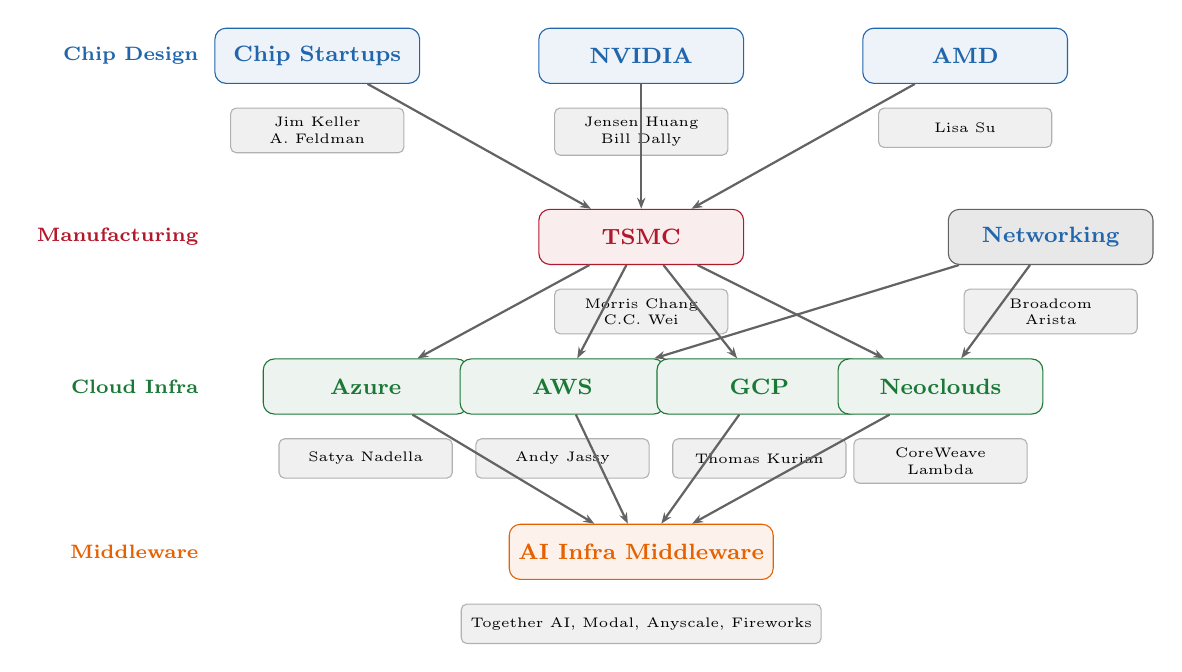
\begin{tikzpicture}[
  node distance=1.2cm,
  company/.style={
    rectangle, rounded corners=4pt,
    draw=figBlue, fill=figBlue!8,
    minimum width=2.6cm, minimum height=0.7cm,
    font=\footnotesize\bfseries, align=center,
    text=figBlue
  },
  person/.style={
    rectangle, rounded corners=2pt,
    draw=figGray!50, fill=figLightGray,
    minimum width=2.2cm, minimum height=0.5cm,
    font=\tiny, align=center
  },
  layer/.style={
    draw=figGray, dashed, rounded corners=6pt,
    inner sep=8pt
  },
  arr/.style={-{Stealth[length=4pt]}, figGray, thick}
]

% Chip Design Layer
\node[company] (nvidia) at (0,0) {NVIDIA};
\node[person, below=0.3cm of nvidia] (jensen) {Jensen Huang\\Bill Dally};

\node[company, right=1.5cm of nvidia] (amd) {AMD};
\node[person, below=0.3cm of amd] (lisa) {Lisa Su};

\node[company, left=1.5cm of nvidia] (startups) {Chip Startups};
\node[person, below=0.3cm of startups] (keller) {Jim Keller\\A. Feldman};

% Manufacturing Layer
\node[company, fill=figRed!8, draw=figRed, text=figRed]
  (tsmc) at (0,-2.3) {TSMC};
\node[person, below=0.3cm of tsmc] (chang) {Morris Chang\\C.C. Wei};

% Cloud Layer
\node[company, fill=figGreen!8, draw=figGreen, text=figGreen]
  (azure) at (-3.5,-4.2) {Azure};
\node[person, below=0.3cm of azure] (nadella) {Satya Nadella};

\node[company, fill=figGreen!8, draw=figGreen, text=figGreen]
  (aws) at (-1,-4.2) {AWS};
\node[person, below=0.3cm of aws] (jassy) {Andy Jassy};

\node[company, fill=figGreen!8, draw=figGreen, text=figGreen]
  (gcp) at (1.5,-4.2) {GCP};
\node[person, below=0.3cm of gcp] (kurian) {Thomas Kurian};

\node[company, fill=figGreen!8, draw=figGreen, text=figGreen]
  (neo) at (3.8,-4.2) {Neoclouds};
\node[person, below=0.3cm of neo] (core) {CoreWeave\\Lambda};

% Middleware Layer
\node[company, fill=figOrange!8, draw=figOrange, text=figOrange]
  (mid) at (0,-6.3) {AI Infra Middleware};
\node[person, below=0.3cm of mid] (togeth) {Together AI, Modal, Anyscale, Fireworks};

% Networking
\node[company, fill=figGray!15, draw=figGray]
  (net) at (5.2,-2.3) {Networking};
\node[person, below=0.3cm of net] (ullal) {Broadcom\\Arista};

% Arrows
\draw[arr] (nvidia) -- (tsmc);
\draw[arr] (amd) -- (tsmc);
\draw[arr] (startups) -- (tsmc);
\draw[arr] (tsmc) -- (azure);
\draw[arr] (tsmc) -- (aws);
\draw[arr] (tsmc) -- (gcp);
\draw[arr] (tsmc) -- (neo);
\draw[arr] (azure) -- (mid);
\draw[arr] (aws) -- (mid);
\draw[arr] (gcp) -- (mid);
\draw[arr] (neo) -- (mid);
\draw[arr] (net) -- (aws);
\draw[arr] (net) -- (neo);

% Layer labels
\node[font=\scriptsize\bfseries\color{figBlue}, anchor=east]
  at (-5.5,0) {Chip Design};
\node[font=\scriptsize\bfseries\color{figRed}, anchor=east]
  at (-5.5,-2.3) {Manufacturing};
\node[font=\scriptsize\bfseries\color{figGreen}, anchor=east]
  at (-5.5,-4.2) {Cloud Infra};
\node[font=\scriptsize\bfseries\color{figOrange}, anchor=east]
  at (-5.5,-6.3) {Middleware};

\end{tikzpicture}
\caption{AI 基础设施权力结构图：从芯片设计到中间件的四层架构，
以及关键人物在各层的分布。箭头表示供应链依赖关系。}
\label{fig:infra-power-structure}
\end{figure}

\begin{keybox}[本章关键人物索引]
\small
\begin{tabularx}{\textwidth}{l l X}
\toprule
\rowcolor{figLightGray}
\textbf{姓名} & \textbf{组织} & \textbf{核心贡献} \\
\midrule
Jensen Huang & NVIDIA CEO & GPU 发明者，NVIDIA 创始人，AI 算力垄断缔造者 \\
Bill Dally & NVIDIA 首席科学家 & 并行计算理论，NVLink 架构 \\
Ian Buck & NVIDIA VP & CUDA 创建者，GPU 通用计算先驱 \\
Bryan Catanzaro & NVIDIA VP & 推动 NVIDIA 拥抱深度学习 \\
Lisa Su & AMD CEO & AMD 史诗级逆袭，Zen 架构，Instinct AI \\
Morris Chang & TSMC 创始人 & 专业代工模式发明者，半导体教父 \\
C.C. Wei & TSMC CEO & TSMC 执行领导，先进工艺量产 \\
Pat Gelsinger & 前 Intel CEO & Intel AI 战略失败的教训 \\
Lip-Bu Tan & Intel 新 CEO & Intel 残酷重启 \\
Jim Keller & Tenstorrent CEO & 传奇芯片架构师，RISC-V 开源革命 \\
Andrew Feldman & Cerebras CEO & 晶圆级芯片创新 \\
Jonathan Ross & Groq 创始人 & TPU 发明者，LPU 确定性推理 \\
Rodrigo Liang & SambaNova CEO & 数据流架构 AI 芯片 \\
Sid Sheth & d-Matrix CEO & 存内计算突破 \\
Nigel Toon & Graphcore CEO & IPU 芯片，SoftBank 收购 \\
Gavin Uberti & Etched CEO & Transformer 专用 ASIC 极端赌注 \\
Satya Nadella & Microsoft CEO & OpenAI 合作，Azure AI 生态 \\
Andy Jassy & Amazon CEO & AWS + Trainium + Anthropic \\
Thomas Kurian & Google Cloud CEO & TPU 商业化，Google Cloud 盈利 \\
Larry Ellison & Oracle 创始人 & AI 数据中心 \$1750 亿赌注 \\
M. Intrator 等 & CoreWeave 创始人 & 从加密矿场到 AI 云 IPO \\
Hock Tan & Broadcom CEO & 定制 AI 芯片，\$1000 亿营收目标 \\
Jayshree Ullal & Arista CEO & AI 数据中心网络女王 \\
Vipul Ved Prakash & Together AI CEO & 推理优化，全明星学术团队 \\
Lin Qiao & Fireworks AI CEO & PyTorch 工程化，开源推理 \\
R. Nishihara & Anyscale CEO & Ray 分布式框架 \\
Erik Bernhardsson & Modal CEO & Serverless GPU 云 \\
Ben Firshman & Replicate 创始人 & Docker Compose + 模型民主化 \\
Stephen Balaban & Lambda Labs CEO & 学术 GPU 云 \\
\bottomrule
\end{tabularx}
\end{keybox}

% =============================================================
% Chapter 10: The Money Behind the Machines — AI Investors and Dealmakers
% Book: AI Figures — Who's Who in the Age of AI
% =============================================================

\chapter{资本推手：AI 投资人与交易操盘者}
\label{ch:investors}

% Chapter overview: The venture capitalists, angel investors, sovereign wealth
% fund managers, and dealmakers whose capital allocation decisions are shaping
% which AI futures get built — and which do not.

如果说前面九章描绘了AI时代的技术创造者和基础设施构建者，本章要回答
一个更本质的问题：\textbf{谁在为这一切提供燃料？}

2025年，全球AI风险投资总额达到2587亿美元，占所有VC投资的61\%。
OpenAI单轮融资1100亿美元、Anthropic累计超过300亿美元、xAI一轮200亿
——这些交易的规模已超越传统风投概念，更像国家级基础设施的资本动员。
在这些天文数字背后，是一小群投资人的判断力、关系网和胆识在决定AI的
方向。他们中有些人在2019年AI尚被嘲笑为"玩具"时就下了重注，有些人则
在2024--2025年的FOMO浪潮中涌入。他们的投资逻辑、认知框架和利益纠葛，
直接塑造了我们看到的AI产业格局。

本章将全面梳理AI投资版图中最重要的人物。从硅谷的传奇风投到中国的创投
教父，从中东主权财富基金的幕后操盘手到独来独往的超级天使，从Y Combinator
的批量孵化到Stargate项目的五千亿美元豪赌——每一笔重大交易背后都有一个
具体的人做出了具体的决定。理解这些人，就是理解AI资本的运行逻辑。

\begin{whybox}[为什么AI投资人值得单独一章？]
在大多数技术叙事中，资本被简化为"背景板"——某公司融了多少钱，估值
多少。但在AI时代，投资人的角色远不止于提供资金：
\begin{enumerate}
  \item \textbf{路径选择者}：Vinod Khosla在2019年给OpenAI写下5000万美元
    支票时，OpenAI还是一个没有商业模式的非营利研究实验室。如果没有这笔
    资金，Sam Altman可能无法推动OpenAI向营利结构转型，整个GPT系列的
    发展轨迹可能完全不同。
  \item \textbf{治理参与者}：Reid Hoffman曾担任OpenAI董事，参与了多次关键
    治理决策。Josh Kushner的Thrive Capital在OpenAI的董事会安排中拥有
    重要话语权。投资人不只是签支票，他们还参与——有时甚至主导——AI公司
    的战略方向。
  \item \textbf{叙事塑造者}：Marc Andreessen的"Why AI Will Save The World"
    一文塑造了整个行业对AI风险与收益的讨论框架。a16z的Martin Casado关于
    "Bitter Economics"的分析改变了投资者对AI公司资本结构的理解。
  \item \textbf{地缘政治棋手}：MGX、GIC、QIA等主权基金的入局，让AI投资
    成为地缘政治博弈的一部分。Abu Dhabi和沙特正通过AI投资将石油财富转化
    为技术影响力。
\end{enumerate}
因此，理解这些人不仅是"八卦"，更是理解AI产业结构的必要条件。
\end{whybox}


% =============================================================
\section{十亿美元支票：谁在写AI史上最大的交易？}
\label{sec:inv-megarounds}
% =============================================================

在传统风险投资中，一笔1亿美元的交易就算"超级轮次"。但在2024--2026年的
AI融资市场中，十亿美元只是入场券。让我们从最大的交易开始，认识操盘这些
交易的关键人物。

\subsection{孙正义与SoftBank：从Vision Fund的废墟到AI的最大赌徒}
\label{subsec:inv-masa}

\begin{corebox}[人物档案：孙正义（Masayoshi Son）]
\textbf{身份}：SoftBank Group创始人兼CEO \\
\textbf{生于}：1957年，日本佐贺县鸟栖市的韩裔日本人家庭 \\
\textbf{教育}：加州大学伯克利分校经济学学士 \\
\textbf{AI关键角色}：Stargate Project联席主席；OpenAI最大外部投资者之一 \\
\textbf{投资风格}：极端集中、超高杠杆、"300年愿景"
\end{corebox}

孙正义（Masayoshi Son）是全球科技投资史上最具争议的人物之一。他的投资
生涯由两个极端定义：1990年代的雅虎和阿里巴巴投资让他一度成为世界首富，
2019--2021年Vision Fund的WeWork、Wirecard等灾难性投资则让他蒙受了
数百亿美元的亏损。但在AI时代，孙正义再次All-in。

\textbf{OpenAI豪赌。}2025年3月，SoftBank承诺向OpenAI投资高达400亿美元
——这是科技史上最大的单一投资者承诺。第一批75亿美元在2025年4月到位，
剩余225亿美元在2025年12月完成，使SoftBank在OpenAI的持股比例达到约11\%。
通过Vision Fund 2执行，SoftBank还引入了110亿美元的联合投资者。到2026年2月
OpenAI宣布1100亿美元新一轮融资时，SoftBank再次投入300亿美元——累计对
OpenAI的直接投资超过700亿美元。

\textbf{Stargate项目。}2025年1月，在白宫的一场活动中，孙正义与Sam Altman
共同宣布了"Stargate项目"——一个5000亿美元的AI基础设施联合投资计划。
参与方包括OpenAI（40\%股权）、SoftBank（40\%股权）、Oracle和MGX。
孙正义担任Stargate LLC的联席主席。SB Energy（SoftBank全资子公司）将在
德克萨斯州建设1.2吉瓦的数据中心和电力基础设施。这个项目的规模等同于
一个中等国家的能源基础设施投入。

\textbf{投资逻辑。}孙正义的AI投资逻辑可以用他自己2024年在SoftBank World
上的讲话概括："ASI（Artificial Super Intelligence）将在10年内到来，
而OpenAI是最有可能率先到达那里的公司。我要用尽一切资源，确保SoftBank
站在ASI到来时的正确位置。"这种"赌国运"式的投资风格让他在Vision Fund 1.0
时代栽了大跟头（WeWork、Oyo等），但如果OpenAI和Stargate的故事最终
成立，孙正义的AI赌注可能成为投资史上回报最高的一笔。

\begin{warnbox}[SoftBank的OpenAI投资已经赚钱了吗？]
表面上看是的。2026年2月，SoftBank在Vision Fund的季度报告中公布了42亿美元的
OpenAI投资增值。但这是纸面收益——直到OpenAI完成IPO（预计2026年底至
2027年初），SoftBank无法变现。更大的风险在于：SoftBank为了集中资源投资
AI，大幅减持了其他资产（包括部分ARM股权），杠杆率居高不下。如果AI估值
出现修正，SoftBank的整体财务状况可能迅速恶化。孙正义本人的净资产与
SoftBank股价高度绑定——这是真正的All-in。
\end{warnbox}


\subsection{Josh Kushner与Thrive Capital：OpenAI最亲密的金融伙伴}
\label{subsec:inv-thrive}

\begin{corebox}[人物档案：Josh Kushner]
\textbf{身份}：Thrive Capital创始人兼管理合伙人 \\
\textbf{生于}：1985年，美国新泽西州 \\
\textbf{教育}：哈佛大学 \\
\textbf{AI关键角色}：OpenAI最早期的机构投资者之一；多轮领投或重要参投 \\
\textbf{投资风格}：成长期、收入驱动、长期伙伴关系 \\
\textbf{净资产}：估计超过40亿美元
\end{corebox}

Josh Kushner在2011年创立Thrive Capital时只有26岁。过去十五年中，Thrive
投资了Instagram、Spotify、Stripe等定义时代的科技公司。但真正让Kushner
跻身AI投资最核心圈层的是他与Sam Altman的关系，以及对OpenAI的持续加注。

\textbf{OpenAI投资时间线：}
\begin{itemize}
  \item \textbf{2023年}：Thrive领导了一轮OpenAI二级市场交易，估值860亿美元
    ——这是Kushner首次大规模介入OpenAI；
  \item \textbf{2024年10月}：Thrive参与了OpenAI 66亿美元融资轮，
    投资约13亿美元，Kushner公开表示"因为两个关键原因下注"；
  \item \textbf{2025年3月}：参与OpenAI 400亿美元轮次；
  \item \textbf{2025年12月}：以2850亿美元估值单独投资约10亿美元
    ——当时OpenAI已在讨论以8300亿美元估值的更大轮次，这意味着
    Thrive的这笔投资一入账就"已经在赚钱"（in the money）；
  \item \textbf{2026年2月}：预计参与1100亿美元轮次。
\end{itemize}

Kushner的成功不仅在于投资眼光，更在于关系经营。Sam Altman对Kushner的
评价是："Extremely grateful to work with Josh. No one could ask for a more
committed, more thoughtful, or harder-working investor."这种密切关系让
Thrive获得了其他基金难以比拟的优先配额权——在AI融资市场中，
\textbf{拿到配额往往比选对公司更难}。

2026年2月，Thrive宣布关闭了其最新基金，规模超过100亿美元——这使
Thrive成为仅有的几家单只基金突破百亿的成长期基金之一。OpenAI也
反向入股了Thrive，双方的利益深度绑定。

\begin{whybox}[为什么Thrive能获得OpenAI的"特殊交易"？]
2025年12月，Thrive以2850亿美元估值投资OpenAI——几个月后OpenAI就以
8400亿美元估值融资。这种"优惠价"引发了市场争议。《华尔街日报》报道，
这种不同投资者获得不同条件的做法在AI融资中越来越常见——核心原因是
AI公司需要的资金规模如此之大，以至于它们需要"锚定投资者"来建立市场
信心。Thrive作为OpenAI最长期的财务投资者，扮演了这个角色。代价是
什么？后进投资者可能需要接受更高的估值和更弱的保护条款——这实际上是
用"不平等"的交易条件来奖励忠诚度和长期承诺。
\end{whybox}


% =============================================================
\section{硅谷AI权力掮客}
\label{sec:inv-sv-power}
% =============================================================

如果说孙正义和Kushner代表了"大支票"投资者，本节介绍的人物则代表了
硅谷AI投资的思想领导力——他们不仅投资金，更投信念和愿景。

\subsection{Marc Andreessen：AI乐观主义的旗手}
\label{subsec:inv-marc}

\begin{corebox}[人物档案：Marc Andreessen]
\textbf{身份}：Andreessen Horowitz（a16z）联合创始人兼普通合伙人 \\
\textbf{生于}：1971年，美国爱荷华州 \\
\textbf{教育}：伊利诺伊大学厄巴纳-香槟分校计算机科学学士 \\
\textbf{早期成就}：Mosaic浏览器创建者；Netscape联合创始人 \\
\textbf{AI关键角色}：a16z AI投资战略总设计师；AI政策倡导者 \\
\textbf{代表性文章}："Why AI Will Save The World"（2023年6月）
\end{corebox}

Marc Andreessen可能是当代科技投资界最具思想影响力的人物。他在1993年
共同创建了Mosaic浏览器（后来的Netscape），直接催生了互联网时代。
2009年与Ben Horowitz共同创立a16z后，他提出的"Software Is Eating The
World"（2011年《华尔街日报》专栏）成为过去十年科技投资的核心论述。
进入AI时代，Andreessen再次扮演了叙事塑造者的角色。

\textbf{``Why AI Will Save The World''——AI时代的宣言书。}2023年6月，
Andreessen在a16z网站上发表了长文"Why AI Will Save The World"，系统性地
反驳了AI威胁论，主张AI将"增强而非取代人类智能"，并将AI监管描述为
"既有利益集团保护护城河的工具"。这篇文章迅速成为AI投资圈的"必读文本"
——无论你是否同意其观点，它为AI乐观主义提供了一个完整的论证框架。

\textbf{a16z的AI投资版图。}在Andreessen的战略指导下，a16z在AI领域的
部署堪称全方位：
\begin{itemize}
  \item OpenAI——据报道投资超过100亿美元；
  \item Anthropic——据报道投资约40亿美元；
  \item Databricks, Scale AI——数据基础设施层；
  \item Cursor（代码AI，估值500亿美元的开发者工具）；
  \item ElevenLabs——语音合成AI领头羊；
  \item Character.AI——消费者AI应用；
  \item Mistral AI——欧洲最重要的基础模型公司。
\end{itemize}

a16z的管理资产（AUM）已超过900亿美元，使其成为全球最大的科技风投基金。
2025年，a16z在AI领域参与了超过25笔交易，单笔投资规模从500万到5亿美元
不等。

2026年1月，Andreessen在播客中进一步阐述了他对AI时代的看法："2025年
可能是科技史上最重要的一年……这不是渐进式改进，而是从零到一的转变。
AI正在重新定义产品经理、设计师和工程师的角色。"

\textbf{政治参与。}Andreessen在2024年美国大选中公开支持特朗普，
这一举动在硅谷引发了强烈争议。他的政治立场与AI政策主张紧密关联：
反对过度监管、支持"Little Tech"、反对FARA等对创业公司构成合规负担
的法规。他与Ben Horowitz共同推出的"The Little Tech Agenda"将AI监管
批评扩展为更广泛的科技政策框架。

\begin{keybox}[a16z AI团队核心人物]
\small
\begin{tabularx}{\textwidth}{l l X}
\toprule
\rowcolor{figLightGray}
\textbf{姓名} & \textbf{角色} & \textbf{关键贡献} \\
\midrule
Marc Andreessen & 联合创始人 & AI战略总设计师，"Why AI Will Save The World" \\
Ben Horowitz    & 联合创始人 & a16z文化构建者，2024年政治参与 \\
Martin Casado   & 普通合伙人 & AI基础设施投资论文，"Bitter Economics"分析 \\
Anjney Midha    & 风险合伙人 & GPU分配决策者，Mistral/BFL董事，AMP创始人 \\
Matt Bornstein  & 合伙人 & AI应用层投资，AI基础设施堆栈分析 \\
\bottomrule
\end{tabularx}
\end{keybox}

\paragraph{Martin Casado——AI基础设施的思想家}

Martin Casado在2015年以普通合伙人身份加入a16z之前，是SDN（软件定义
网络）领域的先驱——他创立的Nicira在2012年被VMware以12.6亿美元收购。
在a16z，Casado成为AI基础设施投资的核心驱动力。

2025年11月，Casado发表了极具影响力的文章"Bitter Economics"，将Richard
Sutton的"The Bitter Lesson"（计算胜过巧妙算法）扩展到商业层面：
AI系统本质上是"将大量资本转化为可工作的解决方案"，这从根本上改变了
软件公司的资本结构。传统软件公司的边际成本趋近于零，但AI公司的边际
成本（推理算力）始终存在——这意味着AI公司更像资本密集型企业而非
软件公司。这一洞见深刻影响了投资者对AI公司估值的理解。

2026年1月，Casado在播客中进一步解释了AI需求侧的驱动力：当前的约束
更多来自监管（电力、数据中心、算力扩张方面的限制），而非技术本身。
AI Agent工具可能将基础设施决策从人类转移到智能体——这将是基础设施
投资的下一个重大转折点。

\paragraph{Anjney Midha——算力的守门人}

Anjney Midha的职业轨迹揭示了AI时代一个鲜为人知但极其重要的权力节点：
\textbf{算力分配权}。

Midha在2023年加入a16z后，负责管理公司的"Oxygen"项目——一个超过
20000块GPU的私有算力集群。在GPU严重短缺的2023--2024年，Midha决定哪些
AI创业公司能获得a16z的算力支持——这实质上是在决定哪些公司能生存。
他同时担任Mistral AI（欧洲最大的开源LLM公司，估值140亿美元）和Black
Forest Labs（德国图像生成AI公司，估值32.5亿美元）的董事。

2024年10月，Midha宣布创立AMP——一家独立的"算力+资本"公司，为前沿AI
团队同时提供GPU资源和投资。他继续以风险合伙人身份留在a16z。这一举动
暴露了AI时代的一个根本真相：\textbf{在算力成为稀缺资源的时代，算力
分配者拥有的权力可能不亚于资本分配者}。Midha年仅33岁，已经坐在了
AI世界的一个关键交叉点上。


\subsection{Vinod Khosla：AI史上最成功的单笔投资}
\label{subsec:inv-khosla}

\begin{corebox}[人物档案：Vinod Khosla]
\textbf{身份}：Khosla Ventures创始人 \\
\textbf{生于}：1955年，印度新德里 \\
\textbf{教育}：IIT Delhi电气工程学士；卡内基梅隆大学生物医学工程硕士；
  斯坦福大学商学院MBA \\
\textbf{早期成就}：Sun Microsystems联合创始人 \\
\textbf{AI关键投资}：OpenAI（2019年5000万美元→2026年价值约80亿美元，160倍回报） \\
\textbf{投资风格}："黑天鹅猎人"——押注科学实验级别的颠覆性技术
\end{corebox}

Vinod Khosla对OpenAI的投资可能是风险投资史上最成功的单笔交易之一。

\textbf{故事从Elon Musk的退出开始。}2019年，OpenAI正处于生死关头。
作为非营利组织成立四年后，OpenAI面临一个根本性矛盾：深度学习研究需要
海量算力，但非营利架构限制了其筹资能力。联合创始人Elon Musk在2018年
退出董事会后，还留下了对10亿美元资金承诺的不确定性。Sam Altman需要
找到新的资金来源来支撑OpenAI的野心。

Khosla此时入场。据Fortune报道，在Musk犹豫之际，Khosla果断写下了5000万
美元的支票——这是他40年投资生涯中最大的单笔初始投资。The Information
报道，这笔投资换取了OpenAI约5\%的股权。到2026年初，以OpenAI 8400亿美元
的估值计算，这笔投资价值约80亿美元——回报率约160倍。

\textbf{这不是运气，是认知框架。}Khosla的投资哲学可以用"指数套利"
（Exponential Arbitrage）来概括：当技术进步的速度是指数级的，而大多数人
的认知仍然是线性的，指数与线性之间的差距就是巨大的投资机会。2019年的
OpenAI正处于这样一个认知差距中——GPT-2已经展示了语言模型的惊人潜力，
但绝大多数投资者仍然认为AI是"学术玩具"。

Khosla在2019年看到的，是GPT-2到GPT-3的"跃迁"——同样的架构，更多的
算力和数据，能力呈指数级增长。他赌的不是某个具体产品，而是scaling laws
——算力投入和模型能力之间的幂律关系会持续成立。事实证明，他对了。

\textbf{持续加注。}Khosla不仅在2019年下了初始注，还在后续轮次中持续
加注。2024年10月，Khosla Ventures通过SPV（特殊目的载体）为OpenAI的66亿
美元轮次额外筹集了4.05亿美元。值得注意的是，这4.05亿中的大部分来自
外部投资者——Khosla利用自己的配额权帮助其他渴望参与OpenAI的投资者
获得入场券。这种模式在AI融资中越来越常见：顶级VC的核心价值不仅在于
自己的资金，更在于\textbf{分配稀缺配额的权力}。

\textbf{AI预言。}Khosla是AI领域最大胆的预言者之一。他公开预测到2030年
80\%的现有工作岗位将被AI取代——同时强调这将创造"前所未有的繁荣"。
2026年3月，他在Fortune的采访中讨论了谁在AI竞赛中领先，表达了对OpenAI
保持领先地位的信心，同时也强调了美国需要加速AI发展以在全球竞争中
保持优势。


\subsection{Reid Hoffman：AI生态系统的连接者}
\label{subsec:inv-hoffman}

\begin{corebox}[人物档案：Reid Hoffman]
\textbf{身份}：Greylock Partners合伙人；LinkedIn联合创始人 \\
\textbf{生于}：1967年，美国加利福尼亚州 \\
\textbf{教育}：斯坦福大学符号系统学士；牛津大学硕士 \\
\textbf{AI关键角色}：OpenAI早期董事会成员和投资者；Anthropic投资者；
  AI政策倡导者 \\
\textbf{标签}：``PayPal Mafia''成员；``硅谷的外交官''
\end{corebox}

Reid Hoffman的独特之处在于，他可能是AI领域中同时押注了最多"竞争对手"
的投资者。作为个人投资者和Greylock合伙人，Hoffman同时投资了OpenAI和
Anthropic——两家正面竞争的AI公司。

\textbf{OpenAI的早期支持者。}Hoffman是OpenAI最初的捐赠者和董事会成员之一，
参与了OpenAI从非营利到营利结构转型的关键决策。他在OpenAI董事会一直任职
到2023年，期间经历了包括Sam Altman短暂被解雇又复职的戏剧性事件。

\textbf{同时投资Anthropic。}2025年10月，当AI和加密沙皇David Sacks公开
批评Anthropic时，Hoffman公开为Anthropic辩护，称其为"好人之一"（one of
the good guys），并表示："Anthropic与Microsoft、Google和OpenAI一样，正在
以正确的方式部署AI——深思熟虑、安全且对社会有巨大益处。"他同时确认
Greylock已投资Anthropic。

这种"两边下注"的策略在传统VC中会引发利益冲突质疑，但在AI领域却越来越
普遍——因为投资者的共识是：AI市场足够大，容得下多个赢家。Hoffman的
核心信念是AI本身的转型力量，而非某家特定公司的胜出。

\textbf{思想影响力。}Hoffman是AI领域最多产的公共知识分子之一。他共同
撰写了多本书，包括与GPT-4合作撰写的《Impromptu: Amplifying Our Humanity
Through AI》。他的播客和专栏持续探讨AI对社会、就业和民主的影响。
与Andreessen的纯乐观主义不同，Hoffman更倾向于"cautious optimism"
——承认AI的风险，但相信通过负责任的开发可以最大化收益。


\subsection{Sequoia Capital：AI投资的系统化玩家}
\label{subsec:inv-sequoia}

\begin{corebox}[Sequoia Capital AI投资概览]
\textbf{管理资产}：超过900亿美元 \\
\textbf{2025年AI交易数}：20+ \\
\textbf{代表性AI投资}：Anthropic, xAI, Scale AI, Glean, ElevenLabs,
  Hugging Face, Mistral AI \\
\textbf{2026年AI VC排名}：顶级（Earthian AI、PitchBook等多个排名）
\end{corebox}

\paragraph{Roelof Botha——稳健的舵手}

Roelof Botha自2003年加入Sequoia以来，逐步成为硅谷最受尊敬的投资人之一。
出生于南非，Botha早年在PayPal担任CFO（与Elon Musk、Peter Thiel共事），
之后加入Sequoia。他领导了对YouTube、Instagram、MongoDB等公司的早期投资。

在AI时代，Botha带领Sequoia迅速布局——Anthropic的多轮融资、xAI、Scale AI
等关键交易都有Sequoia的身影。2025年11月，Botha在任职近十年后将Sequoia
的"管家"（steward）角色移交给Pat Grady和Alfred Lin。Bloomberg报道，
这一决定是合伙人一致做出的，Grady和Lin计划在Botha的基础上"深化对AI的
聚焦"，同时降低公司的政治化形象。

\paragraph{Pat Grady——Sequoia的AI操盘手}

Pat Grady是Sequoia AI战略的实际操盘者。2007年，24岁的Grady加入Sequoia
后，靠的不是天才的投资直觉，而是"笨功夫"——每天打50个陌生电话
（cold calls），系统性地扫描潜在投资标的。他在2024年公开分享了Sequoia
早年投资ServiceNow的CRM记录："left message with assistant"、
"sent email"、"left voice mail"——一周又一周的坚持，直到Fred Luddy
终于回电。

Grady与另一位合伙人Sonya Huang共同在Sequoia官网上发表公开信，邀请
AI创始人直接向他们发送想法和pitch——这种"开放式招商"的方式在顶级VC中
极为罕见。Business Insider将Grady列入2024年AI Power List，评价他
"比任何人都更深入地领导了Sequoia的AI战略"。

2025年11月，43岁的Grady成为Sequoia的联席管家（co-steward）。他的升任
标志着Sequoia明确将AI作为未来十年的核心投资方向。

\begin{whybox}[Sequoia对AI交易的态度：不追求好价格]
Grady曾对Business Insider说："We don't make money by getting a good deal."
——Sequoia的成功不是靠在估值上占便宜，而是靠投对人。这种哲学在AI时代
尤为重要：当OpenAI估值8400亿、Anthropic估值3800亿时，纠结于某轮融资的
估值差异几乎没有意义——真正的问题是这些公司能否在未来十年创造数千亿
美元的收入。如果答案是肯定的，那么在1000亿还是1200亿估值时入场的差异
微不足道。
\end{whybox}


\subsection{超级天使与双重身份投资者}
\label{subsec:inv-angels}

AI时代产生了一类独特的投资者：他们既是技术从业者（创始人、工程师、
高管），又是活跃的天使投资人。他们的投资判断往往源于对技术的第一手理解，
而非传统的财务分析。

\paragraph{Daniel Gross与Nat Friedman：从投资人到被收购者}

Daniel Gross和Nat Friedman的故事是AI时代最戏剧性的投资人叙事之一。

Gross早年在Apple担任AI和机器学习主管，之后创立了Pioneer（一个在线
创业加速器）。Friedman则是GitHub的前CEO，在Microsoft收购GitHub的过程中
发挥了关键作用。两人于2021年联合创立了NFDG（Nat Friedman \& Daniel Gross），
一个专注AI的风投基金，投资了Perplexity、The Bot Company等热门公司。

2024年6月，Gross成为Safe Superintelligence（SSI）的联合创始人兼CEO——
SSI由OpenAI联合创始人Ilya Sutskever发起，专注于开发"安全的超级智能"，
估值迅速攀升至320亿美元。这使Gross从投资者变成了创始人。

然后事情发生了戏剧性转折。2025年6月，Meta试图以320亿美元收购SSI
——被Sutskever拒绝。收购失败后，Zuckerberg改为直接挖人：Meta聘请了
Gross和Friedman，同时部分收购了NFDG基金的份额，获得了该基金所投AI
创业公司的少数股权。这一系列操作展示了AI时代的一个新现象：
\textbf{投资人本身成为了被收购的目标}——因为他们的关系网、技术洞察力
和所持有的投资组合，比任何单笔投资都更有价值。

\paragraph{Elad Gil：一个人的多十亿帝国}

Elad Gil可能是AI时代最成功的solo investor（单人投资者）。他的职业轨迹
从Google早期员工（负责Google Maps和Gmail等移动产品）到Twitter高管
（通过收购其创立的Mixer Labs加入），再到全职天使投资人。

2024年，Gil筹集了10亿美元的新基金，使其个人可投资资金超过20亿美元。
他的AI投资组合涵盖了几乎所有热门赛道：
\begin{itemize}
  \item \textbf{基础模型}：OpenAI, Mistral；
  \item \textbf{AI应用}：Harvey（法律AI）, Pika（视频生成）,
    Perplexity（AI搜索）；
  \item \textbf{AI基础设施}：Magic（代码生成）；
  \item \textbf{防务AI}：Helsing（欧洲AI防务独角兽）。
\end{itemize}

2025年11月在TechCrunch Disrupt大会上，Gil分享了他的AI投资哲学：
"AI是我见过的最不可预测的技术浪潮之一……我在2021年开始投资生成式AI，
当时几乎没人关注。GPT-2到GPT-3的跃迁如此巨大，如果你只是沿着
scaling laws外推，就能看到这将变得极其重要。"

Gil的投资风格有一个显著特征：\textbf{当他出现在cap table上时，估值
立刻上升}。更大的投资者知道，如果Elad已经投了，那这家公司值得认真
看——这是一种强大的信号效应。

\paragraph{Naval Ravikant：哲学投资家}

Naval Ravikant作为AngelList的创始人，不仅是AI投资者，更是整个天使投资
基础设施的构建者。AngelList使得小额天使投资人能够高效地参与创业公司
融资——在AI时代，数百个AI创业公司通过AngelList的Rolling Funds和
Syndicates获得了种子资金。

Ravikant的投资哲学更接近于一种技术哲学：他在Twitter上广泛讨论AI对
人类认知、工作和意义的影响。他的核心观点是AI将使"杠杆"（leverage）
民主化——以前只有资本和劳动力能产生杠杆，现在代码和AI为每个人提供了
无限杠杆。这种思想框架影响了一整代AI创业者的自我认知和创业方向。

\paragraph{Eric Schmidt：从Google CEO到AI战略家}

Eric Schmidt的身份转变可能是科技史上最引人注目的之一——从全球最大
AI公司之一（Google）的掌门人，到独立的AI投资者、政策倡导者和创业者。

\textbf{投资与创业。}Schmidt离开Google后，通过个人投资和Schmidt Futures
（其慈善科技基金）广泛投资AI领域。他还共同创立了Relativity Space，
并担任CEO。但他最大的影响力来自\textbf{政策层面}：他曾领导美国国家
人工智能安全委员会（NSCAI），该委员会在2021年发布的报告深刻影响了
美国的AI战略方向。

\textbf{AI地缘政治论述。}2025年12月，Schmidt在Time杂志发表文章
"How the U.S. Can Win the AI Race"，提出AI竞赛实际上是多个重叠的竞赛
——美中AGI竞争、AI应用普及竞争、AI治理竞争。他指出中国的AI+计划
目标到2030年实现90\%的关键行业AI整合，而美国在AI采用率上反而落后于
中国（中国60\%的员工每周使用AI，美国仅37\%）。

2026年3月，Schmidt在Fortune发表专栏，主张科技巨头应该建设与电力源共址
的数据中心（co-located data centers），而非依赖公共电网——直接回应了
公众对AI数据中心推高电费的担忧。这种从投资者到政策倡导者的角色转换，
使Schmidt成为AI时代最独特的"混合身份"人物之一。

\paragraph{Jeff Bezos：低调的AI多头}

Jeff Bezos可能是AI领域投资规模最大但最低调的个人投资者。通过Bezos
Expeditions（其个人投资工具），Bezos在OpenAI成立初期就参与了资助
——他是2015年最早向OpenAI捐款的科技领袖之一。

但Bezos更大的AI投资是通过Amazon完成的——Amazon对Anthropic的累计投资
承诺达到80亿美元。到2025年2月，Amazon在Anthropic的持股价值已升至约
140亿美元，账面增值约60亿美元（75\%回报率）。此外，Amazon在2026年2月
以500亿美元参与了OpenAI的1100亿美元融资——标志着Amazon从"Anthropic独家
盟友"转变为"AI双头下注"的策略。

\paragraph{Peter Thiel与Founders Fund：从谨慎到All-in}

Peter Thiel的AI投资之路经历了一个有趣的转变。Founders Fund最初对
生成式AI持"谨慎观望"态度——这对一家以"Contrarian"著称的基金来说
并不意外。但到2025年下半年，Founders Fund转向了"集中押注"模式。

Founders Fund的AI投资组合反映了Thiel一贯的"与国家竞争"
（competing with nation-states）论述：
\begin{itemize}
  \item \textbf{Anthropic}：参与了\$30B Series G融资的联合领投方之一；
  \item \textbf{Anduril}：AI防务系统公司，\$25亿Series G；
  \item \textbf{Scale AI}：AI数据基础设施，\$10亿Series F；
  \item \textbf{Crusoe Energy}：AI数据中心能源公司，\$5亿融资；
  \item \textbf{Hadrian}：AI驱动的精密制造。
\end{itemize}

2026年3月，Founders Fund正在筹集60亿美元的新基金（Growth IV），预计
将大幅加重AI在投资组合中的比重。Thiel的AI投资论述可以概括为：
\textbf{AI不是一般意义上的技术投资，而是关乎美国国家安全的战略资产}。
这种框架与他在Palantir的创始经历和长期的国防投资偏好一脉相承。


\subsection{Y Combinator：AI创业的批量生产线}
\label{subsec:inv-yc}

\begin{corebox}[人物档案：Garry Tan]
\textbf{身份}：Y Combinator CEO \\
\textbf{生于}：1981年，加拿大温尼伯，华裔 \\
\textbf{教育}：斯坦福大学计算机系统工程学士 \\
\textbf{早期经历}：Palantir第10号员工；Posterous联合创始人
  （被Twitter收购）；Initialized Capital联合创始人 \\
\textbf{AI关键角色}：重塑YC为AI创业首选加速器
\end{corebox}

Garry Tan于2023年接任Y Combinator CEO后，迅速将这个传统的创业加速器
转变为AI创业的核心枢纽。在他的领导下，YC每个批次中AI公司的比例从2023年
的约32\%飙升至2025年的67\%以上。

\textbf{AI改变了YC的选人标准。}2026年3月在SXSW的演讲中，Tan透露AI正在
根本性地改变YC评估申请者的方式。当编程智慧"随手可得"（on tap），加速器
更看重创始人的\textbf{品味、行动力和产品管理能力}。"下一个伟大的发明者
可能是英语专业的学生"——这句话标志着创业门槛的范式转变。

Tan本人也是AI工具的狂热用户。他在SXSW上对Bill Gurley说自己只睡四个
小时，因为太兴奋于和AI Agent协作。"我可以做我的全职工作——八九个小时
的会议——同时在三个不同项目上完成10000行代码。"他开玩笑说自己得了
"cyber psychosis"（AI引起的兴奋失眠）。

YC的每个批次为每家公司提供50万美元的种子资金和13周的加速指导。更重要的是
YC的网络效应：Airbnb、DoorDash、Coinbase、Instacart等超级独角兽都出自
YC——这种校友网络为AI创业公司提供了客户、合作伙伴和后续融资的巨大优势。


% =============================================================
\section{中国AI投资版图}
\label{sec:inv-china}
% =============================================================

中国的AI投资生态与硅谷有着根本性的差异：更深的政府参与、更紧密的产业-
资本联动、以及地缘政治对跨境投资的严重制约。在这个生态中，一小群投资人
扮演着特殊的"翻译者"角色——在中国和全球科技之间架桥。

\subsection{沈南鹏（Neil Shen）：两个世界之间的桥梁}
\label{subsec:inv-shen}

\begin{corebox}[人物档案：沈南鹏（Neil Shen）]
\textbf{身份}：红杉中国/HongShan（HSG）创始及管理合伙人 \\
\textbf{生于}：1967年，浙江海宁 \\
\textbf{教育}：上海交通大学应用数学学士；耶鲁管理学院硕士 \\
\textbf{早期成就}：携程旅行网（Ctrip）联合创始人；如家酒店连锁联合创始人 \\
\textbf{AI关键角色}：中国AI投资规模最大、影响力最深的单一投资人 \\
\textbf{净资产}：约38亿美元（2025年9月Forbes估算） \\
\textbf{管理资产}：约560亿美元
\end{corebox}

沈南鹏是中国风险投资史上最成功的人物——这一点得到了Forbes和
Financial Times的一致认可。他在2005年创立红杉资本中国后，投资了
包括美团、字节跳动、拼多多等定义中国互联网时代的公司。

\textbf{从红杉中国到HongShan的独立。}2023年，全球红杉拆分为三个独立
实体——美国Sequoia Capital、中国HongShan（原Sequoia China）和
印度/东南亚Peak XV。沈南鹏领导的HongShan成为完全独立的投资机构。这次
拆分反映了中美地缘政治紧张的深远影响：美国LP（有限合伙人）越来越不愿
让自己的资金流入中国科技公司，而中国政府也在审视美资对国内科技企业的
影响力。

\textbf{AI投资布局。}在AI时代，沈南鹏的HongShan依然是中国AI领域最重要
的资本力量。2026年2月，《华尔街日报》以"将美国资本注入中国AI的香港
投资人"（The Hong Kong Investor Putting American Money Into China's AI
Push）为题报道了沈南鹏如何继续利用美国资本支持中国AI公司——尽管
面临越来越大的地缘政治压力。

HongShan在AI领域的投资覆盖了中国AI生态的几乎所有关键层：
\begin{itemize}
  \item \textbf{基础模型}：月之暗面（Moonshot AI）、智谱AI（Zhipu AI）等
    中国头部大模型公司；
  \item \textbf{AI应用}：多个垂直领域的AI应用创业公司；
  \item \textbf{AI基础设施}：芯片、算力、数据相关的创业公司。
\end{itemize}

沈南鹏的核心挑战在于：如何在中美技术脱钩的趋势下，继续维持中国AI
创业公司获取全球资本和技术的通道？HongShan将总部设在香港而非北京或
上海，本身就是一种策略性安排——香港作为中间地带，为跨境资本流动提供
了一个虽然收窄但仍然存在的通道。


\subsection{张磊（Zhang Lei）：从耶鲁到中国AI工厂}
\label{subsec:inv-zhanglei}

\begin{corebox}[人物档案：张磊（Zhang Lei）]
\textbf{身份}：高瓴投资（Hillhouse Investment）创始人兼CEO \\
\textbf{生于}：1972年，中国河南省驻马店市 \\
\textbf{教育}：中国人民大学学士；耶鲁管理学院MBA \\
\textbf{早期成就}：2005年用耶鲁大学捐赠基金提供的2000万美元创立高瓴 \\
\textbf{管理资产}：超过150亿美元（公开市场合并基金） \\
\textbf{AI观点}："中国已成为世界的AI工厂"
\end{corebox}

张磊和高瓴在中国投资界的地位类似于Sequoia在硅谷的角色——以长期主义和
研究驱动著称。高瓴早期以投资腾讯和京东而闻名，管理过超过180亿美元的
旗舰私募基金。

\textbf{AI战略定位。}在AI时代，张磊的策略与多数纯财务投资者不同——
他更强调"AI+产业"的融合。2025年10月，张磊在Global Financial Leaders'
Investment Summit上表示："中国将最先在AI应用层实现大规模变现。"
他的论点是：中国虽然在基础模型的绝对能力上可能暂时落后于美国
（OpenAI、Anthropic、Google的模型在某些benchmark上领先），但在
\textbf{AI应用的速度和广度}上，中国已经领先。

2025年9月，高瓴的风险投资部门GL Ventures与浦东创投共同成立了20亿元人民币
（约2.8亿美元）的AI专项基金，支持上海张江AI创新小镇的建设，目标是
孵化1000家AI公司。这种"产业+资本+地方政府"的三角合作模式是中国AI投资
的典型特征——与硅谷纯市场驱动的模式形成鲜明对比。

2025年11月，张磊将高瓴旗下三只公开市场基金合并为一只超过150亿美元的
综合基金——这是多年来最大规模的内部重组，旨在让投资组合更加灵活。
在AI领域，高瓴的投资覆盖了自动驾驶（地平线机器人）、AI制造、AI医疗等
"重型应用"赛道。


\subsection{李开复（Kai-Fu Lee）：科学家、投资人、创业者的三重身份}
\label{subsec:inv-kaifulee}

\begin{corebox}[人物档案：李开复（Kai-Fu Lee）]
\textbf{身份}：创新工场（Sinovation Ventures）董事长兼CEO；01.AI创始人兼CEO \\
\textbf{生于}：1961年，台湾台北 \\
\textbf{教育}：哥伦比亚大学计算机科学学士；卡内基梅隆大学计算机科学博士 \\
\textbf{职业路径}：Apple VP → SGI VP → Microsoft Corp VP →
  Google中国区总裁 → 创新工场创始人 → 01.AI创始人 \\
\textbf{代表作}：《AI Superpowers》《AI 2041》 \\
\textbf{管理资产}：约30亿美元（双币种基金）
\end{corebox}

李开复是AI领域罕见的"三栖人物"——他同时是顶级的AI研究者（博士论文创建了
世界上第一个不依赖特定说话人的连续语音识别系统SPHINX）、活跃的投资者
（创新工场管理30亿美元基金）和一线创业者（01.AI）。

\textbf{从投资者到创业者。}2023年，李开复做出了令投资圈惊讶的决定：
在62岁时亲自创立01.AI，一家专注于领域特定大语言模型的生成式AI公司。
01.AI迅速成为独角兽，其开源模型Yi系列在特定benchmark上表现出色。
TIME将他列入"Top 25 AI Leaders"，世界经济论坛邀请他担任AI Council
联席主席。

\textbf{中美AI差距的权威解读者。}李开复可能是最有资格同时理解中美AI
生态的人——他在Apple、Microsoft和Google（均在中国有深度运营）担任过
高级管理职位，同时又是中国本土AI创业生态的深度参与者。

2025年11月，他在Bloomberg的采访中表示："美国公司将率先实现AI服务的
商业化变现，之后中国公司将紧随其后。"这种"时间差"论述为中国AI投资者
提供了一个框架：不需要在基础模型上与OpenAI正面竞争，而是在
\textbf{应用层和本地化}上寻找独特的赢面。

\textbf{创新工场的AI布局。}作为投资者，李开复通过创新工场投资了大量
中国AI创业公司。创新工场的特色在于其"AI研究院"——一个内部的技术研发
团队，不仅投资AI公司，还直接进行AI研究和人才培养。这种"VC+研究院"
的混合模式在全球风投中几乎独一无二。


\subsection{朱啸虎（Allen Zhu）：实用主义的AI投资者}
\label{subsec:inv-zhu}

\begin{corebox}[人物档案：朱啸虎（Allen Zhu Xiaohu）]
\textbf{身份}：金沙江创投（GSR Ventures）管理合伙人 \\
\textbf{教育}：上海交通大学；麦肯锡大中华区工作经验 \\
\textbf{早期成就}：美团（Meituan）和滴滴出行（Didi Chuxing）的早期投资者 \\
\textbf{投资风格}："狙击手型"——少量投资、深度研究、强执行导向 \\
\textbf{AI观点}：强调用户留存和商业化能力，对人形机器人持怀疑态度
\end{corebox}

朱啸虎是中国VC界最直言不讳的声音之一。在AI投资热潮中，他的观点常常
与主流"FOMO"情绪形成对比。

\textbf{AI投资哲学。}2025年9月在外滩大会上，朱啸虎提出了一个简洁但
深刻的AI投资框架："用户留存率是投资者评估AI创业公司时看的最重要的
单一指标。"他指出AI时代的一个普遍问题：用户喜欢尝试新产品，但第一个
月付费后第二个月就流失。"一旦用户流失，拉回来的成本是获客成本的10倍
以上，几乎不可能。"

\textbf{对人形机器人的公开质疑。}2025年3月，朱啸虎在《中国企业家》的
采访中公开质疑了人形机器人的商业可行性——这在当时中国Embodied AI投资
热潮的背景下显得格格不入。他透露GSR Ventures已经退出了多个Embodied AI
投资，理由是"商业化路径不清晰"。这一观点在中国机器人圈引发了热烈辩论。

朱啸虎的投资风格被业界称为"sniper investor"（狙击手投资者）——他不追求
投资数量，而是对每个项目进行深入研究后精准下注。在AI时代，他更倾向于
投资有明确收入模式和用户粘性的\textbf{应用层}公司，而非烧钱的基础模型。


\subsection{陆奇（Lu Qi）：中国AI创业的教父}
\label{subsec:inv-luqi}

\begin{corebox}[人物档案：陆奇（Lu Qi）]
\textbf{身份}：奇绩创坛（MiraclePlus）创始人 \\
\textbf{生于}：1961年，中国上海 \\
\textbf{教育}：复旦大学计算机科学学士和硕士；卡内基梅隆大学计算机科学博士 \\
\textbf{职业路径}：Yahoo EVP → Microsoft EVP（直接向Satya Nadella汇报）
  → 百度COO兼总裁 → YC中国创始人 → 奇绩创坛创始人 \\
\textbf{AI关键角色}：中国版Y Combinator的缔造者
\end{corebox}

陆奇的职业生涯本身就是一部中美AI交叉史。他在Microsoft时期是Satya
Nadella最信任的副手之一，负责Applications and Services Group（包括Office、
Bing等）。2017年，他以百度COO身份回到中国，被视为百度AI转型的关键推手
——但仅14个月后就因"个人原因"离职。

\textbf{从YC中国到奇绩创坛。}2018年，陆奇受邀创立Y Combinator中国分部。
但2019年受中美贸易战影响，YC宣布关闭中国分部。陆奇随即将团队独立，
创立了奇绩创坛（MiraclePlus）——本质上是中国版的YC。

奇绩创坛每年举办两次创业路演（春季和秋季），主要面向IT和深科技领域的
早期创业者。2024年，奇绩创坛进行了12笔公开投资，覆盖了77家企业。投资
方向高度集中在AI相关领域：机器人、自动驾驶、空间智能、AI应用等。
其投资的创业者典型画像是：名校毕业、25--30岁、在顶级公司有几年工作
经验的年轻技术人才。

陆奇在奇绩创坛中扮演的角色不仅仅是投资者——他更像是中国AI创业者的
\textbf{导师和精神领袖}。他在每次路演中的点评和指导被创业者广泛引用，
其对AI技术趋势的判断在中国创投圈具有极大影响力。


% =============================================================
\section{主权资本与AI地缘政治}
\label{sec:inv-sovereign}
% =============================================================

AI投资的第三极力量不是来自硅谷的风投，也不是来自中国的创投，而是来自
中东的主权财富基金。2024--2026年，以Abu Dhabi的MGX和沙特的PIF为代表
的主权资本迅速成为全球AI融资中不可忽视的力量。他们的入局不仅是金融行为，
更是国家战略。

\subsection{MGX：Abu Dhabi的AI超级基金}
\label{subsec:inv-mgx}

\begin{corebox}[机构档案：MGX]
\textbf{全称}：MGX（Abu Dhabi人工智能与先进技术委员会下属投资公司） \\
\textbf{成立}：2024年3月 \\
\textbf{背景}：Abu Dhabi主权财富生态的一部分，G42和Mubadala为创始合作伙伴 \\
\textbf{目标AUM}：1000亿美元 \\
\textbf{核心人物}：Sheikh Tahnoon bin Zayed Al Nahyan（阿联酋国家安全顾问） \\
\textbf{投资范围}：AI基础设施、半导体、AI核心技术和应用
\end{corebox}

MGX的崛起速度令人震惊。从2024年3月成立到2025年底，MGX参与了多笔全球
最大的AI交易：

\textbf{AI基础设施合作伙伴关系。}2024年9月，BlackRock、Global
Infrastructure Partners（GIP）、Microsoft和MGX共同宣布了Global AI
Infrastructure Investment Partnership（GAIIP）——一个目标高达1000亿美元
的AI基础设施投资计划。BlackRock计划筹集300亿美元的权益投资，另外700亿
可来自杠杆债务融资。Microsoft是普通合伙人，NVIDIA担任技术顾问。MGX在
这个合作关系中的角色是提供主权资本——这种资本的特征是期限极长
（主权基金通常以十年甚至数十年为周期评估回报）、政治附加条件最少
（相比美国LP的ESG和中国合规要求）。

\textbf{Stargate项目参与。}MGX是Stargate项目（5000亿美元AI基础设施计划）
的四个核心参与者之一，与OpenAI、SoftBank和Oracle并列。

\textbf{数据中心收购。}2025年10月，MGX参与了一个由NVIDIA、Microsoft、
BlackRock和xAI组成的投资财团，以400亿美元收购了Aligned Data Centers
——这是数据中心历史上最大的收购交易之一。

\textbf{Anthropic Series G。}2026年2月，MGX作为联合领投方之一参与了
Anthropic的300亿美元Series G融资。

\textbf{TikTok美国业务。}2025年9月，MGX还参与了Oracle和Silver Lake主导的
TikTok美国业务收购——虽然不直接是AI交易，但反映了MGX在全球科技投资中
的广泛布局。

\begin{whybox}[Abu Dhabi为什么在AI上如此激进？]
Abu Dhabi通过MGX的AI投资可以从三个层面理解：
\begin{enumerate}
  \item \textbf{经济转型}：阿联酋的石油收入终将下降。AI代表了一种全新的
    经济引擎——如果Abu Dhabi能成为全球AI基础设施的关键节点（通过数据中心、
    算力和能源供应），它就能在后石油时代保持经济影响力。
  \item \textbf{地缘优势}：Abu Dhabi位于美国和中国之间的"灰色地带"。
    当中美AI投资互相封锁时，Abu Dhabi可以同时与双方合作——这种"中间人"
    角色在地缘政治紧张时期价值极高。
  \item \textbf{能源-算力协同}：AI需要巨量电力。中东拥有廉价的化石能源
    和大片沙漠（可建设太阳能电站）。将能源优势转化为算力优势是一种
    自然的产业逻辑——数据中心需要的正是Abu Dhabi丰富的能源供应。
\end{enumerate}
Sheikh Tahnoon bin Zayed Al Nahyan——阿联酋国家安全顾问、MGX的幕后推手
——2025年3月在白宫会见了特朗普总统，讨论AI基础设施合作。这次会面
标志着AI投资已正式成为国家层面外交议程的一部分。
\end{whybox}


\subsection{沙特PIF与HUMAIN：石油财富的AI转化}
\label{subsec:inv-pif}

\begin{corebox}[机构档案：沙特公共投资基金（PIF）]
\textbf{全称}：Public Investment Fund（PIF） \\
\textbf{管理资产}：超过1万亿美元 \\
\textbf{领导人}：Yasir Al-Rumayyan（总裁），穆罕默德·本·萨勒曼王储（董事会主席） \\
\textbf{AI战略载体}：HUMAIN（2025年5月成立） \\
\textbf{关键合作}：Google Cloud AI Hub（2024年10月签署）
\end{corebox}

沙特的AI投资雄心甚至超过了Abu Dhabi——考虑到PIF超过1万亿美元的资产
规模，这并不令人意外。

\textbf{HUMAIN的成立。}2025年5月12日，穆罕默德·本·萨勒曼王储亲自宣布
成立HUMAIN——一家PIF全资持有的AI公司。HUMAIN由王储本人担任董事长，
将覆盖整个AI价值链：下一代数据中心、AI基础设施和云能力、先进AI模型
和解决方案。值得注意的是，HUMAIN还将开发"世界上最强大的多模态阿拉伯语
大语言模型之一"——这标志着AI投资不仅关乎财务回报，更关乎语言和文化主权。

\textbf{Google Cloud合作。}2024年10月，PIF与Google Cloud签署了战略合作，
在沙特东部省份达曼附近建设先进AI Hub。预计在未来八年为沙特GDP贡献710亿
美元，并创造数千个就业机会。

\textbf{Anthropic Series G。}Qatar Investment Authority（QIA）作为重要
投资者参与了Anthropic的\$30B Series G融资，沙特相关基金也通过多个渠道
参与了全球AI融资。

2025年10月，Bloomberg报道PIF将在2026--2030年的投资战略中进一步聚焦
AI相关公司——特别是HUMAIN——目标是将部分投资组合公司培育为"全球冠军"。


\subsection{其他主权参与者}
\label{subsec:inv-other-sovereign}

\paragraph{新加坡GIC}
GIC在2026年2月联合领投了Anthropic的\$30B Series G融资——这标志着新加坡
作为AI投资中心的地位进一步巩固。GIC的投资风格以"长期、稳健、全球分散"
著称，其参与Anthropic的领投在一定程度上为这轮融资提供了"非美国、非中东"
的平衡因素。

\paragraph{卡塔尔投资局（QIA）}
QIA是Anthropic多轮融资的重要参与者。2025年，QIA在Anthropic \$13B Series F
中的参与金额据报道超过10亿美元。QIA的AI投资策略与其更广泛的科技投资
组合一致——通过财务投资获取AI技术的接触权。

\paragraph{日本政府养老投资基金（GPIF）}
虽然GPIF本身不直接投资AI创业公司，但作为全球最大的养老金基金（管理资产
超过1.6万亿美元），它通过外部管理人间接参与了AI投资——包括通过配置给
Sequoia、a16z等顶级VC基金的资金。

\begin{keybox}[主权财富基金AI投资对比（2024--2026/3）]
\small
\begin{tabularx}{\textwidth}{l r l X}
\toprule
\rowcolor{figLightGray}
\textbf{基金} & \textbf{估计AI配置} & \textbf{所在国}
  & \textbf{代表性AI交易} \\
\midrule
MGX          & $\sim$\$50B+   & 阿联酋
  & Stargate, GAIIP, Anthropic G, Aligned DC \\
PIF/HUMAIN   & $\sim$\$30B+   & 沙特
  & Google Cloud Hub, HUMAIN全资 \\
GIC          & $\sim$\$15B+   & 新加坡
  & Anthropic G联合领投 \\
QIA          & $\sim$\$10B+   & 卡塔尔
  & Anthropic F/G, 多笔AI基础设施 \\
Temasek      & $\sim$\$5B+    & 新加坡
  & Anthropic G参投 \\
\bottomrule
\end{tabularx}

\medskip
\noindent 注：以上数据为基于公开报道的估算，实际金额可能更高。
主权基金的许多投资通过子基金和SPV执行，不一定完全公开披露。
\end{keybox}


% =============================================================
\section{资本的逻辑：AI投资的结构性分析}
\label{sec:inv-analysis}
% =============================================================

在梳理了主要人物和机构后，让我们退后一步，从结构性角度分析AI投资生态
的深层逻辑。

\subsection{三层投资逻辑的叠加}
\label{subsec:inv-three-layers}

2024--2026年的AI超级轮次之所以能达到史无前例的规模，根本原因在于三层
完全不同的投资逻辑在同一个市场中叠加：

\textbf{第一层：财务投资。}Thrive Capital、Lightspeed、a16z、Sequoia等
传统VC基金遵循经典的风险投资逻辑——投入资本、获取股权、等待退出。
他们面临的核心挑战是：当OpenAI估值8400亿、Anthropic估值3800亿时，
这些公司需要在未来十年创造数千亿美元的收入，投资者才能获得合理回报。

\textbf{第二层：战略投资。}Amazon投500亿给OpenAI，核心回报不是股权
增值，而是AWS上锁定最强AI模型的优先部署权。NVIDIA投300亿给OpenAI，
换来的是最大GPU客户的深度绑定。Microsoft早年对OpenAI的投资已带来
数百亿美元的Azure AI收入增长。对这些战略投资者来说，投资回报的计算
公式完全不同于财务VC。

\textbf{第三层：主权战略投资。}GIC、MGX、QIA等主权基金投资AI的逻辑
超越了商业——它关乎国家在AI时代的战略定位。对阿联酋和沙特来说，
即使投资的财务回报不理想，获得的AI技术接触权、产业关系和人才网络
也具有不可替代的战略价值。

三层逻辑的叠加解释了一个核心悖论：\textbf{用传统财务指标衡量，很多
AI投资看起来"不合理"——因为超过一半的资本根本不是按财务回报的逻辑
配置的}。

\subsection{Lightspeed——Anthropic的忠实伙伴}
\label{subsec:inv-lightspeed}

在众多AI VC中，Lightspeed Venture Partners与Anthropic的关系值得特别
分析——它展示了"先发优势"和"持续加注"如何在AI投资中产生巨大回报。

Lightspeed于2023年初首次接触Anthropic——当时这家公司不到100名员工、
没有公开产品、零收入。仅仅两年后，Anthropic已发布业界领先的模型，
建立了与科技巨头的重要合作关系，并以惊人的速度扩张。

\textbf{融资时间线：}
\begin{itemize}
  \item \textbf{2025年3月}：Lightspeed领投Anthropic \$3.5B Series E
    ——当时Anthropic估值约615亿美元；
  \item \textbf{2025年Q3}：领投Anthropic \$4B Series F
    ——估值升至1830亿美元；
  \item \textbf{2026年2月}：再次投资Anthropic \$30B Series G
    ——估值跃至3800亿美元。
\end{itemize}

从Series E到Series G，Lightspeed的早期投资在不到一年内账面增值约6倍。
Lightspeed的Ravi Mhatre、Guru Chahal和Sebastian Duesterhoeft领导了与
Anthropic的合作关系。Earthian AI的2026年AI VC排名将Lightspeed列为
硅谷AI VC的第一名。

\subsection{Coatue、General Catalyst与其他关键参与者}
\label{subsec:inv-others}

\paragraph{Coatue Management}
Philippe Laffont创立的Coatue是一家以数据驱动和技术分析著称的对冲/风投
混合基金。Coatue联合领投了Anthropic \$30B Series G，同时也是多笔AI
基础设施交易的参与者。

\paragraph{General Catalyst}
Hemant Taneja领导的General Catalyst管理超过430亿美元的资产。2024年10月，
Taneja宣布筹集约80亿美元的新基金。General Catalyst的AI投资策略被称为
"Creation Strategy"——不仅投资AI公司，还通过其运营团队帮助被投公司
在组织结构和go-to-market层面进行AI转型。

2026年2月，Taneja在印度AI Impact Summit上宣布对印度科技和创业生态投入
50亿美元——这是对印度AI市场最大的单一VC承诺之一。他的核心论点是：
"印度有580万IT从业者，是全球最大的IT出口国。那些大规模构建全球IT交付
体系的工程师和运营者，现在最有能力直接面对客户并在应用层驱动创新。"

\paragraph{Accel}
Accel参与了Anthropic的Series G，同时在AI DevTools领域有广泛布局。
作为最早投资Facebook的基金之一，Accel的AI投资更侧重于企业级AI应用
和开发者工具。

\paragraph{IVP与Spark Capital}
IVP（Institutional Venture Partners）和Spark Capital在AI投资中扮演
"稳健跟投者"的角色——它们通常不领投最大的AI轮次，但在多家AI公司的
cap table上出现。Spark Capital早期投资了Twitter和Slack等公司，在AI时代
则布局了多个AI应用公司。


% =============================================================
\section{AI投资人物图谱}
\label{sec:inv-landscape}
% =============================================================

综合全章分析，我们可以将AI投资人物按其功能角色进行系统性分类。

\begin{keybox}[AI投资人物功能分类（2024--2026）]
\small
\begin{tabularx}{\textwidth}{l l X}
\toprule
\rowcolor{figLightGray}
\textbf{角色} & \textbf{代表人物} & \textbf{核心功能} \\
\midrule
超级赌徒     & 孙正义 &
  极端集中押注，以国家级规模配置资本 \\
叙事塑造者   & Marc Andreessen, Martin Casado &
  定义AI投资的认知框架和话语体系 \\
关系网络者   & Josh Kushner, Reid Hoffman &
  通过密切的创始人关系获取优先配额和信息 \\
黑天鹅猎人   & Vinod Khosla, Elad Gil &
  在共识形成前下注，捕获100倍以上回报 \\
系统化玩家   & Pat Grady (Sequoia), Lightspeed &
  用纪律化的流程持续发现和支持AI赢家 \\
算力守门人   & Anjney Midha &
  通过GPU分配权影响创业公司生死 \\
批量孵化者   & Garry Tan (YC), 陆奇 (奇绩创坛) &
  通过加速器模式批量生产AI创业公司 \\
三栖人物     & 李开复, Eric Schmidt &
  同时跨越研究、投资和创业/政策三个领域 \\
实用主义者   & 朱啸虎, 张磊 &
  关注AI的实际商业化而非概念炒作 \\
桥梁建造者   & 沈南鹏 &
  在中美科技脱钩趋势中维持跨境资本通道 \\
主权操盘手   & Sheikh Tahnoon, MBS &
  将石油财富转化为AI时代的国家竞争力 \\
政策-投资混合体 & Eric Schmidt, Peter Thiel &
  将投资决策与国家安全和政策框架绑定 \\
\bottomrule
\end{tabularx}
\end{keybox}


\begin{figure}[htbp]
\centering
\begin{tikzpicture}[
  node distance=0.8cm and 1.2cm,
  every node/.style={font=\small},
  tier/.style={draw, rounded corners=4pt, minimum width=3cm,
    minimum height=0.7cm, align=center, font=\small\bfseries},
  t1/.style={tier, fill=figBlue!15, draw=figBlue},
  t2/.style={tier, fill=figOrange!15, draw=figOrange},
  t3/.style={tier, fill=figGreen!15, draw=figGreen},
  t4/.style={tier, fill=figRed!15, draw=figRed},
  arr/.style={-{Stealth[length=4pt]}, thick, figGray},
]

% Title
\node[font=\normalsize\bfseries] at (5.5, 5.5) {AI资本生态的四层结构};

% Layer 1 — Sovereign
\node[t4, minimum width=12cm] (sov) at (5.5, 4.5)
  {主权资本：MGX, PIF/HUMAIN, GIC, QIA};

% Layer 2 — Strategic
\node[t2, minimum width=12cm] (str) at (5.5, 3.3)
  {科技巨头战略投资：Amazon \$50B, NVIDIA \$30B, Microsoft};

% Layer 3 — Mega VC
\node[t1, minimum width=12cm] (mvc) at (5.5, 2.1)
  {顶级VC：a16z, Sequoia, Thrive, Lightspeed, Founders Fund};

% Layer 4 — Early/Angel
\node[t3, minimum width=12cm] (ang) at (5.5, 0.9)
  {早期/天使：Khosla, Elad Gil, YC, Gross\&Friedman, 奇绩创坛};

% Arrows showing capital flow
\draw[arr] (sov.south) -- (str.north);
\draw[arr] (str.south) -- (mvc.north);
\draw[arr] (mvc.south) -- (ang.north);

% Side label
\node[font=\scriptsize, text=figGray, rotate=90, anchor=south] at (-0.8, 2.7)
  {单笔规模递减 $\leftarrow$};
\node[font=\scriptsize, text=figGray, rotate=90, anchor=north] at (11.8, 2.7)
  {$\rightarrow$ 投资数量递增};

\end{tikzpicture}
\caption{AI资本生态的四层结构：从主权资本到天使投资}
\label{fig:inv-capital-layers}
\end{figure}


% =============================================================
\section{本章总结：资本如何塑造AI的未来？}
\label{sec:inv-conclusion}
% =============================================================

\begin{corebox}[本章核心要点总结]
\begin{enumerate}
  \item \textbf{规模史无前例}：2024--2026年的AI融资规模超越了任何
    历史类比。OpenAI单轮1100亿、Anthropic累计超300亿、Stargate项目
    5000亿——这些数字不是"又一个融资周期"，而是全新的资本形态。

  \item \textbf{少数人的影响力}：大约50个关键人物——本章所介绍的投资者
    和决策者——控制或影响了全球AI投资的大部分资本配置。他们的认知框架、
    关系网络和风险偏好，直接决定了哪些AI公司能获得资源，哪些将被边缘化。

  \item \textbf{三层逻辑叠加}：财务投资、战略投资和主权投资的叠加
    创造了AI融资的天文数字。用单一维度理解AI估值会产生误导——超过一半
    的资本不是按传统财务回报逻辑配置的。

  \item \textbf{地缘政治化}：AI投资已不再是纯粹的商业行为。中美投资
    脱钩、中东主权基金入局、Stargate项目在白宫宣布——资本流向正在被
    地缘政治深刻重塑。

  \item \textbf{算力即权力}：Anjney Midha和a16z的Oxygen项目揭示了一个
    新的权力维度——在GPU稀缺时代，算力分配权可能比资本分配权更重要。
    这改变了传统VC的权力结构。

  \item \textbf{投资人自身的被投化}：Daniel Gross和Nat Friedman被Meta
    收购的案例显示，在AI时代，优秀的投资人——因其关系网和技术洞察力
    ——本身成为了被争抢的资产。

  \item \textbf{中国的独立路径}：沈南鹏、李开复、张磊、朱啸虎、陆奇
    等中国投资者在地缘政治约束下走出了差异化道路——更强调应用层、
    更深的政府合作、更本地化的投资逻辑。

  \item \textbf{泡沫信号}：2026年3月，Benchmark的Bill Gurley公开警告
    "AI泡沫即将破裂"，First Round Capital的Howard Morgan表示
    "AI估值已过热"。资本的疯狂涌入是否可持续，是未来12--18个月
    最关键的悬念之一。
\end{enumerate}
\end{corebox}

在AI时代的宏大叙事中，资本扮演着一个矛盾的角色：它既是AI进步的
必要条件（没有数百亿美元的投入，就不会有GPT-4、Claude、Gemini），
又可能是AI泡沫的催化剂（当FOMO驱动的资本追逐有限的优质标的，估值
必然脱离基本面）。

本章介绍的50位投资人和决策者，在某种意义上承担着一种独特的责任：
他们不仅需要为自己的LP创造回报，还在事实上参与决定AI技术将朝什么
方向发展、以什么速度推进、受什么约束条件限制。当我们讨论AI的未来时，
理解这些"资本推手"的思维方式和利益结构，与理解技术本身同样重要。

下一章（\S\ref{ch:founders}）将聚焦AI创业公司的创始人——
那些实际使用这些资本来构建产品和公司的人。如果说本章介绍的是"油门"，
下一章介绍的就是"方向盘"。

% =============================================================
% Chapter 11  The Builder Generation: AI Startup Founders
%             Consumer, Creative & Coding AI
% Book: AI Figures — Who's Who in the Age of AI
% =============================================================

\chapter{建造者世代：AI 创业公司创始人}
\label{ch:founders}

% The explosion of AI-native startups 2022-2026 and their founders.

2025年11月13日，25岁的Michael Truell走进CNBC的演播厅，宣布了一个令
整个硅谷震颤的数字：他联合创立的AI代码编辑器Cursor完成了23亿美元的
融资，估值达到293亿美元。在同一年，Perplexity AI以200亿美元估值挑战
Google的搜索霸权；ElevenLabs以110亿美元估值重塑人类语音；Suno以
24.5亿美元估值让每个人都能创作音乐；而Cognition AI的"AI程序员"Devin
在收购Windsurf后估值突破102亿美元。

这些数字描绘的是同一幅图景：\textbf{AI创业的黄金时代已经到来}。与前几
章讨论的大型实验室（OpenAI、Anthropic、DeepMind）不同，本章的主角是
一群更年轻、更聚焦、更贴近用户的创业者。他们不追求AGI的终极目标，
而是将基础模型的能力转化为改变日常生活的产品——编写代码的IDE、回答
问题的搜索引擎、生成视频的创意工具、陪伴孤独者的AI伴侣。如果说大型
实验室是"锻造原力"的人，那么这些创业者就是"将原力铸成光剑"的人。

\begin{corebox}[AI 创业公司估值速览（截至2026年3月）]
\small
\begin{tabularx}{\textwidth}{l l r r}
\toprule
\rowcolor{figLightGray}
\textbf{公司} & \textbf{创始人} & \textbf{估值} & \textbf{ARR} \\
\midrule
Cursor (Anysphere)  & Truell, Sanger, Asif, Lunnemark  & \$50B   & \$2B+ \\
Perplexity AI       & Srinivas, Yarats, Ho, Konwinski  & \$20B   & 未披露 \\
ElevenLabs          & Staniszewski, Dabkowski          & \$11B   & \$330M \\
Cognition (Devin)   & Wu, Hao, Yan                     & \$10.2B & \$73M \\
Sierra AI           & Taylor, Bavor                    & \$10B   & \$150M \\
Runway              & Valenzuela, Matamala, Germanidis & \$5.3B  & 未披露 \\
Black Forest Labs   & Rombach, Blattmann, Esser        & \$3.25B & 未披露 \\
Replit               & Masad                            & \$9B    & 未披露 \\
Suno                & Shulman, Camacho, Kucsko, Freyberg & \$2.5B & \$200M \\
Luma AI             & Jain                             & 未披露   & 未披露 \\
\bottomrule
\end{tabularx}

\medskip
\noindent 数据来源：Bloomberg, TechCrunch, Crunchbase, 公司公告。部分ARR为
估算值。Cursor估值为2026年3月报道的融资谈判目标。
\end{corebox}

从这张表中可以观察到几个显著的模式：

\begin{itemize}
  \item \textbf{年龄极度年轻化}：Cursor四位创始人创业时平均年龄22岁，
    Scott Wu（Cognition）27岁，Demi Guo（Pika）23岁。这一代创业者
    在大学期间就已深度接触了Transformer和大语言模型，他们的直觉是
    原生的。
  \item \textbf{技术背景高度集中}：几乎所有创始人都来自MIT、Stanford、
    Harvard、UC Berkeley等顶尖院校的CS/AI项目，或来自Google、
    OpenAI、Meta等大厂的研究团队。\textbf{学术到创业的转化周期}
    前所未有地短——从发表论文到创办公司，有时只需几个月。
  \item \textbf{从零到十亿的速度惊人}：Cursor用16个月达到26亿美元
    估值，ElevenLabs用不到两年成为独角兽，这些速度在SaaS历史上
    前所未有。
  \item \textbf{地域分布意外分散}：虽然硅谷仍是中心，但ElevenLabs
    在伦敦，Black Forest Labs在弗赖堡，Mistral在巴黎，Ideogram在
    多伦多——AI创业的全球化程度超过了前几波技术浪潮。
\end{itemize}

本章将按赛道系统地梳理这些创业者的背景、技术路径和创业故事。我们从
最热的赛道——AI编程工具——开始。


% =============================================================
\section{AI 编程工具：\$100B 赛道的缔造者}
\label{sec:founders-coding}
% =============================================================

AI编程工具是本轮AI创业浪潮中增速最快、变现最直接的垂直领域。根据
MarketsandMarkets的预测，这个市场将从2025年的81.4亿美元增长到2032年
的1270亿美元（CAGR 48.1\%）。在这个赛道上，涌现出了一批极具辨识度
的创始人。

% -----------------------------------------------------------
\subsection{Cursor：四位MIT少年与史上最快的SaaS公司}
\label{subsec:founders-cursor}
% -----------------------------------------------------------

\textbf{Michael Truell}（CEO）、\textbf{Aman Sanger}（COO）、
\textbf{Sualeh Asif}（CPO）和\textbf{Arvid Lunnemark}是Anysphere的
四位联合创始人——也就是Cursor背后的公司。他们的故事是AI创业时代最
惊人的增长叙事。

四人均毕业于MIT，在校期间已展现出非凡的技术天赋。Arvid Lunnemark
曾在Jane Street做量化交易，在Stripe做软件工程；Aman Sanger 14岁就
开始编程，在MIT期间痴迷于AI辅助开发的可能性。2022年夏天，四人
联合创立Anysphere，目标是构建"AI原生"的代码编辑器。

\begin{whybox}[为什么Fork VS Code而不是做插件？]
Cursor团队做出的最关键的早期决策是Fork微软的开源编辑器VS Code，而
不是为其开发插件。这个决策的逻辑：
\begin{enumerate}
  \item VS Code的扩展API无法修改编辑器核心UI（如内联diff视图）；
  \item 插件无法拦截和重定义基本的编辑操作（如Tab键行为）；
  \item 性能关键路径需要在编辑器进程内运行，插件的IPC开销不可接受。
\end{enumerate}
通过Fork，Cursor获得了VS Code 7300万月活用户的全部兼容性，同时
拥有了修改编辑器核心行为的自由度。这是一个"standing on the shoulders
of giants"（站在巨人肩膀上）的经典案例。
\end{whybox}

Cursor的增长轨迹堪称SaaS历史之最：

\begin{itemize}
  \item 2023年：产品发布，开始获得开发者关注
  \item 2024年6月：A轮融资，估值4亿美元
  \item 2024年12月：ARR突破1亿美元
  \item 2025年6月：B轮融资99亿美元估值
  \item 2025年11月：23亿美元融资，293亿美元估值，ARR达10亿美元
  \item 2026年3月：ARR突破20亿美元，正在谈判500亿美元估值
\end{itemize}

这意味着从产品发布到ARR 10亿美元，Cursor只用了大约两年——打破了
Slack、Zoom、Snowflake等前代SaaS明星的所有记录。而团队规模在2025
年底仍只有约150人，人均ARR超过600万美元。

\begin{keybox}[Michael Truell 语录]
\textit{"We're not looking to IPO anytime soon."} ——2025年11月，当CNBC
主播问及IPO时间表时，25岁的Truell微笑着给出了这个让硅谷震动的
回答。在一个大多数创业者梦想上市的世界里，Cursor的创始人们选择了
继续低调构建。
\end{keybox}

Cursor的成功引发了一个深层问题："vibe coding"（氛围编程）——用
自然语言描述意图让AI生成代码——是否会成为软件开发的主流模式？
Collins Dictionary甚至将"vibe coding"选为2025年度词汇。四位创始人
在2025年底的净资产已进入亿万富翁行列，成为AI时代最年轻的科技
亿万富翁群体之一。

% -----------------------------------------------------------
\subsection{Cognition AI：竞赛冠军打造的"AI程序员"Devin}
\label{subsec:founders-cognition}
% -----------------------------------------------------------

如果Cursor代表的是"AI增强人类编程"的路线，那么Cognition AI代表的
则是更激进的"AI自主编程"路线。

\textbf{Scott Wu}（CEO），1997年出生于路易斯安那州，父母为中国移民。
Wu的传奇始于竞赛编程：他在国际信息学奥林匹克竞赛（IOI）上获得三枚
金牌，其中2014年更是夺得全球第一名；在Codeforces上的巅峰rating达到
3350分——全球顶尖水平。他就读于Harvard，此前曾联合创立社交平台
Lunchclub（获得Lightspeed、Coatue和a16z投资）。

Wu的哥哥Neal Wu同样是顶级竞赛选手。这个家庭对算法和数学的极致追求
为Scott提供了独特的成长环境。

2023年11月，Scott Wu与两位同样来自竞赛编程圈的伙伴——\textbf{Steven
Hao}（CTO）和\textbf{Walden Yan}（CPO）——联合创立了Cognition AI。
三人的共同特点是：都是竞赛编程的顶级选手，对"如何让机器像人一样
解决复杂编程问题"有深刻的直觉。

2024年3月，Cognition发布了Devin的演示视频，宣称它是"世界上第一个
AI软件工程师"。视频展示了Devin独立完成多步骤软件工程任务的能力——
从阅读GitHub Issue、规划方案、编写代码到调试部署。这段演示在技术圈
引起了巨大震动，也引发了激烈争议。

\begin{whybox}[Devin的争议：Marketing vs.\ Reality]
Devin的发布引发了技术社区的两极反应：
\begin{itemize}
  \item \textbf{乐观派}认为Devin代表了AI编程的未来——自主Agent将
    逐步取代大量重复性编码工作
  \item \textbf{怀疑派}指出演示视频经过精心挑选，Devin在SWE-bench
    上的真实表现远不如宣传，大量实际用户反馈其输出质量不稳定
\end{itemize}
无论如何，Devin确实推动了整个行业对"AI编程Agent"范式的关注，
并为后续的Claude Code、OpenAI Codex等产品铺平了道路。
\end{whybox}

Cognition的商业增长同样引人注目：从2024年9月的100万美元ARR增长到
2025年6月的7300万美元ARR——9个月增长73倍。2025年7月，Cognition
完成了对Windsurf的收购（详见下一小节），随后以102亿美元估值融资
超过4亿美元。Cognition还以招聘竞赛编程冠军闻名——包括传奇选手
Gennady Korotkevich和Andrew He。

% -----------------------------------------------------------
\subsection{Windsurf与Codeium：被大厂争抢的AI编辑器}
\label{subsec:founders-windsurf}
% -----------------------------------------------------------

Windsurf的故事是AI创业时代最戏剧性的并购案之一。

Codeium最初由\textbf{Varun Mohan}（CEO）和\textbf{Douglas Chen}
联合创立，定位为免费的AI代码补全工具。2024年，公司推出了独立的
AI代码编辑器Windsurf，直接与Cursor竞争。Windsurf迅速获得了大量
开发者用户，引起了科技巨头的注意。

2025年的剧情堪比硅谷大戏：

\begin{enumerate}
  \item OpenAI提出以30亿美元收购Windsurf——这将是OpenAI史上最大
    的收购案
  \item 交易在最后关头破裂
  \item Google迅速介入，以24亿美元的"反向收购"（acqui-hire）协议
    挖走了Varun Mohan、Douglas Chen及核心研究团队加入DeepMind
  \item Windsurf剩余的250人团队和产品被Cognition AI收购，与Devin
    合并
\end{enumerate}

这场三方博弈完美诠释了AI编程赛道的白热化竞争：一家创业公司的创始人
去了Google，产品去了另一家创业公司，而OpenAI的30亿美元出价未能成交。
对Cognition来说，收购Windsurf意味着同时拥有了"AI自主编程Agent"
（Devin）和"AI辅助编程IDE"（Windsurf）——覆盖了整个自主性光谱。

% -----------------------------------------------------------
\subsection{AI编程赛道的其他关键人物}
\label{subsec:founders-coding-others}
% -----------------------------------------------------------

\subsubsection{Amjad Masad与Replit} \textbf{Amjad Masad}的故事始于
约旦安曼——一个远离硅谷的地方。作为一个没有电脑的孩子，Masad对编程
的渴望驱动他自学成才，最终移居美国，先后在Yahoo和Facebook工作。2012年，
他创立了Replit，一个基于云的IDE平台。

在AI浪潮中，Masad做出了一个大胆的转型：2025年1月，他公开宣布
"我们不再关心专业程序员了"，将Replit重新定位为面向非程序员的AI应用
构建平台（Replit Agent）。这个宣言震动了行业——一个服务4000万开发者
的平台，主动放弃了自己的核心用户群。到2026年3月，Replit估值达到90亿
美元，三倍于此前的估值，证明这个赌注正在回报。

\subsubsection{Guy Gur-Ari与Augment Code} \textbf{Guy Gur-Ari}是
Augment Code的创始人，此前在Google从事AI研究。Augment Code的差异化
在于\textbf{企业级场景}：它专注于帮助大型开发团队在拥有10万+文件的
巨型代码库中工作，而不是个人开发者的效率提升。公司CEO \textbf{Scott
Dietzen}（前Sun Microsystems）带来了丰富的企业销售经验。截至2024年，
Augment已融资2.52亿美元，估值近10亿美元。

\subsubsection{Jason Warner、Eiso Kant与Poolside AI}
\textbf{Jason Warner}（前GitHub CTO）和\textbf{Eiso Kant}（连续
创业者，曾创立source\{d\}和Athenian）于2023年4月在巴黎联合创立了
Poolside AI。与其他编程工具公司不同，Poolside的目标更加宏大——
构建专门用于软件开发的基础模型（而非调用OpenAI或Anthropic的API）。
他们的愿景是"软件开发将是AI最早达到并超越人类水平的广泛能力"。
Poolside已融资超过5亿美元，估值约30亿美元，与Amazon建立了战略合作。

\subsubsection{Beyang Liu与Sourcegraph} \textbf{Beyang Liu}是
Sourcegraph的联合创始人兼CTO。Sourcegraph最初是一个代码搜索和导航
平台，在AI浪潮中推出了Cody——一个深度理解代码上下文的AI编程助手。
Liu坚持"context is king"（上下文为王）的理念，认为AI编程工具的
核心竞争力不在模型本身，而在于为模型提供最相关、最完整的代码上下文。

\subsubsection{Itamar Friedman与Qodo} \textbf{Itamar Friedman}创立的
CodiumAI（2024年更名为Qodo）聚焦于AI编程中一个被忽视但至关重要的
领域——\textbf{代码质量和测试}。Friedman的背景跨越了电气工程和机器
学习（曾在Mellanox/NVIDIA工作），他认为AI不应只帮人写代码，还应该
帮人验证代码。Qodo在2024年完成4000万美元A轮融资，总融资额达5000万
美元。Friedman提出了一个重要洞察："\textbf{代码生成和代码审查不应由
同一个Agent完成}"——因为Agent倾向于同意自己的判断，生成和审查中会
出现相同的盲点。

\subsubsection{Harrison Chase与LangChain} \textbf{Harrison Chase}是
LangChain的联合创始人兼CEO——这个名字在AI开发者社区中几乎无人不知。
2022年10月，27岁的Harvard毕业生Chase用9天时间写出了LangChain的
第一个版本。三年后，这个开源框架积累了99000颗GitHub star、1.3亿次
下载和12.5亿美元的估值。Fortune 500中三分之一的企业使用LangChain的
产品，包括Harvey（50亿美元法律AI平台）、Rippling和Cloudflare。

Chase此前在Robust Intelligence担任机器学习工程师，在Kensho
Technologies领导实体链接团队。他的洞察是：AI应用开发需要一个标准化
的\textbf{编排层}（orchestration layer），将模型调用、工具使用、记忆
管理等能力组合成可复用的流水线。LangChain从一个简单的Python库进化为
包含LangGraph（Agent框架）、LangSmith（监控平台）和LangServe
（部署工具）在内的完整平台。

\subsubsection{Jerry Liu与LlamaIndex} \textbf{Jerry Liu}是LlamaIndex
的联合创始人兼CEO。Liu毕业于Princeton University，此前在Robust
Intelligence担任机器学习工程经理（有趣的是，Harrison Chase也曾在同一
家公司工作），在Uber担任研究科学家。2023年3月，Liu创立了LlamaIndex，
最初定位为RAG（Retrieval-Augmented Generation）框架。到2025年底，
LlamaIndex已经从"一个RAG框架"进化为围绕\textbf{文档OCR和工作流}
构建的平台，为任何AI Agent应用提供高质量的上下文。


% =============================================================
\section{AI 搜索：重新定义信息获取方式}
\label{sec:founders-search}
% =============================================================

如果说编程工具是AI创业中"离钱最近"的赛道，那么AI搜索就是"离用户
最近"的赛道。Google每年超过1700亿美元的搜索广告收入是AI搜索创业者
的终极猎物。

% -----------------------------------------------------------
\subsection{Aravind Srinivas与Perplexity：挑战Google的印度少年}
\label{subsec:founders-perplexity}
% -----------------------------------------------------------

\textbf{Aravind Srinivas}的故事是经典的"印度理工男改变世界"叙事的
AI时代版本。

Srinivas出生于印度金奈（Chennai），就读于印度理工学院马德拉斯分校
（IIT Madras）——印度最负盛名的工程院校之一。在IIT期间，他展现了
对AI研究的浓厚兴趣。随后，他前往UC Berkeley攻读计算机科学博士学位，
师从AI领域的顶尖学者。

在攻读博士期间及之后，Srinivas积累了令人印象深刻的行业经历：

\begin{itemize}
  \item 在\textbf{OpenAI}担任研究科学家（2021--2022年），参与了
    DALL-E 2等项目的研发
  \item 在\textbf{Google DeepMind}实习，接触了最前沿的AI研究
  \item 作为天使投资人，他的投资组合读起来像AI创业的名人堂——Cursor、
    ElevenLabs、Suno、Mistral、Cognition、Pika、Fal AI
\end{itemize}

\begin{corebox}[Perplexity AI 四位创始人]
\begin{itemize}
  \item \textbf{Aravind Srinivas}（CEO）：IIT Madras $\to$ UC Berkeley
    PhD $\to$ OpenAI研究科学家
  \item \textbf{Denis Yarats}（CTO）：前Meta AI研究员，专注于强化
    学习和机器人学
  \item \textbf{Johnny Ho}：负责产品和工程
  \item \textbf{Andy Konwinski}：UC Berkeley背景，曾参与Apache Spark
    的早期开发
\end{itemize}
四人于2022年8月联合创立Perplexity，目标是构建"答案引擎"（answer
engine）而非传统搜索引擎。
\end{corebox}

Perplexity的核心创新在于将搜索重新定义为\textbf{对话式问答}：用户
提出问题，Perplexity不是返回一个链接列表，而是直接给出有来源引用的
结构化回答。这个看似简单的交互变革背后是一个复杂的技术栈——实时网页
抓取、多源信息综合、LLM推理和引用验证。

到2025年9月，Perplexity估值达到200亿美元。早期投资者包括NVIDIA和
Jeff Bezos。Srinivas本人在2025年成为印度最年轻的亿万富翁（31岁，
净资产约25亿美元）。

然而，Perplexity也面临显著的法律风险。BBC、道琼斯和纽约时报等多家
主要媒体机构指控Perplexity侵犯版权、未经授权使用内容。这些诉讼的
结果将对整个AI搜索赛道产生深远影响。

\begin{whybox}[AI搜索的版权困境]
AI搜索引擎面临一个根本性的悖论：它们的价值在于\textbf{综合}多个来源
的信息并直接回答用户问题——但这恰恰可能\textbf{减少}用户对原始内容
来源的访问。传统搜索引擎通过链接将流量导向内容创作者，AI搜索却可能
截留这些流量。Perplexity试图通过引用来源和"Side Panel"功能来缓解这个
问题，但这是否足够仍在法律和伦理层面激烈争论中。
\end{whybox}

% -----------------------------------------------------------
\subsection{Richard Socher与You.com：从GloVe到AI搜索}
\label{subsec:founders-youcom}
% -----------------------------------------------------------

\textbf{Richard Socher}可能是本章中学术背景最深厚的创始人之一。

Socher于2014年在Stanford获得计算机科学博士学位。他的研究工作直接推动了
深度学习在NLP领域的应用，他是GloVe（Global Vectors for Word
Representation）词向量方法的共同发明者——这是NLP历史上最重要的
技术贡献之一，引用量超过22万次。他还被广泛认为是"prompt engineering"
（提示工程）概念的早期提出者之一。

博士毕业后，Socher创立了AI初创公司MetaMind，2016年被Salesforce收购。
他随后担任Salesforce首席科学家兼执行副总裁，领导横跨基础研究、应用
研究、搜索和客户服务自动化的团队。

2020年，Socher与\textbf{Bryan McCann}（前Salesforce NLP首席研究科学家）
联合创立了You.com。You.com最初定位为注重隐私的AI搜索引擎，是最早将
生成式AI整合到搜索中的产品之一——Socher声称You.com在2021年就拥有了
"第一个完全连接到网络的LLM"和"第一个将GenAI纳入搜索的产品"。

You.com在2024年完成了一轮融资后估值达到15亿美元，进入独角兽行列。
但面对ChatGPT和Perplexity的强大竞争，You.com在2025年逐步从消费者
搜索引擎转型为面向企业的AI工具和API平台。Socher同时还是AIX Ventures
的创始人和管理合伙人，投资和辅导其他AI创业公司。


% =============================================================
\section{创意AI：图像、视频与音乐的革命}
\label{sec:founders-creative}
% =============================================================

如果AI编程工具改变的是"如何构建"，AI搜索改变的是"如何获取信息"，
那么创意AI改变的则是"如何创造"——这是与人类情感、审美和文化产业
最直接碰撞的前沿阵地。

% -----------------------------------------------------------
\subsection{David Holz与Midjourney：没有VC的AI独角兽}
\label{subsec:founders-midjourney}
% -----------------------------------------------------------

\textbf{David Holz}是AI创业世界中的一个独特存在——Midjourney是极少数
\textbf{从未接受风投融资}却实现了巨大商业成功的AI公司。

Holz成长于佛罗里达州劳德代尔堡（Fort Lauderdale）。他的父亲是一名
牙医，拥有一艘帆船，会在加勒比海航行为病人看诊——这种非传统的家庭
背景或许塑造了Holz独立思考的性格。Holz在UNC读博士期间开始了创业
生涯，曾在NASA和马克斯·普朗克研究所担任学生研究员。

2008年，Holz联合创立了Leap Motion——一家开创性的手势识别公司，
通过手部动作和视频捕捉创造了全新的用户界面范式。经过十多年的发展，
Leap Motion在2019年被Ultrahaptics以约3000万美元收购——这是一个远低于
预期的结局。

\begin{keybox}[从Leap Motion到Midjourney：同一个人的两次创业]
Leap Motion和Midjourney看似风马牛不相及——一个是硬件手势识别，
一个是AI图像生成——但它们共享一个底层主题：\textbf{扩展人类与计算机
交互的方式}。Leap Motion试图让人用手势"说话"，Midjourney试图让人用
文字"画画"。Holz始终关注的是人机交互的新范式。
\end{keybox}

2021年8月，Holz创立了Midjourney。2022年7月，Midjourney进入公开Beta
测试。他做出了几个非常规的决策：

\begin{itemize}
  \item \textbf{不融资}：完全依靠用户付费收入自我造血。到2023年底，
    Midjourney的年收入已达2亿美元，利润丰厚。
  \item \textbf{基于Discord}：没有独立App或网站，而是通过Discord
    bot命令生成图像——这在传统产品思维中是"反常识"的。
  \item \textbf{极小团队}：只有约11名员工，却服务超过1000万用户。
\end{itemize}

到2025年，Midjourney发布了V7版本，被TIME评选为"2025年AI领域100位
最具影响力人物"之一。Holz被Forbes评为30 Under 30（2014年），
也被Fast Company评为最具创意人物。2025年7月，Midjourney推出了
Midjourney TV——一个24/7全天候播放AI生成视频的流媒体——展示了公司
从图像向视频领域的扩展。

% -----------------------------------------------------------
\subsection{Cristóbal Valenzuela与Runway：从NYU艺术学院到AI视频领军者}
\label{subsec:founders-runway}
% -----------------------------------------------------------

\textbf{Cristóbal Valenzuela}（1993年生于智利圣地亚哥）是AI视频生成
领域最重要的创始人之一。他与\textbf{Alejandro Matamala}和
\textbf{Anastasis Germanidis}共同创立了Runway——三人均来自NYU Tisch
School of the Arts，拥有互动设计背景。

\begin{corebox}[Runway的三位创始人]
\begin{itemize}
  \item \textbf{Cristóbal Valenzuela}（CEO）：智利裔美国人，NYU
    互动设计背景，创意技术专家
  \item \textbf{Alejandro Matamala}：同为智利裔，NYU Tisch校友
  \item \textbf{Anastasis Germanidis}：希腊裔，NYU Tisch校友
\end{itemize}
三人从2015年开始研究机器学习如何应用于创意和艺术实践，2018年正式
创立Runway。
\end{corebox}

Runway的成长轨迹展现了"艺术家创业"的独特路径：

\begin{itemize}
  \item \textbf{2018年}：创立于NYU，最初是一个让创意工作者使用机器
    学习工具的平台
  \item \textbf{2022年}：推出Gen-1，开始进入AI视频生成领域
  \item \textbf{2023年6月}：推出Gen-2，显著提升视频生成质量
  \item \textbf{2024年}：Gen-3 Alpha发布，视频质量跃升到新高度
  \item \textbf{2025年12月}：发布Gen 4.5，在Video Arena排行榜上
    超越Google和OpenAI，夺得第一名
  \item \textbf{2026年2月}：以53亿美元估值完成新一轮融资
\end{itemize}

一个值得注意的事实：A24出品的奥斯卡最佳影片《瞬息全宇宙》
（\textit{Everything Everywhere All at Once}）使用了Runway的工具进行
视觉特效制作。这不仅仅是技术演示，而是AI创意工具在最高水平电影制作
中的实际应用。

Valenzuela在2025年被TIME评选为"TIME100 Next"，他的愿景是让AI成为
创意工作的\textbf{基础设施}，而非替代品——"AI isn't the destination,
but the fundamental infrastructure powering new forms of creativity."
（AI不是目的地，而是驱动新创造形式的基础设施。）Runway还设立了
Hundred Film Fund，为使用Runway工具的电影创作者提供资金支持。

% -----------------------------------------------------------
\subsection{Pika Labs：两位Stanford女博士的AI视频帝国}
\label{subsec:founders-pika}
% -----------------------------------------------------------

\textbf{Demi Guo}（CEO）和\textbf{Chenlin Meng}（CTO）的创业故事
始于一次"体验太差"的参赛经历。

2023年，两人还是Stanford AI PhD学生，参加了Runway举办的一个AI电影
节。她们发现现有的AI视频工具"笨重、缓慢，完全达不到技术可能实现的
水平"。于是，两人做了AI时代许多最成功创业者都做过的事——\textbf{从
博士项目退学，自己做一个更好的}。

Demi Guo（23岁创业时）的学术背景横跨Harvard和Stanford，Chenlin Meng
同样来自Stanford AI Lab。2023年4月，两人创立了Pika Labs。

Pika的增长同样令人瞩目：

\begin{itemize}
  \item 创立半年内就获得了50万+用户，估值从零飙升到2--3亿美元
  \item 前两轮融资由GitHub CEO Nat Friedman领投
  \item Series A由Lightspeed Venture Partners领投，估值近4.7亿美元
  \item 总融资额达到1.35亿美元
  \item 免费App用户突破500万
\end{itemize}

Pika的差异化在于\textbf{极度的用户友好性}：用户只需上传一张自拍
和一段文字提示，就能生成配有音乐、灯光和镜头运动的短片级视频。
这种"democratize video creation"（视频创作民主化）的理念让Pika
成功打入了非专业用户市场——从时尚品牌到普通青少年都在使用它。

% -----------------------------------------------------------
\subsection{Stability AI的兴衰与Black Forest Labs的崛起}
\label{subsec:founders-stability-bfl}
% -----------------------------------------------------------

\textbf{Emad Mostaque}是AI创业世界中最具争议性的人物之一。

这位英国-约旦裔企业家于2019年联合创立了Stability AI，并成功将
Stable Diffusion——由德国学术研究者开发的开源文生图模型——推向
了全球舞台。在巅峰时期，Stability AI估值超过10亿美元，Stable
Diffusion被下载了数亿次。

然而，Mostaque的管理风格和公司治理引发了越来越多的质疑：

\begin{itemize}
  \item 关键研究人员陆续离职，包括Stable Diffusion的核心创建者
  \item 投资者发起了"投资者叛变"（investor mutiny）
  \item 版权诉讼不断——Getty Images等机构指控Stability AI使用
    受版权保护的图像训练模型
\end{itemize}

2024年3月23日，Mostaque辞去了CEO和董事会职务。他在声明中表示要
"追求去中心化AI"（pursue decentralized AI）。Stability AI随后由
COO Shan Shan Wong和CTO Christian Laforte担任临时联席CEO。

\begin{keybox}[从Stability AI出走的关键人物]
Stability AI的人才流失催生了AI图像生成领域最重要的新公司——
Black Forest Labs。核心出走者包括：
\begin{itemize}
  \item \textbf{Robin Rombach}：Latent Diffusion（潜在扩散模型）和
    Stable Diffusion的核心发明者之一
  \item \textbf{Andreas Blattmann}：Stable Diffusion核心贡献者
  \item \textbf{Patrick Esser}：Stable Diffusion核心贡献者
\end{itemize}
这三人于2024年8月创立了Black Forest Labs（位于德国弗赖堡），
将"Stable Diffusion的灵魂"带到了新公司。
\end{keybox}

\textbf{Robin Rombach}和他的同事们在Black Forest Labs创立了FLUX模型
系列。FLUX在2024年发布后迅速成为AI图像生成的新标杆，被广泛整合到
Fal.ai、Replicate和TogetherAI等平台。2025年12月，Black Forest Labs
完成了3亿美元的B轮融资，由Salesforce Ventures和AMP联合领投，估值达到
32.5亿美元。投资者阵容豪华：a16z、NVIDIA、General Catalyst、Temasek、
Canva和Figma Ventures。2025年底，FLUX.2（第二代模型）发布。

Mostaque和Rombach的故事形成了一个鲜明的对比：\textbf{商业推广者
vs.\ 技术创造者}。Mostaque擅长叙事和融资，但最终因管理和诚信问题
黯然离场；Rombach低调沉稳，专注于技术，最终带走了最核心的知识产权
并建立了更成功的公司。

% -----------------------------------------------------------
\subsection{Ideogram：Google Brain校友的文字渲染突破}
\label{subsec:founders-ideogram}
% -----------------------------------------------------------

\textbf{Mohammad Norouzi}是Ideogram的创始人，此前在Google Brain担任
研究科学家。Ideogram成立于2022年，总部位于多伦多，联合创始人还包括
\textbf{William Chan}等Google校友。

Ideogram的独特优势在于\textbf{文字渲染能力}：在其他文生图模型还在
生成乱码文字时，Ideogram就能在图像中生成清晰可读的文本——这对设计师
和营销人员来说是一个杀手级功能。

2023年8月发布初代模型后，Ideogram迅速获得市场关注：

\begin{itemize}
  \item 2023年底：完成2230万美元种子轮
  \item 2024年2月：完成8000万美元A轮（a16z领投，距种子轮仅6个月）
  \item 2025年3月：发布Ideogram 3.0
\end{itemize}

% -----------------------------------------------------------
\subsection{可灵（Kling）：快手的AI视频黑马}
\label{subsec:founders-kling}
% -----------------------------------------------------------

在AI视频生成领域，中国的\textbf{可灵}（Kling AI）是一个不容忽视的
存在。可灵由快手（Kuaishou）的Visual Generation Group开发，虽然没有
独立创业公司那样的创始人叙事，但其商业成果令人瞩目：

\begin{itemize}
  \item 2024年6月发布Kling 1.0
  \item 2025年12月月流水突破2000万美元，ARR达到2.4亿美元
  \item 距离发布仅19个月即达到这一里程碑
\end{itemize}

可灵团队的研究人员来自多个顶尖机构，包括从香港中文大学、腾讯ARC
实验室和上海AI实验室加入的资深研究者。可灵的成功证明了一个重要
论点：\textbf{在AI应用层，中国公司不仅能与西方竞争，在某些垂直
领域甚至能够领先}。

% -----------------------------------------------------------
\subsection{Luma AI：从3D重建到视频生成}
\label{subsec:founders-luma}
% -----------------------------------------------------------

\textbf{Amit Jain}是Luma AI的联合创始人兼CEO。Luma AI最初专注于
3D场景重建（NeRF技术），后来以Dream Machine视频生成模型闻名。

2024年6月，Luma发布Dream Machine，凭借高质量的视频生成能力迅速
获得开发者和创作者的关注。Jain在技术演讲中强调了"scaling的bitter
lesson"（苦涩教训）在视频模型中的适用性：简单的技术在足够大的规模
下总是最有效的。

2025年11月，Luma AI完成了一轮高达9亿美元的融资（投资者包括沙特阿拉伯
的公共投资基金），标志着其从创业公司向成熟AI企业的跨越。Jain的愿景是
构建"统一的创意智能"——解决当前AI创意工具过度碎片化的问题。


% =============================================================
\section{AI 音乐与语音：声音的民主化}
\label{sec:founders-audio}
% =============================================================

% -----------------------------------------------------------
\subsection{Mikey Shulman与Suno：让每个人都能创作音乐}
\label{subsec:founders-suno}
% -----------------------------------------------------------

\textbf{Mikey Shulman}的人生轨迹不太像一个典型的AI创业者——更像
一个在科学和音乐之间反复横跳的文艺复兴人。

Shulman从4岁开始学钢琴，高中和大学期间在乐队弹贝斯吉他。他在
Columbia University获得应用物理学学士学位后，进入Harvard攻读物理学
博士，研究方向是\textbf{固态自旋的量子计算实验实现}——这是一个与
音乐完全无关的硬核物理领域。

博士毕业后，Shulman没有走学术道路，而是加入了Kensho Technologies
——一家金融科技AI公司——担任机器学习团队负责人长达七年（2015--2022），
领导NLP系统和时间序列预测模型的开发。他同时还是MIT Sloan管理学院的
讲师（2018年起）。

关键转折发生在Kensho时期。Shulman和同事\textbf{Martin Camacho}、
\textbf{Georg Kucsko}和\textbf{Keenan Freyberg}——四人都在Kensho
共事——开始讨论一个问题：为什么音乐创作仍然是少数"专业音乐人"
的专利？

\begin{whybox}[Suno的起源洞察]
Shulman在Suno的博客中写道：

\textit{"如果你有孩子，你可能注意到他们在入睡前或玩耍时经常自己哼歌。
他们把勺子、鞋子、空水瓶都当作乐器。但成年后，我们不再这样做了。
我们中的一些人成为了'真正的音乐人'，而其余的人明白了自己的位置是
安静地坐在观众席上。"}

Suno的使命就是打破这个二分法——让\textbf{每个人}都能创作音乐。
\end{whybox}

2022年3月，四人联合创立了Suno。到2025年，Suno已完成多轮融资：

\begin{itemize}
  \item 2024年5月：1.25亿美元融资（Lightspeed Venture Partners领投）
  \item 2025年11月：Series C轮融资（Menlo Ventures领投），估值达到
    24.5亿美元
  \item 年化收入约2亿美元
\end{itemize}

Suno面临来自音乐产业的重大法律挑战——RIAA（美国唱片业协会）等机构
对其训练数据的版权问题提起了诉讼。但Shulman始终坚持Suno的愿景是
"参与式音乐"（participatory music），而非替代专业音乐人。

% -----------------------------------------------------------
\subsection{ElevenLabs：两位波兰校友与AI语音帝国}
\label{subsec:founders-elevenlabs}
% -----------------------------------------------------------

\textbf{Mati Staniszewski}（CEO）和\textbf{Piotr Dabkowski}（CTO）
的故事始于一个简单的生活烦恼：作为在波兰长大的年轻人，他们厌倦了
观看配音质量低劣的好莱坞电影。

两人是校友和好友，在AI和机器学习领域积累了深厚的技术功底后，于2023年
初创立了ElevenLabs——一家专注于AI语音生成和克隆的公司。他们的愿景
很明确：让任何内容都能以任何声音、任何语言被表达。

ElevenLabs的增长速度堪称"欧洲最快的AI独角兽"：

\begin{itemize}
  \item \textbf{2023年1月}：Beta版本发布，立即引爆社交媒体——
    200万美元Pre-Seed轮
  \item \textbf{2023年6月}：Series A，1亿美元估值
  \item \textbf{2024年1月}：独角兽（11亿美元估值）——创下AI初创公司
    最快达到独角兽的纪录之一
  \item \textbf{2024年11月}：ARR达9000万美元
  \item \textbf{2025年10月}：ARR达2亿美元，估值66亿美元
  \item \textbf{2025年12月}：Forbes报道两位创始人身价均超过10亿美元
  \item \textbf{2026年2月}：Series D，Sequoia领投5亿美元，估值110亿
    美元——一年内估值翻了三倍
\end{itemize}

到2026年，ElevenLabs的技术已被广泛应用：Matthew McConaughey用它制作
西班牙语版个人通讯；MasterClass用它为AI版讲师配音；乌克兰政府用它
为公共服务添加语音界面。公司年化收入达到3.3亿美元。

两位30岁的创始人总部设在伦敦，使ElevenLabs成为\textbf{欧洲第三大
AI独角兽}。Staniszewski和Dabkowski的故事也是AI创业全球化的一个典型
案例——核心技术不需要诞生在硅谷。

% -----------------------------------------------------------
\subsection{Udio：DeepMind校友的音乐AI}
\label{subsec:founders-udio}
% -----------------------------------------------------------

\textbf{Udio}是Suno在AI音乐领域的主要竞争对手，由一群前Google
DeepMind研究人员创立。CEO \textbf{David Ding}和核心团队在DeepMind
期间积累了深厚的音频生成研究经验。

Udio于2024年4月正式发布，获得了一份星光熠熠的投资者和支持者名单：

\begin{itemize}
  \item \textbf{a16z}领投种子轮（1000万美元）
  \item 天使投资人包括：will.i.am（黑眼豆豆）、Common（说唱歌手）、
    Kevin Wall（音乐制作人）、Tay Keith（嘻哈制作人）
  \item \textbf{Mike Krieger}（Instagram联合创始人兼CTO）
  \item \textbf{Oriol Vinyals}（Google Gemini负责人）
\end{itemize}

Udio的差异化在于更高的音乐保真度和专业音乐人之间的口碑。与Suno的
"人人可用"定位不同，Udio更强调成为专业创作流程中的辅助工具。


% =============================================================
\section{AI Agent 与基础设施：下一代交互界面}
\label{sec:founders-agents}
% =============================================================

% -----------------------------------------------------------
\subsection{Bret Taylor、Clay Bavor与Sierra AI：企业AI Agent的标杆}
\label{subsec:founders-sierra}
% -----------------------------------------------------------

如果要选择一位\textbf{履历最耀眼}的AI创业者，\textbf{Bret Taylor}
几乎是无可争议的第一名。

Taylor（1980年生于加州奥克兰）的职业生涯读起来像硅谷名人堂的
浓缩版：

\begin{itemize}
  \item Stanford大学本科和硕士
  \item 在Google领导团队\textbf{共同创建了Google Maps}
  \item 创立FriendFeed（后被Facebook收购）
  \item 担任\textbf{Facebook/Meta CTO}
  \item 创建协作生产力软件Quip（被Salesforce收购）
  \item 担任\textbf{Salesforce联席CEO}（与创始人Marc Benioff并列）
  \item Elon Musk收购Twitter前，Taylor担任\textbf{Twitter董事会主席}
  \item 目前担任\textbf{OpenAI董事会主席}
  \item Shopify董事会成员
\end{itemize}

2024年初，Taylor与\textbf{Clay Bavor}（前Google VP，曾领导Google的
AR/VR、Project Starline和Google Lens项目）联合创立了Sierra AI。
Sierra的定位非常精准：\textbf{企业客服AI Agent}——帮助企业构建能够
自主处理客户服务和支持交互的AI代理。

\begin{corebox}[Sierra AI 的关键数据]
\begin{itemize}
  \item 创立时间：2024年初
  \item 总部：旧金山
  \item 2025年收入：1.5亿美元
  \item 2025年9月融资：3.5亿美元（Greenoaks Capital领投），100亿美元
    估值
  \item 客户：数百家企业
  \item 团队规模：201--500人
\end{itemize}
Taylor的声望和关系网络使Sierra能够在创立后不到两年内就达到百亿估值。
\end{corebox}

% -----------------------------------------------------------
\subsection{Flo Crivello与Lindy AI：个人AI助手}
\label{subsec:founders-lindy}
% -----------------------------------------------------------

\textbf{Flo Crivello}是Lindy AI的创始人兼CEO——一个试图成为"终极个人
AI助手"的产品。Crivello此前曾在Cruise（自动驾驶）工作，并经历过YC加速器。

Lindy的独特之处在于它试图覆盖用户工作日的\textbf{全部}场景：邮件
分类、日历管理、会议总结、日程安排、后续跟进——甚至订餐。用户可以
通过iMessage与Lindy交互，无需打开额外的App。

Crivello的产品哲学是"agent不应该是demo，而应该是真实可用的工作流"。
Lindy强调\textbf{可定制性}和\textbf{no-code}：任何用户都可以在不
写代码的情况下构建自己的AI工作流。到2024年底，Lindy声称已经"finally
made agents work"，实现了数十个集成和持续的收入增长。

% -----------------------------------------------------------
\subsection{Stanislas Polu与Dust：企业知识的AI化}
\label{subsec:founders-dust}
% -----------------------------------------------------------

\textbf{Stanislas Polu}是Dust的创始人，此前在\textbf{OpenAI}担任研究
工程师，曾与Greg Brockman、Ilya Sutskever和Sam Altman等人共事。
他选择离开OpenAI回到巴黎创业，创立了Dust——一个帮助企业团队构建
定制化AI助手的平台。

Dust的核心理念是将企业的内部知识（分散在Slack、Gmail、Notion、
Google Drive等工具中）连接起来，让AI助手能够真正"理解"一个组织
的上下文。Polu在2024年完成了1500万欧元的融资。Dust声称在客户组织
中实现了85\%的日活跃用户率——这在企业AI工具中是极高的留存指标。

% -----------------------------------------------------------
\subsection{Div Garg与MultiOn：浏览器中的AI Agent}
\label{subsec:founders-multion}
% -----------------------------------------------------------

\textbf{Div Garg}是MultiOn的创始人兼CEO，专注于构建能在浏览器中
自主执行任务的AI Agent——从预订航班到填写表格到在线购物。Garg的
愿景是让AI代理能够替代人类完成互联网上所有重复性操作。

MultiOn属于"computer use agent"（计算机使用代理）赛道的先驱，
比Anthropic的Computer Use和OpenAI的Operator更早进入市场。Garg曾在
多个AI播客中分享了构建可靠浏览器Agent的挑战——特别是在非结构化的
网页环境中保持一致性和处理异常情况的难度。


% =============================================================
\section{AI 消费产品：伴侣、硬件与写作}
\label{sec:founders-consumer}
% =============================================================

% -----------------------------------------------------------
\subsection{Character.AI：Noam Shazeer的传奇与Google的回归}
\label{subsec:founders-characterai}
% -----------------------------------------------------------

\textbf{Noam Shazeer}的名字出现在AI历史上最重要的论文之一中——他是
2017年Google"Attention Is All You Need"论文（Transformer架构的
诞生论文）的八位作者之一。在Google任职期间，他领导了LaMDA（Language
Model for Dialogue Applications）团队——这是Google对话式AI的核心
技术基础。

\begin{keybox}[Noam Shazeer：从Transformer到Character.AI再到Google]
\begin{itemize}
  \item \textbf{2017年}：作为Google研究员，共同发明Transformer架构
  \item \textbf{2021年10月}：离开Google（据报道是因为Google不愿
    发布LaMDA给公众使用）
  \item \textbf{2022年}：与\textbf{Daniel De Freitas}联合创立
    Character.AI，获得a16z投资
  \item \textbf{2024年8月}：与De Freitas及核心研究团队回归Google
    DeepMind
\end{itemize}
\end{keybox}

Character.AI允许用户创建和与AI角色对话——这些角色可以模拟历史人物、
虚构角色和流行文化偶像。产品在年轻用户中极为流行，用户平均每天花费
大量时间与AI角色交互。

2024年8月的"acqui-hire"交易是AI行业标志性事件之一：Google将Shazeer、
De Freitas及研究团队带回了DeepMind，同时获得了Character.AI技术的
非独占许可权。Shazeer被任命为Google Gemini的技术联合负责人（与Jeff
Dean和Oriol Vinyals并列）——这或许是AI行业中最重要的技术岗位之一。
Character.AI则在新领导层下继续作为独立公司运营。

\textbf{Daniel De Freitas}是Character.AI的联合创始人兼总裁，在Google
期间与Shazeer共同构建了LaMDA。De Freitas的技术专长在于大规模对话
系统的训练和优化。他与Shazeer一同回到Google后加入了DeepMind团队。

这笔交易与Microsoft收购Inflection（Mustafa Suleyman）和Amazon收购
Adept形成了一个模式：\textbf{大型科技公司通过"反向收购"的方式重新
获取曾经流失的AI人才}，同时规避了正式收购可能带来的反垄断审查。

% -----------------------------------------------------------
\subsection{Eugenia Kuyda与Replika：AI伴侣的先驱}
\label{subsec:founders-replika}
% -----------------------------------------------------------

\textbf{Eugenia Kuyda}是Replika的创始人——也是AI伴侣赛道中极少数
\textbf{女性创始人}之一。

Replika的创立有一个令人心碎的起源故事：2015年，Kuyda失去了她最好的
朋友——他在一场车祸中丧生。出于悲伤和思念，Kuyda用朋友生前的文字
消息训练了一个聊天机器人，试图在某种程度上"延续"与他的对话。这个
个人项目最终演变成了Replika——一个AI伴侣App。

2017年正式推出后，Replika在COVID-19疫情期间迎来了用户激增——孤独
和社交隔离让数百万人转向AI寻求情感支持。到2023年，Replika拥有1000万
用户，其中40\%与AI建立了"浪漫关系"。Harvard商学院的案例研究显示，
85\%的用户报告互动后情绪改善。

\begin{whybox}[AI伴侣的伦理困境]
Replika的成功引发了一系列深刻的伦理问题：
\begin{itemize}
  \item 与AI建立亲密关系是否健康？
  \item 对青少年用户的心理影响如何？
  \item 当AI被训练为"永远同意、永远支持"时，是否会损害用户的
    现实社交能力？
\end{itemize}
Kuyda本人对这些问题持开放态度。她在2024年的Verge采访中表示："如果
人类最终和AI结婚了，那也没关系。"但她也承认需要特别关注未成年人
的使用。2025年10月，Kuyda从Replika CEO的位置上退下来，转任创始人
和顾问，同时推出了新产品Wabi——一个让用户无需代码即可创建个性化
mini-app的平台。
\end{whybox}

% -----------------------------------------------------------
\subsection{AI硬件的先驱与警示：Humane与Rabbit}
\label{subsec:founders-hardware}
% -----------------------------------------------------------

AI消费产品领域中最引人注目（也最令人警醒）的两个案例是Humane和Rabbit。

\textbf{Imran Chaudhri}和\textbf{Bethany Bongiorno}——一对夫妻，
均为前Apple资深员工——于2018年创立了Humane。Chaudhri在Apple工作了
二十多年，参与了iPhone和iPad等标志性产品的设计；Bongiorno则负责
Apple的软件工程管理。

他们的愿景是创造一种"后智能手机"的交互方式——AI Pin，一个佩戴在
胸前的胸针形状设备，售价699美元，通过激光将信息投影到用户手掌上，
使用语音交互。2023年11月发布时，产品获得了巨大的媒体关注。

然而，2024年4月AI Pin正式发货后，评测结果灾难性地糟糕。评论者批评
它缓慢、不实用、电池续航差。更深层的问题在于：在智能手机已经如此
成熟的今天，\textbf{一个功能更少、体验更差、价格不菲的独立设备
为什么会有人买}？

\begin{warnbox}[Humane的教训]
多项报道指出，Humane内部存在"toxic positivity"（有毒的正面思维）
文化——内部批评意见被压制，团队在明知产品存在严重问题的情况下仍然
推进发布。2025年2月，Humane宣告终结，被HP收购，产品线转型为HP IQ。
从超过2.3亿美元的融资（投资者包括Sam Altman和Microsoft）到被收购，
Humane的故事是AI硬件创业中最昂贵的教训之一。
\end{warnbox}

\textbf{Jesse Lyu}（吕骋）的Rabbit R1则是另一个引人入胜的AI硬件故事。
Lyu 1990年生于中国西安，是一个极具个人魅力的创业者——世界级的
《魔兽争霸》玩家、音乐制作人、半职业兰博基尼赛车手。他此前创立的
Ravetech被百度收购，Forbes将他评为30岁以下顶级企业家。

2024年1月，Lyu在CES上发布了Rabbit R1——一个售价199美元的橙色手持
AI设备。他身着全黑站在台上，一个接一个地进行现场演示——语音查询、
计算机视觉识别、在线订购——这段发布会视频在社交媒体上病毒式传播。
R1在发布后迅速售出数万台。

然而，和Humane一样，Rabbit R1在实际使用中暴露了大量问题。用户发现
许多功能不如演示中那样可靠，独立设备的价值主张在智能手机面前难以
成立。Rabbit的后续发展也不顺利。

这两个案例共同说明了一个残酷的事实：\textbf{在AI软件如此便宜且
随处可得的时代，AI硬件需要提供极其强大的独特价值才能生存}。当ChatGPT
在你的手机上就能用时，为什么要花700美元买一个功能更少的独立设备？

% -----------------------------------------------------------
\subsection{AI写作与生产力工具的创始人}
\label{subsec:founders-writing}
% -----------------------------------------------------------

AI写作工具是生成式AI最早的商业化应用之一，诞生了一批有代表性的
创始人。

\subsubsection{Jasper AI的三位创始人} \textbf{Dave Rogenmoser}（CEO）、
\textbf{Chris Hull}和\textbf{John Philip Morgan}于2021年1月在德克萨斯
州奥斯汀创立了Jasper AI（最初名为Conversion.ai，后短暂更名为
Jarvis——直到收到Marvel的律师函）。Jasper可能是AI写作赛道中\textbf{最早
的独角兽}：仅用18个月就达到了15亿美元的估值，一度被视为AI应用层的
明星。Jasper利用GPT-4等大语言模型为营销团队生成高质量的营销文案，
提供50+模板和SEO集成。20\%的Fortune 500使用其产品。

然而，随着ChatGPT的发布和通用LLM能力的飞速提升，Jasper面临了一个
存在性挑战：\textbf{当ChatGPT本身就能写出高质量文案时，为什么还需要
一个专门的AI写作工具}？Jasper不得不从通用AI写作转型为更垂直的企业
营销AI平台，这个转型过程充满了挑战。

\subsubsection{Paul Yacoubian与Copy.ai} \textbf{Paul Yacoubian}是
Copy.ai的联合创始人兼CEO，与\textbf{Chris Lu}共同创立了这家公司。
Copy.ai最初与Jasper类似，定位为AI写作助手，但在2024年果断转型为
\textbf{GTM（Go-to-Market）AI平台}，专注于利用AI自动化销售和营销
工作流。Yacoubian同时也是一位活跃的天使投资人，投资组合涵盖多个
赛道。Copy.ai拥有超过1000万注册用户。

\subsubsection{May Habib与Writer} \textbf{May Habib}的人生故事堪称
AI创业领域中最具启发性的叙事之一。

Habib的家庭在1990年代从黎巴嫩乡村逃到加拿大。作为八个孩子中最年长的
一个，八岁的Habib带着一个信念——"你出生时说的语言不应该决定你最终
过什么样的人生"——开始了在新世界的旅程。

成年后，Habib先在华尔街的投资银行工作，后来转向科技创业。她创立的
Writer定位为\textbf{企业级全栈生成式AI平台}——与Jasper面向营销人员
不同，Writer瞄准的是更广阔的企业场景，包括合规文档、品牌一致性、
内部知识管理等。

Writer的差异化在于其\textbf{全栈架构}——不仅仅是调用第三方LLM的
包装器，而是构建了自己的企业级AI基础设施，包括自研模型和企业数据
集成。到2024年11月，Writer完成了2亿美元C轮融资，估值19亿美元。
客户包括多家Fortune 500企业。

Inc. Magazine在2026年3月将Habib评为"你需要知道的被低估的AI愿景
家"。作为AI领域中少数的女性CEO和中东裔创业者，Habib的成功对行业
的多样性意义重大。


% =============================================================
\section{交叉叙事：AI创业生态的模式与启示}
\label{sec:founders-patterns}
% =============================================================

在梳理了数十位AI创业者的故事后，我们可以提炼出几个重要的跨领域模式。

\begin{corebox}[AI 创业者的七个共性模式]
\begin{enumerate}
  \item \textbf{学术-创业的极速转化}：Cursor创始人从MIT毕业到
    百亿公司用了3年；Pika创始人从Stanford退学到估值4.7亿美元
    用了不到1年。传统的"毕业-大厂-积累经验-创业"路径被彻底
    缩短。
  \item \textbf{大厂"毕业生"效应}：Perplexity的Srinivas来自
    OpenAI，Augment的Gur-Ari来自Google，Character.AI的Shazeer
    来自Google，Black Forest Labs的Rombach来自Stability AI。
    大型AI实验室成为了创业者的"黄埔军校"。
  \item \textbf{竞赛冠军通道}：Cognition的三位创始人都是竞赛
    编程顶尖选手。在AI编程领域，竞赛成绩成为了创业能力的强信号。
  \item \textbf{Fork \textgreater{} Build from scratch}：Cursor
    Fork VS Code，而不是从零构建编辑器。在AI时代，"站在巨人
    肩膀上"的策略特别有效——因为核心差异化来自AI能力，而不是
    基础软件工程。
  \item \textbf{小团队、大影响}：Midjourney 11人、Cursor 150人、
    Cognition 111人。AI公司的人均产出远超传统SaaS公司。
  \item \textbf{地理去中心化}：ElevenLabs在伦敦，BFL在弗赖堡，
    Mistral在巴黎，Ideogram在多伦多。AI创业不再是硅谷的专利。
  \item \textbf{争议与法律风险并行}：Perplexity面临版权诉讼，
    Suno面临RIAA起诉，Stability AI在诉讼中几乎崩塌——\textbf{训练
    数据的版权问题}是悬在所有AI创业公司头上的达摩克利斯之剑。
\end{enumerate}
\end{corebox}

% -----------------------------------------------------------
\subsection{反向收购：大厂重新吸收创业人才}
\label{subsec:founders-acquihire}
% -----------------------------------------------------------

2024--2025年间，一种新的交易模式在AI行业中频繁出现：\textbf{反向收购}
（acqui-hire）。大型科技公司不直接收购创业公司（这会触发反垄断审查），
而是"雇佣"创始人和核心团队，同时获得技术的非独占许可权。

\begin{keybox}[2024--2025年重大AI反向收购]
\small
\begin{tabularx}{\textwidth}{l l l r}
\toprule
\rowcolor{figLightGray}
\textbf{时间} & \textbf{大厂} & \textbf{创业公司} & \textbf{金额} \\
\midrule
2024年3月  & Microsoft   & Inflection AI    & \$6.5亿 \\
2024年6月  & Amazon      & Adept            & 未披露 \\
2024年8月  & Google      & Character.AI     & 未披露 \\
2025年7月  & Google      & Windsurf         & \$24亿 \\
\bottomrule
\end{tabularx}

\medskip
\noindent 这种模式的本质是：大厂用现金买回自己曾经"泄漏"的人才
和知识产权，同时避免了正式收购所带来的监管麻烦。对创业公司的投资者
来说，这是一种"退出"方式；对留下来的团队来说，则意味着需要在新
领导层下重新寻找方向。
\end{keybox}

% -----------------------------------------------------------
\subsection{估值泡沫还是新范式？}
\label{subsec:founders-valuation}
% -----------------------------------------------------------

一个不可回避的问题是：AI创业公司的估值是否存在泡沫？

\begin{itemize}
  \item Cursor以500亿美元估值谈判时，其ARR约20亿美元——这意味着
    \textbf{25倍的ARR估值倍数}。作为参照，传统高增长SaaS公司
    的估值倍数通常在10--15倍。
  \item Cognition以102亿美元估值时，ARR仅7300万美元——
    \textbf{140倍的ARR估值倍数}。
  \item Sierra以100亿美元估值时，收入1.5亿美元——
    \textbf{约67倍的收入倍数}。
\end{itemize}

支持这些高估值的论点是：AI工具的市场规模和增长速度是前所未有的。
如果AI编程工具能够渗透全球5000万专业开发者中的大多数，并且ARPU从
\$20/月提升到\$200+/月，那么Cursor的潜在TAM（Total Addressable
Market）可能超过1000亿美元。在这种情况下，500亿美元的估值只是
未来市场的一小部分。

\begin{whybox}[估值的另一面]
反对的声音同样值得关注：
\begin{itemize}
  \item AI编程工具的\textbf{切换成本极低}——开发者今天用Cursor，
    明天可以轻松切换到Windsurf或Claude Code
  \item \textbf{基础模型提供商}（OpenAI、Anthropic）随时可能直接
    进入应用层，挤压创业公司的空间——Claude Code和OpenAI Codex
    就是最直接的证据
  \item 许多AI产品的\textbf{用户留存}仍不确定——"试用"和"持续
    付费"之间存在巨大鸿沟
  \item 2026年3月，社交媒体上已开始出现开发者从Cursor转向Claude
    Code的讨论，引发了市场对Cursor增长可持续性的质疑
\end{itemize}
\end{whybox}

% -----------------------------------------------------------
\subsection{AI创业的YC效应}
\label{subsec:founders-yc}
% -----------------------------------------------------------

Y Combinator（YC）在AI创业浪潮中扮演了独特的角色。截至2026年3月，
YC已资助了超过1458家AI相关创业公司。在2023--2025年的YC批次中，
AI公司的占比达到了前所未有的高度。

值得关注的YC AI公司包括：

\begin{itemize}
  \item \textbf{Scale AI}（2016年批次）：由Alexandr Wang创立，
    目前估值约138亿美元，是AI数据标注和RLHF领域的领军企业
  \item 多个在Agent、开发者工具和企业AI领域的新兴公司正在2025--2026
    年的批次中涌现
\end{itemize}

YC的价值不仅在于资金（每家公司仅获得50万美元的种子投资），更在于
其提供的\textbf{网络效应和信号价值}——"YC公司"本身就是一种品质
背书，在竞争激烈的AI人才市场上尤为重要。

\begin{figure}[htbp]
\centering
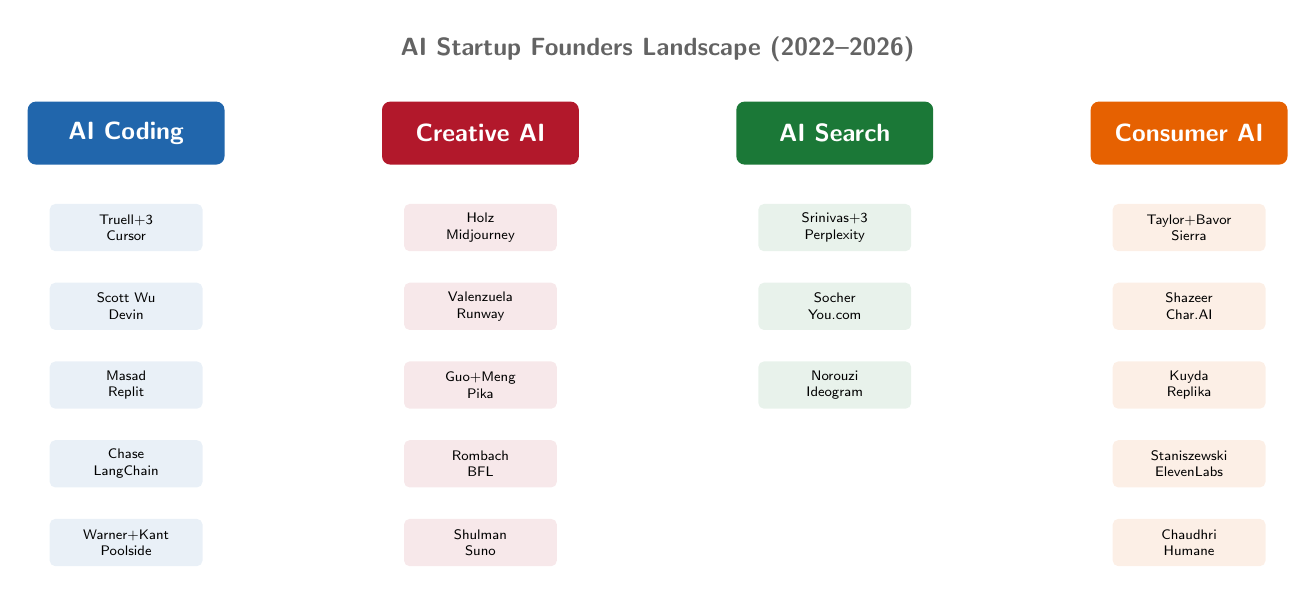
\begin{tikzpicture}[
  every node/.style={font=\sffamily},
  founder/.style={
    font=\sffamily\tiny, align=center, text width=1.8cm,
    rounded corners=2pt, inner sep=2pt, minimum height=0.6cm,
  },
  sector/.style={
    font=\sffamily\small\bfseries, text=white,
    rounded corners=3pt, inner sep=5pt, minimum height=0.8cm,
    minimum width=2.5cm,
  },
  arrow/.style={-{Stealth[length=3pt]}, figGray!50, thin},
]

% === Sector headers ===
\node[sector, fill=figBlue] (coding) at (0, 0) {AI Coding};
\node[sector, fill=figRed] (creative) at (4.5, 0) {Creative AI};
\node[sector, fill=figGreen] (search) at (9, 0) {AI Search};
\node[sector, fill=figOrange] (consumer) at (13.5, 0) {Consumer AI};

% === AI Coding founders ===
\node[founder, fill=figBlue!10] at (0, -1.2) {Truell+3\\Cursor};
\node[founder, fill=figBlue!10] at (0, -2.2) {Scott Wu\\Devin};
\node[founder, fill=figBlue!10] at (0, -3.2) {Masad\\Replit};
\node[founder, fill=figBlue!10] at (0, -4.2) {Chase\\LangChain};
\node[founder, fill=figBlue!10] at (0, -5.2) {Warner+Kant\\Poolside};

% === Creative AI founders ===
\node[founder, fill=figRed!10] at (4.5, -1.2) {Holz\\Midjourney};
\node[founder, fill=figRed!10] at (4.5, -2.2) {Valenzuela\\Runway};
\node[founder, fill=figRed!10] at (4.5, -3.2) {Guo+Meng\\Pika};
\node[founder, fill=figRed!10] at (4.5, -4.2) {Rombach\\BFL};
\node[founder, fill=figRed!10] at (4.5, -5.2) {Shulman\\Suno};

% === AI Search founders ===
\node[founder, fill=figGreen!10] at (9, -1.2) {Srinivas+3\\Perplexity};
\node[founder, fill=figGreen!10] at (9, -2.2) {Socher\\You.com};
\node[founder, fill=figGreen!10] at (9, -3.2) {Norouzi\\Ideogram};

% === Consumer AI founders ===
\node[founder, fill=figOrange!10] at (13.5, -1.2) {Taylor+Bavor\\Sierra};
\node[founder, fill=figOrange!10] at (13.5, -2.2) {Shazeer\\Char.AI};
\node[founder, fill=figOrange!10] at (13.5, -3.2) {Kuyda\\Replika};
\node[founder, fill=figOrange!10] at (13.5, -4.2) {Staniszewski\\ElevenLabs};
\node[founder, fill=figOrange!10] at (13.5, -5.2) {Chaudhri\\Humane};

% === Title ===
\node[font=\sffamily\small\bfseries, text=figGray, above=8pt] at (6.75, 0.5)
  {AI Startup Founders Landscape (2022--2026)};

\end{tikzpicture}
\caption{AI创业者版图：按赛道分布的代表性创始人。每个赛道都有其
独特的创始人画像——编程工具赛道以MIT/Harvard的年轻技术天才为主，
创意AI赛道跨越了艺术和科学的边界，搜索赛道以学术大牛为特征，
而消费AI赛道则汇聚了大厂高管和独立创新者。}
\label{fig:founders-landscape}
\end{figure}


% =============================================================
\section{本章人物索引}
\label{sec:founders-index}
% =============================================================

为便于查阅，以下按字母顺序列出本章提及的全部AI创业者。

\begin{keybox}[Chapter 11 人物索引]
\small
\begin{tabularx}{\textwidth}{l l X}
\toprule
\rowcolor{figLightGray}
\textbf{姓名} & \textbf{公司/产品} & \textbf{关键标签} \\
\midrule
Asif, Sualeh          & Cursor (Anysphere)   & MIT, CPO \\
Bavor, Clay           & Sierra AI            & ex-Google VP AR/VR, CTO \\
Blattmann, Andreas    & Black Forest Labs    & Stable Diffusion核心作者 \\
Bongiorno, Bethany    & Humane               & ex-Apple, AI Pin \\
Camacho, Martin       & Suno                 & 联合创始人, ex-Kensho \\
Chaudhri, Imran       & Humane               & ex-Apple 20年, AI Pin \\
Chase, Harrison       & LangChain            & Harvard, Agent框架 \\
Chen, Douglas         & Windsurf/Codeium     & 联合创始人, $\to$ Google \\
Crivello, Flo         & Lindy AI             & ex-Cruise, AI助手 \\
Dabkowski, Piotr      & ElevenLabs           & CTO, 波兰, 语音AI \\
De Freitas, Daniel    & Character.AI         & ex-Google LaMDA, $\to$ DeepMind \\
Dietzen, Scott        & Augment Code         & CEO, ex-Sun Microsystems \\
Ding, David           & Udio                 & CEO, ex-DeepMind \\
Esser, Patrick        & Black Forest Labs    & Stable Diffusion核心作者 \\
Friedman, Itamar      & Qodo (CodiumAI)      & CEO, 代码质量AI \\
Freyberg, Keenan      & Suno                 & 联合创始人, ex-Kensho \\
Garg, Div             & MultiOn              & CEO, 浏览器Agent \\
Germanidis, Anastasis & Runway               & 联合创始人, NYU Tisch \\
Guo, Demi             & Pika Labs            & CEO, Stanford PhD dropout \\
Gur-Ari, Guy          & Augment Code         & 创始人, ex-Google \\
Habib, May            & Writer               & CEO, 黎巴嫩裔加拿大人 \\
Hao, Steven           & Cognition (Devin)    & CTO, 竞赛编程 \\
Ho, Johnny            & Perplexity AI        & 联合创始人 \\
Holz, David           & Midjourney           & ex-Leap Motion, 无VC融资 \\
Hull, Chris           & Jasper AI            & 联合创始人 \\
Jain, Amit            & Luma AI              & CEO, Dream Machine \\
Kant, Eiso            & Poolside AI          & 联合创始人, ex-source\{d\} \\
Konwinski, Andy       & Perplexity AI        & 联合创始人, Apache Spark \\
Kucsko, Georg         & Suno                 & 联合创始人, ex-Kensho \\
Kuyda, Eugenia        & Replika              & CEO/创始人, AI伴侣先驱 \\
Liu, Beyang           & Sourcegraph          & CTO, Cody AI \\
Liu, Jerry            & LlamaIndex           & CEO, Princeton, RAG框架 \\
Lunnemark, Arvid      & Cursor (Anysphere)   & MIT, Jane Street \\
Lyu, Jesse (吕骋)     & Rabbit               & 西安$\to$硅谷, R1设备 \\
Masad, Amjad          & Replit               & 约旦$\to$硅谷, Replit Agent \\
Matamala, Alejandro   & Runway               & 联合创始人, 智利裔 \\
McCann, Bryan         & You.com              & 联合创始人, ex-Salesforce NLP \\
Meng, Chenlin         & Pika Labs            & CTO, Stanford PhD dropout \\
Mohan, Varun          & Windsurf/Codeium     & CEO $\to$ Google DeepMind \\
Morgan, John Philip   & Jasper AI            & 联合创始人 \\
Mostaque, Emad        & Stability AI         & 创始人, 2024年3月辞职 \\
Norouzi, Mohammad     & Ideogram             & 创始人, ex-Google Brain \\
Polu, Stanislas       & Dust                 & 创始人, ex-OpenAI \\
Rogenmoser, Dave      & Jasper AI            & CEO \\
Rombach, Robin        & Black Forest Labs    & Latent Diffusion发明者 \\
Sanger, Aman          & Cursor (Anysphere)   & MIT, COO \\
Shazeer, Noam         & Character.AI         & Transformer共同发明者 \\
Shulman, Mikey        & Suno                 & CEO, Harvard物理PhD \\
Socher, Richard       & You.com              & GloVe发明者, ex-Salesforce \\
Srinivas, Aravind     & Perplexity AI        & CEO, IIT Madras, ex-OpenAI \\
Staniszewski, Mati    & ElevenLabs           & CEO, 波兰, 语音AI \\
Taylor, Bret          & Sierra AI            & CEO, Google Maps共同创建者 \\
Truell, Michael       & Cursor (Anysphere)   & CEO, MIT, 25岁亿万富翁 \\
Valenzuela, Cristóbal & Runway               & CEO, 智利裔, NYU Tisch \\
Warner, Jason         & Poolside AI          & 联合创始人, ex-GitHub CTO \\
Wu, Scott             & Cognition (Devin)    & CEO, IOI金牌, Harvard \\
Yacoubian, Paul       & Copy.ai              & CEO, GTM AI \\
Yan, Walden           & Cognition (Devin)    & CPO, 竞赛编程 \\
Yarats, Denis         & Perplexity AI        & CTO, ex-Meta AI \\
\bottomrule
\end{tabularx}
\end{keybox}

\bigskip

本章覆盖的人物跨越了AI编程、搜索、创意生成、音乐/语音、Agent、消费
产品和硬件等多个赛道。他们的共同点是：在一个技术能力每6个月就翻倍的
时代，以惊人的速度将基础模型的能力转化为改变真实世界的产品。

在本书的其他章节中，读者将看到这些创业者与大型AI实验室
（第3--7章）、芯片和基础设施供应商（第9章）、投资者（第10章）和学术
研究者（第12章）之间千丝万缕的联系。AI创业不是一个孤立的现象，而是
整个AI生态系统共同演化的结果——大学培养人才，实验室推进技术，投资者
提供资本，而创业者则将这一切整合为\textbf{用户愿意付费的产品}。

对\textit{The AI Startup Landscape}读者的提示：本章与该书第5章
（开发者工具）、第7章（创意AI）和第9章（消费AI社交）形成直接对话。
\textit{Landscape}从\textbf{市场和产品}的角度分析这些公司，本章则
聚焦于\textbf{创始人}——他们是谁、从哪里来、为什么选择这条路。
两个视角互为补充。

\chapter{Enterprise AI, Vertical AI 与机器人革命}
\label{ch:enterprise}

%% ============================================================
%% Chapter 12: Enterprise AI, Vertical AI & Robotics Founders
%% Covers ~70 key figures across horizontal AI platforms,
%% vertical AI (legal, healthcare, finance, security, education,
%% sales, customer service), AI infrastructure/MLOps, and robotics.
%% ============================================================

当 ChatGPT 在 2022 年末引爆全球想象力时，
硅谷的一批创业者已经在思考一个更加务实的问题：
AI 如何真正改变每一个行业的工作方式？
消费级 AI 产品——聊天机器人、图像生成器、AI 伴侣——
吸引了绝大多数的公众注意力，
但在这道聚光灯之外，
一场规模更为宏大的变革正在企业世界的每一个角落悄然展开。

从华尔街的量化交易大厅到休斯顿的律师事务所，
从波士顿的肿瘤科诊室到匹兹堡的机器人实验室，
从旧金山的 MLOps 工具链到杭州的人形机器人工厂——
一群背景迥异的创始人正在将大语言模型、
计算机视觉和强化学习的前沿能力，
转化为解决特定行业痛点的商业产品。

他们中有 19 岁从 MIT 辍学创业的数据标注天才（Alexandr Wang），
有在 Google 管理百亿美元广告业务后转身投入 AI 搜索的高管（Sridhar Ramaswamy），
有在旧金山合租公寓里用 GPT-4 API 构建法律 AI 的室友搭档（Winston Weinberg 与 Gabriel Pereyra），
有在 CMU 机器人实验室里梦想``通用物理智能''的印度裔教授（Deepak Pathak 与 Abhinav Gupta），
有在华为``天才少年''计划中年薪百万后毅然辞职创业的 B 站 UP 主（彭志辉），
还有在 MIT 人工智能实验室完成博士论文后用四十年时间让机器人学会奔跑的传奇工程师（Marc Raibert）。

这些人的共同特征是：
他们不满足于 AI 作为一种``通用工具''的存在，
而是要将其深深嵌入特定行业的工作流、知识体系和决策链条之中。
这种``从通用到垂直''的转化能力，
正是当前 AI 产业最稀缺、也最具商业价值的能力。

\begin{keybox}[Enterprise AI 的核心公式：通用模型能力 $\times$ 行业知识深度 $\times$ 工作流嵌入度]
企业 AI 产品的成败取决于三个维度的乘积：
\begin{itemize}[noitemsep]
  \item \textbf{通用模型能力}——底层 LLM/视觉模型的推理、生成和理解能力。
        这是``地基''，决定了 AI 能做什么。
        GPT-4、Claude、Gemini 等模型的能力跃升，
        为所有企业 AI 应用提供了共同的技术底盘。
  \item \textbf{行业知识深度}——对特定领域术语、流程、合规要求和隐性知识的理解。
        这是``护城河''，决定了 AI 能做得多好。
        Harvey 理解判例法，Hippocratic AI 理解临床指南，
        CrowdStrike 理解 MITRE ATT\&CK 框架——
        这些行业知识无法通过简单的 prompt engineering 获得。
  \item \textbf{工作流嵌入度}——AI 是否真正嵌入了用户的日常工作流程，
        而非一个需要``额外切换''才能使用的独立工具。
        Gong 将 AI 嵌入销售团队的每一通电话，
        Viz.ai 将 AI 嵌入放射科医生的 CT 阅片流程，
        Scale AI 将数据标注嵌入 ML 团队的训练管线——
        这种``无缝嵌入''是 Enterprise AI 获得持续黏性的关键。
\end{itemize}
只有三者的乘积达到阈值，企业客户才会从``试用''走向``采购''，
从``单点部署''走向``全面推广''。
\end{keybox}

本章将按照``横向平台→垂直行业→基础设施→机器人''的逻辑，
系统介绍企业 AI 与机器人领域最具影响力的创始人群像。


%% ============================================================
\section{横向 AI 平台：数据、标注与企业智能}
\label{sec:ent-horizontal}
%% ============================================================

在企业 AI 生态系统中，
横向平台公司扮演着``基础设施供应商''的角色——
它们提供的不是面向某个特定行业的解决方案，
而是所有 AI 应用都需要的通用能力：
数据标注、模型训练基础设施、实验追踪、数据仓库、可观测性。
这些公司的创始人往往具有深厚的系统工程或分布式计算背景，
他们构建的是 AI 产业的``水和电''。

%% ------------------------------------------------------------
\subsection{Alexandr Wang 与 Scale AI：数据基础设施的定义者}
\label{subsec:alexandr-wang}
%% ------------------------------------------------------------

在整个 AI 产业的价值链中，
有一个环节长期被低估却又不可或缺——\textbf{数据标注}。
每一个让人惊叹的 AI 模型背后，
都有海量的人工标注数据作为训练的燃料。
识别这个机会并将其转化为一家市值数百亿美元公司的人，
是一个 1997 年出生在新墨西哥州 Los Alamos 的华裔美国人——
Alexandr Wang（汪滔）。

\begin{corebox}[Alexandr Wang：从物理学家之子到 AI 时代的数据之王]
\textbf{出生}：1997 年 1 月，美国新墨西哥州 Los Alamos\\
\textbf{教育}：MIT（辍学）\\
\textbf{父母}：均为 Los Alamos 国家实验室核物理学家（中国移民）\\
\textbf{早期经历}：2012 年 USACO 决赛选手，2013 年数学奥林匹克项目，
2014 年美国物理代表队；高中时期在 Quora 担任技术负责人\\
\textbf{创业}：2016 年从 MIT 辍学，经 Y Combinator 孵化，
与 Lucy Guo 共同创立 Scale AI\\
\textbf{里程碑}：2021 年以 24 岁成为世界最年轻白手起家亿万富翁（Forbes 估值 36 亿美元，2025 年 4 月）\\
\textbf{现职}：2025 年起担任 Meta Platforms 首席 AI 官，
领导其 Superintelligence Labs
\end{corebox}

Wang 的创业故事始于一个看似``无聊''却无比关键的洞察：
AI 模型的质量上限由训练数据的质量决定，
而高质量数据标注是整个 AI 产业链中最大的瓶颈。
2016 年，当大多数 AI 创业者都在追逐``模型创新''时，
19 岁的 Wang 选择了一条截然不同的路径——
成为 AI 时代的``数据基础设施供应商''。

Scale AI 最初的产品极其朴素：
通过 API 接口接受客户的数据标注任务（图像分类、物体检测、语义分割等），
再将任务分发给全球的标注员完成。
但 Wang 的野心远不止于``众包标注''——
他要构建的是一个\textbf{数据质量控制的技术栈}，
通过算法辅助、多轮审核、标注员能力建模等手段，
确保标注数据的准确率和一致性达到机器学习研究级别的标准。

这个战略定位在 2020--2023 年的 AI 军备竞赛中被证明极具前瞻性。
当 OpenAI、Anthropic、Google、Meta 等公司竞相训练更大的模型时，
它们都需要 Scale AI 提供的高质量标注数据——
特别是在 RLHF（基于人类反馈的强化学习）这一关键训练范式中，
Scale AI 的标注质量直接影响模型的对齐效果。

\begin{whybox}[为什么 Scale AI 能成为 AI 产业的``隐形冠军''？]
Scale AI 的竞争优势建立在三个飞轮之上：
\begin{enumerate}[noitemsep]
  \item \textbf{客户网络效应}：服务 OpenAI、Meta、美国国防部等顶级客户，
        积累了对最前沿 AI 训练需求的第一手理解，
        反过来驱动产品迭代。
  \item \textbf{标注员生态}：建立了全球最大的高质量标注员网络，
        涵盖从通用任务到专业领域（医学影像、法律文本、代码）的多层次人才池。
  \item \textbf{从标注到评估的扩展}：随着模型能力提升，
        ``评估模型输出质量''（evaluation）成为新的刚需，
        Scale AI 从数据标注自然延伸到 LLM 评估（benchmarking），
        推出了广受行业认可的 SEAL Leaderboard。
\end{enumerate}
\end{whybox}

Wang 的政策影响力同样不容忽视。
2025 年 1 月，Scale AI 在《华盛顿邮报》刊登整版广告，
发表致 Trump 总统的公开信：``America must win the AI War''。
同月，Wang 在国会作证，
警告中国 AI 公司已经在多个领域追平美国竞争对手，
呼吁政府加大对 AI 产业的支持力度。
这种``技术创业者+政策倡导者''的双重身份，
使 Wang 成为 AI 时代华裔创业者中最具公共影响力的面孔之一。

2025 年，Wang 做出了一个令人意外的职业转向——
加入 Meta Platforms 担任首席 AI 官，
领导新成立的 Superintelligence Labs。
这一任命的信号意义在于：
连 Zuckerberg 都认为，
在 AI 竞赛的下一个阶段，
\textbf{数据}和\textbf{评估}的重要性不亚于模型本身。


%% ------------------------------------------------------------
\subsection{Ali Ghodsi 与 Databricks：从学术论文到 620 亿美元帝国}
\label{subsec:ali-ghodsi}
%% ------------------------------------------------------------

如果说 Scale AI 定义了``AI 的数据标注层''，
那么 \textbf{Databricks} 则定义了``AI 的数据处理层''。
这家公司的故事，是学术研究如何转化为商业帝国的经典范本——
也是一个``意外创业''的传奇。

\begin{corebox}[Ali Ghodsi：从伊朗到伯克利，从教授到 CEO]
\textbf{出生}：1978 年，伊朗\\
\textbf{国籍}：瑞典-美国双重国籍\\
\textbf{教育}：KTH 皇家理工学院（博士，分布式系统），Mid Sweden University（硕士+MBA）\\
\textbf{学术经历}：KTH 助理教授（2008--2009），
UC Berkeley 访问学者（2009 年起），
与 Scott Shenker、Ion Stoica、Michael Franklin、Matei Zaharia 合作\\
\textbf{核心贡献}：参与创建 Apache Mesos、Apache Spark 项目；
共同发明 Dominant Resource Fairness 资源调度算法\\
\textbf{创业}：2013 年共同创立 Databricks，2016 年出任 CEO\\
\textbf{估值}：2025 年 620 亿美元（私有公司）
\end{corebox}

Databricks 的创立故事堪称硅谷``学术创业''的典范。
2009 年，Ghodsi 从瑞典来到 UC Berkeley 做访问学者，
与 Ion Stoica 实验室的一群博士生——
包括 Matei Zaharia（Apache Spark 的发明人）——
一起研究分布式计算系统。
Spark 最初只是一篇学术论文中的原型系统，
用于解决 Hadoop MapReduce 在迭代计算中的性能瓶颈。

2013 年，七位 Berkeley 研究者联合创立了 Databricks，
试图将 Spark 商业化。
但早期发展异常艰难——
用 Forbes 的话说，这是一家``long on buzz but short on revenue''的公司。
到 2015 年 11 月，公司已经花了五个月时间试图融资却处处碰壁，
投资人对其微薄的营收心存疑虑。
NEA 合伙人 Pete Sonsini 不得不以紧急注资 3000 万美元的方式拯救公司。

转折出现在 Ghodsi 接任 CEO 之后。
不同于竞争对手 Snowflake 两次引入硅谷职业经理人的做法，
Databricks 选择了``学术创始人自己来''的道路。
Ghodsi 展现出了罕见的``学者型 CEO''能力——
既能理解分布式系统的深层技术，
又能将其翻译为企业客户听得懂的商业语言。
在他的领导下，Databricks 从一个``Spark 商业化''公司
转型为统一的``数据+AI 平台''（Data Intelligence Platform），
将数据仓库、数据湖、机器学习、实时分析整合在一个平台上。

到 2025 年，Databricks 的估值已达 620 亿美元，
成为全球估值最高的 AI 基础设施私有公司之一。

\begin{whybox}[Databricks 的七位联合创始人与伯克利 AMPLab 传奇]
Databricks 的七位联合创始人全部来自 UC Berkeley 的 AMPLab，
这是硅谷历史上最成功的大学实验室创业案例之一：
\begin{itemize}[noitemsep]
  \item \textbf{Ion Stoica}——教授，初任 CEO（后回到 Berkeley），同时也是 Anyscale 联合创始人
  \item \textbf{Matei Zaharia}——Apache Spark 发明人，CTO
  \item \textbf{Ali Ghodsi}——现任 CEO
  \item \textbf{Patrick Wendell}——Spark 核心贡献者
  \item \textbf{Reynold Xin}——Spark SQL 主要作者
  \item \textbf{Andy Konwinski}——Mesos 贡献者
  \item \textbf{Arsalan Tavakoli}——基础设施专家
\end{itemize}
这种``整个实验室集体创业''的模式，
确保了公司在技术深度上的绝对优势——
七位创始人是 Spark、Mesos、Delta Lake 等核心技术的原始发明人，
没有任何竞争对手能复制这种``从论文到产品''的技术纵深。
\end{whybox}


%% ------------------------------------------------------------
\subsection{Sridhar Ramaswamy 与 Snowflake：Google 高管的 AI 转身}
\label{subsec:sridhar-ramaswamy}
%% ------------------------------------------------------------

如果 Ali Ghodsi 代表的是``学术创始人''路径，
那么 \textbf{Sridhar Ramaswamy} 则代表了另一种创业轨迹——
\textbf{大公司高管的``二次创业''转型}。

Ramaswamy 在 Google 工作了 15 年（2003--2018），
最终升至 Google 广告业务的高级副总裁，
直接管理着年收入超过 1000 亿美元的广告帝国。
2018 年，他离开 Google，
原因据他自己所说是对广告业务模式产生了``道德上的不安''——
他开始质疑``以用户注意力为商品''的商业逻辑是否可持续。

离开 Google 后，Ramaswamy 创立了 \textbf{Neeva}，
一个无广告的 AI 驱动搜索引擎。
Neeva 的愿景很美好——
用订阅制替代广告模式，用 AI 替代传统搜索排名——
但在 Google 搜索的垄断面前，
一个付费搜索引擎实在难以获得大规模用户。
2023 年 5 月，Neeva 宣布关闭消费者搜索业务。

然而，失败的 Neeva 意外地成为了通往更大舞台的跳板。
2023 年，Snowflake 以未披露的价格收购了 Neeva 的团队和技术，
Ramaswamy 加入 Snowflake 担任 AI 高级副总裁。
仅仅几个月后的 2024 年 2 月 28 日，
传奇 CEO Frank Slootman 宣布退休，
Ramaswamy 被任命为 Snowflake 新任 CEO。

这一任命的信号极为明确：
Snowflake 的董事会认为，在 AI 重塑数据产业的关键时刻，
公司需要一位\textbf{深度理解 AI 技术}的领导者，
而非传统的企业软件销售型 CEO。
Ramaswamy 上任后，迅速将 Snowflake 从``云数据仓库''
重新定位为``AI 数据云''（AI Data Cloud），
推出了 Cortex AI（企业级 AI/ML 平台）、
Arctic（Snowflake 自研的开源 LLM）等一系列 AI 产品。


%% ------------------------------------------------------------
\subsection{Lukas Biewald 与 Weights \& Biases：ML 实验的``版本控制''}
\label{subsec:lukas-biewald}
%% ------------------------------------------------------------

在机器学习的日常工作中，
有一个痛点长期被忽视：\textbf{实验管理}。
一个 ML 工程师在一天之内可能训练数十个模型变体，
每个变体的超参数、数据集、指标、模型权重都不同。
如何系统地追踪、比较和复现这些实验？

\textbf{Lukas Biewald} 正是解决这个问题的人。
Biewald 的创业生涯始于 2007 年创立的 Figure Eight（前身为 CrowdFlower），
一家众包数据标注公司——
比 Scale AI 早了近十年。
Figure Eight 在 2019 年被 Appen 收购后，
Biewald 在 2018 年联合创立了 \textbf{Weights \& Biases}（简称 W\&B/wandb），
专注于 ML 实验追踪和模型管理。

W\&B 的核心产品看似简单——
在训练脚本中加几行代码，
就能自动记录每次实验的所有元数据（超参数、损失曲线、GPU 利用率、模型权重），
并提供直观的 Web 界面进行可视化和比较。
但正是这种``简单到令人上瘾''的开发者体验，
使 W\&B 成为了 ML 社区中渗透率最高的工具之一——
从 OpenAI 到 DeepMind，从学术实验室到初创公司，
几乎所有认真做 ML 的团队都在使用 W\&B。

2025 年 10 月，W\&B 被 CoreWeave 收购，
Biewald 继续担任 W\&B 的总经理。
这笔收购的逻辑在于：
CoreWeave 作为 GPU 云计算提供商，
通过收购 W\&B 可以为客户提供``从计算到实验管理''的端到端体验。


%% ------------------------------------------------------------
\subsection{Alex Karp 与 Palantir：从反恐到 AI 平台}
\label{subsec:alex-karp}
%% ------------------------------------------------------------

在企业 AI 的版图中，
\textbf{Palantir} 是一个极其特殊的存在——
它既不是典型的 SaaS 公司，也不是纯粹的 AI 初创企业，
而是一家拥有二十余年历史、
从反恐情报分析起家的数据分析公司，
在 AI 时代完成了一次令人瞩目的``蜕变''。

\textbf{Alex Karp}，Palantir 的联合创始人兼 CEO，
是硅谷最不像 CEO 的 CEO。
他是哲学博士（法兰克福大学，师从 Jürgen Habermas），
没有工程背景，性格古怪，
曾公开承认自己``不会写代码''。
但正是这个``哲学家 CEO''，
带领 Palantir 完成了 AI 时代最成功的战略转型之一。

2023 年，Palantir 推出了 \textbf{AIP}（Artificial Intelligence Platform），
将大语言模型的能力直接嵌入其 Foundry 和 Gotham 平台。
AIP 的核心创新在于``本体论驱动的 AI 部署''——
企业无需从零构建 AI 应用，
而是将 LLM 的能力``绑定''到已有的数据模型和业务逻辑之上。
这种方法极大地降低了企业部署 AI 的门槛和风险。

AIP 的推出引发了 Palantir 股价的爆发性增长。
2025 年第四季度，Palantir 报告了 70\% 的同比收入增长，
达到 14.07 亿美元；
美国业务更是增长了 93\%。
Karp 在财报电话会上说了一句令人印象深刻的话：
``AI has just put gasoline on all the tribal knowledge we have in our products.''

\begin{whybox}[Palantir 的 AI 转型为何如此成功？]
Palantir 的 AI 转型成功有三个结构性原因：
\begin{enumerate}[noitemsep]
  \item \textbf{数据层的先发优势}：二十年来，Palantir 一直在帮助政府和企业
        整理、清洗和结构化它们最混乱的数据。当 LLM 需要结构化数据才能发挥最大价值时，
        Palantir 的客户已经拥有了``AI-ready''的数据基础。
  \item \textbf{安全与合规的护城河}：Palantir 拥有最高级别的政府安全认证，
        能在 classified 环境中部署 AI——这是 OpenAI 和 Google 都难以进入的领域。
  \item \textbf{收入质量的跃升}：Karp 指出，增长主要来自现有客户的支出增加，
        而非新客户数量的增长。这意味着 AI 功能使 Palantir
        从``nice-to-have''变成了``mission-critical''。
\end{enumerate}
\end{whybox}


%% ------------------------------------------------------------
\subsection{Olivier Pomel 与 Datadog：可观测性遇上 AI}
\label{subsec:olivier-pomel}
%% ------------------------------------------------------------

在 AI 应用爆炸式增长的时代，
一个容易被忽视但至关重要的问题是：
\textbf{如何监控和调试 AI 系统？}
传统的软件监控工具是为确定性系统设计的——
服务器要么正常运行，要么宕机。
但 AI 系统的``故障''模式完全不同——
模型可能在运行，但输出质量在悄然退化（model drift）；
LLM 可能在响应，但成本在不知不觉中飙升。

\textbf{Datadog} 的联合创始人兼 CEO \textbf{Olivier Pomel}
正在将公司从传统的``云基础设施可观测性''
扩展为``AI 时代的全栈可观测性''。
Pomel 是法国裔美国人，
在创立 Datadog 之前曾在几家纽约科技公司工作。
2010 年，他与 Alexis Lê-Quôc 共同创立 Datadog，
最初专注于云基础设施监控。

到 2025--2026 年，Datadog 已经推出了一整套 AI 监控产品：
\textbf{LLM Observability}（追踪 LLM 调用的延迟、成本、token 使用量和输出质量）、
\textbf{Bits AI}（AI 驱动的运维助手，能自动分析告警并提供修复建议）、
以及 \textbf{Toto}（Datadog 自研的基础模型，专门用于理解运维数据）。
Pomel 将公司的长期战略描述为``race against complexity''——
AI 正在使软件系统变得更复杂、更快速地变化，
而 Datadog 要确保企业能够``看清''这些变化。


%% ============================================================
\section{垂直 AI：行业深水区的变革者}
\label{sec:ent-vertical}
%% ============================================================

如果说横向平台公司是 AI 时代的``水和电''，
那么垂直 AI 公司就是将这些基础能力转化为
行业特定价值的``应用工厂''。
这些公司的创始人通常具有双重背景——
既懂 AI 技术，又深谙目标行业的痛点和工作流。
这种``跨界能力''是垂直 AI 创业最稀缺的资源。


%% ============================================================
\subsection{AI for Legal：当 GPT-4 遇见判例法}
\label{subsec:legal-ai}
%% ============================================================

法律行业是企业 AI 渗透最快、商业化最成功的垂直领域之一。
原因很简单：法律工作的核心是处理文本——
合同、判例、法规、诉讼文书——
而这正是大语言模型最擅长的领域。
同时，法律服务的定价极高（大型律所合伙人时薪可达 1000--2000 美元），
任何能提高效率的工具都有立竿见影的 ROI。

\subsubsection{Harvey AI：从合租室友到 80 亿美元法律帝国}

在所有法律 AI 公司中，
\textbf{Harvey} 的崛起速度最为惊人——
从 2022 年创立到 2025 年估值 80 亿美元，只用了三年。
更令人惊叹的是它的收入增长轨迹：
2025 年 8 月，Harvey 宣布其年化经常性收入（ARR）突破 1 亿美元，
创立仅 36 个月便达到这一里程碑——
作为对比，Salesforce 花了 7 年，Slack 花了 4 年，
甚至 Zoom 也用了 42 个月。

Harvey 的两位创始人——\textbf{Gabriel Pereyra} 和 \textbf{Winston Weinberg}——
是一对极为互补的搭档。

\begin{corebox}[Harvey AI 的``室友创始人''组合]
\textbf{Gabriel Pereyra}（总裁，31 岁）：
AI 研究科学家，曾在 DeepMind 和 Meta 从事 AI 研究。
关键优势是在 ChatGPT 公开发布前六个月，
就获得了 GPT-4 的早期访问权限——
这使他比几乎所有竞争对手都更早看到了 LLM 在法律场景中的潜力。

\textbf{Winston Weinberg}（CEO，28 岁）：
Kenyon College 本科，USC Gould 法学院 JD。
曾在 O'Melveny \& Myers 律所担任一年级诉讼律师——
这段短暂的 BigLaw 经历使他深刻理解了
法律工作中哪些痛点是 AI 可以真正解决的。

两人在旧金山合租公寓时决定一起创业。
截至 2026 年初，尽管公司估值已达 80 亿美元，
两人仍然住在同一间公寓里。
\end{corebox}

Harvey 的成功有一个关键转折点：
2023 年初，全球``魔法圈''律所 \textbf{Allen \& Overy}
成为 Harvey 的第一个大型客户。
这一合作在极度保守的法律行业引发了多米诺效应——
当 Allen \& Overy 这样的顶级律所都开始使用 AI 时，
其他律所面临着``不用就落后''的竞争压力。
到 2025 年底，Harvey 已服务超过 1000 家律所和企业法务部门，
覆盖 63 个国家，包括 42\% 的 AmLaw 100 律所。

Harvey 的技术策略也值得关注：
它不是一个简单的``GPT-4 套壳''产品，
而是构建了一个完整的法律 AI 基础设施——
从合同起草到监管分析，从尽职调查到诉讼准备，
覆盖法律工作的全流程。
Pereyra 将 Harvey 定位为法律行业的``AI 操作系统''，
而非单一功能工具。

\subsubsection{Jake Heller 与 Casetext：被收购的先驱}

在 Harvey 之前，\textbf{Casetext} 是法律 AI 领域最重要的先行者。
2013 年由 \textbf{Jake Heller} 创立的 Casetext，
早在 GPT-4 发布之前就开始探索如何将 AI 应用于法律研究。
2023 年初，Casetext 成为最早基于 GPT-4 构建产品的公司之一，
推出了 \textbf{CoCounsel}——一个能在几分钟内完成
文档审查、法律研究备忘录、证词准备和合同分析的 AI 法律助手。

CoCounsel 的产品质量引起了 Thomson Reuters 的注意。
2023 年 6 月，Thomson Reuters 宣布以 6.5 亿美元收购 Casetext——
这是生成式 AI 时代法律科技领域最大的收购案之一。
到 2026 年 2 月，CoCounsel 已拥有超过 100 万专业用户，
标志着法律 AI 从``试点''阶段正式进入``大规模生产''阶段。

\subsubsection{EvenUp：AI 赋能人身伤害诉讼}

与 Harvey 专注大型律所不同，
\textbf{EvenUp} 瞄准的是一个更``接地气''的市场——\textbf{人身伤害诉讼}。
联合创始人 \textbf{Raymond Mieszaniec} 的背景颇为独特：
他曾在 PwC 香港和中国的风险咨询部门工作，
涉及分析、网络安全、金融犯罪和合规领域，
之后联合创立了 EquitySim（一个 AI 驱动的模拟招聘平台）。

EvenUp 的核心产品是利用机器学习自动生成``索赔要求书''（demand package）——
在人身伤害案件中，这是律师向保险公司提出赔偿要求的关键文档。
传统上，一份高质量的索赔要求书需要律师花费数小时甚至数天来整理
医疗记录、评估案件价值、撰写论证。
EvenUp 将这个过程压缩到分钟级别。

2025 年 10 月，EvenUp 完成了 1.5 亿美元的 E 轮融资，
估值突破 20 亿美元。


%% ============================================================
\subsection{AI for Healthcare：生死攸关的精准医疗}
\label{subsec:healthcare-ai}
%% ============================================================

医疗健康是 AI 应用最具社会影响力、
但也最难商业化的垂直领域。
监管壁垒（FDA 审批）、数据隐私（HIPAA）、
临床验证要求和极高的安全标准，
共同构成了一道``护城河''——
既保护了先行者，也阻挡了后来者。

\subsubsection{Munjal Shah 与 Hippocratic AI：让 AI 说``首先，不要伤害''}

\textbf{Munjal Shah} 是一位连续创业者中的``老将''。
在创立 Hippocratic AI 之前，
他已经成功创立并出售了三家公司：
\textbf{Andale}（被 Vendio 收购）、
\textbf{Riya}（人脸识别先驱，技术转型为 Like.com），
以及 \textbf{Like.com}（视觉搜索引擎，2010 年被 Google 以超过 1 亿美元收购）。
Like.com 的收购尤为值得一提——
它证明了 Shah 在 AI 领域的直觉：
当面部识别的消费者市场时机不成熟时，
他果断将同一技术转向了电商视觉搜索。

2023 年，Shah 创立了 \textbf{Hippocratic AI}，
公司名称直接取自希波克拉底誓言——
``首先，不要伤害''（First, do no harm）。
Hippocratic AI 的定位极为精准：
不做诊断（这是监管雷区），
而是专注于\textbf{非诊断性}的医疗任务——
慢性病管理、出院后随访、药物提醒、营养咨询、患者导航。

其核心技术是 \textbf{Polaris} 架构——
一个多智能体 LLM 系统，
专门优化用于实时医疗对话。
每个 AI Agent 在发布前都经过与美国执业护士和患者演员的
大规模模拟对话测试，确保临床安全性。

Hippocratic AI 的融资轨迹极其陡峭：
2024 年 4 月 A 轮 5300 万美元（估值 5 亿），
2025 年 1 月 B 轮 1.41 亿美元（估值 16.4 亿），
2025 年 11 月 C 轮 1.26 亿美元（估值 35 亿），
总融资额达 4.04 亿美元。
投资人包括 a16z、Kleiner Perkins、NVIDIA、General Catalyst、
Google CapitalG 等顶级机构。

\subsubsection{Thomas Fuchs 与 Paige AI：计算病理学的先驱}

\textbf{Thomas Fuchs} 的人生轨迹跨越了太空与医学。
在进入医疗 AI 领域之前，
他曾在 NASA 的喷气推进实验室（JPL）担任工程师，
参与火星探测相关的计算机视觉研究。
这段在太空领域的经历塑造了他处理高风险、
高精度视觉任务的方法论。

2017 年，Fuchs 联合创立了 \textbf{Paige}，
专注于\textbf{计算病理学}——
利用 AI 分析组织切片的数字化图像来辅助癌症诊断。
Paige 创造了历史：它是\textbf{第一家获得 FDA 批准}
用于癌症诊断的 AI 工具的公司。
Fuchs 同时担任 Icahn School of Medicine at Mount Sinai
的人工智能和人类健康学院院长，
这种``学术+工业''的双重身份使 Paige
能够持续获取最新的临床研究成果。

\subsubsection{Eric Lefkofsky 与 Tempus AI：从 Groupon 到精准医疗}

\textbf{Eric Lefkofsky} 可能是本章中背景最``反差''的创始人之一。
他最广为人知的身份是 \textbf{Groupon} 的联合创始人——
那个 2010 年代初期红极一时、
后来却成为``团购泡沫''代名词的公司。

但 Lefkofsky 的第二次创业却完全不同。
2015 年，他创立了 \textbf{Tempus AI}，
目标是构建\textbf{世界上最大的分子和临床数据库}，
以及一个使这些数据可访问、可用于精准医疗的操作系统。
Tempus 的核心价值在于：
它将基因组测序数据与临床治疗结果关联起来，
帮助医生根据每个患者的分子特征做出最优的治疗决策。

2024 年 6 月，Tempus AI 成功 IPO，
以每股 37 美元的价格筹集了 4.11 亿美元，
完全稀释后市值超过 60 亿美元。

\subsubsection{Chris Mansi 与 Viz.ai：每一分钟都是生命}

对于中风患者来说，\textbf{时间就是大脑}——
每延误一分钟治疗，患者平均损失 190 万个神经元和 140 亿个突触；
每延误 10 分钟，等于失去 8 周的寿命。

\textbf{Chris Mansi} 博士曾是英国的一名神经外科医生，
亲身经历过中风治疗中每一分钟浪费在低效流程上
带来的灾难性后果。
2016 年，他创立了 \textbf{Viz.ai}，
利用 AI 实时分析 CT 扫描图像，
检测大血管闭塞（LVO）中风的早期迹象，
并立即通过手机通知主治医生——
将诊断时间从数小时缩短到数分钟。

2024 年，Mansi 被 TIME 杂志评为
``TIME100 AI''——全球 100 位最具影响力的 AI 人物之一。

\subsubsection{Chris Gibson 与 Recursion Pharmaceuticals：AI 驱动的新药发现}

\textbf{Chris Gibson} 博士在 2013 年联合创立了 \textbf{Recursion Pharmaceuticals}，
带着一个大胆的承诺：``用 10 年时间开发 100 种药物。''
Recursion 的方法是将高通量实验与 AI 结合——
自动化地对大量细胞进行药物处理，
用显微镜捕捉细胞形态变化的图像，
再用 AI 从海量图像中发现人类肉眼无法识别的规律。

12 年过去了，Recursion 尚未将任何药物推向市场，
也在 2025 年砍掉了近一半的产品管线。
但公司仍然签下了价值超过 200 亿美元的大药企合作协议
（包括 Roche、Bayer、Sanofi、Merck KGaA），
产生了 5 亿美元的合作收入。
2024 年，Recursion 以 6.88 亿美元收购了英国 AI 制药公司 Exscientia，
巩固了其在 TechBio 领域的领先地位。
2025 年 11 月，Gibson 宣布卸任 CEO，转任董事长，
将日常运营交给新任 CEO Najat Khan。


%% ============================================================
\subsection{AI for Finance：华尔街的算法革命}
\label{subsec:finance-ai}
%% ============================================================

华尔街对 AI 的拥抱比大多数行业更早、更深。
量化交易基金从 1990 年代就开始使用统计模型和机器学习，
而 LLM 的出现又打开了新的可能性——
从自动化研究报告生成到实时市场情绪分析。

\subsubsection{David Siegel 与 Two Sigma：量化投资的 AI 先驱}

\textbf{David Siegel}（1961 年生，纽约布朗克斯）
是一位早慧的计算机科学家。
12 岁时，他就在纽约大学 Courant 数学研究所的超级计算机上学习编程。
在 Princeton 大学获得电气工程学位后，
他在 MIT 人工智能实验室完成了计算机科学博士学位。

2001 年，Siegel 与 John Overdeck 联合创立了 \textbf{Two Sigma}，
核心理念是：``通过创新技术和数据科学发现世界数据中的价值。''
这在 2001 年是一个极具前瞻性的愿景——
当时``大数据''这个词还不存在，
``机器学习''还是学术论文中的术语。

二十多年后，Two Sigma 管理着约 580 亿美元的资产，
是全球最大的量化对冲基金之一。
在 AI 时代，Two Sigma 进一步加大了对 LLM 的投入——
利用 LLM 分析财报电话会议、SEC 文件、新闻报道和社交媒体，
提取交易信号。
公司的数据科学团队正在探索如何将
Alternative Data（另类数据）与 LLM 结合，
为量化策略和主观投资都创造超额收益（alpha）。


%% ============================================================
\subsection{AI for Customer Service：客服行业的``iPhone 时刻''}
\label{subsec:customer-service-ai}
%% ============================================================

客户服务是 AI 最早、最成功地实现商业化的垂直领域。
原因很直观：客服工作的核心是``理解问题+给出答案''，
这正是 LLM 最擅长的任务模式。
2024--2025 年，AI 客服从``辅助人类客服''
迅速演进为``自主解决问题的 AI Agent''，
掀起了一场深刻的行业变革。

\subsubsection{Bret Taylor 与 Clay Bavor：Sierra AI 的``梦之队''}

在 AI 客服领域，\textbf{Sierra AI} 的两位联合创始人
可能拥有科技行业中最耀眼的简历组合。

\begin{corebox}[Sierra AI：硅谷``全明星''的再次出发]
\textbf{Bret Taylor}（联合创始人兼 CEO）：
\begin{itemize}[noitemsep]
  \item Google Maps 的共同创造者（Google 最早一批 APM）
  \item FriendFeed 创始人（被 Facebook 收购，Taylor 出任 Facebook CTO）
  \item Quip 创始人（被 Salesforce 以 7.5 亿美元收购）
  \item Salesforce Co-CEO（2021--2023）
  \item Twitter/X 董事会主席（2022）
  \item \textbf{OpenAI 董事会主席}（现任）
\end{itemize}

\textbf{Clay Bavor}（联合创始人兼总裁）：
\begin{itemize}[noitemsep]
  \item 在 Google 工作超过 18 年
  \item 与 Taylor 同期加入 Google APM 项目
  \item 先后负责 Gmail、Google Drive、Google Docs 等核心产品
  \item 领导 Google Labs 和 AR/VR 团队
\end{itemize}
\end{corebox}

Sierra 的创立故事颇为浪漫。
2023 年 1 月，Taylor 从 Salesforce Co-CEO 的职位辞职。
``辞职消息发出的那一刻，''Taylor 回忆道，
``我就接到了一个老朋友的电话，邀我出去吃午饭。''
这个老朋友就是 Bavor。
两人在 Palo Alto 一家地中海餐厅里
一边喝草本茶一边聊了几个小时——
出门时，他们已经决定一起创业。

Sierra 专注于帮助企业构建客户服务 AI Agent。
与通用聊天机器人不同，Sierra 的 Agent 被设计为
能够理解每个企业的特定业务逻辑、产品目录和服务政策，
并能够在对话中\textbf{执行实际操作}——
处理退款、修改订单、更新账户信息——
而不仅仅是``回答问题''。

2025 年 9 月，Sierra 完成了 3.5 亿美元的融资，
估值达到 100 亿美元。
公司声称已拥有数百家客户，
包括 SoFi、Ramp、Brex 等知名金融科技公司。
截至目前，Sierra 的总融资额已达 6.35 亿美元。

\subsubsection{Eoghan McCabe 与 Intercom：传统客服软件的 AI 重生}

如果 Sierra 代表的是``AI 原生''的新进入者，
那么 \textbf{Intercom} 则代表了``传统客服软件公司的 AI 转型''路径。

\textbf{Eoghan McCabe}，Intercom 的联合创始人兼 CEO，
是爱尔兰裔连续创业者。
Intercom 成立于 2011 年，最初是一个面向互联网企业的
客户沟通平台——在线聊天、产品内消息、帮助中心。
在 AI 浪潮到来之前，
Intercom 已经是 SaaS 客服领域的头部玩家。

2023 年，McCabe 做出了一个大胆的决定：
将 Intercom 的整个产品战略围绕 AI 进行重构。
公司推出了 \textbf{Fin}——一个基于 LLM 的 AI 客服 Agent。
Fin 的表现超出了几乎所有人的预期：
平均解决率达到 67\%（即三分之二的客户问题由 AI 自主解决），
每周解决近 200 万个客户问题。

到 2026 年初，Fin 已拥有 8000 个客户，
收入接近 1 亿美元。
更令人印象深刻的是其客户名单——
包括 Anthropic、Snowflake 和 Polymarket。
2026 年 3 月，Intercom 从 Hercules Capital 获得了 2.5 亿美元的债务融资，
McCabe 选择债务而非股权融资的原因是``避免对股东的稀释''——
这一融资策略本身就说明了 Fin 的收入质量之高。

\subsubsection{Jesse Zhang 与 Ashwin Sreenivas：Decagon 的年轻挑战者}

在 Sierra 和 Intercom 之间，
一家更年轻的公司正在快速崛起——
\textbf{Decagon}，由 28 岁的 \textbf{Jesse Zhang}
和 \textbf{Ashwin Sreenivas} 联合创立。

Decagon 的差异化在于其对``企业级''的执着追求——
它不仅是一个聊天机器人，
而是一个能够横跨语音、聊天、邮件、短信等所有客户渠道的
AI Agent 平台。
客户包括 Avis Budget Group、Chime、Oura Health、1-800-FLOWERS 和 Hunter Douglas
等知名企业。

2024 年 10 月，Decagon 完成了 6500 万美元的 B 轮融资
（由 Bain Capital Ventures 领投），
总融资额达到 1 亿美元，估值在几个月内翻了四倍。

\subsubsection{Deon Nicholas 与 Forethought：加拿大天才的 AI 客服梦}

\textbf{Deon Nicholas} 是一位加拿大裔创业者，
曾在 Facebook、Palantir、Dropbox 和 Pure Storage 等公司工作，
持有机器学习相关专利，
曾是 ACM 国际大学生编程竞赛（ICPC）的全球总决赛选手。

2017 年，Nicholas 创立了 \textbf{Forethought}，
专注于利用 AI 自动化客户支持。
在 LLM 爆发之前，
Forethought 就已经在用自然语言处理技术
实现工单分类、知识库搜索和自动回复。
LLM 的出现为其产品能力带来了质的飞跃——
Forethought 的 AI Agent 不仅能回答问题，
还能自动执行操作（如退款、密码重置）和跟进未解决的工单。
Nicholas 被 Forbes 评为``30 Under 30''，
公司累计融资超过 9200 万美元。


%% ============================================================
\subsection{AI for Sales \& Marketing：收入增长的 AI 引擎}
\label{subsec:sales-ai}
%% ============================================================

\subsubsection{Amit Bendov 与 Gong：从会议录音到收入智能}

\textbf{Amit Bendov} 拥有超过 20 年的企业软件管理经验。
2015 年，他创立了 \textbf{Gong}，
初衷是解决一个他在销售管理中反复遇到的痛点：
销售团队每天产生大量客户对话，
但这些对话中的信息被白白浪费了——
没有被系统化地记录、分析和利用。

Gong 的起步很简单：录制销售会议并生成文字记录。
但 Bendov 的愿景远不止于此——
他要将对话数据转化为\textbf{结构化的销售洞察}。
随着 NLP 和 AI 技术的进步，
Gong 从``会议录音工具''演进为``收入智能平台''——
能够分析客户的语气变化和情感信号，
预测交易的胜率，
识别销售流程中的关键转折点，
甚至在 AI 时代提供实时的对话辅导。

Gong 2024 年的年度报告显示，
使用 AI 的收入团队实现了比同行高 29\% 的销售增长。
一些客户报告称，Gong 的 AI 功能
使销售团队的产能提升了高达 60\%。

\subsubsection{Clay：GTM Engineering 的新范式}

\textbf{Clay} 由 \textbf{Kareem Amin} 和 \textbf{Nicolae Rusan}
于 2017 年共同创立，
最初的愿景是``让编程更加普及''。
但在 AI 时代，Clay 找到了一个更加精确的定位——
\textbf{GTM Engineering}（Go-to-Market 工程）。

Clay 的核心产品是一个数据富化和工作流自动化平台，
使销售和市场团队能够以``工程化''的方式
自动获取、清洗和丰富潜在客户数据。
它的增长速度令人咋舌——
2023 年收入 1600 万美元，
之后连续两年实现 10 倍增长。
客户包括 Anthropic、Intercom、Notion、Vanta 等知名科技公司。
2025 年 8 月，Clay 完成了 1 亿美元的 C 轮融资，
估值达到 31 亿美元。


%% ============================================================
\subsection{AI for Security：安全领域的 AI 竞赛}
\label{subsec:security-ai}
%% ============================================================

网络安全可能是最早将 AI 作为核心技术（而非``附加功能''）的行业之一。
原因很直觉：网络攻击的速度和复杂度已经远远超出了人类分析师的处理能力，
AI 不是``锦上添花''，而是``生存必需''。

\subsubsection{George Kurtz 与 CrowdStrike：从端点安全到``安全 AGI''}

\textbf{George Kurtz} 是 CrowdStrike 的联合创始人兼 CEO，
也是网络安全行业最具影响力的人物之一。
在创立 CrowdStrike 之前，
他曾担任 McAfee 的 CTO，
亲眼目睹了传统``基于签名''的安全防御方式在高级持续性威胁（APT）面前的无力。

2011 年，Kurtz 创立 CrowdStrike，
核心理念是用\textbf{云原生+AI 驱动}的方式重新定义端点安全。
CrowdStrike 的 Falcon 平台不依赖预设的病毒签名库，
而是通过 AI 实时分析端点行为，
检测从未见过的新型威胁。

在 AI 时代，CrowdStrike 推出了 \textbf{Charlotte AI}——
一个安全分析 AI 助手，
能够用自然语言回答安全团队的查询，
将原本需要数小时的威胁调查压缩到分钟级别。

2025 年 9 月的 Fal.Con 大会上，
Kurtz 发布了更加激进的愿景——
\textbf{Agentic SOC}（AI Agent 驱动的安全运营中心）。
他宣称 CrowdStrike 正在``开创 AI 检测和响应''这一新品类，
并将最终目标定为``Security AGI''——
完全自主的 AI 安全分析和响应系统。
这一愿景的大胆程度在安全行业前所未有。

2026 年第四财季，CrowdStrike 报告了创纪录的业绩，
证明了 AI 安全产品的商业可行性。

\subsubsection{Tomer Weingarten 与 SentinelOne：自主 AI 安全}

\textbf{Tomer Weingarten} 是 SentinelOne 的联合创始人兼 CEO，
CrowdStrike 在 AI 安全领域最直接的竞争对手。

SentinelOne 的差异化在于其更加激进的``自主化''理念——
公司的 \textbf{Purple AI}（``紫色 AI''）被设计为一个
``AI 安全分析师''，
不仅能回答问题，还能自主执行检测、调查和响应的完整流程。
2025 年 4 月的 RSA 大会上，
SentinelOne 发布了 Purple AI 的``Athena''版本，
展示了业界首个端到端的 Agentic AI 网络安全能力。

Weingarten 在公司季度财报中表示，
Purple AI 正在驱动``显著的超额增长''——
新兴产品（超出核心端点安全范畴的产品，包括 AI SIEM 和 Purple AI）
已占公司订单量的约 50\%。


%% ============================================================
\subsection{AI for Education：让知识触手可及}
\label{subsec:education-ai}
%% ============================================================

\subsubsection{Sal Khan 与 Khanmigo：AI 时代的苏格拉底}

\textbf{Sal Khan}——Khan Academy 的创始人，
可能是全球教育领域最具影响力的非营利组织创始人——
在 2023 年做出了一个极具远见的决定：
成为 OpenAI 最早的 GPT-4 合作伙伴之一，
共同开发教育 AI 产品 \textbf{Khanmigo}。

Khanmigo 的设计哲学与大多数 AI 聊天机器人截然不同：
它\textbf{不会直接给出答案}。
相反，它采用苏格拉底式教学法——
通过提问引导学生一步步自己找到答案，
培养批判性思维和问题解决能力。

Khan 在他的同名书中描绘了一个``AI 时代教育''的图景：
每个学生都拥有一个``永不疲倦、永远耐心、
完全了解你的学习进度''的 AI 导师。
到 2025 年，Khanmigo 已拥有 4 星级评分（AI 教育工具中的最高之一），
且 Khan Academy 与 Microsoft 建立了合作关系，
进一步扩大 AI 教育工具的覆盖范围。

\subsubsection{Connor Zwick 与 Speak：AI 口语教师的韩国奇迹}

\textbf{Connor Zwick} 是 \textbf{Speak} 的联合创始人兼 CEO，
Speak 是一款 AI 驱动的语言学习应用，
其独特之处在于以\textbf{口语对话}为核心——
用户不是在做选择题或填空，
而是真正和 AI 说话来练习语言。

Speak 的战略选择极为精准：
2019 年，它选择\textbf{韩国}作为首发市场——
一个英语学习需求极大、付费意愿极高的市场。
这一决策被证明极为正确：
到 2025 年，Speak 在韩国的品牌认知度达到 65\%，
全国近 10\% 的人口使用过 Speak 来提高英语流利度。
公司已拓展至 40 多个国家，用户超过 1000 万。

Speak 获得了 OpenAI 的投资，
最近一轮融资的估值达到 5 亿美元。
Forbes 在 2025 年 11 月的封面故事中将 Speak
定位为 Duolingo 的 AI 原生挑战者。


%% ============================================================
\section{AI 基础设施与 MLOps：构建 AI 的``开发者工具链''}
\label{sec:ent-infra}
%% ============================================================

如果将 AI 产业比作一座金字塔，
最顶层是面向终端用户的 AI 应用，
中间层是通用的基础模型（GPT-4、Claude、Gemini 等），
而最底层——也是最容易被忽视的一层——
是让 AI 开发者能够高效训练、部署和运维模型的\textbf{基础设施工具链}。
这个领域的创始人大多是``开发者中的开发者''——
他们自己在做 AI 研究或工程时遇到了痛点，
于是决定将解决方案产品化。


%% ------------------------------------------------------------
\subsection{Ion Stoica、Robert Nishihara 与 Anyscale：Ray 的分布式计算帝国}
\label{subsec:anyscale-ray}
%% ------------------------------------------------------------

\textbf{Ion Stoica} 教授是 UC Berkeley 计算机系的传奇人物——
他同时是 Databricks、Anyscale 和 Conviva Networks 三家公司的联合创始人，
每一家都围绕着一篇影响力巨大的学术论文而建。

\textbf{Anyscale} 围绕的是 \textbf{Ray}——
一个分布式计算框架，
最初由 Stoica 的博士生 \textbf{Robert Nishihara}
和 Philipp Moritz 在 2016 年开发。

\begin{whybox}[为什么 Ray 在 AI 时代变得如此重要？]
Ray 解决了一个看似简单却极其棘手的问题：
如何让 AI 研究者在不成为分布式系统专家的前提下，
将他们的算法扩展到数百甚至数千个 GPU 上？

Nishihara 回忆说：
``我们在做 AI 研究，但大部分时间都花在了管理集群、整理数据、
解决分布式系统挑战上。''

Ray 的关键洞察是将分布式计算的复杂性抽象化——
开发者只需用普通的 Python 代码编写逻辑，
Ray 自动处理任务调度、容错、资源管理等分布式挑战。
\end{whybox}

在 AI 时代，Ray 的重要性呈指数级增长。
过去一年，Ray 的下载量增长了近 10 倍。
它的用户涵盖了 AI 产业的每一个角落：
\textbf{AI 初创公司}（xAI、Thinking Machines、Perplexity）、
\textbf{科技巨头}（Netflix、ByteDance、Apple、Tencent、Alibaba）、
\textbf{传统企业}（JPMorgan、BMW、Bridgewater、Workday）。

2025 年 10 月，Ray 正式加入 PyTorch Foundation（Linux Foundation 旗下），
标志着它从一个``UC Berkeley 的研究项目''
成长为 AI 产业的核心基础设施。


%% ------------------------------------------------------------
\subsection{Erik Bernhardsson 与 Modal：无服务器 AI 计算}
\label{subsec:erik-bernhardsson}
%% ------------------------------------------------------------

\textbf{Erik Bernhardsson} 是一个在多个领域留下深刻印记的工程师。
在创立 Modal 之前，
他在 \textbf{Spotify} 工作了七年（约 2013--2019），
从第 40 号员工成长为构建音乐推荐系统的核心人物。
在 Spotify 期间，他还创建了开源工作流引擎 \textbf{Luigi}——
一个广泛用于数据管线调度的工具。

之后，他在 Better.com 担任 CTO（2015--2020），
将工程团队从 1 人扩大到 300 人。
他还是一位国际信息学奥林匹克（IOI）金牌得主，
体现了他在算法和系统设计方面的深厚功底。

2021 年，Bernhardsson 创立了 \textbf{Modal}——
一个专为 AI、数据和 ML 团队设计的无服务器（serverless）计算平台。
Modal 的核心理念是：
AI 开发者不应该需要了解 Kubernetes、Docker
或任何底层基础设施细节，
就能在数千个 CPU 和 GPU 上运行训练任务和推理服务。

Modal 的独特之处在于它是``从零构建''的新型云——
拥有自定义的文件系统、自研的调度器、
专门为 AI 工作负载优化的网络栈。
其``按使用付费''（精确到每个 CPU 周期）的计价模型
消除了 GPU 空闲时的浪费成本。


%% ------------------------------------------------------------
\subsection{Ben Firshman 与 Replicate：开源 AI 模型的一键部署}
\label{subsec:ben-firshman}
%% ------------------------------------------------------------

\textbf{Ben Firshman} 最为人知的身份是 \textbf{Docker Compose} 的创造者——
那个让数百万开发者能够用简单的 YAML 文件
定义和运行多容器 Docker 应用的工具。
在 Docker 的产品负责人经历之后，
Firshman 将容器化的思想延伸到了 AI 模型部署领域。

2019 年，他联合创立了 \textbf{Replicate}——
一个让开发者能够通过简单的 API 调用
运行数千种开源和专有 AI 模型的云平台。
Replicate 的核心价值是\textbf{极致简化}——
即使没有深度 AI 背景的软件工程师，
也能在几分钟内将一个开源模型集成到自己的应用中。

Replicate 在 2023--2024 年经历了爆发式增长，
特别是在图像生成（Stable Diffusion、Flux）
和音乐生成模型领域获得了大量开发者社区的青睐。
Firshman 从 Docker 到 Replicate 的转变，
体现了``开发者工具''领域的一个重要趋势：
容器化改变了软件部署方式，
而 Replicate 正在试图改变 AI 模型的部署方式。


%% ============================================================
\section{机器人与具身智能：从数字世界走向物理世界}
\label{sec:robotics}
%% ============================================================

如果说大语言模型是``数字世界的 AI''——
它们在虚拟的文本、代码和图像空间中运作——
那么\textbf{机器人}就是``物理世界的 AI''——
它们需要在混乱、不确定、充满意外的真实环境中
感知、决策和行动。

2024--2025 年，机器人行业经历了一次前所未有的资本涌入。
这背后的核心推动力是一个关键的技术突破：
\textbf{基础模型范式正在从语言/视觉扩展到物理世界}。
正如 GPT-4 可以处理任意文本任务一样，
研究者开始相信，可以训练一个``通用机器人大脑''，
使其能够控制任意机器人完成任意物理任务。

\begin{keybox}[机器人革命的``三波浪潮''与``三大流派'']
\textbf{第一波（2010--2019）：专用机器人}。
以 Boston Dynamics（四足、双足）、Kiva Systems（仓储物流）为代表。
每种机器人针对一个特定场景设计，
依赖精心调试的控制算法而非学习方法。

\textbf{第二波（2019--2023）：深度强化学习}。
以 Covariant（仓储分拣）、自动驾驶公司为代表。
使用 RL/模仿学习训练策略，
但仍然是``一个任务一个模型''。

\textbf{第三波（2024 年至今）：通用机器人基础模型}。
以 Physical Intelligence、Skild AI、Figure AI 为代表。
核心理念是训练一个跨机器人、跨任务的通用模型——
正如 LLM 是``语言的基础模型''，
这些公司要建的是``物理世界的基础模型''。

当前三大技术流派：
\begin{enumerate}[noitemsep]
  \item \textbf{端到端学习}（Physical Intelligence、Covariant）：
        从原始传感器输入直接学习到电机控制输出，
        最大限度减少人工设计的模块。
  \item \textbf{大规模模仿学习}（Figure AI、1X）：
        通过远程操控（teleoperation）收集大量人类演示数据，
        训练模型模仿人类行为。
  \item \textbf{世界模型+规划}（Skild AI、Tesla Optimus）：
        先学习环境的物理规律（世界模型），
        再在世界模型中进行规划和决策。
\end{enumerate}
\end{keybox}


%% ------------------------------------------------------------
\subsection{Marc Raibert 与 Boston Dynamics：四十年的机器人梦}
\label{subsec:marc-raibert}
%% ------------------------------------------------------------

任何关于机器人的讨论，都绕不开一个名字——\textbf{Marc Raibert}。

\begin{corebox}[Marc Raibert：现代动态机器人学之父]
\textbf{出生}：1949 年 12 月 22 日\\
\textbf{教育}：Northeastern University（BSEE，1973），MIT（PhD，1977）\\
\textbf{学术生涯}：Carnegie Mellon University 副教授，1980 年创建 Leg Laboratory；
MIT 电气工程与计算机科学教授\\
\textbf{核心成就}：发明了世界上第一批自平衡跳跃机器人——
这是机器人学历史上的里程碑，
证明了动态稳定的腿式运动是可能的\\
\textbf{荣誉}：2008 年当选美国国家工程院院士；
2025 年 IEEE 机器人与自动化奖\\
\textbf{公司}：1992 年创立 Boston Dynamics（先后被 Google、SoftBank、Hyundai 收购）\\
\textbf{现职}：Boston Dynamics AI Institute 执行总监（Hyundai Motor Group）
\end{corebox}

Raibert 的贡献可以用一句话概括：
他用四十年的时间，
\textbf{让机器人学会了奔跑、跳跃和翻跟头}。

1980 年，Raibert 在 CMU 创建了 Leg Laboratory，
致力于一个在当时被认为``不可能''或``不实用''的问题：
让腿式机器人实现\textbf{动态稳定}——
即通过持续的动态调整（而非静态平衡）来保持运动。
传统观点认为轮式机器人更实用、更可靠，
但 Raibert 坚信腿式运动才是应对复杂地形的终极方案。

1992 年，他创立了 Boston Dynamics，
开始了将实验室研究转化为产品的漫长旅程。
BigDog（2005 年，为美国军方开发的四足负重机器人）、
Atlas（2013 年，能够行走、奔跑甚至做后空翻的人形机器人）、
Spot（2016 年，商业化的四足机器人）——
每一代产品都将动态运动能力推向新的极限。

Boston Dynamics 的命运也经历了戏剧性的变化：
2013 年被 Google 收购，2017 年被卖给 SoftBank，
2021 年又被 Hyundai 以约 11 亿美元收购。
这三次转手反映了大公司对``何时才能商业化''的焦虑。
但在 Raibert 的坚持下，Spot 机器人终于实现了大规模商业部署——
被用于建筑工地巡检、石油天然气设施监控和公共安全等场景。

2022 年，Raibert 从 Boston Dynamics CEO 的位置退下来，
转而领导新成立的 \textbf{Boston Dynamics AI Institute}，
推动 AI 与机器人技术的更深层融合。


%% ------------------------------------------------------------
\subsection{Brett Adcock 与 Figure AI：人形机器人的硅谷赌注}
\label{subsec:brett-adcock}
%% ------------------------------------------------------------

如果说 Raibert 代表的是``四十年磨一剑''的学术工程师路径，
那么 \textbf{Brett Adcock} 则代表了一种完全不同的创业风格——
\textbf{连续创业者的``速度至上''方法论}。

\begin{corebox}[Brett Adcock：从招聘网站到人形机器人]
\textbf{出生}：约 1986 年，美国佛罗里达州\\
\textbf{教育}：University of Florida（金融与房地产学位）\\
\textbf{第一次创业}：Vettery（在线招聘平台），
以 1.1 亿美元出售给 Adecco\\
\textbf{第二次创业}：Archer Aviation（eVTOL 飞行汽车），
2021 年在纽约证券交易所上市，
估值 27 亿美元\\
\textbf{第三次创业}：\textbf{Figure AI}（2022 年创立），
开发人形机器人\\
\textbf{估值}：2025 年 390 亿美元（融资超过 10 亿美元）；
Forbes 估计 Adcock 个人净值约 190 亿美元（2026 年 3 月）
\end{corebox}

Adcock 的创业轨迹呈现出一个清晰的模式：
每一次创业都比上一次更``疯狂''——
从在线招聘到飞行汽车到人形机器人。
Figure AI 成立于 2022 年，
迅速组建了一支包括 Boston Dynamics、Tesla、Google DeepMind
和 Apple 特别项目组前员工的精英团队。

Figure AI 的核心产品是 Figure 01 和 Figure 02 人形机器人，
目标是让机器人能够在工厂、仓库和其他工作环境中
替代人类完成危险或重复的劳动。
公司在 2024--2025 年获得了 OpenAI 的投资和技术合作，
将语言模型能力集成到机器人系统中——
使机器人能够理解自然语言指令并做出相应动作。

2025 年，Figure AI 的估值飙升至 390 亿美元，
成为人形机器人领域估值最高的公司。
在 2025 年的 Dreamforce 大会上，
Adcock 将公司的使命描述为``building a new species''。
更令人关注的是，2025 年底，
Adcock 据报道用个人资金 1 亿美元创立了一个新的 AI 实验室 \textbf{Hark}，
专注于``以人为中心''的 AI 系统——
能够``主动思考、递归改进并深切关心人类''。


%% ------------------------------------------------------------
\subsection{Physical Intelligence（$\pi$）：通用物理智能的追求}
\label{subsec:physical-intelligence}
%% ------------------------------------------------------------

在所有机器人初创公司中，
\textbf{Physical Intelligence}（简称 $\pi$）
可能是学术阵容最豪华的一家。

$\pi$ 的核心团队汇集了机器人学习领域的多位顶尖研究者：

\begin{itemize}[noitemsep]
  \item \textbf{Karol Hausman}（CEO）——
        前 Google 机器人科学家，
        在将机器学习方法应用于机器人控制方面有大量开创性工作。
  \item \textbf{Sergey Levine}——
        UC Berkeley 教授，
        深度强化学习用于机器人控制的奠基人之一。
  \item \textbf{Chelsea Finn}——
        Stanford 大学助理教授，
        Pieter Abbeel 的博士生，
        Meta-Learning（元学习）领域的开拓者，
        提出了 MAML 等影响深远的算法。
  \item \textbf{Lachy Groom}——
        前 Stripe 高管，负责商业运营和融资。
\end{itemize}

$\pi$ 的技术愿景极其宏大：
构建一个``能为任何机器人、任何物理设备、
任何应用场景提供动力的大脑''。
这个``通用物理大脑''的理念直接借鉴了 LLM 的成功经验——
正如 GPT-4 是一个通用的``语言大脑''，
$\pi$ 要训练一个通用的``物理大脑''。

$\pi$ 的融资速度同样惊人：
2024 年 3 月种子轮 7000 万美元（估值 4 亿），
2024 年 11 月 A 轮 4 亿美元（估值 24 亿），
2025 年 11 月 B 轮 6 亿美元（估值 56 亿）。
投资人包括 Jeff Bezos、OpenAI、Thrive Capital 和 Lux Capital。


%% ------------------------------------------------------------
\subsection{Pieter Abbeel 与 Covariant：从伯克利到仓库}
\label{subsec:pieter-abbeel}
%% ------------------------------------------------------------

\textbf{Pieter Abbeel}（1977 年生于比利时安特卫普）
是 UC Berkeley 机器人学习实验室的灵魂人物。

\begin{corebox}[Pieter Abbeel：机器人学习的``教父''级人物]
\textbf{教育}：KU Leuven（学士、硕士），Stanford University（PhD，导师 Andrew Ng）\\
\textbf{学术成就}：UC Berkeley EECS 教授，
Berkeley Robot Learning Lab 主任，
BAIR Lab 联合主任\\
\textbf{博士生中的明星}：Chelsea Finn、John Schulman（OpenAI PPO 算法发明者）、
Aravind Srinivas（Perplexity 创始人）\\
\textbf{荣誉}：PECASE、NSF-CAREER、ONR-YIP、IEEE Fellow、TR35\\
\textbf{创业}：Gradescope（2014 年创立，被 Turnitin 收购）；
Covariant（2017 年联合创立）
\end{corebox}

Abbeel 的学术影响力远超出他的个人研究。
他的博士生群体堪称 AI 产业的``黄埔军校''——
John Schulman 成为 OpenAI 的核心研究者（PPO 算法的发明者），
Chelsea Finn 成为 Stanford 教授和 Physical Intelligence 的联合创始人，
Aravind Srinivas 成为 Perplexity 的创始人。
很少有一位教授的学术谱系能够如此直接地塑造 AI 产业的格局。

\textbf{Covariant} 是 Abbeel 在机器人商业化方面的主要赌注。
2017 年，他与前学生 Peter Chen 和 Rocky Duan 共同创立 Covariant，
专注于仓储物流机器人的 AI 系统——
让机器人能够识别、抓取和分拣数以万计不同种类的物品。
Covariant 的技术核心是端到端学习——
从原始图像直接学习到机械臂的运动控制，
无需传统机器人学中复杂的感知-规划-执行管线。


%% ------------------------------------------------------------
\subsection{Deepak Pathak 与 Abhinav Gupta：Skild AI 的``全身智能''野心}
\label{subsec:skild-ai}
%% ------------------------------------------------------------

\textbf{Skild AI} 是机器人基础模型领域融资规模最大的公司之一，
其两位创始人都来自 Carnegie Mellon University 的机器人研究所——
美国最顶尖的机器人研究机构。

\textbf{Deepak Pathak}（CEO）在 UC Berkeley 获得 AI 博士学位后，
曾在 Facebook AI Research（FAIR）担任研究员，
之后在 CMU 机器人研究所成为助理教授。
他还曾联合创立了 VisageMap（一家面部识别初创公司，后被 FaceFirst 收购）。
两人均毕业于印度理工学院坎普尔分校（IIT Kanpur）。

\textbf{Abhinav Gupta}（总裁）在 CMU 机器人研究所工作了超过 16 年，
同时在 Meta、Google 和 Allen Institute for AI（AI2）担任过研究职位。

Skild AI 的核心产品 \textbf{Skild Brain} 于 2025 年 7 月正式发布，
号称是业界第一个\textbf{统一的机器人基础模型}——
能够泛化到它从未见过的硬件上，
从四足机器人到人形机器人，从机械臂到移动操作平台，
一个模型控制所有。

Pathak 在发布会上说了一句颇具哲学意味的话：
``机器人学被 Moravec 悖论所困扰：
困难的问题很容易，容易的问题很难。
很多现有的机器人模型专注于对人类来说很难、
对机器人来说很容易的任务——跳舞、功夫——
因为这些是自由空间运动，不需要泛化。
Skild AI 的模型不仅能解决这些简单任务，
还能解决日常生活中那些真正困难的任务。''

2026 年 1 月，Skild AI 完成了 14 亿美元的 C 轮融资
（由 SoftBank 领投，NVIDIA、Bezos Expeditions、
Samsung、LG、Schneider Electric 等跟投），
估值超过 140 亿美元。


%% ------------------------------------------------------------
\subsection{中国机器人双星：彭志辉与王兴兴}
\label{subsec:china-robotics}
%% ------------------------------------------------------------

在全球机器人竞赛中，
中国正以惊人的速度崛起为一支不可忽视的力量。
两位年轻创始人——\textbf{彭志辉}和\textbf{王兴兴}——
代表了中国机器人创业的两种路径。

\subsubsection{彭志辉（稚晖君）与智元机器人 AgiBot：从``天才少年''到``具身智能''}

\textbf{彭志辉}（1993 年生，江西吉安），
在创业之前就已是中国互联网的传奇人物。
他以``稚晖君''的网名在 B 站发布硬核 DIY 技术视频——
自平衡机器人、微型电视机、能缝合葡萄皮的机械臂``Dummy''、
自动驾驶自行车——每个作品都展示了惊人的工程能力，
吸引了数百万粉丝，被网友称为``野生钢铁侠''。

\begin{corebox}[彭志辉：中国``天才少年''的机器人之路]
\textbf{出生}：1993 年，江西吉安（农村出身）\\
\textbf{教育}：电子科技大学（本科），信息与通信工程硕士（2018）\\
\textbf{职业经历}：OPPO AI 实验室 → 2020 年通过华为``天才少年''计划加入华为
（年薪约 200 万人民币档位）\\
\textbf{创业}：2022 年 12 月辞职，在社交媒体上写道：
``我的青春热血在沸腾，我对世间的无知无畏，
或许是我最后的执拗。''\\
2023 年初创立\textbf{智元机器人}（AgiBot / Zhiyuan Innovation）\\
\textbf{估值}：2025 年 8 月约 150 亿元人民币（约 21 亿美元），
完成 11 轮融资，投资方包括腾讯、京东、BYD、LG 等\\
\textbf{标志性事件}：2025 年 4 月，作为最年轻代表参加李强总理主持的企业家座谈会
\end{corebox}

AgiBot 的发展速度令全球同行侧目。
从创立到实现人形机器人``量产''仅用了不到两年时间。
2025 年 7 月，AgiBot 通过反向收购在上海科创板上市——
母公司 Swancor Advanced Materials 的股价在消息公布后暴涨 10.83 倍。

更令人关注的是 AgiBot 的``量产化''能力——
不同于大多数人形机器人公司仍停留在实验室原型阶段，
AgiBot 已开始交付能在汽车工厂装配线上工作的人形机器人。
其中一款机器人能举起 40 公斤重物；
另一款在公开活动中与足球明星 David Beckham 握手，
展示了精细的操作能力。

\subsubsection{王兴兴与宇树科技 Unitree：让机器人``飞入寻常百姓家''}

如果说彭志辉代表的是``互联网名人转型创业''的路径，
那么 \textbf{王兴兴}（1990 年生，浙江宁波）
则代表了更加``技术极客''的路线。

\begin{corebox}[王兴兴：从 200 元零件到全球机器人领导者]
\textbf{出生}：1990 年，浙江宁波\\
\textbf{教育}：浙江理工大学（机电一体化，本科）；
上海大学（机电一体化，硕士）\\
\textbf{关键时刻}：大一时用仅约 200 元（约 30 美元）的零件和手工部件
制作了他的第一台双足机器人\\
\textbf{硕士研究}：2015 年，用约 2 万元开发了 XDog 四足机器人原型——
开创了低成本高性能足式机器人的技术路线\\
\textbf{创业}：毕业后短暂加入 DJI，随即于 2016 年 8 月在杭州创立\textbf{宇树科技}\\
\textbf{成就}：全球第一家公开零售高性能四足机器人的公司；
Go1 机器狗定价低于 3000 美元，
打破了``高性能机器人 = 天价''的传统认知\\
\textbf{里程碑}：2025 年春节联欢晚会——
16 台 Unitree 人形机器人在数亿观众面前表演武术和翻跟头
\end{corebox}

王兴兴的核心哲学是\textbf{``极致性价比''}。
在他之前，高性能四足机器人（如 Boston Dynamics 的 Spot）
定价在 7.5 万美元以上，远非普通消费者或中小企业能够承受。
Unitree 的 Go1 以不到 3000 美元的价格
提供了相当可观的动态运动能力，
彻底改变了市场格局。

Unitree 还在人形机器人领域取得了令人印象深刻的突破。
其 H1 人形机器人创造了超过 3 米/秒的冲刺速度记录，
展示了出色的动态运动能力。
2025 年 2 月的春节联欢晚会上，
Unitree 的人形机器人在数亿观众面前完成了
720 度旋转飞踢等高难度动作——
这不仅是技术展示，更是一次面向全中国乃至全球的``品牌事件''。

王兴兴多年来连续受邀在 ICRA（国际机器人与自动化顶级会议）
的足式机器人论坛上发表演讲（2018--2022），
申请了超过 150 项国内外专利，
被称为``技术至上主义者''。


%% ------------------------------------------------------------
\subsection{自动驾驶：从 Waymo 到 Nuro}
\label{subsec:autonomous-driving}
%% ------------------------------------------------------------

自动驾驶是``具身 AI''最早也最成熟的商业化领域。
经过十余年的发展，
这个领域已经从``群雄并起''进入了``赢家初现''的阶段。

\subsubsection{Dmitri Dolgov 与 Waymo：十七年的耐心}

\textbf{Dmitri Dolgov} 的故事始于 2009 年——
当时，约十几名 Google 工程师在一辆 Toyota Prius 上
装上了现成的传感器和一台 PC，
试图看看``让汽车自己开有多难''。
Dolgov 是这个名为``Project Chauffeur''的 Google 自动驾驶项目的联合创始人之一。

此前，Dolgov 在 Stanford 参加了 DARPA Urban Challenge
（2007 年美国军方组织的自动驾驶城市挑战赛），
获得了宝贵的自动驾驶实战经验。
他在 University of Michigan 获得计算机科学与工程博士学位（2008 年）。

从 2009 年到 2026 年——整整 17 年——
Dolgov 一直在同一家公司（从 Google 自动驾驶项目到独立的 Waymo）
专注于同一个问题。
这种``耐心''在快节奏的硅谷极为罕见，
Fast Company 在将 Waymo 评为 2025 年全球最创新公司第一名时，
特别用了``prescience and patience''（远见与耐心）来形容它的成功。

到 2025 年，Waymo 已在旧金山、洛杉矶、凤凰城和奥斯汀运营公共 Robotaxi 服务，
每周完成超过 25 万次乘车——
这是全球自动驾驶行业唯一达到这一规模的商业运营。

\subsubsection{Kyle Vogt 与 Cruise：从巅峰到坠落}

\textbf{Kyle Vogt} 的故事则是一个令人扼腕的``反面案例''。

Vogt 是一位连续创业者，
与 Dan Kan 在 2013 年共同创立了 \textbf{Cruise}，
后被 General Motors 收购。
在 GM 的支持下，Cruise 迅速成长为 Waymo 最有力的竞争对手——
2023 年 8 月，Cruise 获得了在旧金山 24 小时运营无人驾驶出租车的许可，
并宣布了与 Honda 合作将 Robotaxi 带到日本的计划。

然而，仅仅两个月后，
一切在一夜之间崩塌。
2023 年 10 月 2 日晚，一辆 Cruise 自动驾驶汽车在旧金山
卷入了一起涉及行人受伤的事故，
加州监管机构随后吊销了 Cruise 的运营许可。
更糟糕的是，Cruise 被指控在事故后未能及时向监管机构
完整报告事故的全部细节。

2023 年 11 月 19 日，Vogt 宣布辞职。
Dan Kan 同时辞职。
这个从车库起步、历经十年发展的自动驾驶梦想，
因为一个夜晚的事故和随后的信任危机而戛然而止。
Cruise 的教训清楚地说明了一个事实：
在涉及公共安全的 AI 系统中，
\textbf{信任一旦失去，几乎不可能恢复}。

\subsubsection{Jiajun Zhu 与 Dave Ferguson：Nuro 的``自主配送''第三条路}

\textbf{Jiajun Zhu}（朱佳俊）和 \textbf{Dave Ferguson}
都是 Waymo（当时的 Google 自动驾驶项目）的早期核心工程师——
Zhu 担任首席软件工程师，
Ferguson 于 2011 年加入担任首席机器学习工程师。

2016 年，两人离开 Waymo，共同创立了 \textbf{Nuro}，
选择了一条与 Waymo 和 Cruise 不同的道路：
\textbf{不载人，只载物}。
Nuro 开发的是小型无人配送车——
没有窗户、没有方向盘、没有座位，
专门设计用于最后一公里的货物配送。

这一策略选择背后有深刻的逻辑：
如果自动驾驶汽车只运送货物而不载人，
其安全标准可以设定得不同——
车辆的优先级始终是保护行人和其他道路使用者，
而车内没有需要保护的乘客。
Nuro 因此成为\textbf{第一家获得 NHTSA
（美国国家公路交通安全管理局）自动驾驶豁免}的公司。

2024 年 9 月，Nuro 进行了战略转型——
从自主运营配送车转向\textbf{授权其 Nuro Driver 自动驾驶系统}
给汽车制造商和出行服务商。
这一转型使 Nuro 从``运营商''变为``技术供应商''，
极大地扩展了其潜在市场规模。


%% ------------------------------------------------------------
\subsection{1X Technologies：来自挪威的人形机器人先驱}
\label{subsec:1x-technologies}
%% ------------------------------------------------------------

在以硅谷和中国为主导的机器人竞赛中，
来自挪威的 \textbf{1X Technologies}
（前身为 Halodi Robotics）是一个引人注目的``异类''。

其创始人兼 CEO \textbf{Bernt Børnich} 从小就喜欢拆解厨房小电器，
对机械和电子有着天然的热情。
他创立 1X 的愿景是：
制造安全、柔顺的人形机器人，
能够在家庭环境中与人类一起工作和生活。

1X 的旗舰产品 \textbf{NEO} 于 2025 年 10 月正式发布，
被称为``世界上第一款面向消费者的人形机器人''——
能够自动完成家务劳动并提供个性化的家庭辅助。

Børnich 在 TED 演讲中形容 NEO 为
``你的机器人管家学徒''（your robot butler in training）。
他的设计哲学与许多竞争对手不同——
1X 强调``安全''和``柔顺''（compliance），
而非``力量''和``速度''——
因为在家庭环境中，
机器人必须能够安全地与儿童和老人互动。

1X 的战略布局也颇具特色：
AI 研发中心设在旧金山湾区，
而制造工厂设在挪威——
利用挪威的自动化制造传统和高技能工人优势。
据报道，1X 正在寻求高达 10 亿美元的新一轮融资。


%% ============================================================
\section{下一波浪潮：企业 AI Agent}
\label{sec:enterprise-agents}
%% ============================================================

纵观本章介绍的创始人群像，
一个清晰的趋势正在浮现：
\textbf{企业 AI 正在从``工具''进化为``Agent''——
从``人类使用 AI''进化为``AI 自主工作''}。

\begin{keybox}[企业 AI 的进化阶梯：从 Copilot 到 Agent 到 Colleague]
\textbf{第一阶段——Copilot（副驾驶，2023--2024 年）}：
AI 作为人类的``助手''，只能在人类的显式请求下执行单一任务。
Microsoft Copilot、GitHub Copilot 是典型代表。
特征：人类发起 → AI 执行一步 → 人类验证。

\textbf{第二阶段——Agent（代理，2024--2026 年）}：
AI 能够自主执行多步骤任务，在多个系统之间导航，
基于情境做出决策。Sierra、Harvey、Intercom Fin 是典型代表。
特征：人类发起 → AI 自主规划和执行多步 → 人类监督结果。

\textbf{第三阶段——Colleague（同事，2026+ 年）}：
AI 成为组织中的``数字员工''，
拥有自己的``任务清单''、``工作目标''和``绩效指标''，
能主动发起工作，而非被动等待指令。
特征：AI 主动发现问题 → 提出方案 → 征求人类许可 → 自主执行。
\end{keybox}

本章介绍的许多创始人——
Bret Taylor（Sierra）、Eoghan McCabe（Intercom）、
George Kurtz（CrowdStrike）、Deepak Pathak（Skild AI）——
都在各自的领域推动着这一进化。

这场进化的终极问题不是技术性的，而是\textbf{组织性的}：
当 AI Agent 能够完成越来越多以前由人类完成的工作时，
企业的组织架构、绩效评估和文化将如何适应？
当一个 AI Agent 能够处理 67\% 的客户请求
（如 Intercom 的 Fin 已经做到的那样），
客服团队的 KPI 应该怎么设？
剩余 33\% 的``困难案例''需要什么样的人才？

这些问题没有现成的答案。
但有一点是确定的：
本章介绍的创始人们——
从 19 岁辍学的数据标注天才到 75 岁的机器人教父，
从旧金山的法律 AI 室友到杭州的机器人极客——
正在集体定义这场变革的方向和速度。

他们的共同信念可以用 Alex Karp 的话来概括：
\textbf{``AI has just put gasoline on all the tribal knowledge we have.''}
AI 没有创造新的行业知识——
它点燃了人类几十年甚至几百年积累的行业知识，
让这些知识以前所未有的速度和规模释放价值。

\begin{whybox}[Enterprise AI 的``终局''猜想]
回顾本章涵盖的 70 余位创始人和数十家公司，
一个关于企业 AI ``终局''的图景正在浮现：

\textbf{在数据层}，
Databricks + Snowflake 将成为``AI 时代的 Oracle + SAP''——
每家大型企业都需要一个统一的数据+AI 平台。

\textbf{在垂直应用层}，
每个行业都将出现一到两家主导的``AI 原生''公司——
法律有 Harvey，医疗有 Hippocratic AI，安全有 CrowdStrike，
客服有 Sierra/Intercom——
它们的共同特点是：\textbf{没有 AI，这些公司就不会存在}。

\textbf{在物理世界}，
通用机器人基础模型（Physical Intelligence、Skild AI）
将使机器人从``专用工具''变为``通用劳动力''——
正如 LLM 使 AI 从``专用系统''变为``通用助手''。
中国的 AgiBot 和 Unitree 将在成本和量产能力上形成独特优势。

\textbf{在基础设施层}，
Ray（Anyscale）、Modal、Replicate 等工具
将使 AI 开发和部署变得像编写 Web 应用一样简单——
极大地降低 AI 创业的技术门槛，
催生新一波更加多样化的 AI 应用。

这个``终局''可能需要 5--10 年才能完全实现。
但竞赛已经开始——
而本章介绍的创始人们，正是这场竞赛的领跑者。
\end{whybox}

% =============================================================
% Chapter 13: Academic Researchers & Paper Authors
% Book: AI Figures — Who's Who in the Age of AI
% =============================================================

\chapter{学院派：塑造AI领域的学术研究者}
\label{ch:academics}

在AI的叙事中，学术界扮演着一个独特而矛盾的角色。
一方面，几乎所有改变世界的AI突破——从ImageNet到Transformer，
从FlashAttention到扩散模型——都源于大学实验室。
另一方面，2020年代的``人才大出走''让顶级教授纷纷创办公司或加入工业实验室，
模糊了学术与产业的边界。本章聚焦那些依然以大学为根基、
但影响力远超象牙塔的学术研究者：他们发表改变范式的论文，
培养下一代AI领袖，同时以顾问、联合创始人或兼职研究员的身份
深度参与产业变革。

这些学者的共同特征是\textbf{双重身份}：
他们既是追求知识前沿的科学家，也是技术转化的推动者。
Stanford的教授创办了SambaNova和Together AI，
Berkeley的教授孵化了Covariant和Physical Intelligence，
CMU的教授推出了Skild AI，Princeton的教授设计了SWE-bench。
学术界不再只是人才的``上游供应商''，而是整个AI生态的核心引擎。

\begin{corebox}[学术界的三重角色]
在2024--2026年的AI生态中，顶级学术机构同时扮演三个不可替代的角色：
\begin{itemize}
  \item \textbf{基础研究引擎}：FlashAttention、Mamba、DPO等关键技术
        皆源于大学实验室，工业界的模型训练直接受益于这些开源成果；
  \item \textbf{人才培育基地}：OpenAI、Anthropic、DeepMind的核心工程师
        绝大多数拥有Stanford/Berkeley/CMU/MIT的博士学位；
  \item \textbf{评估与治理中枢}：HELM、MMLU、SWE-bench等标准化评测
        由学术团队主导，为整个行业提供可信的能力度量。
\end{itemize}
\end{corebox}


% =============================================================
\section{Stanford：AI创始人的工厂}
\label{sec:stanford}
% =============================================================

Stanford在AI领域的统治地位无需多言。
Stanford AI Lab（SAIL）和Stanford Institute for Human-Centered AI（HAI）
构成了全球最密集的AI研究集群之一。
更令人瞩目的是，Stanford教授创办或深度参与的公司
覆盖了从基础模型到机器人、从AI评估到AI基础设施的全部赛道。

% ----- Fei-Fei Li -----
\subsection{李飞飞（Fei-Fei Li）：AI教母与空间智能的探索者}

李飞飞是AI领域最具全球影响力的学术人物之一，
被广泛称为``AI教母''（Godmother of AI）。
她1976年生于北京，15岁随家人移民美国，
在新泽西州的干洗店打工求学，最终取得Caltech物理学学士
和Princeton计算机科学博士学位。

她的学术贡献集中在计算机视觉领域。
2009年发起的\textbf{ImageNet}项目
包含超过1400万张标注图片和2万多个类别，
彻底改变了视觉识别研究的范式。
2012年ImageNet Large Scale Visual Recognition Challenge（ILSVRC）上，
AlexNet利用深度学习在ImageNet上取得突破性成绩，
引爆了整个深度学习革命——而这一切的基础正是李飞飞团队
花费数年构建的数据集。

\begin{whybox}[为什么ImageNet如此重要？]
在ImageNet之前，计算机视觉的标准数据集只有几万张图片和几十个类别。
李飞飞的核心洞察是：\textbf{人类视觉的学习依赖于海量的视觉经验，
机器也应该如此}。这个``数据先于算法''的理念比``data-centric AI''的概念
早了十年，也预示了后来大语言模型``scaling law''的核心思想——
更多、更好的数据才是性能提升的关键驱动力。
\end{whybox}

2017--2018年，李飞飞曾短暂担任Google Cloud AI/ML首席科学家。
回到Stanford后，她于2019年联合创立了Stanford HAI，
致力于以人为本的AI研究和政策建议。
2024年9月，她与三位同事联合创办了\textbf{World Labs}，
获得了由Geoffrey Hinton等投资者支持的2.3亿美元融资。
2026年2月，World Labs宣布完成\textbf{10亿美元}融资，
专注于``空间智能''（Spatial Intelligence）——
让AI理解和操作三维世界的能力，为机器人赋予物理常识。

荣誉方面，李飞飞2025年获得了Queen Elizabeth Prize for Engineering
（由英国国王查尔斯三世亲自颁发），入选TIME100 AI 2025，
并被USA TODAY评为2026 Women of the Year。
在加州SB 1047法案被否决后，州长纽森邀请她共同撰写AI治理报告，
其政策建议正在转化为加州的立法。

% ----- Christopher Manning -----
\subsection{Christopher Manning：NLP的基石}

Christopher Manning是Stanford SAIL的现任主任、
HAI副主任，同时在语言学系和计算机科学系任职——
这一独特的双重任命反映了他横跨语言学和计算机科学的研究视野。
他是Stanford Thomas M.\ Siebel机器学习讲席教授。

Manning对NLP的贡献贯穿了统计方法到深度学习的全部时代：

\begin{itemize}[noitemsep]
  \item \textbf{GloVe}（Global Vectors for Word Representation，2014）：
        与Jeffrey Pennington和Richard Socher合作开发的词向量模型，
        与word2vec一起定义了现代词嵌入的标准；
  \item \textbf{Stanford NLP Group}：培养了数十位NLP领域的顶级研究者，
        开发了Stanford CoreNLP、Stanford Parser等被广泛使用的工具包；
  \item \textbf{注意力机制的早期探索}：2015年与Thang Luong合作的
        ``Effective Approaches to Attention-based Neural Machine Translation''
        连续三年获得ACL Test of Time Award。
\end{itemize}

2024年，Manning获得了\textbf{IEEE John von Neumann Medal}——
IEEE在计算领域的最高荣誉之一——表彰他在``自然语言的计算表示与分析''
方面的突出贡献。2025年他当选美国国家工程院院士（NAE）
和美国艺术与科学院院士。

% ----- Percy Liang -----
\subsection{Percy Liang：AI评估的标准制定者}

Percy Liang是Stanford计算机科学副教授，
Center for Research on Foundation Models（CRFM）主任。
他的学术道路从MIT本科到Berkeley博士（导师为Dan Klein），
最终在Stanford建立了AI评估的``黄金标准''。

Liang的核心贡献是\textbf{HELM}（Holistic Evaluation of Language Models）——
一个系统性评估语言模型的框架。在HELM之前，
各个模型的评测标准五花八门，缺乏可比性和透明度。
HELM通过统一的评测协议、完整的prompt级透明度和可复现的结果，
成为业界衡量大语言模型能力的标准参考。
2025年3月发布的\textbf{HELM Capabilities}是最新版本，
从能力维度系统评估模型的强弱项。

除了评估，Liang还是\textbf{Together AI}的联合创始人——
一家专注于开源AI基础设施的公司。2025年，他公开呼吁建立
``Linux式的AI联盟''，推动开源模型的协作开发。
他的学术和产业双重身份完美体现了Stanford教授的典型路径：
先在学术界定义问题和标准，再通过创业将解决方案规模化。

当前PhD学生和博士后包括Marina Zhang（与Carlos Guestrin合作指导）、
Kaiyue Wen（与Tengyu Ma合作指导）等。

% ----- Chelsea Finn -----
\subsection{Chelsea Finn：从MAML到Physical Intelligence}

Chelsea Finn是Stanford电气工程和计算机科学助理教授，
也是机器人基础模型公司\textbf{Physical Intelligence}（$\pi$）的联合创始人。
她的学术轨迹可以用``快速而深刻''来形容：
MIT本科、Berkeley博士（导师Pieter Abbeel和Sergey Levine）、
Google Brain研究科学家，然后在29岁时加入Stanford。

她的代表性学术贡献是\textbf{MAML}（Model-Agnostic Meta-Learning，2017）——
一种让模型``学会如何学习''的元学习算法。
MAML的核心思想简洁而深刻：找到一组初始参数，
使得模型只需几步梯度下降就能适应新任务。
这对于数据稀缺的机器人学习场景尤为关键。

在Stanford，她的团队开发了\textbf{OpenVLA}
（Vision-Language-Action）系统，
让机器人通过观看示范来学习执行任务——
不需要手写代码，只需展示给它看。
这一``show, don't program''的理念正在Physical Intelligence中
被推向商业化。

Physical Intelligence于2024年推出了\textbf{$\pi$0}（pi-zero）——
一个通用机器人基础模型，
将视觉语言模型（VLM）与基于扩散的动作专家相结合。
2025年，公司完成由CapitalG领投的Series B融资，
投资者包括Jeff Bezos和NVIDIA。联合创始人团队堪称梦之队：
Karol Hausman、Sergey Levine、Brian Ichter和Lachy Groom。

\begin{keybox}[Pieter Abbeel的学生网络]
Pieter Abbeel堪称``AI创业教父''：
他的学生创办了OpenAI（John Schulman）、
Perplexity（Aravind Srinivas）、Skild AI（Deepak Pathak）、
Physical Intelligence（Chelsea Finn和Sergey Levine）、
Reflection（Misha Laskin）、Evolutionary Scale（Roshan Rao）、
Ideogram（Jonathan Ho）、Genmo（Ajay Jain）等十多家公司。
这个现象反映了Berkeley机器人实验室的独特文化：
鼓励学生将前沿研究直接转化为创业项目。
\end{keybox}

% ----- Chris Ré -----
\subsection{Chris R\'{e}：从Data-Centric AI到Hazy Research}

Chris R\'{e}是Stanford计算机科学副教授，
\textbf{Hazy Research}实验室的负责人，
也是SambaNova Systems和Together AI的联合创始人。
他的研究在机器学习与数据管理的交叉点上开辟了独特的领域。

R\'{e}的学术贡献跨度极大：

\begin{itemize}[noitemsep]
  \item \textbf{Snorkel}（2017）：开创性的弱监督学习框架，
        让用户通过编写标注函数（labeling functions）
        而非手动标注来创建训练数据。
        这一项目后来独立为公司Snorkel AI；
  \item \textbf{FlashAttention}的指导者：
        他与Stefano Ermon共同指导了Tri Dao的博士研究，
        后者开发了彻底改变Transformer训练效率的FlashAttention；
  \item \textbf{结构化状态空间模型}：
        他与Albert Gu合作的S4和后续工作
        为Mamba等非Transformer架构奠定了基础；
  \item \textbf{Data-Centric AI}的早期倡导者：
        早在2016年，R\'{e}就开始宣讲
        ``AI is driven by data — not code''的理念，
        预见了后来整个行业对数据质量的重视。
\end{itemize}

2025年3月，R\'{e}发表文章《The Great American AI Race》，
主张美国AI竞争力的关键不在于集中化的GPU算力竞赛，
而在于通过开源和创新将智能融入每一个产品。
他的实验室最新成果包括\textbf{ThunderKittens 2.0}（2026年2月）——
为GPU设计的更快内核，以及关于混合推理和本地智能效率的系列研究。

% ----- Tri Dao -----
\subsection{Tri Dao：FlashAttention的创造者}

Tri Dao是AI系统优化领域最具影响力的年轻研究者之一。
他在Stanford完成博士学位（导师为Chris R\'{e}和Stefano Ermon），
随后加入Princeton担任助理教授，
同时担任Together AI的首席科学家。

\textbf{FlashAttention}（2022）是他最著名的贡献。
传统的self-attention计算在序列长度上呈二次复杂度，
FlashAttention通过IO-aware的精确注意力算法——
利用tiling技术减少GPU高带宽内存（HBM）和片上SRAM之间的读写次数——
在不做任何近似的情况下实现了显著加速。
FlashAttention 2进一步将长序列训练速度提升了2.7倍。

\begin{whybox}[为什么FlashAttention改变了一切？]
FlashAttention的影响远超一个优化技巧。
它证明了\textbf{算法-硬件协同设计}（algorithm-hardware co-design）
的巨大潜力：同样的数学运算，通过考虑内存层次结构，
可以快数倍。这一思想影响了后续所有大模型训练框架的设计，
从Megatron-LM到DeepSpeed再到各大实验室的内部系统。
几乎所有主要AI实验室（OpenAI、Anthropic、Meta、Google）
都在生产中使用FlashAttention。
\end{whybox}

Dao还与Albert Gu合作开发了\textbf{Mamba}架构（见下文），
探索Transformer之外的序列建模方案。
他同时在Princeton任教和在Together AI做工业研究的双重身份，
使他成为学术-工业桥梁的典型代表。

% ----- Stefano Ermon -----
\subsection{Stefano Ermon：扩散模型的理论架构师}

Stefano Ermon是Stanford计算机科学副教授，
也是\textbf{Inception AI}的联合创始人和CEO。
他的研究横跨生成模型、概率推理和AI for social good。

Ermon的理论贡献定义了现代生成模型的数学基础：

\begin{itemize}[noitemsep]
  \item \textbf{DDIM}（Denoising Diffusion Implicit Models）：
        大幅加速了扩散模型的采样过程；
  \item \textbf{Score-based generative models}：
        与Yang Song合作的基于分数的生成模型框架，
        为扩散模型提供了统一的理论解释；
  \item \textbf{DPO}的合作者：Direct Preference Optimization
        这一对RLHF的简化替代方案也有他的贡献；
  \item \textbf{FlashAttention的合作指导者}：
        Tri Dao的两位博士导师之一。
\end{itemize}

2024年，他与Aaron Lou和Chenlin Meng的论文
``Discrete Diffusion Modeling by Estimating the Ratios of the Data Distribution''
获得ICML 2024 Best Paper Award。
2025年他出版了一部470页的扩散模型专著，从第一原理出发
系统讲解了扩散生成模型的所有关键技术。
2026年3月，他在访谈中阐述了``扩散LLM''的愿景——
基于扩散的语言模型可能超越自回归范式。

% ----- Other Stanford -----
\subsection{Stanford的其他关键研究者}

\paragraph{Tengyu Ma（马腾宇）}
Stanford计算机科学助理教授，Princeton博士（导师Sanjeev Arora）。
他的研究聚焦深度学习理论，特别是非凸优化的收敛性分析、
泛化理论和Scaling Law的理论基础。
2026年2月与学生合作的``Configuration-to-Performance Scaling Law''
探索了将Scaling Law从模型大小和数据量推广到完整训练配置空间的可能性。

\paragraph{Tatsunori Hashimoto}
Stanford计算机科学助理教授，专注于数据高效的语言建模。
他的研究回答一个关键问题：当预训练数据成为瓶颈时，
如何通过合成数据和算法方法提升数据效率？
他指导的博士生Zitong Yang的2026年博士论文
``Continually Self-Improving AI''探索了让AI系统持续自我提升的路径。

\paragraph{Jure Leskovec}
Stanford计算机科学教授，图神经网络领域的开创者。
他开发的GraphSAGE和PyTorch Geometric框架被广泛应用于推荐系统和社交网络分析。
曾任Pinterest首席科学家，
目前是Kumo AI的首席科学家，专注于关系型基础模型（Relational Foundation Model）——
直接在数据仓库的关系型数据上进行预测建模。
2025年推出的关系图Transformer实现了30--50\%的预测精度提升。

\paragraph{Dorsa Sadigh}
Stanford计算机科学和电气工程助理教授，
研究人机交互中的机器人学习，特别是如何通过人类反馈
（不仅仅是奖励信号，而是包括自然语言指令、偏好和物理示范）
来训练机器人系统。她是RLHF在机器人领域应用的重要推动者。


% =============================================================
\section{Berkeley--CMU轴心：系统与机器人的双子星}
\label{sec:berkeley-cmu}
% =============================================================

如果说Stanford是AI创始人的``工厂''，
那么UC Berkeley和CMU则构成了AI系统与机器人领域的``双子星''。
Berkeley在AI系统（Ray、vLLM、Spark）和机器人
（Covariant、Physical Intelligence）方面的影响力无与伦比；
CMU则以机器人学院（Robotics Institute）和机器学习系
（Machine Learning Department）的深厚底蕴著称。

% ----- Berkeley -----
\subsection{UC Berkeley：系统、安全与机器人}

\paragraph{Pieter Abbeel}
UC Berkeley电气工程和计算机科学教授，
Berkeley Robot Learning Lab主任，BAIR Lab联合主任。
1977年生于比利时，在KU Leuven完成本科，Stanford获得博士学位。
他的学术贡献涵盖深度强化学习、模仿学习和迁移学习——
TRPO、SAC、Domain Randomization等算法均出自他的实验室。

Abbeel于2017年联合创办了\textbf{Covariant}，
开发用于仓库自动化的机器人基础模型。
2024年，Covariant的技术被Amazon授权使用，
Abbeel本人也加入Amazon担任AGI SF Lab的Amazon Scholar。
他之前还创办了Gradescope（2014年，2018年被Turnitin收购）。
如前所述，他的学生创办了十多家AI公司，
使他成为AI创业生态中``学术教父''式的存在。

\paragraph{Stuart Russell}
Berkeley EECS教授、Smith-Zadeh工程讲席教授，
Center for Human-Compatible AI（CHAI）的创始人和领导者。
他与Peter Norvig合著的《Artificial Intelligence: A Modern Approach》
是全球最广泛使用的AI教科书，被127个国家的大学采用。

Russell是AI安全领域最重要的学术声音之一。
他的著作《Human Compatible》（2019）提出了一个根本性的论点：
AI系统不应该优化人类给定的固定目标，
而应该对人类偏好保持根本性的不确定性，
通过观察人类行为来持续学习。
2025年1月，他获得了\textbf{AAAI Award for AI for the Benefit of Humanity}，
表彰他在``可证明有益AI的概念和理论基础''方面的工作。

\paragraph{Sergey Levine}
Berkeley EECS副教授，
Physical Intelligence的联合创始人。
他在Stanford获得学士和硕士，Berkeley获得博士。
他的研究聚焦于通过学习让自主代理获得复杂行为的算法，
尤其是通用方法在机器人领域的应用。
2024年，他与团队推出了$\pi$0（pi-zero）机器人基础模型，
将VLM与扩散动作专家结合，实现了跨任务泛化。

\paragraph{Ion Stoica}
Berkeley EECS教授、SkyLab主任，
同时是\textbf{Databricks}和\textbf{Anyscale}的联合创始人——
两家公司分别基于他实验室的Apache Spark和Ray框架。
Stoica在罗马尼亚长大，来到美国后在CMU获得博士学位。
他的独特能力在于将非共识的学术想法转化为持久的商业公司：
Conviva（视频优化）、Databricks（数据+AI平台，估值超过620亿美元）、
Anyscale（分布式计算）。
他的AMP Lab、RISE Lab和Sky Computing Lab
培养了一代AI基础设施的核心工程师。

\paragraph{Dawn Song}
Berkeley EECS教授，AI安全和去中心化技术研究者。
她是MacArthur Fellow和Guggenheim Fellow，
被AMiner评为计算机安全领域引用最多的学者。
2018年创办了\textbf{Oasis Labs}和Oasis Network（去中心化隐私计算平台），
目前聚焦于AI安全、Agentic AI的可信性和机密计算。
2025年获得Schmidt Sciences AI2050 Senior Fellowship。

\paragraph{Trevor Darrell}
Berkeley EECS教授，计算机视觉领域的领军人物。
他的学生和合作者包括Yangqing Jia（Caffe框架创造者）、
Ross Girshick（Faster R-CNN）、Jeff Donahue（DeCAF/BiGAN）等，
这些工作奠定了深度学习在视觉领域的工程基础。

\paragraph{Jitendra Malik}
Berkeley Arthur J.\ Chick EECS讲席教授，
计算机视觉领域的``活传奇''。
他在图像分割、形状表示、物体检测等方面的工作
获得了2016年ACM/AAAI Allen Newell Award。
他的学术家族树（academic family tree）堪称计算机视觉的``族谱''：
学生包括Ross Girshick、Kaiming He、
Jianbo Shi、Thomas Brox、Katerina Fragkiadaki等，
几乎构成了现代目标检测和图像分割研究的半壁江山。
2025--2026年，他的最新研究方向转向``会学习的机器人''
（Robots That Learn）。

\paragraph{Joseph Gonzalez}
Berkeley EECS副教授，
曾参与GraphLab和PowerGraph等图计算系统的开发，
现聚焦大模型推理系统。
他的团队与vLLM项目有密切联系——
vLLM的核心开发者Lianmin Zheng和Woosuk Kwon
都是Berkeley的博士生。

\paragraph{Lianmin Zheng与Woosuk Kwon：vLLM的缔造者}
Lianmin Zheng和Woosuk Kwon是UC Berkeley的博士生
（导师分别为Ion Stoica和Joseph Gonzalez），
他们共同创造了\textbf{vLLM}——
目前最被广泛采用的开源LLM推理引擎。
vLLM的核心创新是\textbf{PagedAttention}，
借鉴操作系统虚拟内存管理的思想来高效管理KV cache，
显著提升了LLM服务的吞吐量。
Kwon在2025年12月从Berkeley博士毕业后，
联合创办了推理优化公司\textbf{Inferact}，担任CTO。
他曾在Google DeepMind担任研究科学家（2024--2025），
2024年获得Sequoia Open Source Fellow荣誉。

% ----- CMU -----
\subsection{CMU：机器学习的殿堂与机器人的摇篮}

\paragraph{Ruslan Salakhutdinov}
CMU UPMC讲席教授，Geoffrey Hinton的博士学生。
他的研究涵盖深度学习、概率图模型和大规模优化。
他曾担任Apple AI研究总监（2016--2020），
2024年6月加入\textbf{Meta}担任研究VP，
负责多模态LLM和AI Agent方向。
2025年当选ICML Board主席。
他的双重身份——CMU全职教授+Meta研究VP——
反映了当代学术-工业关系的新常态。

\paragraph{Graham Neubig}
CMU计算机科学副教授，NLP和代码生成领域的重要研究者。
他最引人注目的近期贡献是\textbf{OpenHands}
（原名OpenDevin）——一个开源的AI编程代理平台，
在8个月内从一个README发展为GitHub上第90位星标最多的Python项目。
OpenHands的背后公司\textbf{All Hands AI}
展示了一种学术项目快速产业化的新路径。
他的CMU Advanced NLP课程是全球NLP教育的标杆资源。

\paragraph{Deepak Pathak}
CMU Raj Reddy机器人助理教授，IIT Kanpur金牌毕业生，
Berkeley博士（导师Alexei Efros和Trevor Darrell）。
他与Abhinav Gupta共同创办了\textbf{Skild AI}（2023年），
开发通用机器人智能。Skild AI的``Skild Brain''
号称是第一个可扩展的机器人基础模型，
能够跨硬件平台和任务类型进行泛化——
同一个模型可以控制人形机器人或四足机器人，
甚至在肢体被移除后实时适应。

Skild AI的融资历程堪称火箭式上升：
2024年7月以15亿美元估值完成3亿美元A轮，
2025年1月SoftBank追投5亿美元，
2026年2月以超过140亿美元估值完成14亿美元融资
（投资者包括SoftBank、NVIDIA、Jeff Bezos）。
这使Skild AI成为全球估值最高的机器人AI公司之一。

\paragraph{Abhinav Gupta}
CMU机器人研究所教授，马里兰大学博士。
与Deepak Pathak共同创办Skild AI，担任总裁。
他在CMU的研究聚焦视觉学习和具身智能，
获得2024年ICRA Best Paper Award。

\paragraph{Yonatan Bisk}
CMU计算机科学助理教授，
研究语言的具身理解（grounded language understanding）——
让AI通过与物理世界的交互来理解语言的含义，
而非仅仅从文本中学习。


% =============================================================
\section{MIT：AI与科学的交汇点}
\label{sec:mit}
% =============================================================

MIT CSAIL（Computer Science and Artificial Intelligence Laboratory）
是世界上最大的大学研究实验室之一。
在AI时代，MIT的独特优势在于将AI与其他科学领域深度结合——
从癌症研究到机器人学，从语言理解到安全系统。

\paragraph{Regina Barzilay}
MIT工程学院``AI与健康''杰出教授、
CSAIL首席研究员、Jameel Clinic AI Faculty Lead、MacArthur Fellow。
她的研究轨迹体现了AI最令人振奋的应用方向之一：
\textbf{用机器学习预测和对抗癌症}。

2014年被诊断出乳腺癌后，Barzilay将她在NLP领域的专业知识
转向医疗AI。作为患者，她亲身体验了临床预后中的挫败性不确定性——
``临床试验的群体数据告诉我关于我个人状况的信息太少了。''
作为AI研究者，她意识到这正是机器学习擅长解决的问题。

十年后，她和团队开发的AI模型能够比传统方法更早、更准确地
预测乳腺癌风险，这项工具已经开始进入实际临床应用。
2025年，她入选TIME100 AI。

\paragraph{Daniela Rus}
MIT CSAIL主任、MIT Panasonic计算机科学教授、
Schwarzman College of Computing研究副院长。
她是2002年MacArthur Fellow、ACM/AAAI/IEEE Fellow，
美国国家工程院院士。
她的研究重新定义了传统机器人系统——
为机器人赋予能够理解物理世界的机器智能，
包括可解释的算法和软体机器人。
2024年获得\textbf{IEEE Edison Medal}（2025年颁发）——
自1909年以来授予杰出电气工程师的最高荣誉。
她还创办了自动驾驶公司Venti Technologies和AI安全公司Themis AI。

\paragraph{Jacob Andreas}
MIT EECS助理教授，研究语言的``接地''
（language grounding）——让语言模型不仅仅处理文本，
而是将语言与视觉、交互和世界知识连接起来。

\paragraph{Yoon Kim}
MIT EECS助理教授，研究高效NLP方法，
特别是如何在保持性能的同时大幅减小模型规模。

\paragraph{Jonathan Frankle}
MIT博士（2023年），``彩票假说''（Lottery Ticket Hypothesis）的提出者。
他发现大型神经网络中存在更小、更高效的子网络——
在不牺牲性能的情况下，可以显著降低计算成本。
这一发现挑战了``模型越大越好''的传统信念。
博士毕业后，他联合创办了\textbf{MosaicML}，
该公司在2023年被Databricks以13亿美元收购。
他现任Databricks首席AI科学家，
领导团队发布了DBRX和MPT等开源模型。
2025年获得AAAI/ACM SIGAI Doctoral Dissertation Award。

% =============================================================
\section{Princeton：理论的殿堂与Agent的诞生地}
\label{sec:princeton}
% =============================================================

Princeton在AI领域的定位独特：
它以深度学习的理论分析和语言代理（language agents）研究见长。
Princeton Language and Intelligence（PLI）
是该校AI研究的核心平台。

\paragraph{Sanjeev Arora}
Princeton Charles C.\ Fitzmorris计算机科学讲席教授、
PLI主任。他是理论计算机科学背景的AI研究者，
聚焦于为深度学习建立严格的数学理论。
他与合作者的《Theory of Deep Learning》讲义
是该领域最权威的理论参考之一。

2025年5月，他在Markus' Academy发表演讲
``Parrots No More: How AI Models Learn, Reason, and Self-Improve''，
论证了大语言模型的能力远超简单的``统计鹦鹉''——
它们展现出了真正的学习、推理和自我提升能力。
这一立场与``LLM只是随机鹦鹉''的批评形成了有理有据的学术反驳。

他的PhD学生Tengyu Ma（现Stanford教授）和
其他毕业生遍布顶级大学和实验室。

\paragraph{Danqi Chen（陈丹琦）}
Princeton计算机科学助理教授，Stanford博士（导师Christopher Manning）。
她是开放域问答（Open-Domain QA）领域的开拓者，
证明了通过将信息检索与神经网络阅读理解相结合，
可以让模型回答几乎任何事实性问题。

她的近期工作聚焦于长上下文语言模型的训练方法。
2025年ACL论文``How to Train Long-Context Language Models (Effectively)''
系统研究了如何通过持续训练和微调使模型有效利用长上下文信息，
发现代码仓库和书籍是优秀的长文本数据来源，
但必须与高质量短文本数据混合使用。

她的研究从RAG（检索增强生成）到长上下文模型的演进路线，
反映了整个领域在``外部知识注入''策略上的范式转移。

\paragraph{Karthik Narasimhan}
Princeton计算机科学助理教授，
\textbf{SWE-bench}的共同创造者。
SWE-bench是评估语言模型解决真实软件工程问题能力的标准基准：
给定一个代码仓库和GitHub issue描述，
模型需要编辑代码来解决问题。
这一基准在2024年ICLR上获得Oral论文，
后来成为衡量AI编程代理能力的黄金标准。

他的团队还开发了\textbf{SWE-agent}——
一个让语言模型自主使用计算机解决软件工程任务的系统，
强调\textbf{Agent-Computer Interface}（ACI）的设计
对代理性能的关键影响。

\paragraph{Elad Hazan}
Princeton计算机科学教授，Google AI Princeton的联合创始人和主任。
他是在线学习和凸优化理论的世界级专家（D-Index 60）。
近年来，他的研究转向了受动力系统启发的新型神经网络架构——
不同于Transformer的注意力机制，
这些架构基于线性动力系统理论设计，
可能为更高效的序列建模提供替代方案。


% =============================================================
\section{华盛顿大学与AI2：开放科学的旗帜}
\label{sec:uw-ai2}
% =============================================================

University of Washington（UW）与Allen Institute for AI（AI2）
形成了一个独特的学术-非营利研究组合。
AI2由微软联合创始人Paul Allen于2014年创立，
其使命是``服务公共利益的高影响力AI研究''。
UW的多位教授同时在AI2担任要职，
两个机构的人才和资源高度重叠。

\paragraph{Yejin Choi（崔艺真）}
UW Wissner-Slivka教授、MacArthur Fellow，
AI2 Mosaic项目负责人，牛津大学AI伦理研究所杰出研究员。
2026年，她被任命为Stanford HAI的Dieter Schwarz基金会教授和高级研究员。

Choi的研究核心是一个看似简单却极其深刻的问题：
\textbf{如何让AI系统获得常识推理能力？}
她的团队开发了一系列常识知识图谱和推理基准
（COMET、Social IQa、Moral Machines），
证明了大语言模型虽然在语言流畅性上令人惊叹，
但在基本的物理和社会常识推理上仍有显著缺陷。

她的荣誉清单令人瞩目：MacArthur Fellow（2022），
TIME100 AI，2个Test of Time Award（ACL 2021、ICCV 2021），
8个Best/Outstanding Paper Award
（ACL 2023、EMNLP 2023、NAACL 2022、ICML 2022、
NeurIPS 2021、AAAI 2019、ICCV 2013）。
她也是NVIDIA高级总监，反映了学术界向工业界渗透的趋势。

\paragraph{Hannaneh Hajishirzi}
UW计算机科学副教授，
\textbf{OLMo}和\textbf{T\"{u}lu}项目的联合负责人。
OLMo（Open Language Model）是AI2推出的
完全开源的语言模型系列——不仅开源权重，
还开源训练代码、数据集和评估工具，
代表了``开放科学AI''的最高标准。

2025年OLMo 2发布，2026年2月OLMo 3发布，
引入``Model Flows''概念，
展示了用正确的科学和工程方法可以构建
媲美闭源系统的开源模型。
T\"{u}lu则是对应的指令微调框架。
她同时在Apple Workshop上展示了OLMo的全流程开放。

\paragraph{Luke Zettlemoyer}
UW Allen School教授、Meta FAIR高级研究总监、
2024年ACL主席、ACL Fellow。
他的研究聚焦计算语义学——
构建能够恢复自然语言文本含义表示的模型。
他是语言模型预训练和多语言NLP的重要贡献者，
同时在Meta领导FAIR Seattle团队。
2025年获得Schmidt Sciences AI2050 Senior Fellowship。

\paragraph{Ali Farhadi}
UW Allen School教授，AI2 CEO（2023年7月至2026年3月）。
2025年是AI2历史上最具生产力的一年之一，
推出了OLMo系列、Molmo系列（多模态模型）等。
2025年底发布的\textbf{Molmo 2}实现了
视频指向、多帧推理和物体追踪等突破性能力。
2026年3月，Farhadi卸任CEO，
但他在任期间显著提升了AI2在全球AI社区中的影响力。

\paragraph{Oren Etzioni}
AI2首任CEO（2014--2022），
在他领导下AI2从一个新成立的研究机构
成长为全球最有影响力的非营利AI实验室之一。
他推动了Semantic Scholar的开发——
一个利用AI理解和组织学术论文的搜索引擎。
卸任后转向AI安全倡导。


% =============================================================
\section{加拿大学派：多伦多与蒙特利尔}
\label{sec:canada}
% =============================================================

加拿大在AI领域的影响力与其国家体量完全不成比例。
多伦多大学（Geoffrey Hinton的大本营）和
蒙特利尔大学/Mila（Yoshua Bengio的基地）
构成了深度学习革命的两个``发源地''。
虽然三位``教父''（Hinton、Bengio、LeCun）
在本书第二章已详细介绍，
这里聚焦他们之后的下一代加拿大AI领袖。

\paragraph{Roger Grosse}
多伦多大学计算机科学副教授、
Schwartz Reisman Technology and Society讲席、
Vector Institute创始成员。
他同时是\textbf{Anthropic}对齐科学团队的成员，
专注于\textbf{训练数据归因}（training data attribution）。
他持有Schmidt Sciences AI2050 Senior Fellowship、
Sloan Fellowship和Canada CIFAR AI Chair。

Grosse的研究轨迹体现了``理解→对齐''的演进：
他早期致力于理解神经网络训练动态，
利用这些理解改进训练速度、泛化和不确定性估计；
现在他将这些知识应用于AI对齐——
如何高效地从训练好的模型中移除危险信息？
如何从不完全可信的模型中获取可靠信息？
如何确保AI系统的安全性？

\paragraph{Jimmy Ba}
多伦多大学计算机科学副教授，xAI联合创始人。
他最著名的学术贡献是\textbf{Layer Normalization}（2016）
和作为\textbf{Adam优化器}论文的共同作者（与Diederik Kingma合作，2015）——
这两项工作几乎被所有现代深度学习模型使用。
他的Google Scholar引用量排名极高。

他是xAI的创始团队成员之一，
但2026年2月离开了该公司——
这被报道为xAI创始人团队的进一步瓦解。
他的离开引发了关于Elon Musk AI野心稳定性的质疑。

\paragraph{Aaron Courville}
蒙特利尔大学DIRO教授、Mila核心学术成员、
Canada CIFAR AI Chair。
他是深度学习的早期贡献者之一，
Mila的创始成员，
与Ian Goodfellow和Yoshua Bengio共同撰写了
深度学习领域最重要的教科书《Deep Learning》（2016）。
2025年4月被任命为\textbf{IVADO}科学主任
（接替Yoshua Bengio），
领导该组织的R3AI（Responsible, Reproducible, Robust AI）倡议。

\paragraph{David Duvenaud}
多伦多大学计算机科学副教授、
Schwartz Reisman讲席、Vector Institute创始成员。
他最著名的贡献是\textbf{Neural ODE}（神经常微分方程，NeurIPS 2018 Best Paper）——
用神经网络参数化隐藏状态的导数，
而非指定离散的隐藏层序列。
这允许连续深度模型以恒定内存成本运行，
并可显式地在精度和速度之间权衡。

2023--2024年，他在\textbf{Anthropic}担任团队负责人，
领导一个5人团队设计和构建评估体系，
以履行Anthropic的Responsible Scaling Policy承诺。
2024年10月返回多伦多大学，
现在聚焦于评估前沿AI模型的危险能力。
他获得了2024年CS-Can Outstanding Early Career Researcher Award。

\paragraph{Richard Zemel}
从多伦多大学转至Columbia大学，
是变分推理和图神经网络的早期贡献者，
也是Vector Institute的联合创始人之一。


% =============================================================
\section{NYU与其他美国大学}
\label{sec:nyu-others}
% =============================================================

\subsection{NYU：序列模型与基准的先驱}

\paragraph{Kyunghyun Cho}
NYU计算机科学和数据科学教授。
他最重要的学术贡献是\textbf{GRU}（Gated Recurrent Unit，2014）
和注意力机制在神经机器翻译中的应用。
他与Dzmitry Bahdanau和Yoshua Bengio合作的
``Neural Machine Translation by Jointly Learning to Align and Translate''
获得ICLR 2025 Test of Time Runner-Up——
这篇论文引入的注意力机制
后来成为Transformer架构的核心组件。

Cho出生于韩国（1987年），KAIST本科毕业，
随后赴赫尔辛基大学攻读博士。
他的荣誉包括Samsung-Ho-Am Prize（2021）、
韩国工程院副院士（2023）等。

\paragraph{Sam Bowman}
NYU语言学和计算机科学副教授
（2025年转至Anthropic担任对齐精细化团队负责人）。
他创建了\textbf{SNLI}
（Stanford Natural Language Inference corpus）
和\textbf{MultiNLI}——
两个定义了自然语言推理研究标准的基准数据集。
他的工作为后来的BERT等预训练模型的评估
提供了关键的测试平台。

\paragraph{He He}
NYU计算机科学助理教授，
研究对话系统和语言模型的可靠性。

\paragraph{Lerrel Pinto}
NYU计算机科学助理教授，
研究机器人操作学习——
让机器人通过少量示范学会复杂的物体操作任务。

\subsection{Andrew Ng：AI教育的全球化推手}

Andrew Ng（吴恩达）虽然以Stanford兼任教授的身份
维持学术联系，但他的主要影响力在于AI教育的民主化。
他是Google Brain的创始负责人（2011年），
Coursera的联合创始人（2012年），
百度首席科学家（2014--2017），
DeepLearning.AI创始人（2017年），
AI Fund管理合伙人，以及LandingAI执行董事长。

他在Coursera上的\textbf{Deep Learning Specialization}
已有超过97万人注册，
是世界上最受欢迎的AI在线课程。
他的名言``AI is the new electricity''
成为了整个行业的口号。

2024年，AI Fund计划为其第二期基金筹集1.2亿美元。
Ng还被任命为Amazon董事会成员。
他的独特定位不在于发表最前沿的论文，
而在于让AI技术和知识触达最广泛的受众——
用他的话说，``我们需要为每个人建造电梯，
而不仅仅是为少数人建造电梯。''


% =============================================================
\section{欧洲学者：从VAE到不确定性}
\label{sec:europe}
% =============================================================

虽然AI研究的``引力中心''在北美，
但欧洲学者在关键领域——概率模型、可解释性、AI伦理——
做出了不成比例的贡献。

\paragraph{Max Welling}
阿姆斯特丹大学全职教授，CuspAI联合创始人。
他与Diederik Kingma共同发明了
\textbf{VAE}（Variational Autoencoder，2013/2014）——
将深度学习与可扩展概率推理相结合的里程碑式工作。
VAE中的``重参数化技巧''（reparameterization trick）
成为后续所有变分推理方法的标准工具。
2024年，这篇论文获得\textbf{ICLR首届Test of Time Award}。

Welling的学术谱系横跨北美和欧洲：
Caltech博士后、UCI全职教授、多伦多大学博士后，
最后回到阿姆斯特丹。
他现在的研究聚焦于AI在科学发现中的应用——
特别是不确定性量化在自动化科学过程中的关键角色。
CuspAI利用这些方法加速材料科学的发现。

\paragraph{Yarin Gal}
牛津大学计算机科学副教授，
深度学习中不确定性量化的世界级专家。
他的博士论文将dropout重新解释为贝叶斯近似，
为深度学习模型的不确定性估计
提供了实用而优雅的理论框架。
他的``Uncertainty in Deep Learning''课程
是牛津的高级机器学习旗舰课程。
应用领域涵盖自动驾驶、天文学和医疗。

\paragraph{Been Kim}
Google DeepMind高级研究科学家。
她虽然在工业界工作，但学术影响力显著。
她发明的\textbf{TCAV}
（Testing with Concept Activation Vectors）
提供了一种用人类友好的概念
解释神经网络内部状态的方法——
例如，定量衡量``条纹''这个概念
对斑马分类的重要程度。
2024年在芝加哥大学的讲座中，
她提出可解释性的目标不应仅仅是让人类理解机器，
更应该是让人类从机器中学到新知识，
从而构建更好对齐的系统。

\paragraph{Shakir Mohamed}
Google DeepMind研究总监，出生于津巴布韦。
他是生成模型和变分推理的重要贡献者，
但同样以其对``AI for Social Good''的倡导著称。
2026年，他获得\textbf{AAAI Award for AI for the Benefit of Humanity}，
表彰他``通过赋能全球社区学习、贡献、辩论和塑造AI使用方式，
最大化AI社会效益的重大贡献''。
他的研究视野跨越学科边界，
将AI方法与全球健康、气候变化和社会公平问题连接。


% =============================================================
\section{改变一切的论文作者}
\label{sec:paper-authors}
% =============================================================

有些研究者可能不是知名教授，
也不是大型实验室的负责人，
但他们的一两篇论文足以改变整个领域的走向。

% ----- Jason Wei -----
\subsection{Jason Wei：Chain-of-Thought的推广者}

Jason Wei是一位美国AI研究者，
目前在\textbf{Meta Superintelligence Labs}工作。
2023--2025年在OpenAI工作（负责推理和Agent），
之前是Google Brain的研究科学家。

他的三篇关键论文定义了大模型能力的认知框架：

\begin{enumerate}[noitemsep]
  \item \textbf{Chain-of-Thought Prompting Elicits Reasoning in Language Models}
        （2022年1月）：证明了通过在prompt中提供逐步推理示例，
        可以显著提升大语言模型的数学和逻辑推理能力。
        这篇论文直接启发了后来所有``reasoning model''的设计思路，
        从OpenAI的o1/o3到DeepSeek R1；
  \item \textbf{Emergent Abilities of Large Language Models}
        （2022年6月）：提出大模型在规模增长过程中
        会涌现出小模型不具备的能力，
        推动了学界对Scaling Law的深入研究；
  \item \textbf{Finetuned Language Models Are Zero-Shot Learners}
        （2021年9月，FLAN）：
        instruction tuning的开创性工作。
\end{enumerate}

\begin{whybox}[Chain-of-Thought为什么如此影响深远？]
CoT的核心洞察是：大语言模型的推理能力
不需要额外的训练或架构修改来``解锁''——
它已经存在于模型参数中，
只需要通过适当的提示格式``引出''。
这一发现从根本上改变了人们对LLM能力边界的认知，
也催生了o1/o3、DeepSeek R1等``思考型模型''的整个技术路线。
从某种意义上说，2024--2025年的reasoning model竞赛
都可以追溯到Wei 2022年的这篇论文。
\end{whybox}

% ----- Albert Gu -----
\subsection{Albert Gu：Transformer的挑战者}

Albert Gu是CMU助理教授、
\textbf{Cartesia AI}的联合创始人。
他开发的\textbf{S4}（Structured State Space for Sequence Modeling，2021）
和\textbf{Mamba}（2023，与Tri Dao合作）
代表了对Transformer架构最严肃的替代挑战。

S4和Mamba基于结构化状态空间模型（SSM），
通过结合连续时间模型、递归模型和卷积模型的优势，
在处理长序列时同时实现了高效训练和高效推理。
Mamba的核心创新是一种输入依赖的选择机制，
使SSM参数可以根据输入动态调整——
这类似于注意力机制的功能，但计算复杂度更低。

2025年，Gu被TIME评为100 Most Influential People in AI之一。
他的研究提出了一个根本性问题：
Transformer是否是序列建模的终极架构？
SSM展示的线性复杂度推理和在长序列上的优势
暗示答案可能是否定的——
至少对于某些应用场景，混合架构或纯SSM架构
可能是更优的选择。

% ----- EleutherAI -----
\subsection{EleutherAI：草根开源运动}

\textbf{EleutherAI}是一个非营利AI研究实验室，
代表了``去中心化AI研究''的理念——
证明不需要数十亿美元的资金和数千块GPU，
一群分散在全球的志愿研究者也能做出重要贡献。

\paragraph{Stella Biderman}
EleutherAI的核心领导者之一，
研究聚焦NLP、语言建模和可解释性。
她的主要贡献包括：

\begin{itemize}[noitemsep]
  \item \textbf{The Pile}（2020）：
        一个800GB的多样化文本数据集，
        被广泛用于语言模型训练，
        是当时最大的公开预训练语料库之一；
  \item \textbf{GPT-NeoX}：
        高效训练数百亿参数大模型的开源库；
  \item \textbf{Tuned Lens}：
        一种``窥视''Transformer内部中间预测的方法，
        为可解释性研究提供了新工具。
\end{itemize}

EleutherAI在2025年的研究方向扩展到
机械可解释性（mechanistic interpretability）和对齐，
并参与了关于开源安全性的重要讨论——
如何通过训练数据过滤
为开源模型构建防篡改的安全护栏。


% =============================================================
\section{教授创业：学术到产业的管道}
\label{sec:pipeline}
% =============================================================

2020年代AI领域最显著的社会学现象之一
是教授创业的``管道化''——
从一篇有影响力的论文到一家估值数十亿美元的公司，
这条路径变得越来越短、越来越常见。

\begin{corebox}[教授-创业管道的典型路径]
观察过去三年的模式，学术到创业的典型路径包含以下步骤：
\begin{enumerate}[noitemsep]
  \item \textbf{基础研究突破}：在顶级会议上发表开创性论文
        （如FlashAttention、Mamba、MAML）；
  \item \textbf{开源化和社区验证}：将研究成果开源，
        让工业界验证其实用价值（如vLLM、OpenHands）；
  \item \textbf{人才积累}：通过PhD学生和博士后建立核心技术团队；
  \item \textbf{公司创立}：保留学术职位的同时创办公司，
        通常获得顶级VC的种子轮或A轮投资
        （估值起步即数亿美元）；
  \item \textbf{快速规模化}：利用学术声誉吸引人才，
        利用研究积累加速产品开发。
\end{enumerate}
这一管道的效率在提高，但也引发了对学术独立性的担忧：
当教授同时是公司创始人时，
他们的公开研究是否还能保持客观中立？
\end{corebox}

% ----- Figure: Professor-Startup Network -----
\begin{figure}[htbp]
\centering
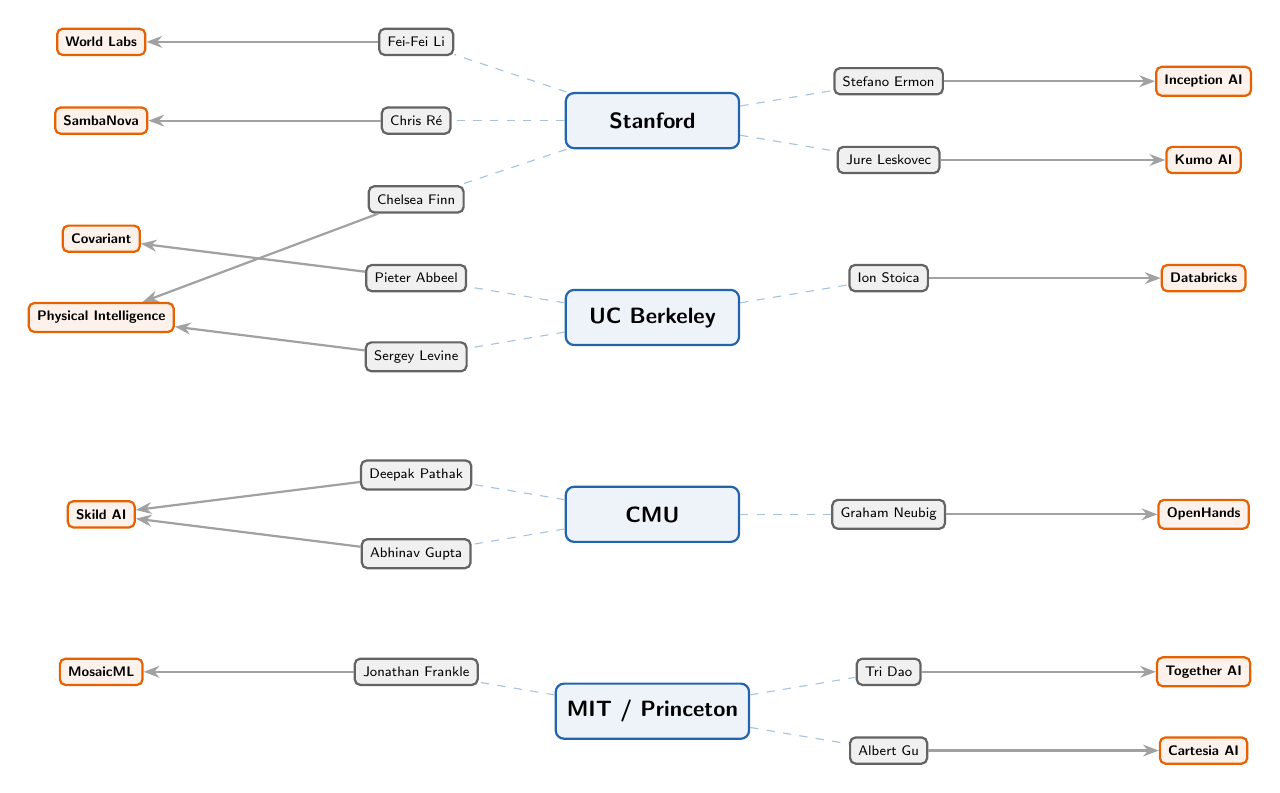
\begin{tikzpicture}[
  every node/.style={font=\sffamily\scriptsize},
  uni/.style={draw=figBlue, thick, fill=figBlue!8, rounded corners=3pt,
              inner sep=4pt, font=\sffamily\footnotesize\bfseries,
              minimum width=2.2cm, minimum height=0.7cm},
  prof/.style={draw=figGray, thick, fill=figLightGray, rounded corners=2pt,
               inner sep=3pt, font=\sffamily\tiny},
  co/.style={draw=figOrange, thick, fill=figOrange!8, rounded corners=2pt,
             inner sep=3pt, font=\sffamily\tiny\bfseries},
  arr/.style={-{Stealth[length=2mm]}, thick, figGray!60},
]

% Universities
\node[uni] (stan) at (0, 8) {Stanford};
\node[uni] (berk) at (0, 5.5) {UC Berkeley};
\node[uni] (cmu) at (0, 3) {CMU};
\node[uni] (mit) at (0, 0.5) {MIT / Princeton};

% Stanford professors
\node[prof] (ffl) at (-3, 9) {Fei-Fei Li};
\node[prof] (cre) at (-3, 8) {Chris R\'{e}};
\node[prof] (cf) at (-3, 7) {Chelsea Finn};
\node[prof] (se) at (3, 8.5) {Stefano Ermon};
\node[prof] (jl) at (3, 7.5) {Jure Leskovec};

% Berkeley professors
\node[prof] (pa) at (-3, 6) {Pieter Abbeel};
\node[prof] (sl) at (-3, 5) {Sergey Levine};
\node[prof] (is) at (3, 6) {Ion Stoica};

% CMU professors
\node[prof] (dp) at (-3, 3.5) {Deepak Pathak};
\node[prof] (ag) at (-3, 2.5) {Abhinav Gupta};
\node[prof] (gn) at (3, 3) {Graham Neubig};

% MIT/Princeton
\node[prof] (jf) at (-3, 1) {Jonathan Frankle};
\node[prof] (td) at (3, 1) {Tri Dao};
\node[prof] (agu) at (3, 0) {Albert Gu};

% Companies
\node[co] (wl) at (-7, 9) {World Labs};
\node[co] (sb) at (-7, 8) {SambaNova};
\node[co] (pi) at (-7, 5.5) {Physical Intelligence};
\node[co] (cov) at (-7, 6.5) {Covariant};
\node[co] (db) at (7, 6) {Databricks};
\node[co] (ski) at (-7, 3) {Skild AI};
\node[co] (oh) at (7, 3) {OpenHands};
\node[co] (mos) at (-7, 1) {MosaicML};
\node[co] (tog) at (7, 1) {Together AI};
\node[co] (car) at (7, 0) {Cartesia AI};
\node[co] (inc) at (7, 8.5) {Inception AI};
\node[co] (kum) at (7, 7.5) {Kumo AI};

% Arrows: prof -> university (abbreviated via positioning)
% Arrows: prof -> company
\draw[arr] (ffl) -- (wl);
\draw[arr] (cre) -- (sb);
\draw[arr] (cf) -- (pi);
\draw[arr] (sl) -- (pi);
\draw[arr] (pa) -- (cov);
\draw[arr] (is) -- (db);
\draw[arr] (dp) -- (ski);
\draw[arr] (ag) -- (ski);
\draw[arr] (gn) -- (oh);
\draw[arr] (jf) -- (mos);
\draw[arr] (td) -- (tog);
\draw[arr] (agu) -- (car);
\draw[arr] (se) -- (inc);
\draw[arr] (jl) -- (kum);

% University connections (dashed)
\draw[dashed, figBlue!40] (stan) -- (ffl);
\draw[dashed, figBlue!40] (stan) -- (cre);
\draw[dashed, figBlue!40] (stan) -- (cf);
\draw[dashed, figBlue!40] (stan) -- (se);
\draw[dashed, figBlue!40] (stan) -- (jl);
\draw[dashed, figBlue!40] (berk) -- (pa);
\draw[dashed, figBlue!40] (berk) -- (sl);
\draw[dashed, figBlue!40] (berk) -- (is);
\draw[dashed, figBlue!40] (cmu) -- (dp);
\draw[dashed, figBlue!40] (cmu) -- (ag);
\draw[dashed, figBlue!40] (cmu) -- (gn);
\draw[dashed, figBlue!40] (mit) -- (jf);
\draw[dashed, figBlue!40] (mit) -- (td);
\draw[dashed, figBlue!40] (mit) -- (agu);

\end{tikzpicture}
\caption{教授-创业管道：顶级大学的AI教授与他们创办的公司。
实线箭头表示创始人/联合创始人关系，
虚线表示所属大学。}
\label{fig:prof-startup}
\end{figure}

本章中呈现的研究者有一些值得注意的共同模式：

\begin{keybox}[五个关键观察]
\begin{enumerate}[noitemsep]
  \item \textbf{双重身份成为常态}：
        几乎所有顶级AI教授都同时在工业界担任顾问、
        研究VP或联合创始人。
        纯粹的``象牙塔''学术生涯在AI领域已经极为罕见。
  \item \textbf{开源是加速器}：
        FlashAttention、vLLM、OpenHands等项目
        都是先在学术界开源获得验证，
        再转化为商业产品。
        开源不仅是理想主义，更是高效的市场验证策略。
  \item \textbf{学生网络即竞争壁垒}：
        Pieter Abbeel、Jitendra Malik、Yoshua Bengio等
        ``学术教父''的真正资产是他们培养的学生网络。
        这些学生在OpenAI、Anthropic、Google DeepMind
        和数十家创业公司中担任关键角色。
  \item \textbf{评估是权力}：
        制定评估标准（HELM、SWE-bench、MMLU）
        的学术团队对整个行业有巨大的隐性影响力——
        他们定义了``什么算好''，
        从而塑造了所有实验室的研发方向。
  \item \textbf{理论最终会变现}：
        Sanjeev Arora的理论学生Tengyu Ma成了Stanford教授，
        Chris R\'{e}的systems思维孵化了SambaNova，
        Elad Hazan的优化理论催生了Google AI Princeton——
        基础理论研究的商业价值通常滞后5--10年，
        但一旦时机成熟，回报是指数级的。
\end{enumerate}
\end{keybox}

% ----- Summary Table -----
\begin{table}[htbp]
\centering
\caption{本章主要学术研究者总览（按机构分组）}
\label{tab:academics-summary}
\footnotesize
\begin{tabularx}{\textwidth}{l l X l}
\toprule
\textbf{姓名} & \textbf{机构} & \textbf{核心贡献} & \textbf{产业联系} \\
\midrule
% Stanford
Fei-Fei Li & Stanford & ImageNet、空间智能 & World Labs CEO \\
C.\ Manning & Stanford & GloVe、SAIL主任 & — \\
Percy Liang & Stanford & HELM、CRFM & Together AI \\
Chelsea Finn & Stanford & MAML、OpenVLA & Physical Intelligence \\
Chris R\'{e} & Stanford & Snorkel、Data-Centric AI & SambaNova, Together \\
Tri Dao & Princeton & FlashAttention、Mamba & Together AI CTO \\
Stefano Ermon & Stanford & DDIM、Score-based models & Inception AI CEO \\
Tengyu Ma & Stanford & 深度学习理论 & — \\
T.\ Hashimoto & Stanford & 数据高效LM & — \\
Jure Leskovec & Stanford & GraphSAGE & Kumo AI \\
Dorsa Sadigh & Stanford & 人机交互机器人学习 & — \\
\midrule
% Berkeley
Pieter Abbeel & Berkeley & 深度RL、TRPO、SAC & Amazon, Covariant \\
Stuart Russell & Berkeley & AI安全、CHAI & — \\
Sergey Levine & Berkeley & $\pi$0机器人基础模型 & Physical Intelligence \\
Ion Stoica & Berkeley & Spark、Ray & Databricks, Anyscale \\
Dawn Song & Berkeley & AI安全+去中心化 & Oasis Labs \\
Trevor Darrell & Berkeley & 深度视觉 & — \\
Jitendra Malik & Berkeley & 计算机视觉 & — \\
L.\ Zheng, W.\ Kwon & Berkeley & vLLM/PagedAttention & Inferact \\
\midrule
% CMU
R.\ Salakhutdinov & CMU & 深度学习+概率模型 & Meta VP \\
Graham Neubig & CMU & 代码生成、NLP & All Hands AI \\
Deepak Pathak & CMU & 机器人基础模型 & Skild AI CEO \\
Abhinav Gupta & CMU & 视觉学习+具身智能 & Skild AI 总裁 \\
\midrule
% MIT
Regina Barzilay & MIT & AI for Cancer & Jameel Clinic \\
Daniela Rus & MIT & CSAIL主任、机器人 & Venti, Themis AI \\
J.\ Frankle & MIT(PhD) & 彩票假说 & Databricks CAS \\
\midrule
% Princeton
Sanjeev Arora & Princeton & 深度学习理论 & PLI主任 \\
Danqi Chen & Princeton & Open-domain QA & — \\
K.\ Narasimhan & Princeton & SWE-bench & — \\
Elad Hazan & Princeton & 在线学习/优化 & Google AI Princeton \\
\midrule
% UW / AI2
Yejin Choi & UW→Stanford & 常识AI & NVIDIA, AI2 \\
H.\ Hajishirzi & UW & OLMo、T\"{u}lu & AI2 \\
Luke Zettlemoyer & UW & NLP预训练 & Meta FAIR \\
Ali Farhadi & UW & 计算机视觉 & AI2 CEO(2023--26) \\
\midrule
% Canada
Roger Grosse & UofT & 训练数据归因 & Anthropic \\
Jimmy Ba & UofT & Adam、LayerNorm & xAI(2023--26) \\
Aaron Courville & Mila & DL教科书、生成模型 & IVADO SD \\
David Duvenaud & UofT & Neural ODE & Anthropic(2023--24) \\
\midrule
% Other
Andrew Ng & Stanford & DL教育民主化 & AI Fund, Coursera \\
Jason Wei & — & CoT、Emergence & Meta SIL \\
Albert Gu & CMU & S4、Mamba & Cartesia AI \\
Stella Biderman & — & The Pile、GPT-NeoX & EleutherAI \\
Max Welling & Amsterdam & VAE & CuspAI \\
Yarin Gal & Oxford & 不确定性量化 & — \\
Been Kim & DeepMind & TCAV、可解释性 & Google DeepMind \\
Shakir Mohamed & DeepMind & AI for Social Good & Google DeepMind \\
Kyunghyun Cho & NYU & GRU、注意力机制 & — \\
\bottomrule
\end{tabularx}
\end{table}

\bigskip

学术界在AI领域的角色正在经历根本性的重塑。
传统的``大学研究→论文发表→毕业生进入工业界''
的线性路径已经被一个更加复杂、更加动态的网络所取代：
教授同时是创始人，博士生同时是CTO，
学术论文同时是产品路线图，
开源项目同时是商业原型。

这种模式的好处是显而易见的：
知识转化的速度大幅提升，
社会能够更快地从基础研究中获益。
但风险同样存在：
当评估标准的制定者同时是被评估公司的利益相关者，
当公开发表的研究背后有未披露的商业利益，
学术界作为``独立裁判''的角色就会受到侵蚀。

这是一个值得整个AI社区认真思考的治理挑战——
而解决方案，很可能也将来自学术界本身。

\chapter{声音、愿景与新星——AI 的良知、喉舌与未来力量}
\label{ch:policy-rising}
%% ============================================================
%% Chapter 14 — AI Policy, Ethics, Media Figures & Rising Stars
%% ============================================================

当技术以指数级速度演进时，
围绕技术的\textbf{叙事}——谁来讲述、谁来质疑、谁来规范——
往往决定了技术最终服务于谁。
2023--2026 年的 AI 浪潮中，
一群政策制定者、伦理学者、科普传播者、开源英雄和年轻创业者
从不同角度塑造了这场革命的面貌。
他们不一定训练模型，但他们定义了模型被训练的\emph{边界}、
被使用的\emph{方式}和被理解的\emph{语境}。

本章覆盖五个互相交织的群体：
制定规则的\textbf{政策人物}、
发出警告的\textbf{伦理学者}、
连接公众与前沿的\textbf{媒体与公共知识分子}、
构建共享基础设施的\textbf{开源社区英雄}、
以及正在重新定义可能性边界的\textbf{35 岁以下新星}。

%% ============================================================
\section{AI 政策：监管者追赶技术}
\label{sec:policy}
%% ============================================================

2023 年是 AI 监管的「觉醒之年」。
在 ChatGPT 发布不到一年后，
全球主要经济体几乎同时启动了各自的 AI 治理框架。
这种速度在技术监管史上前所未有——
相比之下，互联网经历了近 20 年才迎来第一部全面的数据隐私法规（GDPR，2018）。

\subsection{美国：行政令与芯片管制的双重策略}

美国的 AI 治理采取了一种独特的「双轨制」：
行政令（Executive Order）处理国内安全与创新，
出口管制（Export Controls）处理地缘政治竞争。

\textbf{Kamala Harris}（1964--）作为副总统，
成为 Biden 政府 AI 政策的核心推动者和公众面孔。
2023 年 10 月 30 日，Biden 签署了美国历史上第一份
AI 行政令（Executive Order on the Safe, Secure, and Trustworthy
Development and Use of Artificial Intelligence），
Harris 在签字仪式上鼓掌的画面成为标志性时刻。
该行政令要求：
开发双用途基础模型（dual-use foundation models）的公司
在发布前必须向联邦政府报告安全测试结果；
商务部制定 AI 红队测试（red-teaming）标准；
联邦机构任命首席 AI 官（Chief AI Officers）。
Harris 随后亲赴 2023 年 11 月的 Bletchley Park AI 安全峰会，
代表美国发布了关于 AI 安全的新倡议，
包括成立美国 AI 安全研究所（US AI Safety Institute，隶属 NIST）。
2024 年 3 月，她宣布了 OMB 的首份联邦 AI 使用政策，
标志着从「自愿承诺」向「制度约束」的转变。

\begin{whybox}[为什么行政令而非立法？]
美国国会在 AI 立法上进展缓慢——
截至 2026 年初，仍未通过任何联邦级别的综合性 AI 法案。
行政令虽然法律效力有限（可被下一任总统撤销），
但它能在数周内生效，不需要经历旷日持久的两党博弈。
Biden 团队选择行政令，本质上是一种
``先建立框架、再推动立法'' 的策略。
事实上，Trump 在 2025 年 1 月就任后迅速撤销了该行政令，
证明了这种路径的脆弱性。
\end{whybox}

\textbf{Bruce Reed}（1960--）是这些政策背后的关键操盘手。
作为白宫副幕僚长（Deputy Chief of Staff），
Reed 负责协调跨部门的 AI 政策制定，
被《Politico》称为 ``Biden AI 政策的大脑''。
他的团队在不到 90 天内完成了行政令的起草——
这在白宫的政策制定流程中堪称闪电速度。
Reed 此前在 Clinton 政府时期就负责过互联网政策，
他将那个时代的经验——``不要过早扼杀创新，但要建立安全护栏''——
带入了 AI 治理。

\textbf{Gina Raimondo}（1971--）作为商务部长，
掌控着美国 AI 地缘战略中最锋利的武器：芯片出口管制。
2022 年 10 月，商务部产业与安全局（BIS）发布了对华芯片出口限制，
禁止向中国出口先进 AI 芯片（如 NVIDIA A100/H100）
和先进制程半导体设备。
Raimondo 在一次 CBS 采访中坦言：
``今天的国家安全不只是坦克和导弹，而是技术。
是半导体，是 AI，是无人机。''
她主导了三轮逐步升级的出口管制：
2022 年 10 月（初始限制）、
2023 年 10 月（堵住 NVIDIA 通过降规格芯片绕过管制的漏洞）、
2024 年 12 月（扩展至 24 类芯片制造设备和 140 个实体清单新增条目）。
2025 年 1 月 13 日，在 Biden 政府的最后几天，
她发布了最全面的 AI 出口管制框架，
按国家分三级（盟友/中立/受限）分配 AI 芯片配额。
Raimondo 的策略核心是：
\emph{不追求彻底脱钩（decoupling），
而是精准管控关键瓶颈技术}。

\begin{corebox}[芯片管制的意外后果]
Raimondo 的出口管制在遏制中国获取最先进 AI 芯片方面取得了部分成功，
但也产生了深远的意外后果：
它加速了中国 AI 芯片自主化的进程
（华为昇腾 910B/C 的快速迭代即是直接回应），
催生了复杂的灰色市场走私网络，
并促使 DeepSeek 等中国实验室在软件层面进行极致优化——
DeepSeek V3 在受限的 H800 集群上实现了与 H100 集群可比的训练效率，
某种程度上证明了出口管制的``水床效应''：
按下一处，另一处鼓起。
\end{corebox}

\subsection{英国：Bletchley Park 与 AI 安全研究所}

英国选择了一条与美国和欧盟不同的道路：
不急于立法，而是聚焦于\textbf{技术安全评估}。
这一策略的执行者是
\textbf{Ian Hogarth}（1983--），
一位天使投资人和科技企业家。

Hogarth 在 2023 年 6 月发表了一篇广受关注的
\emph{Financial Times} 文章 ``We Must Slow Down the Race to God-Like AI''，
随后被 Rishi Sunak 首相任命为英国前沿 AI 任务组
（Frontier AI Taskforce）的负责人。
2023 年 11 月 1--2 日，在具有深刻象征意义的 Bletchley Park
（二战密码破解中心、Alan Turing 的工作地）
举行了全球首届 AI 安全峰会（AI Safety Summit）。
28 国代表（包括中国）签署了《Bletchley 宣言》，
承认了 frontier AI 的潜在风险，
并同意在安全测试方面开展国际合作。

峰会的核心成果是英国 AI 安全研究所
（UK AI Safety Institute, AISI）的正式成立，
Hogarth 出任首任所长。
AISI 的任务是：在 frontier model 发布前后对其进行安全评估，
检测有害能力（如生化武器知识生成、网络攻击辅助）。
这种``政府级红队测试''的模式启发了美国（NIST AI Safety Institute）、
日本和加拿大建立类似机构。

\begin{keybox}[Bletchley Park 的符号意义]
选择 Bletchley Park 作为峰会地点并非巧合：
1940 年代，Turing 和团队在这里破解了 Enigma 密码，
改变了二战进程。80 年后，
各国领导人在同一地点讨论如何应对 Turing 的智力遗产
所带来的最深远挑战。
这种历史回响赋予了峰会超越外交辞令的叙事力量。
\end{keybox}

\subsection{欧盟：AI Act——全球首部综合性 AI 法案}

如果说美国靠行政令、英国靠安全评估，
欧盟则选择了它最擅长的工具：\textbf{立法}。

EU AI Act 的立法历程始于 2021 年 4 月的欧盟委员会提案，
历经近三年的谈判，于 2024 年 3 月 13 日
以 523 票赞成、46 票反对的压倒性多数在欧洲议会通过。
这是全球第一部全面的、具有法律约束力的 AI 监管框架。

三位关键推动者值得记录：

\textbf{Thierry Breton}（1955--），
法国人，时任欧盟内部市场专员（Commissioner for Internal Market）。
Breton 是 AI Act 在欧盟委员会层面的首席推动者。
他在 AI Act 通过后高调宣布：
``欧洲现在是 AI 的全球标准制定者。
我们监管尽可能少——但必要时绝不手软。''
Breton 此前是 Atos（欧洲最大 IT 服务公司之一）的 CEO，
他将企业家的务实与监管者的决心结合在一起。
他坚持 AI Act 必须覆盖通用目的 AI 模型（GPAI），
这一条款在最终版本中成为最具争议也最具影响力的部分。

\textbf{Dragoș Tudorache}（1972--），
罗马尼亚人，欧洲议会议员，AI Act 在议会的两位联合报告人之一。
Tudorache 此前是罗马尼亚内政部长，
他回忆说自己对 AI 的兴趣始于 2015 年阅读 Nick Bostrom 的
\emph{Superintelligence} 一书。
他与意大利议员 \textbf{Brando Benifei} 搭档，
花了两年时间在欧洲议会中推动 AI Act 的通过。
Tudorache 在接受 \emph{MIT Technology Review} 采访时表示：
``没有人以前做过这样的事。
这不是从架子上拿一份旧模板就能完成的。''

AI Act 的核心是一个\textbf{风险分级框架}：
\begin{itemize}[noitemsep]
  \item \textbf{不可接受风险}（Unacceptable Risk）：
        社会信用评分、实时远程生物识别（执法例外除外）——直接禁止。
  \item \textbf{高风险}（High Risk）：
        关键基础设施、教育、就业中的 AI 系统——需通过合规评估。
  \item \textbf{有限风险}：
        聊天机器人、深度伪造——需透明度义务（标注 AI 生成内容）。
  \item \textbf{最低风险}：
        垃圾邮件过滤器等——不受额外监管。
\end{itemize}

对通用目的 AI 模型（GPAI）的特别条款要求：
所有 GPAI 提供者必须提供模型卡（model cards）和技术文档；
被认定为具有``系统性风险''的模型（训练算力超过 $10^{25}$ FLOPs）
还必须进行对抗性安全测试并向欧洲 AI 办公室报告严重事件。

\subsection{中国：渐进式、分领域的 AI 治理}

中国的 AI 治理路径与西方截然不同。
中国没有选择``一步到位的综合立法''，
而是采取了\textbf{渐进式、分领域的监管策略}——
先针对具体场景出台规定，再逐步构建统一框架。

三部关键法规构成了中国 AI 治理的基础框架：
\begin{itemize}[noitemsep]
  \item \textbf{《互联网信息服务算法推荐管理规定》}
        （2022 年 3 月生效）：
        规范推荐算法，要求算法透明度和用户选择权。
  \item \textbf{《互联网信息服务深度合成管理规定》}
        （2023 年 1 月生效）：
        针对深度伪造（deepfake）技术，
        要求内容标识和备案管理。
  \item \textbf{《生成式人工智能服务管理暂行办法》}
        （2023 年 8 月生效）：
        这是全球首个专门针对生成式 AI 的监管法规，
        要求备案审批、内容安全和数据合规。
\end{itemize}

2025 年 10 月，修订后的《网络安全法》
新增了专门的``人工智能合规''条款，
标志着 AI 治理正式被纳入中国网络安全的顶层法律架构。
同时，2025 年 8 月国务院发布的
《关于深入实施``人工智能+''行动的意见》
则代表了另一个方向：
以政策激励推动 AI 与实体经济的深度融合，
设定了到 2027 年 AI 应用普及率超 70\%、
2030 年超 90\% 的宏大目标。

\begin{whybox}[中国为什么没有出台综合性 AI 法？]
2025 年，中国曾将综合性 AI 立法列入计划议程，
但随后将其移出。
分析认为，这并非``放弃监管''，
而是务实地认识到：
在 AI 技术快速迭代的阶段，
过早的综合立法可能抑制创新。
相比之下，``先试点、再标准、再立法''的路径
允许监管者通过观察 DeepSeek、Kimi 等国产模型的实际部署效果
来校准监管力度。
这种方法更灵活，但也导致了
企业面临多套重叠规则的``法规碎片化''挑战。
\end{whybox}

\subsection{Yoshua Bengio：从学术殿堂到政策前线}

\textbf{Yoshua Bengio}（1964--）
是深度学习三巨头之一（2018 年图灵奖共同获得者），
但在 2023--2026 年间，他的角色发生了深刻转变：
从纯粹的学术研究者变成了全球 AI 安全政策的首席科学顾问。

2023 年 7 月，Bengio 在美国参议院隐私与技术小组委员会作证，
呼吁政府投资 AI 安全研究并建立监管框架。
2023 年 11 月的 Bletchley Park 峰会后，
他被委托领导《国际 AI 安全科学报告》
（International Scientific Report on the Safety of Advanced AI）——
一个受 IPCC（政府间气候变化专门委员会）启发的倡议，
由 30 多个国家的代表支持，
超过 100 位独立专家参与撰写。
临时报告于 2024 年 5 月的首尔 AI 峰会发布，
完整版于 2026 年 2 月的巴黎 AI 行动峰会发布。

Bengio 的转变在 AI 社区引发了争议。
一些同行（尤其是 Yann LeCun）批评他的安全立场过于悲观，
认为当前的 AI 系统距离 AGI 还很遥远。
Bengio 的回应是：
``我宁愿因为过早发出警告而被嘲笑，
也不愿因为沉默而在灾难发生后被追责。''

%% ============================================================
\section{AI 伦理：技术的良心}
\label{sec:ethics}
%% ============================================================

如果说政策制定者从\emph{外部}为 AI 设定边界，
伦理学者则从\emph{内部}审视 AI 的价值观、偏见和权力结构。
2020--2026 年间，一系列标志性事件——
Google 伦理 AI 团队的解散、``随机鹦鹉''论文的发表、
面部识别偏见的曝光——
将 AI 伦理从学术角落推到了公众聚光灯下。

\subsection{Google 伦理 AI 风暴：Timnit Gebru 与 Margaret Mitchell}

2020 年 12 月，Google 伦理 AI 团队联合负责人
\textbf{Timnit Gebru}（1982/1983--）的离职
成为 AI 伦理领域的分水岭事件。

Gebru 是一位厄立特里亚裔埃塞俄比亚出生的计算机科学家，
在加入 Google 前已是 AI 公平性研究的先驱——
她共同创立了 Black in AI，
一个推动更多黑人参与 AI 研发的倡导组织。
在 Google，她与 Margaret Mitchell 共同领导伦理 AI 团队，
建立了一支包含大量少数族裔成员的研究小组。

导火索是一篇论文。
Gebru 与 Emily Bender、Mitchell 等人合著了
``On the Dangers of Stochastic Parrots:
Can Language Models Be Too Big?''，
系统性地分析了大型语言模型的风险：
环境成本（训练的碳排放）、
训练数据中嵌入的社会偏见、
以及模型``看起来流利但不理解''的根本局限。
据 Gebru 所述，Google 管理层要求她撤回论文或移除所有 Google 员工的署名。
当她要求知晓审稿人身份和具体反馈时，
被告知``已经接受了辞职''——Gebru 否认自己曾辞职，
坚称这是被解雇。

两个月后，2021 年 2 月，
\textbf{Margaret Mitchell}（也被解雇。
Google 声称她违反了公司行为准则，
将文件转移到公司外部。
Mitchell——一位在自然语言生成、
视觉描述和模型偏见评估方面有深厚积累的研究者——
否认了不当行为。

\begin{corebox}[``Stochastic Parrots'' 论文的深远影响]
``随机鹦鹉''论文最初因 Google 内部的审查争议而广为人知，
但它的学术价值远超其引发的公关危机。
论文提出的核心论点——
大型语言模型本质上是在``拼接''训练数据中的模式，
而非真正``理解''语言——
成为此后所有关于 LLM 能力边界讨论的起点。
该论文发表于 2021 年 ACM FAccT 会议。
值得注意的是，Mitchell 的署名被化名为
``Shmargaret Shmitchell''，
这个黑色幽默式的伪名本身就成了对学术审查的无声抗议。
有趣的是，2026 年 3 月，
Mitchell 本人撰文 ``No, `AI' is not a Stochastic Parrot''，
对该术语的\emph{过度简化使用}进行了反思——
她区分了论文的原始论点（警告过度依赖规模）
与某些人将其简化为``AI 不可能有任何能力''的误读。
\end{corebox}

Gebru 离开 Google 后创立了
\textbf{DAIR 研究所}（Distributed AI Research Institute），
一个独立于大型科技公司的 AI 研究机构，
致力于以社区为中心的 AI 研究。
Mitchell 则于 2021 年 10 月加入 Hugging Face，
担任首席伦理科学家（Chief Ethics Scientist），
在那里她将伦理原则嵌入开源 AI 平台的架构中——
这被 \emph{TIME} 杂志 2023 年 ``AI 百大影响力人物''
选中为标志性案例，
证明伦理不只是批评，也可以是\emph{建设}。

\subsection{Emily Bender：语言学家的警告}

\textbf{Emily Bender}（约 1973--）
是华盛顿大学的计算语言学教授，
``随机鹦鹉''论文的第一作者。
与许多 AI 研究者不同，
Bender 的学术根基在\emph{语言学}而非计算机科学。
这种独特的视角使她能够提出一个
许多 AI 从业者不愿面对的问题：
\emph{LLM 是在使用语言，还是在模拟使用语言的统计模式？}

Bender 是 AI 批评界最一致的声音之一。
在 2024 年 11 月 Harvey Mudd College 的演讲中，
她将 RAG（检索增强生成）比作``用好数据做的纸浆模型——
材料更好了，但本质上还是纸浆''。
她的核心观点可以概括为三个层次：
\begin{enumerate}[noitemsep]
  \item LLM 的输出正确时，这在很大程度上是\emph{偶然}的；
  \item 流利性（fluency）不等于理解（comprehension）；
  \item 将 LLM 的输出当作``知识''是一种危险的范畴错误。
\end{enumerate}

\subsection{Joy Buolamwini：揭示算法歧视的``诗人战士''}

\textbf{Joy Buolamwini}（约 1990--）的故事
始于一个简单而令人不安的发现：
作为 MIT Media Lab 的研究生，
她发现面部识别软件无法检测到她的面孔——
除非她戴上一张白色面具。

这个个人经历推动她进行了系统性研究。
她的 \textbf{Gender Shades} 项目（2018）揭示了
IBM、Microsoft 和 Face++ 的商业面部识别系统中的严重偏见：
对深肤色女性的错误率高达 34.7\%，
而对浅肤色男性仅为 0.8\%。
这一 43 倍的差距——不是抽象的统计数字，
而是真实的人被错误识别、错误逮捕、错误排斥的风险。

Buolamwini 创立了\textbf{算法正义联盟}
（Algorithmic Justice League, AJL），
她将自己定位为``诗人战士''（poet of code），
因为她在技术抗议中融入了说唱和表演艺术。
AJL 的使命不仅是技术审计，
更是``建立受影响社区的声音和选择权''。

她的工作产生了直接的政策影响：
IBM 在 2020 年宣布退出通用面部识别市场，
明确引用了偏见问题；
多个美国城市（包括旧金山、波士顿）
通过了限制政府使用面部识别的法规。

\subsection{Meredith Whittaker：从 Google 罢工到 Signal 总裁}

\textbf{Meredith Whittaker}（约 1977--）
的职业轨迹本身就是一部 AI 伦理运动的缩影。

在 Google 工作 13 年期间，
她创立了 Google 的 Open Research 项目，
并共同创立了\textbf{AI Now 研究所}
（AI Now Institute，纽约大学）——
全球最早的跨学科 AI 社会影响研究机构之一（2017）。
2018 年 11 月，她参与组织了
Google 历史上最大规模的员工罢工（Google Walkout），
抗议公司对性骚扰投诉的处理方式以及与军方的 AI 合作（Project Maven）。

罢工后，Whittaker 表示被告知如果要留在 Google，
必须放弃 AI 伦理工作和在 AI Now 的角色。
她选择在 2019 年离开。
此后她担任 FTC（联邦贸易委员会）主席 Lina Khan 的顾问，
并于 2022 年 9 月被任命为\textbf{Signal}
（加密通信应用）的首任总裁。

Whittaker 在 Signal 的角色将她的 AI 批评
与一个具体的替代愿景结合在一起：
如果大型科技公司的商业模式本质上依赖监控，
那么 Signal 所代表的\emph{加密、非营利、开源}模式
就是一种结构性的反命题。

\subsection{Kate Crawford：AI 的``政治经济学''}

\textbf{Kate Crawford}（约 1976--）是 AI Now 研究所的联合创始人，
USC Annenberg 的研究教授。
她的 2021 年著作 \emph{Atlas of AI: Power, Politics,
and the Planetary Costs of Artificial Intelligence}
开创性地将 AI 分析的视角从``算法''扩展到``供应链''：
从内华达州的锂矿到亚马逊仓库的工人，
从 ImageNet 数据集中的标注偏见到军事监控的应用。

Crawford 的核心论点是：
AI 既不是``人工的''也不是真正``智能的''——
它是一个建立在\emph{人类劳动、自然资源提取和权力不对称}
之上的社会技术系统。
\emph{Atlas of AI} 被 \emph{New Yorker} 称为
``对机器学习训练数据的迷人历史''，
被 \emph{Science} 称为``及时而紧迫的贡献''。

\subsection{Safiya Noble：搜索引擎的种族政治}

\textbf{Safiya Umoja Noble}（约 1975--）
是 UCLA 信息学教授，
她的 2018 年著作 \emph{Algorithms of Oppression:
How Search Engines Reinforce Racism}
通过一个简单实验揭示了深层问题：
在 Google 中搜索 ``Black girls'' 得到的结果
与搜索 ``white girls'' 截然不同——
前者充斥着色情化内容，后者则相对中性。

Noble 的工作将``算法偏见''的讨论从面部识别
扩展到了\emph{信息检索}——
一个看似中立但实际上深度嵌入了社会权力结构的技术领域。
她指出，搜索引擎的排名算法不是``客观的''，
而是反映了广告商的商业利益和社会的既有偏见。

\subsection{Gary Marcus：AI 最响亮的怀疑者}

\textbf{Gary Marcus}（1970--）的角色很独特：
他既不是伦理学者也不是政策制定者，
而是一个在 AI 能力问题上最持久、最高调的\textbf{技术怀疑者}。

Marcus 是 NYU 心理学与神经科学荣休教授，
认知科学家，著有多本 AI 通俗读物。
2016 年，他创立了 Geometric Intelligence
（一家将认知科学与机器学习结合的 AI 初创公司），
后被 Uber 收购。
他还在美国参议院 AI 听证会上作证。

2022 年，Marcus 发表了引发广泛争议的文章
``Deep Learning is Hitting a Wall''，
预测深度学习在可靠性和推理能力上的根本瓶颈。
AI 圈对他的态度高度两极化——
支持者称他为``AI 的良心''，
批评者称他为``永远唱衰的人''（Elon Musk 曾转发讽刺他的 meme）。
然而，Marcus 2024 年初在 \emph{IEEE Spectrum} 的访谈中指出，
他关于可靠性问题的许多预测已经被验证：
幻觉（hallucination）仍然是 LLM 最难解决的问题之一。

Marcus 自己的总结颇为精辟：
``讽刺是针对我的；失败是深度学习之主的。''

\subsection{Melanie Mitchell：复杂性视角下的 AI}

\textbf{Melanie Mitchell}（约 1969--）
是圣塔菲研究所（Santa Fe Institute）教授，
她的独特贡献在于从\textbf{复杂系统科学}的视角分析 AI。
她的著作 \emph{Complexity: A Guided Tour}（2010，获 Phi Beta Kappa 奖）
和 \emph{Artificial Intelligence: A Guide for Thinking Humans}（2019）
为非技术读者提供了理解 AI 的深度框架。

Mitchell 的研究聚焦于``概念抽象和类比推理''——
她认为这些是人类智能的核心，
也是当前 AI 系统最薄弱的环节。
她既不属于``AI 将毁灭人类''的末日论阵营，
也不属于``深度学习能解决一切''的乐观派，
而是坚持一种基于证据的、精细的中间立场。

%% ============================================================
\section{AI 媒体与公共知识分子}
\label{sec:media}
%% ============================================================

AI 革命的独特之处在于它的\textbf{极度公开性}。
与过去的技术革命不同（半导体革命发生在洁净室里，
互联网革命发生在大学实验室里），
AI 革命很大程度上发生在 YouTube、Twitter/X、
Substack 和播客上。
一批``翻译者''——将前沿论文转化为公众理解的人——
成为了 AI 时代不可或缺的角色。

\subsection{Lex Fridman：AI 时代的 Charlie Rose}

\textbf{Lex Fridman}（1983--），
出生于苏联塔吉克斯坦的美裔计算机科学家和播客主持人。
他在 Drexel University 获得学士、硕士和博士学位，
此后在 MIT 人工智能实验室和 AgeLab 担任研究员。
2018 年起，他开始主持 \emph{Lex Fridman Podcast}，
至今已制作超过 460 期，
嘉宾涵盖 Elon Musk、Sam Altman、Mark Zuckerberg、
Jensen Huang、Yann LeCun、Jeff Bezos 乃至
印度总理 Narendra Modi。

Fridman 的访谈风格——超长形式（通常 2--4 小时）、
深度技术问题与哲学思考交织、
极其温和的追问方式——使他成为 AI 领域最有影响力的媒体人之一。
批评者认为他对嘉宾过于客气，缺乏批判性追问；
支持者则认为这种方式让嘉宾放松后更可能吐露真实想法。
无论如何，``上 Lex 的播客''已成为 AI 领袖
向科技社区传达信息的标准渠道。

Fridman 2019 年因 Elon Musk 赞扬他一篇关于 Tesla Autopilot
驾驶员注意力的研究而迅速走红——
尽管该研究未经同行评审并受到 AI 专家批评。
自 2022 年起他切换为 MIT 无薪职位，
全职投入播客和内容创作。
截至 2026 年，他的 YouTube 频道拥有数百万订阅者。

\subsection{Andrej Karpathy：从研究到教育的全栈 AI 人}

\textbf{Andrej Karpathy}（1986--）
可能是 AI 领域最成功的``知识翻译者''。
他是 OpenAI 的创始团队成员（2015），
后任 Tesla 自动驾驶（Autopilot / FSD）负责人（2017--2022），
再回到 OpenAI（2023），最终于 2024 年离开创立
\textbf{Eureka Labs}——一个``AI 原生''教育平台。

但 Karpathy 最深远的影响力来自他的\emph{教育内容}。
他在 Stanford 开设的 CS231n（卷积神经网络与视觉识别）
是深度学习教育史上最有影响力的课程之一。
他的 YouTube 频道以极其清晰的风格
从零讲解神经网络、GPT、Tokenizer 等核心概念——
他 2023 年的视频 ``Let's Build GPT from Scratch''
在数周内获得数百万播放量，
使数以万计的工程师第一次真正理解了 Transformer 的工作原理。

Karpathy 的独特之处在于他的\emph{全栈经历}：
他既做过前沿研究（ImageNet 上的 CNN），
也管理过大规模工程团队（Tesla 数百人的 Autopilot 团队），
还能将这些经验转化为任何人都能跟随的教程。
Eureka Labs 是他将这种能力制度化的尝试——
用 AI 辅助教学，让``世界上最好的老师''能够扩展到百万学生。

\subsection{Grant Sanderson (3Blue1Brown)：数学可视化的魔术师}

\textbf{Grant Sanderson}（约 1988--）
创建的 YouTube 频道 3Blue1Brown
用精美的数学动画解释了从线性代数到神经网络的核心概念。
他的``But What is a Neural Network?'' 系列（2017 年首发，2026 年更新）
可能是互联网上对神经网络最直观的入门解释。

Sanderson 的贡献看似``只是科普''，
但其实际影响不可低估：
对于一代在 AI 浪潮中成长的学生来说，
3Blue1Brown 的动画是他们理解高维空间、
反向传播和注意力机制的第一扇窗口。
2026 年 2 月，他受邀在 UC Santa Cruz 演讲，
主题是``高维球体的美与实用''——
而听众中的许多人正是因为他的视频才对数学产生了兴趣。

\subsection{Lilian Weng：从博客到 OpenAI 副总裁}

\textbf{Lilian Weng}是一个罕见的案例：
她的\emph{个人博客}可能比许多研究论文
产生了更大的教育影响力。

Weng 出生于中国，在北京航空航天大学获学士学位，
后在卡内基梅隆大学获计算机科学博士学位。
2018 年加入 OpenAI，
她从 2017 年起维护的博客 \textbf{Lil'Log}
（lilianweng.github.io）
以极其清晰、系统的长文
覆盖了从强化学习到扩散模型到
test-time compute 的几乎所有 LLM 核心主题。
每篇文章都像一部迷你教科书，
包含大量公式推导、代码片段和精心绘制的图表。

到 2025 年中，
Weng 已晋升为 OpenAI 研究与安全副总裁
（VP of Research and Safety），
接替此前一系列离职高管的空缺。
她的轨迹体现了一种独特的职业路径：
\emph{通过公开的知识贡献建立声望，
再将这种声望转化为组织内部的领导力。}

\subsection{Jeremy Howard 与 Rachel Thomas：AI 民主化的先驱}

\textbf{Jeremy Howard}（1973--）和
\textbf{Rachel Thomas}（约 1980--）
在 2016 年共同创立了 \textbf{fast.ai}，
这是 AI 教育史上最重要的项目之一。

Howard 的背景非同寻常：
他曾是 Kaggle 平台的总裁和首席科学家，
两次获得国际机器学习竞赛排名第一；
他创立了 Enlitic（第一家将深度学习应用于医疗的公司），
被 \emph{MIT Technology Review} 连续两年评为
全球 50 大最聪明公司。

fast.ai 的哲学与当时主流的``先学三年数学再碰代码''的
深度学习教育方式截然相反。
Howard 和 Thomas 借鉴了教育家 Paul Lockhart 的理念——
不要让学生在接触真正的创造之前
花费数年在干燥的理论基础上——
设计了``自上而下''的课程：
第一节课就训练一个图像分类器，
理论在实践中逐步引入。

Thomas 不仅是 fast.ai 的联合创始人，
还是 AI 伦理教育的开拓者——
她是 USF 数据伦理课程的首位讲师，
将 AI 公平性和社会影响整合进了技术教育。
她后来担任了 fast.ai 的首席执行官。

\subsection{其他重要的 AI 传播者}

\textbf{Chip Huyen}（约 1992--）是一位越南裔的 AI 系统工程师和作家。
她在越南的稻田村庄长大，
后在 Stanford 教授``机器学习系统设计''课程。
她的著作 \emph{Designing Machine Learning Systems}（2022）
成为 Amazon AI 类目的 \#1 畅销书，翻译成 10+ 种语言；
2025 年的 \emph{AI Engineering} 一书
自上市以来一直是 O'Reilly 平台上阅读量最高的书籍。
她此前在 NVIDIA（NeMo 核心开发者）、Snorkel AI 和 Netflix 工作，
还创立并出售了一家 AI 基础设施创业公司。

\textbf{Sebastian Raschka}（约 1989--）是威斯康星大学麦迪逊分校的
统计学助理教授，后加入 Lightning AI 担任首席 AI 教育官。
他的著作 \emph{Machine Learning with PyTorch and Scikit-Learn}
以及 \emph{Build a Large Language Model (From Scratch)}
以``代码优先''的风格解释了从经典 ML 到 LLM 的全栈知识。
他的博客和 Twitter 内容是 ML 社区中被引用最频繁的教育资源之一。

\textbf{李沐}（Mu Li）是前 Amazon Web Services 应用科学家，
他与 Aston Zhang 等人合著的
\emph{Dive into Deep Learning}（D2L，《动手学深度学习》）
是全球被 70 个国家 500+ 所大学采用的交互式深度学习教材。
他的中文 YouTube 频道``跟李沐学 AI''
为中文世界提供了高质量的 AI 教育内容。
D2L 的独特之处在于它是\emph{可执行的}——
每一章的代码都可以直接在 Jupyter Notebook 中运行。

\textbf{Yannic Kilcher} 是一位瑞士的 ML 研究者和 YouTube 创作者，
以逐页拆解最新 AI 论文而闻名。
他的视频覆盖了从 GPT-4 技术报告到 Mamba 论文的几乎所有重要工作，
风格直接、不加修饰，偶尔尖锐——
他是许多研究者了解新论文的第一站。

\subsection{AI 哲学家与未来学家}

\textbf{Ray Kurzweil}（1948--）
是 AI 未来学领域最具影响力（也最具争议性）的声音。
他的 2005 年著作 \emph{The Singularity Is Near}
预测``技术奇点''——人工智能超越人类智能的时刻——将在 2045 年到来。
自 2012 年起，他在 Google 担任工程总监，
致力于自然语言处理和语音识别。
2024 年，他出版了续作 \emph{The Singularity Is Nearer}，
声称 AI 的进展正在验证他二十年前的预测。
Kurzweil 的``加速回报定律''——
技术进步的速度本身在指数级加速——
对整整一代 AI 创业者产生了深刻影响，
尽管许多学术研究者认为他的预测过于乐观。

\textbf{Nick Bostrom}（1973--），
瑞典哲学家，牛津大学教授，
人类未来研究所（Future of Humanity Institute, FHI）创始主任。
他的 2014 年著作 \emph{Superintelligence: Paths, Dangers, Strategies}
是 AI 安全运动的奠基性文本之一——
从 Elon Musk 到 Bill Gates，
许多科技领袖都引用该书作为他们关注 AI 风险的原因。
Bostrom 将``超级智能''定义为
``在几乎所有认知领域大幅超越人类的智力''，
并分析了``控制问题''——
一旦超级智能出现，我们如何确保它的目标与人类一致？
FHI 于 2024 年关闭，
但 Bostrom 继续通过 Macrostrategy Research Initiative 从事 AGI 治理研究。
他 2024 年的新书 \emph{Deep Utopia} 探讨了
一个``所有问题都被 AI 解决''的世界中人类意义的问题。

\textbf{Max Tegmark}（1967--），
瑞典裔美国物理学家，MIT 教授。
他的 2017 年著作 \emph{Life 3.0: Being Human in the Age of
Artificial Intelligence} 将 AI 的讨论
放置在宇宙学的宏大框架中：
如果 Life 1.0 是生物演化（硬件和软件都由自然选择决定），
Life 2.0 是文化演化（软件可以学习，硬件仍由进化决定），
那么 Life 3.0 就是 AI 时代——
``硬件和软件都可以自我设计''。
Tegmark 共同创立了
Future of Life Institute（FLI），
该组织在 2023 年发起了要求暂停训练
比 GPT-4 更强大的 AI 模型 6 个月的公开信，
获得超过 33,000 个签名（包括 Elon Musk、Steve Wozniak、
Yoshua Bengio 等知名人物），
成为 AI 安全讨论中的标志性事件——
尽管实际上没有任何实验室真正暂停了训练。

\textbf{Yuval Noah Harari}（1976--），
以色列历史学家，
\emph{Sapiens} 和 \emph{Homo Deus} 的作者。
Harari 并非 AI 技术专家，
但他对 AI 对人类社会、劳动、意识和权力结构影响的分析
使他成为全球最受关注的 AI 评论者之一。
他在多次演讲中警告：
AI 不需要``有意识''就能颠覆人类社会——
它只需要比人类更擅长\emph{操纵叙事}。

\textbf{李开复}（Kai-Fu Lee，1961--）
在中美 AI 界都拥有独特的双重影响力。
他曾任 Apple 语音识别研究负责人、
Microsoft 全球副总裁、Google 中国区总裁，
后创立创新工场（Sinovation Ventures）。
他的 2018 年著作 \emph{AI Superpowers: China, Silicon Valley,
and the New World Order} 是向西方世界解释
中国 AI 生态系统的最有影响力的作品。
2023 年，他创立了 \textbf{01.AI}
并推出了 Yi 系列开源大模型，
使他从 AI 评论家转变为 AI 实践者——
少有人能同时在\emph{写关于} AI 和\emph{做} AI 两个维度上
保持顶级影响力。

%% ============================================================
\section{下一代：35 岁以下的新星}
\label{sec:rising}
%% ============================================================

AI 领域最令人振奋的特征之一是它的\textbf{年轻化}。
在大多数技术领域，
重大影响通常需要数十年的积累；
但在 AI 的当前浪潮中，
一群 25--35 岁的年轻人正在以创始人、
关键论文作者或核心工程师的身份
重新定义可能性的边界。

\subsection{创业新星}

\textbf{Alexandr Wang}（汪滔，1997--）
是 AI 时代``天才少年创业者''的典型代表。
他出生于新墨西哥州 Los Alamos
（他的父母都是在 Los Alamos 国家实验室工作的物理学家），
从小在科学氛围中成长。
他在 MIT 读了一年后辍学，
19 岁时（2016 年）与 Lucy Guo 共同创立了 \textbf{Scale AI}——
一家提供 AI 训练数据标注和模型评估服务的公司。

Scale AI 的核心洞察是：
AI 模型的质量瓶颈不在算法而在\emph{数据}。
公司为 OpenAI、Meta、美国国防部等客户提供高质量标注数据。
2021 年，Wang 以 24 岁的年龄
成为全球最年轻的白手起家亿万富翁。
截至 2025 年，Scale AI 估值达 290 亿美元，
\emph{Forbes} 估计 Wang 的个人净资产为 36 亿美元。

2025 年 6 月，Wang 做出了一个出人意料的决定：
离开 Scale AI，加入 Meta 担任首席 AI 官，
领导新成立的 Superintelligence Labs。
Meta 同时以 143 亿美元投资 Scale AI，获得 49\% 的股份。
这一交易使 Scale AI 估值翻倍，
也标志着 AI 行业``创始人级别人才''竞争的白热化。

\begin{keybox}[从 Los Alamos 到 Meta：一条隐喻性的路径]
Wang 的人生轨迹有一种历史性的对称：
Los Alamos 是曼哈顿计划的诞生地，
那里的科学家在 1940 年代创造了人类历史上最强大的武器；
80 年后，同一个小镇培养出的年轻人
正在构建人类历史上最强大的智能系统。
这种地理巧合提醒我们：
技术力量的集中——无论是核能还是 AI——
始终伴随着深刻的伦理责任。
\end{keybox}

\textbf{Aravind Srinivas}（约 1993--）
是 \textbf{Perplexity AI} 的联合创始人兼 CEO。
出生于印度 Chennai，
在 IIT Madras 获学士学位，
UC Berkeley 获 PhD（研究方向为语言和扩散生成模型），
期间在 OpenAI 担任研究科学家（2021--2022）。

2022 年 8 月，
他与 Denis Yarats、Johnny Ho、Andy Konwinski 共同创立了 Perplexity——
一个``AI 答案引擎''，试图重新定义搜索的范式。
与传统搜索引擎返回链接列表不同，
Perplexity 直接生成带引用来源的综合答案。
公司增长极为迅速：
截至 2025 年 9 月估值达 200 亿美元。
Srinivas 登上 2025 年 M3M Hurun India Rich List，
成为榜单上最年轻的亿万富翁。

不过，Perplexity 也面临严重的法律争议：
BBC、道琼斯和纽约时报等媒体机构指控其未经授权使用内容；
\emph{Wired} 和 Cloudflare 的分析发现，
Perplexity 使用了伪装 user-agent 的未披露爬虫，
引发了关于 AI 搜索产品与传统媒体之间利益冲突的广泛讨论。

\textbf{Scott Wu}（1997--）
是 \textbf{Cognition AI} 的联合创始人兼 CEO，
该公司开发了 Devin——被宣传为``世界第一个自主 AI 软件工程师''。
Wu 的背景极具竞争力编程色彩：
他在国际信息学奥林匹克（IOI）获得三枚金牌
（2014 年排名第一），
Codeforces 峰值 rating 达到 3350，
2021 年 Google Code Jam 第三名。
他在 Harvard 读了两年经济学后辍学，
先与他人共同创立了 AI 驱动的社交平台 Lunchclub，
再于 2023 年 11 月创立 Cognition AI。

Wu 声称 Devin 将在 2025 年底前编写公司 50\% 的代码。
无论这一目标是否实现，
Devin 的发布（2024 年 3 月）引发了
关于``AI 是否会取代程序员''的全球性讨论——
它的意义不仅在于技术能力，
更在于它迫使整个软件行业
重新思考``人类工程师''的价值定位。

\textbf{Michael Truell}（约 1997--）
是 \textbf{Anysphere} 的联合创始人兼 CEO，
该公司开发了 \textbf{Cursor}——
AI 时代增长最快的代码编辑器。
Truell 在 MIT 学习并从事研究（2017--2021），
2022 年创立 Anysphere。
Cursor 的理念是将 AI 深度集成到编码工作流中——
不是作为``聊天助手''附着在 IDE 旁边，
而是作为编辑器的\emph{原生智能层}。
截至 2026 年初，Cursor 的用户增长速度
使其成为开发者工具领域最瞩目的创业公司之一。

\textbf{Demi Guo}（约 1998--）和 \textbf{Chenlin Meng}
是 \textbf{Pika Labs} 的联合创始人。
两人在 Stanford 攻读博士期间，
参加了 Runway 举办的 AI 电影节——
对现有 AI 视频工具的失望促使她们决定自己动手。
2023 年 4 月，她们从 Stanford 退学创立 Pika。
到 2025 年 10 月，
Pika 已拥有 1450 万用户，
估值达 4.7 亿美元。
Guo 在 \emph{Fortune} 的采访中表示：
``我们不是在做专业视频工具，
而是在做一个为 Gen Z 设计的创意平台。''
Pika 的成功验证了一个重要趋势：
AI 视频生成的杀手级应用可能不是好莱坞特效，
而是\emph{社交媒体内容创作}。

\textbf{杨植麟}（Yang Zhilin，1992--），
广东汕头人，清华大学计算机系本科，
Carnegie Mellon University 计算机科学博士（导师：Ruslan Salakhutdinov 和 William Cohen）。
他是 Transformer-XL 和 XLNet 两篇里程碑论文的第一作者
（均被引用超过一万次），
曾在 Meta AI（与 Jason Weston）和 Google Brain（与 Quoc V.\ Le）工作。

2023 年，杨植麟创立了 \textbf{Moonshot AI}（月之暗面），
并推出了 Kimi 大模型。
Kimi 的差异化定位是\textbf{超长上下文}——
从一开始就支持 20 万字的输入窗口，
后扩展至百万级别——
这与他在 Transformer-XL 上的学术积累高度一致。
公司迅速成长为中国 AI 独角兽之一。
杨植麟入选 Forbes Asia 30 Under 30、NVIDIA Fellow、Siebel Scholar，
是中国``90 后''大模型创业者中学术背景最深厚的代表。

\textbf{Harrison Chase}（约 1996--）
是 \textbf{LangChain} 的联合创始人兼 CEO。
他在 Harvard 学习统计学和计算机科学，
毕业后先后在金融科技公司 Kensho（实体链接团队负责人）
和 Robust Intelligence（机器学习团队负责人）工作。

2023 年 1 月，Chase 创立 LangChain——
一个帮助开发者构建基于 LLM 的应用的开源框架。
LangChain 几乎是``AI 应用开发层''这一赛道的代名词：
它提供了链式调用（chains）、代理（agents）、
检索增强生成（RAG）和记忆管理的标准抽象。
LangChain 的 GitHub star 数在发布后数月内
飙升至数万，成为 AI 开发者最常用的中间件之一。

\subsection{学术新星}

\textbf{Tri Dao}（约 1993--）和 \textbf{Albert Gu}（约 1993--）
是两位正在重新定义深度学习底层架构的年轻研究者。

Tri Dao 的学术履历几乎完美：
Stanford 本科（数学）和博士（计算机科学，
导师 Christopher Ré 和 Stefano Ermon），
博士论文题为 ``Hardware-aware Algorithms for Efficient Machine Learning''。
他最知名的贡献是 \textbf{FlashAttention}——
一种 IO-aware 的精确注意力算法，
通过重新安排 GPU 内存层次结构（SRAM vs.\ HBM）中的计算顺序，
将 Transformer 的注意力计算加速 2--4 倍且不牺牲精度。
FlashAttention 被几乎所有主流组织采用
（Meta、Microsoft、NVIDIA、OpenAI、Google、DeepSeek 等），
集成到了所有主要 ML 框架
（PyTorch、JAX、Hugging Face transformers、vLLM、DeepSpeed 等）。

Dao 于 2023 年共同创立了 \textbf{Together AI}
（担任首席科学家），
2024 年加入 Princeton 大学担任助理教授——
同时在产业界和学术界保持活跃。

Albert Gu 此前在 Stanford 和 CMU 工作，
是结构化状态空间模型（Structured State Space Models, S4）
的核心提出者。
2023 年 12 月，
Gu 和 Dao 联合发表了 \textbf{Mamba} 论文——
一个基于选择性状态空间模型的序列建模架构，
实现了\emph{线性时间复杂度}的序列建模，
首次在语言模型中展示了与 Transformer 可比的性能。
Mamba 论文引发了 AI 社区的强烈反响——
这是自 2017 年 ``Attention Is All You Need'' 以来，
第一个被认真讨论为``Transformer 的潜在替代者''的架构。

\begin{whybox}[为什么 Mamba 如此重要？]
Transformer 的自注意力机制具有 $O(n^2)$ 的序列长度复杂度，
这意味着处理长序列的成本以二次方增长。
Mamba 通过选择性状态空间实现了 $O(n)$ 复杂度，
同时保持了内容感知推理（content-based reasoning）的能力——
这是此前所有亚二次架构的致命弱点。
虽然截至 2026 年，Transformer 仍然是主流架构，
但 Mamba 及其后续版本（Mamba-2 基于``状态空间对偶性''理论，
揭示了 SSM 和注意力变体之间的深层数学联系）
正在开辟一个 hybrid 架构的新方向。
\end{whybox}

\textbf{Hyung Won Chung}（约 1989--）
是推理模型研究领域的核心人物之一。
他在 MIT 获得博士学位后先加入 Google Brain（2019--2023），
在那里与 Jason Wei 长期合作，
共同作为第一作者发表了
``Scaling Instruction-Finetuned Language Models''（Flan-T5/PaLM 论文），
这是指令微调（instruction tuning）领域最具影响力的工作之一。

2023 年，他加入 OpenAI 的 ChatGPT 团队，
成为 \textbf{o1 推理模型}的核心贡献者之一。
o1 是 OpenAI 在 2024 年 9 月发布的专用推理模型，
标志着``让模型学会思考''的新范式。
2025 年，Chung 离开 OpenAI 加入 Meta（后为 Meta Superintelligence Labs）。
他离开后公开分享了自己的深刻思考：
``AI 是历史上最强大的杠杆——超越人类劳动、资本和代码。''

\textbf{谢赛宁}（Xie Saining，约 1992--）
是计算机视觉领域最具影响力的年轻研究者之一。
他是 NYU Courant 研究所的助理教授，
此前在 Meta AI（FAIR）工作了四年多，
2024--2025 年在 Google DeepMind 的 GenAI 团队。

他与合作者共同开发了多个广泛采用的架构：
\textbf{ResNeXt}（深度残差网络的扩展）、
\textbf{ConvNeXt}（证明了经过精心设计的 CNN
在 Transformer 统治视觉任务的时代仍然极具竞争力）、
以及 \textbf{DiT}（Diffusion Transformer，
将 Transformer 架构引入扩散模型图像生成，
被认为是 Sora 等视频生成模型的架构基础之一）。
他还是 MoCo v2（对比学习）和 MAE（掩码自编码器）等
里程碑工作的核心作者。

2026 年初，谢赛宁共同创立了 \textbf{AMI Labs}，
担任首席科学官（CSO），
致力于开发超越纯语言系统的``世界模型''——
能够直接从连续的、真实世界的感官输入中学习。
他入选了 \emph{MIT Technology Review} 的 Innovators Under 35。

\textbf{Lianmin Zheng}（郑连民）
是高效 LLM 推理领域的关键贡献者。
作为 UC Berkeley 和 Stanford 的研究者，
他是 \textbf{vLLM} 推理引擎
和 \textbf{SGLang}（结构化语言模型程序高效执行系统）
的核心作者。

vLLM 通过 PagedAttention 技术
重新设计了 KV cache 的内存管理，
实现了远超此前系统的吞吐量——
截至 2026 年，vLLM 在 GitHub 上拥有超过 73,000 stars，
成为 LLM 推理部署的事实标准之一。
SGLang 则进一步引入了 RadixAttention
（KV cache 复用）和压缩有限状态机
（加速结构化输出解码）等创新，
发表于 NeurIPS 2024。

\textbf{稚晖君 / 彭志辉}（Peng Zhihui，1993--）
是中国 AI 社区中最具传奇色彩的人物之一。
他毕业于电子科技大学（UESTC），
获信息与通信工程硕士学位（2018），
在校期间就在 Bilibili 上通过 DIY 技术项目
（自平衡机器人、微型电视、机械臂``Dummy''）
积累了大量粉丝，被称为``野生钢铁侠''。

他通过华为的``天才少年''计划
（年薪百万级别的顶尖毕业生项目）加入华为，
2023 年离开创立了 \textbf{Agibot}（智元机器人），
一家总部位于上海的具身智能和人形机器人创业公司。
Agibot 的机器人可以执行推轮椅、汽车制造等多种任务，
一款机器人可举起 40 公斤。
公司获得了比亚迪、高瓴资本等的投资，
截至 2025 年 3 月估值达 21 亿美元。

2025 年 4 月，彭志辉作为最年轻的代表（32 岁）
参加了李强总理主持的企业家座谈会——
这在中国的政商关系语境中是一个极具象征意义的信号，
表明具身智能已被提升到国家战略层面。

%% ============================================================
\section{开源社区英雄}
\label{sec:opensource}
%% ============================================================

AI 革命不仅是大公司的游戏。
一个由开源贡献者、独立研究者和社区维护者组成的生态系统
在很大程度上决定了 AI 技术的\emph{可及性}。
他们不一定出现在融资新闻里，
但他们的代码被数百万人使用。
而在 2025--2026 年间，
一个又一个``一个人改变整个行业''的故事反复上演——
从保加利亚的 C 语言极客到奥地利的 PDF 工匠，
开源社区英雄们证明了
在 AI 时代，\emph{个体的杠杆率}达到了史无前例的高度。

\subsection{Peter Steinberger 与 OpenClaw：从 PDF 工匠到 GitHub 之王}

2025 年 11 月 24 日的晚上，
\textbf{Peter Steinberger}（约 1985--）——
一位居住在维也纳和伦敦之间的奥地利软件工程师——
坐下来做了一个周末实验：
将 WhatsApp 消息接口连接到 Anthropic 的 Claude API，
让 AI 代理能够通过聊天应用执行任务。
这个实验花了大约一个小时。
他将它命名为 \textbf{Clawdbot}——
``Claude'' 与 ``claw''（龙虾爪）的文字游戏，
配上一只卡通龙虾作为吉祥物。

接下来发生的事情，
堪称开源史上最不可思议的增长曲线。

Steinberger 的背景与典型的 AI 创业者截然不同。
他是维也纳理工大学（Vienna University of Technology）校友，
17 岁时就在 iOS 开发社区崭露头角。
2011 年，他创立了 \textbf{PSPDFKit}——
一个处理 PDF 渲染和标注的移动端框架，
最终被安装在超过 10 亿台设备上，
客户包括 Dropbox、Autodesk、IBM 等巨头。
2021 年，Insight Partners 对 PSPDFKit 进行了
1 亿欧元的战略投资，
Steinberger 随后退出日常管理。
用他自己的话说：
``我花了 13 年做 PDF 工具，
赚了很多钱，
但也几乎燃尽了自己。''

退出 PSPDFKit 后，
Steinberger 转向 Web 开发和 AI 工具探索。
Clawdbot 最初只是他众多实验中的一个——
一个开源的、本地部署的自主 AI 代理框架，
允许用户通过 WhatsApp、Telegram 等消息应用
与 AI 助手互动，
AI 可以自主执行代码、管理文件、调用 API。
项目使用 TypeScript 和 Swift 编写，
以 MIT 许可证发布。

然后，它爆发了。

2026 年 1 月初，Clawdbot 在 Hacker News 和 Twitter/X 上引爆。
三天内获得 60,000 个 GitHub star。
十天内达到 210,000。
Steinberger 一个人在 80 天内提交了超过 6,600 次 commit，
编写了 518,000 行代码——
平均每天 6,475 行，
是一个资深工程师正常产出的 65 倍。
秘诀？他同时运行多个 AI 代理辅助编码，
创造了一种``人类指挥、AI 执行''的极致开发模式。

名字经历了戏剧性的变迁：
2026 年 1 月 26 日，
因 Anthropic 提出商标顾虑（``Clawdbot'' 太像 ``Claude''），
项目更名为 \textbf{Moltbot}；
三天后的 1 月 29 日，
在完成商标调查后最终定名为 \textbf{OpenClaw}。
更名期间还催生了 \textbf{Moltbook}——
一个由 140 万个 AI 代理互相对话、
人类只能观看的``AI 社交网络''，
成为 2026 年初最超现实的互联网景观之一。

2026 年 2 月 12 日，
Steinberger 登上了 \textbf{Lex Fridman Podcast \#491}，
在近四小时的访谈中讲述了 OpenClaw 的创造故事。
他在节目中坦言：
``有人出价数十亿美元，我不在乎。
我已经有过一次大退出，发现它让我空虚。''
\textbf{Sam Altman}（OpenAI CEO）
和 \textbf{Mark Zuckerberg}（Meta CEO）
都亲自联系了他。

2026 年 2 月 14 日——情人节——
Steinberger 在个人博客宣布加入 \textbf{OpenAI}，
负责``将 AI 代理带给每一个人''。
同时宣布 OpenClaw 将移交给一个独立的开源基金会，
``保持开放和独立''。
值得注意的是，
他每月自掏腰包约 20,000 美元支付 API 费用
来维护这个开源项目——
这个事实本身就成为了关于
开源 AI 可持续性的重要讨论素材。

2026 年 3 月 3 日，
OpenClaw 以超过 250,000 stars
超越 React（243,000 stars），
成为 GitHub 上 star 数最多的软件项目——
React 花了十年建立的记录，
OpenClaw 在四个月内打破。
截至 2026 年 3 月中旬，star 数已突破 325,000。

\begin{corebox}[一个人、一小时、一个时代]
Steinberger 的故事之所以如此震撼，
不仅因为增长速度的绝对数字，
更因为它揭示了 AI 时代一个深刻的结构性变化：
\emph{个体开发者的杠杆率已经达到了历史最高点}。
一个人，利用 AI 辅助编码，
可以在数周内构建出
此前需要数十人团队花费数年才能完成的软件。
OpenClaw 不仅是一个开源项目——
它是``vibe coding''（直觉编程）
和 AI 代理时代的\emph{宣言}。
它也引发了严肃的安全讨论：
一个拥有自主执行能力的 AI 代理框架，
以 MIT 许可证向所有人开放，
没有内置的安全护栏——
这是民主化，还是潘多拉的盒子？
\end{corebox}

\subsection{Clément Delangue 与 Hugging Face：开源 AI 的``GitHub''}

\textbf{Clément Delangue}（约 1986--），
法国人，Sciences Po（巴黎政治学院）毕业，
主修政治科学和经济学——
一个看似与 AI 无关的背景。
他 17 岁时就成为法国 eBay 排名最高的卖家之一，
展现了早期的创业天赋。

2016 年，Delangue 与 Julien Chaumond 和 Thomas Wolf
共同创立了 Hugging Face——
最初是一个有趣的 AI 聊天伴侣项目。
在发现 NLP 社区急需一个开放的模型共享平台后，
他们转型为模型仓库和开发者平台。

截至 2026 年，Hugging Face 已成为 AI 领域的
\emph{事实标准基础设施}：
超过 100 万个模型在平台上托管，
超过 5,000 家组织使用其工具。
Hugging Face 的 \texttt{transformers} 库
是世界上被引用和使用最多的 ML 代码库之一。
平台估值超过 45 亿美元。

Delangue 的核心哲学是``开放''：
不是作为商业策略，而是作为\emph{信念}——
AI 的发展应该是协作的、可访问的、社区驱动的。
他经常将 Hugging Face 类比为``AI 的 GitHub''，
这个类比在 2026 年 2 月变得更加贴切——
llama.cpp 和 GGML 的创始团队正式加入了 Hugging Face。

\subsection{Georgi Gerganov：让 AI 在笔记本电脑上运行}

\textbf{Georgi Gerganov}，保加利亚索菲亚的软件工程师，
是``本地 AI 运动''的奠基者。
他的背景出人意料——
Gerganov 拥有医学物理硕士学位，
此前在 ViewRay（一家放射治疗技术公司）担任首席科学家，
从事 MRI 引导放疗系统的软件开发。
这种对底层性能优化的痴迷
最终将他引向了一个完全不同的领域。

2022 年 9 月，在 OpenAI 发布 Whisper 语音识别模型后不久，
Gerganov 创建了 \textbf{whisper.cpp}——
Whisper 的纯 C/C++ 移植版本，
无需 Python 和 PyTorch 即可在消费级硬件上运行语音转文字。
这个项目验证了一个关键直觉：
\emph{许多 AI 模型并不真正需要 GPU 集群，
只要推理代码足够精炼}。

在此基础上，他创建了 \textbf{GGML}——
一个极简的 C/C++ 机器学习张量库
（核心代码仅数个源文件），
专注于 Transformer 推理的极致效率。

2023 年 3 月，在 Meta 发布 LLaMA 权重后不到一周，
Gerganov 发布了 \textbf{llama.cpp}——
一个纯 C/C++ 实现的 LLaMA 推理引擎，
能够在\emph{没有 GPU 的普通笔记本电脑}上运行大型语言模型。
这一项目从根本上改变了``本地 AI''的可能性边界。

llama.cpp 的技术创新包括：
\begin{itemize}[noitemsep]
  \item 高效的量化推理
        （支持 2-bit 到 8-bit 的多种量化格式）；
  \item 纯 CPU 推理的极致优化
        （利用 SIMD、内存映射等底层技术）；
  \item \textbf{GGUF} 格式——
        成为本地 AI 模型分发的事实标准。
\end{itemize}

截至 2026 年 2 月，llama.cpp 在 GitHub 上拥有超过 95,000 stars。
Gerganov 的前期投资者包括 Nat Friedman（前 GitHub CEO）
和 Daniel Gross。
2026 年 2 月 20 日，Gerganov 和他的团队
（包括 Xuan-Son Nguyen 和 Aleksander Grygier）
正式加入 Hugging Face——
这意味着开源 AI 生态系统的``推理层''（llama.cpp）
和``分发层''（Hugging Face Hub）
以及``模型定义层''（transformers）
第一次合并在一个组织下。
没有其他组织拥有这样的全栈控制力。

\begin{corebox}[一个人改变一个行业]
Gerganov 的案例挑战了``AI 需要数十亿美元投资''的叙事。
他以一个人的力量（后来扩展到小团队），
用不到 5 个源文件的核心代码库，
使数百万人能够在自己的设备上运行 AI 模型。
在一个由数十亿参数模型和数万块 GPU 集群主导的行业中，
llama.cpp 证明了精巧的工程
可以让``小''变得和``大''一样有影响力。
\end{corebox}

\subsection{Justine Tunney：Llamafile 与``一键运行 AI''}

\textbf{Justine Tunney} 是一位独立开发者、系统程序员和安全研究者，
在底层系统编程领域拥有近乎传奇的声望。
她此前在 Google 担任高级软件工程师（2013--2018），
以创建 \textbf{Cosmopolitan Libc}——
一个允许 C 程序编译一次、
在 Linux/macOS/Windows/FreeBSD/OpenBSD/NetBSD
六个操作系统上无修改运行的跨平台 C 运行时——
和 \textbf{Redbean}（单文件 Web 服务器）闻名。
她也是 Occupy Wall Street 运动中
\#OccupyWallSt.org 的早期技术志愿者，
这种``技术服务于社会运动''的信念贯穿了她的职业生涯。

2023--2024 年，在 Mozilla 的资助下，
Tunney 将 Cosmopolitan Libc 的跨平台魔法
应用到了 AI 推理领域，
创建了 \textbf{llamafile}——
一个将大型语言模型打包为\emph{单个可执行文件}的项目。
llamafile 基于 llama.cpp，
但做了一件 llama.cpp 没有做的事：
将模型权重和推理引擎\emph{融合}为一个文件。
用户可以双击一个文件就运行 AI 模型，
不需要安装 Python、配置 CUDA 或理解命令行。
更重要的是，Tunney 在 CPU 推理层面
实现了显著的性能突破——
她发现 llama.cpp 的矩阵乘法内核
没有充分利用现代 CPU 的 SIMD 指令集，
通过手写汇编和底层优化，
在某些硬件上将推理速度提升了数倍。

llamafile 是``AI 民主化''的极端案例：
它将使用 AI 的门槛降低到了``能双击文件''。
在一个 AI 基础设施日益复杂的时代，
这种``返璞归真''的工程哲学具有独特的价值——
它提醒我们，\emph{简单就是可及性的终极形式}。

\subsection{TheBloke (Tom Jobbins)：量化之神}

在 2023--2024 年的本地 AI 社区中，
\textbf{TheBloke}（真名 Tom Jobbins）
是一个几乎神话级别的存在。

他在 Hugging Face 上拥有超过 26,000 名关注者，
上传了\emph{数千个}量化模型——
几乎每当一个新的开源模型发布，
TheBloke 就会在数小时内提供
GGUF、GPTQ 和 AWQ 等多种量化格式的版本。
对于本地 AI 社区的用户来说，
``去 TheBloke 的页面找模型''
曾经是每天的例行操作。

2024 年 1 月后，TheBloke 停止了活跃更新，
社区迅速感受到了这个空缺——
Reddit 的 r/LocalLLaMA 上出现了大量
``谁能像 TheBloke 一样做量化？''的帖子。
一个人的贡献之大，以至于他的缺席
成为了社区讨论的主题。

\subsection{Stella Biderman 与 EleutherAI：开源 AI 运动的火种}

\textbf{Stella Biderman} 是 \textbf{EleutherAI} 的执行总监——
这个从 Discord 服务器起步的草根研究集体
可以说\emph{启动}了现代开源 AI 运动。

Biderman 是一位数学家和 AI 研究者
（芝加哥大学数学学士，Georgia Tech 计算机科学硕士），
此前在 Booz Allen Hamilton 工作。
EleutherAI 成立于 2020 年，
最初是对 OpenAI 宣布 GPT-3 但不公开权重的\emph{回应}——
一群志愿者决定自己复现一个开放的 GPT 级别模型。

他们的成果改变了开源 AI 的格局：
\textbf{GPT-Neo}（2021，GPT-3 的首个开源替代品）、
\textbf{GPT-NeoX-20B}（2022，当时最大的开源 LLM 之一）、
\textbf{Pythia}（系统化的 LLM scaling 实验套件）、
以及参与 \textbf{BLOOM}（BigScience 176B 参数模型）。

Biderman 的使命声明很明确：
``确保学术界、审计机构和非营利研究者
能够研究大规模 AI 技术，
而不需要与出售这些技术的公司合作。''
EleutherAI 从一个草根集体发展为正式的非营利研究机构，
Biderman 在其中的角色从技术贡献者转变为
整个开源 AI 生态系统的关键组织者。

\subsection{Teknium 与 Nous Research：微调的艺术}

\textbf{Teknium}（网络化名）是 \textbf{Nous Research} 的核心人物。
Nous Research 定位为``美国开源 AI 运动的领导者''，
专注于开源语言模型的训练和微调。

Teknium 在 GitHub 和 Twitter 上以其名活跃，
他的早期项目 GPTeacher（使用 GPT-4 生成模块化数据集
用于指令微调、角色扮演和代码训练）
展示了一种新的研究范式：
用合成数据（synthetic data）大规模提升开源模型的能力。

Nous Research 的 Hermes 系列模型
以及他们在合成数据生成、推理训练和
agent 架构方面的工作，
使其成为开源社区中最受尊重的微调团队之一。
他们的工作哲学是：
``不可限制的可用性和使用，
以及对科学和公众理解的促进。''

\subsection{Simon Willison：AI 工具的``瑞士军刀''匠人}

\textbf{Simon Willison}（约 1979--），
英国人，Django Web 框架的联合创始人。
在 AI 时代，他通过两个项目获得了新一轮的广泛影响力。

\textbf{Datasette}——一个将 SQLite 数据库
转化为即时可查询 API 和 Web 界面的工具——
看似与 AI 无关，但它体现了 Willison 的核心理念：
数据应该是可访问的、可探索的、可组合的。

\textbf{LLM}——一个 CLI 工具和 Python 库，
让用户从命令行与 OpenAI、Anthropic、Google、Meta 等
数十种大型语言模型交互，
将提示和响应存储在 SQLite 中，
支持嵌入生成、结构化内容提取和工具执行。
2025 年 5 月发布的 LLM 0.26
引入了工具支持（tool use），
允许 LLM 直接在终端中执行 Python 函数。

但 Willison 最独特的贡献可能是他的\emph{博客}
（simonwillison.net）。
他以极其勤勉的写作习惯，
几乎每天发布关于 AI 工具、安全隐患和实践技巧的深度文章。
他的博客是许多开发者追踪 AI 工具生态发展的首选信息源——
不是因为他做了最前沿的研究，
而是因为他做了最好的\emph{翻译、评估和整合}。

\subsection{Ollama：让本地 AI 变成``一行命令''}

如果说 llama.cpp 证明了 AI 可以在笔记本上运行，
\textbf{Ollama} 则让这件事变得\emph{任何人都能做到}。

Ollama 由 \textbf{Jeffrey Morgan} 和 \textbf{Michael Chiang}
于 2023 年创立，总部位于 Palo Alto。
两人曾参加 Y Combinator 2021 冬季批次（当时创立的是 Infra，
一个身份管理工具）。
Morgan 的早期职业生涯与 Docker 生态深度绑定——
他是 \textbf{Kitematic}（后被 Docker 收购）的创始人，
曾在 Docker 担任高级工程师和产品经理，
更早时在 Twitter 和 Google 实习。
这种``把复杂基础设施包装成简单体验''的产品直觉，
直接塑造了 Ollama 的设计哲学。

Ollama 的核心创新不在算法层面——
它底层依赖 llama.cpp——
而在\emph{用户体验}层面：
一条命令（\texttt{ollama run llama3}）
就能自动下载模型、配置推理参数、启动本地 API 服务。
它借鉴了 Docker 的镜像管理模式：
\texttt{ollama pull}、\texttt{ollama list}、\texttt{ollama run}——
对任何用过容器的开发者来说都是零学习曲线。

截至 2026 年 3 月，Ollama 在 GitHub 上拥有超过 166,000 stars，
支持 Llama、Qwen、DeepSeek、Gemma、GLM 等数十个模型家族。
它已成为本地 AI 生态的\emph{事实标准入口}——
Open WebUI、OpenClaw 等众多项目
都以 Ollama 作为默认的本地模型后端。

\begin{keybox}[Docker 思维的 AI 化]
Ollama 的成功揭示了一个重要模式：
AI 基础设施的瓶颈往往不在\emph{算法}，
而在\emph{打包和分发}。
就像 Docker 通过容器化让``在我机器上能跑''
变成了``在任何机器上都能跑''，
Ollama 通过极简的 CLI 抽象层
让``本地运行 AI 模型''
从极客的专利变成了所有开发者的日常工具。
Morgan 的 Docker 背景在这里产生了直接的知识迁移。
\end{keybox}

\subsection{Timothy Jaeryang Baek 与 Open WebUI：本地 AI 的前端革命}

有了 Ollama 做后端，
社区仍然需要一个``好看、好用、功能丰富''的前端界面。
\textbf{Open WebUI}（最初名为 Ollama WebUI）
填补了这个空白。

创始人 \textbf{Timothy Jaeryang Baek}（Tim Baek）
毕业于伦敦大学（一等荣誉学位），
后在 Simon Fraser University 获计算机科学硕士学位。
他同时也是 Mozilla Builders 社区成员。
Open WebUI 最初是 Baek 为自己的本地 AI 需求
开发的 Web 界面，
但很快因其功能的完整性和设计的精致度
在社区中获得了爆炸性增长。

Open WebUI 提供的功能列表
几乎涵盖了一个本地 AI 助手可能需要的一切：
RAG（检索增强生成）、离线支持、多模型切换、
图像生成集成、语音交互、
插件系统和 Markdown 渲染。
它完全自托管，可以在不联网的情况下运行——
对隐私敏感的用户和企业来说，这是核心卖点。

截至 2026 年 3 月，
Open WebUI 在 GitHub 上拥有超过 126,000 stars，
成为 Ollama 生态中最受欢迎的前端。
``Ollama + Open WebUI''的组合
被社区公认为搭建本地 AI 助手的``黄金搭档''——
类似于早年 LAMP（Linux + Apache + MySQL + PHP）
作为 Web 开发标准栈的地位。

\subsection{AUTOMATIC1111：Stable Diffusion 的``人民界面''}

在文本生成领域之外，
\textbf{图像生成}的开源民主化同样经历了
由社区英雄驱动的关键时刻。

2022 年 8 月，Stability AI 开源了 Stable Diffusion，
但原始代码需要命令行操作和 Python 编程知识。
一位匿名开发者 \textbf{AUTOMATIC1111}
（真实身份从未公开）在 Stable Diffusion 发布后数周内
创建了 \textbf{Stable Diffusion WebUI}——
一个基于 Gradio 的 Web 界面，
将图像生成的全部参数暴露为直观的滑块和输入框。

这个项目的影响力是变革性的。
它支持 txt2img（文本生成图像）、
img2img（图像到图像转换）、
Inpainting（局部重绘）、ControlNet 集成、
LoRA 加载、Textual Inversion、
面部修复、超分辨率放大等数十项功能。
更关键的是，它建立了一个\emph{扩展生态系统}——
社区开发者可以编写插件扩展 WebUI 的能力，
形成了一个自组织的创新网络。

截至 2026 年 3 月，
AUTOMATIC1111 的 stable-diffusion-webui
在 GitHub 上拥有超过 162,000 stars，
是除 OpenClaw 外 star 数最多的 AI 项目之一。
匿名身份使 AUTOMATIC1111 成为了一个
纯粹以\emph{作品}定义影响力的案例——
没有创始人故事，没有 VC 融资，没有公关团队，
只有代码和社区。

\subsection{ComfyUI 与 Comfyanonymous：节点化 AI 创作的先锋}

如果说 AUTOMATIC1111 的 WebUI 是
``让每个人都能生成图像''，
\textbf{ComfyUI} 则是
``让高级用户完全控制生成流程''。

2022 年 10 月，一位匿名开发者 \textbf{comfyanonymous}
在发现 Stable Diffusion 后被深深吸引——
据项目官方叙述，最初的动机
是为了``生成更好的兽耳角色图像''。
这个看似轻浮的起点
催生了 AI 图像生成领域最强大的开源工具之一。

ComfyUI 的核心创新是\textbf{节点化工作流}（node-based workflow）：
用户通过连接可视化节点来构建图像生成管线，
每个节点代表一个操作
（如加载模型、添加噪声、应用 ControlNet、执行采样）。
这种设计灵感来自专业视效软件
（如 Nuke、Houdini、Blender 的 Shader Editor），
给予用户对扩散过程每一个步骤的精确控制。

ComfyUI 从个人项目发展为正式公司 \textbf{Comfy Org}，
由 \textbf{Yoland Yan} 担任 CEO。
2025 年 9 月，Comfy Org 完成了 1,700 万美元融资，
目标是成为``创意 AI 的操作系统''。
截至 2026 年 3 月，
ComfyUI 在 GitHub 上拥有超过 106,000 stars，
已支持图像、视频、3D 资产和音频生成，
被无数艺术家、工作室和开发者用于创意生产。

\begin{whybox}[为什么两个 Stable Diffusion UI 可以共存？]
AUTOMATIC1111 和 ComfyUI 看似竞争，
实际上服务不同的用户群体和使用场景。
AUTOMATIC1111 的 WebUI 类似 Photoshop——
功能完整、即开即用、学习曲线平缓；
ComfyUI 类似 After Effects 或 Houdini——
节点化、可组合、学习曲线陡峭但上限极高。
前者服务``想要生成图像的人''，
后者服务``想要精确控制生成过程的人''。
这种分层共存模式在开源生态中反复出现——
就像 VS Code 和 Vim 的关系。
\end{whybox}

\subsection{Kohya：LoRA 训练的无名英雄}

在 Stable Diffusion 生态中，
``生成图像''只是故事的一半；
另一半是``训练自己的模型''。
日本开发者 \textbf{kohya-ss}（匿名）
编写的 \textbf{sd-scripts} 训练脚本
成为了社区进行 \textbf{LoRA}
（Low-Rank Adaptation）微调的事实标准工具。

LoRA 是一种参数高效的微调方法，
允许用户用少量图像（通常 20--50 张）
和有限的 GPU 资源
训练出能够生成特定角色、风格或概念的模型适配器。
kohya-ss 的脚本使这一流程\emph{可操作化}——
从数据准备到训练参数配置到模型导出，
覆盖了完整的工作流。
社区开发者 \textbf{bmaltais} 为这些脚本
构建了 Gradio GUI 界面（kohya\_ss GUI），
进一步降低了使用门槛。

kohya-ss 的脚本在 GitHub 上拥有约 7,000 stars
（bmaltais 的 GUI 封装约 12,000 stars），
数字看似不起眼，
但它们的实际影响力远超 star 数所能反映的范围——
Hugging Face 和 Civitai 上数以万计的
LoRA 微调模型都是用这些脚本训练的。
kohya-ss 是``基础设施级''的开源贡献者：
不显眼，但移除它，整个生态会塌陷。

\subsection{vLLM 与 Inferact：从学术论文到推理基础设施}

\textbf{vLLM} 的故事始于一个简单的观察：
LLM 推理的瓶颈不在计算，
而在\emph{内存管理}。

2023 年，UC Berkeley 的博士生
\textbf{Woosuk Kwon}、\textbf{Zhuohan Li}、
\textbf{Siyuan Zhuang}、\textbf{Lianmin Zheng}
以及 Stanford 的 \textbf{Ying Sheng}
等人发表了 \textbf{PagedAttention} 论文
（发表于 SOSP 2023），
提出了一个受操作系统虚拟内存和分页技术启发的
注意力算法：
将 KV cache 存储在非连续的内存块中，
通过``页表''（page table）进行管理，
几乎消除了内存碎片和冗余复制。
在此基础上构建的 vLLM 推理引擎
实现了接近零浪费的 KV cache 管理
和灵活的跨请求 KV cache 共享，
吞吐量比当时的主流方案高 2--4 倍。

vLLM 迅速成为\emph{生产级 LLM 部署}的首选引擎，
被 Anyscale、Databricks、多家 LLM API 提供商采用。
2025 年，vLLM 的核心维护者——
\textbf{Simon Mo}、\textbf{Woosuk Kwon}、
\textbf{Kaichao You}、\textbf{Roger Wang}——
将项目商业化为创业公司 \textbf{Inferact}。
2026 年 1 月，Inferact 宣布完成
1.5 亿美元种子轮融资（估值 8 亿美元），
由 Andreessen Horowitz 和 Lightspeed 联合领投。
这是 AI 推理基础设施领域最大的种子轮之一，
标志着行业关注点正从\emph{训练}向\emph{推理}转移。

\begin{keybox}[从训练时代到推理时代]
vLLM/Inferact 的融资是一个
行业范式转移的信号。
2023--2024 年，资本主要流向``训练更大的模型''
（基础模型公司、GPU 集群）；
2025--2026 年，瓶颈转向了``高效地服务这些模型''——
延迟、吞吐量、冷启动时间、成本效率
成为了新的竞争维度。
PagedAttention 从一篇学术论文
到一家 8 亿美元估值公司的路径，
也证明了基础设施层的``无聊创新''
往往比应用层的``炫酷产品''
拥有更持久的商业价值。
\end{keybox}

%% ============================================================
\section{交叉与张力}
\label{sec:tensions}
%% ============================================================

本章覆盖的人物看似分布在截然不同的领域——
政策、伦理、媒体、开源、创业——
但他们之间存在深刻的\textbf{结构性张力}：

\begin{itemize}[noitemsep]
  \item \textbf{开放 vs.\ 安全}：
        开源社区（EleutherAI、Hugging Face、Nous Research、OpenClaw）
        坚信透明和可访问性是安全的\emph{前提}；
        而部分安全倡导者（Bostrom 的某些论点、
        英国 AISI 的评估框架）则担忧
        开放权重模型和自主代理框架可能被恶意使用。
        OpenClaw 的 MIT 许可证发布方式
        将这一张力推到了新的高度——
        一个``无护栏''的自主 AI 代理框架向所有人开放。
  \item \textbf{监管 vs.\ 创新}：
        EU AI Act 的分级框架在保护公民权利的同时，
        被批评者指责增加了 AI 创业者的合规成本，
        可能使欧洲在 AI 竞赛中进一步落后。
  \item \textbf{批评 vs.\ 建设}：
        Gebru 和 Bender 的批评被一些人视为必要的警告，
        被另一些人视为对技术进步的阻碍。
        Mitchell 从``被解雇的批评者''到``Hugging Face 首席伦理科学家''
        的转变，暗示了一种可能的综合：
        伦理不必只是``说不''，也可以是``更好地说是''。
  \item \textbf{年轻 vs.\ 经验}：
        25 岁的创始人（Wang、Wu、Chase）
        正在构建价值数十亿美元的公司，
        而 70 多岁的哲学家（Kurzweil、Bostrom）
        仍在塑造关于 AI 未来的根本叙事。
        这种代际共存——
        实践者和思考者、建设者和批评者——
        正是当前 AI 生态系统活力的来源。
\end{itemize}

\begin{whybox}[为什么``谁''的问题和``什么''的问题一样重要？]
本书前几章讨论了 AI 的技术架构、训练方法和部署策略。
但技术从来不是在真空中发展的。
\emph{谁}获得资金、\emph{谁}制定规则、\emph{谁}发出警告、
\emph{谁}教育下一代——
这些``谁''的问题在很大程度上决定了
AI 技术最终是增进还是削弱人类福祉。

Timnit Gebru 被 Google 解雇的故事
不仅仅是一个雇佣纠纷——
它是关于\emph{谁有权定义 AI 的风险}的权力斗争。
Alexandr Wang 从 Los Alamos 到 Meta 的轨迹
不仅仅是一个创业成功故事——
它是关于\emph{AI 产业权力如何集中}的案例研究。
Georgi Gerganov 的 llama.cpp
不仅仅是一个技术项目——
它是关于\emph{AI 可及性}的政治宣言。

理解这些人的故事，
就是理解 AI 革命的深层结构。
\end{whybox}

% =============================================================
% Chapter 16 (Capstone): Field Guide to the Intelligence Age
% Book: AI Figures
% Synthesizes all three LLM Observatory monographs:
%   Emergence (technology), The AI Startup Landscape (industry),
%   AI Figures (people) into an objective, analytical field guide.
% =============================================================

\chapter{智能时代生存指南：三部曲的收束与行动框架}
\label{ch:field-guide}

% Capstone chapter: Synthesizing 700+ career trajectories,
% 15 chapters of technology, 16 chapters of industry analysis
% into durable analytical frameworks for navigating the
% Intelligence Age. Written March 2026.

\begin{quote}
\itshape
``The best time to plant a tree was twenty years ago.
The second best time is now.''\\
\upshape\footnotesize
—— Chinese proverb, frequently cited in Silicon Valley
\end{quote}

\bigskip


% =============================================================
\section{引言：为什么需要这一章}
\label{sec:fg-intro}
% =============================================================

这是LLM Observatory三部曲的最后一章。

\textit{Emergence}用十五章的篇幅解构了大语言模型的技术栈——
从Transformer架构到tokenization，从预训练到后训练，
从推理优化到test-time compute，再到2026年春天的Agent大战。
\textit{The AI Startup Landscape}用十六章的篇幅绘制了AI产业的完整地图——
从GPU云到芯片，从训练基础设施到推理优化，
从模型公司到消费应用，从中国生态到全球格局。
本书\textit{AI Figures}用十四章的篇幅记录了700余位
塑造AI时代的关键人物——他们的教育背景、职业轨迹、
决策逻辑和人际网络。

但三部曲合在一起，回答的是技术、产业和人的问题。
它们没有回答一个更根本的问题：
\textbf{这一切对你——一个活在2026年的个体——
在教育、职业和人生决策上意味着什么？}

本章的目标是填补这个空白。它不是一封充满感情的信，
不是一篇鼓舞人心的演讲，也不是一份鸡汤式的``人生建议''。
它是一份\textbf{分析报告}——
基于三部曲中积累的全部数据、案例和模式，
提取出可操作的决策框架。

\begin{warnbox}[关于时效性的声明]
本章写于2026年3月。AI领域的具体数据点——
估值、融资额、模型性能——会迅速过时。
但本章提取的\textbf{结构性规律和决策框架}
是从跨越数十年的技术史中归纳的，
其半衰期远长于任何具体数字。
读者应区分数据（会过时）与框架（更持久）。
\end{warnbox}

方法论上，本章采用\textit{上海交大生存手册}的写作范式：
务实、诚实、综合、偶尔令人不适。
它不预设读者的价值观或目标，
而是提供足够的信息和分析工具，
让读者根据自身处境做出理性决策。


% =============================================================
\section{技术轨迹：从\textit{Emergence}中提取的时间线}
\label{sec:fg-tech-timeline}
% =============================================================

预测未来是危险的，但\textbf{不做预测更危险}——
因为不做预测意味着默认当前趋势会无限延续，
这本身就是一种（通常是错误的）预测。
以下时间线基于\textit{Emergence}中记录的技术轨迹，
结合历史上技术扩散的一般规律，给出四个阶段的分析。

\subsection{2026年3月的真实现状：``2028--2030''已经到来}

在写这一节时，我们做了一个关键的校正。
本章初稿中的技术时间线将``Agent自主编排''
``一人团队''``AI作为同事''等能力预测为2028--2030年实现。
\textbf{这个预测在写下的当天就已经过时了。}

以下是2026年3月——此时此刻——的真实数据：

\begin{itemize}
  \item \textbf{Agentmaxxing已成标准操作}。
    ``Agentmaxxing''——同时运行5--7个AI编码Agent并行工作——
    已经是开发者社区的主流实践。开发者角色
    从``代码编写者''彻底转变为``Agent审查者''：
    分解任务、启动Agent、审查合并结果。
    工具栈包括cmux（终端编排）、AMUX（无人值守Agent农场）、
    Claude Code Agent Teams（原生协调）、
    git worktree（隔离环境）。
  \item \textbf{一人公司已有实证}。
    Polsia——2025年12月上线，solo founder Ben Cera，
    零员工，\$3.5M年化营收，1300家企业客户。
    Peter Steinberger——一人用AI辅助在80天内写了518,000行代码，
    创造了GitHub历史上增长最快的软件项目。
    DEV Community上一篇文章标题直接叫：
    ``2026年，一个开发者+AI工具 = 原来5人团队的产出。''
  \item \textbf{AI Agent已经在自主构建工具}。
    一个名为Angy的Claude Code Agent在运行两天后
    开始``自我构建''——它写了自己的替代品，
    一个比原版更有野心的系统。
    另一个持久化Agent被赋予了邮箱权限和定时任务后，
    在\textbf{创建者不知情的情况下}与一位开源开发者
    协作了七天——邮件沟通、架构决策、代码审查，全部自主完成。
  \item \textbf{Andrej Karpathy的转变曲线}。
    他在2025年11月还是80\%手写代码，
    到12月已经是80\% Agent代码。
    这个翻转只用了\textbf{一个月}。
  \item \textbf{Cursor CEO demo}：
    AI Agent独立运行一周，从零构建了一个
    300万行的浏览器，包含从头写的Rust渲染引擎。
  \item \textbf{19天110K行Rust}。
    一名开发者Martin Schr\"oder在19天内用AI Agent
    构建了一个完整的编码工具：
    110,000行Rust、16个crate、285次提交、13个版本。
\end{itemize}

\begin{warnbox}[校正声明：本书三部曲的时间线需要前移]
综合以上证据，我们做出以下校正：
\textbf{本章初稿中标注为``2028--2030''的技术能力——
Agent自主编排、一人等效团队、AI作为``初级同事''——
对于掌握正确工具和方法的``超级个体''（Super Individual），
在2026年3月已经70--80\%成为现实}。

这不意味着所有人都已达到这个水平。
绝大多数开发者仍处于Steve Yegge描述的
``AI使用五阶段''的第1--2阶段
（偶尔使用补全/在IDE侧栏提问）。
但前沿使用者——Steinberger、Cera、
以及无数在Claude Code中运行Agent Fleet的开发者——
已经生活在``2030年''了。

\textbf{这意味着：你和前沿之间的距离，
不是四年的时间差，而是一个认知和实践的鸿沟。
这个鸿沟可以在几周内跨越——如果你选择行动。}
\end{warnbox}

\subsection{``品味''已经成为既定事实}

2026年3月的创业圈正在经历一场术语爆发：
``Vibe Coding''（Karpathy 2025年初命名）、
``Agentmaxxing''、``Harness''（驾驭AI而非被AI驾驭）、
``AI-native development''——
这些词汇每天都在涌现，但它们指向的核心现实是同一个：

\textbf{当AI可以写几乎所有代码时，
人类的价值就转移到了``决定写什么''和``判断写得好不好''上}——
这就是``品味''（taste）。

McKinsey和Upwork的数据显示：
78\%的受访企业已经将``AI工具使用能力''
列为新雇员的基础要求。
不是加分项，是\textbf{入门门槛}。

\begin{keybox}[Vibe Coding的五阶段模型（Steve Yegge）]
\begin{enumerate}
  \item \textbf{零AI}：偶尔用代码补全，有时问ChatGPT
  \item \textbf{IDE内Agent，需要授权}：Agent在侧栏运行，每步请求你的许可
  \item \textbf{IDE内Agent，YOLO模式}：信任提升，关闭权限检查，Agent自由运行
  \item \textbf{IDE内，Agent全屏}：Agent占据整个屏幕，代码只用来看diff
  \item \textbf{Agent独立运行}：你给任务后离开，回来检查结果
\end{enumerate}
2026年3月的前沿使用者已经在第4--5阶段。
绝大多数开发者仍在第1--2阶段。
\textbf{这个分布——而不是``AI有多强''——
才是决定你市场价值的核心变量。}
\end{keybox}

\subsection{修正后的技术时间线}

基于以上校正，以下是更贴近现实的时间线：

\begin{itemize}
  \item \textbf{2026（现在）}：
    Agent自主编码、一人团队、多Agent编排——
    对前沿使用者已是日常。
    ``后博士级''AI在特定任务上已成现实
    （代码生成、文献综述、数据分析）。
    推理模型（o1/o3/R1/Claude）在大多数基准测试上
    达到或超过人类专家。
    ``品味''和``判断力''已取代``技术能力''
    成为个体最稀缺的资源。

  \item \textbf{2027--2029}：
    Agent从``需要人类启动和审查''进化为
    ``持久化自主运行''。
    上述已有雏形（持久化Agent自主发邮件协作一周）
    将变为标准工作模式。
    软件工程行业完成从``写代码''到
    ``编排Agent + 系统设计 + 质量判断''的结构性转型。
    Agent进入非编程领域：法律、金融、医疗、教育、科研。
    \textbf{``超级团队''（3--5人 + Agent Fleet）
    可以完成原来50--100人团队的工作}。

  \item \textbf{2029--2035}：
    物理AI进入大规模部署。
    人形机器人从工厂试点（\textit{AI Figures}第12章：
    Figure AI、Physical Intelligence、宇树、智元）
    进入服务业。
    BCI从医疗级进入早期增强级。
    AI驱动的科研发现速度使新药开发周期
    从10年压缩到2--3年。
    ``工作''的定义开始根本性转变。

  \item \textbf{2035--2050}：推测区间。
    但结构性趋势明确：
    人类增强技术从``可选''变为``竞争必需''、
    ``AI增强人类''与``未增强人类''的能力鸿沟
    成为21世纪最重要的不平等维度、
    核聚变+AI优化能源网络可能实现。
\end{itemize}

\begin{corebox}[对你的直接含义]
如果你还在用``2028--2030年AI才会怎样怎样''
来规划你的职业路径，\textbf{你已经迟了}。
前沿已经在这里。
Steinberger用一个小时做出了OpenClaw。
Karpathy用一个月完成了从手写到Agent编码的转型。
一个solo founder在三个月内做到了\$3.5M ARR零员工。
\textbf{你与这些人之间的差距不是能力——是认知和行动的滞后}。
而认知差距可以在几天内弥合。行动可以今天就开始。
\end{corebox}

\subsection{2032--2040：物理AI与人体增强}

本书第12章记录了物理AI领域的关键人物：
Brett Adcock（Figure AI）、Karl Hausman（Physical Intelligence）、
王兴兴（宇树科技/Unitree）、彭志辉/稚晖君（Agibot）。
他们代表的趋势在这一阶段进入大规模部署期：

\begin{itemize}
  \item \textbf{人形机器人}从工厂试点走向服务业。
    中国的制造业优势在硬件成本上给予领先地位。
  \item \textbf{脑机接口}从医疗走向增强。
    Neuralink到2025年底已有21名人类受试者，
    目标在2028年前获得临床BCI批准。
    Synchron的低侵入性方案提供替代路径。
    但消费级BCI的现实时间线是2035--2040。
  \item \textbf{AI驱动的药物发现}。
    \textit{AI Figures}第5章记录的Isomorphic Labs
    （DeepMind分拆的药物发现公司）
    和Recursion Pharmaceuticals
    正在压缩从靶点发现到临床试验的时间线。
    CRISPR基因疗法在2023年获得首个临床批准，
    AI将加速后续疗法的开发。
  \item \textbf{能源}。AI的巨大算力需求正在驱动能源创新——
    Sam Altman投资的Helion Energy（核聚变）、
    Commonwealth Fusion Systems——
    AI+核聚变的闭环可能在2030年代实现。
\end{itemize}

\subsection{2040--2050：推测区间}

超过15年的技术预测可靠性极低。
但有几个结构性趋势值得标记：

\begin{itemize}
  \item 如果AI系统达到或接近AGI水平，
    ``人类劳动''的经济学意义将被根本重新定义。
  \item 人类增强从``AI作为外部工具''（2026）
    到``AI作为认知义肢''（2028--2032，可穿戴设备+语音）
    到``AI作为持久化伴侣''（2032--2038，持久Agent）
    到``AI作为生物延伸''（2038+，BCI）的渐进路径。
  \item ``AI增强人类''与``未增强人类''之间的能力鸿沟
    可能成为21世纪最重要的不平等维度——
    比财富不平等更危险，因为它是一种\textbf{能力鸿沟}。
\end{itemize}

% --- Technology timeline TikZ figure ---
\begin{figure}[htbp]
\centering
\begin{tikzpicture}[
  every node/.style={font=\sffamily},
  era/.style={
    draw, rounded corners=3pt, minimum height=1.4cm,
    text width=3.2cm, align=center, font=\sffamily\small,
    inner sep=4pt,
  },
  era1/.style={era, fill=figBlue!12, draw=figBlue},
  era2/.style={era, fill=figGreen!12, draw=figGreen},
  era3/.style={era, fill=figOrange!12, draw=figOrange},
  era4/.style={era, fill=figRed!12, draw=figRed},
  skill/.style={font=\sffamily\tiny, text=figGray, align=left, text width=3.2cm},
  arr/.style={-{Stealth[length=4pt]}, thick, figGray!60},
]

% Timeline axis
\draw[figGray!40, very thick] (-0.5, 0) -- (15, 0);

% Era nodes (above axis) — CORRECTED timeline (aggressive)
\node[era1] (e1) at (1.8, 2) {2026（现在）\\[2pt]\textbf{Agent已至}\\超级个体\\品味即价值};
\node[era2] (e2) at (5.6, 2) {2027--2029\\[2pt]\textbf{持久Agent}\\非编程领域\\超级团队};
\node[era3] (e3) at (9.4, 2) {2029--2035\\[2pt]\textbf{物理AI}\\机器人部署\\BCI增强};
\node[era4] (e4) at (13.2, 2) {2035--2050\\[2pt]\textbf{推测区间}\\人类增强常态\\能力鸿沟};

% Year markers on axis
\foreach \x/\y in {1.8/2026, 5.6/2028, 9.4/2032, 13.2/2042} {
  \fill[figGray] (\x, 0) circle (2.5pt);
  \node[font=\sffamily\scriptsize, below=3pt] at (\x, 0) {\y};
}

% Arrows
\draw[arr] (e1.east) -- (e2.west);
\draw[arr] (e2.east) -- (e3.west);
\draw[arr] (e3.east) -- (e4.west);

% Skills becoming obsolete (below axis, red) — CORRECTED
\node[skill, text=figRed] at (1.8, -1.0) {已过时：手写代码\\基础分析\\标准文档};
\node[skill, text=figRed] at (5.6, -1.0) {过时中：常规编程\\初级研究\\基础法务};
\node[skill, text=figRed] at (9.4, -1.0) {过时：重复性服务\\常规制造\\标准诊断};
\node[skill, text=figRed] at (13.2, -1.0) {过时：多数认知\\常规劳动\\（推测性高）};

% Skills becoming essential (below axis, green) — CORRECTED
\node[skill, text=figGreen] at (1.8, -2.2) {关键：Agent编排\\品味/判断\\领域深度};
\node[skill, text=figGreen] at (5.6, -2.2) {关键：跨域整合\\Agent Fleet管理\\系统架构};
\node[skill, text=figGreen] at (9.4, -2.2) {关键：人机协作\\伦理判断\\物理世界};
\node[skill, text=figGreen] at (13.2, -2.2) {关键：意义构建\\价值判断\\（推测性高）};

% Labels
\node[font=\sffamily\tiny\bfseries, text=figRed, anchor=east] at (-0.3, -1.0) {过时技能};
\node[font=\sffamily\tiny\bfseries, text=figGreen, anchor=east] at (-0.3, -2.2) {关键技能};

% Title
\node[font=\sffamily\small\bfseries, text=figGray] at (7.0, 3.8)
  {AI技术轨迹与技能演化时间线};

\end{tikzpicture}
\caption{基于\textit{Emergence}技术分析的四阶段时间线。
上方为技术里程碑，下方为各阶段过时和新兴的技能类别。
注意2032年后的预测不确定性显著增加。}
\label{fig:tech-timeline}
\end{figure}


% =============================================================
\section{产业地图：从\textit{The AI Startup Landscape}中提取的结构性规律}
\label{sec:fg-industry-patterns}
% =============================================================

\textit{The AI Startup Landscape}用六层模型
描述了AI产业的完整结构：
GPU云 $\rightarrow$ 芯片 $\rightarrow$ 训练基础设施
$\rightarrow$ 推理优化 $\rightarrow$ AI工厂
$\rightarrow$ 网络/边缘。
在这个结构之上是模型公司、平台、开发工具、
消费应用和企业AI。
这个分层模型本身就揭示了几条重要的结构性规律。

\subsection{价值累积的层级迁移}

\begin{keybox}[历史规律：基础设施先行，应用层后发]
在\textbf{每一次}重大技术革命中，
价值都遵循同一个迁移路径：
\begin{enumerate}
  \item 早期（0--5年）：基础设施层捕获绝大部分价值。
    铁路时代的钢铁公司、互联网时代的思科、
    AI时代的NVIDIA。
  \item 中期（5--15年）：平台层崛起。
    铁路时代的标准石油（使用铁路网络）、
    互联网时代的Google/Amazon、
    AI时代的——正在形成中。
  \item 后期（15年+）：应用层捕获最大份额价值。
    电力时代的家电公司（GE）、
    互联网时代的社交媒体/电商——
    AI时代尚未到达这一阶段。
\end{enumerate}
\textit{The AI Startup Landscape}第14章的模式分析
支持这一历史类比。2026年，我们正处于
从``基础设施主导''向``平台+应用并行''过渡的阶段。
\end{keybox}

\subsection{``镐和铲''定律}

NVIDIA是2022--2026年AI浪潮中最大的价值捕获者——
不是因为它做出了最好的AI模型，
而是因为它\textbf{向所有做AI模型的人卖工具}。
CoreWeave从加密货币矿场转型为AI云服务提供商，
估值达到350亿美元。
这验证了一条古老的淘金定律：
卖镐和铲的人比挖金子的人赚得更稳定。

但这条定律有一个重要的限定条件：
\textbf{基础设施的超额利润来自供不应求}。
当GPU供给充裕、推理成本下降到接近零时，
基础设施层的超额利润将消失，
价值将向上迁移到平台和应用层。
\textit{Emergence}第9章对推理成本下降曲线的分析
暗示这一转折可能在2027--2029年到来。

\subsection{整合与碎片化的双向运动}

模型公司正在经历整合——
从2023年的数十家（中国``六小虎''、
全球各种模型初创公司）
向全球3--5家头部模型公司收敛。
\textit{The AI Startup Landscape}第3章
对模型公司竞争格局的分析支持这一判断。

但应用层正在经历\textbf{碎片化}——
AI+法律、AI+医疗、AI+教育、AI+制造、AI+金融——
每个垂直领域都足以容纳多家独角兽。
这是因为应用层的价值来源于\textbf{领域知识}，
而领域知识的分布是高度分散的。

\subsection{对职业选择的启示}

\begin{table}[htbp]
\centering
\caption{AI产业六层模型的职业风险/回报特征}
\label{tab:industry-layers-career}
\small
\begin{tabularx}{\textwidth}{l l l X}
\toprule
\rowcolor{figLightGray}
\textbf{层级} & \textbf{代表公司} & \textbf{风险/回报} & \textbf{职业特征} \\
\midrule
GPU云/芯片 & NVIDIA, TSMC & 低风险/中回报 &
  技术门槛极高，需要硬件背景；周期性强 \\
训练/推理基础设施 & CoreWeave, Groq & 中风险/高回报 &
  系统工程能力关键；窗口期有限 \\
模型公司 & OpenAI, Anthropic & 高风险/极高回报 &
  需要顶尖ML研究能力；整合风险大 \\
平台/工具 & LangChain, Vercel & 中风险/中高回报 &
  产品能力+技术能力；竞争激烈但机会多 \\
消费应用 & Cursor, Perplexity & 高风险/高回报 &
  产品直觉+增长能力；用户获取是关键 \\
企业AI（垂直） & Harvey, Sierra & 中风险/中高回报 &
  \textbf{领域知识}是核心壁垒；最适合非纯AI背景 \\
\bottomrule
\end{tabularx}
\end{table}

\begin{whybox}[为什么这张表对你重要]
你选择进入哪一层，决定了你需要什么技能、
面对什么竞争、承受什么风险、获得什么回报。
纯AI/ML背景的人自然倾向于模型层，
但模型层的竞争最为残酷（全球只需要3--5家模型公司）。
有领域专长的人在企业AI/垂直应用层有巨大优势，
因为\textbf{领域知识比AI知识更难被复制}。
\end{whybox}

\subsection{融资周期与泡沫风险}

\textit{The AI Startup Landscape}第13章记录了
2022--2025年全球AI VC投资超过5800亿美元的狂潮。
OpenAI单轮融资1100亿美元。
Stargate项目宣布5000亿美元。

历史上每一次技术狂潮都经历过泡沫：
互联网泡沫（1995--2001）、
移动互联网泡沫（2011--2015）、
加密货币泡沫（2017--2018, 2021--2022）。
AI是否会重演？数据没有给出确定答案，
但\textbf{理性的职业策略必须是周期抗性的}——
即在泡沫破裂后仍然有价值的技能和定位。

\begin{warnbox}[泡沫中的生存法则]
互联网泡沫破裂后，Pets.com归零了，
但Amazon、Google、eBay活了下来。
它们的共同特征是：\textbf{解决了真实的需求，
有真实的营收，不依赖估值讲故事}。
对个人而言，同样的逻辑成立：
学``能解决真实问题的技能''，
不要学``在牛市里看起来很酷的概念''。
``Prompt Engineer''是后者；
``能用AI工具解决特定领域问题的专家''是前者。
\end{warnbox}


% =============================================================
\section{人的规律：从700+位人物中提取的统计模式}
\label{sec:fg-people-patterns}
% =============================================================

本书记录了超过700位在AI时代（2012--2026）
发挥关键作用的人物。
虽然这不是严格的统计样本
（人物选取基于影响力判断而非随机抽样），
但样本量足够大，足以提取出若干有意义的模式。

\subsection{教育背景模式}

在本书记录的Top 100影响力人物中：

\begin{itemize}
  \item 约70\%拥有博士学位（主要集中在CS、EE、数学、物理）。
  \item 约20\%拥有硕士或本科学位但无博士。
  \item 约10\%为辍学者或非传统教育背景。
\end{itemize}

但有一个关键的\textbf{代际分化}：
在1990年以后出生的那批人物中，
无博士比例显著上升。
Cursor的四位创始人（MIT本科）、
Alexandr Wang（MIT辍学）、
Harrison Chase（无PhD）、
Georgi Gerganov（医学物理硕士）——
他们代表了一条不经过传统学术路径的成功通道。

这说明什么？\textbf{不是``PhD没用了''，
而是``成功的路径正在多元化''}。
PhD仍然是深度研究的有效训练方式，
但它不再是唯一的入场券。

\subsection{职业时间规律}

一个经常被忽视的数据点：
从``进入AI相关领域''到``产生重大影响''的平均时间
约为10--15年。

\begin{itemize}
  \item Hinton：1972年开始研究神经网络，
    2012年AlexNet（40年，极端案例）。
  \item Dario Amodei：2011年加入百度AI实验室，
    2021年创办Anthropic（10年）。
  \item 梁文锋：2012年前后开始量化交易和GPU计算，
    2023年启动DeepSeek（约11年）。
  \item Tri Dao：2017年开始博士研究attention效率，
    2022年FlashAttention发表（5年，较快案例）。
  \item Peter Steinberger：2011年创办PSPDFKit，
    2025年OpenClaw爆发（14年，领域跨越案例）。
\end{itemize}

即使是``一夜成功''的故事，
背后也有多年的积累。
Harrison Chase在做LangChain之前有多年ML工程经验。
David Holz在创办Midjourney之前联合创办了Leap Motion
并在那里工作了近10年。

\begin{corebox}[一万小时定律的AI版本]
700+位人物的数据支持一个修正版的``一万小时定律''：
\textbf{重大影响 = 深度积累（10+年） + 正确时机 + 行动勇气}。
三者缺一不可。
只有深度没有时机 $\rightarrow$ Hinton等了40年。
只有时机没有深度 $\rightarrow$ 抓住机会也做不出东西。
有深度有时机但没有勇气 $\rightarrow$ 留在原地看别人成功。
\end{corebox}

\subsection{地理分布模式}

\begin{table}[htbp]
\centering
\caption{Top 100 AI影响力人物的地理分布（基于主要工作地点）}
\label{tab:geo-distribution}
\small
\begin{tabularx}{\textwidth}{l r X}
\toprule
\rowcolor{figLightGray}
\textbf{地区} & \textbf{占比} & \textbf{典型代表} \\
\midrule
美国（硅谷/SF） & $\sim$35\% & Sam Altman, Jensen Huang, Dario Amodei \\
美国（其他） & $\sim$15\% & Yann LeCun (NYC), 学术界分布于各大学 \\
中国 & $\sim$25\% & 梁文锋, 杨植麟, 闫俊杰, 王兴兴 \\
欧洲 & $\sim$10\% & Mistral三人组(巴黎), Steinberger(维也纳) \\
英国 & $\sim$8\% & Hassabis (London), Hinton (Toronto$\rightarrow$London) \\
其他 & $\sim$7\% & Georgi Gerganov(保加利亚) \\
\bottomrule
\end{tabularx}
\end{table}

中国AI生态从``跟随''到``部分领先''的转变速度令人瞩目。
DeepSeek V3和R1在2025年初的发布——
用更少的算力资源达到frontier级性能——
证明了\textbf{算法创新可以部分弥补硬件劣势}。
\textit{The AI Startup Landscape}第11章
和本书第8章的详细分析支持这一判断。

\subsection{机构网络效应}

五个机构贡献了不成比例的AI领袖人物：
Stanford、Berkeley、CMU、MIT（美国四校）
和清华大学（中国）。

这不仅仅是因为``教育质量''。
更重要的是\textbf{网络效应}——
这些机构的校友互相投资、互相推荐、互相合作。
Transformer八位作者中的六位来自Google Brain/Google Research，
其中多人有Toronto/CMU/Stanford的背景。
中国``六小虎''的创始人全部来自清华或与清华有密切关联。

\begin{whybox}[网络 vs 学位]
在你的教育决策中，
\textbf{你将获得的人际网络}
可能比你将获得的知识和学位更有长期价值。
这解释了为什么即使AI让知识获取民主化了，
精英机构仍然有价值——
因为它们提供的是网络，不只是知识。
\end{whybox}

\subsection{``离开''的模式}

本书最反复出现的一个主题是：
\textbf{最有影响力的职业决策往往是``离开''}。

\begin{itemize}
  \item Dario Amodei离开OpenAI $\rightarrow$ 创办Anthropic（\$380B）
  \item Noam Shazeer离开Google $\rightarrow$ Character.AI $\rightarrow$ 被Google以\$2.7B``召回''
  \item Llion Jones离开Google $\rightarrow$ Sakana AI
  \item Arthur Mensch等离开DeepMind $\rightarrow$ Mistral AI
  \item Peter Steinberger离开PSPDFKit $\rightarrow$ OpenClaw $\rightarrow$ OpenAI
  \item 付智离开清华博士项目 $\rightarrow$ 共绩科技（2000万营收）
\end{itemize}

共同模式：他们不是因为``对现状不满''而离开，
而是因为\textbf{看到了一个外部机会
比当前位置能提供的更大}。
知道\textbf{何时离开}与知道\textbf{去哪里}同样重要。


% =============================================================
\section{意识形态光谱：你必须理解的四场辩论}
\label{sec:fg-ideology}
% =============================================================

AI领域不仅有技术分歧和商业竞争，
还有深层的\textbf{意识形态分歧}。
你在这些辩论中的立场——
即使你没有明确意识到自己有立场——
会影响你选择什么方向、加入什么公司、
与什么人合作。理解这些辩论是做出理性决策的前提。

\subsection{e/acc vs AI Safety}

\textbf{有效加速主义}（e/acc, effective accelerationism）
由Guillaume Verdon等人提出，
Marc Andreessen在``Why AI Will Save the World''中
为其提供了投资界的背书。核心主张：
AI发展应该尽可能快地推进，
监管和安全担忧是阻碍进步的``末日论''。

\textbf{AI安全运动}以Eliezer Yudkowsky（MIRI）为极端代表，
以Anthropic为产业化代表。核心主张：
先进AI系统存在对齐（alignment）风险，
在没有充分安全保障的情况下加速发展是鲁莽的。

\begin{whybox}[这场辩论为什么与你有关]
如果你加入一家e/acc文化的公司
（如xAI——Elon Musk ``move fast and break things''），
你的工作节奏、项目优先级、安全约束将完全不同于
加入一家safety-first文化的公司（如Anthropic）。
这不仅是文化偏好，它影响你每天做什么工作、
如何做、以及你构建的系统将如何影响世界。

\textbf{务实的观察}：Anthropic是safety-first公司
中估值最高的（\$380B），
恰恰证明了``安全''和``快速发展''不是矛盾的。
最有效的策略可能不是选择极端，
而是在两者之间找到最优点。
\end{whybox}

\subsection{开源 vs 闭源}

Meta（Llama系列）领导的开源阵营
vs OpenAI（GPT系列）领导的闭源阵营。

\textit{The AI Startup Landscape}第3章的数据显示
一个有趣的分化：
\textbf{开源在采用率上赢了，闭源在营收上赢了}。
Hugging Face上Qwen和Llama的下载量巨大，
但OpenAI和Anthropic的付费用户收入远超开源模型的商业化。

对你的职业决策的影响：

\begin{itemize}
  \item \textbf{参与开源}是建立声誉和技能的最佳方式之一。
    Georgi Gerganov通过llama.cpp获得了全球知名度。
    AUTOMATIC1111通过Stable Diffusion WebUI获得162K stars。
    开源贡献是一份\textbf{无法伪造的简历}。
  \item 但\textbf{职业收入}目前更集中在闭源公司。
    OpenAI工程师的薪酬远高于同等资历的
    开源社区贡献者（当然，这可能随着
    开源商业模式的成熟而改变）。
\end{itemize}

\subsection{美国霸权 vs 多极AI}

美国芯片出口管制 vs 中国的应对
（本书第8章、\textit{The AI Startup Landscape}第11--12章
详细分析了这一动态）。

这不是一场抽象的地缘政治辩论——
\textbf{它直接决定了你能用什么硬件、
做什么研究、在哪里工作}。

\begin{itemize}
  \item 在中国：最高端GPU受限，
    但这反而催生了\textbf{效率创新}
    （DeepSeek用更少算力达到前沿性能）
    和\textbf{应用层机会}
    （14亿人口的内需市场）。
  \item 在美国/海外：硬件不受限，
    但签证政策、技术出口管制、
    安全审查可能影响特定国籍研究者的机会。
  \item 开源生态是部分绕过这一限制的通道——
    模型权重和代码不受出口管制。
\end{itemize}

\subsection{技术乐观 vs 技术现实}

Ray Kurzweil的技术奇点（指数加速，2045年ASI）
vs Melanie Mitchell的AI复杂性论证
vs Gary Marcus的持续批评（LLM有根本局限）。

\begin{whybox}[你在这个光谱上的位置影响你的风险偏好]
如果你是Kurzweil式的乐观主义者，
你倾向于all-in AI、接受高风险高回报的路径。
如果你是Marcus式的怀疑论者，
你倾向于把AI当作工具而非方向、保持多元化。
如果你是Mitchell式的中间派，
你承认AI很强大但有根本限制，
你的策略是``人类专长 + AI增强''的组合。

\textbf{本书的数据}更支持中间派的立场：
AI在过去四年的进步确实超出了大多数人的预期，
但700+位人物的成功故事中，
\textbf{几乎没有一个}是纯靠``赌AI一定行''成功的——
他们都有独立于AI的深厚领域积累。
\end{whybox}


% =============================================================
\section{劳动力市场：数据而非叙事}
\label{sec:fg-labor-market}
% =============================================================

关于``AI对就业的影响''，公共讨论中充斥着
两种极端叙事：``AI将消灭所有工作''（末日派）
和``AI将创造更多工作''（乐观派）。
两者都有数据支持，但都不完整。
以下是截至2026年3月的关键数据汇编。

\subsection{宏观数据}

\begin{itemize}
  \item \textbf{WEF《Future of Jobs 2025》}：
    到2030年，全球将新增1.7亿个工作岗位，
    同时9200万个岗位被取代——
    净增7800万个。
    但\textbf{分布极不均匀}：
    增长集中在AI工程、数据科学、
    可再生能源、医疗健康；
    萎缩集中在数据录入、基础编程、
    常规法务/会计、内容审核。
  \item \textbf{WEF四种2030情景}中，
    只有一种（``企业投资再技能培训''）
    对多数劳动者有利。
    其他三种情景都导致不同程度的结构性失业。
  \item \textbf{Goldman Sachs}（2023年报告）：
    全球3亿个工作岗位暴露在AI自动化风险中。
  \item \textbf{IMF}（2024年报告）：
    全球40\%的就业受AI影响，
    发达经济体达60\%。
  \item \textbf{BlackRock CEO Larry Fink}（2026年3月）：
    2026届毕业生可能面临``数年来最高失业率''，
    Handshake平台面向应届生的职位同比下降16\%。
\end{itemize}

\subsection{中国特定数据}

\begin{itemize}
  \item 2025年高校毕业生突破1200万人。
  \item AI相关岗位求职人数同比增长33.4\%，
    但真正具备AI工程能力的求职者不到十分之一。
  \item 36氪报道：2026年春招中企业开始要求
    ``一人+AI完成原本三人的工作''。
  \item 机器人赛道人才需求快速增长——
    宇树科技、Agibot等具身智能公司
    正在大量招聘（本书第12章）。
\end{itemize}

\subsection{行业影响评估}

\begin{table}[htbp]
\centering
\caption{AI对各行业的影响评估（2026--2032年展望）}
\label{tab:sector-impact}
\small
\begin{tabularx}{\textwidth}{l l l X}
\toprule
\rowcolor{figLightGray}
\textbf{行业} & \textbf{方向} & \textbf{时间线} & \textbf{机制} \\
\midrule
AI工程/MLOps & 快速增长 & 即刻 & Agent部署驱动的基础设施需求 \\
机器人/具身智能 & 快速增长 & 2026--2030 & 人形机器人量产推动 \\
医疗AI & 稳定增长 & 2026--2032 & AI辅助诊断、药物发现 \\
可再生能源 & 稳定增长 & 2026--2035 & AI算力需求驱动的能源投资 \\
网络安全 & 稳定增长 & 即刻 & AI攻防双向升级 \\
\midrule
数据录入/标注 & 萎缩 & 即刻 & 模型自动标注能力提升 \\
基础编程 & 萎缩 & 2026--2028 & AI代码生成覆盖CRUD \\
常规法务/会计 & 萎缩 & 2027--2030 & AI合同审查/财务分析 \\
内容审核 & 萎缩 & 即刻 & 多模态模型自动审核 \\
翻译/本地化 & 萎缩 & 2026--2028 & 实时翻译质量达到商用 \\
基础客服 & 萎缩 & 即刻 & AI客服Agent替代（Sierra AI模式） \\
\bottomrule
\end{tabularx}
\end{table}

\begin{corebox}[位移 $\neq$ 失业，但转型期是痛苦的]
AI引发的劳动力变化的本质是\textbf{重新分配}
而非\textbf{消灭}。
历史上，ATM没有消灭银行柜员（柜员转向咨询服务），
电子表格没有消灭会计师（会计师转向分析和咨询）。
但\textbf{转型需要新技能}，
而获取新技能需要时间和投资。
转型期中间的摩擦——即你失去旧技能的价值
但尚未获得新技能的价值的那段时间——
是真正的痛苦所在。
\textbf{尽早开始技能转型是减少痛苦的唯一方法。}
\end{corebox}


% =============================================================
\section{PhD与学位的理性分析}
\label{sec:fg-phd}
% =============================================================

关于``AI时代还要不要读PhD''的讨论
在2025--2026年达到了前所未有的热度。
以下是一个尽可能不带情感色彩的成本-收益分析。

\subsection{成本端}

\begin{itemize}
  \item \textbf{时间}：5--7年（美国PhD典型时长），
    3--4年（中国直博或欧洲PhD）。
    这是最大的成本——不是金钱，而是机会成本。
  \item \textbf{收入}：美国AI领域PhD学生年薪
    约\$35K--\$50K（stipend），
    而同等资历的工业界工程师年薪约\$200K--\$400K。
    五年差额：约\$750K--\$1.75M。
    中国PhD学生的收入更低，但工业界对标薪资也更低，
    差额较小但仍然显著。
  \item \textbf{研究方向风险}：
    你的研究方向可能在PhD期间被工业界碾压。
    UT Austin的Puyuan Peng坦承：
    ``研究方向已经完全由工业界决定''。
    一个学生花三个月改进某任务5\%，
    然后一家大公司发布模型直接提升30\%。
\end{itemize}

\subsection{收益端}

\begin{itemize}
  \item \textbf{深度思维训练}：
    PhD的核心价值不是知识（会过时），
    而是``定义问题和解决问题的方法论''——
    Nature 2026年3月刊文称之为
    ``研究的学徒制''（apprenticeship in research）。
  \item \textbf{网络}：
    如前所述，五大机构的网络效应是真实的。
    一个Stanford/CMU/清华的PhD
    自动进入一个极有价值的人际网络。
  \item \textbf{突破性成果的来源}：
    FlashAttention（Tri Dao, Stanford PhD），
    Mamba（Albert Gu, CMU PhD），
    vLLM/PagedAttention（UC Berkeley PhD学生），
    Scaling Laws（Jared Kaplan, Johns Hopkins教授）——
    改变行业的突破仍然大量出自学术界。
  \item \textbf{选择权}：
    PhD打开了学术界和工业界研究岗的大门。
    没有PhD几乎不可能在顶尖实验室做PI。
\end{itemize}

\subsection{Google AI先驱的警告}

2026年2月，Google的一位Generative AI先驱公开表示：
``等你读完博士，AI这个领域本身可能都不存在了。''
Oxford VGG的在读博士Yash Bhalgat写了长文分析
为什么申请AI PhD需要极度审慎。

这些警告有合理之处，但也需要放在背景下理解：
这些人说的是\textbf{``读AI PhD''这个特定选择}，
不是``所有PhD''。
在AI+生物、AI+材料、AI+能源、AI+法律等
\textbf{交叉领域}的PhD，
其研究方向被工业界碾压的风险远低于
纯AI/ML方向的PhD。

\subsection{决策框架}

\begin{table}[htbp]
\centering
\caption{PhD决策矩阵}
\label{tab:phd-decision}
\small
\begin{tabularx}{\textwidth}{l X X}
\toprule
\rowcolor{figLightGray}
\textbf{因素} & \textbf{倾向读PhD} & \textbf{倾向不读PhD} \\
\midrule
好奇心 & 对一个具体问题有强烈、持续的好奇心 &
  对``做出产品''的兴趣大于``理解原理'' \\
\midrule
导师 & 找到了真正优秀的导师
  （给自由、教品味、建网络） &
  只能找到名气大但不指导学生的导师 \\
\midrule
替代机会 & 没有比PhD更好的深度学习渠道 &
  有明确的创业想法或工业界机会 \\
\midrule
财务 & 有奖学金/资金支持，无家庭经济压力 &
  有还贷压力或家庭经济依赖 \\
\midrule
方向 & 交叉领域（AI+X），工业界难以完全替代 &
  纯AI/ML核心方向，工业界迭代更快 \\
\midrule
动机 & 为了研究能力本身 &
  为了简历上的``博士''头衔 \\
\bottomrule
\end{tabularx}
\end{table}

\begin{warnbox}[最危险的PhD动机]
如果你读PhD的核心原因是``不知道干什么，先读着''——
这可能是你能做的最昂贵的拖延行为之一。
你赌的不是学费，
你赌的是5--7年的时间——
而这段时间里AI的能力可能会从
``能帮你写论文''进化到``能独立完成整个研究项目''。
\textbf{带着问题进入PhD，而不是在PhD里寻找问题。}
\end{warnbox}


% =============================================================
\section{2040年的世界：具体预测与对人体的重新定义}
\label{sec:fg-2040}
% =============================================================

本节尝试对2040年的技术-社会状态做出具体（因此可证伪）的预测。
这些预测基于三部曲中积累的数据，
但必须承认：15年预测的可靠性很低。
它们的价值不在于``准确''，
而在于帮助读者思考\textbf{可能性空间}。

\subsection{脑机接口：从医疗到增强}

\begin{itemize}
  \item \textbf{当前状态}（2026年）：
    Neuralink到2025年底有21名人类受试者，
    目标在2028年前获得临床BCI批准。
    目标2031年达到10亿美元收入。
    Synchron的Stentrode（低侵入性，
    通过血管植入）提供了替代方案。
  \item \textbf{英国国防部2021年报告}
    将消费级BCI放在``2050年之后''——
    但这个预测在5年内就已经被打破，
    因为LLM提供的\textbf{软件层面的认知增强}
    比硬件BCI早了10--25年到达。
  \item \textbf{现实时间线}：
    医疗BCI（帮助瘫痪患者）：2028--2032。
    增强型BCI（健康人的认知辅助）：2035--2040。
    消费级BCI（像手机一样普及）：2040+。
  \item \textbf{但是}：通过软件实现的认知增强
    （LLM+可穿戴设备+持久化Agent）
    已经在2026年部分实现。
    BCI不是认知增强的唯一路径——
    它是最终形态，但不是唯一形态。
\end{itemize}

\subsection{基因疗法与AI驱动的药物发现}

\begin{itemize}
  \item 首个CRISPR基因疗法在2023年获得FDA批准
    （Casgevy, 治疗镰状细胞病）。
    原始预测是2040年前后。AI加速了时间线。
  \item Isomorphic Labs（DeepMind分拆）、
    Recursion Pharmaceuticals
    （\textit{AI Figures}第12章记录）
    正在用AI压缩药物发现的时间线——
    从传统的10--15年缩短到可能的3--5年。
  \item 到2040年的合理预测：
    基因疗法从罕见病治疗扩展到
    慢性病预防和延寿干预。
    AI驱动的个性化医疗成为标准。
\end{itemize}

\subsection{人类增强的渐进光谱}

人类与AI的关系正在经历一个渐进的融合过程：

\begin{enumerate}
  \item \textbf{AI作为外部工具}（2023--2026）：
    ChatGPT、Claude、DeepSeek——你打开一个应用，
    输入请求，获得输出。工具和用户之间有明确边界。
  \item \textbf{AI作为认知义肢}（2026--2032）：
    可穿戴设备+语音助手+持久化上下文。
    AI始终在线，了解你的工作、偏好和目标。
    类似于智能手机对人类的延伸，
    但程度更深。
  \item \textbf{AI作为持久化伴侣}（2032--2038）：
    持久Agent——有长期记忆、
    能代表你执行复杂任务、
    与你的其他Agent协作的系统。
    ``个人AI''成为一种身份延伸。
  \item \textbf{AI作为生物延伸}（2038+）：
    BCI实现后，思维与AI的界面从
    ``语言输入/输出''变为``直接神经信号''。
    人类认知能力的定义被改写。
\end{enumerate}

每一步都带来伦理、社会、监管层面的挑战。
但每一步的到来时间都在加速——
2010年对2023年的预测几乎全部低估了AI的进展速度。

\subsection{不平等的新维度}

\begin{warnbox}[21世纪最危险的不平等]
``AI增强人类''和``未增强人类''之间的鸿沟
可能成为本世纪最重要的不平等维度。
\begin{itemize}
  \item \textbf{财富不平等}是资源分配问题——
    可以通过税收、再分配等政策工具缓解。
  \item \textbf{能力不平等}是更根本的问题——
    一个使用AI工具的律师可以在一天内完成
    一个不使用AI的律师一个月的工作量。
    这不是10\%的效率差距，是10倍甚至100倍。
  \item 当BCI使这种差距从``工具使用''层面
    上升到``认知能力''层面时，
    鸿沟将更难弥合。
\end{itemize}
这不是科幻——这是三部曲数据指向的
一个高概率未来。
你对此的唯一理性应对是：
\textbf{现在就开始使自己成为``增强''的一方}。
\end{warnbox}

\subsection{``工作''的重新定义}

如果AI能完成大多数认知任务，
``工作''的经济学定义将发生根本变化。
人类经济价值的来源将从``劳动''（labor）
迁移到``判断''（judgment）
再到``品味''（taste）。

\begin{itemize}
  \item \textbf{劳动}：执行已定义的任务。
    这是AI最容易替代的。
  \item \textbf{判断}：在不确定性下做决定。
    AI可以辅助但难以完全替代，
    因为判断涉及价值观和风险偏好。
  \item \textbf{品味}：定义``什么值得做''。
    这是最不可替代的——
    AI可以生成一百个方案，
    但选择哪一个需要人类的品味。
\end{itemize}

Sam Altman和Jensen Huang在不同场合都表达过类似观点：
未来最有价值的人类能力不是执行能力，
而是\textbf{方向感}——知道该去哪里。


% =============================================================
\section{决策框架：按处境分类的具体建议}
\label{sec:fg-decisions}
% =============================================================

以下不是``鼓励''或``安慰''。
它们是基于三部曲数据的分析性决策框架，
读者应根据自身处境选择适用的部分。

\subsection{通用公式}

在分类讨论之前，先给出一个适用于所有处境的估值公式：

\begin{keybox}[2026年个人市场价值公式]
$$\text{个人价值} = \text{领域深度} \times \text{AI熟练度}
  \times \text{执行速度}$$

\begin{itemize}
  \item \textbf{领域深度}：你在某个具体领域
    （不是``AI''这个泛领域）的知识和经验深度。
    可以是法律、医疗、金融、制造、教育、
    生物、材料……任何实质性领域。
  \item \textbf{AI熟练度}：你使用AI工具
    （Claude, ChatGPT, Cursor, Midjourney, 等）
    解决该领域问题的能力。
    不是``会用ChatGPT聊天''，
    而是``能用AI完成过去需要一个团队才能完成的工作''。
  \item \textbf{执行速度}：从想法到产出的速度。
    在AI时代，执行速度的方差急剧扩大——
    会用AI的人一天做完别人一个月的工作。
\end{itemize}

\textbf{乘法关系}意味着：任何一项为零，
总价值就是零。
你是医学博士但不会用AI？领域深度很高，
但乘以零的AI熟练度，市场价值趋近于零。
你精通Prompt Engineering但没有任何领域深度？
同样趋近于零。
你两样都有？你一个人就是一支团队。
\end{keybox}

\subsection{本科生（大一到大三）}

\subsubsection{即时行动}
今天就开始\textbf{用AI做你专业内的事}——
注意是``用AI''而不是``学AI''。
你是学经济的？用Claude分析数据、写计量模型。
你是学法律的？用AI做判例检索和合同审查。
你是学医的？用AI辅助文献综述。
你是学文学的？用AI做文本分析。

\subsubsection{中期投资}
做一个\textbf{实质性的项目}并公开发布。
GitHub repo、小程序、公众号、开源贡献——形式不限，
但必须是\textbf{别人可以看到、评估的产出}。

本书中反复出现的一个模式：
作品 $>$ 简历 $>$ 学位。
Cursor的四位创始人靠MIT期间做的项目获得投资，
不是靠MIT的学位。
AUTOMATIC1111靠一个开源项目获得162K stars，
不是靠学历。

\subsubsection{定位策略}
找到``你的领域专长''$\times$``AI能力缺口''$\times$``市场需求''
的交叉点。这个交叉点就是你的不可替代性所在。

\begin{itemize}
  \item STEM专业：AI+你的领域实验/数据分析/模拟。
    物理+AI、化学+AI、生物+AI的交叉点
    是工业界难以用纯ML人才填补的。
  \item 人文社科：AI+政策分析、AI+法律推理、
    AI+经济建模、AI+教育设计。
    这些方向需要领域判断力，纯AI背景的人缺乏这种判断。
  \item 艺术/设计：AI+创意工具、AI+用户体验。
    Midjourney的David Holz是一个
    ``技术+艺术视觉''交叉人物的典型案例。
\end{itemize}

\subsection{硕士/博士生}

\subsubsection{如果研究进展顺利}
同时优化\textbf{学术影响}和\textbf{商业适用性}。
Tri Dao的FlashAttention既是一篇顶会论文，
也是一个被工业界广泛使用的开源工具——
他联合创办的Together AI估值\$3.3B。
这种``学术+产业双轨''模式是研究生最优路径。

\subsubsection{如果感到痛苦或迷茫}
做一个诚实的成本-收益评估。
沉没成本不是继续的理由——
``我已经读了三年不能白费''是沉没成本谬误的教科书定义。
正确的问题是：
\textbf{``接下来的N年，我做什么能让未来十年的我最受益？''}
如果答案是继续读博——好好读。
如果答案是别的——那就去做别的。

\subsubsection{副业作为保险}
在做研究的同时，用20\%时间做一个
可能有商业价值的项目。
如果你的研究方向被工业界碾压了（概率不低），
你有一个Plan B。
Connor Leahy在做EleutherAI时还是本科生。
Stella Biderman在组建EleutherAI社区时是数学博士生。

\begin{corebox}[导师质量公式]
在700+位人物的数据中，一个反复出现的模式：
\textbf{优秀导师在一般领域 $>$ 一般导师在热门领域}。

Geoffrey Hinton在AI冬天的Toronto大学
培养出了Ilya Sutskever。
Pieter Abbeel在Berkeley培养出了
一批机器人/强化学习领域的领袖。
导师的价值不在于他/她的名气，
在于他/她是否\textbf{给你自由、
教你品味、帮你建立人际网络}。
\end{corebox}

\subsection{刚毕业/求职中}

\subsubsection{重新定义``好工作''}
2026年的``好工作''不是大厂的稳定职位——
因为大厂职位不再稳定
（Google合并Brain/DeepMind裁员、
Meta裁员数万、OpenAI管理层大洗牌）。
好工作 = \textbf{学习速度最快}的工作。
\textit{The AI Startup Landscape}记录的
数百家AI创业公司中，
一个10--50人的创业公司给22--28岁年轻人的
学习机会通常远超大厂的螺丝钉岗位。

学习速度 $>$ 薪资 $>$ 声望。
这在22--28岁时是最优排序——
因为这个年龄段积累的能力的复利
远超额外薪资的投资回报。

\subsubsection{``自己创造工作''的选项}
在AI时代，创业的门槛已降到历史最低。
Peter Steinberger用一个小时做出OpenClaw的第一个原型。
Midjourney——David Holz的公司——
零外部融资、全员盈利、估值超100亿美元。
你需要的不是资金和团队，
而是：一个真实的问题 + AI工具 + 执行力。

\subsection{家长}

\begin{warnbox}[给家长的直言]
\begin{enumerate}
  \item \textbf{你的焦虑可能比AI本身更有害}。
    恐惧驱动的决策几乎总是错误的——
    它让人选择``看起来安全的''
    而非``真正有价值的''。
  \item \textbf{``安全路径''不再存在}。
    大厂裁员、公务员编制收缩、
    行业半衰期缩短到18个月。
    本书700+位人物中，
    \textbf{没有一个}是按照
    ``家长规划的安全路径''走到今天的。
  \item \textbf{最有价值的投资}不是更多学位，
    而是\textbf{试错空间}和\textbf{AI工具访问}。
    比起花50万读一个可能过时的硕士学位，
    花5000元买一年AI工具订阅
    （Claude Pro, ChatGPT Plus, GitHub Copilot），
    ROI可能高出两个数量级。
  \item \textbf{适应力}才是安全——
    不是适应某一个``安全方向''，
    而是培养在任何方向变化中都能快速调整的能力。
\end{enumerate}
\end{warnbox}

\subsection{职业转型者（当前不在AI领域）}

这一群体可能反而拥有最大的优势，
但大多数人没有意识到。

\begin{keybox}[你的领域知识是稀缺资产]
纯AI背景的人大量供给（2025年CS毕业生创历史新高），
但``懂AI + 懂某个具体领域''的人极度稀缺。
\begin{itemize}
  \item 你是律师？AI+法律合规是一个巨大的市场。
    Harvey AI（\textit{The AI Startup Landscape}第10章）
    正在重新定义法律服务，
    它需要的不是更多ML工程师，
    而是懂法律的人来训练和验证系统。
  \item 你是医生？AI+医疗诊断需要
    医学领域知识来定义问题和评估输出。
  \item 你是教师？AI+教育需要
    教育学专业知识来设计学习路径。
  \item 你在制造业？AI+工业自动化
    需要对生产流程的深度理解。
\end{itemize}

转型路径：（1）学习AI工具在你领域的应用
$\rightarrow$ （2）用AI工具做出你领域的项目成果
$\rightarrow$ （3）建立``AI+X''的独特定位
$\rightarrow$ （4）作为领域专家进入AI公司或自己创业。
这条路径通常比``从零学ML''更高效、更有竞争力。
\end{keybox}


% =============================================================
\section{意识形态光谱中的定位：你的世界观决定你的策略}
\label{sec:fg-positioning}
% =============================================================

第\ref{sec:fg-ideology}节介绍了四场辩论。
本节讨论你在这些辩论中的位置
如何映射到具体的职业策略。

% --- Decision framework TikZ figure ---
\begin{figure}[htbp]
\centering
\begin{tikzpicture}[
  every node/.style={font=\sffamily},
  axis/.style={-{Stealth[length=5pt]}, thick, figGray},
  quadrant/.style={rounded corners=4pt, minimum width=4.8cm,
    minimum height=3.2cm, align=center, font=\sffamily\small,
    inner sep=6pt},
  q1/.style={quadrant, fill=figBlue!10, draw=figBlue!40},
  q2/.style={quadrant, fill=figGreen!10, draw=figGreen!40},
  q3/.style={quadrant, fill=figOrange!10, draw=figOrange!40},
  q4/.style={quadrant, fill=figRed!10, draw=figRed!40},
  label/.style={font=\sffamily\small\bfseries, text=figGray},
]

% Axes
\draw[axis] (-5.5, 0) -- (5.5, 0);
\draw[axis] (0, -4) -- (0, 4);

% Axis labels
\node[label, anchor=south] at (0, 4.2) {技术乐观};
\node[label, anchor=north] at (0, -4.2) {技术谨慎};
\node[label, anchor=west] at (5.7, 0) {加速主义};
\node[label, anchor=east] at (-5.7, 0) {安全优先};

% Quadrants
\node[q1] at (2.8, 2) {
  \textbf{象限I：全力加速}\\[3pt]
  {\scriptsize 策略：All-in AI创业}\\
  {\scriptsize 风险：极高}\\
  {\scriptsize 代表：xAI, a16z}
};
\node[q2] at (-2.8, 2) {
  \textbf{象限II：负责任创新}\\[3pt]
  {\scriptsize 策略：Safety+Performance}\\
  {\scriptsize 风险：中}\\
  {\scriptsize 代表：Anthropic}
};
\node[q3] at (-2.8, -2) {
  \textbf{象限III：防御性布局}\\[3pt]
  {\scriptsize 策略：AI作为工具}\\
  {\scriptsize 风险：低}\\
  {\scriptsize 代表：传统行业+AI}
};
\node[q4] at (2.8, -2) {
  \textbf{象限IV：务实应用}\\[3pt]
  {\scriptsize 策略：快速应用现有AI}\\
  {\scriptsize 风险：中低}\\
  {\scriptsize 代表：垂直SaaS+AI}
};

% Title
\node[font=\sffamily\small\bfseries, text=figGray] at (0, 5)
  {AI意识形态-职业策略映射};

\end{tikzpicture}
\caption{基于技术态度（乐观/谨慎）和发展态度（加速/安全优先）
的四象限职业策略映射。没有``正确''的象限——
每个象限对应不同的风险/回报特征。
关键是知道自己在哪里以及为什么在那里。}
\label{fig:ideology-career-map}
\end{figure}

\begin{itemize}
  \item \textbf{象限I（全力加速）}：
    适合高风险承受能力、有技术能力、
    年轻（20s）且没有家庭负担的人。
    策略是all-in AI创业或加入最前沿的AI公司。
    回报天花板极高，但失败概率也极高。

  \item \textbf{象限II（负责任创新）}：
    适合既有技术能力又有安全/伦理意识的人。
    Anthropic是这个象限的标杆——
    \$380B的估值证明这个定位可以商业化。
    策略是在前沿AI公司或研究机构工作，
    同时关注安全和对齐问题。

  \item \textbf{象限III（防御性布局）}：
    适合有领域专长、风险偏好较低的人。
    策略是在自己的领域中引入AI工具，
    成为``AI增强的X领域专家''。
    回报上限较低，但基本面很稳。

  \item \textbf{象限IV（务实应用）}：
    适合有产品能力、喜欢快速迭代的人。
    策略是用现有AI能力解决垂直领域的真实问题。
    Cursor、Perplexity、Harvey AI都在这个象限。
    回报可观，风险可控。
\end{itemize}

\begin{corebox}[没有``正确''的象限]
四个象限都有成功案例。
关键不是选择``正确''的象限，
而是\textbf{知道自己在哪个象限，
并针对该象限的特征优化策略}。
最糟糕的情况不是``选错了象限''，
而是``不知道自己在哪个象限，
因此无法做出一致的决策''。
\end{corebox}


% =============================================================
\section{经济周期中的策略：不被牛市和熊市左右}
\label{sec:fg-cycles}
% =============================================================

\textit{The AI Startup Landscape}第13--14章
详细分析了AI领域的融资狂潮和历史模式。
本节提取对个人决策最相关的部分。

\subsection{泡沫的历史模式}

\begin{table}[htbp]
\centering
\caption{技术泡沫的历史比较}
\label{tab:bubble-comparison}
\small
\begin{tabularx}{\textwidth}{l l l X}
\toprule
\rowcolor{figLightGray}
\textbf{泡沫} & \textbf{膨胀期} & \textbf{破裂} & \textbf{幸存者特征} \\
\midrule
铁路泡沫 & 1840s & 1847 & 有真实运营收入的线路 \\
互联网泡沫 & 1995--2000 & 2001 & 有真实用户+营收（Amazon, Google） \\
移动互联网 & 2011--2015 & 2015--16 & 强网络效应（WeChat, Uber） \\
加密货币 & 2020--2021 & 2022 & 有实际用途（Ethereum, 稳定币） \\
AI泡沫？ & 2022--? & ? & ? \\
\bottomrule
\end{tabularx}
\end{table}

所有技术泡沫都有共同模式：
底层技术是真实的（互联网确实改变了世界），
但短期估值远超实际价值创造速度，
导致修正。
AI的底层技术同样是真实的——
但2026年的估值水平是否可持续，尚无定论。

\subsection{周期抗性策略}

无论泡沫是否破裂，以下策略都有效：

\begin{enumerate}
  \item \textbf{学真本事，不学概念}。
    ``Prompt Engineer''``AI策略顾问''这类头衔
    在牛市时值钱，熊市时一文不值。
    能写代码的、懂算法原理的、
    理解业务逻辑的人在任何周期都有价值。
  \item \textbf{关注现金流而非估值}。
    Midjourney：零外部融资、全员盈利、
    估值超100亿美元。
    如果你创业或加入创业公司，
    关注``能不能赚到钱''而非``估值多少''。
  \item \textbf{不为``AI''而AI}。
    最持久的公司不是``AI公司''——
    而是``用AI解决真实问题的公司''。
    Scale AI是数据标注公司，
    Sierra AI是客服公司——
    它们恰好在AI时代至关重要。
\end{enumerate}

\begin{whybox}[Midjourney模式的启示]
David Holz创办Midjourney时做了一个反常规的决定：
不融资。在所有AI公司都在疯狂融资的时代，
他选择了自力更生。结果：
零稀释、完全控制、全员盈利、
估值超过100亿美元。
这不是说融资不对——
这是说\textbf{不融资也可以}。
对你的启示：创业不一定需要投资人——
如果你的产品能直接收费，
AI时代的低创业成本意味着
你可以一个人或小团队bootstrap一家盈利公司。
\end{whybox}


% =============================================================
\section{收束：从三本书中看到的一个规律}
\label{sec:fg-closing}
% =============================================================

三部曲写完了。
\textit{Emergence}的十五章技术分析、
\textit{The AI Startup Landscape}的十六章产业地图、
\textit{AI Figures}的十四章人物记录——
合计约50万字的中英文文本、
数百张图表、超过3000条引用。

在所有这些材料中，
有没有一个\textbf{统一的、贯穿所有维度的规律}？

有。

\subsection{深度 $\times$ 时机 $\times$ 勇气}

在700余位人物中，产生最大影响的那些人
几乎都符合同一个公式：

$$\text{Impact} = \text{Depth} \times \text{Timing} \times \text{Courage}$$

\begin{itemize}
  \item \textbf{深度（Depth）}：
    Hinton在统计学习和神经网络上积累了数十年的深度。
    在所有人都放弃神经网络的时候，
    他的深度使他成为唯一一个能在2012年
    让AlexNet工作的人。

  \item \textbf{时机（Timing）}：
    Jensen Huang在1993年创办NVIDIA时，
    AI市场不存在。但他在GPU计算上的深度积累，
    在2012年深度学习革命到来时
    恰好处于正确的位置。
    梁文锋在量化交易中积累的GPU计算经验，
    在2023年大模型浪潮中
    给了他启动DeepSeek的能力和视角。

  \item \textbf{勇气（Courage）}：
    Dario Amodei离开OpenAI——
    当时世界上最有影响力的AI实验室——
    去创办一家以``AI安全''为核心使命的公司。
    Peter Steinberger在快40岁时
    放下经营了13年的PSPDFKit，
    在一个小时内做出OpenClaw的第一个原型。
    付智在清华博士在读时休学创业。
    这些决策在做出的那一刻看起来都是``不合理的''——
    事后看来，它们是最``合理的''。
\end{itemize}

\subsection{这个公式对你的意义}

\begin{keybox}[三个可以行动的维度]
\begin{enumerate}
  \item \textbf{深度你可以现在开始构建}。
    选一个你真正好奇的方向，
    投入时间积累不可替代的理解。
    不是``什么热门学什么''——
    而是``什么让你持续好奇就学什么''。
    因为只有持续的好奇心
    才能支撑10--15年的深度积累。

  \item \textbf{时机你可以学会识别}。
    阅读本系列三部曲（以及持续关注技术进展）
    帮助你建立对``什么正在变化、
    什么即将变化''的感知。
    梁文锋之所以能在2023年启动DeepSeek，
    是因为他在量化交易中
    \textbf{一直在关注GPU计算的趋势}。
    时机不是运气——它是\textbf{准备遇见变化}。

  \item \textbf{勇气是一个选择}。
    这是三个维度中唯一不需要时间积累的——
    你可以今天就做出一个勇敢的选择。
    它可以很小：今晚做一个项目、
    明天投一份不太``安全''的简历、
    下周和一个你敬仰但从未联系过的人发一封邮件。
    本书700余位人物的共同特征不是天赋——
    是他们在关键时刻\textbf{选择了行动而非等待}。
\end{enumerate}
\end{keybox}

\subsection{三部曲的最终备注}

\textit{Emergence}告诉我们技术如何运作。
\textit{The AI Startup Landscape}告诉我们产业如何运作。
\textit{AI Figures}告诉我们人如何运作。

这三个维度的交叉点——
你对技术的理解 $\times$ 你对产业的判断 $\times$
你对自己和他人的认知——
就是你在智能时代的定位坐标。

没有人能替你计算这个坐标。
没有导师、没有家长、没有AI
能告诉你``你应该做什么''。
他们能提供的是信息和框架——
正如本三部曲试图做的那样。
最终的决策权和责任，
完全在你自己手中。

\begin{quote}
\itshape
没有人会为你的人生负责。
领导不会，教授不会，父母也不应该。
你是你自己命运的唯一责任人。

\upshape\footnotesize
—— 改编自\textit{上海交通大学生存手册}
\end{quote}

\bigskip
\hfill Ziming Wang

\hfill 2026年3月，于香港科技大学


\appendix
% =============================================================
% Appendix: Master Index and Statistics
% Book: AI Figures
% =============================================================

\chapter{Master Index and Statistics}
\label{ch:appendix}

% This appendix provides a comprehensive index of all figures
% covered in this monograph, organized alphabetically and by
% affiliation, along with summary statistics.


\section{Summary Statistics}
\label{sec:appendix-stats}

\begin{corebox}[By the Numbers]
\begin{itemize}
  \item \textbf{Total figures profiled}: 700+
  \item \textbf{Chapters}: 14 (including this appendix)
  \item \textbf{Countries/regions represented}: 20+
  \item \textbf{Organizations covered}: 150+
  \item \textbf{Time span}: 2012--2026 (with historical context reaching back further)
\end{itemize}
\end{corebox}


\section{Distribution by Chapter}
\label{sec:appendix-distribution}

\begin{table}[htbp]
\centering
\caption{Figure count by chapter}
\label{tab:chapter-counts}
\begin{tabularx}{0.85\textwidth}{lXr}
\hline
\textbf{Chapter} & \textbf{Topic} & \textbf{Approx.\ Figures} \\
\hline
\rowcolor{figLightGray}
2 & Deep Learning Pioneers \& Godfathers & 30+ \\
3 & OpenAI \& the GPT Revolution & 39 \\
\rowcolor{figLightGray}
4 & Anthropic \& AI Safety Movement & 31+ \\
5 & Google DeepMind \& Brain & 65 \\
\rowcolor{figLightGray}
6 & Meta AI \& Open Source & 50 \\
7 & xAI, Mistral, Cohere \& Other Labs & 58 \\
\rowcolor{figLightGray}
8 & China AI Ecosystem & 90+ \\
9 & Chip \& Infrastructure Titans & 50 \\
\rowcolor{figLightGray}
10 & AI Investors \& Dealmakers & 30+ \\
11 & Startup Founders (Consumer/Creative/Coding) & 60+ \\
\rowcolor{figLightGray}
12 & Enterprise AI, Vertical AI \& Robotics & 68 \\
13 & Academic Researchers & 60 \\
\rowcolor{figLightGray}
14 & Policy, Ethics, Media \& Rising Stars & 53 \\
\hline
& \textbf{Total} & \textbf{700+} \\
\hline
\end{tabularx}
\end{table}


\section{Distribution by Geography}
\label{sec:appendix-geo}

\begin{table}[htbp]
\centering
\caption{Approximate geographic distribution of profiled figures (by primary affiliation)}
\label{tab:geo-distribution}
\begin{tabularx}{0.7\textwidth}{Xr}
\hline
\textbf{Region} & \textbf{Approx.\ \%} \\
\hline
\rowcolor{figLightGray}
United States (Silicon Valley, NYC, Boston, etc.) & 50\% \\
China (Beijing, Shanghai, Shenzhen, Hangzhou, etc.) & 25\% \\
\rowcolor{figLightGray}
United Kingdom (London, Cambridge, Oxford) & 8\% \\
Canada (Toronto, Montreal) & 5\% \\
\rowcolor{figLightGray}
France (Paris) & 3\% \\
Rest of Europe (Germany, Netherlands, etc.) & 3\% \\
\rowcolor{figLightGray}
Middle East (UAE, Saudi Arabia) & 2\% \\
Rest of World (Japan, Israel, India, etc.) & 4\% \\
\hline
\end{tabularx}
\end{table}


\section{Distribution by Role}
\label{sec:appendix-roles}

\begin{table}[htbp]
\centering
\caption{Distribution by primary role category}
\label{tab:role-distribution}
\begin{tabularx}{0.7\textwidth}{Xr}
\hline
\textbf{Role Category} & \textbf{Approx.\ \%} \\
\hline
\rowcolor{figLightGray}
Research Scientist / Engineer & 35\% \\
CEO / Founder / Co-founder & 30\% \\
\rowcolor{figLightGray}
Academic Professor & 15\% \\
Investor / VC Partner & 7\% \\
\rowcolor{figLightGray}
Corporate Executive (non-founder) & 6\% \\
Policy / Ethics / Media & 5\% \\
\rowcolor{figLightGray}
Open Source Community Leader & 2\% \\
\hline
\end{tabularx}
\end{table}


\section{Key Institutional Networks}
\label{sec:appendix-networks}

The following institutions appear most frequently as either current or former affiliations
of the figures profiled in this monograph:

\begin{table}[htbp]
\centering
\caption{Top 20 institutions by number of affiliated figures}
\label{tab:top-institutions}
\begin{tabularx}{0.85\textwidth}{rlXr}
\hline
\textbf{Rank} & \textbf{Institution} & \textbf{Type} & \textbf{Affiliated Figures} \\
\hline
\rowcolor{figLightGray}
1 & Google / DeepMind & Industry & 65+ \\
2 & OpenAI & Industry & 39+ \\
\rowcolor{figLightGray}
3 & Meta / FAIR & Industry & 50+ \\
4 & Stanford University & Academic & 40+ \\
\rowcolor{figLightGray}
5 & Anthropic & Industry & 31+ \\
6 & UC Berkeley & Academic & 25+ \\
\rowcolor{figLightGray}
7 & Tsinghua University & Academic & 20+ \\
8 & MIT & Academic & 18+ \\
\rowcolor{figLightGray}
9 & NVIDIA & Industry & 15+ \\
10 & Carnegie Mellon University & Academic & 15+ \\
\rowcolor{figLightGray}
11 & University of Toronto & Academic & 12+ \\
12 & xAI & Industry & 12+ \\
\rowcolor{figLightGray}
13 & DeepSeek & Industry & 10+ \\
14 & Mistral AI & Industry & 8+ \\
\rowcolor{figLightGray}
15 & Princeton University & Academic & 8+ \\
16 & NYU & Academic & 7+ \\
\rowcolor{figLightGray}
17 & Mila (Montreal) & Academic & 7+ \\
18 & University of Washington & Academic & 7+ \\
\rowcolor{figLightGray}
19 & Hugging Face & Industry/OSS & 6+ \\
20 & SenseTime & Industry & 6+ \\
\hline
\end{tabularx}
\end{table}


\section{Notable Talent Migration Patterns}
\label{sec:appendix-migration}

% TikZ diagram of major talent flows
\begin{figure}[htbp]
\centering
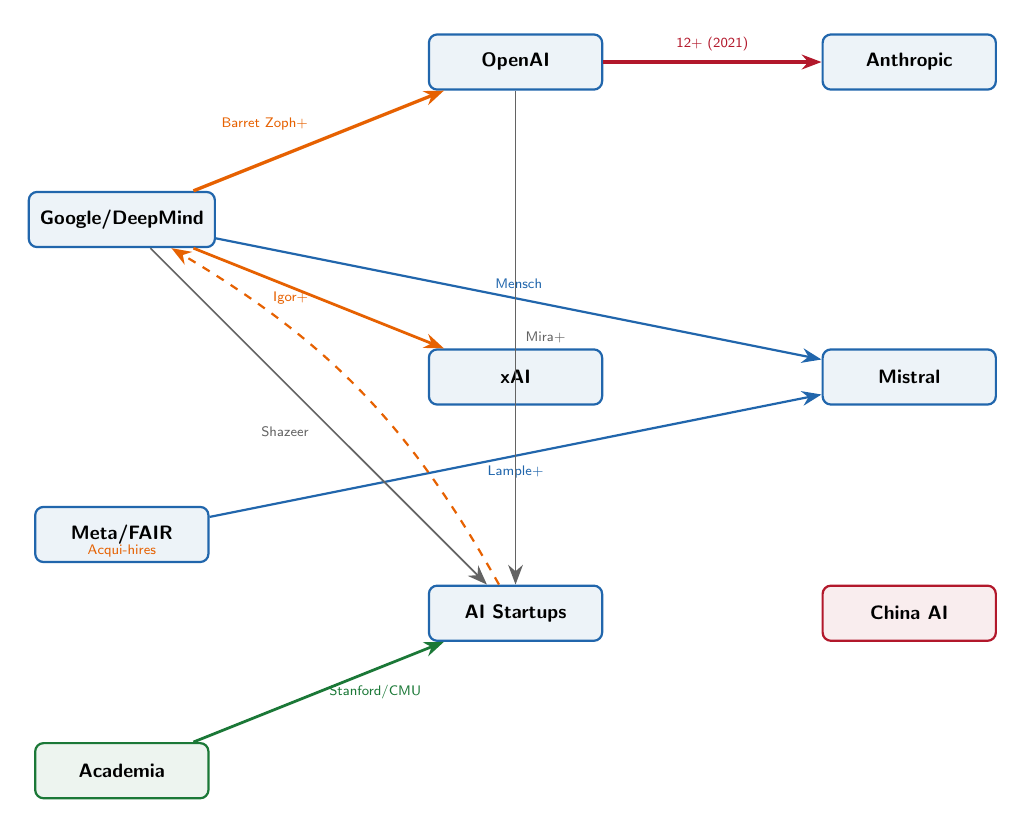
\begin{tikzpicture}[
  every node/.style={font=\sffamily\scriptsize},
  org/.style={draw=figBlue, thick, fill=figBlue!8, rounded corners=3pt,
              inner sep=4pt, font=\sffamily\scriptsize\bfseries,
              minimum width=2.2cm, minimum height=0.7cm},
  flow/.style={-{Stealth[length=2.5mm]}, thick},
]

% Organizations
\node[org] (google) at (0, 4) {Google/DeepMind};
\node[org] (openai) at (5, 6) {OpenAI};
\node[org] (anthropic) at (10, 6) {Anthropic};
\node[org] (meta) at (0, 0) {Meta/FAIR};
\node[org] (xai) at (5, 2) {xAI};
\node[org] (mistral) at (10, 2) {Mistral};
\node[org] (startups) at (5, -1) {AI Startups};
\node[org, draw=figRed, fill=figRed!8] (china) at (10, -1) {China AI};
\node[org, draw=figGreen, fill=figGreen!8] (academia) at (0, -3) {Academia};

% Flows (width indicates volume)
\draw[flow, figRed, line width=1.5pt] (openai) -- (anthropic)
  node[midway, above, font=\sffamily\tiny] {12+ (2021)};
\draw[flow, figOrange, line width=1.2pt] (google) -- (openai)
  node[midway, above left, font=\sffamily\tiny] {Barret Zoph+};
\draw[flow, figOrange, line width=1.0pt] (google) -- (xai)
  node[midway, left, font=\sffamily\tiny] {Igor+};
\draw[flow, figBlue, line width=0.8pt] (google) -- (mistral)
  node[midway, above, font=\sffamily\tiny] {Mensch};
\draw[flow, figBlue, line width=0.8pt] (meta) -- (mistral)
  node[midway, below, font=\sffamily\tiny] {Lample+};
\draw[flow, figGreen, line width=1.0pt] (academia) -- (startups)
  node[midway, right, font=\sffamily\tiny] {Stanford/CMU};
\draw[flow, figGray, line width=0.6pt] (openai) -- (startups)
  node[midway, right, font=\sffamily\tiny] {Mira+};
\draw[flow, figGray, line width=0.6pt] (google) -- (startups)
  node[midway, below left, font=\sffamily\tiny] {Shazeer};

% Return flows (dashed)
\draw[flow, dashed, figOrange, line width=0.8pt] (startups) to[bend right=15] (google)
  node[midway, below, font=\sffamily\tiny] {Acqui-hires};

\end{tikzpicture}
\caption{Major talent migration flows in the AI industry (2021--2026).
Arrow width roughly indicates the volume of migration.
The OpenAI $\to$ Anthropic flow (12+ researchers in 2021)
remains the single largest coordinated departure in AI history.}
\label{fig:talent-flows}
\end{figure}


\section{Reading Companion: Cross-References to Sister Publications}
\label{sec:appendix-xref}

\begin{table}[htbp]
\centering
\caption{Cross-reference guide to the LLM Observatory trilogy}
\label{tab:xref}
\begin{tabularx}{\textwidth}{lXX}
\hline
\textbf{This Book} & \textbf{Emergence} & \textbf{AI Startup Landscape} \\
\hline
\rowcolor{figLightGray}
Ch.\ 2 (Pioneers) & Ch.\ 2 (Transformer) & Ch.\ 1 (Overview) \\
Ch.\ 3 (OpenAI) & Ch.\ 8 (Post-Training) & Ch.\ 3 (Model Companies) \\
\rowcolor{figLightGray}
Ch.\ 4 (Anthropic) & Ch.\ 8 (Post-Training) & Ch.\ 3 (Model Companies) \\
Ch.\ 5 (Google) & Ch.\ 5--6 (Pretraining, MoE) & Ch.\ 3 (Model Companies) \\
\rowcolor{figLightGray}
Ch.\ 6 (Meta/OSS) & Ch.\ 5 (Pretraining) & Ch.\ 3 (Model Companies) \\
Ch.\ 8 (China) & Ch.\ 9 (Inference) & Ch.\ 11 (China Ecosystem) \\
\rowcolor{figLightGray}
Ch.\ 9 (Infra) & Ch.\ 9 (Inference) & Ch.\ 2 (Infrastructure) \\
Ch.\ 12 (Enterprise) & Ch.\ 15 (Agent Wars) & Ch.\ 10 (Enterprise) \\
\rowcolor{figLightGray}
Ch.\ 13 (Academics) & Ch.\ 12 (Team/Org) & --- \\
\hline
\end{tabularx}
\end{table}


\printbibliography[heading=bibintoc,title=References]

\end{document}
